\documentclass[titlepage,oneside,bookmarks,bookmarksnumbered,plainpages=false,pdfpagelabels]{book}
\usepackage{longtable}
\usepackage{html}

%begin{latexonly}
\usepackage{times}
\usepackage[latex2html,bookmarks,bookmarksnumbered,plainpages=false,pdfpagelabels]{hyperref}

%end{latexonly}

%
%  For use with latex2html
%
\usepackage{html}
\usepackage{graphicx}
\usepackage{makeidx}
\usepackage{upquote}
\usepackage[T1]{fontenc}
\usepackage{microtype}


%
%  Set the size of the margins and text area
%
\setlength{\evensidemargin}{0.25in}
\setlength{\oddsidemargin}{0.25in}
\setlength{\textwidth}{6.5in}
\setlength{\topmargin}{0.2in}
\setlength{\headsep}{0.5in}
\setlength{\topskip}{0in}
\setlength{\marginparwidth}{1in}
\setlength{\marginparsep}{0in}
\setlength{\footskip}{0.75in}
\newcommand{\ResetParaSpacing}{\setlength{\parskip}{.8em}}
\ResetParaSpacing

%
%  Let the figures take up more than half of the page
%

%begin{latexonly}
\renewcommand\floatpagefraction{.9}
\renewcommand\topfraction{.9}
\renewcommand\bottomfraction{.9}
\renewcommand\textfraction{.1}


%end{latexonly}

% Allow multiline labels.
\usepackage{enumitem}
\setlist{style=unboxed}

%
%  Bring in HTCondor macros
%
%
%  Set up version, author and copyright notices
%
\newcommand{\AuthorNotice}{Condor Team, University of Wisconsin--Madison}
\newcommand{\VersionNotice}{Version 6.6.4}
\newcommand{\CondorR}{Condor\textsuperscript{\scriptsize{\textregistered}}}
\newcommand{\CopyrightNotice}{Copyright \copyright\ 1990-2004 Condor Team, Computer Sciences Department, 
  University of Wisconsin-Madison, Madison, WI.  All Rights Reserved.  
  No use of the Condor Software Program is authorized 
  without the express consent of the Condor Team.  For more information 
  contact: Condor Team, Attention: Professor Miron Livny, 
  7367 Computer Sciences, 1210 W. Dayton St., Madison, WI 53706-1685, 
  (608) 262-0856 or miron@cs.wisc.edu.
 
  U.S. Government Rights Restrictions: Use, duplication, or disclosure 
  by the U.S. Government is subject to restrictions as set forth in 
  subparagraph (c)(1)(ii) of The Rights in Technical Data and Computer 
  Software clause at DFARS 252.227-7013 or subparagraphs (c)(1) and 
  (2) of Commercial Computer Software-Restricted Rights at 48 CFR 
  52.227-19, as applicable, Condor Team, Attention: Professor Miron 
  Livny, 7367 Computer Sciences, 1210 W. Dayton St., Madison, 
  WI 53706-1685, (608) 262-0856 or miron@cs.wisc.edu. 

  See the \emph{Condor \VersionNotice\ Manual} for
  additional notices. }

%
%  Common motifs
%
\newcommand{\Prog}[1]{\textit{#1}}              	% Program name
\newcommand{\Term}[1]{\emph{#1}}			% Use this to introduce terminology
\newcommand{\Cmd}[2]{\textit{#1}(#2)}           	% Command w/ section number
\newcommand{\Sinful}[1]{$<$#1$>$}         	% Sinful string
\newcommand{\SinfulAny}{$<$a.b.c.d:port$>$}        	% Arbitrary Sinful string
\newcommand{\URL}[1]{\htmladdnormallink{#1}{#1}}	% a URL
\newcommand{\Email}[1]{\htmladdnormallink{#1}{mailto:#1}}
\newcommand{\File}[1]{\texttt{#1}}        	    	% File name
\newcommand{\Bs}{$\mathtt{\backslash}$}         	% Backslash
% If we don't use math mode, latex2html can use the aux files generated for
% the PDF.  Doing so also eliminates a symlink.
\newcommand{\Bar}{{\tt |}}
\newcommand{\Dots}{\dots}
	% This brings in \Bar |, \Dots ...
\newcommand{\Tilde}{\~{}}                 	% tilde
\newcommand{\Circum}{\^{}}                      	% ^
\newcommand{\Lbr}{[}                            	% [
\newcommand{\Rbr}{]}                            	% ]
\newcommand{\Percent}{\%}                       	% %
\newcommand{\Opt}[1]{\mbox{\textbf{#1}}}            % Option
\newcommand{\Arg}[1]{\mbox{\textit{#1}}}            % Argument
\newcommand{\OptArg}[2]{\mbox{\Opt{#1\ }\Arg{#2}}}  % Option with Argument
\newcommand{\oArg}[1]{\mbox{[\Arg{#1}]}}            % optional Argument
\newcommand{\oOpt}[1]{\mbox{[\Opt{#1}]}}            % optional Option
\newcommand{\oOptArg}[2]{\mbox{[\OptArg{#1\ }{#2}]}}% optional Option w/ Arg
\newcommand{\Optnm}[1]{\textbf{#1}}            % Option w/o mbox
\newcommand{\Argnm}[1]{\textit{#1}}            % Argument w/o mbox
\newcommand{\OptArgnm}[2]{\Optnm{#1\ }\Argnm{#2}}% Option with Argument w/o mbox
\newcommand{\oArgnm}[1]{[\Argnm{#1}]}            % optional Argument w/o mbox
\newcommand{\oOptnm}[1]{[\Optnm{#1}]}            % optional Option w/o mbox
\newcommand{\oOptArgnm}[2]{[\OptArgnm{#1\ }{#2}]}% optional Option w/Arg w/o mbox
\newcommand{\Env}[1]{\texttt{#1}}		% Environment variable
\newcommand{\DCPerm}[1]{\texttt{#1}}		% DC Permission
\newcommand{\ShortExpr}[1]{\mbox{\texttt{#1}}}		% A pithy config file expression
\newcommand{\Expr}[1]{\texttt{#1}}		% Config file expression
\newcommand{\MacroNI}[1]{\texttt{#1}}		% Config file macro, NO index
\newcommand{\Macro}[1]{\texttt{#1} \index{#1 macro@\texttt{#1} macro} \index{configuration macro!\texttt{#1}}}		% Config file macro and index
\newcommand{\MacroUNI}[1]{\texttt{\$(#1)}}	% Config file macro's use, NO index
\newcommand{\MacroU}[1]{\texttt{\$(#1)}\index{#1 macro@\texttt{#1} macro}\index{configuration macro!\texttt{#1}}}	% Config file macro's use and index
\newcommand{\AdAttr}[1]{\texttt{#1}}	% ClassAd Attribute name
\newcommand{\Attr}[1]{\texttt{#1}}	% ClassAd Attribute name again
\newcommand{\AdStr}[1]{\texttt{"#1"}}	% ClassAd Attribute string
\newcommand{\Dflag}[1]{\texttt{D\_#1}}		% Debug flag name
\newcommand{\Bold}[1]{\textbf{#1}}		% Something you want bold
\input{fontsize.tex}
\newcommand{\Note}{\underline{NOTE}: }          % NOTE:
\newcommand{\Warn}{\underline{WARNING}: }       % WARNING:
\newcommand{\Todo}{\begin{center} \fbox{This section has not yet been written} \end{center}}
\newcommand{\Syscall}[1]{\texttt{#1()}}		% The name of a syscall

% A keyword in a meta-language
\newcommand{\Keyword}[1] {{\tt #1}}

% The name of a procedure
\newcommand{\Procedure}[1] {{\tt #1\(\)}}

% A program code snippet
\newcommand{\Code}[1] {{\tt #1}}

% Make a nice box with a header to point out a tricky feature
\newcommand{\Notice}[1] {\noindent {\bf Notice: }\\ \fbox{\parbox[t]{\textwidth}{#1}}}

% Release directory entry
\newcommand{\Release}[1]{\texttt{$<$release\_dir$>$/#1}}


%
% This sets the BODY tag when converted to HTML.
% It has no effect on the DVI file.
\bodytext{ BGCOLOR=#FFFFFF }

%
%  To help with typing in names of condor commands
%    e.g., condor_submit == \Condor{submit}
\newcommand{\Condor}[1]{\Prog{condor\_#1}}
\newcommand{\condor}[1]{condor\_#1}



\begin{htmlonly}
\input{fontsize.html.tex}
\end{htmlonly}

%begin{latexonly}
\input{fontsize.pdf.tex}
%end{latexonly}

%  Environment for a manual entry
%
\newenvironment{ManPage}[3]{% #1-Name, #2-Section, #3-Short description
  \newpage
  \latex
    {
	  \if@twoside
      \fancyhead[LE,RO]{\thepage} \fancyhead[RE,LO]{#1 (#2)}    % only on latex
	  \else
      \fancyhead[R]{\thepage} \fancyhead[L]{#1 (#2)}    % only on latex
      \fi
      \fancyfoot[C]{Condor \VersionNotice, Command Reference}
    }
  \section*{#1} #3
  % \latex{\addcontentsline{toc}{section}{#1\dotfill\ }}
  \latex{\addcontentsline{toc}{section}{#1}}
  \setlength{\parskip}{0.8em}
  \setlength{\parindent}{0em}
}{
  \subsection*{Author} \AuthorNotice
  \subsection*{Copyright} \CopyrightNotice
}

%
%  Parts of the man page
%
\newcommand{\Synopsis}{\subsection*{Synopsis}}          % Synopsis
\newcommand{\SynProg}[1]{\textbf{#1}}                   % Prog of the synopsis
\newcommand{\Description}{\subsection*{Description}}    % Description
\newenvironment{Options}{                               % Options table
  \subsection*{Options}
  \par
  \begin{description}
}{
  \end{description}
  \par
}

\newcommand{\OptItem}[2]{\item[#1] #2\\}                % Item in option table
\newcommand{\Examples}{\subsection*{Examples}}          % Examples
\newcommand{\Files}{\subsection*{Files}}                % Related files
\newcommand{\SeeAlso}{\subsection*{See Also}}           % See Also
\newcommand{\GenRem}{\subsection*{General Remarks}}     % General remarks
\newcommand{\ExitStatus}{\subsection*{Exit Status}} 	% Exit Status



% hyphenation of our terms
\hyphenation{Class-Ads Class-Ad}

%
%  Fix the headers and footers
%
\latex{
	\usepackage{fancyhdr}
	\pagestyle{fancy}
	\fancyhf{}
	\renewcommand{\sectionmark}[1]{\markright{\thesection.\ #1}}
	\renewcommand{\subsectionmark}[1]{\markright{\thesubsection.\ #1}}
\if@twoside
	\fancyhead[LE,RO]{\thepage}
	\fancyhead[RE]{\leftmark}
	\fancyhead[LO]{\rightmark}
\else
	\fancyhead[R]{\thepage}
	\fancyhead[L]{\rightmark}
\fi

	\fancyfoot[C]{HTCondor \VersionNotice\ Manual}
	\renewcommand{\headrulewidth}{0.4pt}
	\renewcommand{\footrulewidth}{0.4pt}
	\addtolength{\headwidth}{\oddsidemargin}

}


% generate index
\makeindex

% This turns off the hbox underfull warnings, but
% does not change the formatting of the text
% default value is 1000
\hbadness=10000

\begin{document}

% Only to suppress a pdflatex warning.
\pagenumbering{Alph}

\title{HTCondor\textsuperscript{\small{\texttrademark}} \VersionNotice\ Manual}
\author{\AuthorNotice}
\maketitle

\pagenumbering{roman}

\tableofcontents

\sloppy

\begin{small}
%%%%%%%%%%%%%%%%%%%%%%%%%%%%%%%%%%%%%%%%%%%%%%%%%%%%%%%%%%%%%%%%%%%%%%%%%%%
\subsubsection{\label{sec:license}LICENSING AND COPYRIGHT}
%%%%%%%%%%%%%%%%%%%%%%%%%%%%%%%%%%%%%%%%%%%%%%%%%%%%%%%%%%%%%%%%%%%%%%%%%%%

HTCondor is released under the Apache License, Version 2.0.

\begin{flushleft}
Apache License \\
Version 2.0, January 2004\\
\URL{http://www.apache.org/licenses/}
\end{flushleft}

Copyright \copyright\ 1990-2018 Center for High Throughput Computing, 
Computer Sciences Department,
University of Wisconsin-Madison, WI. 

Licensed under the Apache License, Version 2.0 (the "License");
you may not use this file except in compliance with the License.
You may obtain a copy of the License at

\URL{http://www.apache.org/licenses/LICENSE-2.0}

Unless required by applicable law or agreed to in writing, software
distributed under the License is distributed on an "AS IS" BASIS,
WITHOUT WARRANTIES OR CONDITIONS OF ANY KIND, either express or implied.
See the License for the specific language governing permissions and
limitations under the License.

For complete information and additional license notices see

\URL{http://htcondor.org/license.html}


\end{small}

\newpage
\pagenumbering{arabic}

\chapter{Overview}
\label{overview}

This chapter provides a basic, high-level overview of Condor, including
Condor's major features and limitations. Because Condor is a system to
implement a High-Throughput Computing environment, this section begins
defining what is meant by High-Throughput Computing.


\section{What is High-Throughput Computing (HTC) ?}

\index{Condor!overview|(}
\index{overview|(}
For many research and engineering projects, the quality of the research
or the product is heavily dependent upon the quantity of computing
cycles available. It is not uncommon to find problems that require weeks
or months of computation to solve. Scientists and engineers engaged in
this sort of work need a computing environment that delivers large
amounts of computational power over a long period of time. Such an
environment is called a High-Throughput Computing (HTC) environment.
\index{High-Throughput Computing (HTC)}
\index{HTC (High-Throughput Computing)}
In contrast, High Performance Computing (HPC)
\index{High-Performance Computing (HPC)}
\index{HPC (High-Performance Computing)}
environments deliver a
tremendous amount of compute power over a short period of time. HPC
environments are often measured in terms of FLoating point Operations
per Second (FLOPS). 
A growing community is not concerned about FLOPS,
as their problems are of a much larger scale.
These people are
concerned with floating point operations per month or per year.
They are
more interested in how many jobs they can complete over a long period of
time instead of how fast an individual job can complete.

\section{HTC and Distributed Ownership}

The key to HTC is to efficiently harness the use of all available
resources. Years ago, the engineering and scientific community relied on
large centralized mainframe and/or big-iron supercomputers to do
computational work. A large number of individuals and groups needed
to pool their financial resources to afford such a machine. Users had
to wait for their turn on the mainframe, 
and they only had a certain amount of time allocated to them.
While this environment was
inconvenient for users, it was very efficient, because the mainframe
was busy nearly all the time.

As computers became smaller, faster, and cheaper, users moved
away from centralized mainframes and purchased personal desktop
workstations and PCs. An individual or small group could afford a
computing resource that was available whenever they wanted it. The
personal computer was
usually far slower than the large centralized machine, but it
was worthwhile due to its
exclusive access.
Now, instead of one giant
computer for a large institution, there might be hundreds or thousands
of personal computers. This is an environment of distributed ownership,
\index{distributed ownership!of machines}
where individuals throughout an organization own their own resources.
The total computational power of the institution as a whole might rise
dramatically as the result of such a change, but because of distributed
ownership, individuals could not capitalize on the institutional growth of
computing power. And while distributed ownership is more convenient for
the users, it is much less efficient. Many personal desktop
machines sit idle for very long periods of time while their owners are
busy doing other things (such as being away at lunch, in meetings,
or at home sleeping). 

\section{\label{sec:what-is-condor}What is Condor ?}

Condor is a software system that creates a High-Throughput Computing
(HTC) environment by effectively harnessing the power of a cluster of
UNIX or NT workstations on a network. Although Condor can manage a
dedicated cluster of workstations, a key appeal of Condor is its
ability to effectively harness non-dedicated, preexisting resources in
a distributed ownership 
\index{distributed ownership!of machines}
setting such as machines sitting on people's desks
in offices and labs. 

\subsection{A Hunter of Available Workstations}

Instead of running a CPU-intensive job in the background on their own
workstation, a user submits their job to Condor. Condor finds an
available machine on the network and begins running the job on
that machine. When Condor detects that a machine running a Condor job
is no longer available (perhaps because the owner of the machine
came back from lunch and started typing on the keyboard), Condor
checkpoints 
\index{checkpoint}
the job and migrates 
\index{migration}
it over the network to a
different machine which would otherwise be idle. Condor restarts
the job on the new machine to continue from precisely where it left off.
If no
machine on the network is currently available, then the job is stored in
a queue on disk until a machine becomes available.

As an example, a compute job that typically takes 5
hours to run is submitted to Condor.
Condor may start running the job on Machine A, but after 3
hours Condor detects activity on the keyboard.
Condor will checkpoint
the job and migrates it to Machine B.
After two hours on Machine B,
the job completes (notifying the submitter via e-mail). 

Perhaps this 5 hour compute job must be run 250 different times
\index{job!multiple data sets}
(perhaps on 250 different data sets).
In this case, Condor can be a real time saver.
With one command, all 250 runs are submitted to Condor.
Depending upon the number of machines in the organization's Condor
pool, there could be dozens or even hundreds of otherwise idle machines
running the job at any given moment.

Condor makes it easy to maximize the number of machines which can run
a job. Because Condor does not require participating machines to
share file systems (via NFS or AFS for example), machines across the
entire enterprise can run a job, including machines in different
administrative domains.
Condor does not require an
account (login) on machines where it runs a job.
Condor can do this
because of its \Term{remote system call}
\index{remote system call}
technology, which traps
operating system calls for such operations as reading or writing from disk
files and sends them back over the network to be performed on the machine
where the job was submitted. 

\subsection{Effective Resource Management}

In addition to migrating jobs to available machines, Condor provides
sophisticated and distributed resource management.
\index{Condor!resource management}
\index{resource!management}
Match-making resource
\index{matchmaking}
owners with resource consumers is the cornerstone of a successful HTC
environment.
Unlike many other compute cluster resource management
systems which attach properties to the job queues themselves (resulting
in user confusion over which queue to use as well as administrative
hassle in constantly adding and editing queue properties to satisfy user
demands), Condor implements a clean design called \Term{ClassAds}. 
\index{ClassAd}

ClassAds work in a fashion similar to the newspaper classified
advertising want-ads. All machines in the Condor pool advertise their
resource properties, such as available RAM memory, CPU type and speed,
virtual memory size, physical location, current load average, and many
other static and dynamic properties, into a \Term{resource offer} ad.
\index{resource!offer}
Likewise,
when submitting a job, users can specify a \Term{resource request} ad
\index{resource!request}
which
defines both the required and a desired set of properties to run the job.
Similarly, a resource offer ad can define requirements and preferences.
Condor acts as a broker by matching and ranking resource
offer ads with resource request ads, making certain that all
requirements in both ads are satisfied. During this match-making
process, Condor also takes several layers of priority values into
consideration: the priority the user assigned to the resource request
ad, the priority of the user which submitted the ad, and desire of
machines in the pool to accept certain types of ads over others. 

\section{Distinguishing Features}

\begin{description}
	\item[Checkpoint and Migration.] Users of Condor may be assured that
their jobs will eventually complete even in an opportunistic computing
environment. If a user submits a job to Condor which runs on another's
workstation, but the job is not finished when the workstation
owner returns, the job can be checkpointed.
\index{checkpoint}
The job continues
by migrating 
\index{migration}
to another machine. It makes progress toward
its completion by the checkpoint and migration feature.
Condor's periodic checkpoint feature 
\index{checkpoint!periodic}
periodically checkpoints a job even in lieu of migration in order to
safeguard the accumulated computation time on a job from being lost in the
event of a system failure such as the machine being shutdown or a crash.
	\item[Remote System Calls.] 
\index{remote system call}
Despite running jobs on remote machines,
the Condor standard universe execution
mode preserves the local execution environment
via remote system calls. Users do not have to worry
about making data files available to remote workstations or even
obtaining a login account on remote workstations before Condor executes
their programs there. The program behaves under Condor as if it were
running as the user that submitted the job on the workstation where it
was originally submitted, no matter on which machine it really ends up
executing on.
	\item[No Changes Necessary to User's Source Code.] No special
programming is required to use Condor. Condor is able to run normal
non-interactive UNIX or NT programs.  The checkpoint and migration of
programs by Condor is transparent and automatic, as is the use of
remote system calls.  If these facilities are desired, the user only
re-links the program.  The code is not compiled or changed.
	\item[Sensitive to the Desires of Workstation Owners.] The
owner of a
workstation has complete priority over the workstation,
by default.
A workstation owner is generally happy to let others compute on
the workstation while it is idle, but wants the workstation back
promptly upon returning. The owner does not want to take special
action to regain control. Condor handles this automatically. 
	\item[ClassAds.]The ClassAd mechanism 
\index{ClassAd}
in Condor provides an extremely
flexible, expressive framework for matchmaking
resource requests with resource offers. One result is that users can
easily request practically any resource, both in terms of job
requirements and job desires.
For example, a user can require that a job run on a machine
with 64 Mbytes of RAM,
but state a preference for 128 Mbytes if available.
Likewise, a workstation
can state a preference in a resource offer to run jobs
from a specified set of users, and it can require that there be
no interactive workstation
activity detectable between 9 am and 5 pm before starting a job.
Job requirements/preferences and resource availability constraints can be
described in terms of powerful expressions, resulting in
Condor's adaptation to nearly any desired policy. 
\end{description}
\index{Condor!overview|)}
\index{overview|)}

\section{\label{sec:current-limitations}Current Limitations}

\begin{description}

\index{Condor!limitations, under UNIX}
	\item[Limitations on Jobs which can Checkpointed] Although Condor can schedule and
run any type of process, Condor does have some limitations on jobs that it can
transparently checkpoint and migrate:


\begin{enumerate}

\index{Unix!fork}
\index{Unix!exec}
\index{Unix!system}
\item Multi-process jobs are not allowed.  This includes system calls such as
\Syscall{fork}, \Syscall{exec}, and \Syscall{system}.

\index{Unix!pipe}
\index{Unix!semaphore}
\index{Unix!shared memory}
\item Interprocess communication is not allowed.  This includes pipes, semaphores, and shared memory.

\index{Unix!socket}
\index{network}
\item Network communication must be brief.  A job \emph{may} make network
connections using system calls such as \Syscall{socket}, but a network
connection left open for long periods will delay checkpointing and migration.

\index{signal}
\index{signal!SIGUSR2}
\index{signal!SIGTSTP}
\item Sending or receiving the SIGUSR2 or SIGTSTP signals is not allowed.
HTCondor reserves these signals for its own use.  Sending or receiving all
other signals \emph{is} allowed.

\index{Unix!alarm}
\index{Unix!timer}
\index{Unix!sleep}
\item Alarms, timers, and sleeping are not allowed.  This includes system
calls such as \Syscall{alarm}, \Syscall{getitimer}, and \Syscall{sleep}.

\index{thread!kernel-level}
\index{thread!user-level}
\item Multiple kernel-level threads are not allowed.  However,
multiple user-level threads \emph{are} allowed.

\index{file!memory-mapped}
\index{Unix!mmap}
\item Memory mapped files are not allowed.  This includes system calls such
as \Syscall{mmap} and \Syscall{munmap}.

\index{file!locking}
\index{Unix!flock}
\index{Unix!lockf}
\item File locks are allowed, but not retained between checkpoints.

\index{file!read only}
\index{file!write only}
\item All files must be opened read-only or write-only.  A file opened
for both reading and writing will cause trouble if a job must be rolled back
to an old checkpoint image.  For compatibility reasons, a file opened
for both reading and writing will result in a warning but not an error.

\item A fair amount of disk space must be available on the submitting machine
for storing a job's checkpoint images.  A checkpoint image is approximately
equal to the virtual memory consumed by a job while it runs.  If disk space
is short, a special \Term{checkpoint server} can be designated for storing
all the checkpoint images for a pool.

\index{linking!dynamic}
\index{linking!static}
\item On Linux, the job must be statically linked. 
\Condor{compile} does this by default.

\index{Unix!large files} 
\item Reading to or writing from files larger than 2 GBytes is only supported
when the submit side \Condor{shadow} and the standard universe user job
application itself are both 64-bit executables.

\end{enumerate}





	Note: these limitations \emph{only} apply to jobs which Condor
has been asked to transparently checkpoint.  If job checkpointing is not
desired, the limitations above do not apply.

	\item[Security Implications.] Condor does a significant amount of work to prevent 
security hazards, but loopholes are known to exist.  Condor can be instructed 
to run user programs only as the UNIX user nobody, a user login which traditionally has very 
restricted access.  But even with access solely as user nobody, a sufficiently 
malicious individual could do such things as fill up /tmp (which is world writable) and/or gain 
read access to world readable files.
Furthermore, where the security of machines in the pool is a high concern, 
only machines where the UNIX user root on that machine can be trusted should be admitted
into the pool. Condor provides the administrator with IP-based security mechanisms 
to enforce this.

	\item[Jobs Need to be Re-linked to get Checkpointing and Remote System Calls] Although 
typically no source code changes are required,
Condor requires
that the jobs be re-linked with the Condor libraries to take
advantage of checkpointing and remote system calls. This often
precludes commercial software binaries from taking advantage of these services
because commercial packages rarely make their object code
available. 
Condor's other services are still available for these commercial packages.

\end{description}

\section{\label{sec:Availability}Availability}
\index{Condor!availability}
Condor is currently available as a free download from the Internet via the World Wide Web at  
URL \Url{http://www.cs.wisc.edu/condor/downloads}.
Binary distributions of Condor version 6.x are available for the platforms 
detailed in Table~\ref{supported-platforms}.  A platform is an 
architecture/operating system combination.  
Condor binaries are available most major versions of UNIX, as well as
Windows NT.  

In the table, \Term{clipped} means that Condor does not support
checkpointing or remote system calls on the given platform. 
This means that \Term{standard} jobs are not supported, only
\Term{vanilla} jobs.
See section~\ref{sec:Choosing-Universe} on
page~\pageref{sec:Choosing-Universe} for more details on job universes
within Condor and their abilities and limitations.

The Condor source code is no longer available for public download from the Internet.  If you 
desire the Condor source code, please contact the Condor Team in order to discuss it further 
(see Section~\ref{contact-info}, on page~\pageref{contact-info}).

\begin{center}
\begin{table}[hbt]
\begin{tabular}{|ll|} \hline
\emph{Architecture} & \emph{Operating System} \\ \hline \hline
Hewlett Packard PA-RISC (both PA7000 and PA8000 series) & HPUX 10.20 \\ \hline
Sun SPARC Sun4{m,c}, Sun UltraSPARC & Solaris 2.5.x, 2.6, 2.7 \\ \hline
Silicon Graphics MIPS (R4400, R4600, R8000, R10000) & IRIX 6.2, 6.3, 6.4 \\ 
 & IRIX 6.5 \\ \hline
Intel x86 & Linux 2.0.x, 2.2.x, glibc20, glibc21, libc5 \\
 & Solaris 2.5.x, 2.6, 2.7 \\ 
 & Windows NT 4.0 (``clipped'') \\ \hline
Digital ALPHA & OSF/1 (Digital Unix) 4.x \\
 & Linux 2.0.x, Linux 2.2.x (``clipped'') \\ \hline
\end{tabular}
\caption{\label{supported-platforms}Condor \VersionNotice\ supported platforms}
\end{table}
\end{center}

%%%%%%%%%%%%%%%%%%%%%%%%%%%%%%%%%%%%%%%%%%%%%%%%%%%%%%%%%%%%%%%%%%%%%%
\section{\label{sec:Version-History}Version History}
%%%%%%%%%%%%%%%%%%%%%%%%%%%%%%%%%%%%%%%%%%%%%%%%%%%%%%%%%%%%%%%%%%%%%%

This section provides descriptions of what features have been added or
bugs fixed for each version of Condor.  
Each release series is covered in its own section.

%%%%%%%%%%%%%%%%%%%%%%%%%%%%%%%%%%%%%%%%%%%%%%%%%%%%%%%%%%%%%%%%%%%%%%
\subsection{\label{sec:History-6-1}Development Release Series 6.1}
%%%%%%%%%%%%%%%%%%%%%%%%%%%%%%%%%%%%%%%%%%%%%%%%%%%%%%%%%%%%%%%%%%%%%%

This is the first development release.
You should only install it if you really know what you are doing.
Development releases will come out quickly, with lots of new features
being added, many bugs fixed, etc.  
6.1.X should not be used for a production pool.

\Note Different releases within a development series cannot be
installed side-by-side within the same pool. 
For example, the protocols used by version 6.1.6 are not compatible with the
protocols used in version 6.1.5.  
When you upgrade to a new development release, make certain you upgrade all
machines in your pool to the same version.

%%%%%%%%%%%%%%%%%%%%%%%%%%%%%%%%%%%%%%%%%%%%%%%%%%%%%%%%%%%%%%%%%%%%%%
\subsubsection{\label{sec:New-6-1-11}Version 6.1.11}
%%%%%%%%%%%%%%%%%%%%%%%%%%%%%%%%%%%%%%%%%%%%%%%%%%%%%%%%%%%%%%%%%%%%%%

\noindent New Features:

\begin{itemize}

\item \Condor{q} has been fixed to be faster and much more memory
efficient.  This is much more obvous when getting the queue from
\Condor{schedd}'s that have more than 1000 jobs.

\item Added support for support for socket() and pipe() in standard
jobs.  Both sockets and pipes are created on the executing machine.
Checkpointing is deferred anytime a socket or pipe is open.

\item Added limited support for select() and poll() in standard jobs.
Both calls will work on files opened locally.

\item Added limited support for fcntl() and ioctl() in standard jobs.
Both calls will be performed remotely if the control-number is understood
and the third argument is an integer.

\item Replaced buffer implementation in standard jobs.
The new buffer code reads and writes variable sized chunks.
It will never issue a read to satisfy a write.  Buffering is enabled
by default.

\item Added extensive feedback on I/O performance in the user's email.

\item Added -io option to \Condor{q} to show I/O statistics.

\end{itemize}

\noindent Bugs Fixed:

\begin{itemize}

\item None.

\end{itemize}

\noindent Known Bugs:

\begin{itemize}

\item None.

\end{itemize}

%%%%%%%%%%%%%%%%%%%%%%%%%%%%%%%%%%%%%%%%%%%%%%%%%%%%%%%%%%%%%%%%%%%%%%
\subsubsection{\label{sec:New-6-1-10}Version 6.1.10}
%%%%%%%%%%%%%%%%%%%%%%%%%%%%%%%%%%%%%%%%%%%%%%%%%%%%%%%%%%%%%%%%%%%%%%

\noindent New Features:

\begin{itemize}

\item \Condor{q} now accepts \texttt{-format} parameters like \Condor{status}

\item \Condor{rm}, \Condor{hold} and \Condor{release} accept
  \texttt{-constraint} parameters like \Condor{status}

\item \Condor{status} now sorts displayed totals by the first column.
(This feature introduced a bug in \Condor{status}.  See ``Known Bugs''
below.)

\item Condor version 6.1.10 introduces ``clipped'' support for Sparc
Solaris version 2.7.
This version does not support checkpointing or remote system calls.
Full support for Solaris 2.7 will be released soon.

\item Introduced code to enable Linux to use the standard C library's
I/O buffering again, instead of relying on the Condor I/O buffering
code (which is still in beta testing).  

\end{itemize}

\noindent Bugs Fixed:

\begin{itemize}

\item The bug in checkpointing introduced in version 6.1.9 has been
fixed.
Checkpointing will now work on all platforms, as it always used to.  
Any jobs linked with the 6.1.9 Condor libraries will need to be
relinked with \Condor{compile} once version 6.1.10 has been installed
at your site. 

\end{itemize}

\noindent Known Bugs:

\begin{itemize}

\item The \AdAttr{CondorLoadAvg} attribute in the \Condor{startd} has
some problems in the way it is computed.
The CondorLoadAvg is somewhat inaccurate for the first minute a job
starts running, and for the first minute after it completes.
Also, the computation of CondorLoadAvg is very wrong on NT.
All of this will be fixed in a future version.

\item A memory error may cause \Condor{status} to die with SIGSEGV
(segmentation violation) when displaying totals or cause incorrect
totals to be displayed.  This will be fixed in version 6.1.11.

\end{itemize}


%%%%%%%%%%%%%%%%%%%%%%%%%%%%%%%%%%%%%%%%%%%%%%%%%%%%%%%%%%%%%%%%%%%%%%
\subsubsection{\label{sec:New-6-1-9}Version 6.1.9}
%%%%%%%%%%%%%%%%%%%%%%%%%%%%%%%%%%%%%%%%%%%%%%%%%%%%%%%%%%%%%%%%%%%%%%

\noindent New Features:

\begin{itemize}

\item Added full support for Linux 2.0.x and 2.2.x kernels using
libc5, glibc20 and glibc21.
This includes support for RedHat 6.x, Debian 2.x and other popular
Linux distributions.
Whereas the Linux machines had once been fragmented across libc5 and
GNU libc, they have now been reunified.
This means there is no longer any need for the ``LINUX-GLIBC'' OpSys
setting in your pool: all machines will now show up as ``LINUX''.
Part of this reunification process was the removal of dynamically
linked user jobs on Linux.
\Condor{compile} now forces static linking of your Standard Universe
Condor jobs. 
Also, please use \Condor{compile} on the same machine on which you
compiled your object files.

\item Added \Condor{qedit} utility to allow users to modify job
attributes after submission.  See the new manual page on
page~\pageref{man-condor-qedit}.

\item Added \OptArg{{-runfor}{minutes}} option to daemonCore to have
the daemon gracefully shut down after the given number of minutes.

\item Added support for statfs(2) and fstatfs(2) in user jobs. We support 
only the fields
\textit{f\_bsize, f\_blocks, f\_bfree, f\_bavail, f\_files, f\_ffree} from
the structure statfs. This is still in the experimental stage.

\item Added the \Opt{-direct} option to \Condor{status}.
After you give \Opt{-direct}, you supply a hostname, and
\Condor{status} will query the \Condor{startd} on the specified host
and display information directly from there, instead of querying the
\Condor{collector}.
See the manual page on page~\pageref{man-condor-submit} for details. 

\item Users can now define \Macro{NUM\_CPUS} to override the automatic
computation of the number of CPUs in your machine.
Using this config setting can cause unexpected results, and is not
recommended. 
This feature is only provided for sites that specifically want this
behavior and know what they are doing.

\item The \Opt{-set} and \Opt{-rset} options to \Condor{config\_val}
have been changed to allow administrators to set both macros and
expressions.
Previously, \Condor{config\_val} assumed you wanted to set
expressions.
Now, these two options each take a single argument, the string
containing exactly what you would put into the config file, so you can
specify you want to create a macro by including an ``='' sign, or an
expression by including a ``:''.
See section~\ref{sec:Intro-to-Config-Files} on
page~\pageref{sec:Intro-to-Config-Files} for details on macros
vs. expressions.
See the \Condor{config\_val} man page on
page~\pageref{man:condor-config-val} for details on
\Condor{config\_val}.  

\item If the directory you specified for LOCK (which holds lock files
used by Condor) doesn't exist, Condor will now try to create that
directory for you instead of giving up right away.

\item If you change the \Attr{COLLECTOR\_HOST} setting and reconfig
the \Condor{startd}, the startd will ``invalidate'' its ClassAds at
the old collector before it starts reporting to the new one.

\end{itemize}

\noindent Bugs Fixed:

\begin{itemize}

\item Fixed a major bug dealing with the group access a Condor job is
started with.
Now, Condor jobs are started with all the groups the job's owner is
in, not just their default group.
This also fixes a security hole where user jobs could be started up in
access groups they didn't belong to.

\item Fixed a bug where there was a needless limitation on the number of open
file descriptors a user job could have.

\item Fixed a standalone checkpointing bug where we weren't blocking signals
in critical sections and causing file table corruption at checkpoint
time.

\item Fixed a linker bug on Digital Unix 4.0 concerning fortran where
the linker would fail on \_\_uname and \_\_sigsuspend.

\item Fixed a bug in \Condor{shadow} that would send incorrect job
completion email under Linux.

\item Fixed a bug in the remote system call of \Syscall{fchdir} that caused
a garbage file descriptor to be used in Standard Universe jobs.

\item Fixed a bug in the \Condor{shadow} which was causing \Condor{q}
\Opt{-goodput} to display incorrect values for some jobs.

\item Fixed some minor bugs and made some minor enhancements in the
\Condor{install} script.
The bugs included a typo in one of the questions asked, and incorrect
handling for the answers of a few different questions.
Also, if DNS is misconfigured on your system, \Condor{install} will
try a few ways to find your fully qualified hostname, and if it still
can't determine the correct hostname, it will prompt the user for it. 
In addition, we now avoid one installation step in cases were it is
not needed. 

\item Fixed a rare race condition that could delay the completion of
large clusters of short running jobs. 

\item Added more checking to the various arguments that might be
passed to \Condor{status}, so that in the case of bad input,
\Condor{status} will print an error message and exit, instead of
performing a segmentation fault.
Also, when you use the \Opt{-sort} option, \Condor{status} will only
display ClassAds where the attributes you use to sort are defined.

\item Fixed a bug in the handling of the config files created by
using the \Opt{-set} or \Opt{-rset} options to \Condor{config\_val}.
Previously, if you manually deleted the files that were created, you
could cause the affected Condor daemon to have a segmentation fault.
Now, the daemons simply exit with a fatal error but still have a
chance to clean up.

\item Fixed a bug in the \Opt{-negotiator} option for most Condor
tools that was causing it to get the wrong address.

\item Fixed a couple of bugs in the \Condor{master} that could cause
improper shutdowns. 
There were cases during shutdown where we would restart a daemon
(because we previously noticed a new executable, for example).
Now, once you begin a shutdown, the \Condor{master} will not restart
anything. 
Also, fixed a rare bug that could cause the \Condor{master} to stop
checking the timestamps on a daemon.

\item Fixed a minor bug in the \Opt{-owner} option to
\Condor{config\_val} that was causing \Condor{init} not to work.

\item Fixed a bug where the \Condor{startd}, while it was already
shutting down, was allowing certain actions to succeed that should
have failed.
For example, it allowed itself to be matched with a user looking for
available machines, or to begin a new PVM task.

\end{itemize}

\noindent Known Bugs:

\begin{itemize}

\item The \AdAttr{CondorLoadAvg} attribute in the \Condor{startd} has
some problems in the way it is computed.
The CondorLoadAvg is somewhat inaccurate for the first minute a job
starts running, and for the first minute after it completes.
Also, the computation of CondorLoadAvg is very wrong on NT.
All of this will be fixed in a future version.

\item There is a serious bug in checkpointing when using Condor's
I/O buffering for ``standard'' jobs.
By default, Linux uses Condor buffering in version 6.1.9 for all
standard jobs.
The bug prevents checkpointing from working more than once.
This renders the \Condor{vacate} and \Condor{checkpoint} commands
useless, and jobs will just be killed without a checkpoint when
machine owners come back to their machines.

\end{itemize}


%%%%%%%%%%%%%%%%%%%%%%%%%%%%%%%%%%%%%%%%%%%%%%%%%%%%%%%%%%%%%%%%%%%%%%
\subsubsection{\label{sec:New-6-1-8}Version 6.1.8}
%%%%%%%%%%%%%%%%%%%%%%%%%%%%%%%%%%%%%%%%%%%%%%%%%%%%%%%%%%%%%%%%%%%%%%

\begin{itemize}

\item Added \Term{file\_remaps} as command in the job submit file given to
STANDARD universe jobs.
A Job can now specify that it would like to have files be remapped
from one file to another.
In addition you can specify that files should be read from the local machine
by specifing them.
See the \Condor{submit} manual page on page~\pageref{man-condor-submit} for
more details.

\item Added \Term{buffer\_size} and \Term{buffer\_block\_size} so that STANDARD
universe jobs can specify that they wish to have I/O buffering turned on.
Without buffering, all I/O requests in the STANDARD universe are sent back
over the network to be executed on the submit machine.  
With buffering, read ahead, write behind, and seek batch buffering is
performed to minimize network traffic and latency.
By default, jobs do not specify buffering, however, for many situations buffering
can drastically increase throughput.  See the \Condor{submit} manual page
on page~\pageref{man-condor-submit} for more details.

\item The \Condor{schedd} is much more memory efficient handling clusters
with hundreds/thousands of jobs.  
If you submit large clusters, your submit machine will only use a fraction
of the amount of RAM it used to require.  
\Note The memory savings will only be realized for new clusters submitted
after the upgrade to v6.1.8 -- clusters which previously existed in the
queue at upgrade time will still use the same amount of RAM in the
\Condor{schedd}.

\item Submitting jobs, especially submitting large clusters containing many
jobs, is much faster.

\item Added a \Opt{-goodput} option to \Condor{q}, which displays
statistics about the execution efficiency of STANDARD universe jobs.

\item Added FS\_REMOTE method of user authentication to possible values
of the configuration option \Macro{AUTHENTICATION\_METHODS} to fix problems
with using the \Opt{-r} remote scheduler option of \Condor{submit}.
Additionally, the user authentication protocol has changed, so previous
versions of Condor programs cannot co-exist with this new protocol.

\item Added a new utility and documentation for \Condor{glidein} which uses 
Globus resources to extend your local pool to use remote Globus machines as 
part of your Condor pool.

\item Fixed more bugs in the handling of the stat() system call
and its relatives on Linux with glibc.
This was causing problems mainly with Fortran I/O, though other I/O
related problems on glibc Linux will probably be solved now.

\item Fixed a bug in various Condor tools (\Condor{status},
\Condor{user\_prio}, \Condor{config\_val}, and \Condor{stats}) that
would cause them to seg fault on bad input to the \Opt{-pool} option. 

\item Fixed a bug with the \Opt{-rset} option to \Condor{config\_val} which
could crash the Condor daemon whose configuration was being changed.

\item Added \Term{allow\_startup\_script} command to the job submit
description file which is given to \Condor{submit}.  This allows the
submission of a startup script to the STANDARD universe.  See 

\item Fixed a bug in the \Condor{schedd} where it would get into an
infinite loop if the persistant log of the job queue got corrupted.  
The \Condor{schedd} now correctly handles corrupted log files.

\item The full release tar file now contains a \File{dagman}
subdirectory in the \File{examples} directory.
This subdirectory includes an example DAGMan job, including a README
(in both ASCII and HTML), a Makefile, and so on.

\item Condor will now insert an environment variable, \Env{CONDOR\_VM}, into
the environment of the user job.  
This variable specifies which SMP ``virtual machine'' the job was started on.
It will equal either vm1, vm2, vm3, \Dots , depending upon which virtual
machine was matched.
On a non-SMP machine, \Env{CONDOR\_VM} will always be set to vm1.

\item Fixed some timing bugs introduced in v6.1.6 which could occur when
Condor tries to simultaneously start a large number of jobs submitted from a
single machine.

\item Fixed bugs when Condor is told to gracefully shutdown; Condor no
longer starts up new jobs when shutting down.  Also, the \Condor{schedd}
progressively checkpoints running jobs during a graceful shutdown instead of
trying to vacate all the job simultaneously.  The rate at which the shutdown
occurs is controlled by the \Macro{JOB\_START\_DELAY} configuration
parameter (see page~\pageref{param:JobStartDelay}).

\item Fixed a bug which could cause the \Condor{master} process to exit if
the Condor daemons have been hung for a while by the operating system (if,
for instance, the LOG directory was placed on an NFS volume and the NFS
server is down for an extended period).

\item Previously, removing a large number of jobs with \Condor{rm} would
result in the \Condor{schedd} being unresponsive for a period of time
(perhaps leading to timeouts when running \Condor{q}).  The \Condor{schedd}
has been improved to multitask the removal of jobs while servicing new
requests.

\item Added new configuration parameter \Macro{COLLECTOR\_SOCKET\_BUFSIZE}
which controls the size of TCP/IP buffers used by the \Condor{collector}.
For more info, see section~ref{param:CollectorSocketBufsize} on
page~pageref{param:CollectorSocketBufsize}.

\item Fixed a bug with the \Opt{-analyze} option to \Condor{q}: in some
cases, the RANK expression would not be evaluated correctly.  This could
cause the output from \Opt{-analyze} to be in error.

\item When running on a multi-CPU (SMP) Hewlett-Packard machine, fixed bugs
computing the system load average.

\item Fixed bug in \Condor{q} which could cause the RUN\_TIME reported to
be temporarily incorrect when jobs first start running. 

\item The \Condor{startd} no longer rapidly sends multiple ClassAds one
right after another to the Central Manager when its state/activity is in
rapid transition.  Also, on SMP machines, the \Condor{startd} will only send
updates for 4 nodes per second (to avoid overflowing the central manager when
reporting the state of a very large SMP machine with dozens of CPUs).

\item Reading a parameter with \Condor{config\_val} is now allowed from any
machine with Host-IP READ permission.
Previsouly, you needed ADMINISTRATOR permission.  
Of course, setting a parameter still requires ADMINISTRATOR permission.

\item Worked around a bug in the StreamTokenizer Java class from Sun
that we use in the CondorView client Java applet.
The bug would cause errors if usernames or hostnames in your pool
contained ``-'' or ``\_'' characters.
The CondorView applet now gets around this and properly displays all
data, including entries with the ``bad'' characters.

\end{itemize}

%%%%%%%%%%%%%%%%%%%%%%%%%%%%%%%%%%%%%%%%%%%%%%%%%%%%%%%%%%%%%%%%%%%%%%
\subsubsection{\label{sec:New-6-1-7}Version 6.1.7}
%%%%%%%%%%%%%%%%%%%%%%%%%%%%%%%%%%%%%%%%%%%%%%%%%%%%%%%%%%%%%%%%%%%%%%

\Note Version 6.1.7 only adds support for platforms not supported in
6.1.6.  
There are no bug fixes, so there are no binaries released for any
other platforms. 
You do not need 6.1.7 unless you are using one of the two platforms we
released binaries for.

\begin{itemize}

\item Added ``clipped'' support for Alpha Linux machines running the
2.0.X kernel and glibc 2.0.X (such as RedHat 5.X).
We do not yet support checkpointing and remote system calls on this
platform, but we can start ``vanilla'' jobs.
See section~\ref{sec:Choosing-Universe} on
page~\pageref{sec:Choosing-Universe} for details on vanilla
vs. standard jobs.

\item Re-added support for Intel Linux machines running the 2.0.X
Linux kernel, glibc 2.0.X, using the GNU C compiler (gcc/g++ 2.7.X) or
the EGCS compilers (versions 1.0.X, 1.1.1 and 1.1.2).
This includes RedHat 5.X, and Debian 2.0.
\Bold{RedHat 6.0 and Debian 2.1 are not yet supported, since they use
glibc 2.1.X and the 2.2.X Linux kernel.}
Future versions of Condor will support all combinations of kernels,
compilers and versions of libc.

\end{itemize}


%%%%%%%%%%%%%%%%%%%%%%%%%%%%%%%%%%%%%%%%%%%%%%%%%%%%%%%%%%%%%%%%%%%%%%
\subsubsection{\label{sec:New-6-1-6}Version 6.1.6}
%%%%%%%%%%%%%%%%%%%%%%%%%%%%%%%%%%%%%%%%%%%%%%%%%%%%%%%%%%%%%%%%%%%%%%

\begin{itemize}

\item Added \Term{file\_remaps} as command in the job submit file given to
\Condor{submit}.
This allows the user to explicitly specify where to find a given file (e.g.
either on the submit or execute machine), as well as remap file access to a
different filename altogether.

\item Changed the way that \Condor{master} spawns daemons and
\Condor{preen} which allows you to specify command line arguments for
any of them, though a \Macro{SUBSYS\_ARGS} setting.
Previously, when you specified \Macro{PREEN}, you added the command
line arguments directly to that setting, but that caused some
problems, and only worked for \Condor{preen}.
\Bold{Once you upgrade to version 6.1.6, if you continue to use your
old \File{condor\_config} files, you must change the \Macro{PREEN}
setting to remove any arguments you have defined and place those
arguments into a separate config setting, \Macro{PREEN\_ARGS}.}
See section~\ref{sec:Master-Config-File-Entries}, ``\condor{master}
Config File Entries'', on
page~\pageref{sec:Master-Config-File-Entries} for more details.

\item Fixed a very serious bug in the Condor library linked in with
\Condor{compile} to create standard jobs that was causing
checkpointing to fail in many cases.  
Any jobs that were linked with the 6.1.5 Condor libraries should
probably be removed, re-linked, and re-submitted. 

\item Fixed a bug in \Condor{userprio} that was introduced in version
6.1.5 that was preventing it from finding the address of the
\Condor{negotiator} for your pool.

\item Fixed a bug in \Condor{stats} that was introduced in version
6.1.5 that was preventing it from finding the address of the
\Condor{collector} for your pool.

\item Fixed a bug in the way the \Opt{-pool} option was handled by
many Condor tools that was introduced in version 6.1.5. 


\item \Condor{q} now displays job \emph{allocation time} by default, instead
of displaying CPU time.  
Job allocation time, or RUN\_TIME, is the amount of wall-clock time the job
has spent running.  
Unlike CPU time information which is only updated when a job is
checkpointed, the allocation time displayed by \Condor{q} is continuously
updated, even for vanilla universe jobs.  
By default, the allocation time displayed will be the total time across all
runs of the job.  
The new \Opt{-currentrun} option to \Condor{q} can be used to display the
allocation time for solely the current run of the job.
Additionally, the \Opt{-cputime} option can be used to view job CPU times as
in earlier versions of Condor.

\item \Condor{q} will display an error message if there is a timeout
fetching the job queue listing from a \condor{schedd}.  Previously,
\Condor{q} would simply list the queue as empty upon a communication error.

\item The \condor{schedd} daemon has been updated to verify all queue access
requests via Condor's IP/Host-Based Security mechanism (see
section~\ref{sec:Host-Security}).

\item Fixed a bug on platforms which require the \Condor{kbdd} (currently
Digital Unix and IRIX).  
This bug could have allowed Condor to start a job within the first five
minutes after the Condor daemons had been started, even if there is a user
typing on the keyboard.

\item \Condor{release} now gives an error message if the user tries to
release a job which either does not exist or is not in the hold state.

\item Added a new config file parameter, \Macro{USER\_JOB\_WRAPPER}, which
allows administrators to specify a file to act as a ``wrapper'' script
around all jobs started by Condor. 
See inside section~\ref{param:UserJobWrapper}, on 
page~\pageref{sec:Starter-Config-File-Entries}, for more details.

\item \Condor{dagman} now permits the backslash character (``\Bs'') to be used
as a line-continuation character for DAG Input Files, just like the
\condor{config} files.

\item The Condor version string is now included in all Condor
libraries.
You can now run \Prog{ident} on any program linked with
\Condor{compile} to view which version of the Condor libraries you
linked with.
In addition, the format of the version string changed in 6.1.6.
Now, the identifier used is ``CondorVersion'' instead of ``Version''
to prevent any potential ambiguity.
Also, the format of the date changed slightly.

\item The SMP startd can now handle dynamic reconfiguration of the
number of each type of virtual machine being reported.
This allows you, during the normal running of the startd, to increase
or decrease the number of CPUs that Condor is using.
If you reconfigure the startd to use less CPUs than it currently has
under its control, it will first remove CPUs that have no Condor jobs
running on them.
If more CPUs need to be evicted, the startd will checkpoint jobs and
evict them in reverse rank order (using the startd's \Macro{Rank}
expression).
So, the lower the value of the rank, the more likely a job will be
kicked off.

\item The SMP startd contrib module's \Condor{starter} no longer makes
a call that was causing warning messages about ``ERROR: Unknown System
Call (-58) - system call not supported by Condor'' when used with the
6.0.X \Condor{shadow}.
This was a harmless call, but removing the call prevents the error
message.

\item The SMP contrib module now includes the \Condor{checkpoint} and
\Condor{vacate} programs, which allow you to vacate or checkpoint jobs
on individual CPUs on the SMP, instead of checkpointing or vacating
everything.  
You can now use ``\condor{vacate} vm1@hostname'' to just vacate the
first virtual machine, or ``\condor{vacate} hostname'' to vacate all
virtual machines. 

\item Added support for SMP Digital Unix (Alpha) machines.

\item Fixed a bug that was causing an overflow in the computation of
free disk and swap space on Digital Unix (Alpha) machines.

\item The \Condor{startd} and \Condor{schedd} now can ``invalidate''
their classads from the collector.
So, when a daemon is shut down, or a machine is reconfigured to 
advertise fewer virtual machines, those changes will be instantly
visible with \Condor{status}, instead of having to wait 15 minutes for
the stale classads to time-out.

\item The \Condor{schedd} no longer forks a child process (a ``schedd
agent'') to claim available \Condor{startd}s.  
You should no longer see multiple \condor{schedd} processes running on
your machine after a negotiation cycle.
This is now accomplished in a non-blocking manner within the
\Condor{schedd} itself.

\item The startd now adds an \Attr{VirtualMachineID} attribute to
each virtual machine classad it advertises.
This is just an integer, starting at 1, and increasing for every
different virtual machine the startd is representing.
On regular hosts, this is the only ID you will ever see.
On SMP hosts, you will see the ID climb up to the number of different
virtual machines reported.
This ID can be used to help write more complex policy expressions on
SMP hosts, and to easily identify which hosts in your pool are in fact
SMP machines.

\item Modified the output for \Condor{q} -run for scheduler and PVM
universe jobs.  The host where the scheduler universe job is running
is now displayed correctly.  For PVM jobs, a count of the current
number of hosts where the job is running is displayed.

\item Fixed the \Condor{startd} so that it no longer prints lots of
ProcAPI errors to the log file when it is being run as non-root.

\item \Macro{FS\_PATHNAME} and \Macro{VOS\_PATHNAME} are no longer
used.  AFS support now works similar to NFS support, via the
\Macro{FILESYSTEM\_DOMAIN} macro.

\item Fixed a minor bug in the \File{Condor.pm} perl module that was
causing it to be case-sensitive when parsing the Condor submit file.
Now, the perl module is properly case-insensitive, as indicated in the
documentation.

\end{itemize}

%%%%%%%%%%%%%%%%%%%%%%%%%%%%%%%%%%%%%%%%%%%%%%%%%%%%%%%%%%%%%%%%%%%%%%
\subsubsection{\label{sec:New-6-1-5}Version 6.1.5}
%%%%%%%%%%%%%%%%%%%%%%%%%%%%%%%%%%%%%%%%%%%%%%%%%%%%%%%%%%%%%%%%%%%%%%

\begin{itemize}

\item Fixed a nasty bug in \Condor{preen} that would cause it to
remove files it shouldn't remove if the \Condor{schedd} and/or
\Condor{startd} were down at the time \Condor{preen} ran.
This was causing jobs to mysteriously disappear from the job queue.

\item Added preliminary support to Condor for running on machines with
multiple network interfaces.
On such machines, users can specify the IP address Condor should use
in the \Macro{NETWORK\_INTERFACE} config file parameter on each host. 
In addition, if the pool's central manager is on such a machine, users
should set the \Macro{CM\_IP\_ADDR} parameter to the ip address you wish
to use on that machine.
See section~\ref{sec:Multiple-Interfaces} on
page~\pageref{sec:Multiple-Interfaces} for more details.

\item The support for multiple network interfaces introduced bugs in
\Condor{userprio}, \Condor{stats}, CondorPVM, and the \Opt{-pool}
option to many Condor tools.
All of these will be fixed in version 6.1.6.

\item Fixed a bug in the remote system call library that was
preventing certain Fortran operations from working correctly on
Linux.  

\item The Linux binaries for GLIBC we now distribute are compiled on a
RedHat 5.2 machine.
If you're using this version of RedHat, you might have better luck
with the dynamically linked version of Condor than previous releases
of Condor.
Sites using other GLIBC Linux distributions should continue to use the
statically linked version of Condor.

\item Fixed a bug in the \Condor{shadow} that could cause it to die
with signal 11 (segmentation violation) under certain rare
circumstances. 

\item Fixed a bug in the \Condor{schedd} that could cause it to die
with signal 11 (segmentation violation) under certain rare
circumstances. 

\item Fixed a bug in the \Condor{negotiator} that could cause it to
die with signal 8 (floating point exception) on Digital Unix
machines. 

\item The following shadow parameters have been added to control
checkpointing: \Macro{COMPRESS\_PERIODIC\_CKPT},
\Macro{COMPRESS\_VACATE\_CKPT}, \Macro{PERIODIC\_MEMORY\_SYNC},
\Macro{SLOW\_CKPT\_SPEED}.  See
section~\ref{sec:Shadow-Config-File-Entries} on
page~\pageref{sec:Shadow-Config-File-Entries} for more details.
In addition, the shadow now honors the \Attr{CkptWanted} flag in a job
classad, and if it is set to ``False'', the job will never
checkpoint.

\item Fixed a bug in the \Condor{startd} that could cause it to
report negative values for the CondorLoadAvg on rare occasions. 

\item Fixed a bug in the \Condor{startd} that could cause it to die
with a fatal exception in situations where the act of getting claimed
by a remote schedd failed for some reason.  
This resulted in the \Condor{startd} exiting on rare occasions with a
message in its log file to the effect of \texttt{ERROR ``Match timed
out but not in matched state''}.

\item Fixed a bug in the \Condor{schedd} that under rare circumstances
could cause a job to be left in the ``Running'' state even after the
\Condor{shadow} for that job had exited.

\item Fixed a bug in the \Condor{schedd} and various tools that
prevented remote read-only access to the job queue from working.
So, for example, \texttt{condor\_q -name foo}, if run on any machine
other than foo, wouldn't display any jobs from foo's queue. 
This fix re-enables the following options to \Condor{q} to work:
\Opt{submitter}, \Opt{name}, \Opt{global}, etc.

\item Changed the \Condor{schedd} so that when starting jobs, it
always sorts on the cluster number, in addition to the date the jobs
were enqueued and the process number within clusters, so that if many
clusters were submitted at the same time, the jobs are started in
order.

\item Fixed a bug in \Condor{compile} that was modifying the
\Env{PATH} environment variable by adding things to the front of it.
This would potentially cause jobs to be compiled and linked with a
different version of a compiler than they thought they were getting.  

\item Minor change in the way the \Condor{startd} handles the
\Dflag{LOAD} and \Dflag{KEYBOARD} debug flags.  
Now, each one, when set, will only display every
\Macro{UPDATE\_INTERVAL}, regardless of the startd state.
If you wish to see the values for keyboard activity or load average
every \Macro{POLLING\_INTERVAL}, you must enable \Dflag{FULLDEBUG}. 

\end{itemize}

%%%%%%%%%%%%%%%%%%%%%%%%%%%%%%%%%%%%%%%%%%%%%%%%%%%%%%%%%%%%%%%%%%%%%%
\subsubsection{\label{sec:New-6-1-4}Version 6.1.4}
%%%%%%%%%%%%%%%%%%%%%%%%%%%%%%%%%%%%%%%%%%%%%%%%%%%%%%%%%%%%%%%%%%%%%%

\begin{itemize}

\item Fixed a bug in the socket communication library used by Condor
that was causing daemons and tools to die on some platforms (notably,
Digital Unix) with signal 8, SIGFPE (floating point exception).

\item Fixed a bug in the usage message of many Condor tools that
mentioned a \Opt{-all} option that isn't yet supported. 
This option will be supported in future versions of Condor.

\item Fixed a bug in the filesystem authentication code used to
authenticate operations on the job queue that left empty temporary
files in /tmp.  
These files are now properly removed after they are used.

\item Fixed a minor bug in the totals \Condor{status} displays when
you use the \Opt{ckptsrvr} option.

\item Fixed a minor syntax error in the \Condor{install} script that
would cause warnings.

\item the \File{Condor.pm} Perl module is now included in the
\File{lib} directory of the main release directory.

\end{itemize}

%%%%%%%%%%%%%%%%%%%%%%%%%%%%%%%%%%%%%%%%%%%%%%%%%%%%%%%%%%%%%%%%%%%%%%
\subsubsection{\label{sec:New-6-1-3}Version 6.1.3}
%%%%%%%%%%%%%%%%%%%%%%%%%%%%%%%%%%%%%%%%%%%%%%%%%%%%%%%%%%%%%%%%%%%%%%

\Note There are a lot of new, unstable features in 6.1.3.  
PLEASE do not install all of 6.1.3 on a production pool.
Almost all of the bug fixes in 6.1.3 are in the \Condor{startd} or
\Condor{starter}, so, unless you really know what you're doing, we
recommend you just upgrade SMP-Startd contrib module, not the entire
6.1.3 release. 

\begin{itemize}

\item Owners can now specify how the SMP-Startd partitions the system
resources into the different types and numbers of virtual machines,
specifying the number of CPUs, megs of RAM, megs of swap space, etc.,
in each.
Previously, each virtual machine reported to Condor from an SMP
machine always had one CPU, and all shared system resources were
evenly divided among the virtual machines.

\item Fixed a bug in the reporting of virtual memory and disk space on
SMP machines where each virtual machine represented was advertising
the total in the system for itself, instead of its own share.
Now, both the totals, and the virtual machine-specific values are
advertised.  

\item Fixed a bug in the \Condor{starter} when it was trying to
suspend jobs.
While we always killed all of the processes when we were trying to
vacate, if a vanilla job forked, the starter would sometimes not
suspend some of the children processes.
In addition, we could sometimes miss a standard universe job for
suspending as well.
This is all fixed.

\item Fixed a bug in the SMP-Startd's load average computation that
could cause processes spawned by Condor to not be associated w/ the
Condor load average.
This would cause the startd to over-estimate the owner's load average,
and under-estimate the Condor load, which would cause a cycle of
suspending and resuming a Condor job, instead of just letting it run.

\item Fixed a bug in the SMP-Startd's load average computation that
could cause certain rare exceptions to be treated as fatal, when in
fact, the Startd could recover from them.

\item Fixed a bug in the computation of the total physical memory on
some platforms that was resulting in an overflow on machines with
lots of ram (over 1 gigabyte).

\item Fixed some bugs that could cause \Condor{starter} processes to
be left as zombies underneath the \Condor{startd} under very rare
conditions.  

\item For sites using AFS, if there are problems in the
\Condor{startd} computing the AFS cell of the machine it's running on,
the startd will exit with an error message at start-up time.

\item Fixed a minor bug in \Condor{install} that would lead to a
syntax error in your config file given a certain set of installation
options.  

\item Added the \Opt{-maxjobs} option to the \Condor{submit\_dag}
script that can be used to specify the maximum number of jobs Condor
will run from a DAG at any given time.
Also, \Condor{submit\_dag} automatically creates a ``rescue DAG''.
See section~\ref{sec:DAGMan} on page~\pageref{sec:DAGMan} for details
on DAGMan.

\item Fixed bug in ClassAd printing when you tried to display an
integer or float attribute that didn't exist in the given ClassAd. 
This could show up in \Condor{status}, \Condor{q}, \Condor{history},
etc. 

\item Various commands sent to the Condor daemons now have separate
debug levels associated with them.
For example, commands such as ``keep-alives'', and the command sent
from the \Condor{kbdd} to the \Condor{startd} are only seen in the
various log files if \Dflag{FULLDEBUG} is turned on, instead of
\Dflag{COMMAND}, which the default and now enabled for all daemons on
all platforms by default.
Administrators retaining their old configuration when upgrading to
this version are encouraged to enable \Dflag{COMMAND} in the
\Macro{SCHEDD\_DEBUG} setting.  
In addition, for IRIX and Digital Unix machines, it should be enabled
in the \Macro{STARTD\_DEBUG} setting as well.
See section~\ref{sec:Daemon-Logging-Config-File-Entries} on
page~\pageref{sec:Daemon-Logging-Config-File-Entries} for details on
debug levels in Condor.

\item New debug levels added to Condor: 
\begin{itemize}
\item \Dflag{NETWORK}, used by various daemons in Condor to report
various network statistics about the Condor daemons. 
\item \Dflag{PROCFAMILY}, used to report information about various
families of processes that are monitored by Condor.
For example, this is used in the \Condor{startd} when monitoring the
family of processes spawned by a given user job for the purposes of
computing the Condor load average.
\item \Dflag{KEYBOARD}, used by the \Condor{startd} to print out
statistics about remote tty and console idle times in the
\Condor{startd}.
This information used to be logged at \Dflag{FULLDEBUG}, along with
everything else, so now, you can see just the idle times, and/or have
the information stored to a separate file.
\end{itemize}

\item Added a \Opt{-run} option to \Condor{q}, which displays
information for running jobs, including the remote host where each job
is running.

\item Macros can now be incrementally defined.  See
section~\ref{sec:Config-File-Macros} on
page~\pageref{sec:Config-File-Macros} for more details.

\item \Condor{config\_val} can now be used to set configuration
variables.  See the man page on page~\pageref{man-condor-config-val}
for more details.

\item The job log file now contains a record of network activity.  The
evict, terminate, and shadow exception events indicate the number of
bytes sent and received by the job for the specific run.  
The terminate event additionally indicates totals for the life of the
job.

\item \Macro{STARTER\_CHOOSES\_CKPT\_SERVER} now defaults to true.
See section~\ref{param:StarterChoosesCkptServer} on
page~\pageref{param:StarterChoosesCkptServer} for more details.

\item The infrastructure for authentication within Condor has been
overhauled, allowing for much greater flexibility in supporting new
forms of authentication in the future.
This means that the 6.1.3 schedd and queue management tools (like
\Condor{q}, \Condor{submit}, \Condor{rm} and so on) are incompatible
with previous versions of Condor.

\item Many of the Condor administration tools have been improved to
allow you to specify the ``subsystem'' you want them to effect.  
For example, you can now use ``\condor{reconfig} -startd'' to just
have the startd reconfigure itself.
Similarly, \condor{off}, \condor{on} and \condor{restart} can now all 
work on a single daemon, instead of machine-wide.
See the man pages (section~\ref{command-reference} on
page~\pageref{command-reference}) or run any command with \Opt{-help}
for details. 
\Note The usage message in 6.1.3 incorrectly reports \Opt{-all} as a
valid option.

\item Fixed a bug in the Condor tools that could cause a segmentation
violation in certain rare error conditions.

\end{itemize}

%%%%%%%%%%%%%%%%%%%%%%%%%%%%%%%%%%%%%%%%%%%%%%%%%%%%%%%%%%%%%%%%%%%%%%
\subsubsection{\label{sec:New-6-1-2}Version 6.1.2}
%%%%%%%%%%%%%%%%%%%%%%%%%%%%%%%%%%%%%%%%%%%%%%%%%%%%%%%%%%%%%%%%%%%%%%

\begin{itemize}

\item Fixed some bugs in the \Condor{install} script.
Also, enhanced \Condor{install} to customize the path to perl in
various perl scripts used by Condor.

\item Fixed a problem with our build environment that left some files
out of the \File{release.tar} files in the binary releases on some
platforms. 

\item \Condor{dagman}, ``DAGMan'' (see section~\ref{sec:DAGMan} on 
page~\pageref{sec:DAGMan} for details) is now included in the
development release by default.

\item Fixed a bug in the computation of the total physical memory in
HPUX machines that was resulting in an overflow on machines with
lots of ram (over 1 gigabyte).
Also, if you define ``MEMORY'' in your config file, that value will
override whatever value Condor computes for your machine.

\item Fixed a bug in \Condor{starter.pvm}, the PVM version of the
Condor starter (available as an optional ``Contrib module''), when you
disabled \Macro{STARTER\_LOCAL\_LOGGING}.
Now, having this set to ``False'' will properly place debug messages
from \Condor{starter.pvm} into the \File{ShadowLog} file of the
machine that submitted the job (as opposed to the \File{StarterLog}
file on the machine executing the job).  

\end{itemize}


%%%%%%%%%%%%%%%%%%%%%%%%%%%%%%%%%%%%%%%%%%%%%%%%%%%%%%%%%%%%%%%%%%%%%%
\subsubsection{\label{sec:New-6-1-1}Version 6.1.1}
%%%%%%%%%%%%%%%%%%%%%%%%%%%%%%%%%%%%%%%%%%%%%%%%%%%%%%%%%%%%%%%%%%%%%%

\begin{itemize}

\item Fixed a bug in the \Condor{startd} where we compute the load
average caused by Condor that was causing us to get the wrong values.
This could cause a cycle of continuous job suspends and job resumes.

\item Beginning with this version, any jobs linked with the Condor
checkpoint libraries will use the zlib compression code (used by gzip
and others) to compress periodic checkpoints before they are written
to the network.  
These compressed checkpoints are uncompressed at startup time.  
This saves network bandwidth, disk space, as well as time (if the
network is the bottleneck to checkpointing, which it usually is). 
In future versions of Condor, all checkpoints will probably be
compressed, but at this time, it is only used for periodic
checkpoints.  
Note, you have to relink your jobs with the \Condor{compile} command
to have this feature enabled.
Old jobs (not relinked) will continue to run just fine, they just
won't be compressed.

\item \Condor{status} now has better support for displaying checkpoint
server ClassAds. 

\item More contrib modules from the development series are now
available, such as the checkpoint server, PVM support, and the
CondorView server.  

\item Fixed some minor bugs in the UserLog code that were causing
problems for DAGMan in exceptional error cases.

\item Fixed an obscure bug in the logging code when \Dflag{PRIV} was
enabled that could result in incorrect file permissions on log files. 

\end{itemize}

%%%%%%%%%%%%%%%%%%%%%%%%%%%%%%%%%%%%%%%%%%%%%%%%%%%%%%%%%%%%%%%%%%%%%%
\subsubsection{\label{sec:New-6-1-0}Version 6.1.0}
%%%%%%%%%%%%%%%%%%%%%%%%%%%%%%%%%%%%%%%%%%%%%%%%%%%%%%%%%%%%%%%%%%%%%%

\begin{itemize}

\item Support has been added to the \condor{startd} to run multiple
jobs on SMP machines.
See section~\ref{sec:Configuring-SMP} on
page~\pageref{sec:Configuring-SMP} for details about setting up and
configuring SMP support.

\item The expressions that control the \condor{startd} policy for
vacating, jobs has been simplified.
See section~\ref{sec:Configuring-Policy} on
page~\pageref{sec:Configuring-Policy} for complete details on the new
policy expressions, and section~\ref{sec:V60-Policy-diffs} on
page~\pageref{sec:V60-Policy-diffs} for an explanation of what's
different from the version 6.0 expressions.

\item We now perform better tracking of processes spawned by Condor.
If children die and are inherited by init, we still know they belong
to Condor.
This allows us to better ensure we don't leave processes lying around
when we need to get off a machine, and enables us to have a much more
accurate computation of the load average generated by Condor (the
\Attr{CondorLoadAvg} as reported by the \Condor{startd}). 

\item The \condor{collector} now can store historical information
about your pool state.
This information can be queried with the \Condor{stats} program (see
the man page on page~\pageref{man-condor-stats}), which is used by the
\Condor{view} Java GUI, which is available as a separate contrib
module.

\item Condor jobs can now be put in a ``hold'' state with the
\Condor{hold} command.
Such jobs remain in the job queue (and can be viewed with \Condor{q}),
but there will not be any negotiation to find machines for them.
If a job is having a temporary problem (like the permissions are 
wrong on files it needs to access), the job can be put on hold until
the problem can be solved.
Jobs put on hold can be released with the \Condor{release} command.

\item \condor{userprio} now has the notion of \Term{user factors} as a
way to create different groups of users in different priority levels.
See section~\ref{sec:UserPrio} on page~\pageref{sec:UserPrio} for
details.
This includes the ability to specify a local priority domain, and all
users from other domains get a much worse priority.

\item Usage statistics by user is now available from
\condor{userprio}.
See the man page on page~\pageref{man-condor-userprio} for details. 

\item The \condor{schedd} has been enhanced to enable ``flocking'',
where it seeks matches with machines in multiple pools if its requests
cannot be serviced in the local pool.
See section~\ref{sec:Flocking} on page~\pageref{sec:Flocking} for more
details.

\item The \condor{schedd} has been enhanced to enable \condor{q} and
other interactive tools better response time.

\item The \condor{schedd} has also been enhanced to allow it to check
the permissions of the files you specify for input, output, error and
so on.  
If the schedd doesn't have the required access rights to the files,
the jobs will not be submitted, and \Condor{submit} will print an
error message.

\item When you perform a \Condor{rm} command, and the job you removed
was using a ``user log'', the remove event is now recorded into the
log. 

\item Two new attributes have been added to the job classad when it 
begins executing: \Attr{RemoteHost} and \Attr{LastRemoteHost}.
These attributes list the IP address and port of the startd that is
either currently running the job, or the last startd to run the job
(if it's run on more than one machine). 
This information helps users track their job's execution more closely,
and allows administrators to troubleshoot problems more effectively. 

\item The performance of checkpointing was increased by using larger
buffers for the network I/O used to get the checkpoint file on and off
the remote executing host (this helps for all pools, with or without
checkpoint servers). 

\end{itemize}

%%%%%%%%%%%%%%%%%%%%%%%%%%%%%%%%%%%%%%%%%%%%%%%%%%%%%%%%%%%%%%%%%%%%%%
\subsection{\label{sec:History-6-0}Stable Release Series 6.0}
%%%%%%%%%%%%%%%%%%%%%%%%%%%%%%%%%%%%%%%%%%%%%%%%%%%%%%%%%%%%%%%%%%%%%%

6.0 is the first version of Condor with \Term{ClassAds}.
It contains many other fundamental enhancements over version 5.
It is also the first official stable release series, with a
development series (6.1) simultaneously available.

%%%%%%%%%%%%%%%%%%%%%%%%%%%%%%%%%%%%%%%%%%%%%%%%%%%%%%%%%%%%%%%%%%%%%%
\subsubsection{\label{sec:New-6-0-3}Version 6.0.3}
%%%%%%%%%%%%%%%%%%%%%%%%%%%%%%%%%%%%%%%%%%%%%%%%%%%%%%%%%%%%%%%%%%%%%%

\begin{itemize}

\item Fixed a bug that was causing the hostname of the submit machine
that claimed a given execute machine to be incorrectly reported by the
\Condor{startd} at sites using NIS.

\item Fixed a bug in the \Condor{startd}'s benchmarking code that
could cause a floating point exception (SIGFPE, signal 8) on very,
very fast machines, such as newer Alphas.

\item Fixed an obscure bug in \Condor{submit} that could happen when
you set a requirements expression that references the ``Memory''
attribute.
The bug only showed up with certain formations of the requirement
expression.

\end{itemize}


%%%%%%%%%%%%%%%%%%%%%%%%%%%%%%%%%%%%%%%%%%%%%%%%%%%%%%%%%%%%%%%%%%%%%%
\subsubsection{\label{sec:New-6-0-2}Version 6.0.2}
%%%%%%%%%%%%%%%%%%%%%%%%%%%%%%%%%%%%%%%%%%%%%%%%%%%%%%%%%%%%%%%%%%%%%%

\begin{itemize}

\item Fixed a bug in the \Syscall{fcntl} call for Solaris 2.6 that was
causing problems with file I/O inside Fortran jobs.

\item Fixed a bug in the way the \Macro{DEFAULT\_DOMAIN\_NAME}
parameter was handled so that this feature now works properly.  

\item Fixed a bug in how the \Macro{SOFT\_UID\_DOMAIN} config file
parameter was used in the \Condor{starter}.
This feature is also documented in the manual now (see
section~\ref{param:SoftUidDomain} on
page~\pageref{param:SoftUidDomain}).

\item You can now set the RunBenchmarks expression to ``False'' and
the \Condor{startd} will never run benchmarks, not even at startup
time. 

\item Fixed a bug in \Syscall{getwd} and \Syscall{getcwd} for sites
that use the NFS automounter.
his bug was only present if user programs tried to call
\Syscall{chdir} themselves.
Now, this is supported. 

\item Fixed a bug in the way we were computing the available virtual
memory on HPUX 10.20 machines.

\item Fixed a bug in \Condor{q} -analyze so it will correctly identify
more situations where a job won't run.

\item Fixed a bug in \Condor{status} -format so that if the requested 
attribute isn't available for a given machine, the format string
(including spaces, tabs, newlines, etc) is still printed, just the
value for the requested attribute will be an empty string. 

\item Fixed a bug in the \Condor{schedd} that was causing
\Condor{history} to not print out the first ClassAd attribute of all
jobs that have completed

\item Fixed a bug in \Condor{q} that would cause a segmentation fault
if the argument list was too long.

\end{itemize}

%%%%%%%%%%%%%%%%%%%%%%%%%%%%%%%%%%%%%%%%%%%%%%%%%%%%%%%%%%%%%%%%%%%%%%
\subsubsection{\label{sec:New-6-0-1}Version 6.0.1}
%%%%%%%%%%%%%%%%%%%%%%%%%%%%%%%%%%%%%%%%%%%%%%%%%%%%%%%%%%%%%%%%%%%%%%

\begin{itemize}

\item Fixed bugs in the \Syscall{getuid}), \Syscall{getgid},
\Syscall{geteuid}, and \Syscall{getegid} system calls. 

\item Multiple config files are now supported as a list specified via
the \Macro{LOCAL\_CONFIG\_FILE} variable. 

\item \Macro{ARCH} and \Macro{OPSYS} are now automatically determined
on all machines (including HPUX 10 and Solaris). 

\item Machines running IRIX now correctly suspend vanilla jobs.

\item \Condor{submit} doesn't allow root to submit jobs.

\item The \Condor{startd} now notices if you have changed
\Macro{COLLECTOR\_HOST} on reconfig.

\item Physical memory is now correctly reported on Digital Unix when
daemons are not running as root. 

\item New \MacroU{SUBSYSTEM} macro in configuration files that changes
based on which daemon is reading the file (i.e. STARTD, SCHEDD, etc.) 
See section~\ref{sec:Condor-Subsystem-Names}, ``Condor Subsystem
Names'' on page~\pageref{sec:Condor-Subsystem-Names} for a complete
list of the subsystem names used in Condor.

\item Port to HP-UX 10.20.  

\item \Syscall{getrusage} is now a supported system call.  
This system call will allow you to get resource usage about the entire
history of your condor job.

\item Condor is now fully supported on Solaris 2.6 machines (both
Sparc and Intel). 

\item Condor now works on Linux machines with the GNU C library.  
This includes machines running RedHat 5.x and Debian 2.0. 
In addition, there seems to be a bug in RedHat that was causing the
output from \Condor{config\_val} to not appear when used in scripts
(like \Condor{compile}).
We put in explicit calls to flush the I/O buffers before
\Condor{config\_val} exits, which seems to solve the problem.

\item Hooks have been added to the checkpointing library to help
support the checkpointing of PVM jobs.

\item Condor jobs can now send signals to themselves when running in
the standard universe.
You do this just as you normally would:
\begin{verbatim}
        kill( getpid(), signal_number )
\end{verbatim}
Trying to send a signal to any other process will result in
\Syscall{kill} returning -1.

\item Support for NIS has been improved on Digital Unix and IRIX.

\item Fixed a bug that would cause the negotiator on IRIX machines to
never match jobs with available machines.  

\end{itemize}

%%%%%%%%%%%%%%%%%%%%%%%%%%%%%%%%%%%%%%%%%%%%%%%%%%%%%%%%%%%%%%%%%%%%%%
\subsubsection{\label{sec:New-6-0-pl4}Version 6.0 pl4}
%%%%%%%%%%%%%%%%%%%%%%%%%%%%%%%%%%%%%%%%%%%%%%%%%%%%%%%%%%%%%%%%%%%%%%

\Note Back in the bad old days, we used this evil ``patch level''
version number scheme, with versions like ``6.0pl4''.
This has all gone away in the current versions of Condor. 

\begin{itemize}

\item Fixed a bug that could cause a segmentation violation in the 
\Condor{schedd} under rare conditions when a \Condor{shadow} exited.

\item Fixed a bug that was preventing any core files that user jobs
submitted to Condor might create from being transferred back to the
submit machine for inspection by the user who submitted them.

\item Fixed a bug that would cause some Condor daemons to go into an
infinite loop if the "ps" command output duplicate entries.
This only happens on certain platforms, and even then, only under rare
conditions.
However, the bug has been fixed and Condor now handles this case
properly.

\item Fixed a bug in the \Condor{shadow} that would cause a
segmentation violation if there was a problem writing to the user log
file specified by "log = filename" in the submit file used with
\Condor{submit}.

\item Added new command line arguments for the Condor daemons to support
saving the PID (process id) of the given daemon to a file, sending a
signal to the PID specified in a given file, and overriding what
directory is used for logging for a given daemon.
These are primarily for use with the \Condor{kbdd} when it needs to be
started by XDM for the user logged onto the console, instead of
running as root.
See section~\ref{sec:kbdd} on ``Installing the \Condor{kbdd}'' on
page~\pageref{sec:kbdd} for details.

\item Added support for the \Macro{CREATE\_CORE\_FILES} config file
parameter.  
If this setting is defined, Condor will override whatever limits you
have set and in the case of a fatal error, will either create core
files or not depending on the value you specify ("true" or "false").

\item Most Condor tools (\Condor{on}, \Condor{off},
\Condor{master\_off}, \Condor{restart}, \Condor{vacate},
\Condor{checkpoint}, \Condor{reconfig}, \Condor{reconfig\_schedd},
\Condor{reschedule}) can now take the IP address and port you want to
send the command to directly on the command line, instead of only
accepting hostnames. 
This IP/port must be passed in a special format used in Condor (which
you will see in the daemon's log files, etc).
It is of the form: \Sinful{ip.address:port}.  
For example: \Sinful{123.456.789.123:4567}.

\end{itemize}

%%%%%%%%%%%%%%%%%%%%%%%%%%%%%%%%%%%%%%%%%%%%%%%%%%%%%%%%%%%%%%%%%%%%%%
\subsubsection{\label{sec:New-6-0-pl3}Version 6.0 pl3}
%%%%%%%%%%%%%%%%%%%%%%%%%%%%%%%%%%%%%%%%%%%%%%%%%%%%%%%%%%%%%%%%%%%%%%

\begin{itemize}

\item Fixed a bug that would cause a segmentation violation if a
machine was not configured with a full hostname as either the official
hostname or as any of the hostname aliases.

\item If your host information does not include a fully qualified
hostname anywhere, you can specify a domain in the
\Macro{DEFAULT\_DOMAIN\_NAME} parameter in your global config file
which will be appended to your hostname whenever Condor needs to use a
fully qualified name.

\item All Condor daemons and most tools now support a "-version"
option that displays the version information and exits.

\item The \Condor{install} script now prompts for a short description
of your pool, which it stores in your central manager's local config
file as \Macro{COLLECTOR\_NAME}.
This description is used to display the name of your pool when sending
information to the Condor developers.

\item When the \Condor{shadow} process starts up, if it is configured
to use a checkpoint server and it cannot connect to the server, the
shadow will check the \Macro{MAX\_DISCARDED\_RUN\_TIME} parameter.  
If the job in question has accumulated more CPU minutes than this
parameter, the \Condor{shadow} will keep trying to connect to the
checkpoint server until it is successful.
Otherwise, the \Condor{shadow} will just start the job over from
scratch immediately.

\item If Condor is configured to use a checkpoint server, it will only
use the checkpoint server.
Previously, if there was a problem connecting to the checkpoint
server, Condor would fall back to using the submit machine to store
checkpoints.
However, this caused problems with local disks filling up on machines
without much disk space.

\item Fixed a rare race condition that could cause a segmentation
violation if a Condor daemon or tool opened a socket to a daemon and
then closed it right away.

\item All TCP sockets in Condor now have the "keep alive" socket option
enabled.
This allows Condor daemons to notice if their peer goes away in a hard
crash.

\item Fixed a bug that could cause the \Condor{schedd} to kill jobs
without a checkpoint during its graceful shutdown method under certain
conditions.

\item The \Condor{schedd} now supports the
\Macro{MAX\_SHADOW\_EXCEPTIONS} parameter.
If the \Condor{shadow} processes for a given match die due to a fatal
error (an exception) more than this number of times, the
\Condor{schedd} will now relinquish that match and stop trying to
spawn \Condor{shadow} processes for it.

\item The "-master" option to \Condor{status} now displays the \Attr{Name}
attribute of all \Condor{master} daemons in your pool, as opposed
to the \Attr{Machine} attribute.
This helps for pools that have submit-only machines joining them, for
example.

\end{itemize}

%%%%%%%%%%%%%%%%%%%%%%%%%%%%%%%%%%%%%%%%%%%%%%%%%%%%%%%%%%%%%%%%%%%%%%
\subsubsection{\label{sec:New-6-0-pl2}Version 6.0 pl2}
%%%%%%%%%%%%%%%%%%%%%%%%%%%%%%%%%%%%%%%%%%%%%%%%%%%%%%%%%%%%%%%%%%%%%%

\begin{itemize}

\item In patch level 1, code was added to more accurately find the
full hostname of the local machine.
Part of this code relied on the resolver, which on many platforms is a
dynamic library.
On Solaris, this library has needed many security patches and the
installation of Solaris on our development machines produced binaries
that are incompatible with sites that haven't applied all the security
patches.
So, the code in Condor that relies on this library was simply removed
for Solaris.

\item Version information is now built into Condor.
You can see the \Attr{CondorVersion} attribute in every daemon's
ClassAd. 
You can also run the UNIX command "ident" on any Condor binary to see
the version. 

\item Fixed a bug in the "remote submit" mode of \Condor{submit}.
The remote submit wasn't connecting to the specified schedd, but was
instead trying to connect to the local schedd.

\item Fixed a bug in the \Condor{schedd} that could cause it to exit
with an error due to its log file being locked improperly under
certain rare circumstances.

\end{itemize}

%%%%%%%%%%%%%%%%%%%%%%%%%%%%%%%%%%%%%%%%%%%%%%%%%%%%%%%%%%%%%%%%%%%%%%
\subsubsection{\label{sec:New-6-0-pl1}Version 6.0 pl1}
%%%%%%%%%%%%%%%%%%%%%%%%%%%%%%%%%%%%%%%%%%%%%%%%%%%%%%%%%%%%%%%%%%%%%%

\begin{itemize}

\item \Condor{kbdd} bug patched: On Silicon Graphics and DEC Alpha
ports, if your X11 server is using Xauthority user authentication, and
the \Condor{kbdd} was unable to read the user's \File{.Xauthority}
file for some reason, the \Condor{kbdd} would fall into an infinite 
loop.

\item When using a Condor Checkpoint Server, the protocol between the
Checkpoint Server and the \Condor{schedd} has been made more robust
for a faulty network connection. Specifically, this improves
reliability when submitting jobs across the Internet and using a
remote Checkpoint Server.

\item Fixed a bug concerning \Macro{MAX\_JOBS\_RUNNING}: The parameter
\Macro{MAX\_JOBS\_RUNNING} in the config file controls the maximum
number of simultaneous \Condor{shadow} processes allowed on your
submission machine.
The bug was the number of shadow processes could, under certain
conditions, exceed the number specified by
\Macro{MAX\_JOBS\_RUNNING}. 

\item Added new parameter \Macro{JOB\_RENICE\_INCREMENT} that can be
specified in the config file.
This parameter specifies the UNIX nice level that the \Condor{starter}
will start the user job.
It works just like the \Cmd{renice}{1} command in UNIX. 
Can be any integer between 1 and 19; a value of 19 is the lowest
possible priority.

\item Improved response time for \Condor{userprio}.

\item Fixed a bug that caused periodic checkpoints to happen more
often than specified.

\item Fixed some bugs in the installation procedure for certain
environments that weren't handled properly, and made the documentation
for the installation procedure more clear.

\item Fixed a bug on IRIX that could allow vanilla jobs to be started
as root under certain conditions.
This was caused by the non-standard uid that user "nobody" has on
IRIX.
Thanks to Chris Lindsey at NCSA for help discovering this bug.

\item On machines where the \File{/etc/hosts} file is misconfigured to
list just the hostname first, then the full hostname as an alias,
Condor now correctly finds the full hostname anyway.

\item The local config file and local root config file are now only
found by the files listed in the \Macro{LOCAL\_CONFIG\_FILE} and
\Macro{LOCAL\_ROOT\_CONFIG\_FILE} parameters in the global config
files.
Previously, \File{/etc/condor} and user condor's home directory
(\~condor) were searched as well.
This could cause problems with submit-only installations of Condor at
a site that already had Condor installed.

\end{itemize}

%%%%%%%%%%%%%%%%%%%%%%%%%%%%%%%%%%%%%%%%%%%%%%%%%%%%%%%%%%%%%%%%%%%%%%
\subsubsection{\label{sec:New-6-0-pl0}Version 6.0 pl0}
%%%%%%%%%%%%%%%%%%%%%%%%%%%%%%%%%%%%%%%%%%%%%%%%%%%%%%%%%%%%%%%%%%%%%%

\begin{itemize}

\item Initial Version 6.0 release.

\end{itemize}


\section{\label{contact-info}Contact Information}

\index{Condor!contact information}
The latest software releases, publications/papers regarding Condor and other 
High-Throughput Computing
research can be found at the official web site for Condor at  
\Url{http://www.cs.wisc.edu/condor}.

In addition, there is an email listgroup at \Url{mailto:condor-world@cs.wisc.edu}.  The Condor Team 
uses this email listgroup to announce new releases of Condor and other major Condor-related 
news items.  Membership into condor-world is automated by MajorDomo software.  To 
subscribe or unsubscribe from the the list, follow the instructions at  
\Url{http://www.cs.wisc.edu/condor/condor-world/condor-world.html}.  Because many of us receive 
too much email as it is, you'll be happy to know that the condor-world email listgroup is 
moderated and only major announcements of wide interest are distributed.

Finally, you can reach the Condor Team directly.  The Condor Team is comprised of the 
developers and administrators of Condor at the University of Wisconsin-Madison. Condor 
questions, comments, pleas for help, and requests for commercial contract consultation or support 
are all welcome; just send Internet email to \Url{mailto:condor-admin@cs.wisc.edu}.  Please include your 
name, organization, and telephone number in your message.  If you are having trouble with 
Condor, please help us troubleshoot by including as much pertinent information as you can, 
including snippets of Condor log files. 




\chapter{Users' Manual}
\label{user-manual}
%%%%%%%%%%%%%%%%%%%%%%%%%%%%%%%%%%%%%%%%%%%%%%%%%%%%%%
\section{Welcome to Condor}  
%
% .... or alternatively called the 'warm fuzzies' section
% <smirk>  
% 
%
% Warning: much of what you are about to read was very 
% hastily written by a very tired Todd.... Good Luck.  
%%%%%%%%%%%%%%%%%%%%%%%%%%%%%%%%%%%%%%%%%%%%%%%%%%%%%

We are pleased to present Condor \VersionNotice! Condor is developed by
the Condor Team at the University of Wisconsin-Madison (UW-Madison), and
was first installed as a production system in the UW-Madison Computer
Sciences department nearly 10 years ago. This Condor pool has since
served as a major source of computing cycles to UW faculty and students.
For many, it has revolutionized the role computing plays in their
research. An increase in one, and sometimes even two, orders of
magnitude in the computing throughput of a research organization can
have a profound impact on its size, complexity, and scope. Over the
years, the Condor Team has established collaborations with scientists
from around the world and has provided them with access to surplus
cycles (one of whom has consumed 100 CPU years!). Today, our
department's pool consists of more than 350 desktop UNIX workstations.
On a typical day, our pool delivers more than 180 CPU days to UW
researchers. Additional Condor pools have been established over the
years across our campus and the world. Groups of researchers, engineers,
and scientists have used Condor to establish compute pools ranging in
size from a handful to hundreds of workstations. We hope that Condor
will help revolutionize your compute environment as well.


%%%%%%%%%%%%%%%%%%%%%%%%%%%%%%%%%%%%%%%%%%%%%%%%%%%%%%%
\section{What does Condor do?}
%%%%%%%%%%%%%%%%%%%%%%%%%%%%%%%%%%%%%%%%%%%%%%%%%%%%%%%


In a nutshell, Condor is a specialized batch system for managing
compute-intensive jobs.  Like most batch systems, Condor provides a
queueing mechanism, scheduling policy, priority scheme, and resource
classifications.  Users submit their compute jobs to Condor, Condor puts
the jobs in a queue, runs them, and then informs the user as to the
result.

Batch systems normally operate only with dedicated machines.  Often 
termed compute servers, these dedicated machines are typically owned by
one organization and dedicated to the sole purpose of running compute
jobs.  Condor can schedule jobs on dedicated machines.  But unlike traditional 
batch systems, Condor is also designed to effectively 
utilize non-dedicated machines to run jobs.  By being told to only
run compute jobs on machines which are currently not being used (no keyboard
activity, no load average, no active telnet users, etc), Condor can
effectively harness otherwise idle machines throughout the network.
This is important because often times the amount of
compute power represented by the aggregate total of all the non-dedicated 
desktop workstations sitting on people's desks throughout the
organization is far greater than the compute power of a dedicated
central resource.

Condor has several unique capabilities at its disposal which are geared 
towards effectively utilizing non-dedicated resources that are not owned or
managed by a centralized resource. These include transparent process
checkpoint and migration, remote system calls, and ClassAds.  Please be
certain to have read section~\ref{sec:what-is-condor} for a general 
discussion about these capabilities before reading any further.


%%%%%%%%%%%%%%%%%%%%%%%%%%%%%%%%%%%%%%%%%%%%%%%%%%%%%%%%
\section{Condor Matchmaking with ClassAds}
%%%%%%%%%%%%%%%%%%%%%%%%%%%%%%%%%%%%%%%%%%%%%%%%%%%%%%%%

Before you start learning about how to submit a job, it is important to
understand how Condor performs resource allocation. Understanding the
unique framework by which Condor matches submitted jobs with machines is
the key to getting the most from Condor's scheduling algorithm. 

Condor is unlike most other batch systems, which typically involve
submitting a job to one of several pre-defined job queues. These
environments typically become both constrained and complicated, as
system administrators scramble to add more queues in response to the
variety of user needs. Likewise, the user is asked to make compromises
and is left with the burden of not only keeping track of which queues
have which properties, but also deciding which queue would be the
optimal one to use for their jobs.

Instead, Condor simply acts as a matchmaker of ClassAds. Condor's
ClassAds are analogous to the classified advertising section of the
newspaper. Sellers advertise specifics about what they have to sell,
hoping to attract a buyer. Buyers may advertise specifics about what
they wish to purchase. Both buyers and sellers may have constraints that
need to be satisfied. For instance, perhaps the buyer is not willing to
spend more than X dollars, and the seller requires to receive a minimum
of Y dollars. Furthermore, both want to rank requests from the other in
such a fashion that is to their advantage. Certainly a seller would rank
a buyer offering \$50 dollars for a service higher than a different
buyer offering \$25 for the same service. In Condor, users submitting
jobs can be thought of as buyers of compute resources and machine owners
are the sellers. 

All machines in the Condor pool advertise their attributes, such as
available RAM memory, CPU type and speed, virtual memory size, current
load average, and many other static and dynamic properties, in a machine
ClassAd. The machine ClassAd also advertises under what conditions it is
willing to run a Condor job and what type of job it would prefer. These
policy attributes can reflect the individual terms and preferences by
which all the different owners have graciously allowed their machine to
be part of the Condor pool. For example, John Doe's machine may
advertise that it is only willing to run jobs at night and when there is
nobody typing at the keyboard. In addition, John Doe's machines may
advertise a preference (rank) for running jobs submitted by either John
Doe or one of his co-workers whenever possible. 

Likewise, when submitting a job, you can specify many different job
attributes, including whatever requirements and preferences for whatever
type of machine you'd like this job to use. For instance, perhaps you're
looking for the fastest floating-point machine available, i.e. you want to
rank matches based upon floating-point performance. Or perhaps you only
care that the machine has a minimum of 128 Meg of RAM. Or perhaps you'll
just take any machine you can get! These job attributes and requirements
are bundled up into a job ClassAd and ``published'' to Condor.

Condor then plays the role of a matchmaker by continuously reading
through all of the job ClassAds and all of the machine ClassAds and
matching and ranking job ads with machine ads, while making certain that all
requirements in both ads are satisfied. 

%%%%%
\subsection{Inspecting Machine ClassAds with \condor{status}}
%%%%%

Now would be a good time to try the \Condor{status} command to get a feel
for what a ClassAd actually looks like.
\Condor{status} displays summarizes and displays information from
ClassAds about the resources available in your pool. If you just type
\Condor{status} and hit enter, you will see a summary of all the machine
ClassAds similar to the following:
\begin{center}
\begin{verbatim}
Name       Arch     OpSys        State      Activity   LoadAv Mem  ActvtyTime

adriana.cs INTEL    SOLARIS251   Claimed    Busy       1.000  64    0+01:10:00
alfred.cs. INTEL    SOLARIS251   Claimed    Busy       1.000  64    0+00:40:00
amul.cs.wi SUN4u    SOLARIS251   Owner      Idle       1.000  128   0+06:20:04
anfrom.cs. SUN4x    SOLARIS251   Claimed    Busy       1.000  32    0+05:16:22
anthrax.cs INTEL    SOLARIS251   Claimed    Busy       0.285  64    0+00:00:00
astro.cs.w INTEL    SOLARIS251   Claimed    Busy       0.949  64    0+05:30:00
aura.cs.wi SUN4u    SOLARIS251   Owner      Idle       1.043  128   0+14:40:15
\end{verbatim}
\Dots 
\end{center}


\Condor{status} can summarize machine ads in a wide variety of ways.
For example, \Condor{status -available} shows only machines which are
willing to run jobs now, and \Condor{status -run} shows only machines
which are currently running jobs.  \Condor{status} can also display
other types of ads other than just machine ads; \Condor{status -help}
lists all the options, and/or refer to the \Condor{status} command
reference page located on page~\pageref{man-condor-status}.

To get a feel for what a typical machine ClassAd looks like in its
entirety, use the \Condor{status -l} command.
Figure~\ref{fig:CondorStatusL} shows the complete machine ad for
workstation alfred.cs.wisc.edu. Some of these attributes are used by
Condor itself for scheduling. Other attributes are simply informational.
But the important point is that \textit{any} of these attributes in the
machine ad can be utilized at job submission time as part of a request
or preference on what machine to use. Furthermore, additional attributes
can be easily added; for example, perhaps your site administrator has
added a physical location attribute to your machine ClassAds.

%
% figures for this section
%
% condor_status -l alfred
%
\begin{center}
\begin{figure}
\CondorVerySmall
\begin{verbatim}
MyType = "Machine"
TargetType = "Job"
Name = "alfred.cs.wisc.edu"
Machine = "alfred.cs.wisc.edu"
StartdIpAddr = "<128.105.83.11:32780>"
Arch = "INTEL"
OpSys = "SOLARIS251"
UidDomain = "cs.wisc.edu"
FileSystemDomain = "cs.wisc.edu"
State = "Unclaimed"
EnteredCurrentState = 892191963
Activity = "Idle"
EnteredCurrentActivity = 892191062
VirtualMemory = 185264
Disk = 35259
KFlops = 19992
Mips = 201
LoadAvg = 0.019531
CondorLoadAvg = 0.000000
KeyboardIdle = 5124
ConsoleIdle = 27592
Cpus = 1
Memory = 64
AFSCell = "cs.wisc.edu"
START = LoadAvg - CondorLoadAvg <= 0.300000 && KeyboardIdle > 15 * 60
Requirements = TRUE
Rank = Owner == "johndoe" || Owner == "friendofjohn" 
CurrentRank =  - 1.000000
LastHeardFrom = 892191963
\end{verbatim}
\normalsize
\caption{\label{fig:CondorStatusL}Sample output from \Condor{status -l alfred}}
\end{figure}
\end{center}


%%%%%%%%%%%%%%%%%%%%%%%%%%%%%%%%%%%%%%%%%%%%%%%%%%%%%%%%%%%%%
\section{Road-map for running jobs with Condor}
%%%%%%%%%%%%%%%%%%%%%%%%%%%%%%%%%%%%%%%%%%%%%%%%%%%%%%%%%%%%%

The road to effectively using Condor is short one.  The basics
are quickly and easily learned.  Unlike some other network-cluster
solutions, Condor typically does not require you to make any
changes to your program, even to do more advanced tasks such as
process checkpoint and migration. 

Using Condor can be broken down into the following steps:

\begin{description}

\item[Job Preparation.]First, you will need to prepare your job for
Condor. This involves preparing it to run as a background batch job,
deciding which Condor runtime environment (or \Term{Universe}) to use,
and possibly relinking your program with the Condor library via the
\Condor{compile} command. 

\item[Submit to Condor.]Next, you'll submit your program to Condor via
the \Condor{submit} command. With \Condor{submit} you'll tell Condor
information about the run, such as what executable to run, what
filenames to use for keyboard and screen (stdin and stdout) data, and
where to send email when the job completes. You can also tell Condor how
many times to run a program; many users may want to run the same program
multiple times with multiple different data files. Finally, you'll also
describe to Condor what type of machine you want to run your program. 

\item[Condor Runs the Job.]Once submitted, you'll monitor your job's
progress via the \Condor{q} and \Condor{status} commands, and/or
possibly modify the order in which Condor will run your jobs with
\Condor{prio}. If desired, Condor can even inform you every time your job
is checkpointed and/or migrated to a different machine. 

\item[Job Completion.]When your program completes, Condor will tell you
(via email if preferred) the exit status of your program and how much
CPU and wall clock time the program used. You can remove a job from the
queue prematurely with \Condor{rm}. 

\end{description}  % of Road Map steps


%%%%%%%%%%%%%%%%%%%%%%%%%%%%%%%%%%%%%%%%%%%%%%%%%%%%
\section{Job Preparation}
%%%%%%%%%%%%%%%%%%%%%%%%%%%%%%%%%%%%%%%%%%%%%%%%%%%

Before submitting your program to Condor, you must first make certain
your program is batch ready.  Next you'll need to decide upon a Condor
Universe, or runtime environment, for your job.

%%%%%%%%%%%%%%
\subsection{Batch Ready}
%%%%%%%%%%%%%%

Condor runs your program unattended and in the background. Make certain
that your program can do this before submitting it to Condor. Condor can
redirect console output (stdout and stderr) and keyboard (stdin) input
to/from files for you, so you may have to create file(s) that contain
the proper keystrokes needed for your file.

It is also very easy to quickly submit multiple runs of your program to
Condor. Perhaps you want to run the same program 500 times on 500
different input data sets. If so, you need to arrange your data files
accordingly so that each run can read its own input, and so one run's
output files do not clobber (overwrite) another run's files. For each
individual run, Condor allows you to easily customize that run's initial
working directory, stdin, stdout, stderr, command-line arguments, or
shell environment. Therefore, if your program directly opens its own
data files, hopefully it can read what filenames to use via either stdin
or the command-line. If your program opens a static filename every time,
you will likely need to make a separate subdirectory for each run to
store its data files into.

%%%%%%%%%%%%%%%%
\subsection{Choosing a Condor Universe}
%%%%%%%%%%%%%%%%

A Universe in Condor defines an execution environment. You can state
which Universe to use for each job in a submit-description file when the
job is submitted. Condor \VersionNotice\ supports three different
program Universes for user jobs:
\begin{itemize}
	\item Standard
	\item Vanilla
	\item PVM
\end{itemize}

If your program is a parallel application written for PVM, then you
would ask Condor for the PVM universe at submit time.  See
section~\ref{sec:PVM} for information on using Condor with PVM jobs.

Otherwise, you need to decide between Standard or Vanilla Universe.
In general, Standard Universe provides more services to your job than
Vanilla Universe and therefore Standard is usually preferable.  But 
Standard Universe also imposes some restrictions on
what your job can do.  Vanilla Universe has very few restrictions, and
can be used when either the Standard Universe's additional services are not
desired or when the job cannot abide by the Standard Universe's
restrictions.

%%%%%%%%%%%%%%%%%%%%%%%%%%%%%%%%%%%%%%%%%%%%%%%%%%%%%%%%%%%%%%%%%%%%%%
\subsubsection{\label{sec:standard-universe}Standard Universe}
%%%%%%%%%%%%%%%%%%%%%%%%%%%%%%%%%%%%%%%%%%%%%%%%%%%%%%%%%%%%%%%%%%%%%%

In the Standard Universe, which is the default, Condor will
automatically make checkpoints (take a snapshot of its current state) of
the job. So if a Standard Universe job is running on a machine and needs
to leave (perhaps because the owner of the machine returned), Condor
will checkpoint the job and then migrate it to some other idle machine.
Because the job was checkpointed, Condor will restart the job from the
checkpoint and therefore it can continue to run \underline{from where it
left off}. 

Furthermore, Standard Universe jobs can use Condor's \Term{remote system
calls} mechanism, which enables the program to access data files from
any machine in the Condor pool regardless of whether that machine is
sharing a file-system via NFS (or AFS) or if the user has an account
there. Even if your files are just sitting on your local hard-drive, or
in /tmp, Condor jobs can access them.  How it works is when your Condor
job start up on some remote machine, a corresponding \Condor{shadow}
process also starts up on the machine where you submitted the job.
As your job runs on the remote machine, Condor traps hundreds of operating system 
calls (such as calls to open, read, and
write files) and ships them over the network via a remote procedure call
to the \Condor{shadow} process.  The \Condor{shadow} executes the system
call on the submit machine and passes the result back over the network
to your Condor job.  The end result is everything appears to your job
like it is simply running on the submit machine, even as it bounces
around to different machines in the pool.

The transparent checkpoint/migration and remote system calls are highly
desirable services. However, all Standard Universe jobs must be
re-linked with the Condor libraries. Although this is a simple process,
after doing so there are a few restrictions on what the program can do:
\begin{enumerate}
	\item On some platforms, specifically HPUX and Digital Unix
(OSF/1), shared libraries are not supported; therefore on these
platforms applications must be statically linked (Note: shared library
checkpoint support is available on IRIX, Solaris, and LINUX). 
	\item Only single process jobs are supported, i.e. the fork(2), exec(2),
system(3) and similar calls are not implemented.
	\item Signals and signal handlers are supported, but Condor reserves the 
SIGUSR2 and SIGTSTP signals and does not permit their use by user code.
	\item Most interprocess communication (IPC) calls are not supported, i.e. the 
socket(2), send(2), recv(2), and similar calls are not implemented.
	\item All file operations must be idempotent --- read-only and write-only file 
accesses work correctly, but programs which both read and write to the 
same file may not.
	\item Each Condor job that has been checkpointed has an associated 
\Term{checkpoint file} which is approximately the size of the address space of the 
process. Disk space must be available to store the checkpoint file on the 
submitting machine (or on a Condor Checkpoint Server if your site administrator
has set one up).
\end{enumerate}

Although relinking a program for use in Condor's Standard Universe is
very easy to do and typically requires no changes to the program's
source code, sometimes users who wish to utilize Condor do not have
access to their program's source or object code. Without access to
either the source or object code, relinking for the Standard Universe is
impossible. This situation is typical with commercial applications,
which usually only provide a binary executable and only rarely provide
source or object code.

%%%%%%%%%%%%
\subsubsection{Vanilla Universe}
%%%%%%%%%%%%

The Vanilla Universe in Condor is for running any programs which cannot
be successfully re-linked for submission into the Standard Universe.
Shell scripts are another good reason to use the Vanilla Universe.
However, here's the down side: Vanilla jobs cannot checkpoint or use
remote system calls. So, for example, when a user returns to a
workstation running a Vanilla job, Condor can either suspend the job or
restart the job \underline{from the beginning} someplace else.
Furthermore, unlike Standard jobs, Vanilla jobs must rely on some
external mechanism in place (such as NFS, AFS, etc.) for accessing data
files from different machines because Remote System Calls are only
available in the Standard Universe.

%%%%%%%%%%%%%%
\subsection{Relinking for the Standard Universe}
%%%%%%%%%%%%%%

Relinking a program with the Condor libraries (\condor{rt0.o} and
\condor{syscall\_lib.a}) is a simple one-step process with Condor
\VersionNotice. To re-link a program with the Condor libraries for
submission into the Standard Universe, simply run \Condor{compile}. See
the command reference page for \Condor{compile} on
page~\pageref{man-condor-compile}.

Note that even once your job is re-linked, you can still run your program
outside of Condor directly from the shell prompt as usual.  When you do
this, the following message is printed to remind you that this 
binary is linked with the Condor libraries:
\begin{verbatim}
  WARNING: This binary has been linked for Condor.
  WARNING: Setting up to run outside of Condor...
\end{verbatim}

%%%%%%%%%%%%%%%%%%%%%%%%%%%%%%%%%%%%%%%%%%%%%%%%%%%%%%%%%%%%%%
\section{Submitting a Job to Condor}
%%%%%%%%%%%%%%%%%%%%%%%%%%%%%%%%%%%%%%%%%%%%%%%%%%%%%%%%%%%%%%

\Condor{submit} is the program for actually submitting jobs to Condor.
\Condor{submit} wants as its sole argument the name of a submit-description 
file which contains commands and keywords to direct the queuing of jobs.
In the submit-description file, you will tell Condor everything it needs
to know about the job.  Items such as the name of the executable to run,
the initial working directory, command-line arguments, etc., all go into
the submit-description file.  \Condor{submit} then creates a new job
ClassAd based upon this information and ships it along with the executable to run 
to the \Condor{schedd} daemon running on your machine.  At that point your job has
been submitted into Condor.

Now please read the \Condor{submit} manual page in the 
Command Reference chapter before you continue; it is on page~\pageref{man-condor-submit} and
contains a complete and full description of how to use \Condor{submit}.

%%%%%%%%%%%%%%%%%%%%
\subsection{Sample submit-description files}  
%%%%%%%%%%%%%%%%%%%%

Now that you have read about \Condor{submit} and have an idea of how it
works, we'll followup with a few additional examples of submit-description files.

\subsubsection{Example 1} 

Example 1 below about the simplest submit-description
file possible. It queues up one copy of the program ``foo'' for execution
by Condor. Condor will attempt to run the job on a machine which has the
same architecture and operating system as the machine from which it was
submitted. Since no input, output, and error commands were given, the
files stdin, stdout, and stderr will all refer to /dev/null. (The
program may produce output by explicitly opening a file and writing to
it.)
\begin{verbatim}
  ####################                                                    
  # 
  # Example 1                                                                       
  # Simple condor job description file                                    
  #                                                                       
  ####################                                                    
                                                                          
  Executable     = foo                                                    
  Queue    
\end{verbatim}

\subsubsection{Example 2}

Example 2 below queues 2 copies of program the program ``mathematica''. The
first copy will run in directory ``run\_1'', and the second will run in
directory ``run\_2''. In both cases the names of the files used for stdin,
stdout, and stderr will be test.data, loop.out, and loop.error,
but the actual files will be different as they are in different
directories. This is often a convenient way to organize your data if you
have a large group of condor jobs to run. The example file submits
``mathematica'' as a Vanilla Universe job, perhaps because the source
and/or object code to program ``mathematica'' was not available and
therefore the re-link step necessary for Standard Universe jobs could not
be performed. 
\begin{verbatim}
  ####################     
  #                       
  # Example 2: demonstrate use of multiple     
  # directories for data organization.      
  #                                        
  ####################                    
                                         
  Executable     = mathematica          
  Universe = vanilla                   
  input   = test.data                
  output  = loop.out                
  error   = loop.error             
                                  
  Initialdir     = run_1         
  Queue                         
                               
  Initialdir     = run_2      
  Queue                     
\end{verbatim}

\subsubsection{Example 3}

The submit-description file Example 3 below queues 150
runs of program ``foo'' which must have been compiled and linked for
Silicon Graphics workstations running IRIX 6.x. Condor will not attempt
to run the processes on machines which have less than 32 megabytes of
physical memory, and will run them on machines which have at least 64
megabytes if such machines are available. Stdin, stdout, and stderr will
refer to ``in.0'', ``out.0'', and ``err.0'' for the first run of this program
(process 0). Stdin, stdout, and stderr will refer to ``in.1'', ``out.1'',
and ``err.1'' for process 1, and so forth. A log file containing entries
about where/when Condor runs, checkpoints, and migrates processes in this
cluster will be written into file ``foo.log''.
\begin{verbatim}
      ####################                                                    
      #                                                                       
      # Example 3: Show off some fancy features including                            
      # use of pre-defined macros and logging.                                
      #                                                                       
      ####################                                                    
                                                                          
      Executable     = foo                                                    
      Requirements   = Memory >= 32 && OpSys == "IRIX6" && Arch =="SGI"     
      Rank		     = Memory >= 64
      Image_Size     = 28 Meg                                                 
                                                                          
      Error   = err.$(Process)                                                
      Input   = in.$(Process)                                                 
      Output  = out.$(Process)                                                
      Log = foo.log                                                                       
                                                                          
      Queue 150
\end{verbatim}

%%%%%%%%%%%%%%%%%
\subsection{More about Requirements and Rank}
%%%%%%%%%%%%%%%%%

There are a few more things you should know about the powerful
\Opt{Requirements} and \Opt{Rank} commands in the submit-description file.

First of all, both of them need to be valid Condor ClassAd expressions.
From the \Condor{submit} manual page and the above examples, you can see
that writing ClassAd expressions is quite intuitive (especially if you
are familiar with the programming language C).  However, there are some
pretty nifty expressions you can write with ClassAds if you care to read
more about them.  The complete lowdown on ClassAds and their expressions
can be found in section~\ref{classad-reference} on 
page~\pageref{classad-reference}.

All of the commands in the submit-description file are case insensitive, 
\underline{except} for the ClassAd attribute string values that appear in the
ClassAd expressions that you write!  ClassAds attribute names are
case insensitive, but ClassAd string
values are always \underline{case sensitive}.  If you accidently say
\begin{verbatim}
        requirements = arch == "alpha"
\end{verbatim}
instead of what you should have said, which is:
\begin{verbatim}
        requirements = arch == "ALPHA"
\end{verbatim}
you will not get what you want.

So now that you know ClassAd attributes are case-sensitive, how do you
know what the capitalization should be for an arbitrary attribute ?  For
that matter, how do you know what attributes you can use ?  The answer
is you can use any attribute that appears in either a machine or a job
ClassAd.  To view all of the machine ClassAd attributes, simply run \Condor{status -l}.  The \Arg{-l} argument to
\Condor{status} means to display the complete machine ClassAd.  Similarly
for job ClassAds, do a \Condor{q -l} command (Note: you'll have to submit some
jobs first before you can view a job ClassAd).  This
will show you all the available attributes you can play with, along with their
proper capitalization.  

To help you out with what these attributes all signify, below we list
descriptions for the attributes which will be common by default to every
machine ClassAd. Remember that because ClassAds are flexible, the
machine ads in your pool may be including additional attributes specific
to your site's installation/policies. 
\label{user-man-machad}
\begin{description}
%
\item[Activity] : String which describes Condor job activity on the machine.
Can have one of the following values:
	\begin{description}
	\item[``Idle''] : There is no job activity
	\item[``Busy''] : A job is busy running
	\item[``Suspended''] : A job is currently suspended
	\item[``Vacating''] : A job is currently checkpointing
	\item[``Killing''] : A job is currently being killed
	\item[``Benchmarking''] : The startd is running benchmarks
	\end{description}
%
\item[AFSCell] : If the machine is running AFS, this is a string
containing the AFS cell name.
%
\item[Arch] : String with the architecture of the machine.  Typically
one of the following: 
	\begin{description}
	\item[``INTEL''] : Intel CPU (Pentium, Pentium II, etc).
	\item[``ALPHA''] : Digital Alpha CPU
	\item[``SGI''] : Silicon Graphics MIPS CPU
	\item[``SUN4u''] : Sun UltraSparc CPU
	\item[``SUN4x''] : A Sun Sparc CPU other than an UltraSparc, i.e.
sun4m or sun4c CPU found in older Sparc workstations such as the Sparc~10, 
Sparc~20, IPC, IPX, etc.
	\item[``HPPA1''] :  Hewlett Packard PA-RISC 1.x CPU (i.e. PA-RISC    
                      7000 series CPU) based workstation
	\item[``HPPA2''] :  Hewlett Packard PA-RISC 2.x CPU (i.e. PA-RISC    
                      8000 series CPU) based workstation
	\end{description}
%
\item[ClockDay] : The day of the week, where 0 = Sunday, 1 = Monday, \Dots, 6 = Saturday. 
%
\item[ClockMin] : The number of minutes passed since midnight.
%
\item[CondorLoadAvg] : The load average generated by Condor (either
from remote jobs or running benchmarks).
%
\item[ConsoleIdle] : The number of seconds since activity on the system
console keyboard or console mouse has last been detected.
%
\item[Cpus] : Number of CPUs in this machine, i.e. 1 = single CPU machine, 2 = dual
CPUs, etc.
%
\item[CurrentRank] : A float which represents this machine owner's affinity
for running the Condor job which it is currently hosting.  If not
currently hosting a Condor job, CurrentRank is -1.0.
%
\item[Disk] : The amount of disk space on this machine available for
the job in kbytes ( e.g. 23000 = 23 megabytes ).  Specifically, this
is the amount of disk space available in the directory specified in
the Condor configuration files by the \Macro{EXECUTE} macro, minus any
space reserved with the \Macro{RESERVED\_DISK} macro.
%
\item[EnteredCurrentActivity] : Time at which the machine entered the 
current Activity (see \AdAttr{Activity} entry above).  Measured in the
number of seconds since the epoch (00:00:00 UTC, Jan 1, 1970).
%
\item[FileSystemDomain] : a domain name configured by the Condor 
administrator which describes a cluster of machines which all access 
the same networked filesystems usually via NFS or AFS.  
%
\item[KeyboardIdle] : The number of seconds since activity on any
keyboard or mouse associated with this machine has last been detected.
Unlike \AdAttr{ConsoleIdle}, \AdAttr{KeyboardIdle} also takes activity 
on pseudo-terminals into
account (i.e. virtual ``keyboard'' activity from telnet and rlogin
sessions as well).  Note that \AdAttr{KeyboardIdle} will always be equal to or
less than \AdAttr{ConsoleIdle}.
%
\item[KFlops] : Relative floating point performance as determined via a
linpack benchmark.
%
\item[LastHeardForm] : Time when the Condor Central Manager last
received a status update from this machine.  
Expressed as seconds since the epoch (integer value).
Note: This attribute is only inserted by the Central Manager once it
receives the ClassAd.
It is not present in the startd's copy of the ClassAd.
Therefore, you couldn't use this attribute in defining startd
expressions (which you wouldn't want to, anyway).
%
\item[LoadAvg] : A floating point number with the machine's current load
average.
%
\item[Machine] : A string with the machine's fully qualified hostname.
%
\item[Memory] : The amount of RAM in megabytes.
%
\item[Mips] : Relative integer performance as determined via a dhrystone
benchmark.
%
\item[MyType] : The ClassAd type; always set to the literal string ``Machine''.
%
\item[Name] : The name of this resource; typically the same value as
the \AdAttr{Machine} attribute, but could be customized by the site
administrator.
On SMP machines, the startd will divide the CPUs up into seperate
virtual machines, each with with a unique name.
These names will be of the form ``vm\#@full.hostname'', for example,
``vm1@vulture.cs.wisc.edu'', which signifies virtual machine 1 from
vulture.cs.wisc.edu. 
%
\item[OpSys] : String describing the operating system running on this
machine.  For Condor \VersionNotice\ typically one of the following:
	\begin{description}
	\item ``HPUX10'' (for HPUX 10.20)
	\item ``IRIX6''  (for IRIX 6.2, 6.3, or 6.4)
	\item ``LINUX''  (for LINUX 2.0.x kernel systems)
	\item ``LINUX-GLIBC''  (for LINUX systems, using GNU's libc)
	\item ``OSF1''	 (for Digital Unix 4.x)
	\item ``SOLARIS251''
	\item ``SOLARIS26''
	\end{description}
%
\item[Requirements] : A boolean which, when evaluated within the context
of the Machine ClassAd and a Job ClassAd, must evaluate to
TRUE before Condor will allow the job to use this machine.
%
\item[StartdIpAddr] : String with the IP and port address of the
\Condor{startd} daemon which is publishing this Machine ClassAd.
%
\item[State] : String which publishes the machine's Condor state, which
can be:
	\begin{description}
	\item[``Owner''] : The machine owner is using the machine, and
it is unavailable to Condor.
	\item[``Unclaimed''] : The machine is available to run Condor jobs,
but a good match (i.e. job to run here) is either not available or not 
yet found.
	\item[``Matched''] : The Condor Central Manager has found a good
match for this resource, but a Condor scheduler has not yet claimed it.
	\item[``Claimed''] : The machine is claimed by a remote
\Condor{schedd} and is probably running a job.
	\item[``Preempting''] : A Condor job is being preempted (possibly
via checkpointing) in order to clear the machine for either a higher
priority job or because the machine owner wants the machine back.
	\end{description}   % of State
%
\item[TargetType] : Describes what type of ClassAd to match with.
Always set to the string literal ``Job'', because Machine ClassAds
always want to be matched with Jobs, and vice-versa.
%
\item[UidDomain] : a domain name configured by the Condor 
administrator which describes a cluster of machines which all have 
the same "passwd" file entries, and therefore all have the same logins.
%
\item[VirtualMemory] : The amount of currently available virtual memory 
(swap space) expressed in kbytes.

\end{description}



%%%%%%%%%%%% 
\subsection{Heterogeneous submit: submit to a different architecture} 
%%%%%%%%%%%%

There are times when you would like to submit jobs across machine
architectures. For instance, let's say you have an Intel machine running
LINUX sitting on your desk. This is the machine where you do all your
work and where all your files are stored. But perhaps the majority of
machines in your pool are Sun SPARC machines running Solaris. You would
want to submit jobs directly from your LINUX box that would run on the
SPARC machines.

This is easily accomplished.  You will need, or course, to create your
executable on the same type of machine where you want your job to run ---
Condor will not convert machine instructions hetrogeneously for you! The
trick is simply what to specify for your \Opt{requirements} command in
your submit-description file.  By default, \Condor{submit} inserts
requirements that will make your job run on the same type of machine you
are submitting from.  To override this, simply state what you want.
Returning to our example, you would put the following into your
submit-description file:
\begin{verbatim}
        requirements = Arch == "SUN4x" && OpSys == "SOLARIS251"
\end{verbatim}
Just run \Condor{status} to display the Arch and OpSys values for any/all 
machines in the pool.

%%%%%%%%%%%%
% \subsection{Remote Submit}  % it is in the man page, why bother?
%%%%%%%%%%%%



%%%%%%%%%%%%%%%%%%%%%%%%%%%%%%%%%%%%%%%%%%
\section{Managing a Condor Job}
This section provides a brief summary of what can be done once jobs
are submitted. The basic mechanisms for monitoring a job are
introduced, but the commands are discussed briefly.
You are encouraged to
look at the man pages of the commands referred to (located in
Chapter~\ref{command-reference} beginning on
page~\pageref{command-reference}) for more information. 

When jobs are submitted, Condor will attempt to find resources
to run the jobs. 
A list of all those with jobs submitted
may be obtained through \Condor{status}
\index{Condor commands!condor\_status}
with the 
\Arg{-submitters} option. 
An example of this would yield output similar to:
\begin{verbatim}
%  condor_status -submitters

Name                 Machine      Running IdleJobs HeldJobs

ballard@cs.wisc.edu  bluebird.c         0       11        0
nice-user.condor@cs. cardinal.c         6      504        0
wright@cs.wisc.edu   finch.cs.w         1        1        0
jbasney@cs.wisc.edu  perdita.cs         0        0        5

                           RunningJobs           IdleJobs           HeldJobs

 ballard@cs.wisc.edu                 0                 11                  0
 jbasney@cs.wisc.edu                 0                  0                  5
nice-user.condor@cs.                 6                504                  0
  wright@cs.wisc.edu                 1                  1                  0

               Total                 7                516                  5
\end{verbatim}

\subsection{Checking on the progress of jobs}
At any time, you can check on the status of your jobs with the \Condor{q}
command.
\index{Condor commands!condor\_q}
This command displays the status of all queued jobs.
An example of the output from \Condor{q} is
\begin{verbatim}
%  condor_q

-- Submitter: froth.cs.wisc.edu : <128.105.73.44:33847> : froth.cs.wisc.edu
 ID      OWNER            SUBMITTED    CPU_USAGE ST PRI SIZE CMD               
 125.0   jbasney         4/10 15:35   0+00:00:00 I  -10 1.2  hello.remote      
 127.0   raman           4/11 15:35   0+00:00:00 R  0   1.4  hello             
 128.0   raman           4/11 15:35   0+00:02:33 I  0   1.4  hello             

3 jobs; 2 idle, 1 running, 0 held

\end{verbatim} 
This output contains many columns of information about the
queued jobs.
\index{status!of queued jobs}
The \verb@ST@ column (for status) shows the status of
current jobs in the queue. An \verb@R@ in the status column
means the the job is currently running.
An \verb@I@ stands for idle. The job is not running right
now, because it is waiting for a machine to become available. 
The status
\verb@H@ is the hold state. In the hold state,
the job will not be scheduled to
run until it is released (see condor\_hold and condor\_release man pages).
Older versions of Condor used a
\verb@U@ in the status column to stand for unexpanded.
In this state,
a job has never 
checkpointed and when it starts running, it will start running from the
beginning.
Newer versions of Condor do not use the \verb@U@ state.

The \verb@CPU_USAGE@ time reported for a job is the time that has been
committed to the job.  It is not updated for a job until
the job checkpoints. At that time, the job has made guaranteed forward 
progress.  Depending upon how the site administrator configured the pool,
several hours may pass between checkpoints, so do not worry if you do
not observe the \verb@CPU_USAGE@ entry changing by the hour.
Also note that this is actual CPU
time as reported by the operating system; it is not time as
measured by a wall clock.

Another useful method of tracking the progress of jobs is through the
user log.  If you have specified a \AdAttr{log} command in 
your submit file, the progress of the job may be followed by viewing the
log file.  Various events such as execution commencement, checkpoint, eviction 
and termination are logged in the file.
Also logged is the time at which the event occurred.

% Karen's note:  degraded performance where?
When your job begins to run, Condor starts up a \Condor{shadow} process
\index{condor\_shadow}
\index{remote system call!condor\_shadow}
on the submit machine.  The shadow process is the mechanism by which the
remotely executing jobs can access the environment from which it was
submitted, such as input and output files.  

It is normal for a machine which has submitted hundreds of jobs to have 
hundreds of shadows running on the machine.  Since the text segments of 
all these processes is the same, the load on the submit machine is usually 
not significant.  If, however, you notice degraded performance, you can limit 
the number of jobs that can run simultaneously through the 
\Macro{MAX\_JOBS\_RUNNING} configuration parameter.  Please talk to your 
system administrator for the necessary configuration change.

You can also find all the machines that are running your job through the
\Condor{status} command.
\index{Condor commands!condor\_status}
For example, to find all the machines that are
running jobs submitted by ``breach@cs.wisc.edu,'' type:
\begin{verbatim}
%  condor_status -constraint 'RemoteUser == "breach@cs.wisc.edu"'

Name       Arch     OpSys        State      Activity   LoadAv Mem  ActvtyTime

alfred.cs. INTEL    SOLARIS251   Claimed    Busy       0.980  64    0+07:10:02
biron.cs.w INTEL    SOLARIS251   Claimed    Busy       1.000  128   0+01:10:00
cambridge. INTEL    SOLARIS251   Claimed    Busy       0.988  64    0+00:15:00
falcons.cs INTEL    SOLARIS251   Claimed    Busy       0.996  32    0+02:05:03
happy.cs.w INTEL    SOLARIS251   Claimed    Busy       0.988  128   0+03:05:00
istat03.st INTEL    SOLARIS251   Claimed    Busy       0.883  64    0+06:45:01
istat04.st INTEL    SOLARIS251   Claimed    Busy       0.988  64    0+00:10:00
istat09.st INTEL    SOLARIS251   Claimed    Busy       0.301  64    0+03:45:00
...
\end{verbatim}
To find all the machines that are running any job at all, type:
\begin{verbatim}
%  condor_status -run

Name       Arch     OpSys        LoadAv RemoteUser           ClientMachine  

adriana.cs INTEL    SOLARIS251   0.980  hepcon@cs.wisc.edu   chevre.cs.wisc.
alfred.cs. INTEL    SOLARIS251   0.980  breach@cs.wisc.edu   neufchatel.cs.w
amul.cs.wi SUN4u    SOLARIS251   1.000  nice-user.condor@cs. chevre.cs.wisc.
anfrom.cs. SUN4x    SOLARIS251   1.023  ashoks@jules.ncsa.ui jules.ncsa.uiuc
anthrax.cs INTEL    SOLARIS251   0.285  hepcon@cs.wisc.edu   chevre.cs.wisc.
astro.cs.w INTEL    SOLARIS251   1.000  nice-user.condor@cs. chevre.cs.wisc.
aura.cs.wi SUN4u    SOLARIS251   0.996  nice-user.condor@cs. chevre.cs.wisc.
balder.cs. INTEL    SOLARIS251   1.000  nice-user.condor@cs. chevre.cs.wisc.
bamba.cs.w INTEL    SOLARIS251   1.574  dmarino@cs.wisc.edu  riola.cs.wisc.e
bardolph.c INTEL    SOLARIS251   1.000  nice-user.condor@cs. chevre.cs.wisc.
...
\end{verbatim}

\subsection{Removing a job from the queue}
A job can be removed from the queue at any time by using the \Condor{rm}
\index{Condor commands!condor\_rm}
command.  If the job that is being removed is currently running, the job
is killed without a checkpoint, and its queue entry is removed.  
The following example shows the queue of jobs before and after
a job is removed.
\begin{verbatim}
%  condor_q

-- Submitter: froth.cs.wisc.edu : <128.105.73.44:33847> : froth.cs.wisc.edu
 ID      OWNER            SUBMITTED    CPU_USAGE ST PRI SIZE CMD               
 125.0   jbasney         4/10 15:35   0+00:00:00 I  -10 1.2  hello.remote      
 132.0   raman           4/11 16:57   0+00:00:00 R  0   1.4  hello             

2 jobs; 1 idle, 1 running, 0 held

%  condor_rm 132.0
Job 132.0 removed.

%  condor_q

-- Submitter: froth.cs.wisc.edu : <128.105.73.44:33847> : froth.cs.wisc.edu
 ID      OWNER            SUBMITTED    CPU_USAGE ST PRI SIZE CMD               
 125.0   jbasney         4/10 15:35   0+00:00:00 I  -10 1.2  hello.remote      

1 jobs; 1 idle, 0 running, 0 held
\end{verbatim}

%%%%%%%%%%%%%%%%%%%%%%%%%%%%%%%%%%%%%%%%%%%%%%%%%%%%%%%%%%%%%%%%%%%%%%
\subsection{\label{sec:job-prio}Changing the priority of jobs}
%%%%%%%%%%%%%%%%%%%%%%%%%%%%%%%%%%%%%%%%%%%%%%%%%%%%%%%%%%%%%%%%%%%%%%

\index{job!priority}
\index{priority!of a job}
In addition to the priorities assigned to each user, Condor also provides
each user with the capability of assigning priorities to each submitted job.
These job priorities are local to each queue and range from -20 to +20, with
higher values meaning better priority.

The default priority of a job is 0, but can be changed using the \Condor{prio}
command.
\index{Condor commands!condor\_prio}
For example, to change the priority of a job to -15,
\begin{verbatim}
%  condor_q raman

-- Submitter: froth.cs.wisc.edu : <128.105.73.44:33847> : froth.cs.wisc.edu
 ID      OWNER            SUBMITTED    CPU_USAGE ST PRI SIZE CMD               
 126.0   raman           4/11 15:06   0+00:00:00 I  0   0.3  hello             

1 jobs; 1 idle, 0 running, 0 held

%  condor_prio -p -15 126.0

%  condor_q raman

-- Submitter: froth.cs.wisc.edu : <128.105.73.44:33847> : froth.cs.wisc.edu
 ID      OWNER            SUBMITTED    CPU_USAGE ST PRI SIZE CMD               
 126.0   raman           4/11 15:06   0+00:00:00 I  -15 0.3  hello             

1 jobs; 1 idle, 0 running, 0 held
\end{verbatim}

It is important to note that these \emph{job} priorities are completely 
different from the \emph{user} priorities assigned by Condor.  Job priorities
do not impact user priorities.  They are only a mechanism for the user to
identify the relative importance of jobs among all the jobs submitted by the
user to that specific queue.

\subsection{Why does the job not run?}
\index{job!analysis}
\index{job!not running}
Users sometimes find that their jobs do not run.  There are several reasons why
a specific job does not run.  These reasons include failed job or machine
constraints, bias due to preferences, insufficient priority, and the preemption
throttle that is implemented by the \Condor{negotiator} to prevent
thrashing.  Many of these reasons can be diagnosed by using the \Arg{-analyze}
option of \Condor{q}.
\index{Condor commands!condor\_q}
For example, the following job submitted by user
jbasney was found to have not run for several days.
\begin{verbatim}
% condor_q

-- Submitter: froth.cs.wisc.edu : <128.105.73.44:33847> : froth.cs.wisc.edu
 ID      OWNER            SUBMITTED    CPU_USAGE ST PRI SIZE CMD               
 125.0   jbasney         4/10 15:35   0+00:00:00 I  -10 1.2  hello.remote      

1 jobs; 1 idle, 0 running, 0 held
\end{verbatim}

Running \Condor{q}'s analyzer provided the following information:

\begin{verbatim}
%  condor_q 125.0 -analyze

-- Submitter: froth.cs.wisc.edu : <128.105.73.44:33847> : froth.cs.wisc.edu
---
125.000:  Run analysis summary.  Of 323 resource offers,
          323 do not satisfy the request's constraints
            0 resource offer constraints are not satisfied by this request
            0 are serving equal or higher priority customers
            0 are serving more preferred customers
            0 cannot preempt because preemption has been held
            0 are available to service your request

WARNING:  Be advised:
   No resources matched request's constraints
   Check the Requirements expression below:

Requirements = Arch == "INTEL" && OpSys == "IRIX6" && 
  Disk >= ExecutableSize && VirtualMemory >= ImageSize
\end{verbatim}

%%%%%%%%%%%%%%%%%%%
%condor_status -total lists the Arch/OS combinations in our pool:
%
%                     Machines Owner Claimed Unclaimed Matched Preempting
%
%           SGI/IRIX6       14     3       0        11       0          0
%          ALPHA/OSF1        8     6       1         1       0          0
%     SUN4u/SOLARIS26       84    38      46         0       0          0
%    SUN4u/SOLARIS251        8     0       1         7       0          0
%     SUN4x/SOLARIS26      104    47      56         1       0          0
%    SUN4x/SOLARIS251        1     0       1         0       0          0
%     INTEL/SOLARIS26      214    63     144         7       0          0
%       INTEL/WINNT40        6     0       0         6       0          0
%
%               Total      439   157     249        33       0          0
%
%So, one example of a platform that does not exist would be:
%
% requirements = Arch == "INTEL" && OpSys == "IRIX6"
%
%%%%%%%%%%%%%%%%%%%

For this job,
the \Attr{Requirements}
\index{ClassAd attribute!requirements}
expression specifies a platform that does not exist.
Therefore, the expression always evaluates to false.

While the analyzer can diagnose most common problems, there are some situations
that it cannot reliably detect due to the instantaneous and local nature of the
information it uses to detect the problem.  Thus, it may be that the analyzer
reports that resources are available to service the request, but the job still 
does not run.  In most of these situations, the delay is transient, and the
job will run during the next negotiation cycle.

If the problem persists and the analyzer is unable to detect the situation, it
may be that the job begins to run but immediately terminates due to some 
problem.  Viewing the job's error and log files
(specified in the submit command file) and Condor's \Macro{SHADOW\_LOG} file
may assist in tracking down the problem.  If the cause is still unclear, please
contact your system administrator.

\subsection{\label{sec:job-completion}Job Completion}
\index{job!completion}

When your Condor job completes(either through normal means or abnormal
termination by signal), Condor will remove it from the job queue (i.e.,
it will no longer appear in the output of \Condor{q}) and insert it into
the job history file.  You can examine the job history file with the
\Condor{history} command. If you specified a log file in your submit
description file, then the job exit status will be recorded there as well.

By default, Condor will send you an email message
when your job completes.  You can modify this behavior with the
\Condor{submit} ``notification'' command.
The message will include the exit status of your job (i.e., the
argument your job passed to the exit system call when it completed) or
notification that your job was killed by a signal.  It will also
include the following statistics (as appropriate) about your job:

\begin{description}

\item[Submitted at:] when the job was submitted with \Condor{submit}

\item[Completed at:] when the job completed

\item[Real Time:] elapsed time between when the job was submitted and
when it completed (days hours:minutes:seconds)

\item[Run Time:] total time the job was running (i.e., real time minus
queueing time)

\item[Committed Time:] total run time that contributed to job
completion (i.e., run time minus the run time that was lost because
the job was evicted without performing a checkpoint)

\item[Remote User Time:] total amount of committed time the job spent
executing in user mode

\item[Remote System Time:] total amount of committed time the job spent
executing in system mode 

\item[Total Remote Time:] total committed CPU time for the job

\item[Local User Time:] total amount of time this job's
\Condor{shadow} (remote system call server) spent executing in user
mode

\item[Local System Time:] total amount of time this job's
\Condor{shadow} spent executing in system mode

\item[Total Local Time:] total CPU usage for this job's \Condor{shadow}

\item[Leveraging Factor:] the ratio of total remote time to total
system time (a factor below 1.0 indicates that the job ran
inefficiently, spending more CPU time performing remote system calls
than actually executing on the remote machine)

\item[Virtual Image Size:] memory size of the job, computed when the
job checkpoints

\item[Checkpoints written:] number of successful checkpoints performed
by the job

\item[Checkpoint restarts:] number of times the job successfully
restarted from a checkpoint

\item[Network:] total network usage by the job for checkpointing and
remote system calls

\item[Buffer Configuration:] configuration of remote system call I/O
buffers

\item[Total I/O:] total file I/O detected by the remote system call
library

\item[I/O by File:] I/O statistics per file produced by the remote
system call library

\item[Remote System Calls:] listing of all remote system calls
performed (both Condor-specific and Unix system calls) with a count of
the number of times each was performed

\end{description}

%%%%%%%%%%%%%%%%%%%%%%%%%%%%%%%%%%%%%%%%%%

%%%%%%%%%%%%%%%%%%%%%%%%%%%%%%%%%%%%%%%%
\section{Priorities in Condor}
%%%%%%%%%%%%%%%%%%%%%%%%%%%%%%%%%%%%%%%%

Condor has two independent priority controls: \Term{job}
priorities and \Term{user} priorities.  

\subsection{Job Priority}

Job priorities allow you to assign a priority level to each of your jobs in order to
control their order of execution.  To do this, use the \Condor{prio}
command --- see the example in section~\ref{sec:job-prio}, or the
command reference page on page~\pageref{man-condor-prio}.  Job
priorities, however, do not impact user priorities in any fasion.  No matter what you
set a job's priority to be, it will not alter your user priority in
relation to other users.  Job priorities range from -20 to +20, with +20
being the best and -20 the worst.  

%%%%%%%%%%%%%%%%%%%%%%%%%%%%%%%%%%%%%%%%%%%%%%%%%%%%%%%%%%%%%%%%%%%%%%
\subsection{\label{sec:user-priority-explained}User priority}
%%%%%%%%%%%%%%%%%%%%%%%%%%%%%%%%%%%%%%%%%%%%%%%%%%%%%%%%%%%%%%%%%%%%%%

Machines are allocated to users based upon that user's priority. User
priorities in Condor can be examined with the \Condor{userprio}
command (see page~\pageref{man-condor-userprio}),
and Condor administrators can set and edit individual user priorities
with the same utility. A lower numerical user priority value means
higher priority, so a user with priority 5 will get more resources than
a user with priority 50.  

Condor continuously calculates the share of available machines that each
user should be allocated.    This share is inversely related to the ratio
between user priorities; for example, a user with a priority of 10 will
get twice as many machines as a user with a priority of 20. The priority
of each individual user changes according to the number of resources he
is using. Each user starts out with a priority of .5 (the best
priority allowed).  If the number of machines a user currently has is greater than his
priority, the priority will numerically increase (worsen) over time, and if it is less then
the priority, the priority will numerically decrease (improve) over time. 
The long-term result is fair-share access across all users.  The speed
at which Condor adjusts the priorities is controlled via an exponential
half-life value (parameter \Macro{PRIORITY\_HALFLIFE} which can be adjusted
by the site administrator) which has a
default of one day.  So if a user with a user priority of 100 is
utilizing 100 machines and then deletes all his/her jobs, one day later that user's
priority will  50, two days later the priority will be 25, etc. 

Condor enforces that each user gets his/her fair share of machines
according to user priority both when allocating machines which become
available and by priority preemption of currently allocated machines.
For instance, if a low priority user is utilizing all available machines
and suddenly a higher priority user submits jobs, Condor will
imediately checkpoint and vacate jobs belonging to the lower priority
user. This will free up machines that Condor will then give over to the
higher priority user. Condor will not starve the lower priority user; it
will preempt only enough jobs so that the higher priority user's fair
share can be realized (based upon the ratio between user priorities). To
prevent thrashing of the system due to priority preemption, the Condor 
site administrator can define a \Macro{PREEMPTION\_HOLD} expression in Condor's configuration.
The default expression that ships with Condor is configured to only preempt 
lower priority jobs that have run
for at least one hour. So in the previous example, in the worse case it
could take up to a maximum of one hour until the higher priority user
receives his fair share of machines. 

User priorities are keyed on ``username@domain'', for example
``johndoe@cs.wisc.edu''. (The domainname to use, if any, is also configured by
the Condor site administrator).  Thus, user priority and therefore resource
allocation is not impacted by which machine the user submits from or
even if the user submits jobs from multiple machines.

Finally, any job submitted to Condor can be specified as a ``nice'' job at 
the time the job is submitted (see page~\pageref{man-condor-submit-nice}).
Nice jobs will artificially have their numerical priority boosted by
over one million. This effectively means that nice jobs will only run on
machines that no other Condor job (i.e. non-niced job) wants. Similarly,
the Condor administrators could set the numerical priority of any
individual Condor user, such as a guest account, so that these guest
accounts would only use cycles not wanted by other users of the system.

%%%%%%%%%%%%%%%%%%%%%%%%%%%%%%%%%%%%%%%%%%%%%%%%%%%%%%%%%%%%%%%%%%%%%%

\newcommand{\func}[1]{\texttt{#1}}

Condor has a PVM submit Universe which allows the user to submit PVM jobs to
the Condor pool.  In this section, we will first
discuss the differences between running under normal PVM and running PVM under the Condor
environment.  Then we give some hints on how to write good PVM
programs to suit the Condor environment via an example program.  In the
end, we illustrate how to submit PVM jobs to Condor by examining a
sample Condor submit-description file which submits a PVM job.

Note that Condor-PVM is an optional Condor module.  To check and see if
it has been installed at your site, enter the following command:
\begin{verbatim}
        ls -l `condor_config_val PVMD`
\end{verbatim}
(notice the use of backticks in the above command).  If this shows the
file ``condor\_pvmd'' on your system, Condor-PVM is installed.  If not,
ask your site administrator to download Condor-PVM from
\Url{http://www.cs.wisc.edu/condor/condor-pvm} and install it.

\subsection{What does Condor-PVM do?}

Condor-PVM provides a framework to run parallel applications written to
PVM in Condor's opportunistic environment.  This means that you no
longer need a
set of dedicated machines to run PVM applications; Condor can be used to dynamically 
construct PVM virtual machines out of non-dedicated desktop machines on your network
which would have otherwise been idle.   In Condor-PVM, Condor acts as the
resource manager for the PVM daemon.  Whenever your PVM program asks
for nodes (machines), the request is re-mapped to Condor.  Condor then
finds a machine in the Condor pool via the usual mechanisms, and adds it
to the PVM virtual machine.  If a machine needs to leave the pool, your
PVM program is notified of that as well via the normal PVM mechanisms.

\subsection{The Master-Worker Paradigm}

There are several different parallel programming paradigms.  One of the
more common is the \Term{master-worker} (or \Term{pool of tasks})
arrangement.  In a master-worker program model, one node acts as the
controlling master for the parallel application and sends pieces work out to worker nodes.  The
worker node does some computation, and sends the result back to the
master node.  The master has a pool of work that needs to be
done, and simply assigns the next piece of work out to the next worker
that becomes available.  

Not all parallel programming paradigms lend themselves to an
opportunistic environment. In such an environment, any of the nodes
could be preempted and therefore disappear at any moment. The
master-worker model, on the other hand, is a model that can work well.
The idea is the master needs to keep track of which piece of work it
sends to each worker. If the master node is then informed that a worker
has disappeared, it puts the piece of work it assigned to that worker
back into the pool of tasks, and sends it out again to the next
available worker. If the master notices that the number of workers has
dropped below an acceptable level, it could request for more workers
(via \func{pvm\_addhosts()}). Or perhaps perhaps the master will request
a replacement node every single time it is notified that a worker has
gone away. The point is that in this paradigm, the number of workers is
not important (although more is better!) and changes in the size of
the virtual machine can be handled naturally.

Condor-PVM is designed to run PVM applications which follow the
master-worker paradigm.  Condor runs the master application on the
machine where the job was submitted and will not preempt it.  Workers
are pulled in from the Condor pool as they become available.

\subsection{Binary Compatibility}

Condor-PVM does not define a new API (application program interface);
programs can simply use the existing resource management PVM calls such
as \func{pvm\_addhosts()} and \func{pvm\_notify()}.  Because of this, some
master-worker PVM applications are ready to run under Condor-PVM with no
changes at all.  Regardless of using Condor-PVM or not, it is good
master-worker design to handle the case of a worker node disappearing,
and therefore many programmers have already constructed their master program
with all the necessary logic for fault-tolerance purposes.  

In fact, regular PVM and Condor-PVM are \underline{binary compatible}
with each other.  The same binary which runs under regular PVM will run
under Condor, and vice-versa.  There is no need to re-link for Condor-PVM.
This permits easy application development
(develop your PVM application interactively with the regular PVM console, XPVM,
etc) as well as binary sharing between Condor and some dedicated MPP systems.

\subsection{Runtime differences between Condor-PVM and regular PVM}

This release of the Condor-PVM is based on PVM 3.3.11.  The vast majority of the PVM
library functions under Condor maintain the same semantics as in
PVM 3.3.11, including messaging operations, group operations, and 
pvm\_catchout().

We summarize the changes and new features of PVM under running in the
Condor environment in the following list:

\begin{itemize}

\item Concept of machine class.  Under Condor-PVM, machines of
  different architectures attributes belong to different machine classes.  Machine
  classes are are numbered 0, 1, \Dots, etc.  A machine class can be
  specified by the user in the submit-description file when the job
  is submitted to Condor.

\item \func{pvm\_addhosts()}.  When the application
  needs to add a host machine, it should call \func{pvm\_addhosts()}
  with the first argument as a string that specifies the machine
  class.  For example, to specify class 0, a pointer to string ``0''
  should be used as the first argument.  Condor will find a machine
  that satisfies the requirements of class 0 and adds it to the PVM
  virtual machine.

  Furthermore, \func{pvm\_addhosts()} no longer blocks under Condor.  It
  will return immediately, before the hosts are actually added to the virtual
  machine.  After all, in a non-dedicated environment the amount of time it takes until
  a machine becomes available is not bound. The user should simply call 
  \func{pvm\_notify()} before calling
  \func{pvm\_addhosts()}, so that when a host is added later, the user
  will be notified via Condor in the usual PVM 
  fashion (via a PvmHostAdd notification message).
    
\item \func{pvm\_notify()}.  Under Condor, we added two additional 
  possible notification requests, \func{PvmHostSuspend} and
  \func{PvmHostResume}, to the function \func{pvm\_notify()}.  When a
  host is suspended (or resumed) by Condor, if the user has called
  \func{pvm\_notify()} with that host tid and with
  \func{PvmHostSuspend} (or \func{PvmHostResume}) as arguments, then
  the application will receive a notification for the corresponding
  event.  Note that after you receive one of these notifications, the notify
  is 'consumed' for that pid.  So if you set up a \func{PvmHostSuspend} 
  notification request for tid 4 and you get a \func{PvmHostSuspend}
  message for tid 4, you won't get a \func{PvmHostSuspend} message for
  that tid again unless you set up another notification request.

  The easiest way to handle this is the following:  When a worker
  node starts up, set up a notification for \func{PvmHostSuspend} on
  its tid.  When that node gets suspended, set up a \func{PvmHostResume}
  notification.  When it resumes, set up a \func{PvmHostSuspend}
  notification.


\item \func{pvm\_spawn()}.  If  the flag in \func{pvm\_spawn()} is 
  PvmTaskArch, then the string specifying the desired architecture
  class should be used.  Typically, if you are using only one class of
  machine in your virtual machine, specify ``0'' as the desired architecture.

  Furthermore, under Condor we currently only allow one
  PVM task to be spawned per node, since Condor's typical setup at most 
  sites will suspend or vacate
  a job if the load on its machine is higher than a specified
  threshold.

  A good fault-tolerant program will, of course, be able to deal with
  \func{pvm\_spawn()} failing.  This happens more often in opportunistic 
  environments like condor than in dedicated ones.

\end{itemize}

\subsection{A Sample PVM program for Condor-PVM}

Normal PVM applications assume dedicated machines.  However, when running a
PVM application under Condor, since Condor's environment is an
opportunistic environment, machines can be suspended and even removed
from the PVM virtual machine during the life-time of the PVM
application.  

Here, we include an extensively commented skeleton of a sample PVM
program \Prog{master\_sum.c}, which, we hope, will help you to
write PVM code that is better suited for a non-dedicated opportunistic
environment like Condor.

\CondorVerySmall
\begin{verbatim}
/* 
 * master_sum.c
 *
 * master program to perform parallel addition - takes a number n 
 * as input and returns the result of the sum 0..(n-1).  Addition 
 * is performed in parallel by k tasks, where k is also taken as 
 * input.  The numbers 0..(n-1) are stored in an array, and each 
 * worker adds a portion of the array, and returns the sum to the 
 * master.  The Master adds these sums and prints final sum.  
 *
 * To make the program fault-tolerant, the master has to monitor 
 * the tasks that exited without sending the result back.  The 
 * master creates some new tasks to do the work of those tasks 
 * that have exited. 
 */

#define NOTIFY_NUM 5  /* number of items to notify */

#define HOSTDELETE 12
#define HOSTSUSPEND 13
#define HOSTRESUME 14
#define TASKEXIT 15
#define HOSTADD 16
    
/* send the pertask and start number to the worker task i */
void send_data_to_worker(int i, int *tid, int *num, int pertask, 
            FILE *fp, int round)
{
     int status;
     int start_val;
     
     /* send the round number */
     pvm_initsend(PvmDataDefault); /* XDR format */
     pvm_pkint(&round, 1, 1);    /* number of numbers to add */
     status = pvm_send(tid[i], ROUND_TAG);

     pvm_initsend(PvmDataDefault); /* XDR format */
     pvm_pkint(&pertask, 1, 1);    /* number of numbers to add */
     status = pvm_send(tid[i], NUM_NUM_TAG);

     pvm_initsend(PvmDataDefault); /* XDR format */
     start_val = i * pertask; /* initial number for this task */
     pvm_pkint(&start_val, 1, 1);     /* the initial number */
     status = pvm_send(tid[i], START_NUM_TAG);   

     fprintf(fp, "Round %d: Send data %d to worker task %d, ``
           ``tid =%x. status %d \n", round, start_val, i, tid[i], status);
}

/* 
 * to see if more hosts are needed 
 * 1 = yes; 0 = no 
 */
int need_more_hosts(int i)
{
     int nhost, narch;
     char *hosts="0";  /* any host in arch class 0 */
     struct pvmhostinfo *hostp = (struct pvmhostinfo *) 
                     calloc (1, sizeof(struct pvmhostinfo));

     /* get the current configuration */
     pvm_config(&nhost, &narch, &hostp);
     
     if (nhost > i)
        return 0;
     else 
        return 1;
}

/* 
 * Add a new host until success, assuming that request for 
 * PvmAddHost notification has already been sent 
 */
void add_a_host(FILE *fp)
{
     int done = 0;
     int buf_id;
     int success = 0;
     int tid;
     int msg_len, msg_tag, msg_src;
     char *hosts="0";  /* any host in arch class 0 */
     int infos[1];

     while (done != 1) {
        /* 
        * add one host - no specific machine named 
        * add host will asynchronously, so we need
        * to receive the notification before go on.
        */
        pvm_addhosts(&hosts,1 , infos);
      
        /* receive hostadd notification from anyone */
        buf_id = pvm_recv(-1, HOSTADD);
      
        if (buf_id < 0) {
            fprintf(fp, "Error with buf_id = %d\n", buf_id);
            done = 0;
            continue;
        }
        done = 1;
     
        pvm_bufinfo(buf_id, &msg_len , &msg_tag, &msg_src);
        pvm_upkint(&tid, 1, 1);

        pvm_notify(PvmHostDelete, HOSTDELETE, 1, &tid);

        fprintf(fp, "Received HOSTADD: ");
        fprintf(fp, "Host %x added from %x\n", tid, msg_src);
        fflush(fp);
    }
}

/* 
 * Spawn a worker task until success.  
 * Return its tid, and the tid of its host. 
 */
void spawn_a_worker(int i, int* tid, int * host_tid, FILE *fp)
{
     int numt = 0;
     int status;

     while (numt == 0){
          /* spawn a worker on a host belonging to arch class 0 */
          numt = pvm_spawn ("worker_sum", NULL, PvmTaskArch, "0", 1, &tid[i]);

          fprintf(fp, "master spawned %d task tid[%d] = %x\n",numt,i,tid[i]);
          fflush(fp);
         
          /* if the spawn is successful */
          if (numt == 1) {
               /* notify when the task exits */
               status = pvm_notify(PvmTaskExit, TASKEXIT, 1, &tid[i]);
               
               fprintf(fp, "Notify status for exit = %d\n", status);
               
               if (pvm_pstat(tid[i]) != PvmOk) numt = 0;
          }
          
          if (numt != 1) {
               fprintf(fp, "!! Failed to spawn task[%d]\n", i);
               
               /* 
                * currently Condor-pvm allows only one task running on 
                * a host
                */
                while (need_more_hosts(i) == 1)
                    add_a_host(fp);
          }
     }
}


main()
{
    int n;                  /* will add <n> numbers n .. n-1 */
    int ntasks;             /* need <ntask> workers to do the addition. */
    int pertask;            /* numbers to add per task */
    int tid[MAX_TASKS];     /* tids of tasks */ 
    int deltid[MAX_TASKS];  /* tids monitored for deletion */
    int sum[MAX_TASKS];     /* hold the reported sum */
    int num[MAX_TASKS];     /* the initial numbers the workers should add */
    int host_tid[MAX_TASKS];/* the tids of the host that the *
                             * tasks <0..ntasks> are running on*/
    
    int i, numt, nhost, narch, status;
    int result;
    int mytid;    /* task id of master */
    int mypid;    /* process id of master */
    int buf_id;   /* id of recv buffer */
    int msg_leg, msg_tag, msg_src, msg_len;
    int int_val;  

    int infos[MAX_TASKS];
    char * hosts[MAX_TASKS];
    struct pvmhostinfo *hostp = (struct pvmhostinfo *) 
                    calloc (MAX_TASKS, sizeof(struct pvmhostinfo));

    FILE *fp;
    char outfile_name[100];

    char *codes[NOTIFY_NUM] = {"HostDelete", "HostSuspend", 
            "HostResume", "TaskExit", "HostAdd"};
    
    int count;   /* the number of times that while loops */
    int round_val;
    int correct = 0;
    int wrong = 0;

    mypid = getpid();

    sprintf(outfile_name, "out_sum.%d", mypid);
    fp = fopen(outfile_name, "w"); 

    /* redirect all children tasks' stdout to fp */
    pvm_catchout(stderr);  

    if (pvm_parent() == PvmNoParent){
        fprintf(fp, "I have no parent!\n");
        fflush(fp);
    }

    /* will add <n> numbers 0..(n-1) */
    fprintf(fp, "How many numbers? ");
    fflush(fp);
    scanf("%d", &n);
    fprintf(fp, "%d\n", n);
    fflush(fp);

    /* will spawn ntasks workers to perform addition */
    fprintf(fp, "How many tasks? ");
    fflush(fp);
    scanf("%d", &ntasks);
    fprintf(fp, "%d\n\n", ntasks);
    fflush(fp);

    /* will iterate count loops */
    fprintf(fp, "How many loops? ");
    fflush(fp);
    scanf("%d", &count);
    fprintf(fp, "%d\n", count);
    fflush(fp);

    /* set the hosts to be in arch class 0 */
    for (i = 0; i< ntasks; i++) hosts[i] = "0";

    /* numbers to be added by each worker */
    pertask = n/ntasks;

    /* get the master's TID */
    mytid = pvm_mytid();
    fprintf(fp, "mytid = %x; mypid = %d\n", mytid, mypid);

    /* get the current configuration */
    pvm_config(&nhost, &narch, &hostp);

    fprintf(fp, "current number of hosts = %d\n", nhost);
    fflush(fp);

    /* 
     * notify request for host addition, with tag HOSTADD, 
     * no tids to monitor.  
     *
     * -1 turns the notification request on;
     * 0 turns it off;
     * a positive integer n will generate at most n 
     * notifications.
     */     
    pvm_notify(PvmHostAdd, HOSTADD, -1, NULL);

    /* add more hosts - no specific machine named */
    i = ntasks - nhost;
    if (i > 0) {
        status = pvm_addhosts(hosts, i , infos);
      
        fprintf(fp, "master: addhost status = %d\n", status);
        fflush(fp);
    }
     
    /* if not enough hosts, loop and call pvm_addhosts */
    for (i = nhost; i < ntasks; i++) {
        /* receive notification from anyone, with HostAdd tag */
        buf_id = pvm_recv(-1, HOSTADD);

        if (buf_id < 0) {
           fprintf(fp, "Error with buf_id = %d\n", buf_id);
        } else {
           fprintf(fp, "Success with buf_id = %d\n", buf_id);
        }

        pvm_bufinfo(buf_id, &msg_len , &msg_tag, &msg_src);
        if (msg_tag==HOSTADD) {
            pvm_upkint(&int_val, 1, 1);

            fprintf(fp, "Received HOSTADD: ");
            fprintf(fp, "Host %x added from %x\n", int_val, msg_src);
           fflush(fp);
        } else {
           fprintf(fp, "Received unexpected message with tag: %d\n", msg_tag);
        }
    }

    /* get current configuration */
    pvm_config(&nhost, &narch, &hostp);

    /* notify all exceptional conditions about the hosts*/
    status = pvm_notify(PvmHostDelete, HOSTDELETE, ntasks, deltid);
    fprintf(fp, "Notify status for delete = %d\n", status);
     
    status = pvm_notify(PvmHostSuspend, HOSTSUSPEND, ntasks, deltid);
    fprintf(fp, "Notify status for suspend = %d\n", status);
     
    status = pvm_notify(PvmHostResume, HOSTRESUME, ntasks, deltid);
    fprintf(fp, "Notify status for resume = %d\n", status);

    /* spawn <ntasks> */
    for (i = 0; i < ntasks ; i++) {
        /* spawn the i-th task, with notifications. */
        spawn_a_worker(i, tid, host_tid, fp);
    }

    /* add the result <count> times */
    while (count > 0) {
        /* 
         * if array length was not perfectly divisible by ntasks, 
         *    some numbers are remaining. Add these yourself 
         */
        result = 0;
        for ( i = ntasks * pertask ; i < n ; i++)
           result += i;
     
        /* initialize the sum array with -1 */
        for (i = 0; i< ntasks; i++) 
            sum[i] = -1;
 
        /* send array partitions to each task */
        for (i = 0; i < ntasks ; i++) {
           send_data_to_worker(i, tid, num, pertask, fp, count);
        }

        /* 
        * Wait for results.  If a task exited without 
        * sending back the result, start another task to do
        * its job. 
        */
        for (i = 0; i< ntasks; ) {   
            buf_id = pvm_recv(-1, -1);
            pvm_bufinfo(buf_id, &msg_len , &msg_tag, &msg_src);
            fprintf(fp, "Receive: task %x returns mesg tag %d, ``
                ``buf_id = %d\n", msg_src, msg_tag, buf_id);
            fflush(fp);
           
            /* is a result returned by a worker */
            if(msg_tag == RESULT_TAG)  {
                int j;
                
                pvm_upkint(&round_val, 1, 1);
                fprintf(fp, "  round_val = %d\n", round_val);
                fflush(fp);
             
                if (round_val != count) continue;

                pvm_upkint(&int_val, 1, 1);
                for (j=0; (j<ntasks) && (tid[j] != msg_src); j++)
                    ;
                fprintf(fp, "  Data from task %d, tid = %x : %d\n", 
                    j, msg_src, int_val);
                fflush(fp);
                
                if (sum[j] == -1) {
                    sum[j] = int_val; /* store the sum */
                    i++;
                }
           } else if (msg_tag == TASKEXIT) {
                /* A task has exited. */
                /* Find out which task has exited. */ 
                int which_tid, j;          
                pvm_upkint(&which_tid, 1, 1);
                for (j=0; (j<ntasks) && (tid[j] != which_tid); j++)
                 ;
                fprintf(fp, "  from tid %x : task %d, tid =  %x, ``
                    ``exited.\n", 
                    msg_src, j, which_tid);
                fflush(fp);
                /* 
                 * If a task exited before sending back the message,
                 * create another task to do the same job.
                 */
                if (j < ntasks && sum[j] == -1) {
                     /* spawn the j-th task */
                     spawn_a_worker(j, tid, host_tid, fp);
                     
                     /* send unfinished work to the new task */
                     send_data_to_worker(j, tid, num, pertask, fp, count);
                }
            } else if (msg_tag == HOSTDELETE) {
                /* 
                * If a host has been deleted, check to see if 
                * the tasks running on it has been finished.  
                * If not, should create  new worker tasks to do 
                * the work on some other  hosts.
                */
                int which_tid, j;
                    
                /* get which host has been suspended/deleted */
                pvm_upkint(&which_tid, 1, 1);
                    
                fprintf(fp, "  from tid %x : %x %s\n", msg_src, which_tid, 
                    codes[msg_tag - HOSTDELETE]);
                fflush(fp);
                    
                /* 
                 * If the task on that host has not finished its
                 * work, then create new task to do the work.
                 */
                for (j = 0; j < ntasks; j++) {
                     if (host_tid[j] == which_tid && sum[j] == -1) {
                          fprintf(fp, "host_tid[%d] = %x, ``
                            ``need new task\n",
                              j, host_tid[j]);
                          fflush(fp);
                          
                          /* spawn the i-th task, with notifications. */
                          spawn_a_worker(j, tid, host_tid, fp);
                          
                          /* send the unfinished work to the new task */
                          send_data_to_worker(j,tid,num,pertask,fp,count);
                     }
                }
            } else {
                /* print out some other notifications or messages */
                int which_tid;
                pvm_upkint(&which_tid, 1, 1);
        
                fprintf(fp, "  from tid %x : %x %s\n", msg_src,
                        which_tid,   codes[msg_tag - HOSTDELETE]);
                fflush(fp);
            }
        }        
      
        /* add up the sum */
        for (i=0; i<ntasks; i++)
           result += sum[i];
          
        fprintf(fp, "Sum from  0 to %d is %d\n", n-1 , result);
        fflush(fp);
          
        /* check correctness */
        if (result == (n-1)*n/2) {
           correct++;
           fprintf(fp, "*** Result Correct! ***\n");
        } else {
           wrong++;
           fprintf(fp, "*** Result WRONG! ***\n");
        }

        fflush(fp);
        count--;
    }
     
     fprintf(fp, "correct = %d; wrong = %d\n", correct, wrong);
     fflush(fp);

     pvm_exit();
     exit(0);
}

\end{verbatim}
\normalsize

There is also a larger and far more robust application available
at \Url{http://www.cs.wisc.edu/condor/condor-pvm/}.

\subsection{Sample PVM submit file}
\label{submit}

Like submitting jobs in any other universe,
to submit a PVM job, the user needs to specify the requirements and
options in the submit-desciption file and run \Condor{submit}.  Figure~\ref{pvm_submit} on
page~\pageref{pvm_submit} is an example of
a submit-description file for a PVM job.  This job has a master PVM program called
\func{master\_pvm}.

\begin{figure}[hbt]
\CondorSmall
\begin{verbatim}
###########################################################
# sample_submit
# Sample submit file for PVM jobs. 
###########################################################

# The job is a PVM universe job.
universe = PVM  

# The executable of the master PVM program is ``master_pvm''.
executable = master_pvm

In = "in_sum"
Out = "stdout_sum"
Err = "err_sum"

###################  Architecture class 0  ##################

Requirements = (Arch == "INTEL") && (OpSys == "SOLARIS251") 

# We want at least 2 machines in class 0 before starting the 
# program.  We can use up to 4 machines.
machine_count = 2..4  
queue

###################  Architecture class 1  ##################

Requirements = (Arch == "SUN4x") && (OpSys == "SOLARIS251") 

# We need at least 1 machine in class 1 before starting the 
# executable.  We can use up to 3 to start with.
machine_count = 1..3
queue

###############################################################
# note: the program will not be started until the least 
#       requirements in all classes are satisfied.
###############################################################
\end{verbatim}
\normalsize

\label{pvm_submit}
\caption{A sample submit file for PVM jobs.}
\end{figure}

In this sample submit file, the command \func{universe = PVM}
specifies that the jobs should be submitted into PVM universe.

The command \func{executable = master\_pvm} tells Condor that the PVM
master program is \func{master\_sum}.  This program will be started on
the submitting machine.  The workers should be spawned by this master
program during execution.

This submit file also tells Condor that the PVM virtual machine is
consisted of two different classes of machine architectures.  Class
0 contains machines with INTEL architecture running SOLARIS251; class
1 contains machines with SUN4x (SPARC) architecture running SOLARIS251.

By using \func{machine\_count = <min>..<max>}, the submit file tells
Condor that before the PVM program, there should be at least \verb@<min>@
number of machines of the current class.  It also asks Condor to give
it as many as \verb@<max>@ machines.  During the execution of the program,
the application can get more machines of each of the class by calling
\func{pvm\_addhosts()} with a string specifying the desired architecture
class.  (See the sample program in this section for details.)

The \func{queue} command should be inserted after the specifications of
each class.







%%%%%%%%%%%%%%%%%%%%%%%%%%%%%%%%%%%%%%%%%%%%%%%%%%%%%%%%%%%%%%%%%%%%%%

%%%%%%%%%%%%%%%%%%%%%%%%%%%%%%%%%%%%%%%%%%%%%%%%%%%%%%%%%%%%%%%%%%%%%%
\section{Interjob Dependencies: DAGMan Meta-Scheduler}
\label{sec:DAGMan}

The Directed Acyclic Graph Manager (DAGMan) is a meta-scheduler for Condor
jobs.  DAGMan is responsible for submitting batch jobs in a predefined order
and processing the results. A configuration file is defined prior to execution
of DAGMan in which the jobs, their \textit{CondorConfigFile}, and job
dependencies are declared.

The importance of such a tool lies in the fact that the user is able to define
the execution order of a number of Condor Jobs. Just as Condor schedules
condor jobs, DAGMan schedules a system of jobs. In essence, it defines a
problem. Solving a problem may require multiple condor jobs that need data
from each other. This is best represented using a Directed Acyclic Graph
(DAG), which represents the flow of control from one node to another (i.e.,
from one condor job to another) through arrows.

From the point of view of the user, the scheduler is initialized with the
order of execution of jobs, and then started. DAGMan is responsible for all
scheduling, recovery and reporting activities of the submitted system of jobs.

The following sections explain the use of DAGMan in full detail.  However, if
the user only wants the bare essentials, please read
section~\ref{dagman:essentials} to get started more quickly.

\subsection{DAG Input File}

For Unix users, a useful analogy might be to think of the DAGMan input file as
a makefile, and DAGMan itself as the make executable.  However, DAGMan differs
from make.  Instead of looking at file modification timestamps, DAGMan reads
the Condor log file generated by each Condor job to find out which jobs are
unsubmitted, submitted, or complete.  DAGMan also makes a guarantee that a DAG
is recoverable, even if the machine running DAGMan goes down during execution.

\subsubsection{Description}
\label{dagman:dagdesc}

Job dependencies are defined prior to execution of the DAGMan program, using a
DAG input file.  An example input configuration file name is \File{diamond.dag}.
The input file is read completely, and the DAG data structure is constructed
in memory before the first job is submitted.  With the exception of the
\textit{CondorCommandFile} (see below), the input file is case insensitive.

Throughout the input file, comments can be placed.  Legal comments exist on a
single line which immediately starts with a `\texttt{\#}' character, followed
by any characters up to the newline `\texttt{$\backslash$n}'.

It is interesting to note that the DAGMan input file does not contain any
specifics about the individual jobs. Each condor job by itself is handled as
if DAGMan was not present (this includes compiling and linking of the
job). The executable and the input/output parameters for each job are
contained in the CondorCommandFile.  The DAG file merely describes the
relationship between the different condor jobs using the semantics just
described.

\begin{description}

\item[Signature]

The first line of a DAG input file is the signature, which precisely
identifies which DAG file format follows.  As of this writing, only one DAG
format exists, and thus only one signature is possible.

\begin{verbatim}
  ### DAGMan 6.1.0
\end{verbatim}

This line must appear as it is written here, character for character.
Anything different will be rejected by DAGMan.  Having a precise signature tag
will enable future versions of DAGMan to remain backward compatible with older
DAG input file formats.

\item[Job Section]

The Job Section of the input DAG file declares all the jobs that will appear
in the DAG.  Each job is described by a single line called a Job Entry.  The
following syntax is used:

\begin{verbatim}
	JOB <JobName> <CondorCommandFile>
\end{verbatim}

The \texttt{JOB} keyword (shown here in upper case only for clarity) declares
this line will map a \textit{JobName} to a Condor Command File.  The
\textit{JobName} is used by DAGMan to uniquely identify jobs throughout the
input file and to name them in output messages.  The
\textit{CondorCommandFile} is the input file used by \Condor{submit} to run
the individual condor job.  Because the Unix file system is case sensitive,
the case of the \textit{CondorCommandFile} is preserved.

The JobName can be any string that contains no white space.  The JobName is
not case sensitive, so ``JobA'' is equivalent to ``joba''.  An example
\textit{CondorCommandFile} name is \File{a.condor}.  Some important
restrictions are placed on the contents of the \textit{CondorCommandFile},
which will be discussed later.

The user can also have the option of declaring a job as being already
completed in the DAG input file. This may be useful in situations where the
user wishes to verify results, but does not need the entire job dependency
graph to be executed. This is done by adding the word "DONE" to the end of the
Job declaration line.

\begin{verbatim}
	JOB <JobName> <CondorCommandFile> DONE
\end{verbatim}

\item[Dependency Section]

The dependency section of the DAG input file follows the Job Section and
describes the dependencies between the jobs listed in the Job Section.  The
notion of a ``parent'' and ``child'' job is introduced here.  A parent job
produces output which is required by one or more child jobs.  None of the
children can run until the parent successfully terminates.  A child job is one
whose input is taken from one or more parent jobs.  The child job cannot run
until all of its parents have successfully terminated.

A single line in the input file can specify the dependencies from one or more
parents to one or more children.

\begin{verbatim}
	PARENT <ParentJobName>* CHILD <ChildJobName>*
\end{verbatim}

The \texttt{PARENT} keyword is followed by one or more
\textit{ParentJobName}s.  Those are followed by the \texttt{CHILD} keyword,
which is followed by one or more \textit{ChildJobName}s.  Each child job
depends on each and every parent job on this line.  So the line
``\texttt{PARENT p1 p2 CHILD c1 c2}'' would produce four dependencies.

\end{description}

\subsubsection{Example}

The following \File{diamond.dag} DAG input file shown below is illustrated in
Figure~\ref{fig:dagman-diamond}.

\begin{verbatim}
  ### DAGMan 6.1.0
  # Filename: diamond.dag
  #
  Job  A  A.condor 
  Job  B  B.condor 
  Job  C  C.condor	
  Job  D  D.condor
  PARENT A CHILD B C
  PARENT B C CHILD D
\end{verbatim}

\begin{figure}[hbt]
\centering
\includegraphics{user-man/dagman-diamond.eps}
\caption{\label{fig:dagman-diamond}Diamond DAG}
\end{figure}

With \File{diamond.dag}, job A must execute first, because all other jobs
directly or indirectly depend on it.  After job A successfully completes, both
job B and C are eligible to run.  In fact, they will be submitted at the same
time and hopefully Condor will find two remote hosts that can run them in
parallel.  Since job D depends on both B and C, it must wait for both to
complete successfully before it can be submitted.

\subsection{Execution}

\subsubsection{Preparing Jobs}
\label{dagman:prepjob}

Each individual job in a DAG is free to be a unique executable, with a unique
\textit{CondorCommandFile}.  The DAG can contain a mixture of standard and
vanilla jobs, or even other meta-scheduler jobs, like DAGMan.  On the other
hand, the jobs in the DAG could all use the same executable, or even the same
\textit{CondorCommandFile}.  Anything between both extremes is possible.
However, two limits are imposed.

First, each \textit{CondorCommandFile} must submit a cluster of size one.
There cannot be multiple \texttt{queue} lines.  The reasoning is long winded,
so a brief summary will be attempted.  If multi-job clusters were allowed,
DAGMan would have to parse the \textit{CondorCommandFile} to find out how many
jobs belong to that cluster.  Otherwise, DAGMan would not know for sure if a
cluster had terminated based on seeing the event from one job of that
cluster.  This restriction may be lifted in future DAGMan version, depending
on the design and implementation issues.

Second, all \textit{CondorCommandFile}s of a DAG must specify the same log.
In order for DAGMan to follow the order of events correctly, all events from
all jobs in the DAG must be sent to the same log file.  This restriction will
be loosened in later versions (see section~\ref{dagman:version}).

For this example, we will write a single \textit{CondorCommandFile} to be used
by all three jobs in the DAG.  Thus, each job will run the same executable.
This example is very artificial, because normally separate jobs would need
output for their child jobs to go to unique output and error files.
Otherwise, the jobs would be clobbering each other's output.  However, since
we are sending output and error to \File{/dev/null}, sharing the
\textit{CondorCommandFile} is OK.

\begin{verbatim}
  # Filename: diamond_job.condor
  #
  executable   = /path/diamond.exe
  output       = /dev/null
  error        = /dev/null
  log          = diamond_condor.log
  universe     = vanilla
  notification = NEVER
  queue
\end{verbatim}

Note that notification is set to \texttt{NEVER}.  This is recommended if you
prefer not to have Condor send you e-mail for every job in a large DAG.

\subsubsection{Writing the DAG File}
\label{dagman:writedag}

The DAG file names the jobs, associates jobs with their
\textit{CondorCommandFile}, and declares job dependencies.  For our artificial
DIAMOND example, all three jobs will use the same diamond\_job.condor file
written earlier.  However, a more typical DAG file would have unique
\textit{CondorCommandFile} for every job.

\begin{verbatim}
  ### DAGMan 6.1.0
  # Filename: diamond.dag
  # DIAMOND DAG File for DAGMan
  #
  Job  A  diamond_job.condor
  Job  B  diamond_job.condor
  Job  C  diamond_job.condor
  Job  D  diamond_job.condor
  PARENT A CHILD B C
  PARENT B C CHILD D
\end{verbatim}

This DAG file will be the input file for the \Condor{dagman} program.

\subsubsection{Submitting the DAG to Condor}
\label{dagman:submitdag}

In order to guarantee recoverability, the DAGMan program itself is run as a
Condor job.  However, DAGMan is not submitted as a standard universe or
vanilla universe job.  Instead, it is run as a meta-scheduler.  Standard and
vanilla universe jobs are usually submitted to the local schedd, which
schedules them for execution on some remote machine in the pool that is idle.
A meta-scheduler is also submitted to the local schedd, but runs on the local
schedd.  The meta-scheduler then submits jobs, according to its design, to the
same local schedd, just as if the user submitted them manually.  In fact, the
local schedd does not know the difference between DAGMan submitting a job, and
the user who originally submitted DAGMan, and could have submitted the DAG
jobs manually.

A DAG is submitted using the \Condor{submit\_dag} script.  For example, to
submit the \File{diamond.dag} DAG to Condor, simply type
``\Condor{submit\_dag} \File{diamond.dag}''.  This script will generate the
\File{diamond.dag.condor} \textit{CondorCommandFile} for the DAG, and submit
it to Condor.

If the user prefers to edit the \File{diamond.dag.condor} file before it is
submitted to Condor (for example, to change the pre-chosen filenames), she can
issue ``\Condor{submit\_dag} -n \File{diamond.dag}'', which specifies that
\File{diamond.dag.condor} is generated, but not submitted to Condor.  To run
the DAG, issue the command \Condor{submit} diamond.dag.condor.

\subsection{Removal}

After submitting a DAG, the user may change her mind and wish to remove the
entire DAG, plus any jobs submitted by that DAG which happen to currently be
running.  DAG removal is easily accomplished by issuing a \Condor{rm} on the
DAGMan job itself.  The schedd sends a special signal to the meta-scheduler,
telling it to remove any of its condor jobs (using \Condor{rm}) that are
currently running.

However, if the machine is scheduled to go down, and the schedd receives a
shutdown command from the master, the schedd will send a running DAGMan job a
similar shutdown, which instructs DAGMan to clean up memory and exit.
However, in this case, DAGMan does not remove its submitted jobs, but rather
expects them to persistently exist in the Condor queue after restart.

The important thing to remember is that DAGMan will not explicitly run
\Condor{rm} on its jobs except as a result of the user running \Condor{rm} on
the DAGMan job.

\subsection{Recovery}

The Condor system offers the benefit of recoverability, in that if any host
crashes, Condor jobs that were running can be recovered, either by continuing
from the last checkpoint, or rerunning from scratch.  In any event, Condor
guarantees that once a job is successfully submitted, the Condor system will
not loose it.

DAGMan makes the same guarantee about the DAG as a whole.  If the machine
running DAGMan goes down or crashes, upon restart DAGMan will be restarted,
and the state of the DAG jobs will be recovered from the log file
(\File{diamond.dag.condor.log} from our example before).  DAGMan knows to
recover a DAG (as apposed to starting a new one) because it will detect the
existance of a lock file that was not removed from the last run.  If DAGMan
successfully finishes a DAG, the lock file is removed, so that the next run
will not go into recover mode.  The lock file is specified via command-line
argument to DAGMan in the \textit{CondorCommandFile}.  Refer to
section~\ref{dagman:submitdag}.

\subsection{Essentials}
\label{dagman:essentials}

This section is written for those users looking for the boiled down,
absolutely essential steps to successfully submit a DAG.

\begin{description}

\item[Prepare Jobs] Each job in the DAG must have its own
\textit{CondorCommandFile}.  Each \textit{CondorCommandFile} can only submit
one job.  Multi-job clusters (multiple \texttt{queue} lines) are not
supported.  The \texttt{log=} for all \textit{CondorCommandFile}s must point
to the same Condor log file, otherwise, DAGMan will not see all the Condor log
entries for every job in the DAG.  Refer to section~\ref{dagman:prepjob} for
details on how to prepare jobs.

\item[Write DAG File] Write the DAG file, so that JOB entries refer to the
\textit{CondorCommandFile}s you wrote in the previous step.  Refer to
section~\ref{dagman:writedag} to learn about writing a DAG file.

\item[Submit the DAG] Finally, you submit the DAG written in the previous step
using the \Condor{submit\_dag} script.  Refer to
section~\ref{dagman:submitdag}.

\end{description}


\subsection{Version Summary}
\label{dagman:version}

This section addresses the features and limitations that exist in the current
version of DAGMan, and how they may change in future versions.

This first public release of DAGMan was written and tested in the Condor 6.1.0
environment.  It is shipped separate from the main Condor system as a
contribution program.  As such, it is not as rigorously tested as the core
components of Condor.  A reasonable effort has been made to test large DAGS
(on the order of 5000 jobs) on Solaris x86 and Sparc.  However, the DAGMan is
not arrogant enough to claim itself bug free.  Users are encouraged to send
e-mail to \Email{condor-admin@cs.wisc.edu}.

The following feature summary compares the current version with possible
versions of DAGMan still to come.

\begin{description}
\item[Feature] : Command Socket
\item[Version 6.1.0] : Unsupported
\item[Future Versions] : A general purpose command socket will be used to
direct Dagman while it's running.  Commands like CANCEL\_JOB X or DELETE\_ALL
would be supported, as well as notification messages like JOB\_SUBMIT or
JOB\_TERMINATE, etc.  Eventually, a Java Gui would graphically represent the
Dag's state, and offer buttons and dials for graphic Dag manipulation.
\end{description}

\begin{description}
\item[Feature]: DAG removal
\item[Version 6.1.0]: Supported via \Condor{rm} of the DAG.
\item[Future Versions]: Supported by a command socket such as DELETE\_ALL
\end{description}

\begin{description}
\item[Feature]: Condor Log File
\item[Version 6.1.0]: All jobs in a DAG must specify the same Condor log file.
That Condor log file must be unique.  No other DAGs or Condor jobs can point
to that log file.
\item[Future Versions]: All jobs in a Dag must go to one log file, but
log file can be shared with other Dags and Condor jobs.
\end{description}

\begin{description}
\item[Feature]: Job UNDO
\item[Version 6.1.0]: All jobs must exit normally, else DAG will be aborted
\item[Future Versions]: A job can be ``undone'', or there is some
notion of a job instance.  Hence, a job that exits abnormally or is
cancelled by the user can be rerun such that the new run's log entry
is unique from the old run's log entry (in terms of recovery)
\end{description}

\begin{description}
\item[Feature]: Pre/Post Process
\item[Version 6.1.0]: Unsupported
\item[Future Versions]: A job can have a pre- and post-process script
specified, which are run before and after the job is submitted.  This can be
useful for performing tasks like compression or decompression or input or
output data.
\end{description}

%%%%%%%%%%%%%%%%%%%%%%%%%%%%%%%%%%%%%%%%%%%%%%%%%%%%%%%%%%%%%%%%%%%%%%

%%%%%%%%%%%%%%%%%%%%%%%%%%%%%%%%%%%%%%%%%%%%%%%%%%%%%%%%%%%%%%%%%%%%%%
\section{\label{sec:Vacate-Explained}
More about how Condor vacates a job}
%%%%%%%%%%%%%%%%%%%%%%%%%%%%%%%%%%%%%%%%%%%%%%%%%%%%%%%%%%%%%%%%%%%%%%

When Condor needs to vacate a job from a machine for whatever reason, it
sends the job an asynchronous signal specified in the ``KillSig''
attribute of the job's classad.  The value of this attribute can be specified by
the user at submit time by placing the \Arg{kill\_sig} command in the
\Condor{submit} submit-description command file.  

If a program wanted to do some special work each time
Condor kicks them off a machine, all it would need to do is setup a
signal handler for some trappable signal as a ``cleanup'' signal.  When
submitting this job, specify this cleanup signal to use with
\Arg{kill\_sig}.  However, whatever cleanup work the job does had better be quick
--- if the job takes too long to go away after Condor tells it to do so, Condor
follows up with a SIGKILL signal which immediatly terminates the
process.

A job that linked with the Condor libraries via the \Condor{compile}
command and subsequently submitted into the Standard Universe 
will checkpoint and exit upon receit of a SIGTSTP signal.  Thus, SIGTSTP is
the default value for KillSig when submitting into the Standard
Universe.  However, the user's code can checkpoint itself at any time
by calling one of the following functions exported by the Condor libraries:
\begin{description}
\item[ckpt()] Will perform a checkpoint and then return
\item[ckpt\_and\_exit()] Will checkpoint and exit; Condor will then
restart the process again later, potentially on a different machine
\end{description}

For jobs submitted into the Vanilla Universe, the default value for
KillSig is SIGTERM, which is the usual method to nicely terminate a
program in Unix.

%%%%%%%%%%%%%%%%%%%%%%%%%%%%%%%%%%%%%%%%
\section{Special Environment Considerations}
%%%%%%%%%%%%%%%%%%%%%%%%%%%%%%%%%%%%%%%%

\subsection{AFS}

The Condor daemons do not run authenticated to AFS; they do not possess
an AFS token, and therefore no child process of Condor will be AFS
authenticated either. This means that you must set file permissions so
that your job can access any necessary files residing on an AFS volume
during its run without relying on having your AFS permissions.

So, if a job you submit to Condor needs to access files residing in AFS,
you have the following choices:
\begin{enumerate}
\item Copy the files needed off of AFS to either a local hard disk where Condor 
can access them via remote system calls (if
this is a Standard Universe job), or copy them to an NFS volume.
\item If you must keep the files on AFS, then you need to set a host ACL
(using the AFS ``fs setacl'' command) on the subdirectory which will
serve as the current working directory for the job.  If the job is a
Standard Universe job, then the host ACL needs to give read/write permission
to any process on the submit machine.  If the job is a Vanilla Universe
job, then you need to set the ACL such that any host in the pool can
access the files without being authenticated.  If you do not know how to
use an AFS host ACL, please ask whomever at your site is responsible for the
AFS configuration.
\end{enumerate}

How Condor deals with AFS authentication is something the Condor Team
hopes to improve in a subsequent release.

Please also see section~\ref{sec:Condor-AFS-Users} on
page~\pageref{sec:Condor-AFS-Users} in the Administrators Manual for
more discussion about this problem.

\subsection{NFS Automounter}

If your current working directory when you run \Condor{submit} is
accessed via an NFS automounter, Condor may have problems if the
automounter later decides to unmount the volume before your job has
completed.  This is because \Condor{submit} likely has stored the
dynamic mount point as the job's initial current working directory, and
this mount point could become automatically unmounted by the
automounter.

There is a simple workaround: When submitting your job, use the 
\Arg{initialdir} command in your submit-description file to point to
the stable access point.  For example,
say the NFS automounter is configured to mount a volume at mount point
/a/myserver.company.com/vol1/johndoe whenever the directory /home/johndoe is
accessed.  In this example case, simply add the following line to your \Condor{submit}
submit-description file:
\begin{verbatim}
        initialdir = /home/johndoe
\end{verbatim}

\subsection{Condor Daemons running as Non-root}

Condor is normally installed such that the Condor daemons have root
permission.  This allows Condor to run the \condor{shadow} process and
your job process with your UID and file access rights.  When Condor
is started as root, your Condor jobs can access whatever files you can.

However, it is possible that whomever installed Condor decided not to
run the daemons as root, or did not have root access.  That's a shame, 
since Condor is really designed to be run as root.  To see if Condor is
running as root on a given machine, enter the following command:
\begin{verbatim}
        condor_status -master -l <machine-name>
\end{verbatim}

where \Opt{machine-name} is the name of the machine you want to
inspect.  This command will display a \condor{master} ClassAd; if the
attribute ``RealUid'' equals zero, then the Condor daemons are indeed
running with root access and you can skip this section.  If the
``RealUid'' attribute is not zero, then the Condor daemons do not have
root access, and you should read on.

Please realize that using ``ps'' is \underline{not} an effective
method of determining if Condor is running with root access.  When
using the "ps" command, it may often appear that the daemons are
running as the condor user instead of root.  However, note that the
``ps'' command shows the current \emph{effective} owner of the
process, not the \emph{real} owner.  (See the \Cmd{getuid}{2} and
\Cmd{geteuid}{2} Unix man pages for details.)  In Unix, a process
running under the real uid of root may switch its effective uid.  (See
the \Cmd{seteuid}{2} man page.)  For security reasons, the daemons
only set effective uid to root when absolutely necessary (to perform a
privileged operation).



If they are not running with root access, you need to make any/all files
and/or directories that your job will touch readable and/or writable by
the UID (user id) specified by the RealUid attribute.  Often this may
mean doing a ``chmod 777'' on the directory where you submit your Condor
job.

%%%%%%%%%%%%%%%%%%%%%%%%%%%%%%%%%%%%%%%%
\section{Potential Problems}
%%%%%%%%%%%%%%%%%%%%%%%%%%%%%%%%%%%%%%%%

\subsection{Renaming of argv[0]}

When Condor starts up your job, it renames argv[0] (which usually
contains the name of the program) to ``\condor{exec}''.  This is
conveinent when examining a machine's processes with ``ps''; the process
is easily identified as a Condor job.  

Unfortunately, some programs read argv[0] expecting their own program
name and get confused if they find something unexpected like
\condor{exec}.


\chapter{Administrators' Manual}
\label{admin-manual}
\index{administrator's manual|(}

%%%%%%%%%%%%%%%%%%%%%%%%%%%%%%%%%%%%%%%%%%%%%%%%%%%%%%%%%%%%%%%%%%%%%%%%%%%
\section{\label{sec:grids-intro}An Introduction}
%%%%%%%%%%%%%%%%%%%%%%%%%%%%%%%%%%%%%%%%%%%%%%%%%%%%%%%%%%%%%%%%%%%%%%%%%%%

Grids refer to computing resources all over the world. 
Condor's purpose of providing computing cycles extends naturally
to grids.
To this end, Condor has the grid universe for jobs.
Within this universe, jobs may be specified for a variety
of grids.

An easy extension allows Condor jobs submitted within one pool
of machines to execute on another (separate) Condor pool.
Condor calls this flocking.
If a machine within the pool where a job is submitted is not
available to run the job,
the job makes its way to another pool.
This is enabled by configuration of the pools.

Some of Condor's grid computing features utilize Globus software
(\URL{http://www.globus.org/}).
Globus provides infrastructure for authentication, authorization,
and remote job submission (including data transfer) on Grid resources.
Condor-G provides all of Condor's job submission features,
but for these far-removed resources.

%%%%%%%%%%%%%%%%%%%%%%%%%%%%%%%%%%%%%%%%%%%%%%%%%%%%%%%%%%%%%%%%%%%%%%
\section{Installation of Condor}
\label{sec:install}
%%%%%%%%%%%%%%%%%%%%%%%%%%%%%%%%%%%%%%%%%%%%%%%%%%%%%%%%%%%%%%%%%%%%%%

Please refer to the \File{INSTALL} file that is included with the
Condor binary release for instructions of how to install Condor.


%%%%%%%%%%%%%%%%%%%%%%%%%%%%%%%%%%%%%%%%%%%%%%%%%%%%%%%%%%%%%%%%%%%%%%
\section{Configuring Condor}
\label{sec:Configuring-Condor}
%%%%%%%%%%%%%%%%%%%%%%%%%%%%%%%%%%%%%%%%%%%%%%%%%%%%%%%%%%%%%%%%%%%%%%

This section describes how to configure all parts of the Condor
system.  First, we describe some general information about the config
files, their syntax, etc.  Then, we describe settings that effect all
Condor daemons and tools.  Finally, we have a section describing the
settings for each part of Condor.  The only exception to this are the
settings that control the policy under which Condor will start,
suspend, resume, vacate or kill jobs.  These settings (and other
important concepts from the \Condor{startd}) are described in 
section~\ref{sec:Configuring-Policy} on ``Configuring Condor's Job
Execution Policy''. 

%%%%%%%%%%%%%%%%%%%%%%%%%%%%%%%%%%%%%%%%%%%%%%%%%%%%%%%%%%%%%%%%%%%%%%
\subsection{Introduction to Config Files}
\label{sec:Intro-to-Config-Files}
%%%%%%%%%%%%%%%%%%%%%%%%%%%%%%%%%%%%%%%%%%%%%%%%%%%%%%%%%%%%%%%%%%%%%%

The Condor configuration files are used to customize how Condor
operates at a given site.  The basic configuration as shipped with
Condor should work well for most sites, with a few exceptions of
things that might need special customization.  Please see the section
from the Installation section of this manual for details on where
Condor's config files are found.

Each condor program will, as part of its initialization process,
``configure'' itself by calling a library routine which parses the
various config files that might be used including pool-wide,
machine-specific, and root-owner config files.  The result is a list
of constants and expressions which the program may evaluate as needed
at run time.

Definitions in the configuration file come in two flavors, macros and
expressions.  Macros provide string valued constants which remain
static throughout the execution of the program.  Expressions can be
arithmetic, boolean, or string valued, and can be evaluated
dynamically at run time.


%%%%%%%%%%%%%%%%%%%%%%%%%%%%%%%%%%%%%%%%%%%%%%%%%%%%%%%%%%%%%%%%%%%%%%
\subsubsection{Config File Macros}
\label{sec:Config-File-Macros}
%%%%%%%%%%%%%%%%%%%%%%%%%%%%%%%%%%%%%%%%%%%%%%%%%%%%%%%%%%%%%%%%%%%%%%

Macro definitions are of the form:

\begin{verbatim}
        <macro_name> = <macro_definition>
\end{verbatim}

\textbf{NOTE:} You must have whitespace between the macro name, the
``='' sign, and the macro definition.  Macro invocations are of the
form: 

\begin{verbatim}
        $(macro_name)
\end{verbatim}

Macro definitions may contain references to \textbf{previously defined
  macros}.  Nothing in a config file can reference Macros which have
  not yet been defined.  Thus,

\begin{verbatim}
        A = xxx
        C = $(A) 
\end{verbatim}

is a legal set of macro definitions, and the resulting value of ``C'' is
``xxx''.  Note that ``C'' is actually bound to ``\MacroU{A}'', not its value, thus

\begin{verbatim}
        A = xxx
        C = $(A)
        A = yyy
\end{verbatim}

is also a legal set of macro definitions and the resulting value of
``C'' is ``yyy''.  However, 

\begin{verbatim}
        A = $(C)
        C = xxx
\end{verbatim}

is not legal, and will result in the Condor daemons and tools exiting
when they try to parse their config files.

%%%%%%%%%%%%%%%%%%%%%%%%%%%%%%%%%%%%%%%%%%%%%%%%%%%%%%%%%%%%%%%%%%%%%%
\subsubsection{Config File Expressions}
\label{sec:Config-File-Expressions}
%%%%%%%%%%%%%%%%%%%%%%%%%%%%%%%%%%%%%%%%%%%%%%%%%%%%%%%%%%%%%%%%%%%%%%

Expression definitions are of the form:

\begin{verbatim}
        <expression_name> : <expression>
\end{verbatim}

\textbf{NOTE:} You must have whitespace between the expression name,
the ``:'' sign, and the expression definition.  Expressions may
contain constants, operators, and other expressions.  Macros may also
be used to aid in writing expressions.  Constants may be booleans,
denoted by ``true'' (or ``t'') or ``false'' (or ``f''), signed
integers, floating point values, or strings enclosed in double quotes
(").  All config file expressions are simply inserted into various
ClassAds.  Please see the appendix on ClassAds for details about
ClassAd expression operators, and how ClassAd expressions are
evaluated.

Note that expression which contain references to other expressions are
bound to the expressions definition, not its current value, but
functions which contain macro invocations are bound to the current
value of the macro.  Thus

\begin{verbatim}
        X : "xxx"
        Y : X
        X : "yyy"
\end{verbatim}

will result in ``Y'' being evaluated as ``yyy'' at run time, but

\begin{verbatim}
        X = "xxx"
        Y : $(X)
        X = "yyy" 
\end{verbatim}

will result in ``Y'' having a run time value of ``xxx''.

%%%%%%%%%%%%%%%%%%%%%%%%%%%%%%%%%%%%%%%%%%%%%%%%%%%%%%%%%%%%%%%%%%%%%%
\subsubsection{Other Syntax}
\label{sec:Other-Syntax}
%%%%%%%%%%%%%%%%%%%%%%%%%%%%%%%%%%%%%%%%%%%%%%%%%%%%%%%%%%%%%%%%%%%%%%

Other than macros and expressions, a Condor config file can contain
comments or continuations.  A comment is any line begining with a
``\#''.  A continuation is any entry (either macro or expression) that
continues across multiples lines.  This is accomplished with the
``\\'' sign at the end of any line that you wish to continue onto
another.  For example,

\begin{verbatim}
        START : (KeyboardIdle > 15 * $(MINUTE)) && \
                ((LoadAvg - CondorLoadAvg) <= 0.3)
\end{verbatim}

or,

\begin{verbatim}
        ADMIN_MACHINES = condor.cs.wisc.edu, raven.cs.wisc.edu, \
                        stork.cs.wisc.edu, ostrich.cs.wisc.edu, \
                        bigbird.cs.wisc.edu
        HOSTALLOW_ADMIN = $(ADMIN_MACHINES)
\end{verbatim}

%%%%%%%%%%%%%%%%%%%%%%%%%%%%%%%%%%%%%%%%%%%%%%%%%%%%%%%%%%%%%%%%%%%%%%
\subsubsection{Pre-Defined Macros and Expressions}
\label{sec:Pre-Defined-Macros-and-Expressions}
%%%%%%%%%%%%%%%%%%%%%%%%%%%%%%%%%%%%%%%%%%%%%%%%%%%%%%%%%%%%%%%%%%%%%%

Condor provides a number of pre-defined macros and expressions that
help you configure Condor.  Pre-defined macros are listed as
\MacroU{macro\_name}, while pre-defined expressions are just listed as
\Expr{expression\_name}, to denote how they should be referenced in
other macros or expressions.

The first set are special entries whose values are determined at
runtime and cannot be overridden.  These are inserted automatically by
the library routine which parses the config files.

\begin{description}
  
\item[\Expr{CurrentTime}] \label{param:CurrentTime} This expression
  provides the current result of the system call \Cmd{time}{2}.  This
  is an integer containing the number of seconds since an arbitrary
  date defined by UNIX as the ``beginning of time'', hereafter
  referred to as the \Term{UNIX date}.
  
\item[\MacroU{full\_hostname}] \label{param:FullHostname} This is the
  fully qualified hostname of the local machine (hostname plus domain
  name).
  
\item[\MacroU{hostname}] \label{param:Hostname} This is just the
  hostname of the local machine (no domain name).
  
\item[\MacroU{tilde}] \label{param:Tilde} This is the full path to the
  home directory of user ``condor'', if such a user exists on the
  local machine.

\end{description}

%%%%%%%%%%%%%%%%%%%%%%%%%%%%%%%%%%%%%%%%%%%%%%%%%%%%%%%%%%%%%%%%%%%%%%
\subsubsection{Condor Subsystem Names}
\label{sec:Condor-Subsystem-Names}
%%%%%%%%%%%%%%%%%%%%%%%%%%%%%%%%%%%%%%%%%%%%%%%%%%%%%%%%%%%%%%%%%%%%%%

\textbf{IMPORTANT NOTE:} Many of the entries in the config file will
be named with the \Term{subsystem} of the various Condor daemons.
This is a unique string which identifies a given daemon within the
Condor system.  The possible subsystem names are:

\begin{itemize}
\item STARTD
\item SCHEDD
\item MASTER
\item COLLECTOR
\item NEGOTIATOR
\item KBDD 
\item SHADOW
\item STARTER
\item CKPT\_SERVER
\label{list:subsystem names}
\end{itemize}

In the description of the actual config file entries, ``SUBSYS'' will
stand for one of these possible subsystem names.

%%%%%%%%%%%%%%%%%%%%%%%%%%%%%%%%%%%%%%%%%%%%%%%%%%%%%%%%%%%%%%%%%%%%%%
\subsection{Condor-wide Config File Entries}
\label{sec:Condor-wide-Config-File-Entries}
%%%%%%%%%%%%%%%%%%%%%%%%%%%%%%%%%%%%%%%%%%%%%%%%%%%%%%%%%%%%%%%%%%%%%%
This section describes settings which effect all parts of the Condor
system. 

\begin{description}
  
\item[\Macro{CONDOR\_HOST}] \label{param:CondorHost} This macro is
  just used to define the \Macro{NEGOTIATOR\_HOST} and
  \Macro{COLLECTOR\_HOST} macros.  Normally, the \Condor{collector}
  and \Condor{negotiator} would run on the same machine.  If for some
  reason they weren't, \Macro{CONDOR\_HOST} would not be needed.  Some
  of the host-based security macros use \Macro{CONDOR\_HOST} by
  default.  See section~\ref{sec:Host-Security} on ``Setting up
  IP/host-based security in Condor'' for details.
  
\item[\Macro{COLLECTOR\_HOST}] \label{param:CollectorHost} The
  hostname of the machine where the \Condor{collector} is running for
  your pool.  Normally it would just be defined with the
  \Macro{CONDOR\_HOST} macro described above.

\item[\Macro{NEGOTIATOR\_HOST}] \label{param:NegotiatorHost} The
  hostname of the machine where the \Condor{negotiator} is running for
  your pool.  Normally it would just be defined with the
  \Macro{CONDOR\_HOST} macro described above.

\item[\Macro{RELEASE\_DIR}] \label{param:ReleaseDir} The full path to
  the Condor release directory, which holds the bin, etc, lib, and
  sbin directories.  Other macros are defined relative to this one.

\item[\Macro{BIN}] \label{param:Bin} This directory points to the
  Condor bin directory, where user-level programs are installed.  It
  is usually just defined relative to the \Macro{RELEASE\_DIR} macro.
  
\item[\Macro{LIB}] \label{param:Lib} This directory points to the
  Condor lib directory, where libraries used to link jobs for Condor's
  standard universe are stored.  The \Condor{compile} program uses
  this macro to find these libraries, so it must be defined.
  \Macro{LIB} is usually just defined relative to the
  \Macro{RELEASE\_DIR} macro.

\item[\Macro{SBIN}] \label{param:Sbin} This directory points to the
  Condor sbin directory, where Condor's system binaries (such as the
  binaries for the Condor daemons) and administrative tools are
  installed.  Whatever directory \Macro{SBIN} points to should
  probably be in the \Env{PATH} of anyone who is acting as a Condor
  administrator.

\item[\Macro{LOCAL\_DIR}] \label{param:LocalDir} The location of the
  local Condor directory on each machine in your pool.  One common
  option is to use the condor user's home directory which you could
  specify with \MacroU{tilde}.  For example:

\begin{verbatim}
        LOCAL_DIR = $(tilde)
\end{verbatim}
  
  On machines with a shared filesystem, where either the
  \MacroU{tilde} directory or another directory you want to use is
  shared among all machines in your pool, you might use the
  \MacroU{hostname} macro and have a directory with many
  subdirectories, one for each machine in your pool, each named by
  hostnames.  For example:

\begin{verbatim}
        LOCAL_DIR = $(tilde)/hosts/$(hostname)      
\end{verbatim}

  or:

\begin{verbatim}
        LOCAL_DIR = $(release_dir)/hosts/$(hostname)
\end{verbatim}

  
\item[\Macro{LOG}] \label{param:Log} This entry is used to specify the
  directory where each Condor daemon writes its log files.  The names
  of the log files themselves are defined with other macros, which use
  the \Macro{LOG} macro by default.  The log directory also acts as
  the current working directory of the Condor daemons as the run, so
  if one of them should drop a core file for any reason, it would wind
  up in the directory defined by this macro.  Normally, \Macro{LOG} is
  just defined in terms of \MacroU{LOCAL\_DIR}.
  
\item[\Macro{SPOOL}] \label{param:Spool} The spool directory is where
  certain files used by the \Condor{schedd} are stored, such as the
  job queue file, and the initial executables of any jobs that have
  been submitted.  In addition, if you are not using a checkpoint
  server, all the checkpoint files from jobs that have been submitted
  from a given machine will be store in that machine's spool
  directory.  Therefore, you will want to ensure that the spool
  directory is located on a partition with enough disk space.  If a
  given machine is only setup to execute Condor jobs and not submit
  them, it would not need a spool directory (or this macro defined).
  Normally, \Macro{SPOOL} is just defined in terms of
  \MacroU{LOCAL\_DIR}.
  
\item[\Macro{EXECUTE}] \label{param:Execute} This directory acts as
  the current working directory of any Condor job that is executing on
  the local machine.  If a given machine is only setup to only submit
  jobs and not execute them, it would not need an execute directory
  (or this macro defined).  Normally, \Macro{EXECUTE} is just defined
  in terms of \MacroU{LOCAL\_DIR}.
  
\item[\Macro{LOCAL\_CONFIG\_FILE}] \label{param:LocalConfigFile} The
  location of the local, machine-specific config file for each machine
  in your pool.  The two most common options would be putting this
  file in the \MacroU{LOCAL\_DIR} you just defined, or putting all
  local config files for your pool in a shared directory, each one
  named by hostname.  For example:

\begin{verbatim}
        LOCAL_CONFIG_FILE = $(LOCAL_DIR)/condor_config.local
\end{verbatim}
  
  or:

\begin{verbatim}
        LOCAL_CONFIG_FILE = $(release_dir)/etc/$(hostname).local
\end{verbatim}
  
  or, not using your release directory:

\begin{verbatim}
        LOCAL_CONFIG_FILE = /full/path/to/configs/$(hostname).local
\end{verbatim}
  
\item[\Macro{CONDOR\_ADMIN}] \label{param:CondorAdmin} This is the email
  address that Condor will send mail to when something goes wrong in
  your pool.  For example, if a daemon crashes, the \Condor{master}
  can send an \Term{obituary} to this address with the last few lines
  of that daemon's log file and a brief message that describes what
  signal or exit status that daemon exited with.
  
\item[\Macro{MAIL}] \label{param:Mail} This is the full path to a mail
  sending program that understands that ``-s'' means you wish to
  specify a subject to the message you're sending.  On all platforms,
  the default shipped with Condor should work.  Only if you have
  installed things in a non-standard location on your system would you
  need to change this setting.
  
\item[\Macro{RESERVED\_SWAP}] \label{param:ReservedSwap} This setting
  determines how much swap space you want to reserve for your own
  machine.  Condor will not start up more \Condor{shadow} processes if
  the amount of free swap space on your machine falls below this
  level. 

\item[\Macro{RESERVED\_DISK}] \label{param:ReservedDisk} This setting
  determines how much disk space you want to reserve for your own
  machine.  When Condor is reporting the amount of free disk space in
  a given partition on your machine, it will always subtract this
  amount.  For example, the \Condor{startd} advertises the amount of
  free space in the \Macro{EXECUTE} directory described above.
  
\item[\Macro{ARCH}] \label{param:Arch} This setting defines the string
  used to identify the architecture of the local machine to Condor.
  The \Condor{startd} will advertise itself with this attribute so
  that users can submit binaries compiled for a given platform and
  force them to run on the correct machines.  \Condor{submit} will
  automatically append a requirement to the job ClassAd that it must
  run on the same \Macro{ARCH} and \Macro{OPSYS} of the machine where
  it was submitted, unless the user specifies \Macro{ARCH} and/or
  \Macro{OPSYS} explicitly in their submit file.  The the
  \Cmd{\condor{submit}}{1} man page for details.  If this setting is
  not defined in the config file, Condor will automatically insert the
  architecture of this machine as determined by \Prog{uname -m}
  (machine).

\item[\Macro{OPSYS}] \label{param:OpSys} This settings defines the
  string used to identify the operating system of the local machine to
  Condor.  See the entry on \Macro{ARCH} above for more information.
  If this setting is not defined in the config file, Condor will
  automatically insert the operating system of this machine as
  determined by the concatenation of \Prog{uname -s} and \Prog{uname
    -r} (system and release).
  
\item[\Macro{LOCK}] \label{param:Lock} Condor needs to create a few
  lock files to synchronize access to various log files.  Because of
  problems we've had with network filesystems and file locking over
  the years, we \textbf{highly} recommend that you put these lock
  files on a local partition on each machine.  If you don't have your
  \Macro{LOCAL\_DIR} on a local partition, be sure to change this
  entry.  Whatever user (or group) condor is running as needs to have
  write access to this directory.  If you're not running as root, this
  is whatever user you started up the \Condor{master} as.  If you are
  running as root, and there's a condor account, it's probably condor.
  Otherwise, it's whatever you've set in the \Env{CONDOR\_IDS}
  environment variable.  See section~\ref{sec:uids} on ``UIDs in
  Condor'' for details on this.

\item[\Macro{HISTORY}] \label{param:History} This entry defines the
  location of the Condor history file, which stores information about
  all Condor jobs that have completed on a given machine.  This entry
  is used by both the \Condor{schedd} which appends the information,
  and \Condor{history}, the user-level program that is used to view
  the history file.

\end{description}


%%%%%%%%%%%%%%%%%%%%%%%%%%%%%%%%%%%%%%%%%%%%%%%%%%%%%%%%%%%%%%%%%%%%%%%%%%%
\subsection{Daemon Logging Config File Entries}
\label{sec:Daemon-Logging-Config-File-Entries}
%%%%%%%%%%%%%%%%%%%%%%%%%%%%%%%%%%%%%%%%%%%%%%%%%%%%%%%%%%%%%%%%%%%%%%%%%%%

These entries control how and where the Condor daemons write their log
files.  All of these entries are named with the subsystem (as
described in section~\ref{sec:Condor-Subsystem-Names} above) of the daemon
you wish to control logging for.

\begin{description}
 
\item[\Macro{SUBSYS\_LOG}] \label{param:SubsysLog} This is the name of
  the log file for the given subsystem.  For example,
  \Macro{STARTD\_LOG} gives the location of the log file for the
  \Condor{startd}.  These entries are defined relative to the
  \Macro{LOG} macro described above.  The actual names of the files
  are also used in the \Macro{VALID\_LOG\_FILES} entry used by
  \Condor{preen}, which is described below.  If you change one of the
  filenames with this setting, be sure to change the
  \Macro{VALID\_LOG\_FILES} entry as well, or \Condor{preen} will
  delete your newly named log files.  
  
\item[\Macro{MAX\_SUBSYS\_LOG}] \label{param:MaxSubsysLog} This
  setting controls the maximum length in bytes to which the various
  logs will be allowed to grow.  Each log file will grow to the
  specified length, then be saved to a ``.old'' file.  The ``.old''
  files are overwritten each time the log is saved, thus the maximum
  space devoted to logging for any one program will be twice the
  maximum length of its log file.

\item[\Macro{TRUNC\_SUBSYS\_LOG\_ON\_OPEN}]
  \label{param:TruncSubsysLogOnOpen}  If this macro is defined and set
  to ``True'' the affected log will be truncated and started from an
  empty file with each invocation of the program.  Otherwise, new
  invocations of the program will simply append to the previous log
  file.  By default this setting is turned off for all daemons. 

\item[\Macro{SUBSYS\_DEBUG}] \label{param:SubsysDebug} All of the
  Condor daemons can produce different levels of output depending on
  how much information you want to see.  The various levels of
  verbosity for a given daemon are determined by this entry.  All
  daemons have a default level, \Dflag{ALWAYS}, and log message for
  that level will be printed to the daemon's log, regardless of what
  you have set here.  The other possible debug levels are:

\begin{description}
  
\item[\Dflag{FULLDEBUG}] \label{dflag:fulldebug} Generally, turning on
  this setting provides very verbose output in the log files.

\item[\Dflag{DAEMONCORE}] \label{dflag:daemoncore} This provides log
  file entries for things that are specific to DaemonCore, such as
  timers the daemons have set, the commands that are registered, and
  so on.  If both \Dflag{FULLDEBUG} and \Dflag{DAEMONCORE} are set,
  you get \textbf{VERY} verbose output.

\item[\Dflag{PRIV}] \label{dflag:priv} This flag provides turns on log
  messages about the \Term{privilege state} switching that the daemons
  do.  See section~\ref{sec:uids} on UIDs in Condor for more details.

\item[\Dflag{COMMAND}] \label{dflag:command} With this flag set, a
  Any daemon that uses DaemonCore will print out a log message
  whenever a command comes in.  The name and integer of the command
  are printed, whether the command was sent via UDP or TCP, and where
  the command was sent from.  Because the \Condor{kbdd} works by
  sending UDP commands to the \Condor{startd} whenever there is
  activity on the X server, we don't recommend turning on
  \Dflag{COMMAND} login in the \Condor{startd}, since you will get so
  many messages that the log file will be fairly useless to you.  On
  platforms that use the \Condor{kbdd}, this is turned off in the
  \Condor{startd} by default.

\item[\Dflag{LOAD}] \label{dflag:load} The \Condor{startd} keeps track
  of the load average on the machine where it is running.  Both the
  general system load average, and the load average being generated by
  Condor's activity there.  With this flag set, the \Condor{startd}
  will print out a log message with the current state of both of these
  load averages whenever it computes them.  This flag only effects the
  \Condor{startd}.
  
\item[\Dflag{JOB}] \label{dflag:job} When this flag is set, the
  \Condor{startd} will dump out to its log file the contents of any
  job ClassAd that the \Condor{schedd} sends to claim the
  \Condor{startd} for its use.  This flag only effects the
  \Condor{startd}.
  
\item[\Dflag{MACHINE}] \label{dflag:machine} When this flag is set,
  the \Condor{startd} will dump out to its log file the contents of
  its resource ClassAd when the \Condor{schedd} tries to claim the
  \Condor{startd} for its use.  This flag only effects the
  \Condor{startd}.

\item[\Dflag{SYSCALLS}] \label{dflag:syscalls} This flag is used to
  make the \Condor{shadow} log remote syscall requests and return
  values.  This can help track down problems a user is having with a
  particular job since you can see what system calls the job is
  performing, which, if any, are failing, and what the reason for the
  failure is.  The \Condor{schedd} also uses this flag for the server
  portion of the queue management code.  So, with \Dflag{SYSCALLS}
  defined in \Macro{SCHEDD\_DEBUG} you will see verbose logging of all
  queue management operations the \Condor{schedd} performs.  

\label{list:debug level description}
\end{description}

\end{description}

%%%%%%%%%%%%%%%%%%%%%%%%%%%%%%%%%%%%%%%%%%%%%%%%%%%%%%%%%%%%%%%%%%%%%%%%%%%
\subsection{DaemonCore Config File Entries}
\label{sec:DaemonCore-Config-File-Entries}
%%%%%%%%%%%%%%%%%%%%%%%%%%%%%%%%%%%%%%%%%%%%%%%%%%%%%%%%%%%%%%%%%%%%%%%%%%%

Please read section~\ref{sec:DaemonCore} on ``DaemonCore'' for details
about DaemonCore is.  There are certain config file settings that
DaemonCore uses which affect all Condor daemons (except the checkpoint
server, shadow, and starter, none of which use DaemonCore yet).

\begin{description}
  
\item[\Macro{HOSTALLOW\Dots}] \label{param:HostAllow} All of the
  settings that begin with either \Macro{HOSTALLOW} or
  \Macro{HOSTDENY} are settings for Condor's host-based security.
  Please see section~\ref{sec:Host-Security} on ``Setting up
  IP/host-based security in Condor'' for details on all of these
  settings and how to configure them.

\item[\Macro{SHUTDOWN\_GRACEFUL\_TIMEOUT}]
  \label{param:ShutdownGracefulTimeout} This entry determines how long
  you are willing to let daemons try their graceful shutdown methods
  before they do a hard shutdown.  It is defined in terms of seconds.
  The default is 1800 (30 minutes).

\item[\Macro{SUBSYS\_ADDRESS\_FILE}]
  \label{param:SubsysAddressFile} Every Condor daemon that uses
  DaemonCore has a command port where commands can be sent.  The
  IP/port of the daemon is put in that daemon's ClassAd so that other
  machines in the pool can query the \Condor{collector} (which listens
  on a well-known port) to find the address of a given daemon on a
  given machine.  However, tools and daemons executing on the same
  machine they wish to communicate with don't have to query the
  collector, they can simply look in a file on the local disk to find
  the IP/port.  Setting this entry will cause daemons to write the
  IP/port of their command socket to the file you specify.  This way,
  local tools will continue to operate, even if the machine running
  the \Condor{collector} crashes.  Using this file will also generate
  slightly less network traffic in your pool (since \Condor{q},
  \Condor{rm}, etc won't have to send any messages over the network to
  locate the \Condor{schedd}, for example).  This entry is not needed
  for the collector or negotiator, since their command sockets are at
  well-known ports anyway.  
  
\item[\Macro{SUBSYS\_EXPRS}] \label{param:SubsysExprs} This entry
  allows you to have the any DaemonCore daemon advertise arbitrary
  expressions from the config file in its ClassAd.  Give the
  comma-separated list of entries from the config file you want in the
  given daemon's ClassAd.
  
  \textbf{NOTE:} The \Condor{negotiator} and \Condor{kbdd} do not send
  ClassAds now, so this entry does not effect them at all.  The
  \Condor{startd}, \Condor{schedd}, \Condor{master}, and
  \Condor{collector} do send ClassAds, so those would be valid
  subsystems to set this entry for.
  
  \textbf{OTHER NOTE:} Because of the different syntax of the config
  file and ClassAds, you might have to do a little extra work to get a
  given entry into the ClassAd.  In particular, ClassAds require quote
  marks (") around your strings.  Numeric values can go in directly,
  as can expressions or boolean macros.  For example, if you wanted
  the startd to advertise a macro that was a string, a numeric macro,
  and a boolean expression, you'd have to do something like the
  following:

\begin{verbatim}
        STRING_MACRO = This is a string macro
        NUMBER_MACRO = 666
        BOOL_MACRO = True
        EXPR : CurrentTime >= $(NUMBER_MACRO) || $(BOOL_MACRO)
        MY_STRING_MACRO = "$(STRING_MACRO)"
        STARTD_EXPRS = MY_STRING_MACRO, NUMBER_MACRO, BOOL_MACRO, EXPR
\end{verbatim}

\end{description}

%%%%%%%%%%%%%%%%%%%%%%%%%%%%%%%%%%%%%%%%%%%%%%%%%%%%%%%%%%%%%%%%%%%%%%%%%%%
\subsection{Shared Filesystem Config File Entries}
\label{sec:Shared-Filesystem-Config-File-Entries}
%%%%%%%%%%%%%%%%%%%%%%%%%%%%%%%%%%%%%%%%%%%%%%%%%%%%%%%%%%%%%%%%%%%%%%%%%%%

These entries control how Condor interacts with various shared and
network filesystems.  If you are using AFS as your shared filesystem,
be sure to read section~\ref{sec:Condor-AFS} on ``Using Condor with
AFS''

\begin{description}

\item[\Macro{UID\_DOMAIN}] \label{param:UidDomain} Often times,
  especially if all the machines in the pool are administered by the
  same organization, all the machines to be added into a Condor pool
  share the same login account information.  Specifically, does user X
  have UID Y on all machines within a given Internet/DNS domain? This
  is usually the case if a central authority creates user logins and
  maintains a common /etc/passwd file on all machines (perhaps via
  NIS/Yellow Pages, distributing the passwd file, etc). If this is the
  case, then set this macro to the name of the Internet/DNS domain
  where this is true. For instance, if all the machines in this Condor
  pool within the Internet/DNS zone ``cs.wisc.edu'' have a common
  passwd file, \Macro{UID\_DOMAIN} would be set to ``cs.wisc.edu''. If
  this is not the case you can comment out the entry and Condor will
  automatically use the fully qualified hostname of each machine.  If
  you put in a ``*'', that means a wildcard to match all domains and
  therefore to honor all UIDs - dangerous idea.
          
  Condor uses this information to determine if it should run a given
  Condor job on the remote execute machine with the UID of whomever
  submitted the job or with the UID of user ``nobody''.  If you set
  this to ``none'' or don't set it at all, then Condor jobs will
  always execute with the access permissions of user ``nobody''.  For
  security purposes, it is not a bad idea to have Condor jobs that
  migrate around on machines across an entire organization to run as
  user ``nobody'', which by convention has very restricted access to
  the disk files of a machine.  Standard Universe Condor jobs are
  perfectly happy to run as user nobody since all I/O is redirected
  back via remote system calls to a shadow process running on the
  submit machine which is authenticated as the user.  If you only plan
  on running Standard Universe jobs, then it is a good idea to simply
  set this to ``none'' or don't define it.  Vanilla Universe jobs,
  however, cannot take advantage of Condor's remote system calls.
  Vanilla Universe jobs are dependent upon NFS, RFS, AFS, or some
  shared filesystem setup to read/write files as they bounce around
  from machine to machine. If you want to run Vanilla jobs and your
  shared filesystems are via AFS, then you can safely leave this as
  ``none'' as well. But if you wish to use Vanilla jobs with Condor
  and you have shared filesystems via NFS or RFS, then you should
  enter in a legitimate domain name where all your UIDs match (you
  should be doing this with NFS anyway!) on all machines in the pool,
  or else users in your pool who submit Vanilla jobs will have to make
  their files world read/write (so that user nobody can access them).
          
  Some gritty details for folks who want to know: If the submitting
  machine and the remote machine about to execute the job both have
  the same login name in the passwd file for a given UID, and the
  \Macro{UID\_DOMAIN} claimed by the submit machine is indeed found to
  be a subset of what an inverse lookup to a DNS (domain name server)
  reports as the fully qualified domain name for the submit machine's
  IP address (this security measure safeguards against the submit
  machine from simply lying), \textbf{THEN} the job will run with the
  same UID as the user who submitted the job.  Otherwise it will run
  as user ``nobody''.
          
  Note: the \Macro{UID\_DOMAIN} parameter is also used when Condor
  sends email back to the user about a completed job; the address
  \texttt{Job-Owner@UID\_DOMAIN} is used, unless \Macro{UID\_DOMAIN}
  is ``none'', in which case \texttt{Job-Owner@submit-machine} is
  used.
  
\item[\Macro{FILESYSTEM\_DOMAIN}] \label{param:FilesystemDomain} This
  setting is similar in concept to \Macro{UID\_DOMAIN}, but here we
  need the Internet/DNS domain name where all the machines within that
  domain can access the same set of NFS file servers.  
          
  Often times, especially if all the machines in the pool are
  administered by the same organization, all the machines to be added
  into a Condor pool can mount the same set of NFS fileservers onto
  the same place in the directory tree.  Specifically, do all the
  machines in the pool within a specific Internet/DNS domain mount the
  same set of NFS file servers onto the same path mount-points?  If
  this is the case, then set this macro to the name of the
  Internet/DNS domain where this is true.  For instance, if all the
  machines in the Condor pool within the Internet/DNS zone
  ``cs.wisc.edu'' have a common passwd file and mount the same volumes
  from the same NFS servers, set \Macro{FILESYSTEM\_DOMAIN} to
  ``cs.wisc.edu''.  If this is not the case you can comment out the
  entry, and Condor will automatically set it to the fully qualified
  hostname of the local machine.
  
\item[\Macro{HAS\_AFS}] \label{param:HasAfs} Set this to ``True'' if
  all the machines you plan on adding in your pool all can access a
  common set of AFS fileservers.  Otherwise, set it to ``False''.
      
\item[\Macro{FS\_PATHNAME}] \label{param:FsPathname} If you're using
  AFS, Condor needs to know where the AFS ``fs'' command is located so
  that it can verify the AFS cell-names of machines in the pool.  The
  default value of \File{/usr/afsws/bin/fs} is also the default that
  AFS uses.
  
\item[\Macro{VOS\_PATHNAME}] \label{param:VosPathname} If you're using
  AFS, Condor needs to know where the AFS ``vos'' command is located
  so that it can compare fileserver names of volumes.  The default
  value of \File{/usr/afsws/etc/vos} is also the default that AFS
  uses. 

\item[\Macro{RESERVE\_AFS\_CACHE}] \label{param:ReserveAfsCache} If
  your machine is running AFS and the AFS cache lives on the same
  partition as the other Condor directories, and you want Condor to
  reserve the space that your AFS cache is configured to use, set this
  entry to ``True''.  It defaults to ``False''.
  
\item[\Macro{USE\_NFS}] \label{param:UseNfs} This setting influences
  how Condor jobs running in the Standard Universe will access their
  files.  Condor will normally always redirect the file I/O requests
  of Standard Universe jobs back to be executed on the machine which
  submitted the job.  Because of this, as a Condor job migrates around
  the network, the filesystem always appears to be identical to the
  filesystem where the job was submitted.  However, consider the case
  where a user's data files are sitting on an NFS server. The machine
  running the user's program will send all I/O over the network to the
  machine which submitted the job, which in turn sends all the I/O
  over the network a second time back to the NFS file server. Thus,
  all of the program's I/O is being sent over the network twice.
          
  If you set this macro to ``True'', then Condor will attempt to
  read/write files without redirecting them back to the submitting
  machine if both the submitting machine and the machine running the
  job are both accessing the same NFS servers (if they're both in the
  same \Macro{FILESYSTEM\_DOMAIN}, as described above).  The result is
  I/O performed by Condor Standard Universe programs is only sent over
  the network once.  
          
  While sending all file operations over the network twice might sound
  really bad, unless you are operating over networks where bandwidth
  as at a very high premium, practical experience reveals that this
  scheme offers very little real performance gain.  There are also
  some (fairly rare) situations where this scheme can break down.
  
  Setting \Macro{USE\_NFS} to ``False'' is always safe.  It may result
  in slightly more network traffic, but Condor jobs are ideally heavy
  on CPU and light on I/O anyway.  It also ensures that a remote
  Standard Universe Condor job will always use Condor's remote system
  calls mechanism to reroute I/O and therefore see the exact same
  filesystem that the user sees on the machine where she/he submitted
  the job.
  
  Some gritty details for folks who want to know: If the you set
  \Macro{USE\_NFS} to ``True'', and the \Macro{FILESYSTEM\_DOMAIN} of
  both the submitting machine and the remote machine about to execute
  the job match, and the \Macro{FILESYSTEM\_DOMAIN} claimed by the
  submit machine is indeed found to be a subset of what an inverse
  lookup to a DNS (domain name server) reports as the fully qualified
  domain name for the submit machine's IP address (this security
  measure safeguards against the submit machine from simply lying),
  \textbf{THEN} the job will access files via a local system call,
  without redirecting them to the submitting machine (a.k.a. with
  NFS).  Otherwise, the system call will get routed back to the
  submitting machine via Condor's remote system call mechanism.
  
\item[\Macro{USE\_AFS}] \label{param:UseAfs} If your machines have AFS
  and the submit and execute machines are in the same AFS cell, this
  setting determines whether Condor will use remote system calls for
  Standard Universe jobs to send I/O requests to the submit machine,
  or if it should use local file access on the execute machine (which
  will then use AFS to get to the submitter's files).  Read the
  setting above on \Macro{USE\_NFS} for a discussion of why you might
  want to use AFS access instead of remote system calls.
  
  One important difference between \Macro{USE\_NFS} and
  \Macro{USE\_AFS} is the AFS cache.  With \Macro{USE\_AFS} set to
  ``True'', the remote Condor job executing on some machine will start
  messing with the AFS cache, possibly evicting the machine owner's
  files from the cache to make room for its own.  Generally speaking,
  since we try to minimize the impact of having a Condor job run on a
  given machine, we don't recomend using this setting.

  While sending all file operations over the network twice might sound
  really bad, unless you are operating over networks where bandwidth
  as at a very high premium, practical experience reveals that this
  scheme offers very little real performance gain.  There are also
  some (fairly rare) situations where this scheme can break down.
  
  Setting \Macro{USE\_AFS} to ``False'' is always safe.  It may result
  in slightly more network traffic, but Condor jobs are ideally heavy
  on CPU and light on I/O anyway.  ``False'' ensures that a remote
  Standard Universe Condor job will always see the exact same
  filesystem that the user on sees on the machine where he/she
  submitted the job.  Plus, it will ensure that the machine where the
  job executes doesn't have its AFS cache screwed up as a result of
  the Condor job being there.  
  
  However, things may be different at your site, which is why the
  setting is there.

\end{description}

%%%%%%%%%%%%%%%%%%%%%%%%%%%%%%%%%%%%%%%%%%%%%%%%%%%%%%%%%%%%%%%%%%%%%%%%%%%
\subsection{Checkpoint Server Config File Entries}
\label{sec:Checkpoint-Server-Config-File-Entries}
%%%%%%%%%%%%%%%%%%%%%%%%%%%%%%%%%%%%%%%%%%%%%%%%%%%%%%%%%%%%%%%%%%%%%%%%%%%

These entries control whether or not Condor user a checkpoint server.
In addition, if you are using a checkpoint server, this section
describes the settings that the checkpoint server itself needs to have
defined.  If you decide to use a checkpoint server, you must install
it seperately (it is not included in the main Condor binary
distribution or installation procedure).  See
section~\ref{sec:Ckpt-Server} on ``Installing a Checkpoint Server''
for details on installing and running a checkpoint server for your
pool.

\textbf{NOTE:} If you are setting up a machine to join to UW-Madison CS
Department Condor pool, you \textbf{should} configure the machine to
use a checkpoint server, and use ``condor-ckpt.cs.wisc.edu'' as the
checkpoint server host (see below).

\begin{description}
  
\item[\Macro{USE\_CKPT\_SERVER}] \label{param:UseCkptServer} A boolean
  which determines if you want a given machine machine to use the
  checkpoint server for your pool.  

\item[\Macro{CKPT\_SERVER\_HOST}] \label{param:CkptServerHost} The
  hostname of the checkpoint server for your pool.  
  
\item[\Macro{CKPT\_SERVER\_DIR}] \label{param:CkptServerDir} The
  checkpoint server needs this macro defined to the full path of the
  directory the server should use to store checkpoint files.
  Depending on the size of your pool and the size of the jobs your
  users are submitting, this directory (and it's subdirectories) might
  need to store many megabytes of data.

\end{description}


%%%%%%%%%%%%%%%%%%%%%%%%%%%%%%%%%%%%%%%%%%%%%%%%%%%%%%%%%%%%%%%%%%%%%%%%%%%
\subsection{\condor{master} Config File Entries}
\label{sec:Master-Config-File-Entries}
%%%%%%%%%%%%%%%%%%%%%%%%%%%%%%%%%%%%%%%%%%%%%%%%%%%%%%%%%%%%%%%%%%%%%%%%%%%

These settings control the \Condor{master}.

\begin{description}
  
\item[\Macro{DAEMON\_LIST}] \label{param:DaemonList} This macro
  determines what daemons the \Condor{master} will start and keep its
  watchful eyes on.  The list is a comma or space seperated list of
  subsystem names (described above in
  section~\ref{sec:Condor-Subsystem-Names}).  For example,

\begin{verbatim}
        DAEMON_LIST = MASTER, STARTD, SCHEDD
\end{verbatim}

  \textbf{NOTE:} On your central manager, your \Macro{DAEMON\_LIST}
  will be different from your regular pool, since it will include
  entries for the \Condor{collector} and \Condor{negotiator}.  
  
  \textbf{NOTE:} On machines running Digital Unix or IRIX, your
  \Macro{DAEMON\_LIST} will also include ``KBDD'', for the
  \Condor{kbdd}, which is a special daemon that runs to monitor
  keyboard and mouse activity on the console.  It is only with this
  special daemon that we can aquire this information on those
  platforms. 

\item[\Macro{SUBSYS}] \label{param:SUBSYS} Once you have defined which
  subsystems you want the \Condor{master} to start, you must provide
  it with the full path to each of these binaries.  For example:

\begin{verbatim}
        MASTER          = $(SBIN)/condor_master
        STARTD          = $(SBIN)/condor_startd
        SCHEDD          = $(SBIN)/condor_schedd
\end{verbatim}

  Generally speaking, these would be defined relative to the
  \Macro{SBIN} macro.
  
\item[\Macro{PREEN}] \label{param:Preen} In addition to the daemons
  defined in \Macro{DAEMON\_LIST}, the \Condor{master} also starts up
  a special process, \Condor{preen} to clean out junk files that have
  been left lying around by Condor.  This macro determines where the
  \Condor{master} finds the preen binary.  It also controls how
  \Condor{preen} behaves by the command-line arguments you pass to
  ``-m'' means you want email about files \Condor{preen} finds that it
  thinks it should remove.  ``-r'' means you want \Condor{preen} to
  actually remove these files.  If you don't want preen to run at all,
  just comment out this setting.

\item[\Macro{PREEN\_INTERVAL}] \label{param:PreenInterval} This macro
  determines how often \Condor{preen} should be started.  It is
  defined in terms of seconds and defaults to 86400 (once a day).

\item[\Macro{PUBLISH\_OBITUARIES}] \label{param:PublishObituaries}
  When a daemon crashes, the \Condor{master} can send email to the
  address specified by \Macro{CONDOR\_ADMIN} with an obituary letting
  the administrator know that the daemon died, what it's cause of
  death was (which signal or exit status it exited with), and
  (optionally) the last few entries from that daemon's log file.  If
  you want these obituaries, set this entry to ``True''.

\item[\Macro{OBITUARY\_LOG\_LENGTH}] \label{param:ObituaryLogLength}
  If you're getting obituaries, this setting controls how many lines
  of the log file you want to see.

\item[\Macro{START\_MASTER}] \label{param:StartMaster} If this setting
  is defined and set to ``False'' when the master starts up, the first
  thing it will do is exit.  This may seem strange, but perhaps you
  just don't want Condor to run on certain machines in your pool, yet
  the boot scripts for your entire pool are handled by a centralized
  system that starts up the \Condor{master} automatically.  This is
  certainly an entry you'd most likely find in a local config file,
  not your global config file.

\item[\Macro{START\_DAEMONS}] \label{param:StartDaemons} This setting
  is similar to the \Macro{START\_MASTER} macro described above.
  However, the \Condor{master} doesn't exit, it just doesn't start any
  of the daemons listed in the \Macro{DAEMON\_LIST}.  This way, you
  could start up the daemons at some later time with a \Condor{on}
  command if you wished.

\item[\Macro{MASTER\_UPDATE\_INTERVAL}]
  \label{param:MasterUpdateInterval} This entry determines how often
  the \Condor{master} sends a ClassAd update to the
  \Condor{collector}.  It is defined in seconds and defaults to 300
  (every 5 minutes).
  
\item[\Macro{MASTER\_CHECK\_NEW\_EXEC\_INTERVAL}]
  \label{param:MasterCheckNewExecInterval} This
  setting controls how often the \Condor{master} checks the timestamps
  of the daemons it's running.  If any daemons have been modified, the
  master restarts them.  It is defined in seconds and defaults to 300
  (every 5 minutes).

\item[\Macro{MASTER\_NEW\_BINARY\_DELAY}]
  \label{param:MasterNewBinaryDelay} Once the \Condor{master} has
  discovered a new binary, this macro controls how long it waits
  before attempting to execute the new binary.  This delay is here
  because the \Condor{master} might notice a new binary while you're
  in the process of copying in new binaries and the entire file might
  not be there yet (in which case trying to execute it could yield
  unpredictable results).  The entry is defined in seconds and
  defaults to 120 (2 minutes).

\item[\Macro{SHUTDOWN\_FAST\_TIMEOUT}]
  \label{param:ShutdownFastTimeout} This macro determines the maximum
  amount of time you're willing to give the daemons to perform their
  fast shutdown procedure before the \Condor{master} just kills them
  outright.  It is defined in seconds and defaults to 120 (2 minutes).

\item[\Macro{MASTER\_BACKOFF\_FACTOR}]
  \label{param:MasterBackoffFactor} If a daemon keeps crashing, we
  use \Term{exponential backoff} so we wait longer and longer before
  restarting it.  At the end of this section, there is an example that
  shows how all these settings work.  This setting is the base of the
  exponent used to determine how long to wait before starting the
  daemon again.  It defaults to 2.

\item[\Macro{MASTER\_BACKOFF\_CEILING}]
  \label{param:MasterBackoffCeiling} This entry determines the maximum
  amount of time you want the master to wait between attempts to start
  a given daemon.  (With 2.0 as the \Macro{MASTER\_BACKOFF\_FACTOR},
  you'd hit 1 hour in 12 restarts).  This is defined in terms of
  seconds and defaults to 3600 (1 hour).

\item[\Macro{MASTER\_RECOVER\_FACTOR}]
  \label{param:MasterRecoverFactor}  How long should a daemon run
  without crashing before we consider it \Term{recovered}.  Once a
  daemon has recovered, we reset the number of restarts so the
  exponential backoff stuff goes back to normal.  This is defined in
  terms of seconds and defaults to 300 (5 minutes).

\end{description}

Just for clarity, here's a little example of how all these exponential
backoff settings work.  The example is worked out in terms of the
default settings.

When a daemon crashes, it is restarted in 10 seconds.  If it keeps
crashing, we wait longer and longer before restarting it based on how
many times it's been restarted.  We take the number of times the
daemon has restarted, take the \Macro{MASTER\_BACKOFF\_FACTOR}
(defaults to 2) to that power, and add 9.  Sounds complicated, but
here's how it works:

\begin{verbatim}
        1st crash:  restarts == 0, so, 9 + 2^0 = 9 + 1 = 10 seconds
        2nd crash:  restarts == 1, so, 9 + 2^1 = 9 + 2 = 11 seconds
        3rd crash:  restarts == 2, so, 9 + 2^2 = 9 + 4 = 13 seconds
        ...
        6th crash:  restarts == 5, so, 9 + 2^5 = 9 + 32 = 41 seconds
        ...
        9th crash:  restarts == 8, so, 9 + 2^8 = 9 + 256 = 265 seconds
\end{verbatim}

If the daemon kept dying and restarting, after the 13th crash, you'd
have:

\begin{verbatim}
        13th crash:  restarts == 12, so, 9 + 2^12 = 9 + 4096 = 4105 seconds
\end{verbatim}

This is bigger than the \Macro{MASTER\_BACKOFF\_CEILING}, which
defaults to 3600, so the daemon would really be restarted after only
3600 seconds, not 4105.  Assuming a few hours went by like this, with
the \Condor{master} trying again every hour (since the numbers would
get even more huge, but would always be capped by the ceiling).
Eventually, imagine that daemon finally started and didn't crash (for
example, after the email you got about the daemon crashing, you
realized that you had accidentally deleted its binary so you
reinstalled it).  If it stayed alive for
\Macro{MASTER\_RECOVER\_FACTOR} seconds (defaults to 5 minutes).  We'd
reset the count of how many restarts this daemon has performed.  So,
if 15 minutes later, it died again, it would be restarted in 10
seconds, not 1 hour.

The moral of the story is that this is some relatively complicated
stuff.  The defaults we have work quite well, and you probably 
won't want to change them for any reason.


%%%%%%%%%%%%%%%%%%%%%%%%%%%%%%%%%%%%%%%%%%%%%%%%%%%%%%%%%%%%%%%%%%%%%%%%%%%
\subsection{\condor{startd} Config File Entries}
\label{sec:Startd-Config-File-Entries}
%%%%%%%%%%%%%%%%%%%%%%%%%%%%%%%%%%%%%%%%%%%%%%%%%%%%%%%%%%%%%%%%%%%%%%%%%%%

These settings control general operation of the \Condor{startd}.
Information on how to configure the \Condor{startd} to start, suspend,
resume, vacate and kill remote Condor jobs can be found in a separate
top-level section, section~\ref{sec:Configuring-Policy} on
``Configuring The Startd Policy''.  In there, you will find
information on the startd's \Term{states} and \Term{activities}.  If
you see entries in the config file that are not described here, it is
because they control state or activity transitions within the
\Condor{startd} and are described in
section`\ref{sec:Configuring-Policy}. 

\begin{description}

\item[\Macro{STARTER}] \label{param:Starter}  This macro holds the full
  path to the regular \Condor{starter} binary the startd should
  spawn.  It is normally defined relative to \MacroU{SBIN}.
  
\item[\Macro{ALTERNATE\_STARTER\_1}] \label{param:AlternateStarter1}
  This macro holds the full path to the special \Condor{starter.pvm}
  binary the startd spawns to service PVM jobs.  It is normally
  defined relative to \MacroU{SBIN}, since by default,
  \Condor{starter.pvm} is installed in the regular Condor release
  directory. 
  
\item[\Macro{POLLING\_INTERVAL}] \label{param:PollingInterval} When a
  startd is claimed, this setting determines how often we should poll
  the state of the machine to see if we need to suspend, resume,
  vacate or kill the job.  Defined in terms of seconds and defaults to
  5.
  
\item[\Macro{UPDATE\_INTERVAL}] \label{param:UpdateInterval} This
  entry determines how often the startd should send a ClassAd update
  to the \Condor{collector}.  The startd also sends update on any
  state or activity change, or if the value of its START expression
  changes.  See section~\ref{sec:States-and-Activites} on
  ``\condor{startd} States and Activities'' and
  section~\ref{sec:State-and-Activity-Transitions} on
  ``\condor{startd} State and Activity Transitions'' for details on
  states and activities, and the \Expr{START} expression respectively.
  This entry is defined in terms of seconds and defaults to 300 (5
  minutes).
  
\item[\Macro{STARTD\_HAS\_BAD\_UTMP}] \label{param:StartdHasBadUtmp}
  Normally, when the startd is computing the idle time of all the
  users of the machine (both local and remote), it checks the
  \File{utmp} file to find all the currently active ttys, and only
  checks access time of the devices associated with active logins.
  Unfortunately, on some systems, \File{utmp} is unreliable, and the
  startd might miss keyboard activity by doing this.  So, if your
  \File{utmp} is unreliable, set this setting to ``True'' and the
  startd will check the access time on all tty and pty devices.
  
\item[\Macro{CONSOLE\_DEVICES}] \label{param:ConsoleDevices} This
  macro allows the startd to monitor console (keyboard and mouse)
  activity by checking the access times on special files in
  \File{/dev}.  Activity on these files shows up as ``ConsoleIdle''
  time in the startd's ClassAd.  Just give a comma-separated list of
  the names of devices you want considered the console, without the
  ``\File{/dev/}'' portion of the pathname.  The defaults vary from
  platform to platform, and are usually correct.  

  One possible exception to this is that on Linux, we use ``mouse'' as
  one of the entries here.  Normally, Linux installations put in a
  soft link from \File{/dev/mouse} that points to the appropriate
  device (for example, \File{/dev/psaux} for a PS/2 bus mouse, or
  \File{/dev/tty00} for a serial mouse connected to com1).  However,
  if your installation doesn't have this soft link, you will either
  need to put it in (which you'll be glad you did), or change this
  setting to point to the right device. 
  
  Unfortunately, there are no such devices on Digital Unix or IRIX
  (don't be fooled by \File{/dev/keyboard0}, etc, the kernel does not
  update the access times on these devices) so this entry is not
  useful there, and we must use the \Condor{kbdd} to get this
  information by connecting to the X server.
  
\item[\Macro{STARTD\_JOB\_EXPRS}] \label{param:StartdJobExprs} When
  the startd is claimed by a remote user, it can also advertise
  arbitrary attributes from the ClassAd of the job its working on.
  Just list the attribute names you want advertised.  Note: since
  these are already ClassAd expressions, you don't have to do anything
  funny with strings, etc.

\end{description}

%%%%%%%%%%%%%%%%%%%%%%%%%%%%%%%%%%%%%%%%%%%%%%%%%%%%%%%%%%%%%%%%%%%%%%%%%%%
\subsection{\condor{schedd} Config File Entries}
\label{sec:Schedd-Config-File-Entries}
%%%%%%%%%%%%%%%%%%%%%%%%%%%%%%%%%%%%%%%%%%%%%%%%%%%%%%%%%%%%%%%%%%%%%%%%%%%

These settings control the \Condor{schedd}.

\begin{description}

\item[\Macro{SHADOW}] \label{param:Shadow} This macro determines the
  full path of the \Condor{shadow} binary that the \Condor{schedd}
  spawns.  It is normally defined in terms of \MacroU{SBIN}. 
  
\item[\Macro{SHADOW\_PVM}] \label{param:ShadowPvm} This macro
  determines the full path of the special \Condor{shadow.pvm} binary
  used for supporting PVM jobs that the \Condor{schedd} spawns.  It is
  normally defined in terms of \MacroU{SBIN}.

\item[\Macro{MAX\_JOBS\_RUNNING}] \label{param:MaxJobsRunning} This
  setting controls the maximum number of \Condor{shadow} processes
  you're willing to let a given \Condor{schedd} spawn.  The actual
  number of \Condor{shadow}'s might be less than that if you reached
  your \Macro{RESERVED\_SWAP} limit.

\item[\Macro{SCHEDD\_INTERVAL}] \label{param:ScheddInterval}  This
  entry determines how often the \Condor{schedd} should send a ClassAd
  update to the \Condor{collector}.  It is defined in terms of seconds
  and defaults to 300 (every 5 minutes).
  
\item[\Macro{JOB\_START\_DELAY}] \label{param:JobStartDelay} When the
  \Condor{schedd} has finished negotiating and has a lot of new
  \Condor{startd}'s that it has claimed, the \Condor{schedd} can wait
  a certain delay before starting up a \Condor{shadow} for each job
  it's going to run.  This prevents a sudden, large load on the submit
  machine as it spawns many shadows simultaneously, and having to deal
  with their startup activity all at once.  This macro determines how
  how long the \Condor{schedd} should wait in between spawning each
  \Condor{shadow}.  Defined in terms of seconds and defaults to 2. 
  
\item[\Macro{ALIVE\_INTERVAL}] \label{param:AliveInterval} This
  setting determines how often the schedd should send a keep alive
  message to any startd it has claimed.  When the schedd claims a
  startd, it tells the startd how often it's going to send these
  messages.  If the startd doesn't get one of these messages after 3
  of these intervals has passed, the startd releases the claim, and
  the schedd is no longer paying for the resource (in terms of
  priority in the system).  The macro is defined in terms of seconds
  and defaults to 300 (every 5 minutes).

\item[\Macro{SHADOW\_SIZE\_ESTIMATE}] \label{param:ShadowSizeEstimate}
  This entry is the estimated virtual memory size of each
  \Condor{shadow} process.  Specified in kilobytes.  The default
  varies from platform to platform.

\item[\Macro{SHADOW\_RENICE\_INCREMENT}]
  \label{param:ShadowReniceIncrement} When the schedd spawns a new
  \Condor{shadow}, it can do so with a \Term{nice-level}.  This is a
  mechanism in UNIX where you can assign your own processes a lower 
  priority so that they don't interfere with interactive use of the
  machine.  This is very handy for keeping a submit machine with lots
  of shadows running still useful to the owner of the machine.  The
  entry can be any integer between 0 and 20.  It defaults to 10.

\item[\Macro{QUEUE\_CLEAN\_INTERVAL}] \label{param:QueueCleanInterval}
  The schedd maintains the job queue on a given machine.  It does so
  in a persistent way such that if the schedd crashes, it can recover
  a valid state of the job queue.  The mechanism it uses is a
  transaction-based log file (this is the \File{job\_queue.log} file,
  not the \File{SchedLog} file).  This file contains some initial
  state of the job queue, and a series of transactions that were
  performed on the queue (such as new jobs submitted, jobs completing,
  checkpointing, whatever).  Periodically, the schedd will go through
  this log, truncate all the transactions and create a new file with
  just the new initial state of the log.  This is a somewhat expensive
  operation, but it speeds up when the schedd restarts since there are
  less transactions it has to play to figure out what state the job
  queue is really in.  This macro determines how often the schedd
  should to this ``queue cleaning''.  It is defined in terms of
  seconds and defaults to 86400 (once a day). 
  
\item[\Macro{ALLOW\_REMOTE\_SUBMIT}] \label{param:AllowRemoteSubmit}
  Starting with Condor Version 6.0, users can run \Condor{submit} on
  one machine and actually submit jobs to another machine in the
  pool.  This is called a \Term{remote submit}.  Jobs submitted in
  this way are entered into the job queue owned by user ``nobody''.
  This entry determines whether you want to allow such a thing to
  happen to a given schedd.  It defaults to ``False''.
     
\item[\Macro{QUEUE\_SUPER\_USERS}] \label{param:QueueSuperUsers} This
  macro determines what usernames on a given machine have
  \Term{super-user access} to your job queue, meaning that they can
  modify or delete the job ClassAds of other users.  (Normally, you
  can only modify or delete ClassAds that you own from the job queue).
  Whatever username corresponds with the UID that Condor is running as
  (usually ``condor'') will automatically get included in this list
  because that is needed for Condor's proper functioning.  See
  section~\ref{sec:uids} on ``UIDs in Condor'' for more details on
  this.  By default, we give ``root'' the ability to remove other
  user's jobs, in addition to user ``condor''.
      
\item[\Macro{SCHEDD\_LOCK}] \label{param:ScheddLock} This entry
  specifies what lock file should be used for access to the
  \File{SchedLog} file.  It must be a separate file from the
  \File{SchedLog}, since the \File{SchedLog} may be rotated and you
  want to be able to synchronize access across log file rotations.
  This macro is defined relative to the \Macro{LOCK} macro described
  above.  If, for some strange reason, you decide to change this
  setting, be sure to change the \Macro{VALID\_LOG\_FILES} entry that
  \Condor{preen} uses as well.

\end{description}

%%%%%%%%%%%%%%%%%%%%%%%%%%%%%%%%%%%%%%%%%%%%%%%%%%%%%%%%%%%%%%%%%%%%%%%%%%%
\subsection{\condor{shadow} Config File Entries}
\label{sec:Shadow-Config-File-Entries}
%%%%%%%%%%%%%%%%%%%%%%%%%%%%%%%%%%%%%%%%%%%%%%%%%%%%%%%%%%%%%%%%%%%%%%%%%%%

This setting effects the \Condor{shadow}

\begin{description}
  
\item[\Macro{SHADOW\_LOCK}] \label{param:ShadowLock} This entry
  specifies what lock file should be used for access to the
  \File{ShadowLog} file.  It must be a separate file from the
  \File{ShadowLog}, since the \File{ShadowLog} may be rotated and you
  want to be able to synchronize access across log file rotations.
  This macro is defined relative to the \Macro{LOCK} macro described
  above.  If, for some strange reason, you decide to change this
  setting, be sure to change the \Macro{VALID\_LOG\_FILES} entry that
  \Condor{preen} uses as well.

\end{description}

%%%%%%%%%%%%%%%%%%%%%%%%%%%%%%%%%%%%%%%%%%%%%%%%%%%%%%%%%%%%%%%%%%%%%%%%%%%
\subsection{\condor{shadow.pvm} Config File Entries}
\label{sec:Shadow-PVM-Config-File-Entries}
%%%%%%%%%%%%%%%%%%%%%%%%%%%%%%%%%%%%%%%%%%%%%%%%%%%%%%%%%%%%%%%%%%%%%%%%%%%

These settings control the \Condor{shadow.pvm}, the special shadow
that supports PVM jobs inside Condor.  See
section~\ref{sec:Install-PVM-Condor} ``Installing PVM Support in
Condor'' for details.

\begin{description}

\item[\Macro{PVMD}] \label{param:PvmD}  This macro holds the full path
  to the special \Condor{pvmd}, the Condor PVM Daemon.  This daemon is
  installed in the regular Condor release directory by default, so the
  macro is usually defined in terms of \MacroU{SBIN}.
  
\item[\Macro{PVMGS}] \label{param:PvmGS} This macro holds the full
  path to the special \Condor{pvmgs}, the Condor PVM Group Server
  Daemon, which is needed to support PVM groups.  This daemon is
  installed in the regular Condor release directory by default, so the
  macro is usually defined in terms of \MacroU{SBIN}.

\end{description}

%%%%%%%%%%%%%%%%%%%%%%%%%%%%%%%%%%%%%%%%%%%%%%%%%%%%%%%%%%%%%%%%%%%%%%%%%%%
\subsection{\condor{starter} Config File Entries}
\label{sec:Starter-Config-File-Entries}
%%%%%%%%%%%%%%%%%%%%%%%%%%%%%%%%%%%%%%%%%%%%%%%%%%%%%%%%%%%%%%%%%%%%%%%%%%%

This setting effects the \Condor{starter}.

\begin{description}

\item[\Macro{STARTER\_LOCAL\_LOGGING}]
  \label{param:StarterLocalLogging} This macro determines whether the
  starter should do local logging to its own log file, or send debug
  information back to the \Condor{shadow} where it will end up in the
  ShadowLog.  It defaults to ``True''

\end{description}

%%%%%%%%%%%%%%%%%%%%%%%%%%%%%%%%%%%%%%%%%%%%%%%%%%%%%%%%%%%%%%%%%%%%%%%%%%%
\subsection{\condor{submit} Config File Entries}
\label{sec:Submit-Config-File-Entries}
%%%%%%%%%%%%%%%%%%%%%%%%%%%%%%%%%%%%%%%%%%%%%%%%%%%%%%%%%%%%%%%%%%%%%%%%%%%

If you want \Condor{submit} to automatically append an expression to
the Requirements expression or Rank expression of jobs at your site
use the following entries:

\begin{description}
  
\item[\Macro{APPEND\_REQ\_VANILLA}] \label{param:AppendReqVanilla}
  Expression to append to vanilla job requirements.
  
\item[\Macro{APPEND\_REQ\_STANDARD}] \label{param:AppendReqStandard}
  Expression to append to standard job requirements.

\item[\Macro{APPEND\_RANK\_STANDARD}] \label{param:AppendRankStandard}
  Expression to append to vanilla job rank.

\item[\Macro{APPEND\_RANK\_VANILLA}] \label{param:AppendRankVanilla}
  Expression to append to standard job rank.

\end{description}

\textbf{IMPORTANT NOTE:} The \Macro{APPEND\_RANK\_STANDARD} and 
\Macro{APPEND\_RANK\_VANILLA} macros were called
``\Macro{APPEND\_PREF\_STANDARD}'' and
``\Macro{APPEND\_PREF\_VANILLA}'' in previous versions of Condor.

In addition, you can provide default Rank expressions if your users
don't specify their own:

\begin{description}

\item[\Macro{DEFAULT\_RANK\_VANILLA}] \label{param:DefaultRankVanilla}
  Default Rank for vanilla jobs.  

\item[\Macro{DEFAULT\_RANK\_STANDARD}] \label{param:DefaultRankStandard}
  Default Rank for standard jobs.

\end{description}

Both of these macros default to the jobs preferring machines where
there is more main memory than the image size of the job, expressed
as:

\begin{verbatim}
        ((Memory*1024) > Imagesize)
\end{verbatim}


%%%%%%%%%%%%%%%%%%%%%%%%%%%%%%%%%%%%%%%%%%%%%%%%%%%%%%%%%%%%%%%%%%%%%%%%%%%
\subsection{\condor{preen} Config File Entries}
\label{sec:Preen-Config-File-Entries}
%%%%%%%%%%%%%%%%%%%%%%%%%%%%%%%%%%%%%%%%%%%%%%%%%%%%%%%%%%%%%%%%%%%%%%%%%%%

These settings control \Condor{preen}.

\begin{description}

\item[\Macro{PREEN\_ADMIN}] \label{param:PreenAdmin}  This entry
  determines what email address \Condor{preen} will send email to (if
  it's configured to send email at all... see the entry for
  \Macro{PREEN} above).  Defaults to \MacroU{CONDOR\_ADMIN}.

\item[\Macro{VALID\_SPOOL\_FILES}] \label{param:ValidSpoolFiles}  This
  entry contains a (comma or space separated) list of files that
  \Condor{preen} considers valid files to find in the \Macro{SPOOL}
  directory.  Defaults to all the files that are valid.  If you change
  the \Macro{HISTORY} setting above, you'll want to change this
  setting as well.
  
\item[\Macro{VALID\_LOG\_FILES}] \label{param:ValidLogFiles} This
  entry contains a (comma or space separated) list of files that
  \Condor{preen} considers valid files to find in the \Macro{LOG}
  directory.  Defaults to all the files that are valid.  If you change
  the names of any of the log files above, you'll want to change this
  setting as well.  In addition the defaults for the
  \Macro{SUBSYS\_ADDRESS\_FILE} are listed here, so if you change
  those, you'll need to change this entry, too.

\end{description}


%%%%%%%%%%%%%%%%%%%%%%%%%%%%%%%%%%%%%%%%%%%%%%%%%%%%%%%%%%%%%%%%%%%%%%%%%%%
\subsection{\condor{collector} Config File Entries}
\label{sec:Collector-Config-File-Entries}
%%%%%%%%%%%%%%%%%%%%%%%%%%%%%%%%%%%%%%%%%%%%%%%%%%%%%%%%%%%%%%%%%%%%%%%%%%%

These settings control the \Condor{collector}.

\begin{description}
  
\item[\Macro{CLASSAD\_LIFETIME}] \label{param:ClassadLifetime} This
  macro determines how long a ClassAd can remain in the collector
  before it is discarded as stale information.  The ClassAds sent to
  the collector might also have an attribute that says how often to
  expect updates.  If that attribute is present the collector will
  either use it or the \Macro{CLASSAD\_LIFETIME}, whichever is
  greater.  The macro is defined in terms of seconds, and defaults to
  900 (15 minutes). 
  
\item[\Macro{MASTER\_CHECK\_INTERVAL}]
  \label{param:MasterCheckInterval}  This setting defines often the
  collector should check for machines that have ClassAds from some
  daemons, but not from the \Condor{master} (\Term{orphaned daemons})
  and send email about it.  Defined in seconds, defaults to 10800 (3
  hours)
  
\item[\Macro{CLIENT\_TIMEOUT}] \label{param:ClientTimeout} Network
  timeout when talking to daemons that are sending an update.  Defined
  in seconds, defaults to 30.
  
\item[\Macro{QUERY\_TIMEOUT}] \label{param:QueryTimeout} Network
  timeout when talking to anyone doing a query. Defined in seconds,
  defaults to 60.
  
\item[\Macro{CONDOR\_DEVELOPERS}] \label{param:CondorDevelopers}
  Condor will send email once per week to this address with the output
  of the \Condor{status} command, which simply lists how many machines
  are in the pool and how many are running jobs.  Use the default
  value of ``condor-admin@cs.wisc.edu''. This default will send the
  weekly status message to the Condor Team at University of
  Wisconsin-Madison, the developers of Condor.  The Condor Team uses
  these weekly status messages in order to have some idea as to how
  many Condor pools exist in the world.  We would really appreciate
  getting the reports as this is one way we can convince funding
  agencies that Condor is being used in the ``real world''.  If you do
  not wish this information to be sent to the Condor Team, you could
  enter ``NONE'' which disables this feature, or put in some other
  address that you want the weekly status report sent to.

\end{description}

%%%%%%%%%%%%%%%%%%%%%%%%%%%%%%%%%%%%%%%%%%%%%%%%%%%%%%%%%%%%%%%%%%%%%%%%%%%
\subsection{\condor{negotiator} Config File Entries}
\label{sec:Negotiator-Config-File-Entries}
%%%%%%%%%%%%%%%%%%%%%%%%%%%%%%%%%%%%%%%%%%%%%%%%%%%%%%%%%%%%%%%%%%%%%%%%%%%

These settings control the \Condor{negotiator}.

\begin{description}
  
\item[\Macro{NEGOTIATOR\_INTERVAL}] \label{param:NegotiatorInterval}
  How often should the negotiator start a negotiation cycle?  Defined
  in seconds, defaults to 300 (5 minutes).
  
\item[\Macro{NEGOTIATOR\_TIMEOUT}] \label{param:NegotiatorTimeout}
  What timeout should the negotiator use on it's network connections
  to the schedds and startds?  Defined in seconds, defaults to 30.
  
\item[\Macro{PRIORITY\_HALFLIFE}] \label{param:PriorityHalfLife} This
  entry defines the half-life of the user priorities.  See section ref
  on User Priorities for more details.  Defined in seconds, defaults
  to 86400 (1 day).
  
\item[\Expr{PREEMPTION\_HOLD}] \label{param:PreemptionHold} If the
  \Expr{PREEMPTION\_HOLD} expression evaluates to true, the
  \Condor{negotiator} won't preempt the job running on a given machine
  even if a user with a higher priority has jobs they want to run.
  This helps prevents thrashing.  The default is to wait 2 hours
  before preempting any job.

\end{description}

%%%%%%%%%%%%%%%%%%%%%%%%%%%%%%%%%%%%%%%%%%%%%%%%%%%%%%%%%%%%%%%%%%%%%%
\section{\label{sec:Contrib-Install}Installing Contrib Modules}
%%%%%%%%%%%%%%%%%%%%%%%%%%%%%%%%%%%%%%%%%%%%%%%%%%%%%%%%%%%%%%%%%%%%%%

This section describes how to install various \Term{contrib modules}
in the Condor system.
Some of these modules are separate, optional pieces, not included in
the main distribution of Condor.
For example, the checkpoint server, or DagMan.
Others are integral parts of Condor taken from the development series
that have certain features users might want to install.
For example, the new SMP-aware \Condor{startd}, or the CondorView
collector.  
Both of these things come automatically with Condor version 6.1 and
greater.
However, if you don't want to switch over to using only the
development binaries, you can install these seperate modules and
maintain most of the stable release at your site.

%%%%%%%%%%%%%%%%%%%%%%%%%%%%%%%%%%%%%%%%%%%%%%%%%%%%%%%%%%%%%%%%%%%%%%
\subsection{\label{sec:Contrib-CondorView-Install}
Installing CondorView Contrib Modules}
%%%%%%%%%%%%%%%%%%%%%%%%%%%%%%%%%%%%%%%%%%%%%%%%%%%%%%%%%%%%%%%%%%%%%%

To install CondorView for your pool, you really need two things:
\begin{enumerate}
\item The CondorView server, which collects historical information.
\item The CondorView client, a Java applet that views this data.
\end{enumerate}

Since these are totally separate modules, they will each be handled in
their own sections.

%%%%%%%%%%%%%%%%%%%%%%%%%%%%%%%%%%%%%%%%%%%%%%%%%%%%%%%%%%%%%%%%%%%%%%
\subsection{\label{sec:CondorView-Server-Install}
Installing the CondorView Server Module}
%%%%%%%%%%%%%%%%%%%%%%%%%%%%%%%%%%%%%%%%%%%%%%%%%%%%%%%%%%%%%%%%%%%%%%

The CondorView server is just an enhanced version of the
\Condor{collector} which can log information to disk, providing a 
persistent, historical database of your pool state.
This includes machine state, as well as the state of jobs submitted by
users, and so on.
This enhanced \Condor{collector} is simply the version 6.1 development
series, but it can be installed in a 6.0 pool.
The historical information logging can be turned on or off, so you can
install the CondorView collector without using up disk space for
historical information if you don't want it.

To install the CondorView server, you must download the appropriate
binary module for whatever platform you are going to run your
CondorView server on.
This does not have to be the same platform as your existing central
manager (see below).
Once you uncompress and untar the module, you will have a directory
with a \File{view\_server.tar} file, a \File{README}, and so on.
The \File{view\_server.tar} acts much like the \File{release.tar} file
for a main release of Condor.
It contains all the binaries and supporting files you would install in
your release directory:
\begin{verbatim}
        sbin/condor_collector
        etc/examples/condor_config.local.view_server
\end{verbatim}

You have two options to choose from when deciding how to install this
enhanced \Condor{collector} in your pool:
\begin{enumerate}
\item Replace your existing \Condor{collector} and use the new
version for both historical information and the regular role the 
collector plays in your pool.
\item Install the new \Condor{collector} and run it on a separate host
from your main \Condor{collector} and configure your machines to send
updates to both collectors.
\end{enumerate}

If you replace your existing collector with the enhanced version,
because it is development code, there might be a bug or problem that
would cause problems for your pool.
On the other hand, if you install the enhanced version on a separate
host, if there are problems, only CondorView will be affected, not
your entire pool.
However, installing the CondorView collector on a separate host
generates more network traffic (from all the duplicate updates that
are sent from each machine in your pool to both collectors).
In addition, the installation procedure to have both collectors
running is a more complicated process.
You will just have to decide for yourself which solution you feel more
comfortable with.

Before we discuss the details of one type of installation or the
other, we explain the steps you must take in either case.

%%%%%%%%%%%%%%%%%%%%%%%%%%%%%%%%%%%%%%%%%%%%%%%%%%%%%%%%%%%%%%%%%%%%%%
\subsubsection{\label{sec:CondorView-Server-Setup}
Setting up the CondorView Server Module} 
%%%%%%%%%%%%%%%%%%%%%%%%%%%%%%%%%%%%%%%%%%%%%%%%%%%%%%%%%%%%%%%%%%%%%%

Before you install the CondorView collector (as described in the
following sections), you have to add a few settings to the local
config file of that machine to enable historical data collection.
These settings are described in detail in the Condor Version 6.1
Administrator's Manual, in the section ``\condor{collector} Config File
Entries''.
However, a short explanation of the ones you must customize is
provided below. 
These entries are also explained in the
\File{etc/examples/condor\_config.local.view\_server} file, included
in the contrib module.
You should just insert that file into the local config file for your
CondorView collector host and customize as appropriate at your site.  
\begin{description}

\item[\Macro{POOL\_HISTORY\_DIR}] This is the directory where
historical data will be stored.
There is a configurable limit to the maximum space required for all
the files created by the CondorView server
(\Macro{POOL\_HISTORY\_MAX\_STORAGE}). 
This directory must be writable by whatever user the CondorView
collector is running as (usually ``condor").  

\Note This should be a separate directory, not the same as either the
\File{Spool} or \File{Log} directories you have already setup for
Condor. 
There are a few problems putting these files into either of those
directories.

\item[\Macro{KEEP\_POOL\_HISTORY}] This is a boolean that determines
if the CondorView collector should store the historical information.
It is false by default, which is why you must specify it as true in
your local config file.

\end{description}

Once these settings are in place in the local config file for your
CondorView server host, you must to create the directory you specified
in \Macro{POOL\_HISTORY\_DIR} and make it writable by whomever your
CondorView collector is running as.
This would be the same user that owns the \File{CollectorLog} file in
your \File{Log} directory (usually, ``condor'').

Once those steps are completed, you are ready to install the new
binaries and you will begin collecting historical information.
Then, you should install the CondorView client contrib module which
contains the tools used to query and display this information.

%%%%%%%%%%%%%%%%%%%%%%%%%%%%%%%%%%%%%%%%%%%%%%%%%%%%%%%%%%%%%%%%%%%%%%
\subsubsection{\label{sec:CondorView-Server-Only}
CondorView Collector as Your Only Collector} 
%%%%%%%%%%%%%%%%%%%%%%%%%%%%%%%%%%%%%%%%%%%%%%%%%%%%%%%%%%%%%%%%%%%%%%

To install the new CondorView collector as your main collector, you
simply have to replace your existing binary with the new one, found in
the \File{view\_server.tar} file.
All you need to do is move your existing \File{\condor{collector}}
binary out of the way with the ``mv'' command.
For example:
\begin{verbatim}
        % cd /full/path/to/your/release/directory
        % cd sbin
        % mv condor_collector condor_collector.old
\end{verbatim}
Then, from that same directory, you just have to untar the
\File{view\_server.tar} file, into your release directory, which will
install a new \File{\condor{collector}} binary, and an example config
file.
Within 5 minutes, the \Condor{master} will notice the new timestamp on
your \File{\condor{collector}} binary, shutdown your existing
collector, and spawn the new version.
You will see messages about this in the log file for your
\Condor{master} (usually \File{MasterLog} in your \File{log}
directory).
Once the new collector is running, it is safe to remove your old
binary, though you may want to keep it around in case you have
problems with the new version and want to revert back.

Once this is completed, you just have to add a few config file entries
to the local config file on your central manager to enable historical
data collection.
These are described below in the ``Configuring the CondorView Server 
Module'' section.

%%%%%%%%%%%%%%%%%%%%%%%%%%%%%%%%%%%%%%%%%%%%%%%%%%%%%%%%%%%%%%%%%%%%%%
\subsubsection{\label{sec:CondorView-Server-Both}
CondorView Collector in Addition to Your Main Collector} 
%%%%%%%%%%%%%%%%%%%%%%%%%%%%%%%%%%%%%%%%%%%%%%%%%%%%%%%%%%%%%%%%%%%%%%

To install the CondorView collector in addition to your regular
collector requires a little extra work.
First, you should untar the \File{view\_server.tar} file into some
temporary location (not your main release directory).
Copy the \File{sbin/\condor{collector}} file out of there, and into
your main release directory's sbin with a new name (such as
\File{\condor{collector}.view\_server}).

Next, you must configure whatever host is going to run your separate
CondorView server to spawn this new collector in addition to whatever
other daemons it's running.
You do this by adding ``COLLECTOR'' to the \Macro{DAEMON\_LIST} on
this machine, and defining what ``COLLECTOR'' means.
For example:
\begin{verbatim}
        DAEMON_LIST = MASTER, STARTD, SCHEDD, COLLECTOR
        COLLECTOR = $(SBIN)/condor_collector.view_server
\end{verbatim}
For this change to take effect, you must actually re-start the
\Condor{master} on this host (which you can do with the
\Condor{restart} command, if you run that command from a machine with 
``ADMINISTRATOR'' access to your pool.
(See section~\ref{sec:Host-Security} on
page~\pageref{sec:Host-Security} for full details of IP/host-based
security in Condor).

Finally, you must tell all the machines in your pool to start sending
updates to both collectors.
You do this by specifying the following setting in your global config
file:
\begin{verbatim}
        CONDOR_VIEW_HOST = full.hostname
\end{verbatim}
where ``full.hostname'' is the full hostname of the machine where you
are running your CondorView collector.

Once these settings are in place, you simply have to send a
\Condor{reconfig} to all machines in your pool so the changes take
effect.
This is described in section~\ref{sec:Reconfigure-Pool} on
page~\pageref{sec:Reconfigure-Pool}.

%%%%%%%%%%%%%%%%%%%%%%%%%%%%%%%%%%%%%%%%%%%%%%%%%%%%%%%%%%%%%%%%%%%%%%
\subsection{\label{sec:CondorView-Client-Install}
Installing the CondorView Client Contrib Module} 
%%%%%%%%%%%%%%%%%%%%%%%%%%%%%%%%%%%%%%%%%%%%%%%%%%%%%%%%%%%%%%%%%%%%%%

% We refer to the make_stats program often in this section; make a
% macro for it.
\newcommand{\MakeStats}{\Prog{make\_stats}}

The CondorView Client Contrib Module is used to automatically generate
World Wide Web (WWW) pages displaying usage statistics of your Condor
Pool.
Included in the module is a shell script which invokes the \Condor{stats}
command to retrieve pool usage statistics from the CondorView server and
generate HTML pages from the results.  
Also included is a Java applet which can graphically visualize Condor 
usage information.  
Users can interact with the applet to customize the visualization, or to
zoom-in to a specific time frame.
Figure~\ref{fig:view-screenshot} on page~\pageref{fig:view-screenshot}
is a screenshot of a web page created by CondorView.  
To get a further feel for what pages generated by CondorView look like,
you can view the statistics for the University of Wisconsin-Madison pool
by going to URL \Url{http://www.cs.wisc.edu/condor} and clicking on
``Condor View''.

\begin{figure}[hbt]
\centering
\includegraphics{admin-man/view-screenshot.ps}
\caption{\label{fig:view-screenshot}Screenshot of CondorView Client}
\end{figure}

After unpacking and installing the CondorView Client, a script named
\MakeStats\ can be invoked to create HTML pages displaying Condor usage
for the past hour, day, week, or month.  
By using the Unix \Prog{cron} facility to periodically execute
\MakeStats, Condor pool usage statistics can be kept up to date
automatically.  
This simple model allows the CondorView Client to be installed easily;
no Web server CGI interface is needed.

%%%%%%%%%%%%%%%%%%%%%%%%%%%%%%%%%%%%%%%%%%%%%%%%%%%%%%%%%%%%%%%%%%%%%%
\subsubsection{\label{sec:condorview-client-step-by-step}
Step-by-step installation of the CondorView Client}
%%%%%%%%%%%%%%%%%%%%%%%%%%%%%%%%%%%%%%%%%%%%%%%%%%%%%%%%%%%%%%%%%%%%%%

\begin{enumerate}

\item First, make certain that you have configured your pool's
\Condor{collector} (typically running on the central manager) to log
information to disk in order to provide a persistent, historical
database of pool statistics.  
The CondorView Client makes queries over the network against this
database.  The \Condor{collector} included with version 6.0.x of Condor
does not have this database support; you will need to download and
install the CondorView Server contrib module.  
If you are running Condor
version 6.1 or above, there is no need to install the CondorView Server
contrib module because the \Condor{collector} included in Condor v6.1+
already has the necessary database support.  
To activate the persistent database logging, add the following entries into
the \condor{config} files on your central manager: 
\begin{verbatim}
    POOL_HISTORY_DIR = /full/path/to/directory/to/store/historical/data 
    KEEP_POOL_HISTORY = True 
\end{verbatim}
For full details on these and other \condor{collector} config file
entries, see section~\ref{sec:Collector-Config-File-Entries} on
page~\pageref{sec:Collector-Config-File-Entries}.

\item Create a directory where you would like CondorView to create the
HTML files.  
This directory should be one "published" by a web server, so that HTML
files which exist in this directory can be accessed via a web browser.  
We will refer to this directory as the \emph{VIEWDIR} directory.

\item Unpack/untar the CondorView Client contrib module into the VIEWDIR.
This will create several files and subdirectories in the VIEWDIR.

\item Edit the file \MakeStats.  At the top of this file are six parameters
you need to customize.  The parameters are:

\begin{description}

	\item[\Macro{ORGNAME}] Set to be a very brief name identifying
	your organization, for example ``Univ of Wisconsin''.  Do not
	use any slashes in the name or other special regular-expression
	characters, i.e. avoid characters like: / $\backslash$ \^\ \$.

	\item[\Macro{CONDORADMIN}] Set to the email
	address of the Condor administrator at your site.  
	This email address will appear at the bottom of the web pages.

	\item[\Macro{VIEWDIR}] Set to the full pathname
	(\Bold{not} a relative path) to the VIEWDIR directory you selected
	in installation step \#2 above.  
	It is the same directory where the \MakeStats\ file lives.

	\item[\Macro{STATSDIR}]  Set to the full
	pathname of the \Bold{directory} which contains the \Condor{stats}
	binary.  
	The \Condor{stats} program is included in the \Release{bin}
	directory with Condor version 6.1 and above; for Condor version
	6.0x, the \Condor{stats} program can be found in the CondorView
	Server contrib module.  
	The value for \Macro{STATSDIR} is added to the \Macro{PATH}
	parameter by default; see below.  

	\item[\Macro{PATH}] Set to a list of subdirectories,
	separated by colons, where the \MakeStats\ script can find
	\Prog{awk}, \Prog{bc}, \Prog{sed}, \Prog{date}, and \Condor{stats}
	programs.  
	If you have \Prog{perl} installed on this system, set the path to
	include the directory where \Prog{perl} is installed as well.  Using
	the below default works on most systems:
\begin{verbatim} 
        PATH=/bin:/usr/bin:$STATSDIR:/usr/local/bin
\end{verbatim}

\end{description}

	\item Now type: 
\begin{verbatim}
        ./make_stats setup  
\end{verbatim}
	This will create all of the initial HTML files.  Open up the file
	\File{index.html} and verify things look good.

	\item Add the \MakeStats\ program to cron.  Running ``\MakeStats\ 
	setup'' in step 5 should have created a \File{cronentries} file.
	This \File{cronentries} file is ready to be processed by your Unix
	system's \Prog{crontab} command.  Enter ``man crontab'' on your
	system if you are not familiar with the \Prog{crontab} command
	and/or the \Prog{cron} daemon.  Take a look at the
	\File{cronentries} file; by default, it will run ``\MakeStats\ hour''
	every 15 minutes, ``\MakeStats\ day'' once an hour, ``\MakeStats\ 
	week'' twice per day, and ``\MakeStats\ month'' once per day.  These
	are reasonable defaults.  You can add these commands to cron on any
	system that can access to the \MacroU{VIEWDIR} and
	\MacroU{STATSDIR}, even on a system that does not have Condor
	installed.  The commands do not have to run as user root either; in
	fact, they should probably not run as root.  These commands can run
	as any user that has read/write access to the VIEWDIR.  To add these
	commands to cron, enter : 
\begin{verbatim} 
        crontab cronentries
\end{verbatim}

	\item That's it!  Point your web browser at the VIEWDIR directory,
	and you should be all set.

\end{enumerate}


%%%%%%%%%%%%%%%%%%%%%%%%%%%%%%%%%%%%%%%%%%%%%%%%%%%%%%%%%%%%%%%%%%%%%%
\section{\label{sec:Ckpt-Server} The Checkpoint Server}
%%%%%%%%%%%%%%%%%%%%%%%%%%%%%%%%%%%%%%%%%%%%%%%%%%%%%%%%%%%%%%%%%%%%%%

\index{installation!checkpoint server}
\index{checkpoint server!installation|(}
\index{HTCondor daemon!condor\_ckpt\_server@\Condor{ckpt\_server}}
\index{daemon!condor\_ckpt\_server@\Condor{ckpt\_server}}
\index{condor\_ckpt\_server daemon}
A Checkpoint Server maintains a repository for checkpoint files.
Within HTCondor, checkpoints may be produced only for standard universe jobs.
Using checkpoint servers reduces the disk requirements of submitting
machines in the pool, since the submitting machines no longer need to
store checkpoint files locally.
Checkpoint server machines should have a large amount of disk space
available, and they should have a fast connection to machines
in the HTCondor pool.

If the spool directories are on a network file system, then
checkpoint files will make two trips over the network: one between the
submitting machine and the execution machine, and a second between the
submitting machine and the network file server.
A checkpoint server configured to use the server's local disk
means that the checkpoint file will travel only once over the
network, between the execution machine and the checkpoint server.
The pool may also obtain checkpointing network performance benefits by
using multiple checkpoint servers, as discussed below.

Note that it is a good idea to pick very stable machines for the checkpoint
servers.
If individual checkpoint servers crash, the HTCondor system will continue to
operate, although poorly.  
While the HTCondor system will recover from a checkpoint server crash
as best it can, there are two problems that can and will occur:
\begin{enumerate}

\item A checkpoint cannot be sent to a checkpoint server that
is not functioning.
Jobs will keep trying to contact the checkpoint server, backing
off exponentially in the time they wait between attempts.
Normally, jobs only have a limited time to checkpoint before they are
kicked off the machine.
So, if the checkpoint server is down for a long period of time,
chances are that a lot of work will be lost by jobs being killed 
without writing a checkpoint. 

\item If a checkpoint is not available from the checkpoint server,
a job cannot be retrieved, and it will either have to be restarted from
the beginning, or the job will wait for the server to come back on line.
This behavior is controlled with the
\Macro{MAX\_DISCARDED\_RUN\_TIME} configuration variable.
This variable represents the maximum amount of CPU time the job is
willing to discard, by starting a job over from its beginning if the
checkpoint server is not responding to requests.

\end{enumerate}

%%%%%%%%%%%%%%%%%%%%%%%%%%%%%%%%%%%%%%%%%%%%%%%%%%%%%%%%%%%%%%%%%%%%%%
\subsection{\label{Prepare-Ckpt-Server} Preparing to Install
a Checkpoint Server} 
%%%%%%%%%%%%%%%%%%%%%%%%%%%%%%%%%%%%%%%%%%%%%%%%%%%%%%%%%%%%%%%%%%%%%%

The location of checkpoint files changes upon the installation
of a checkpoint server.
A configuration change will cause 
currently queued jobs with checkpoints
to not be able to find their checkpoints.
This results in the jobs with checkpoints
remaining indefinitely queued,
due to the lack of finding their checkpoints.
It is therefore best to 
either remove jobs from the queues or let them complete
before installing a checkpoint server.
It is advisable to shut the pool down before doing any
maintenance on the checkpoint server.  
See section~\ref{sec:Pool-Management} on
page~\pageref{sec:Pool-Management} for details on shutting
down the pool. 

A graduated installation of the checkpoint server may be
accomplished by 
configuring submit machines as their queues empty.

%%%%%%%%%%%%%%%%%%%%%%%%%%%%%%%%%%%%%%%%%%%%%%%%%%%%%%%%%%%%%%%%%%%%%%
\subsection{\label{Install-Ckpt-Server-Module}
Installing the Checkpoint Server Module} 
%%%%%%%%%%%%%%%%%%%%%%%%%%%%%%%%%%%%%%%%%%%%%%%%%%%%%%%%%%%%%%%%%%%%%%

The files relevant to a checkpoint server are
\begin{verbatim}
        sbin/condor_ckpt_server
        etc/examples/condor_config.local.ckpt.server
\end{verbatim}

\File{\condor{ckpt\_server}} is the checkpoint server binary.
\File{\condor{condor\_config.local.ckpt.server}} is an example
configuration for a checkpoint server. The settings embodied in this
file must be customized with site-specific information.

There are three steps necessary towards running a checkpoint server:
\begin{enumerate}
\item Configure the checkpoint server.
\item Start the checkpoint server.
\item Configure the pool to use the checkpoint server.
\end{enumerate}


\begin{description}

\item[Configure the Checkpoint Server]

\index{checkpoint server!configuration of}
Place settings in the local configuration file of
the checkpoint server.
The file \File{etc/examples/condor\_config.local.ckpt.server} contains
a template for the needed configuration. Insert these into the local
configuration file of the checkpoint server machine. 

The value of \Macro{CKPT\_SERVER\_DIR}  
must be customized.
This variable defines the location of checkpoint files.
It is better if this location is within a very fast local file system,
and preferably a RAID. 
The speed of this file system will have a direct impact on the speed
at which checkpoint files can be retrieved from the remote machines. 

The other optional variables are:
\begin{description}

\item[\Macro{DAEMON\_LIST}] Described in
section~\ref{sec:Master-Config-File-Entries}.  
To have the checkpoint server managed by the \Condor{master},
the \MacroNI{DAEMON\_LIST} variable's value must list both \Expr{MASTER}
and \Expr{CKPT\_SERVER}.
Also add \Expr{STARTD} to allow jobs to run on the checkpoint server machine.
Similarly, add \Expr{SCHEDD} to permit the submission of jobs from the
checkpoint server machine. 

\end{description}

The remainder of these variables are the checkpoint server-specific versions
of the HTCondor logging entries, as described in
section~\ref{sec:Daemon-Logging-Config-File-Entries} on
page~\pageref{sec:Daemon-Logging-Config-File-Entries}.
\begin{description}

\item[\Macro{CKPT\_SERVER\_LOG}] The location of the checkpoint server log.

\item[\Macro{MAX\_CKPT\_SERVER\_LOG}] Sets the maximum
size of the checkpoint server log, before it is saved and the
log file restarted.

\item[\Macro{CKPT\_SERVER\_DEBUG}] Regulates the amount of information
printed in the log file.
Currently, the only debug level supported is \Dflag{ALWAYS}.

\end{description}

\item[Start the Checkpoint Server]

To start the newly configured checkpoint server,
restart HTCondor on that host to enable
the \Condor{master} to notice the new configuration.
Do this by sending a \Condor{restart} command from any machine
with administrator access to the pool.
See section~\ref{sec:Host-Security} on
page~\pageref{sec:Host-Security} for full details about IP/host-based
security in HTCondor. 

Note that when the \Condor{ckpt\_server} starts up, it will immediately
inspect any checkpoint files in the location described by the
\MacroNI{CKPT\_SERVER\_DIR} variable, and determine if any of them are stale.
Stale checkpoint files will be removed.

\item[Configure the Pool to Use the Checkpoint Server]

After the checkpoint server is running,
modify a few configuration variables to let the other machines in the pool
know about the new server:

\begin{description}
   \item[\Macro{USE\_CKPT\_SERVER}] A boolean value that should be set to
   \Expr{True} to enable the use of the checkpoint server.

   \item[\Macro{CKPT\_SERVER\_HOST}] Provides the full host name 
   of the machine that is now running the checkpoint server.  
\end{description}

It is most convenient to set these variables in the pool's
global configuration file,
so that they affect all submission machines.
However, it is permitted to configure each submission machine separately
(using local configuration files), for example if it is desired that not all
submission machines begin using the checkpoint server at one time.
If the variable \MacroNI{USE\_CKPT\_SERVER} is set to \Expr{False},
the submission machine will not use a checkpoint server.

Once these variables are in place,
send the command \Condor{reconfig} to all machines in the pool,
so the changes take effect.
This is described in section~\ref{sec:Reconfigure-Pool} on
page~\pageref{sec:Reconfigure-Pool}.

\end{description}

%%%%%%%%%%%%%%%%%%%%%%%%%%%%%%%%%%%%%%%%%%%%%%%%%%%%%%%%%%%%%%%%%%%%%%
\subsection{\label{Configure-Multiple-Ckpt-Server} 
Configuring the Pool to Use Multiple Checkpoint Servers}
%%%%%%%%%%%%%%%%%%%%%%%%%%%%%%%%%%%%%%%%%%%%%%%%%%%%%%%%%%%%%%%%%%%%%%

\index{checkpoint server!multiple servers}

An HTCondor pool may use multiple checkpoint servers.
The deployment of
checkpoint servers across the
network improves the performance of checkpoint production.
In this case, HTCondor machines are configured to send checkpoints to the
\emph{nearest} checkpoint server.
There are two main performance benefits to deploying multiple checkpoint
servers:
\begin{itemize}
\item Checkpoint-related network traffic is localized by
intelligent placement of checkpoint servers.
\item Better performance implies that jobs spend less time
dealing with checkpoints, and more time doing useful work,
leading to jobs having a higher success rate before returning a
machine to its owner, and workstation
owners see HTCondor jobs leave their machines quicker.
\end{itemize}

With multiple checkpoint servers running in the pool, the
following configuration changes are required to make them active.

Set \Macro{USE\_CKPT\_SERVER} to \Expr{True} (the default) on all
submitting machines where HTCondor jobs should use a checkpoint server.
Additionally, variable \Macro{STARTER\_CHOOSES\_CKPT\_SERVER} should be set to
\Expr{True} (the default) on these submitting machines.
When \Expr{True}, this variable specifies that the checkpoint server
specified by the machine running the job should be used instead of the
checkpoint server specified by the submitting machine.
See section~\ref{sec:Checkpoint-Server-Config-File-Entries} on
page~\pageref{sec:Checkpoint-Server-Config-File-Entries} for more
details.
This allows the job to use the checkpoint server closest to the
machine on which it is running, instead of the server closest to the
submitting machine.
For convenience, set these parameters in the
global configuration file.

Second, set \Macro{CKPT\_SERVER\_HOST} on each machine.
This identifies the full host name of the checkpoint server machine,
and should be the host name of the nearest server to the machine.
In the case of multiple checkpoint servers, set this
in the local configuration file.

Third, send a
\Condor{reconfig} command to all machines in the pool, 
so that the changes take effect.
This is described in section~\ref{sec:Reconfigure-Pool} on
page~\pageref{sec:Reconfigure-Pool}.

After completing these three steps, the jobs in the pool will
send their checkpoints to the nearest checkpoint server.
On restart, a job will remember where its checkpoint was
stored and retrieve it from the appropriate server.
After a job successfully writes a checkpoint to a new server, it will
remove any previous checkpoints left on other servers.

Note that if the configured checkpoint server is unavailable,
the job will keep trying to contact that server.
It will not use alternate checkpoint servers.
This may change in future versions of HTCondor.

%%%%%%%%%%%%%%%%%%%%%%%%%%%%%%%%%%%%%%%%%%%%%%%%%%%%%%%%%%%%%%%%%%%%%%
\subsection{\label{Checkpoint-Server-Domains} 
Checkpoint Server Domains}
%%%%%%%%%%%%%%%%%%%%%%%%%%%%%%%%%%%%%%%%%%%%%%%%%%%%%%%%%%%%%%%%%%%%%%

The configuration described in the previous section ensures that jobs
will always write checkpoints to their nearest checkpoint server.  In
some circumstances, it is also useful to configure HTCondor to localize
checkpoint read transfers, which occur when the job restarts from its
last checkpoint on a new machine.  To localize these transfers, 
it is desired
to schedule the job on a machine which is near the checkpoint
server on which the job's checkpoint is stored.

In terminology, all of the machines configured to use checkpoint
server \Term{A} are in \Term{checkpoint server domain A}.
To localize checkpoint transfers, 
jobs which run on machines in a given
checkpoint server domain should continue running on machines in that domain,
thereby transferring checkpoint files in a single local area of the network.
There are two possible configurations which specify what a
job should do when there are no available machines in its checkpoint
server domain:
\begin{itemize}
\item The job can remain idle until a workstation in its checkpoint
server domain becomes available.
\item The job can try to immediately begin executing on a machine
in another checkpoint server domain.  In this case, the job transfers
to a new checkpoint server domain.
\end{itemize}
These two configurations are described below.

The first step in implementing checkpoint server domains is to include
the name of the nearest checkpoint server in the machine
ClassAd, so this information can be used in job scheduling decisions.
To do this, add the following configuration to each machine:
\begin{verbatim}
  CkptServer = "$(CKPT_SERVER_HOST)"
  STARTD_ATTRS = $(STARTD_ATTRS), CkptServer
\end{verbatim}
For convenience, set these variables in the global configuration file.
Note that this example assumes that
\MacroNI{STARTD\_ATTRS} is previously defined in the configuration.
If not, then use the following configuration instead:
\begin{verbatim}
  CkptServer = "$(CKPT_SERVER_HOST)"
  STARTD_ATTRS = CkptServer
\end{verbatim}
With this configuration, all machine ClassAds will include a \AdAttr{CkptServer}
attribute, which is the name of the checkpoint server closest to this
machine.  So, the \AdAttr{CkptServer} attribute defines the checkpoint
server domain of each machine.

To restrict jobs to one checkpoint server domain,
modify the jobs' \AdAttr{Requirements} expression as follows:
\footnotesize
\begin{verbatim}
  Requirements = ((LastCkptServer == TARGET.CkptServer) || (LastCkptServer =?= UNDEFINED))
\end{verbatim}
\normalsize
This \AdAttr{Requirements} expression uses the \AdAttr{LastCkptServer}
attribute in the job's ClassAd, which specifies where the job last
wrote a checkpoint, and the \AdAttr{CkptServer} attribute in the
machine ClassAd, which specifies the checkpoint server domain.  If the
job has not yet written a checkpoint, the \AdAttr{LastCkptServer}
attribute will be \Expr{Undefined}, and the job will be able to execute in
any checkpoint server domain.  However, once the job performs a
checkpoint,
\AdAttr{LastCkptServer} will be defined and the job will be restricted to the
checkpoint server domain where it started running.

To instead allow jobs to transfer to other checkpoint
server domains when there are no available machines in the current
checkpoint server domain, modify the jobs' \AdAttr{Rank} expression
as follows:
\footnotesize
\begin{verbatim}
  Rank = ((LastCkptServer == TARGET.CkptServer) || (LastCkptServer =?= UNDEFINED))
\end{verbatim}
\normalsize
This \AdAttr{Rank} expression will evaluate to 1 for machines in the
job's checkpoint server domain and 0 for other machines.  So, the job
will prefer to run on machines in its checkpoint server domain, but if
no such machines are available, the job will run in a new checkpoint
server domain.

The checkpoint server domain \AdAttr{Requirements} or \AdAttr{Rank} expressions 
can be automatically appended 
to all standard universe jobs submitted in the pool using
the configuration variables
\MacroNI{APPEND\_REQ\_STANDARD} or \MacroNI{APPEND\_RANK\_STANDARD}.
See section~\ref{sec:Submit-Config-File-Entries} on
page~\pageref{sec:Submit-Config-File-Entries} for more details.
\index{checkpoint server!installation|)}

%%%%%%%%%%%%%%%%%%%%%%%%%%%%%%%%%%%%%%%%%%%%%%%%%%%%%%%%%%%%%%%%%%%%%%
\subsection{Installing PVM Support in Condor}
\label{sec:Install-PVM-Condor}
%%%%%%%%%%%%%%%%%%%%%%%%%%%%%%%%%%%%%%%%%%%%%%%%%%%%%%%%%%%%%%%%%%%%%%

\Todo


%%%%%%%%%%%%%%%%%%%%%%%%%%%%%%%%%%%%%%%%%%%%%%%%%%%%%%%%%%%%%%%%%%%%%%
\subsection{\label{sec:EventD}
Condor Event Daemon}
%%%%%%%%%%%%%%%%%%%%%%%%%%%%%%%%%%%%%%%%%%%%%%%%%%%%%%%%%%%%%%%%%%%%%%

\index{daemon!eventd}
\index{event daemon}
\index{contrib module!event daemon}

The event daemon is an administrative tool for scheduling events in a
Condor pool.
Every \Macro{EVENTD\_INTERVAL}, for each defined event, the event
daemon (eventd) computes an estimate of the time required to complete or
prepare for the event.  If the time required is less than the time
between the next interval and the start of the event, the event daemon
activates the event.

Currently, this daemon supports \Macro{SHUTDOWN} events, which place machines
in the owner state during scheduled times.
The eventd causes machines to vacate jobs one at a time
in anticipation of \Macro{SHUTDOWN} events.
Scheduling this improves performance, because the machines
do not all attempt to checkpoint their jobs at the same time.
To determine the estimate of the time required to complete a \Macro{SHUTDOWN}
event, the \Attr{ImageSize} values for all running standard universe jobs are
totalled and then divided by the maximum bandwidth specified for this
event.

When a \Macro{SHUTDOWN} event is activated, the eventd contacts all startd
daemons
that match constraints given in the configuration file,
and instructs them to shut down.
In response to this instruction,
the startd on any machine not running a job will immediately transition to
the owner state.
Any machine currently running a job will continue to run the
job, but will not start any new job.
The eventd then sends a vacate command to the each startd
that is currently running a job.
Once the job is vacated, the startd transitions to the
owner state.

\Condor{eventd} must run on a machine with administrator
access to your pool.
See section~\ref{sec:Host-Security} on
page~\pageref{sec:Host-Security} for full details about IP/host-based
security in Condor.

%%%%%%%%%%%%%%%%%%%%%%%%%%%%%%%%%%%%%%%%%%%%%%%%%%%%%%%%%%%%%%%%%%%%%%
\subsubsection{\label{sec:EventD-Installation}
Installing the Event Daemon} 
%%%%%%%%%%%%%%%%%%%%%%%%%%%%%%%%%%%%%%%%%%%%%%%%%%%%%%%%%%%%%%%%%%%%%%

\Condor{eventd} requires version 6.1.3 or later of
\Condor{startd}.
So, you should first install either the latest version of the SMP
\Condor{startd} contrib module or the latest release of Condor version
6.1.

First, download the \Condor{eventd} contrib module.
Uncompress and untar the file, to have a directory that
contains a \File{eventd.tar}.
The \File{eventd.tar} acts much like the \File{release.tar} file from
a main release.
This archive contains the files:
\begin{verbatim}
	sbin/condor_eventd
	etc/examples/condor_config.local.eventd
\end{verbatim}
These are all new files, not found in the main release, so you can
safely untar the archive directly into your existing release
directory.
The file \File{\condor{eventd}} is the eventd binary.
The example configuration file is described below.

%%%%%%%%%%%%%%%%%%%%%%%%%%%%%%%%%%%%%%%%%%%%%%%%%%%%%%%%%%%%%%%%%%%%%%
\subsubsection{\label{sec:EventD-Configuration}
Configuring the Event Daemon} 
%%%%%%%%%%%%%%%%%%%%%%%%%%%%%%%%%%%%%%%%%%%%%%%%%%%%%%%%%%%%%%%%%%%%%%

The file \File{etc/examples/condor\_config.local.eventd} contains an
example configuration.
To define events, first set the \Macro{EVENT\_LIST} macro.
This macro contains a list of macro names which define the individual
events.
The definition of individual events depends on the type of the event.
Currently, there is only one event type: \Macro{SHUTDOWN}.
The format for \Macro{SHUTDOWN} events is
\begin{verbatim}
	SHUTDOWN DAY TIME DURATION BANDWIDTH CONSTRAINT RANK
\end{verbatim}
\verb@TIME@ and \verb@DURATION@ are specified in an hours:minutes format.

For example:
\index{event daemon!example configuration}
\begin{verbatim}
EVENT_LIST	= TestEvent, TestEvent2
TestEvent	= SHUTDOWN W 16:00 1:00 2.5 TestEventConstraint TestEventRank
TestEvent2	= SHUTDOWN F 14:00 0:30 6.0 TestEventConstraint2 TestEventRank
TestEventConstraint		= (Arch == "INTEL")
TestEventConstraint2		= (True)
TestEventRank			= (0 - ImageSize)
\end{verbatim}

In this example, the \verb@TestEvent@ is a \Macro{SHUTDOWN} type event, which
specifies that all machines whose startd ads match the constraint
\verb@Arch == "INTEL"@ should be shutdown for one hour starting at
16:00 every Wednesday, and no more than 2.5 Mbytes/s of bandwidth
should be used to vacate jobs in anticipation of the shutdown
event.  According to the \verb@TestEventRank@, jobs will be vacated in
reverse order of their \Attr{ImageSize} (larger jobs first, smaller jobs
last).  \verb@TestEvent2@ is a \Macro{SHUTDOWN} type event, which specifies
that all machines should be shutdown for 30 minutes starting at
14:00 every Friday, and no more than 6.0 Mbytes/s of bandwidth should
be used to vacate jobs in anticipation of the shutdown event.

Note that the \Macro{DAEMON\_LIST} macro (described in
section~\ref{sec:Master-Config-File-Entries}) is defined in the
section of settings you may want to customize.
If you want the event daemon managed by the \Condor{master}, the
\Macro{DAEMON\_LIST} entry must contain both 
\Attr{MASTER} and \Attr{EVENTD}.
Verify that this macro is set to run the correct daemons on
this machine.  By default, the list also includes
\Attr{SCHEDD} and \Attr{STARTD}.

See section~\ref{sec:Eventd-Config-File-Entries} on
page~\pageref{sec:Eventd-Config-File-Entries} for a description of
optional event daemon parameters.

%%%%%%%%%%%%%%%%%%%%%%%%%%%%%%%%%%%%%%%%%%%%%%%%%%%%%%%%%%%%%%%%%%%%%%
\subsubsection{\label{sec:Start-EventD} 
Starting the Event Daemon} 
%%%%%%%%%%%%%%%%%%%%%%%%%%%%%%%%%%%%%%%%%%%%%%%%%%%%%%%%%%%%%%%%%%%%%%

To start an event daemon once it is configured to run on a given
machine, restart Condor on that given machine to enable
the \Condor{master} to notice the new configuration.
Send a \Condor{restart} command from any machine
with administrator access to your pool.
See section~\ref{sec:Host-Security} on
page~\pageref{sec:Host-Security} for full details about IP/host-based
security in Condor.







%%%%%%%%%%%%%%%%%%%%%%%%%%%%%%%%%%%%%%%%%%%%%%%%%%%%%%%%%%%%%%%%%%%%%%
\section{\label{sec:UserPrio}
User Priorities}
%%%%%%%%%%%%%%%%%%%%%%%%%%%%%%%%%%%%%%%%%%%%%%%%%%%%%%%%%%%%%%%%%%%%%%

% Karen's understanding of this stuff, in preparation for a re-write
% of the section:

% Users request machines (by submitting jobs).
% Each user has a calculated priority.
%   A larger priority is worse.
%   This priority essentially tells how many machines the user is
%   currently using.  The priority can be made worse (larger number)
%   by the settings of various configuration variables.
% During each negotiation cycle, all machines are allocated (presuming
%   that there are more requests than machines).
% Each user is allocated machines in a ratio of 1/users's priority.
% Within the negotiation cycle, each user is given an initial
%   allocation of machines.  From there, remaining unallocated machines
%   are divided up among users that want more.  In a round robin
%   manner, each user is allocated a fraction of the remaining
%   unallocated machines.  this fraction is 1/user's priority.

\index{priority!in machine allocation}
\index{user priority}
Condor uses priorities to determine machine allocation for jobs.
This section details the priorities.

For accounting purposes, each user is identified by username@uid\_domain.
Each user is assigned a priority value even if submitting jobs from
different machines in the same domain, or even if submitting from multiple
machines in the different domains.

The numerical priority value assigned to a user is inversely related to the 
\emph{goodness} of the priority.
A user with a numerical priority of 5 gets 
more resources than a user with a numerical priority of 50.
There are two 
priority values assigned to Condor users:
\begin{itemize}
	\item Real User Priority (RUP), which measures resource usage of the 
		user.
	\item Effective User Priority (EUP), which determines the number of
		resources the user can get.
\end{itemize}
This section describes these two priorities and how they affect resource
allocations in Condor.
Documentation on configuring and controlling 
priorities may be found in section~\ref{sec:Negotiator-Config-File-Entries}.

\subsection{Real User Priority (RUP)}
\index{real user priority (RUP)}
\index{user priority!real (RUP)}
A user's RUP measures the resource usage of the user 
through time.
Every user begins with a RUP of one half (0.5), and
at steady state, the RUP of a user equilibrates to the number of resources 
used by that user.  Therefore, if a specific user continuously uses exactly 
ten resources for a long period of time, the RUP of that user stabilizes at 
ten.

However, if the user decreases the number of resources used, the RUP
gets better.  The rate at which the priority value decays 
can be set by the macro \Macro{PRIORITY\_HALFLIFE}, a time period 
defined in seconds.   Intuitively, if the \Macro{PRIORITY\_HALFLIFE} in a pool 
is set to 86400 (one day), and if a user whose RUP was 10 removes all his 
jobs, the user's RUP would be 5 one day later, 2.5 two days later,
and so on.

\subsection{Effective User Priority (EUP)}
\index{effective user priority (EUP)}
\index{user priority!effective (EUP)}
The effective user priority (EUP) of a user is used to determine
how many resources that user may receive.
The EUP is linearly related to the RUP
by a \emph{priority factor} which may be defined on a per-user basis.
Unless otherwise configured, the priority factor for all users is 1.0,
and so the EUP is the same as the the RUP.
However, if desired, the priority factors of
specific users (such as remote submitters) can be increased so that 
others are served preferentially.

The number of resources that a user may receive is inversely related
to the ratio between the EUPs of submitting users.
Therefore user $A$ with EUP=5 will receive
twice as many resources as user $B$ with EUP=10 and four times as many 
resources as user $C$ with EUP=20.
However, if $A$ does not use the full number
of allocated resources,
the available resources are repartitioned and distributed among
remaining users according to the inverse ratio rule.

% editted to here

Condor supplies mechanisms to directly support two policies in which EUP may
be useful:
\begin{description}
	\item[Nice users]  A job may be submitted with the parameter 
	\AdAttr{nice\_user} set to TRUE in the submit command file.
	A nice user job gets its RUP boosted by the 
	\Macro{NICE\_USER\_PRIO\_FACTOR} priority factor specified in the 
	configuration file, leading to a (usually very large) EUP.
	This corresponds to a low priority for resources.
	These jobs are therefore equivalent to Unix background jobs,
	which use resources not used by other Condor users.

	\item[Remote Users] The flocking feature of Condor (see
	section~\ref{sec:Flocking}) allows the \Condor{schedd} to
	submit to more than one pool.
	In addition, the submit-only feature allows a user to run a
	\Condor{schedd} that is submitting jobs into another pool.
	In such situations, submitters from other domains
	can submit to the local pool.
	It is often desirable to have Condor treat local users
	preferentially over these remote users.
	If configured, Condor will boost the RUPs of remote users by
	\Macro{REMOTE\_PRIO\_FACTOR}
	specified in the configuration file,
	thereby lowering their priority for resources.
\end{description}

The priority boost factors for individual users can be set with the 
\Opt{setfactor} option of \Condor{userprio}.
Details may be found in the \Condor{userprio} manual page 
on page~\pageref{man-condor-userprio}.

\subsection{Priorities and Preemption}
\index{preemption!priority}
Priorities are used to ensure that users get their fair share of resources.  
The priority values are used at allocation time.
In addition, Condor preempts machine claims and reallocates them when
conditions change.

To ensure that preemptions do not lead to \Term{thrashing},
a \Macro{PREEMPTION\_REQUIREMENTS} expression is defined to specify the
conditions that must be met for a preemption to occur.
It is usually defined to deny preemption if a current running job
has been running for a relatively short period of time.
This effectively limits the number of preemptions per resource per time
interval.

Note that \MacroNI{PREEMPTION\_REQUIREMENTS} only applies to preemptions
due to user priority.  It does not have any effect if the machine rank
expression prefers a different job, or if the startd policy expression
causes the job to vacate due to other activity on the machine.

\subsection{Priority Calculation}
This section may be skipped if the reader so feels, but for the curious,
here is Condor's priority calculation algorithm.

The RUP of a user $u$ at time $t$, $\pi_r(u,t)$, is calculated 
every time interval $\delta t$ using the formula 
$$\pi_r(u,t) = \beta\times\pi(u,t-\delta t) + (1-\beta)\times\rho(u,t)$$
where $\rho(u,t)$ is the number of resources used by user $u$ at time $t$,
and $\beta=0.5^{{\delta t}/h}$. $h$ is the half life period set by 
\Macro{PRIORITY\_HALFLIFE}.

The EUP of user $u$ at time $t$, $\pi_e(u,t)$
is calculated by
$$\pi_e(u,t) = \pi_r(u,t)\times f(u,t)$$
where $f(u,t)$ is the priority boost factor for user $u$ at time $t$.

As mentioned previously, the RUP calculation is designed so that at steady
state, each user's RUP stabilizes at the number of resources used by that user. 
The definition of $\beta$ ensures that the calculation of $\pi_r(u,t)$ can be 
calculated over non-uniform time intervals $\delta t$ without affecting the 
calculation.  The time interval $\delta t$ varies due to events internal to 
the system, but Condor guarantees that unless the central manager machine is 
down, no matches will be unaccounted for due to this variance.

% Derek's explanation:
%  > Preferably the user priority is determined by the number of
%  > processors jobs of the user currently occupy, i.e., the "history"
%  > should not play a role.
%  
%  this is the responsibility of the condor "accountant", which lives
%  inside the condor_negotiator daemon.  the knob you want to turn is
%  called "PRIORITY_HALFLIFE".  think of your user priority as a
%  radioactive substance. :) consider a priority that exactly matches
%  your current resource usage the "stable state", and a priority
%  "contaminated" with past usage "radioactive."  if it's got a long
%  halflife, it takes a long time for your priority to decay back to
%  "normal".  if the halflife is very short, it'll decay very quickly,
%  and will remain very close to your current usage.  so, just set
%  PRIORITY_HALFLIFE to a small floating point value (like 0.0001), and
%  your user priority should always match your current usage.  if you're
%  not using any resources, your priority will go back to the baseline
%  value instantly.

%%%%%%%%%%%%%%%%%%%%%%%%%%%%%%%%%%%%%%%%%%%%%%%%%%%%%%%%%%%%%%%%%%%%%%
\section{\label{sec:Configuring-Policy}
Configuring The Startd Policy}
%%%%%%%%%%%%%%%%%%%%%%%%%%%%%%%%%%%%%%%%%%%%%%%%%%%%%%%%%%%%%%%%%%%%%%

This section describes how to configure the \Condor{startd} to
implement the policy you choose for when remote jobs should start, be
suspended, (possibly) resumed, vacated (with a checkpoint) or killed
(no checkpoint).  This policy is the heart of Condor's balancing act
between the needs and wishes of resource owners (machine owners) and
resource users (people submitting their jobs to Condor).  Please read
this section carefully if you plan to change any of the settings
described below, as getting it wrong can have a severe impact on
either the owners of machines in your pool (in which case they might
ask to be removed from the pool entirely) or the users of your pool
(in which case they might stop using Condor).

Much of this section refers to ClassAd expressions.  You probably want
to read through section~\ref{classad-reference} on ClassAd expressions
before continuing with this.

\Note If you are defining the policy for an SMP (multi-CPU) machine,
be sure to also read section~\ref{sec:Configuring-SMP} on
``Configuring The Startd for SMP Machines''.  
Each \Term{virtual machine} represented by the \condor{startd} on an
SMP machine will have its own \Term{state} and \Term{activity}
(described below). 
In the future, each virtual machine will even be able to have its
own policy defined.
For the rest of this section, whenever you see the word ``machine'',
that really just means an individual virtual machine, if you're
talking about an SMP machine that is showing up as multiple virtual
machines in your pool.  

To define your policy, you basically set a number of expressions in
the config file (see section~\ref{sec:Configuring-Condor} on
``Configuring Condor'' for an introduction to Condor's config files).
These expressions are evaluated in the context of the machine's ClassAd
and the ClassAd of a potential resource request (a job that has been
submitted to Condor).
The expressions can therefore reference attributes from either
ClassAd. 
First, we'll list all the attributes that are included in the Machine's
ClassAd.
Then, we'll list all the attributes that are included in a job
ClassAd. 
Next, we'll explain the the \Expr{START} expression, which describes
to Condor what conditions must be met for the machine to start a job.
Then, we'll describe the \Expr{RANK} expression, which allows you to
specify which kinds of jobs a given machine prefers to run.
Then, we'll discuss in some detail how the \Condor{startd} works, in
particular, the machine \Term{states} and \Term{activities}, to give
you an idea of what is possible for your policy decisions.
Finally, we offer two example policy settings.

%%%%%%%%%%%%%%%%%%%%%%%%%%%%%%%%%%%%%%%%%%%%%%%%%%%%%%%%%%%%%%%%%%%%%%
\subsection{\label{sec:Startd-Attributes}
Startd ClassAd Attributes}
%%%%%%%%%%%%%%%%%%%%%%%%%%%%%%%%%%%%%%%%%%%%%%%%%%%%%%%%%%%%%%%%%%%%%%

The \Condor{startd} represents the machine on which it is running to
the Condor pool.  It publishes a number of characteristics about the
machine in its ClassAd to help in match-making with resource requests.
The values of all these attributes can be found by using
\Prog{\condor{status} -l hostname}.
On an SMP machine, the startd will break the machine up and advertise
it as seperate virtual machines, each with its own name and ClassAd.
The attributes themselves and what they represent are described below:

\begin{description}
%
\item[Activity] : String which describes Condor job activity on the machine.
Can have one of the following values:
	\begin{description}
	\item[``Idle''] : There is no job activity
	\item[``Busy''] : A job is busy running
	\item[``Suspended''] : A job is currently suspended
	\item[``Vacating''] : A job is currently checkpointing
	\item[``Killing''] : A job is currently being killed
	\item[``Benchmarking''] : The startd is running benchmarks
	\end{description}
%
\item[AFSCell] : If the machine is running AFS, this is a string
containing the AFS cell name.
%
\item[Arch] : String with the architecture of the machine.  Typically
one of the following: 
	\begin{description}
	\item[``INTEL''] : Intel CPU (Pentium, Pentium II, etc).
	\item[``ALPHA''] : Digital Alpha CPU
	\item[``SGI''] : Silicon Graphics MIPS CPU
	\item[``SUN4u''] : Sun UltraSparc CPU
	\item[``SUN4x''] : A Sun Sparc CPU other than an UltraSparc, i.e.
sun4m or sun4c CPU found in older Sparc workstations such as the Sparc~10, 
Sparc~20, IPC, IPX, etc.
	\item[``HPPA1''] :  Hewlett Packard PA-RISC 1.x CPU (i.e. PA-RISC    
                      7000 series CPU) based workstation
	\item[``HPPA2''] :  Hewlett Packard PA-RISC 2.x CPU (i.e. PA-RISC    
                      8000 series CPU) based workstation
	\end{description}
%
\item[ClockDay] : The day of the week, where 0 = Sunday, 1 = Monday, \Dots, 6 = Saturday. 
%
\item[ClockMin] : The number of minutes passed since midnight.
%
\item[CondorLoadAvg] : The load average generated by Condor (either
from remote jobs or running benchmarks).
%
\item[ConsoleIdle] : The number of seconds since activity on the system
console keyboard or console mouse has last been detected.
%
\item[Cpus] : Number of CPUs in this machine, i.e. 1 = single CPU machine, 2 = dual
CPUs, etc.
%
\item[CurrentRank] : A float which represents this machine owner's affinity
for running the Condor job which it is currently hosting.  If not
currently hosting a Condor job, CurrentRank is -1.0.
%
\item[Disk] : The amount of disk space on this machine available for
the job in kbytes ( e.g. 23000 = 23 megabytes ).  Specifically, this
is the amount of disk space available in the directory specified in
the Condor configuration files by the \Macro{EXECUTE} macro, minus any
space reserved with the \Macro{RESERVED\_DISK} macro.
%
\item[EnteredCurrentActivity] : Time at which the machine entered the 
current Activity (see \AdAttr{Activity} entry above).  Measured in the
number of seconds since the epoch (00:00:00 UTC, Jan 1, 1970).
%
\item[FileSystemDomain] : a domain name configured by the Condor 
administrator which describes a cluster of machines which all access 
the same networked filesystems usually via NFS or AFS.  
%
\item[KeyboardIdle] : The number of seconds since activity on any
keyboard or mouse associated with this machine has last been detected.
Unlike \AdAttr{ConsoleIdle}, \AdAttr{KeyboardIdle} also takes activity 
on pseudo-terminals into
account (i.e. virtual ``keyboard'' activity from telnet and rlogin
sessions as well).  Note that \AdAttr{KeyboardIdle} will always be equal to or
less than \AdAttr{ConsoleIdle}.
%
\item[KFlops] : Relative floating point performance as determined via a
linpack benchmark.
%
\item[LastHeardForm] : Time when the Condor Central Manager last
received a status update from this machine.  
Expressed as seconds since the epoch (integer value).
Note: This attribute is only inserted by the Central Manager once it
receives the ClassAd.
It is not present in the startd's copy of the ClassAd.
Therefore, you couldn't use this attribute in defining startd
expressions (which you wouldn't want to, anyway).
%
\item[LoadAvg] : A floating point number with the machine's current load
average.
%
\item[Machine] : A string with the machine's fully qualified hostname.
%
\item[Memory] : The amount of RAM in megabytes.
%
\item[Mips] : Relative integer performance as determined via a dhrystone
benchmark.
%
\item[MyType] : The ClassAd type; always set to the literal string ``Machine''.
%
\item[Name] : The name of this resource; typically the same value as
the \AdAttr{Machine} attribute, but could be customized by the site
administrator.
On SMP machines, the startd will divide the CPUs up into seperate
virtual machines, each with with a unique name.
These names will be of the form ``vm\#@full.hostname'', for example,
``vm1@vulture.cs.wisc.edu'', which signifies virtual machine 1 from
vulture.cs.wisc.edu. 
%
\item[OpSys] : String describing the operating system running on this
machine.  For Condor \VersionNotice\ typically one of the following:
	\begin{description}
	\item ``HPUX10'' (for HPUX 10.20)
	\item ``IRIX6''  (for IRIX 6.2, 6.3, or 6.4)
	\item ``LINUX''  (for LINUX 2.0.x kernel systems)
	\item ``LINUX-GLIBC''  (for LINUX systems, using GNU's libc)
	\item ``OSF1''	 (for Digital Unix 4.x)
	\item ``SOLARIS251''
	\item ``SOLARIS26''
	\end{description}
%
\item[Requirements] : A boolean which, when evaluated within the context
of the Machine ClassAd and a Job ClassAd, must evaluate to
TRUE before Condor will allow the job to use this machine.
%
\item[StartdIpAddr] : String with the IP and port address of the
\Condor{startd} daemon which is publishing this Machine ClassAd.
%
\item[State] : String which publishes the machine's Condor state, which
can be:
	\begin{description}
	\item[``Owner''] : The machine owner is using the machine, and
it is unavailable to Condor.
	\item[``Unclaimed''] : The machine is available to run Condor jobs,
but a good match (i.e. job to run here) is either not available or not 
yet found.
	\item[``Matched''] : The Condor Central Manager has found a good
match for this resource, but a Condor scheduler has not yet claimed it.
	\item[``Claimed''] : The machine is claimed by a remote
\Condor{schedd} and is probably running a job.
	\item[``Preempting''] : A Condor job is being preempted (possibly
via checkpointing) in order to clear the machine for either a higher
priority job or because the machine owner wants the machine back.
	\end{description}   % of State
%
\item[TargetType] : Describes what type of ClassAd to match with.
Always set to the string literal ``Job'', because Machine ClassAds
always want to be matched with Jobs, and vice-versa.
%
\item[UidDomain] : a domain name configured by the Condor 
administrator which describes a cluster of machines which all have 
the same "passwd" file entries, and therefore all have the same logins.
%
\item[VirtualMemory] : The amount of currently available virtual memory 
(swap space) expressed in kbytes.

\end{description}


%%%%%%%%%%%%%%%%%%%%%%%%%%%%%%%%%%%%%%%%%%%%%%%%%%%%%%%%%%%%%%%%%%%%%%
\subsection{\label{sec:Job-Attributes}
Job ClassAd Attributes}
%%%%%%%%%%%%%%%%%%%%%%%%%%%%%%%%%%%%%%%%%%%%%%%%%%%%%%%%%%%%%%%%%%%%%%

\Todo

%%%%%%%%%%%%%%%%%%%%%%%%%%%%%%%%%%%%%%%%%%%%%%%%%%%%%%%%%%%%%%%%%%%%%%
\subsection{\label{sec:Start-Expr}
The START expression}
%%%%%%%%%%%%%%%%%%%%%%%%%%%%%%%%%%%%%%%%%%%%%%%%%%%%%%%%%%%%%%%%%%%%%%

The most important expression in the startd (and possibly in all of
Condor) is the \Expr{START} expression.  
This expression describes what conditions must be met for a given
machine to service a resource request (in other words, start someone's
job). 
This expression (like any other expression) can reference attributes
in the machine's ClassAd (such as \Attr{KeyboardIdle}, \Attr{LoadAvg},
etc), or attributes in a potential requester's ClassAd (such as
\Attr{Owner}, \Attr{Imagesize}, even \Attr{Cmd}, the name of the
executable the requester wants to run).
What the \Expr{START} expression evaluates to plays a crucial role in
determining what state and activity the machine is in.

It is technically the \Expr{Requirements} expression that is used for
matching with other jobs.  The startd just always defines the
\Expr{Requirements} expression as the \Expr{START} expression.
However, in situations where the machine wants to make itself
unavailable for further matches, it sets its \Expr{Requirements}
expression to False, not its \Expr{START} expression.  
When the \Expr{START} expression \Term{locally evaluates} to true, the
machine advertises the \Expr{Requirements} expression as ``True'' and
doesn't even publish the \Expr{START} expression.

Normally, the expressions in the machine ClassAd are evaluated against
certain request ClassAds in the \Condor{negotiator} to see if there is
a match, or against whatever request ClassAd currently has claimed the
machine.  However, by locally evaluating an expression, the machine only
evaluates the expression against its own ClassAd.  If an expression
cannot be locally evaluated (because it references other expressions
that are only found in a request ad, such as \Attr{Owner} or
\Attr{Imagesize}), the expression is (usually) undefined.  See the
ClassAd appendix, section~\ref{classad-reference}, for specifics of
how undefined terms are handled in ClassAd expression evaluation. 

\Note If you have machines with lots of real memory and swap space so
  the only scarce resource is CPU time, you could use the
  \Macro{JOB\_RENICE\_INCREMENT} (see
  section~\ref{sec:Starter-Config-File-Entries} on ``\condor{starter}
  Config File Entries'' for details) so that Condor starts jobs on
  your machine with low priority.  Then, you could set
  up your machines with:
\begin{verbatim}
        START : True
        SUSPEND : False
        PREEMPT : False
        KILL : False
\end{verbatim}
  This way, Condor jobs would always run and would never be kicked
  off. 
  However, because they would run with ``nice priority'', interactive 
  response on your machines would not suffer.
  You probably wouldn't even notice Condor was running the jobs, 
  assuming you had enough free memory for the Condor jobs so that you 
  weren't swapping all the time.

%%%%%%%%%%%%%%%%%%%%%%%%%%%%%%%%%%%%%%%%%%%%%%%%%%%%%%%%%%%%%%%%%%%%%%
\subsection{\label{sec:Rank-Expression}
The RANK expression}
%%%%%%%%%%%%%%%%%%%%%%%%%%%%%%%%%%%%%%%%%%%%%%%%%%%%%%%%%%%%%%%%%%%%%%

A machine can be configured to prefer running certain jobs over other
jobs.  This is done via the \Expr{RANK} expression.  This is an
expression, just like any other in the machine's ClassAd.  It can
reference any attribute found in either the machine ClassAd or a
request ad (normally, in fact, it references things in the request
ad).  Probably the most common use of this expression is to configure a
machine to prefer to run jobs from the owner of that machine, or by
extension, a group of machines to prefer jobs from the owners of those
machines.  

For example, imagine you have a small research group with 4 machines:
``tenorsax'', ``piano'', ``bass'' and ``drums''.  These machines are
owned by 4 users: ``coltrane'', ``tyner'', ``garrison'' and ``jones'',
respectively.  

Say there's a large Condor pool in your department, but you spent a
lot of money on really fast machines for your group.  You want to make
sure that if anyone in your group has Condor jobs, they have priority
on your machines.  To achieve this, all you have to do is set the Rank
expression on your machines to refer to the \Attr{Owner} attribute and
prefer requests where that attribute matches one of the people in your
group:
\begin{verbatim}
        RANK : Owner == "coltrane" || Owner == "tyner" \
               || Owner == "garrison" || Owner == "jones"
\end{verbatim}

The \Expr{RANK} expression is evaluated as a floating point number.
However, just like in C, boolean expressions evaluate to either 1 or 0
depending on if they're true or false.  So, if this expression
evaluated to 1 (because the remote job was owned by one of the blessed
folks), that would be higher than anyone else (for whom the expression
would evaluate to 0).

If you wanted to get really fancy, you could still have the same basic
setup, where anyone from your group has priority on your machines, but
the actual machine owner has even more priority on their own machine.
For example, you'd put the following entry in Jimmy Garrison's local
config file \File{bass.local}:
\begin{verbatim}
        RANK : Owner == "coltrane" + Owner == "tyner" \
               + (Owner == "garrison") * 10 + Owner == "jones"
\end{verbatim}
Notice, we're using ``+'' instead of ``\Bar\Bar'', since we want to be able
to distinguish which terms matched and which ones didn't.  Now, if
anyone who wasn't in the John Coltrane quartet was running a job on
``bass'', the \Expr{RANK} would evaluate numerically to 0, since none
of those boolean terms would evaluate to 1, and 0+0+0+0 is still 0.
Now, suppose Elvin Jones submits a job.  His job would match this
machine (assuming the \Expr{START} was true for him at that time) and
the \Expr{RANK} would numerically evaluate to 1 (since one of the
boolean terms would evaluate to 1), so Elvin would preempt whoever
else was using the machine at the time.  After a while, say Jimmy
decides to submit a job (maybe even from another machine, it doesn't
matter, all that matters is that it's Jimmy's job).  Now, the
\Expr{RANK} would evaluate to 10, since the boolean that matches him
gets multiplied by 10.  So, Jimmy would preempt even Elvin, and his
job would run on his machine.

The \Expr{RANK} expression doesn't just have to refer to the
\Attr{Owner} of the jobs.  Suppose you have a machine with a ton of
memory, and others with not much at all.  You could configure your
big-memory machine to prefer to run jobs with bigger memory
requirements:
\begin{verbatim}
        RANK : ImageSize
\end{verbatim}

That's all there is to it.  The bigger the job, the more this machine
wants to run it.  That's pretty altruistic of you, always servicing
bigger and bigger jobs, even if they're not yours.  So, perhaps you
still want to be a nice guy, all else being equal, but if you have
jobs, you want to run them, regardless of everyone else's
\Attr{Imagesize}:
\begin{verbatim}
        RANK : (Owner == "coltrane" * 1000000000000) + Imagesize
\end{verbatim}
This scheme would break down if someone submitted a job with an image
size of more 10\Circum12 kbytes.  However, if they did, this Rank expression
preferring their job over yours wouldn't be the only problem Condor
had. :-)


%%%%%%%%%%%%%%%%%%%%%%%%%%%%%%%%%%%%%%%%%%%%%%%%%%%%%%%%%%%%%%%%%%%%%%
\subsection{\label{sec:States}
Machine States}
%%%%%%%%%%%%%%%%%%%%%%%%%%%%%%%%%%%%%%%%%%%%%%%%%%%%%%%%%%%%%%%%%%%%%%

A given machine could be in a number of different \Term{states},
depending on whether or not the machine is available to run Condor
jobs, and if so, what stage in the Condor protocol has been reached.
The possible states are:

\begin{description}
  
\item[Owner] The machine is being used by the machine owner, or at
  least is not available to run Condor jobs.  When the machine first
  starts up, it begins in this state.
  
\item[Unclaimed] The machine is available to run Condor jobs, but is
  not currently doing so in any way.
  
\item[Matched] The machine is available to run jobs, and has been
  matched by the negotiator with a given schedd.  That schedd just
  hasn't claimed this machine yet.  In this state, the machine is
  unavailable for further matches.

\item[Claimed] The machine has been claimed by a schedd. 
  
\item[Preempting] The machine was claimed by a schedd, but is now
  preempting that claim because either the owner of the machine came
  back, the negotiator decided to preempt this match because another
  user with higher priority has jobs waiting to run, or the negotiator
  decided to preempt this match because it found another request that
  this resource would rather serve (see the \Expr{RANK} expression
  below).

\end{description}

See figure~\ref{fig:machine-states} on page~\pageref{fig:machine-states}
for the various states and the possible transitions between them.

\begin{figure}[hbt]
\centering
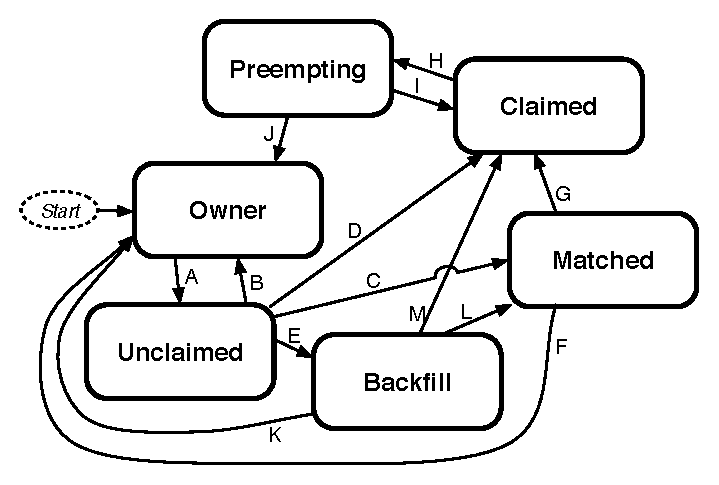
\includegraphics{admin-man/machine-states.eps}
\caption{\label{fig:machine-states}Machine States}
\end{figure}

%%%%%%%%%%%%%%%%%%%%%%%%%%%%%%%%%%%%%%%%%%%%%%%%%%%%%%%%%%%%%%%%%%%%%%
\subsection{\label{sec:Activities}
Machine Activities}
%%%%%%%%%%%%%%%%%%%%%%%%%%%%%%%%%%%%%%%%%%%%%%%%%%%%%%%%%%%%%%%%%%%%%%

Within some of these states, there could be a number of different
\Term{activities} the machine is in.  The idea is that all the things
that are true about a given state are true regardless of what activity
you are in.  However, there are certain important differences between
each activity, which is why they are separated out from each other
within a given state.  In general, you must specify both a state and
an activity to describe what ``state'' the machine is in.  This will be
denoted in this manual as ``state/activity'' pairs.  For example,
``Claimed/Busy''.  The following list describes all the possible
state/activity pairs:

\begin{itemize}

\item Owner
\begin{description}
\item[Idle] This is the only activity for Owner state.  As far as
  Condor is concerned the machine is ``Idle'' (not doing anything for
  Condor).
\end{description}

\item Unclaimed
\begin{description}
  
\item[Idle] This is the normal activity of Unclaimed machines.  The
  machine is still ``Idle'' in that the machine owner is willing to
  let someone run jobs on it, but Condor is still not using the
  machine for anything.
  
\item[Benchmarking] The machine could also be running benchmarks to
  determine the speed on this machine.  It only does this when the
  machine is in the Unclaimed state.  How often it does so is
  determined by the \Expr{RunBenchmarks} expression described below.

\end{description}

\item Matched
\begin{description}
\item[Idle] When Matched, the machine is still ``Idle'' as far as
  Condor is concerned.
\end{description}

\item Claimed
\begin{description}
  
\item[Idle] In this activity, the machine has been claimed, but the
  schedd that claimed it has yet to \Term{activate} the claim by
  requesting a \Condor{starter} to be spawned which would service a
  given job.
  
\item[Busy] Once a \Condor{starter} has been started and the claim is
  active, the machine moves to the Busy activity to signify that it's
  actually doing something as far as Condor is concerned.
  
\item[Suspended] If the job is suspended by Condor, the machine goes
  into the Suspended activity.
  The match between the schedd and machine has not been broken (the
  claim is still valid), but the job is not making any progress and
  Condor is no longer generating a load on the machine.

\end{description}

\item Preempting

  The preempting state is used for evicting a Condor job from a given
  machine.  When the machine enters the Preempting state, it checks the
  \Expr{WANT\_VACATE} expression (described below) to decide which of
  the following activities it should enter:

\begin{description}
  
\item[Vacating] Vacating simply means that the job that was running is
  in the process of checkpointing.  As soon as the checkpoint process
  completes, the machine moves into either the Owner state or the
  Claimed state, depending on why it began preempting in the first
  place.
  
\item[Killing] Killing means that the machine has requested the running
  job to exit the machine immediately, without checkpointing.

\end{description}

\end{itemize}

Figure~\ref{fig:machine-activities} on
page~\pageref{fig:machine-activities} gives the overall view of all
machine states and activities, and shows all the possible transitions
from one to another within the Condor system.  
Each transition is labeled with a number on the diagram, and
transition numbers refered to in this manual will be \Bold{bold}.  
This may seem pretty daunting, but it's actually easier to handle than
it looks.

\begin{figure}[hbt]
\centering
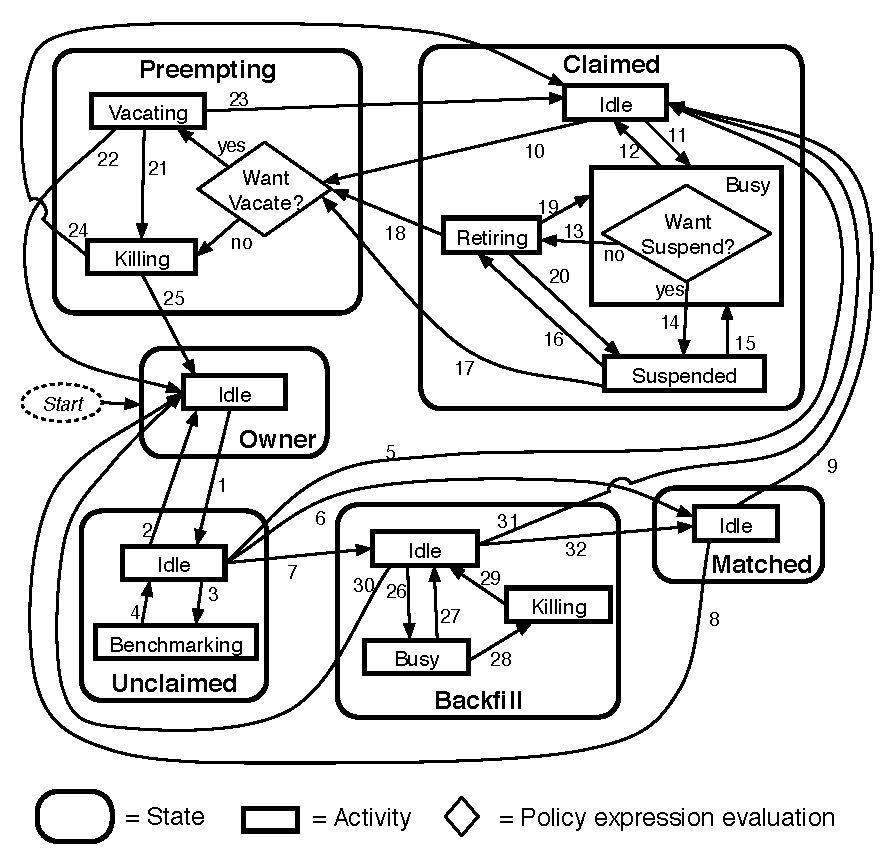
\includegraphics{admin-man/machine-activities.eps}
\caption{\label{fig:machine-activities}Machine States and Activities}
\end{figure}

Various expressions are used to determine when and if many of these
state and activity transitions occur.  Other transitions are initiated
by parts of the Condor protocol (such as when the \Condor{negotiator}
matches a machine with a schedd).  The following section describes the
conditions that lead to the various state and activity transitions.

%%%%%%%%%%%%%%%%%%%%%%%%%%%%%%%%%%%%%%%%%%%%%%%%%%%%%%%%%%%%%%%%%%%%%%
\subsection{\label{sec:State-and-Activity-Transitions}
State and Activity Transitions}
%%%%%%%%%%%%%%%%%%%%%%%%%%%%%%%%%%%%%%%%%%%%%%%%%%%%%%%%%%%%%%%%%%%%%%

This section will trace through all possible state and activity
transitions within the machine and describe the conditions under which
each one occurs.
Whenever a transition occurs, the machine records when it entered its
new activity and/or new state.
These times are often used to write the expressions that determine
when further transitions occurred (for example, you might only enter
the Killing activity if you've been in the Vacating activity longer
than a given amount of time). 

%%%%%%%%%%%%%%%%%%%%%%%%%%%%%%%%%%%%%%%%%%%%%%%%%%%%%%%%%%%%%%%%%%%%%%
\subsubsection{\label{sec:Owner-State}
Owner State}
%%%%%%%%%%%%%%%%%%%%%%%%%%%%%%%%%%%%%%%%%%%%%%%%%%%%%%%%%%%%%%%%%%%%%%

When the startd is first spawned, the machine it represents enters the
Owner state. 
The machine will remain in this state as long as the \Expr{START}
expression locally evaluates to false.
If the \Expr{START} locally evaluates to true or can't be locally
evaluated (it evaluates to \Term{undefined}), transition \Bold{1} will
occur and the machine will enter the Unclaimed state.

So long as the \Expr{START} expression locally evaluates to false,
there is no possible request in the Condor system that could match it,
so the machine in unavailable to Condor and stays in the Owner state.
For example, if the \Expr{START} expression was:
\begin{verbatim}
START : KeyboardIdle > 15 * $(MINUTE) && Owner == "coltrane" 
\end{verbatim}
and if \Attr{KeyboardIdle} was only 34 seconds, then the machine would
still be in the Owner state, even though it references Owner, which is
undefined.  \verb@False && anything@ is False, even 
\verb@False && undefined@

If, however, the \Expr{START} expression was:
\begin{verbatim}
        START : KeyboardIdle > 15 * $(MINUTE) || Owner == "coltrane"
\end{verbatim}
and \Attr{KeyboardIdle} was still only 34 seconds, then the machine
would leave the Owner state and go to Unclaimed.  This is because
``False || undefined'' is undefined.  So, while this machine isn't
available to just any body, if user ``coltrane'' has jobs submitted,
the machine is willing to run them.  Anyone else would have to wait
until \Attr{KeyboardIdle} exceeds 15 minutes.  However, since
``coltrane'' might claim this resource, but hasn't yet, the machine
goes to the Unclaimed state.

While in the Owner state the startd only polls the status of the
machine every \Macro{UPDATE\_INTERVAL} to see if anything has changed
that would lead it to a different state.  The idea is that you don't
want to put much load on the machine while the Owner is using it
(frequently waking up, computing load averages, checking the access
times on files, computing free swap space, etc), and there's nothing
time critical that the startd needs to be sure to notice as soon as it
happens.  If the \Expr{START} expression evaluates to True and it's 5
minutes before we notice it, that's a drop in the bucket of High
Throughput Computing.

The machine can only go to the Unclaimed state from the Owner state,
and only does so when the \Expr{START} expression no longer locally
evaluates to False.  Generally speaking, if the \Expr{START}
expression locally evaluates to false at any time, the machine will
either transition directly to the Owner state, or to the Preempting
state on its way to the Owner state, if there's a job running that
needs preempting.

%%%%%%%%%%%%%%%%%%%%%%%%%%%%%%%%%%%%%%%%%%%%%%%%%%%%%%%%%%%%%%%%%%%%%%
\subsubsection{\label{sec:Unclaimed-State}Unclaimed State}
%%%%%%%%%%%%%%%%%%%%%%%%%%%%%%%%%%%%%%%%%%%%%%%%%%%%%%%%%%%%%%%%%%%%%%

While in the Unclaimed state, if the \Expr{START} expression locally
evalutes to false, the machine will return to the Owner state via
transition \Bold{2}.

When it's in the Unclaimed state, another expression comes into
effect, \Expr{RunBenchmarks} \label{param:RunBenchmarks}.  
Whenever the \Expr{RunBenchmarks} evaluates to True while the machine
is in the Unclaimed state, the machine will transition from the Idle
activity to the Benchmarking activity (transition \Bold{3}) and
perform benchmarks to determine \Attr{MIPS} and \Attr{KFLOPS}.  
When the benchmarks complete, the machine returns to the Idle activity
(transition \Bold{4}).

The startd automatically inserts an attribute, \Attr{LastBenchmark},
whenever it runs benchmarks, so commonly \Attr{LastBenchmark} is
defined in terms of this attribute, for example:
\begin{verbatim}
        BenchmarkTimer = (CurrentTime - LastBenchmark)
        RunBenchmarks : $(BenchmarkTimer) >= (4 * $(HOUR))
\end{verbatim}
Here, a macro, \Macro{BenchmarkTimer} is defined to help write the
expression.  The idea is that this macro holds the time since the last
benchmark, so when this time exceeds 4 hours, we run the benchmarks
again.  The startd keeps a weighted average of these benchmarking
results to try to get the most accurate numbers possible.  That's why
you would want the startd to run them more than once in its lifetime.

\Note LastBenchmark is initialized to 0 before the benchmarks
have ever been run.
So, if you want the startd to run benchmarks as soon as the machine is
unclaimed (if it hasn't done so already), just include a term for
\Attr{LastBenchmark} as in the example above.

\Note If \Expr{RunBenchmarks} is defined, and set to something
other than ``False'', the startd will automatically run one set of
benchmarks when it first starts up.
So, if you want to totally disable benchmarks, both at startup, and at
any time thereafter, just set \Expr{RunBenchmarks} to ``False'' or
comment it out from your config file.

From the Unclaimed state, the machine can go to two other possible
states: Matched or Claimed/Idle.
Once the \Condor{negotiator} matches an Unclaimed machine with a
requester at a given schedd, the negotiator sends a command to both
parties, notifying them of the match.  
If the schedd gets that notification and initiates the claiming
procedure with the machine before the negotiator's message gets to the
machine, the Match state is skipped entirely, and the machine goes
directly to the Claimed/Idle state (transition \Bold{5}).
However, normally the machine will enter the Matched state (transition
\Bold{6}), even if it's only for a brief period of time.

%%%%%%%%%%%%%%%%%%%%%%%%%%%%%%%%%%%%%%%%%%%%%%%%%%%%%%%%%%%%%%%%%%%%%%
\subsubsection{\label{sec:Matched-State}Matched State}
%%%%%%%%%%%%%%%%%%%%%%%%%%%%%%%%%%%%%%%%%%%%%%%%%%%%%%%%%%%%%%%%%%%%%%

The Matched state is not very interesting to Condor.  The only
noteworthy things are that the machine lies about its \Expr{START}
expression while in this state and says that \Expr{Requirements} are
false to prevent being matched again before it has been claimed, and
that the startd starts a timer to make sure it doesn't stay in the
Matched state too long.  This timer is set with the
\Macro{MATCH\_TIMEOUT} \label{param:MatchTimeout} config file
parameter.  It is specified in seconds and defaults to 300 (5
minutes).  If the schedd that was matched with this machine doesn't
claim it within this period of time, the machine gives up on it, goes
back into the Owner state via transition \Bold{7} (which it will
probably leave right away to get to the Unclaimed state again, and
wait for another match). 

At any time while the machine is in the Matched state, if the
\Expr{START} expression locally evaluates to false, the machine enters
the Owner state directly (transition \Bold{7}).

If the schedd that was matched with the machine claims it before the
\Macro{MATCH\_TIMEOUT} expires, the machine goes into the Claimed/Idle
state (transition \Bold{8}).

%%%%%%%%%%%%%%%%%%%%%%%%%%%%%%%%%%%%%%%%%%%%%%%%%%%%%%%%%%%%%%%%%%%%%%
\subsubsection{Claimed State}
\label{sec:Claimed-State}
%%%%%%%%%%%%%%%%%%%%%%%%%%%%%%%%%%%%%%%%%%%%%%%%%%%%%%%%%%%%%%%%%%%%%%

The Claimed state is certainly the most complicated state.
It has the most possible activities, and the most expressions that
determine what it will do next.
In addition the \Condor{checkpoint} and \Condor{vacate} commands only
have any effect on the machine when its in the Claimed state.
In general, there are two sets of expressions that might take effect,
depending on if the universe of the request that claimed the machine is
Standard or Vanilla.
The Standard Universe expressions are the ``normal'' expressions, for
example:
\begin{verbatim}
        WANT_SUSPEND            : True
        WANT_VACATE             : $(ActivationTimer) > 10 * $(MINUTE)
        SUSPEND                 : $(KeyboardBusy) || $(CPUBusy)
        ...
\end{verbatim}

The Vanilla expressions have ``\_VANILLA'' appended to the end, for
example:
\begin{verbatim}
        WANT_SUSPEND_VANILLA    : True
        WANT_VACATE_VANILLA     : True
        SUSPEND_VANILLA         : $(KeyboardBusy) || $(CPUBusy)
        ...
\end{verbatim}

If you don't specify seperate vanilla versions, the normal versions
will be used for all jobs, including vanilla jobs.  
For the purposes of this manual, we'll always refer to the regular 
expressions.
Keep in mind that if the request was a Vanilla Universe, the Vanilla
expressions (if they were defined) would be in effect, instead.
The reason for this is that the resource owner might want the machine
to behave differently for Vanilla jobs, since they can't checkpoint.
For example, they might want to let Vanilla jobs remain suspended for
much longer than standard jobs.

While Claimed, the \Macro{POLLING\_INTERVAL} takes effect, and the
startd starts polling the machine much more frequently to evaluate its
state.

If the owner starts typing on the console again, we want to notice as
soon as possible and start doing whatever that owner wants at that
point.
For SMP machines, if any virtual machine is in the Claimed state, the
startd will poll the machine more frequently.
If we're already polling for one virtual machine, it doesn't really
cost us any more to evaluate the state of all the virtual machines at
the same time.

In general, when the startd is going to kick a job off a machine
(usually because of activity on the machine that signifies that the
owner is using the machine again) the startd will go through
successive levels of getting the job out of the way.
The first and least costly to the job is suspending it.
This even works for Vanilla jobs.
If suspending the job for a little while doesn't satisfy the machine
owner, (the owner is still using the machine after a certain period of
time, for example), the startd moves on to vacating the job, which
involves performing a checkpoint so that the work it had completed up
until this point is not lost.
If even that does not satisfy the machine owner (usually because it's
taking too long and the owner wants their machine back \emph{now}),
the final, most drastic stage is reached: killing.  
Killing is just quick death to the job, without a checkpoint.  
For Vanilla jobs, vacating and killing are basically equivalent,
though a vanilla job can request to have a certain \Term{softkill
signal} sent to it at vacate time so that it can perform
application-specific checkpointing, for example.

The \Expr{WANT\_SUSPEND} expression determines if the machine will even
evaluate the \Expr{SUSPEND} expression to consider entering the
Suspended activity.
The \Expr{WANT\_VACATE} expression determines what happens when the
machine enters the preempting state, whether it will go to the vacating
activity, or go directly to killing. 
If one or both of these expressions evaluates to false, the machine
will skip that stage of getting rid of the job and proceed directly to
the more drastic stages.

When the machine first enters the Claimed state, it goes to the Idle
activity.  From there, it has two options.  
It can enter the Preempting state via transition \Bold{9} (if a 
\Condor{vacate} comes in, or if the \Expr{START} expression locally
evaluates to false).  
Or, it can enter the busy activity (transition \Bold{10}) if the
schedd that has claimed the machine decides to activate the claim and
start a job.

From Claimed/Busy, the machine can go to many different state/activity
combinations.
The startd evaluates the \Expr{WANT\_SUSPEND} expression to decide
which other expressions to evaluate.  
If \Expr{WANT\_SUSPEND} is true, the startd will evalutate the
\Expr{SUSPEND} expression, and if it is false, the startd will
evaluate the \Expr{PREEMPT} expression and skip the Suspended activity
entirely.
Here are all the possibile state/activity destinations that the
machine can get to from Claimed/Busy:

\begin{description}
  
\item[Claimed/Idle] If the starter that is serving a given job exits
  (because the jobs completes, for example), the machine will go back
  to Claimed/Idle (transition \Bold{11}).
  
\item[Preempting] If \Expr{WANT\_SUSPEND} is false and the
  \Expr{PREEMPT} expression is true, the machine will enter the
  Preempting state (transition \Bold{12}).
  
\item[Claimed/Suspended] If both the \Expr{WANT\_SUSPEND} and
  \Expr{SUSPEND} expressions evaluate to true, the machine will
  suspend the job (transition \Bold{13}).
  
  The other reason the machine would go from Claimed/Busy to
  Preempting is if the \Condor{negotiator} matched the machine
  with a ``better'' match.  This better match could either be from the
  machine's perspective (see section~\ref{sec:Rank-Expression} on the
  \Expr{RANK} Expression above) or from the negotiator's perspective
  (because a user with a better user priority has jobs that should be
  running on this machine).
  In this case, \Expr{WANT\_VACATE} is assumed to be true, and the
  machine will always go to Preempting/Vacating.
  
\item[Claimed/Busy] While it's not really a state change, there is
  another thing that could happen to the machine while it's in
  Claimed/Busy, which is that either a \Condor{checkpoint} command
  could arrive, or the \Expr{PeriodicCheckpoint} expression could
  evaluate to true.  When either of these things occur, the startd
  requests that the job begin a periodic checkpoint.  Since the startd
  has no way to know when this process completes, there's no way
  periodic checkpointing could be its own state.  However, for the
  purposes of all the expressions, periodic checkpointing is
  Claimed/Busy, just like a job was running.

\end{description}

You already know what happens in Claimed/Idle, so now we'll discuss
what happens in Claimed/Suspended.  Again, there are multiple
state/activity combinations that you can reach from Claimed/Suspended:

\begin{description}
  
\item[Claimed/Busy] If the \Expr{CONTINUE} expression evaluates to
  true, the machine will resume the computation and will go back to the
  Claimed/Busy state (transition \Bold{14}).

\item[Preempting] If the \Expr{PREEMPT} expression is true, the machine
  will enter the Preempting state (transition \Bold{15}).

\end{description}

From the Claimed state, you can only enter other activities in the
Claimed state (all of which we've already discussed), or the
Preempting state, which is described next.

%%%%%%%%%%%%%%%%%%%%%%%%%%%%%%%%%%%%%%%%%%%%%%%%%%%%%%%%%%%%%%%%%%%%%%
\subsubsection{\label{sec:Preempting-State}Preempting State}
%%%%%%%%%%%%%%%%%%%%%%%%%%%%%%%%%%%%%%%%%%%%%%%%%%%%%%%%%%%%%%%%%%%%%%

The Preempting state is much less complicated than the Claimed state.
Basically, there are two possible activities, and two possible
destinations.  Depending on \Expr{WANT\_VACATE} you either enter the
Vacating activity (if it's true) or the Killing activity (if it's
false).  

While in the Preempting state (regardless of activity) the machine
advertises its \Expr{Requirements} expression as False to signify that
it is not available for further matches, either because it is about to go
to the owner state anyway, or because it has already been matched with
one preempting match, and further preempting matches are disallowed
until the machine has been claimed by the new match.

The main function of the Preempting state is to get rid of the starter
associated with this resource.  If the \Condor{starter} associated
with a given claim exits while the machine is still in the Vacating
activity, it means the job successfully completed its checkpoint.

If the machine is in the Vacating activity, it keeps evaluating the 
\Expr{KILL} expression.  As soon as this expression evaluates to true,
the machine enters the Killing activity (transition \Bold{16}).

When the starter exits, or if there was no starter running when the
machine enters the Preempting state (because it came from
Claimed/Idle), the other job of the preempting state is completed:
notifying the schedd that had claimed this machine that the claim is
broken.

At this point, the machine will either enter the Owner state via
transition \Bold{17} (if the job was preempted because the machine
owner came back) or the Claimed/Idle state via transition \Bold{18}
(if the job was preempted because a better match was found).

Then the machine enters the Killing activity, it begins a timer, the
length of which is defined by the \Macro{KILLING\_TIMEOUT}
\label{param:KillingTimeout} macro.  This macro is defined in seconds 
and defaults to 30.  If this timer expires and the machine is still in
the Killing activity, something has gone seriously wrong with the
\Condor{starter} and the startd tries to vacate the job immediately by
sending SIGKILL to all of the \Condor{starter}'s children, and then to
the \Condor{starter} itself.

Again, once the starter is gone and the schedd that had claimed the
machine is notified that the claim is broken, the machine will either
enter the Owner state via transition \Bold{19} (if the job was
preempted because the machine owner came back) or the Claimed/Idle
state via transition \Bold{20} (if the job was preempted because a
better match was found). 

%%%%%%%%%%%%%%%%%%%%%%%%%%%%%%%%%%%%%%%%%%%%%%%%%%%%%%%%%%%%%%%%%%%%%%
\subsection{\label{sec:State-Expression-Summary}
State/Activity Transition Expression Summary}
%%%%%%%%%%%%%%%%%%%%%%%%%%%%%%%%%%%%%%%%%%%%%%%%%%%%%%%%%%%%%%%%%%%%%%
The following section is meant to summarize the information from the
previous sections to serve as a quick reference.  If anything is
unclear here, please refer to the previous sections for clarification.

\begin{description}
  
\item[\Expr{START}] When this is true, the machine is willing to spawn
  a remote Condor job.
  
\item[\Expr{RunBenchmarks}] While in the Unclaimed state, the machine
  will run benchmarks whenever this is true.
  
\item[\Macro{MATCH\_TIMEOUT}] If the machine has been in the Matched
  state longer than this, it will go back to the Owner state.
  
\item[\Expr{WANT\_SUSPEND}] If this is true, the machine will evaluate
  the \Expr{SUSPEND} expression to see if it should transition to the
  Suspended activity.  If this is false, the machine will look at
  the \Expr{PREEMPT} expression.
  
\item[\Expr{SUSPEND}] If \Expr{WANT\_SUSPEND} is true, and the machine
  is in the Claimed/Busy state, it will enter the Suspended activity
  if \Expr{SUSPEND} is true.
  
\item[\Expr{CONTINUE}] If the machine is in the Claimed/Suspended
  state, it will enter the Busy activity if \Expr{CONTINUE} is true.
  
\item[\Expr{PREEMPT}] If the machine is either in the Claimed/Suspended
  activity, or is in the Claimed/Busy activity and the
  \Expr{WANT\_SUSPEND} is false, the machine will enter the Preempting
  state whenever \Expr{PREEMPT} is true. 
  
\item[\Expr{WANT\_VACATE}] This is only checked when the
  \Expr{PREEMPT} expression is true and the machine enters the
  Preempting state.
  If \Expr{WANT\_VACATE} is true, the machine will enter the Vacating
  activity.  
  If it is false, the machine will proceed directly to the Killing
  activity.  
  
\item[\Expr{KILL}] If the machine is the Preempting/Vacating state, it
  will enter Preempting/Killing whenever \Expr{KILL} is true. 
  
\item[\Macro{KILLING\_TIMEOUT}] If the machine is in the
  Preempting/Killing state for longer than \Macro{KILLING\_TIMEOUT}
  seconds, the startd will just send a SIGKILL to the \Condor{starter}
  and all its children to try to kill the job as quickly as possible.
  
\item[\Expr{PERIODIC\_CHECKPOINT}] If the machine is in the
  Claimed/Busy state and \Expr{PERIODIC\_CHECKPOINT} is true, the
  user's job will begin a periodic checkpoint.
  
\item[\Expr{RANK}] If this expression evaluates to a higher number for
  a pending resource request than it does for the current request, the
  machine will preempt the current request (enter the
  Preempting/Vacating state).  When the preemption is complete, the
  machine will enter the Claimed/Idle state with the new resource
  request claiming it.

\end{description}

%%%%%%%%%%%%%%%%%%%%%%%%%%%%%%%%%%%%%%%%%%%%%%%%%%%%%%%%%%%%%%%%%%%%%%
\subsection{\label{sec:Example-Policy}Example Policy Settings}
%%%%%%%%%%%%%%%%%%%%%%%%%%%%%%%%%%%%%%%%%%%%%%%%%%%%%%%%%%%%%%%%%%%%%%

The following section provides two examples of how you might configure
the policy at your pool.  Each one is described in English, then the
actual macros and expressions used are listed and explained with
comments.  Finally the entire set of macros and expressions are listed
in one block so you can see them in one place for easy reference.

%%%%%%%%%%%%%%%%%%%%%%%%%%%%%%%%%%%%%%%%%%%%%%%%%%%%%%%%%%%%%%%%%%%%%%
\subsubsection{\label{sec:Default-Policy}Default Policy Settings}
%%%%%%%%%%%%%%%%%%%%%%%%%%%%%%%%%%%%%%%%%%%%%%%%%%%%%%%%%%%%%%%%%%%%%%

These settings are the default as shipped with Condor.  They have been
used for many years with no problems.  The Vanilla expressions are
identical to the regular ones. (They aren't even listed here.  If you
don't define them, the regular expressions are used for Vanilla jobs
as well).

First, we define a bunch of macros which help us write the expressions
more clearly.  In particular, we use:

\begin{description}
  
\item[\Macro{StateTimer}] How long we've been in the current state.

\item[\Macro{ActivityTimer}] How long we've been in the current
  activity. 

\item[\Macro{ActivationTimer}] How long the has job been running on
  this machine.

\item[\Macro{LastCkpt}] How long it's been since we last performed a
  periodic checkpoint.

\item[\Macro{NonCondorLoadAvg}] The difference of the system load and
  the Condor load (i.e the load generated by everything but Condor).

\item[\Macro{BackgroundLoad}] How much background load we're willing
  to have on our machine and still start a Condor job.

\item[\Macro{BackgroundLoad}] How much background load we're willing
  to have on our machine and still start a Condor job.

\item[\Macro{HighLoad}] If the \MacroU{NonCondorLoadAvg} goes over
  this, the CPU is ``busy'' and we want to start evicting the Condor
  job. 

\item[\Macro{StartIdleTime}] How long the keyboard has to be idle
  before we'll start a job.

\item[\Macro{ContinueIdleTime}] How long the keyboard has to be idle
  before we'll resume a suspended job.

\item[\Macro{MaxSuspendTime}] How long we're willing to let the job be
  suspended before we move on to more drastic measures.

\item[\Macro{MaxVacateTime}] How long we're willing to let the job be
  checkpointing before we give up on it and have to kill it outright.

\item[\Macro{KeyboardBusy}] A boolean string that evaluates to true
    when the keyboard is being used. 

\item[\Macro{CPU\_Idle}] A boolean string that evaluates to true
    when the CPU is idle is being used.

\item[\Macro{CPU\_Busy}] A boolean string that evaluates to true
    when the CPU is busy.

\item[\Macro{MachineBusy}] The CPU or the Keyboard is busy.

\end{description}

\begin{verbatim}
##  These macros are here to help write legible expressions:
MINUTE          = 60
HOUR            = (60 * $(MINUTE))
StateTimer      = (CurrentTime - EnteredCurrentState)
ActivityTimer   = (CurrentTime - EnteredCurrentActivity)
ActivationTimer = (CurrentTime - JobStart)

NonCondorLoadAvg        = (LoadAvg - CondorLoadAvg)
BackgroundLoad          = 0.3
HighLoad                = 0.5
StartIdleTime           = 15 * $(MINUTE)
ContinueIdleTime        = 5 * $(MINUTE)
MaxSuspendTime          = 10 * $(MINUTE)
MaxVacateTime           = 5 * $(MINUTE)

KeyboardBusy            = KeyboardIdle < $(MINUTE)
CPU_Idle                = $(NonCondorLoadAvg) <= $(BackgroundLoad)
CPU_Busy                = $(NonCondorLoadAvg) >= $(HighLoad)
MachineBusy             = ($(CPU_Busy) || $(KeyboardBusy))
\end{verbatim}

Now, we define that we always want to suspend jobs.
If that's not enough, we'll always try to gracefully vacate them,
unless they've only been running for less than 10 minutes anyway, in
which case we'll just kill them, instead of trying to checkpoint those
10 minutes of work.
\begin{verbatim}
WANT_SUSPEND            : True
WANT_VACATE             : $(ActivationTimer) > 10 * $(MINUTE)
\end{verbatim}

Finally, we define the actual expressions.  Start any job if the CPU
is idle (as defined by our macro), and the keyboard has been idle long
enough.
\begin{verbatim}
START           : $(CPU_Idle) && KeyboardIdle > $(StartIdleTime)
\end{verbatim}

Suspend a job if the machine is busy.
\begin{verbatim}
SUSPEND         : $(MachineBusy)
\end{verbatim}

Continue a suspended job if the CPU is idle and the Keyboard has been
idle for long enough.
\begin{verbatim}
CONTINUE        : $(CPU_Idle) && KeyboardIdle > $(ContinueIdleTime)
\end{verbatim}

There are two conditions that we want to preempt under.
First, if we have suspended the job, but it's been suspended too long.
Second, if we don't even want to suspend the job, and the machine is
busy. 
\begin{verbatim}
PREEMPT	        : ( ($(ActivityTimer) > $(MaxSuspendTime)) && \
                   (Activity == "Suspended") ) || \
                  ( $(MachineBusy) && (WANT_SUSPEND == False) )
\end{verbatim}

Kill a job if we've been vacating for too long.
\begin{verbatim}
KILL            : $(ActivityTimer) > $(MaxVacateTime)
\end{verbatim}

Finally, specify we want periodic checkpointing.  
For jobs smaller than 60 megs, we periodic checkpoint every 6 hours.  
For larger jobs, we only checkpoint every 12 hours.
\begin{verbatim}
PERIODIC_CHECKPOINT     : ( (ImageSize < 60000) && \
                            ($(LastCkpt) > (6 * $(HOUR))) ) || \ 
                          ( $(LastCkpt) > (12 * $(HOUR)) )
\end{verbatim}

For clarity and reference, the entire set policy settings are included
once more without comments:

\begin{verbatim}
##  These macros are here to help write legible expressions:
MINUTE          = 60
HOUR            = (60 * $(MINUTE))
StateTimer      = (CurrentTime - EnteredCurrentState)
ActivityTimer   = (CurrentTime - EnteredCurrentActivity)
ActivationTimer = (CurrentTime - JobStart)
LastCkpt	= (CurrentTime - LastPeriodicCheckpoint)

NonCondorLoadAvg        = (LoadAvg - CondorLoadAvg)
BackgroundLoad          = 0.3
HighLoad                = 0.5
StartIdleTime           = 15 * $(MINUTE)
ContinueIdleTime        = 5 * $(MINUTE)
MaxSuspendTime          = 10 * $(MINUTE)
MaxVacateTime           = 5 * $(MINUTE)

KeyboardBusy            = KeyboardIdle < $(MINUTE)
CPU_Idle                = $(NonCondorLoadAvg) <= $(BackgroundLoad)
CPU_Busy                = $(NonCondorLoadAvg) >= $(HighLoad)
MachineBusy             = ($(CPU_Busy) || $(KeyboardBusy))

WANT_SUSPEND            : True
WANT_VACATE             : $(ActivationTimer) > 10 * $(MINUTE)

START           : $(CPU_Idle) && KeyboardIdle > $(StartIdleTime)
SUSPEND         : $(MachineBusy)
CONTINUE        : $(CPU_Idle) && KeyboardIdle > $(ContinueIdleTime)
PREEMPT	        : ( ($(ActivityTimer) > $(MaxSuspendTime)) && \
                   (Activity == "Suspended") ) || \
                  ( $(MachineBusy) && (WANT_SUSPEND == False) )
KILL            : $(ActivityTimer) > $(MaxVacateTime)

PERIODIC_CHECKPOINT     : ( (ImageSize < 60000) && \
                            ($(LastCkpt) > (6 * $(HOUR))) ) || \ 
                          ( $(LastCkpt) > (12 * $(HOUR)) )
\end{verbatim}

%%%%%%%%%%%%%%%%%%%%%%%%%%%%%%%%%%%%%%%%%%%%%%%%%%%%%%%%%%%%%%%%%%%%%%
\subsubsection{\label{sec:UW-Policy}
UW-Madison CS Condor Pool Policy Settings} 
%%%%%%%%%%%%%%%%%%%%%%%%%%%%%%%%%%%%%%%%%%%%%%%%%%%%%%%%%%%%%%%%%%%%%%

Due to a recent increase in the number of Condor users and the size of
their jobs (many users here are submitting jobs with an
\Attr{Imagesize} of over 100 megs!), we have had to customize our
policy to try to handle this range of \Attr{Imagesize} better.

Basically, whether or not we suspend or vacate jobs is now a function
of the \Attr{Imagesize} of the job that's currently running (which is
defined in terms of kilobytes).  We have divided the \Attr{Imagesize}
into three possible categories, which we define with macros.
\begin{verbatim}
BigJob          = (ImageSize > (30 * 1024))
MediumJob       = (ImageSize <= (30 * 1024) && ImageSize >= (10 * 1024))
SmallJob        = (ImageSize < (10 * 1024))
\end{verbatim}

Our policy can be summed up with the following few sentences: If the
job is ``small'', it goes through the normal progression of suspend to
vacate to kill based on the tried and true times.  If the job is
``medium'', when the user comes back, we start vacating the job right
away.  The idea is that if we checkpoint immediately, all our pages
are still in memory, checkpointing will be fast, and we'll free up
memory pages as soon as we checkpoint.  If we suspend, our pages will
start getting swapped out and when we finally want to checkpoint (10
minutes later), we'll have to start swapping out the user's pages
again, they'll see reduced performance, and checkpointing will take
much longer.  If the job is ``big'', don't even bother checkpointing,
since we won't finish before the owner gets too upset and we might as
well not even bother putting the wasted load on the network and
checkpoint server.

All the logic for our pool's special policy is tuned with the
\Expr{WANT\_\*} expressions. 
All of the other expressions and macros just use the defaults.
We only want to suspend jobs if they are ``small'', and we only want
to vacate jobs that are ``small'' or ``medium''.  
We still want to always suspend Vanilla jobs, regardless of their
size.
\begin{verbatim}
WANT_SUSPEND            : $(SmallJob)
WANT_VACATE             : $(MediumJob) || $(SmallJob)
WANT_SUSPEND_VANILLA    : True
WANT_VACATE_VANILLA     : True
\end{verbatim}

Now, we define the actual expressions, (which we just use the defaults
for).
We really do this with macros and simply define the expressions with
the macros later on.
This may seem really strange, but we do it because it makes it easier
to do special customized settings (for example, for testing purposes)
and still reference the defaults.
There will be a brief example of this at the end of this section.
\begin{verbatim}
CS_START        = $(CPU_Idle) && KeyboardIdle > $(StartIdleTime)
CS_SUSPEND      = $(MachineBusy)
CS_CONTINUE     = (KeyboardIdle > $(ContinueIdleTime)) && $(CPU_Idle)
CS_PREEMPT      = ( ($(ActivityTimer) > $(MaxSuspendTime)) && \
                   (Activity == "Suspended") ) || \
                  ( $(MachineBusy) && (WANT_SUSPEND == False) )
CS_KILL         = ($(ActivityTimer) > $(MaxVacateTime))
\end{verbatim}

Here's where we actually define the expressions in terms of our
special macros:
\begin{verbatim}
START       : $(CS_START)
SUSPEND     : $(CS_SUSPEND)
CONTINUE    : $(CS_CONTINUE)
PREEMPT     : $(CS_PREEMPT)
KILL        : $(CS_KILL)
\end{verbatim}

We still don't want to define seperate Vanilla versions of any of
these, since we already have a different \Expr{WANT\_SUSPEND} for
vanilla jobs and all of the policy expressions are just written in
terms of that. 

Periodic checkpointing also takes image size into account.  
Since we kill large jobs right away at eviction time, we want to
periodically checkpoint them more frequently (every 3 hours), since
that's the only way they make forward progress.
However, with all those large periodic checkpoints going on on so
frequently, we don't want to bog down our network or our checkpoint
servers.
So, we only periodic checkpoint small or medium jobs every 12 hours,
since they get the privilege of checkpointing at eviction time.
\begin{verbatim}
PERIODIC_CHECKPOINT  : (($(LastCkpt) > (3 * $(HOUR))) \
      && $(BigJob)) || (($(LastCkpt) > (12 * $(HOUR))) && \
      ($(SmallJob) || $(MediumJob)))
\end{verbatim}

For clarity and reference, the entire set of policy settings are
included once more, without comments:
\begin{verbatim}
ActivationTimer = (CurrentTime - JobStart)
StateTimer      = (CurrentTime - EnteredCurrentState)
ActivityTimer   = (CurrentTime - EnteredCurrentActivity)
LastCkpt        = (CurrentTime - LastPeriodicCheckpoint)

NonCondorLoadAvg   = (LoadAvg - CondorLoadAvg)
BackgroundLoad     = 0.3
HighLoad           = 0.5
StartIdleTime      = 15 * $(MINUTE)
ContinueIdleTime   = 5 * $(MINUTE)
MaxSuspendTime     = 10 * $(MINUTE)
MaxVacateTime      = 5 * $(MINUTE)

KeyboardBusy       = KeyboardIdle < $(MINUTE)
CPU_Idle           = $(NonCondorLoadAvg) <= $(BackgroundLoad)
CPU_Busy           = $(NonCondorLoadAvg) >= $(HighLoad)
MachineBusy        = ($(CPU_Busy) || $(KeyboardBusy))

BigJob       = (ImageSize > (30 * 1024))
MediumJob    = (ImageSize <= (30 * 1024) && ImageSize >= (10 * 1024))
SmallJob     = (ImageSize < (10 * 1024))

WANT_SUSPEND            : $(SmallJob)
WANT_VACATE             : $(MediumJob) || $(SmallJob)
WANT_SUSPEND_VANILLA    : True
WANT_VACATE_VANILLA     : True

CS_START    = $(CPU_Idle) && KeyboardIdle > $(StartIdleTime)
CS_SUSPEND  = $(CPU_Busy) || $(KeyboardBusy)
CS_CONTINUE = (KeyboardIdle > $(ContinueIdleTime)) && $(CPU_Idle)
CS_PREEMPT  = ( ($(ActivityTimer) > $(MaxSuspendTime)) && \
               (Activity == "Suspended") ) || \
              ( $(MachineBusy) && (WANT_SUSPEND == False) )
CS_KILL     = ($(ActivityTimer) > $(MaxVacateTime))

START       : $(CS_START)
SUSPEND     : $(CS_SUSPEND)
CONTINUE    : $(CS_CONTINUE)
PREEMPT     : $(CS_PREEMPT)
KILL        : $(CS_KILL)

PERIODIC_CHECKPOINT  : (($(LastCkpt) > (3 * $(HOUR))) \
      && $(BigJob)) || (($(LastCkpt) > (12 * $(HOUR))) && \
      ($(SmallJob) || $(MediumJob)))
\end{verbatim}

As a final example, we show how our default macros can be used to
setup a given machine for testing.  Suppose we want the machine to
behave just like normal, but if user ``coltrane'' submits a job, we
want that job to start regardless of what's happening on the machine,
and we don't want the job suspended, vacated or killed.  For example,
we might know ``coltrane'' is just going to be submitting very short
running programs to test something and he wants to see them execute
right away.  Anyway, we could configure any machine (or our whole
pool, for that matter) with the following 5 expressions:
\begin{verbatim}
        START      : ($(CS_START)) || Owner == "coltrane"
        SUSPEND    : ($(CS_SUSPEND)) && Owner != "coltrane"
        CONTINUE   : $(CS_CONTINUE)
        PREEMPT    : ($(CS_PREEMPT)) && Owner != "coltrane"
        KILL       : $(CS_KILL)
\end{verbatim}
Notice that you don't have to do anything special with either the
\Expr{CONTINUE} or \Expr{KILL} expressions.
If Coltrane's jobs never suspend, they'll never even look at
\Expr{CONTINE}.  
Similarly, if they never preempt, they'll never look at \Expr{KILL}. 

%%%%%%%%%%%%%%%%%%%%%%%%%%%%%%%%%%%%%%%%%%%%%%%%%%%%%%%%%%%%%%%%%%%%%%%%%%%
\section{\label{sec:Security}Security In Condor}
%%%%%%%%%%%%%%%%%%%%%%%%%%%%%%%%%%%%%%%%%%%%%%%%%%%%%%%%%%%%%%%%%%%%%%%%%%%

This section describes various aspects of security within Condor.
The section is not yet complete.

%%%%%%%%%%%%%%%%%%%%%%%%%%%%%%%%%%%%%%%%%%%%%%%%%%%%%%%%%%%%%%%%%%%%%%
\subsection{\label{sec:Non-Root}Running Condor as Non-Root}
%%%%%%%%%%%%%%%%%%%%%%%%%%%%%%%%%%%%%%%%%%%%%%%%%%%%%%%%%%%%%%%%%%%%%%

While we strongly recommend starting up the Condor daemons as root, we
understand that it is not always possible.
The main problems appear
if you have one Condor installation shared by many users
on a single machine, or if you are setting up machines to only
execute Condor jobs.
If you are setting up a submit-only installation for
a single user, then there is no need for (or benefit from) running as
root.  

What follows are the effects on the various parts of Condor
of running without root access.

\begin{description}

\item[\Condor{startd}] If you're setting up a machine to run Condor
   jobs and don't start the \Condor{startd} as root, you're basically
   relying on the goodwill of your Condor users to agree to the policy
   you configure the startd to enforce as far as starting, suspending,
   vacating and killing Condor jobs under certain conditions.  If you
   run as root, however, you can enforce these policies regardless of
   malicious users.  By running as root, the Condor daemons run with a
   different UID than the Condor job that gets started (since the
   user's job is started as either the UID of the user who submitted
   it, or as user ``nobody'', depending on the \Macro{UID\_DOMAIN}
   settings).  Therefore, the Condor job cannot do anything to the
   Condor daemons.  If you don't start the daemons as root, all
   processes started by Condor, including the end user's job, run with
   the same UID (since you can't switch UIDs unless you're root).
   Therefore, a user's job could just kill the \Condor{startd} and
   \Condor{starter} as soon as it starts up and by doing so, avoid
   getting suspended or vacated when a user comes back to the machine.
   This is nice for the user, since they get unlimited access to the
   machine, but awful for the machine owner or administrator.  If you
   trust the users submitting jobs to Condor, this might not be a
   concern.  However, to ensure that the policy you choose is
   effectively enforced by Condor, the \Condor{startd} should be
   started as root.

   In addition, some system information cannot be obtained without
   root access on some platforms (such as load average on IRIX).  As a
   result, when we're running without root access, the startd has to
   call other programs (for example, ``uptime'') to get this
   information.  This is much less efficient than getting the
   information directly from the kernel (which is what we do if we're
   running as root).  On Linux and Solaris, we can get this
   information directly without root access, so this is not a concern
   on those platforms.

   If you can't have all of Condor running as root, at least consider
   whether you can install the Condor{startd} as setuid root.  That
   would solve both of these problems.  If you can't do that, you
   could also install it as a setgid sys or kmem program (depending on
   whatever group has read access to \File{/dev/kmem} on your system)
   and that would at least solve the system information problem.

\item[\Condor{schedd}] The biggest problem running the schedd
    without root access is that the \Condor{shadow} processes which it
    spawns are stuck with the same UID the \Condor{schedd} has.  This
    means that users submitting their jobs have to go out of their way
    to grant write access to user or group condor (or whoever the
    schedd is running as) for any files or directories their jobs
    write or create.  Similarly, read access must be granted to their
    input files.

    You might consider installing \Condor{submit} as a setgid condor
    program so that at least the \File{stdout}, \File{stderr} and
    \File{UserLog} files get created with the right permissions.  If
    \Condor{submit} is a setgid program, it will automatically set
    it's umask to 002, so that creates group-writable files.  This
    way, the simple case of a job that just writes to \File{stdout}
    and \File{stderr} will work.  If users have programs that open
    their own files, they'll have to know to set the right permissions
    on the directories they submit from.

\item[\Condor{master}] The \Condor{master} is what spawns the
    \Condor{startd} and \Condor{schedd}, so if want them both running
    as root, you should have the master run as root.  This happens
    automatically if you start the master from your boot scripts.

\item[\Condor{negotiator}]
\item[\Condor{collector}] There is no need to have either of these
daemons running as root.

\item[\Condor{kbdd}] On platforms that need the \Condor{kbdd} (Digital
    Unix and IRIX) the \Condor{kbdd} has to run as root.  If it is
    started as any other user, it will not work.  You might consider
    installing this program as a setuid root binary if you can't run
    the \Condor{master} as root.  Without the \Condor{kbdd}, the
    startd has no way to monitor mouse activity at all, and the only
    keyboard activity it will notice is activity on ttys (such as
    xterms, remote logins, etc).

\end{description}

%%%%%%%%%%%%%%%%%%%%%%%%%%%%%%%%%%%%%%%%%%%%%%%%%%%%%%%%%%%%%%%%%%%%%%
\subsection{\label{sec:uids}UIDs in Condor}
%%%%%%%%%%%%%%%%%%%%%%%%%%%%%%%%%%%%%%%%%%%%%%%%%%%%%%%%%%%%%%%%%%%%%%
\Todo

%%%%%%%%%%%%%%%%%%%%%%%%%%%%%%%%%%%%%%%%%%%%%%%%%%%%%%%%%%%%%%%%%%%%%%
\subsection{\label{sec:Config-Security} Security through Configuration}
%%%%%%%%%%%%%%%%%%%%%%%%%%%%%%%%%%%%%%%%%%%%%%%%%%%%%%%%%%%%%%%%%%%%%%

Condor adds strong authentication and encryption to its network
communications.
Most of these security features are not visible to the user
(one who submits jobs).
They are enabled through the use of configuration macros.
The macros describe the authentication, encryption, and
integrity assurance used by various portions of Condor in its communications.

Authentication provides an assurance of the identity of one of the
communicating parties.
Mutual authentication provides an assurance of the identities of
both of the communicating parties.
Encoding information such that its contents is hidden from outsiders
is called encryption.
The integrity of a message is assured when any form of
tampering with an encrypted message can be detected. 
Nothing can be added, deleted, or modified.

When Condor is installed, default configuration settings
use no authentication or encryption.
This allows newer versions of Condor with macros
that enable secure communications to work or interact
with previous versions that had no security.
An administrator must modify the configuration settings to
enable the security features.

Inside Condor, daemons or tools or user-issued commands
require communication with a Condor daemon.
It is the communication that can be made more secure.
The sender is also called a client.
Based on the configuration settings,
these communications can require authentication, encryption,
and integrity checks.

The messages are requests that include
a specification of the functionality required,
together with any of the sender's (client's) information with
respect to secure communication.
For each type of request, there is a predefined access level
required for the request to be completed.

When a daemon receives a request,
it uses a combination of the client's security information
(included with the request)
together with its own configuration settings to decide upon
the security aspects of the communication.
This can be considered a negotiation between the sender and
the daemon.
The daemon replies to the client with a confirmation of
the security aspects of the communication.
If this includes a required authentication, then the
client must follow the chosen protocol.

After a required authentication, the client can again send its
request to the daemon. 
The daemon identifies the access level required for the specific
request,
and it checks the configuration settings to determine if the client 
has the required access level.
If the client has the required access level,
permission is granted, and the request is filled. 

%%%%%%%%%%%%%%%%%%%%%%%%%%%%%%%%%%%%%%%%%%%%%%%%%%%%%%%%%%%%%%%%%%%%%%
\subsubsection{\label{sec:Security-access-levels} Access Level Descriptions}
%%%%%%%%%%%%%%%%%%%%%%%%%%%%%%%%%%%%%%%%%%%%%%%%%%%%%%%%%%%%%%%%%%%%%%
The following enumerate and describe the various access levels.
The list is hierarchical, although two extra levels are
not included in the hierarchy.
This list is given in order, with the level of lowest ability first.

\begin{description}

% editted
\item[\DCPerm{READ}] \label{dcperm:read} \DCPerm{READ} level
   access can obtain or read information about Condor.
   Examples that require only \DCPerm{READ} access are
   viewing the status of the pool, seeing the job queue(s),
   or viewing user permissions.
   \DCPerm{READ} access does not allow any
   changes, and it does not allow job submission.

% needs an example
\item[\DCPerm{WRITE}] \label{dcperm:write} \DCPerm{WRITE} access
   is required to send (write) information to Condor.
   Note that \DCPerm{WRITE} access does not include \DCPerm{READ} access.
   They are separate access levels.
   %Most notably, a machine can join a pool by sending ClassAd
   %updates to the central manager. 
   %The machine can talk to the other machines
   %in a pool in order to submit or run jobs.
   %In addition, any machine with
   %\DCPerm{WRITE} access can request the \Condor{startd} daemon to perform a
   %periodic checkpoint on a currently executing job. After a
   %periodic checkpoint, the job will continue to execute, and the
   %machine will still be claimed by whatever \Condor{schedd} daemon had claimed it.
   %This allows users on the machines where they submitted their jobs

\item[\DCPerm{ADMINISTRATOR}] \label{dcperm:administrator} The
   \DCPerm{ADMINISTRATOR} access level has additional Condor
   administrator rights to the pool.  This includes the ability to
   change user priorities (with the command \Condor{userprio -set}),
   and the ability to turn Condor on and off
   (as with the command \Condor{off}).

\item[\DCPerm{CONFIG}] \label{dcperm:config} This access level is
   required to modify a daemon's configuration using
   the \Condor{config\_val} command.
   By default, this level of access is allowed
   to change any configuration parameters, except those specified in
   the \File{condor\_config.root} configuration file.

\item[\DCPerm{DAEMON}] \label{dcperm:config} 

\end{description}

The two access levels that are not included in the hierarchy:
\begin{description}
% editted
\item[\DCPerm{OWNER}] \label{dcperm:owner} This level of access is
   required for commands that the owner of a machine (any local user)
   should be able to use, in addition to the Condor administrators.
   An example that requires the \DCPerm{OWNER} access level is
   the \Condor{vacate} command.
   The command causes the \Condor{startd} daemon to vacate any
   Condor job currently running on a machine.
   The owner of that machine should be able to cause the removal
   of a job running on the machine.

\item[\DCPerm{NEGOTIATOR}] \label{dcperm:negotiator} This 
   access level is used specifically to verify that commands are
   sent by the \Condor{negotiator} daemon.
   The \Condor{negotiator} daemon runs on the central manager of
   the pool.
   Commands requiring this access
   level are the ones that tell the \Condor{schedd} daemon to begin
   negotiating, and those that tell an available \Condor{startd} daemon
   that it has been matched to a \Condor{schedd} with jobs to run.

\end{description}

%%%%%%%%%%%%%%%%%%%%%%%%%%%%%%%%%%%%%%%%%%%%%%%%%%%%%%%%%%%%%%%%%%%%%%
\subsubsection{\label{sec:Security-macros} Security Configuration Macro Definitions}
%%%%%%%%%%%%%%%%%%%%%%%%%%%%%%%%%%%%%%%%%%%%%%%%%%%%%%%%%%%%%%%%%%%%%%

% server-side 
\index{configuration macro!SEC\_DEFAULT\_AUTHENTICATION@\texttt{SEC\_DEFAULT\_AUTHENTICATION}}
\index{configuration macro!SEC\_DEFAULT\_ENCRYPTION@\texttt{SEC\_DEFAULT\_ENCRYPTION}}
\index{configuration macro!SEC\_DEFAULT\_INTEGRITY@\texttt{SEC\_DEFAULT\_INTEGRITY}}
%\index{configuration macro!SEC\_DEFAULT\_NEGOTIATION@\texttt{SEC\_DEFAULT\_NEGOTIATION}}
\index{configuration macro!SEC\_READ\_AUTHENTICATION@\texttt{SEC\_READ\_AUTHENTICATION}}
\index{configuration macro!SEC\_READ\_ENCRYPTION@\texttt{SEC\_READ\_ENCRYPTION}}
\index{configuration macro!SEC\_READ\_INTEGRITY@\texttt{SEC\_READ\_INTEGRITY}}
%\index{configuration macro!SEC\_READ\_NEGOTIATION@\texttt{SEC\_READ\_NEGOTIATION}}
\index{configuration macro!SEC\_WRITE\_AUTHENTICATION@\texttt{SEC\_WRITE\_AUTHENTICATION}}
\index{configuration macro!SEC\_WRITE\_ENCRYPTION@\texttt{SEC\_WRITE\_ENCRYPTION}}
\index{configuration macro!SEC\_WRITE\_INTEGRITY@\texttt{SEC\_WRITE\_INTEGRITY}}
%\index{configuration macro!SEC\_WRITE\_NEGOTIATION@\texttt{SEC\_WRITE\_NEGOTIATION}}
\index{configuration macro!SEC\_ADMIN\_AUTHENTICATION@\texttt{SEC\_ADMIN\_AUTHENTICATION}}
\index{configuration macro!SEC\_ADMIN\_ENCRYPTION@\texttt{SEC\_ADMIN\_ENCRYPTION}}
\index{configuration macro!SEC\_ADMIN\_INTEGRITY@\texttt{SEC\_ADMIN\_INTEGRITY}}
%\index{configuration macro!SEC\_ADMIN\_NEGOTIATION@\texttt{SEC\_ADMIN\_NEGOTIATION}}
\index{configuration macro!SEC\_DAEMON\_AUTHENTICATION@\texttt{SEC\_DAEMON\_AUTHENTICATION}}
\index{configuration macro!SEC\_DAEMON\_ENCRYPTION@\texttt{SEC\_DAEMON\_ENCRYPTION}}
\index{configuration macro!SEC\_DAEMON\_INTEGRITY@\texttt{SEC\_DAEMON\_INTEGRITY}}
%\index{configuration macro!SEC\_DAEMON\_NEGOTIATION@\texttt{SEC\_DAEMON\_NEGOTIATION}}
\index{configuration macro!SEC\_CONFIG\_AUTHENTICATION@\texttt{SEC\_CONFIG\_AUTHENTICATION}} 
\index{configuration macro!SEC\_CONFIG\_ENCRYPTION@\texttt{SEC\_CONFIG\_ENCRYPTION}}
\index{configuration macro!SEC\_CONFIG\_INTEGRITY@\texttt{SEC\_CONFIG\_INTEGRITY}}
%\index{configuration macro!SEC\_CONFIG\_NEGOTIATION@\texttt{SEC\_CONFIG\_NEGOTIATION}}
\index{configuration macro!SEC\_OWNER\_AUTHENTICATION@\texttt{SEC\_OWNER\_AUTHENTICATION}}
\index{configuration macro!SEC\_OWNER\_ENCRYPTION@\texttt{SEC\_OWNER\_ENCRYPTION}}
\index{configuration macro!SEC\_OWNER\_INTEGRITY@\texttt{SEC\_OWNER\_INTEGRITY}}
%\index{configuration macro!SEC\_OWNER\_NEGOTIATION@\texttt{SEC\_OWNER\_NEGOTIATION}}
\index{configuration macro!SEC\_NEGOTIATOR\_AUTHENTICATION@\texttt{SEC\_NEGOTIATOR\_AUTHENTICATION}}
\index{configuration macro!SEC\_NEGOTIATOR\_ENCRYPTION@\texttt{SEC\_NEGOTIATOR\_ENCRYPTION}}
\index{configuration macro!SEC\_NEGOTIATOR\_INTEGRITY@\texttt{SEC\_NEGOTIATOR\_INTEGRITY}}
%\index{configuration macro!SEC\_NEGOTIATOR\_NEGOTIATION@\texttt{SEC\_NEGOTIATOR\_NEGOTIATION}}

% client-side 
\index{configuration macro!SEC\_DEFAULT\_AUTHENTICATION@\texttt{SEC\_DEFAULT\_AUTHENTICATION}}
\index{configuration macro!SEC\_DEFAULT\_ENCRYPTION@\texttt{SEC\_DEFAULT\_ENCRYPTION}}
\index{configuration macro!SEC\_DEFAULT\_INTEGRITY@\texttt{SEC\_DEFAULT\_INTEGRITY}}
%\index{configuration macro!SEC\_DEFAULT\_NEGOTIATION@\texttt{SEC\_DEFAULT\_NEGOTIATION}}
\index{configuration macro!SEC\_CLIENT\_AUTHENTICATION@\texttt{SEC\_CLIENT\_AUTHENTICATION}}
\index{configuration macro!SEC\_CLIENT\_ENCRYPTION@\texttt{SEC\_CLIENT\_ENCRYPTION}}
\index{configuration macro!SEC\_CLIENT\_INTEGRITY@\texttt{SEC\_CLIENT\_INTEGRITY}}
%\index{configuration macro!SEC\_CLIENT\_NEGOTIATION@\texttt{SEC\_CLIENT\_NEGOTIATION}}

There are many macros that define security.
The configuration macro names follow a pattern.
Each of the names starts with the string
\MacroNI{SEC\_}.
This string is followed by a string that describes an
authorization or access level.
The authorization levels are
\begin{description}
    \item[DEFAULT]
    \item[READ]
    \item[WRITE]
    \item[ADMIN]
    \item[DAEMON]
    \item[CONFIG]
    \item[OWNER]
    \item[NEGOTIATOR]
    \item[CLIENT]
\end{description}
Still within the name of a configuration macro,
the authorization level is followed by another underscore
character and then a string describing the communication type.
The communication types are
\begin{description}
    \item[AUTHENTICATION]
    \item[ENCRYPTION]
    \item[INTEGRITY]
    %\item[NEGOTIATION]
\end{description}
This combination of 9 authorization levels and 3 communication types
enumerates 27 different configuration variables.
Two examples of the macro names are
\MacroNI{SEC\_ADMIN\_AUTHENTICATION}
and
\MacroNI{SEC\_DEFAULT\_INTEGRITY}.

Each of these 27 would be defined with one of four predefined values.
The values are
\begin{description}
    \item[REQUIRED]
    \item[PREFERRED]
    \item[OPTIONAL]
    \item[NEVER] 
\end{description}

The daemon uses the settings of both the sender and the daemon
to choose if the communication type given by configuration
macros (authentication, encryption, or integrity check) is used.
The following table  defines whether or not (Yes or No) the
communication type will be used, or if the interaction cannot
continue (Fail) due to a mismatch in the configuration settings.

\begin{verbatim}
sender     daemon       Yes/No/Fail

REQUIRED   REQUIRED       Yes
REQUIRED   PREFERRED      Yes
REQUIRED   OPTIONAL       Yes
REQUIRED   NEVER          Fail

PREFERRED  REQUIRED       Yes
PREFERRED  PREFERRED      Yes
PREFERRED  OPTIONAL       Yes
PREFERRED  NEVER          No

OPTIONAL   REQUIRED       Yes
OPTIONAL   PREFERRED      Yes
OPTIONAL   OPTIONAL       No
OPTIONAL   NEVER          No

NEVER      REQUIRED       Fail
NEVER      PREFERRED      No
NEVER      OPTIONAL       No
NEVER      NEVER          No
\end{verbatim}

\index{configuration macro!SEC\_DEFAULT\_AUTHENTICATION\_METHODS@\texttt{SEC\_DEFAULT\_AUTHENTICATION\_METHODS}}

\index{configuration macro!SEC\_READ\_AUTHENTICATION\_METHODS@\texttt{SEC\_READ\_AUTHENTICATION\_METHODS}}

\index{configuration macro!SEC\_WRITE\_AUTHENTICATION\_METHODS@\texttt{SEC\_WRITE\_AUTHENTICATION\_METHODS}}

\index{configuration macro!SEC\_ADMIN\_AUTHENTICATION\_METHODS@\texttt{SEC\_ADMIN\_AUTHENTICATION\_METHODS}}

\index{configuration macro!SEC\_DAEMON\_AUTHENTICATION\_METHODS@\texttt{SEC\_DAEMON\_AUTHENTICATION\_METHODS}}

\index{configuration macro!SEC\_CONFIG\_AUTHENTICATION\_METHODS@\texttt{SEC\_CONFIG\_AUTHENTICATION\_METHODS}}

\index{configuration macro!SEC\_OWNER\_AUTHENTICATION\_METHODS@\texttt{SEC\_OWNER\_AUTHENTICATION\_METHODS}}

\index{configuration macro!SEC\_NEGOTIATOR\_AUTHENTICATION\_METHODS@\texttt{SEC\_NEGOTIATOR\_AUTHENTICATION\_METHODS}}

\index{configuration macro!SEC\_CLIENT\_AUTHENTICATION\_METHODS@\texttt{SEC\_CLIENT\_AUTHENTICATION\_METHODS}}

\index{configuration macro!SEC\_DEFAULT\_CRYPTO\_METHODS@\texttt{SEC\_DEFAULT\_CRYPTO\_METHODS}}

\index{configuration macro!SEC\_READ\_CRYPTO\_METHODS@\texttt{SEC\_READ\_CRYPTO\_METHODS}}

\index{configuration macro!SEC\_WRITE\_CRYPTO\_METHODS@\texttt{SEC\_WRITE\_CRYPTO\_METHODS}}

\index{configuration macro!SEC\_ADMIN\_CRYPTO\_METHODS@\texttt{SEC\_ADMIN\_CRYPTO\_METHODS}}

\index{configuration macro!SEC\_DAEMON\_CRYPTO\_METHODS@\texttt{SEC\_DAEMON\_CRYPTO\_METHODS}}

\index{configuration macro!SEC\_CONFIG\_CRYPTO\_METHODS@\texttt{SEC\_CONFIG\_CRYPTO\_METHODS}}

\index{configuration macro!SEC\_OWNER\_CRYPTO\_METHODS@\texttt{SEC\_OWNER\_CRYPTO\_METHODS}}

\index{configuration macro!SEC\_NEGOTIATOR\_CRYPTO\_METHODS@\texttt{SEC\_NEGOTIATOR\_CRYPTO\_METHODS}}

\index{configuration macro!SEC\_CLIENT\_CRYPTO\_METHODS@\texttt{SEC\_CLIENT\_CRYPTO\_METHODS}}


18 additional configuration variables are formed by using one
of two other communication types:
AUTHENTICATION\_METHODS and
CRYPTO\_METHODS.
For AUTHENTICATION\_METHODS,
the defined values are a comma-separated list of acceptable values.
These variables list the authentication methods that are available
to be used.
The values will be 
\begin{description}
    \item[KERBEROS]
    \item[FS]
    \item[X509]
    \item[CLAIMTOBE]
    \item[ANONYMOUS]
    \item[NTSSPI]
\end{description}

For CRYPTO\_METHODS,
the defined values are a comma-separated list of acceptable values.
These variables list the methods of encryption that may be used.
The values will be 
\begin{description}
    \item[3DES]
    \item[BLOWFISH]
\end{description}

These configuration macros are implemented such that the
\MacroNI{SEC\_DEFAULT\_*} sets all access levels for a
communication type, if the specific macros are not present.
Where the specific macros are present, their values take
precedence over any default given.

%%%%%%%%%%%%%%%%%%%%%%%%%%%%%%%%%%%%%%%%%%%%%%%%%%%%%%%%%%%%%%%%%%%%%%
\subsubsection{\label{sec:Security-sample} Example Configuration for Security}
%%%%%%%%%%%%%%%%%%%%%%%%%%%%%%%%%%%%%%%%%%%%%%%%%%%%%%%%%%%%%%%%%%%%%%

A configuration file is provided when Condor is installed.
No security features are enabled within the configuration as
distributed.
Included in the configuration file is an example setting
that enables security.
Here is that portion of the configuration file.

% from Zach
\begin{verbatim}
SEC_DEFAULT_AUTHENTICATION=REQUIRED
SEC_DEFAULT_ENCRYPTION=REQUIRED
SEC_DEFAULT_INTEGRITY=REQUIRED

SEC_DEFAULT_AUTHENTICATION_METHODS = KERBEROS
SEC_DEFAULT_CRYPTO_METHODS = 3DES

KERBEROS_MAP_FILE = /path/to/etc/condor.kmap

\end{verbatim}

This set of configuration macros forces all security features
to be used at all times.
All communication is authenticated (defaulting to Kerberos),
and all communication is both encrypted and has its
integrity checked to make sure that messages
are not modified or corrupted (defaulting to triple DES).

This configuration requires that all Condor daemons be
version 6.3.3 or later, since previous versions will not have
the ability to do secure communication.

The configuration variable
\Macro{KERBEROS\_MAP\_FILE}
defines a path to an administrator-maintained file that
contains domain to domain mapping.
Lines within this map file have the syntax
\begin{verbatim}
   FromDomain = ToDomain
\end{verbatim}
Each of these domain names is a Kerberos realm.


%%%%%%%%%%%%%%%%%%%%%%%%%%%%%%%%%%%%%%%%%%%%%%%%%%%%%%%%%%%%%%%%%%%%%%
\subsection{\label{sec:Security-FQU}Security based on Fully Qualified Users}
%%%%%%%%%%%%%%%%%%%%%%%%%%%%%%%%%%%%%%%%%%%%%%%%%%%%%%%%%%%%%%%%%%%%%%

The security of a Condor pool is also based on a set of configuration
macros that list which user/daemon may be allowed to issue what request.

A previous, first-pass implementation of this is described in
section~\ref{sec:Host-Security}
on Setting Up IP/Host-Based Security in Condor.
The IP/Host-Based security still exists, and can be used,
but significantly stronger security is achieved with the newer allow/deny 
configuration macros based on fully qualified user names.

These configuration variables define a set of users that will be
allowed to (or denied from) carrying out various Condor commands.
% NAMES OF ALL THE MACROS
\index{configuration macro!ALLOW\_READ@\texttt{ALLOW\_READ}}
\index{configuration macro!ALLOW\_WRITE@\texttt{ALLOW\_WRITE}}
\index{configuration macro!ALLOW\_ADMINISTRATOR@\texttt{ALLOW\_ADMINISTRATOR}}
\index{configuration macro!ALLOW\_CONFIG@\texttt{ALLOW\_CONFIG}}
\index{configuration macro!ALLOW\_DAEMON@\texttt{ALLOW\_DAEMON}}
\index{configuration macro!DENY\_READ@\texttt{DENY\_READ}}
\index{configuration macro!DENY\_WRITE@\texttt{DENY\_WRITE}}
\index{configuration macro!DENY\_ADMINISTRATOR@\texttt{DENY\_ADMINISTRATOR}}
\index{configuration macro!DENY\_CONFIG@\texttt{DENY\_CONFIG}}
\index{configuration macro!DENY\_DAEMON@\texttt{DENY\_DAEMON}}

\index{configuration macro!ALLOW\_OWNER@\texttt{ALLOW\_OWNER}}
\index{configuration macro!ALLOW\_NEGOTIATOR@\texttt{ALLOW\_NEGOTIATOR}}
\index{configuration macro!DENY\_OWNER@\texttt{DENY\_OWNER}}
\index{configuration macro!DENY\_NEGOTIATOR@\texttt{DENY\_NEGOTIATOR}}

The configuration macro names
begin with either the string
\MacroNI{ALLOW\_} or the string \MacroNI{DENY\_}.
This string is followed by another string which describes
the access level that is to be allowed or denied:
% These will be hierarchical in nature?
\begin{description}
    \item[READ]
    \item[WRITE]
    \item[ADMINISTRATOR]
    \item[DAEMON]
    \item[CONFIG]
\end{description}
Outside the hierarchy are two other access levels:
\begin{description}
    % spelling of this one?
    \item[NEGOTIATOR]
    \item[OWNER]
\end{description}
This enumerates 14 configuration variables.

%Need description here about whether allow or deny takes precedence.

Each macro is defined by a comma-separated list of fully qualified
users.
Each
fully qualified user
is described using the following format:
\begin{verbatim}
username@domain/hostname
\end{verbatim}
The information to the left of the slash character describes
a user within a domain.
The information to the right of the slash character describes
a machine from which the user would be issuing a command. 
An example is
\begin{verbatim}
zmiller@cs.wisc.edu/bird.cs.wisc.edu
\end{verbatim}

Within the format, wildcard characters (the asterisk, *) are allowed.
The use of wildcards is limited to one wildcard on either side
of the slash character.
For example,
\begin{verbatim}
*@cs.wisc.edu/bird.cs.wisc.edu
\end{verbatim}
refers to any user that comes from \verb@cs.wisc.edu@,
where the command is originating from the machine
\verb@bird.cs.wisc.edu@.
Another example,
\begin{verbatim}
zmiller@cs.wisc.edu/*.cs.wisc.edu
\end{verbatim}
refers to commands coming from any machine within the 
\verb@cs.wisc.edu@ domain, and issued by \verb@zmiller@.

%The default access configuration is ???
%\begin{verbatim}
%\end{verbatim}

%%%%%%%%%%%%%%%%%%%%%%%%%%%%%%%%%%%%%%%%%%%%%%%%%%%%%%%%%%%%%%%%%%%%%%
%\subsection{\label{sec:uids}UIDs in Condor}
%%%%%%%%%%%%%%%%%%%%%%%%%%%%%%%%%%%%%%%%%%%%%%%%%%%%%%%%%%%%%%%%%%%%%%

%\Todo

%%%%%%%%%%%%%%%%%%%%%%%%%%%%%%%%%%%%%%%%%%%%%%%%%%%%%%%%%%%%%%%%%%%%%%
%\subsection{\label{sec:Root-Config}Root Config Files}
%%%%%%%%%%%%%%%%%%%%%%%%%%%%%%%%%%%%%%%%%%%%%%%%%%%%%%%%%%%%%%%%%%%%%%

%\Todo

%%%%%%%%%%%%%%%%%%%%%%%%%%%%%%%%%%%%%%%%%%%%%%%%%%%%%%%%%%%%%%%%%%%%%%
\subsection{\label{sec:Host-Security}Setting Up IP/Host-Based Security in
Condor} 
%%%%%%%%%%%%%%%%%%%%%%%%%%%%%%%%%%%%%%%%%%%%%%%%%%%%%%%%%%%%%%%%%%%%%%

This section describes the mechanisms for setting up Condor's
host-based security.  
This is now an outdated form of implementing security at
the level of machine access. 
It remains available and documented for purposes of backward compatibility.

The host-based security allows control over what machines can
join a Condor pool, what machines can find out information about
your pool, and what machines within your pool can perform
administrative commands.  By default, Condor is configured to allow
anyone to view or join your pool.  You probably want to change that.

This section discusses how the host-based security works inside Condor.
It lists the different levels of access and what
parts of Condor use which levels.
There is a description of how to configure
your pool to grant (or deny) certain levels of access to various
machines.
Configuration examples and the settings of configuration variables
using the \Condor{config\_val} command complete this section.

%%%%%%%%%%%%%%%%%%%%%%%%%%%%%%%%%%%%%%%%%%%%%%%%%%%%%%%%%%%%%%%%%%%%%%
\subsubsection{\label{sec:How-Host-Security-Works}How does it work?}
%%%%%%%%%%%%%%%%%%%%%%%%%%%%%%%%%%%%%%%%%%%%%%%%%%%%%%%%%%%%%%%%%%%%%%

Inside the Condor daemons or tools that use DaemonCore (see
section~\ref{sec:DaemonCore} for details), most
things are accomplished by sending commands to another Condor daemon.
These commands are formed from an integer to specify which command,
followed
by any optional information that the protocol requires at that point
(such as a ClassAd, capability string, etc).
When the daemons start up,
they register which commands they are willing to accept, what to
do with arriving commands, and the access level required for
that command.
When a command arrives, Condor identifies the  access level
required, and checks the IP address of the sender to be
sure it passes the various allow/deny settings
in the configuration file for the given access level.
If permission is granted, the command continues. 
If not, the command is aborted.
%% What does it mean for a command to be aborted?  Is it just
%% thrown away (ignored), or is a reply sent indicating failure?

As expected, settings for the access levels in the global
configuration file affect all the machines in the pool.
Settings in a local configuration file only affect the specific machine.
The settings for a given machine determine what other hosts can send
commands to that machine.
So, if machine foo is to be given 
administrator access on machine bar, place foo in
bar's configuration file access list (not the other way around).

%%%%%%%%%%%%%%%%%%%%%%%%%%%%%%%%%%%%%%%%%%%%%%%%%%%%%%%%%%%%%%%%%%%%%%
\subsubsection{\label{sec:Security-Access-Levels}Security Access Levels} 
%%%%%%%%%%%%%%%%%%%%%%%%%%%%%%%%%%%%%%%%%%%%%%%%%%%%%%%%%%%%%%%%%%%%%%

The following are the various access levels that commands within
Condor can be registered with:

\begin{description}

\item[\DCPerm{READ}] \label{dcperm:read} Machines with \DCPerm{READ}
   access can read information from Condor.  For example, they can
   view the status of the pool, see the job queue(s) or view user
   permissions.  \DCPerm{READ} access does not allow a machine to
   change anything, and it does not allow
   job submission. A machine listed
   with \DCPerm{READ} permission cannot join a Condor pool; the machine can
   only view information about the pool.

\item[\DCPerm{WRITE}] \label{dcperm:write} Machines with
   \DCPerm{WRITE} access can write information to Condor.
   Most notably, a machine can join a pool by sending ClassAd
   updates to the central manager. 
   The machine can talk to the other machines
   in a pool in order to submit or run jobs.
   In addition, any machine with
   \DCPerm{WRITE} access can request the \Condor{startd} daemon to perform a
   periodic checkpoint on a currently executing job. After a
   periodic checkpoint, the job will continue to execute, and the
   machine will still be claimed by whatever \Condor{schedd} daemon had claimed it.
   This allows users on the machines where they submitted their jobs
   to use the \Condor{checkpoint} command to get their jobs to
   periodically checkpoint, even if the users do not have an account on the
   machine where the jobs execute.

   \textbf{IMPORTANT:} For a machine to join a Condor pool, the machine must
   have both \DCPerm{WRITE} permission \textbf{AND} \DCPerm{READ} permission.
   \DCPerm{WRITE} permission is not enough.

\item[\DCPerm{ADMINISTRATOR}] \label{dcperm:administrator} Machines
   with \DCPerm{ADMINISTRATOR} access have additional Condor
   administrator rights to the pool.  This includes the ability to
   change user priorities (with the command \Code{userprio -set}),
   and the ability to turn Condor on and off
   (with the command \Code{off \Sinful{machine}}).
   Typically, very few
   machines are in this list, perhaps only the workstations where the
   Condor administrators or system administrators work,
   or perhaps only the pool's central manager.

   \textbf{IMPORTANT:} This access is given to a machine,
   and it applies to an entire pool.
   So, \DCPerm{ADMINISTRATOR} access for a given machine provides
   \textbf{ANY USER} on that machine \DCPerm{ADMINISTRATOR}
   rights (including users who can run Condor jobs on that machine).
   Therefore, grant \DCPerm{ADMINISTRATOR} access carefully.

\item[\DCPerm{OWNER}] \label{dcperm:owner} This level of access is
   required for commands that the owner of a machine (any local user)
   should be able to use, in addition to the Condor administrators.
   For example, the \Condor{vacate} command causes the
   \Condor{startd} daemon to vacate any running Condor job.
   It requires \DCPerm{OWNER} permission,
   so that any user logged into a local machine
   can issue a \Condor{vacate} command.

\item[\DCPerm{NEGOTIATOR}] \label{dcperm:negotiator} This 
   access level is used specifically to verify that commands are
   sent by the \Condor{negotiator} daemon.
   The \Condor{negotiator} daemon runs on the central manager of
   the pool.
   Commands requiring this access
   level are the ones that tell the \Condor{schedd} daemon to begin
   negotiating, and those that tell an available \Condor{startd} daemon
   that it has been matched to a \Condor{schedd} with jobs to run.

\item[\DCPerm{CONFIG}] \label{dcperm:config} This access level is
   required to modify a daemon's configuration using
   the \Condor{config\_val} command.
   By default, machines with this level of access are able 
   to change any configuration parameters, except those specified in
   the \File{condor\_config.root} configuration file.
   Therefore, granting this level of host-wide access requires
   extreme caution.
   By default, \DCPerm{CONFIG} access is denied for all hosts.

   Starting with version 6.3.2, Condor provides a mechanism for more
   fine-grained control over the configuration settings that can be
   modified remotely with \Condor{config\_val}.  
   Please see section~\ref{sec:Config-Val-Security} below on Host
   Security for \Condor{config\_val}.

\end{description}

%%%%%%%%%%%%%%%%%%%%%%%%%%%%%%%%%%%%%%%%%%%%%%%%%%%%%%%%%%%%%%%%%%%%%%
\subsubsection{\label{sec:Config-DCPerms}Configuring your Pool}
%%%%%%%%%%%%%%%%%%%%%%%%%%%%%%%%%%%%%%%%%%%%%%%%%%%%%%%%%%%%%%%%%%%%%%

Host-based security access
permissions are specified in configuration files.

\DCPerm{ADMINISTRATOR} and \DCPerm{NEGOTIATOR} access default to 
the central manager machine.
\DCPerm{OWNER} access defaults to the local machine, as well as
any machines
given with \DCPerm{ADMINISTRATOR} access.
\DCPerm{CONFIG} access is not granted to any machine
as its default.
These defaults work well, and should not be changed without
a compelling reason.
If machines other than the default are to have to have \DCPerm{OWNER}
access, they probably should also have \DCPerm{ADMINISTRATOR} access.
By granting machines \DCPerm{ADMINISTRATOR} access, they
will automatically have \DCPerm{OWNER} access, given how
\DCPerm{OWNER} access is set within the configuration.

The default access configuration is
\begin{verbatim}
HOSTALLOW_ADMINISTRATOR = $(CONDOR_HOST)
HOSTALLOW_OWNER = $(FULL_HOSTNAME), $(HOSTALLOW_ADMINISTRATOR)
HOSTALLOW_READ = *
HOSTALLOW_WRITE = *
HOSTALLOW_NEGOTIATOR = $(NEGOTIATOR_HOST)
HOSTALLOW_NEGOTIATOR_SCHEDD = $(NEGOTIATOR_HOST), $(FLOCK_NEGOTIATOR_HOSTS)
HOSTALLOW_WRITE_COLLECTOR = $(HOSTALLOW_WRITE), $(FLOCK_FROM)
HOSTALLOW_WRITE_STARTD    = $(HOSTALLOW_WRITE), $(FLOCK_FROM)
HOSTALLOW_READ_COLLECTOR  = $(HOSTALLOW_READ), $(FLOCK_FROM)
HOSTALLOW_READ_STARTD     = $(HOSTALLOW_READ), $(FLOCK_FROM)
\end{verbatim}

For each access level, an ALLOW or a DENY may be added.
\begin{itemize}

\item If you have an ALLOW, it means "only allow these machines".  No
    ALLOW means allow anyone.

\item If you have a DENY, it means "deny these machines".  No DENY
    means to deny nobody.

\item If you have both an ALLOW and a DENY, it means allow the
    machines listed in ALLOW except for the machines listed in DENY.

\item Exclusively for the \DCPerm{CONFIG} access,
    no ALLOW means allow no one.
    Note that this is different than the other ALLOW configurations.
    It is different to enable more stringent security where
    older configurations are used, since
    older configuration files would not have a 
    \DCPerm{CONFIG} configuration entry.
\end{itemize}

Multiple machine entries
in the configuration files
may be separated by either a space or a comma.
The machines may be listed by

\begin{itemize}
\item Individual host names - for example: condor.cs.wisc.edu
\item Individual IP address - for example: 128.105.67.29
\item IP subnets (use a trailing ``*'') - for example: 144.105.*, 128.105.67.*
\item Host names with a wildcard ``*'' character (only one ``*'' is
    allowed per name) - for example: *.cs.wisc.edu, sol*.cs.wisc.edu
\end{itemize}

To resolve an entry that falls into both allow and deny:
individual
machines have a higher order of precedence than wildcard entries, and
host names with a wildcard have a higher order of precedence than IP
subnets.
Otherwise, DENY has a higher order of precedence than ALLOW.
(this is how most people would intuitively expect it to work).  

In addition, the above access levels may be specified on a
per-daemon basis, instead of machine-wide for all daemons.
Do this with the subsystem string (described in
section~\ref{sec:Condor-Subsystem-Names} on Subsystem Names),
which is one of: STARTD, SCHEDD, MASTER, NEGOTIATOR,
or COLLECTOR.
For example, to grant different read access for the \Condor{schedd}:
\begin{verbatim}
        HOSTALLOW_READ_SCHEDD = <list of machines>
\end{verbatim}

%%%%%%%%%%%%%%%%%%%%%%%%%%%%%%%%%%%%%%%%%%%%%%%%%%%%%%%%%%%%%%%%%%%%%%
\subsubsection{\label{sec:DCPerm-per-Daemon}The Access Levels that Daemons
Use} 
%%%%%%%%%%%%%%%%%%%%%%%%%%%%%%%%%%%%%%%%%%%%%%%%%%%%%%%%%%%%%%%%%%%%%%

The following is a list of registered commands that daemons will
accept.  The list is ordered by daemon.
For each daemon, the commands are grouped by the access level
required for a daemon to accept the command from a
given machine.

ALL DAEMONS:

\begin{description}
\item[\DCPerm{WRITE}]

  The command sent as a result of \Condor{reconfig} to reconfigure a daemon.

\item[\DCPerm{ADMINISTRATOR}]

  The command sent as a result of \Code{reconfig -full}
  to perform a full reconfiguration on a daemon. 
\end{description}

STARTD:

\begin{description}
\item[\DCPerm{WRITE}] 

All commands that relate to a \Condor{schedd} daemon claiming
  a machine, starting jobs there, or stopping those jobs.

The command that \Condor{checkpoint} sends to periodically checkpoint
  all running jobs.

\item[\DCPerm{READ}]

The command that \Condor{preen} sends to request the
  current state of the \Condor{startd} daemon.

\item[\DCPerm{OWNER}]
The command that \Condor{vacate} sends to cause
  any running jobs to stop running.

\item[\DCPerm{NEGOTIATOR}]
The command that the \Condor{negotiator} daemon sends to
  match a machine's \Condor{startd} daemon with a given \Condor{schedd}
  daemon.
\end{description}

NEGOTIATOR:

\begin{description}
\item[\DCPerm{WRITE}]
The command that initiates a new negotiation
  cycle. It is sent by the \Condor{schedd} when new jobs are submitted
  or a \Condor{reschedule} command is issued.

\item[\DCPerm{READ}]
The command that can retrieve the current state
  of user priorities in the pool (sent by the \Condor{userprio} command).

\item[\DCPerm{ADMINISTRATOR}]
The command that can set the current
  values of user priorities (sent as a result of the \Code{userprio -set}
  command).
\end{description}

COLLECTOR:

\begin{description}
\item[\DCPerm{WRITE}]
All commands that update the \Condor{collector} daemon with new ClassAds.

\item[\DCPerm{READ}]
All commands that query the \Condor{collector} daemon for ClassAds.
\end{description}

SCHEDD: 

\begin{description}
\item[\DCPerm{NEGOTIATOR}]
The command that the \Condor{negotiator} sends to
  begin negotiating with this \Condor{schedd} to match its jobs with available
  \Condor{startds}.

\item[\DCPerm{WRITE}]
The command which \Condor{reschedule} sends to
  the \Condor{schedd} to get it to update the \Condor{collector} with a current ClassAd
  and begin a negotiation cycle.

  The commands that a \Condor{startd} sends to the \Condor{schedd} when it must vacate
  its jobs and release the \Condor{schedd's} claim.

  The commands which write information into the job queue (such as
  \Condor{submit} and \Condor{hold}).  
  Note that for most commands which attempt to write to the job queue, Condor
  will perform an additional user-level authentication step.  
  This additional user-level authentication prevents, for example, an
  ordinary user from removing a different user's jobs.

\item[\DCPerm{READ}]
The command from any
  tool to view the status of the job queue.  
\end{description}

MASTER:  All commands are registered with \DCPerm{ADMINISTRATOR}
access:

\begin{description}
\item[restart] : Master restarts itself (and all its children)	
\item[off] : Master shuts down all its children
\item[off -master] : Master shuts down all its children and exits
\item[on] : Master spawns all the daemons it is configured to spawn
\end{description}


%%%%%%%%%%%%%%%%%%%%%%%%%%%%%%%%%%%%%%%%%%%%%%%%%%%%%%%%%%%%%%%%%%%%%%
\subsubsection{\label{sec:DCPerm-Examples}Access Level Examples}
%%%%%%%%%%%%%%%%%%%%%%%%%%%%%%%%%%%%%%%%%%%%%%%%%%%%%%%%%%%%%%%%%%%%%%

This section provides examples of configuration settings.
Notice that \DCPerm{ADMINISTRATOR} access is
only granted through a HOSTALLOW setting to explicitly grant access to
a small number of machines.  We recommend this.

\begin{itemize}

\item Let any machine join your pool.
Only the central manager has
administrative access (this is the default that ships with Condor)
\begin{verbatim}
HOSTALLOW_ADMINISTRATOR = $(CONDOR_HOST)
HOSTALLOW_OWNER = $(FULL_HOSTNAME), $(HOSTALLOW_ADMINISTRATOR)
\end{verbatim}

\item Only allow machines at NCSA to join or view the pool.
The central manager is the only machine with \DCPerm{ADMINISTRATOR} access.
\begin{verbatim}
HOSTALLOW_READ = *.ncsa.uiuc.edu
HOSTALLOW_WRITE = *.ncsa.uiuc.edu
HOSTALLOW_ADMINISTRATOR = $(CONDOR_HOST)
HOSTALLOW_OWNER = $(FULL_HOSTNAME), $(HOSTALLOW_ADMINISTRATOR)
\end{verbatim}

\item Only allow machines at NCSA and the U of I Math department join the
pool, EXCEPT do \textbf{not} allow lab machines to do so.
Also, do not
allow the 177.55 subnet (perhaps this is the dial-in subnet).
Allow anyone to view pool statistics.  The machine named
bigcheese administers the pool (not the central manager).
\begin{verbatim}
HOSTALLOW_WRITE = *.ncsa.uiuc.edu, *.math.uiuc.edu
HOSTDENY_WRITE = lab-*.edu, *.lab.uiuc.edu, 177.55.*
HOSTALLOW_ADMINISTRATOR = bigcheese.ncsa.uiuc.edu
HOSTALLOW_OWNER = $(FULL_HOSTNAME), $(HOSTALLOW_ADMINISTRATOR)
\end{verbatim}

\item Only allow machines at NCSA and UW-Madison's CS department to
view the pool.  Only NCSA machines and the machine raven.cs.wisc.edu can join
the pool.
(Note: the machine raven has the read access it needs through the
wildcard setting in \Macro{HOSTALLOW\_READ}).
This example also shows
how to use ``\verb@\@'' to continue a long list of machines
onto multiple lines, making it more readable (this works for all
configuration file entries, not just host access entries)
\begin{verbatim}
HOSTALLOW_READ = *.ncsa.uiuc.edu, *.cs.wisc.edu
HOSTALLOW_WRITE = *.ncsa.uiuc.edu, raven.cs.wisc.edu
HOSTALLOW_ADMINISTRATOR = $(CONDOR_HOST), bigcheese.ncsa.uiuc.edu, \
                          biggercheese.uiuc.edu
HOSTALLOW_OWNER = $(FULL_HOSTNAME), $(HOSTALLOW_ADMINISTRATOR)
\end{verbatim}

\item Allow anyone except the military to view the status of the
pool, but only let machines at NCSA view the job queues.
Only NCSA machines can join the pool.
The central manager, bigcheese, and
biggercheese can perform most administrative functions.
However, only biggercheese can update user priorities.
\begin{verbatim}
HOSTDENY_READ = *.mil
HOSTALLOW_READ_SCHEDD = *.ncsa.uiuc.edu 
HOSTALLOW_WRITE = *.ncsa.uiuc.edu
HOSTALLOW_ADMINISTRATOR = $(CONDOR_HOST), bigcheese.ncsa.uiuc.edu, \
                          biggercheese.uiuc.edu
HOSTALLOW_ADMINISTRATOR_NEGOTIATOR = biggercheese.uiuc.edu
HOSTALLOW_OWNER = $(FULL_HOSTNAME), $(HOSTALLOW_ADMINISTRATOR)
\end{verbatim}

\end{itemize}


%%%%%%%%%%%%%%%%%%%%%%%%%%%%%%%%%%%%%%%%%%%%%%%%%%%%%%%%%%%%%%%%%%%%%%
\subsection{\label{sec:Config-Val-Security} Host Security for
\Condor{config\_val}}
%%%%%%%%%%%%%%%%%%%%%%%%%%%%%%%%%%%%%%%%%%%%%%%%%%%%%%%%%%%%%%%%%%%%%%

A new security feature introduced in
Condor version 6.3.2 enables more fine-grained control over the
configuration settings that can be modified remotely with the
\Condor{config\_val} command.
The manual page for \Condor{config\_val} on
page~\pageref{man-condor-config-val} details how to use 
\Condor{config\_val} to modify configuration settings remotely. 
Since certain configuration attributes can have a large impact on the 
functioning of the Condor system and the security of the machines in a
Condor pool, it is important to restrict the ability to change
attributes remotely.

For each security access level described,
the Condor
administrator can define which configuration settings a host at that
access level is allowed to change.
Optionally, the administrator can define separate lists of settable
attributes for each Condor daemon, or the administrator
can define one list that is used by all daemons.

For each command that requests a change in configuration setting,
Condor searches all the different possible security access
levels to see which, if any, the request satisfies.
(Some hosts can qualify for multiple access levels. For example, any
host with \DCPerm{ADMINISTRATOR} permission probably has
\DCPerm{WRITE} permission also).
Within the qualified access level,
Condor searches for the list of attributes that may be modified.
If the request is covered by the list,
the request will be granted.
If not covered, the request will be refused.

The default configuration shipped with Condor is exceedingly
restrictive.
Condor users or administrators cannot set
configuration values from remote hosts with \Condor{config\_val}.
Enabling this feature requires a change to the
settings in the configuration file.
Use this security feature carefully.
Grant access only for attributes which you need to be able to modify
in this manner, and grant access only at the most restrictive
security level possible.

The most secure use of this feature allows Condor users to set
attributes in the configuration file which are not used by Condor
directly.
These are custom attributes published by various Condor
daemons with the \Macro{SUBSYS\_EXPRS} setting described in
section~\ref{param:SubsysExprs} on page~\pageref{param:SubsysExprs}.
It is secure to grant access only to modify attributes that are used by Condor
to publish information.
Granting access to modify
settings used to control the behavior of Condor is
not secure.
The goal is to
ensure no
one can use the power to change configuration attributes to compromise 
the security of your Condor pool.

The control lists are defined by configuration settings that contain 
\Macro{SETTABLE\_ATTRS} in their name.
The name of the control lists have the following form: 

\begin{verbatim}
SUBSYS_SETTABLE_ATTRS_PERMISSION-LEVEL
\end{verbatim}

The two parts of this name that can vary are
PERMISSION-LEVEL and the SUBSYS.
The PERMISSON-LEVEL can be any of the security access levels
described earlier in this section.
Examples include \DCPerm{WRITE}, \DCPerm{OWNER}, and \DCPerm{CONFIG}.

The SUBSYS is an optional portion of the name. 
It can be used to
define separate rules for which configuration attributes can be set
for each kind of Condor daemon (for example, STARTD, SCHEDD, MASTER).
There are many configuration settings that can be defined differently
for each daemon that use this SUBSYS naming convention.
See section~\ref{sec:Condor-Subsystem-Names} on
page~\pageref{sec:Condor-Subsystem-Names} for a list.
If there is no daemon-specific value for a given daemon, Condor will
look for \Macro{SETTABLE\_ATTRS\_PERMISSION-LEVEL}.

Each control list is defined by a comma-separated list of attribute
names which should be allowed to be modified.
The lists can contain wildcards characters (`*'). 

Some examples of valid definitions of control lists with explanations:

\begin{itemize}

\item \begin{verbatim}SETTABLE_ATTRS_CONFIG = *\end{verbatim}
Grant unlimited access to modify configuration attributes
to any request that came from a machine in the \DCPerm{CONFIG} access
level. 
This was the default behavior before Condor version 6.3.2.

\item \begin{verbatim}SETTABLE_ATTRS_ADMINISTRATOR = *_DEBUG, MAX_*_LOG\end{verbatim} 
Grant access to change any configuration setting that ended
with ``\_DEBUG'' (for example, \Macro{STARTD\_DEBUG}) and any
attribute that matched ``MAX\_*\_LOG'' (for example,
\Macro{MAX\_SCHEDD\_LOG}) to any host with \DCPerm{ADMINISTRATOR}
access. 

\item \begin{verbatim}STARTD_SETTABLE_ATTRS_OWNER = HasDataSet\end{verbatim}
Allows any request to modify the \Macro{HasDataSet} 
attribute that came from a host with \DCPerm{OWNER} access.
By default, \DCPerm{OWNER} covers any request originating from the
local host, plus any machines listed in the \DCPerm{ADMINISTRATOR}
level.
Therefore, any Condor job would qualify for OWNER access to the
machine where it is running. 
So, this setting would allow any process running on a given host,
including a Condor job, to modify the \Macro{HasDataSet} variable for
that host. 
\Macro{HasDataSet} is not used by Condor, it is an invented attribute
included in the \Macro{STARTD\_EXPRS} setting in order for this
example to make sense.

\end{itemize}


%%%%%%%%%%%%%%%%%%%%%%%%%%%%%%%%%%%%%%%%%%%%%%%%%%%%%%%%%%%%%%%%%%%%%%
\section{\label{sec:Authentication} Authentication} 
%%%%%%%%%%%%%%%%%%%%%%%%%%%%%%%%%%%%%%%%%%%%%%%%%%%%%%%%%%%%%%%%%%%%%%
\Todo

%%%%%%%%%%%%%%%%%%%%%%%%%%%%%%%%%%%%%%%%%%%%%%%%%%%%%%%%%%%%%%%%%%%%%%
\subsection{\label{sec:X509-Authentication}X.509 Authentication}
%%%%%%%%%%%%%%%%%%%%%%%%%%%%%%%%%%%%%%%%%%%%%%%%%%%%%%%%%%%%%%%%%%%%%%
\Todo
% the X509 map file
% Note that at the end of each line is the mapped to userid (eg. condor@cs.wisc.edu)

%V	020406001927Z		01	unknown	/C=US/O=Condor/O=University of Wisconsin/OU=Computer Sciences Department/CN=condor@cs.wisc.edu	condor@cs.wisc.edu
%V	020406002049Z		02	unknown	/C=US/O=Condor/O=University of Wisconsin/OU=Computer Sciences Department/CN=hbwang@cs.wisc.edu	hbwang@cs.wisc.edu
%

%%%%%%%%%%%%%%%%%%%%%%%%%%%%%%%%%%%%%%%%%%%%%%%%%%%%%%%%%%%%%%%%%%%%%%
\subsection{\label{sec:X509-Authentication}Kerberos Authentication}
%%%%%%%%%%%%%%%%%%%%%%%%%%%%%%%%%%%%%%%%%%%%%%%%%%%%%%%%%%%%%%%%%%%%%%
\Todo


%%%%%%%%%%%%%%%%%%%%%%%%%%%%%%%%%%%%%%%%%%%%%%%%%%%%%%%%%%%%%%%%%%%%%%
\section{\label{sec:Networking}Networking (includes sections on Port Usage and CCB)}
%%%%%%%%%%%%%%%%%%%%%%%%%%%%%%%%%%%%%%%%%%%%%%%%%%%%%%%%%%%%%%%%%%%%%%
\index{network}

This section on
network communication in HTCondor
discusses which network ports are used,
how HTCondor behaves on machines with multiple network interfaces
and IP addresses,
and how to facilitate functionality in a pool that spans
firewalls and private networks.

The security section of the manual contains some
information that is relevant to the discussion of network
communication which will not be duplicated here, so please
see section~\ref{sec:Security} as well.

Firewalls, private networks, and network address translation (NAT)
pose special problems for HTCondor.
There are currently two main mechanisms for dealing with firewalls
within HTCondor:

\begin{enumerate}

\item Restrict HTCondor to use a specific range of port numbers, and
  allow connections through the firewall that use any port within the
  range.

\item Use \Term{HTCondor Connection Brokering} (CCB).

\end{enumerate}

Each method has its own advantages and disadvantages,
as described below.


%%%%%%%%%%%%%%%%%%%%%%%%%%%%%%%%%%%%%%%%%%%%%%%%%%%%%%%%%%%%%%%%%%%%%%
% all of these define their own \subsection, so include them directly
%%%%%%%%%%%%%%%%%%%%%%%%%%%%%%%%%%%%%%%%%%%%%%%%%%%%%%%%%%%%%%%%%%%%%%

%%%%%%%%%%%%%%%%%%%%%%%%%%%%%%%%%%%%%%%%%%%%%%%%%%%%%%%%%%%%%%%%%%%%%%%%%%%
\subsection{\label{sec:Port-Details}Port Usage in Special Environments }
%%%%%%%%%%%%%%%%%%%%%%%%%%%%%%%%%%%%%%%%%%%%%%%%%%%%%%%%%%%%%%%%%%%%%%%%%%

\index{port usage}

%%%%%%%%%%%%%%%%%%%%%%%%%%%%%%%%%%%%%%%%%%%%%%%%%%%%%%%%%%%%%%%%%%%%%%%%%%%
\subsubsection{\label{sec:Ports-NonStandard}Non Standard Port Usage}
%%%%%%%%%%%%%%%%%%%%%%%%%%%%%%%%%%%%%%%%%%%%%%%%%%%%%%%%%%%%%%%%%%%%%%%%%%%
\index{port usage!nonstandard ports for central managers}
By default,
Condor uses port 9618 for the \Condor{collector} daemon
and 9614 for the \Condor{negotiator} daemon.
To use non well-known port numbers for these daemons,
the configuration variables that tell Condor these communication
details are modified.
Instead of
\begin{verbatim}
CONDOR_HOST = machX.cs.wisc.edu
COLLECTOR_HOST = $(CONDOR_HOST)
NEGOTIATOR_HOST = $(CONDOR_HOST)
\end{verbatim}
the configuration might be
\footnotesize
\begin{verbatim}
CONDOR_HOST = machX.cs.wisc.edu
COLLECTOR_HOST = $(CONDOR_HOST):9650
NEGOTIATOR_HOST = $(CONDOR_HOST):9651
\end{verbatim}
\normalsize

If a non well-known port is defined, the same value of
\MacroNI{COLLECTOR\_HOST} (including the port) must be used for all
machines in the Condor pool.
Therefore, this setting should be modified in the global
configuration file (\File{condor\_config} file),
or the value must be duplicated across
all configuration files in the pool if a single configuration file
is not being shared.

On single-machine pools, 
it is permitted to configure the
\Condor{collector} and \Condor{negotiator} daemons
to use a dynamically assigned port,
as given out by the operating system.
This prevents port conflicts with other services on the same machine.
However, dynamically assigned ports are only to be used on
single-machine Condor pools,
and only if the
\Macro{COLLECTOR\_ADDRESS\_FILE} and \Macro{NEGOTIATOR\_ADDRESS\_FILE}
configuration variables have also been defined.
This mechanism allows all of the Condor daemons and tools running on
the same machine to find the real port for the \Condor{collector} and
\Condor{negotiator} daemons,
even when these ports are not defined in the
configuration file and are not known in advance.

To enable these daemons to use a dynamic port,
the port number is set to 0 in the \Macro{COLLECTOR\_HOST} and
\Macro{NEGOTIATOR\_HOST} variables.
The \MacroNI{COLLECTOR\_ADDRESS\_FILE} and \MacroNI{NEGOTIATOR\_ADDRESS\_FILE}
configuration variables must also be defined,
as they provide known files where the IP address
and port information that is dynamically generated will be stored.
All Condor clients know to look at the
information stored in these files.
For example:
\footnotesize
\begin{verbatim}
COLLECTOR_HOST = $(CONDOR_HOST):0
NEGOTIATOR_HOST = $(CONDOR_HOST):0
COLLECTOR_ADDRESS_FILE = $(LOG)/.collector_address
NEGOTIATOR_ADDRESS_FILE = $(LOG)/.negotiator_address
\end{verbatim}
\normalsize

\Note Using a port of 0 for the \Condor{collector} and
\Condor{negotiator} and specifying a
\MacroNI{COLLECTOR\_ADDRESS\_FILE} or
\MacroNI{NEGOTIATOR\_ADDRESS\_FILE} 
only works in Condor version 6.6.8 or later in the 6.6 stable series,
and in version 6.7.4 or later in the 6.7 development series.
Do not attempt to use these settings with older versions of Condor.

Configuration definitions of \MacroNI{COLLECTOR\_ADDRESS\_FILE}
and \MacroNI{NEGOTIATOR\_ADDRESS\_FILE}
are in section~\ref{param:SubsysAddressFile} on
page~\pageref{param:SubsysAddressFile},
and
\MacroNI{COLLECTOR\_HOST} and
\MacroNI{NEGOTIATOR\_HOST} are in
section~\ref{param:CollectorHost} on
page~\pageref{param:CollectorHost}.



%%%%%%%%%%%%%%%%%%%%%%%%%%%%%%%%%%%%%%%%%%%%%%%%%%%%%%%%%%%%%%%%%%%%%%%%%%%
\subsubsection{\label{sec:Ports-Firewalls}Firewalls}
%%%%%%%%%%%%%%%%%%%%%%%%%%%%%%%%%%%%%%%%%%%%%%%%%%%%%%%%%%%%%%%%%%%%%%%%%%%

\index{port usage!firewalls}
If a Condor pool is completely behind a firewall,
then no special consideration is needed.
However, if there is a firewall between the machines within
a Condor pool, then
configuration variables may be set to force the usage of
specific ports and to utilize a specific range of ports.

By default,
Condor uses port 9618 for the \Condor{collector} daemon,
9614 for the \Condor{negotiator} daemon,
and dynamic (apparently random) ports for everything else.
See section~\ref{sec:Ports-NonStandard},
if dynamic ports are desired for the
\Condor{collector} and \Condor{negotiator} daemons.

The configuration variables
\Macro{HIGHPORT} and \Macro{LOWPORT} facilitate setting a restricted
range of ports that Condor will use.
This may be useful when some machines are behind a firewall.
The configuration macros
\MacroNI{HIGHPORT} and \MacroNI{LOWPORT} 
will restrict dynamic ports to the range specified.
The configuration variables are fully defined
in section~\ref{sec:Condor-wide-Config-File-Entries}.
Note that both \MacroNI{HIGHPORT} and \MacroNI{LOWPORT} must be at 
least 1024 for Condor version 6.6.8.

The total number of ports needed depends on the size of the pool,
the usage of the machines within the pool (which machines
run which daemons),
and the number of jobs that may execute at one time.
Here we discuss how many ports are used by each
participant in the system.

The central manager of the pool needs
\Expr{5 + \MacroNI{NEGOTIATOR\_SOCKET\_CACHE\_SIZE}}
ports for daemon communication,
where 
\Macro{NEGOTIATOR\_SOCKET\_CACHE\_SIZE}
is specified in the
configuration or defaults to the value 16.

Each execute machine (those machines running a \Condor{startd} daemon)
requires
\Expr{ 5 + (5 * number of virtual machines advertised by that machine)}
ports.
By default, the number of virtual machines advertised
will equal the number of physical CPUs in that machine.

Submit machines (those machines running a \Condor{schedd} daemon)
require
\Expr{ 5 + (5 *  \MacroNI{MAX\_JOBS\_RUNNING})} ports.
The configuration variable \Macro{MAX\_JOBS\_RUNNING}
limits (on a per-machine basis, if desired)
the maximum number of jobs.
Without this configuration macro,
the maximum number of jobs that could be simultaneously
executing at one time
is a function of the number of reachable execute machines. 

Also be aware that \MacroNI{HIGHPORT} and \MacroNI{LOWPORT}
only impact dynamic port selection used by the Condor system,
and they do not impact port selection used by jobs submitted to Condor.
Thus, jobs submitted to Condor that may create
network connections may not work in a port restricted environment.
For this reason, specifying \MacroNI{HIGHPORT} and \MacroNI{LOWPORT}
is not going to produce the
expected results if a user submit jobs to be executed under
the PVM or MPI job universes.

Where desired, a local
configuration for machines \emph{not} behind a firewall
can override the usage of \MacroNI{HIGHPORT} and \MacroNI{LOWPORT},
such that the ports used for these machines are not restricted.
This can be accomplished by adding the following to the
local configuration file of those machines not
behind a firewall:
\begin{verbatim}
HIGHPORT = UNDEFINED
LOWPORT  = UNDEFINED
\end{verbatim}


If the maximum number of ports allocated using 
\MacroNI{HIGHPORT} and \MacroNI{LOWPORT}
is too few,
socket binding errors of the form
\footnotesize
\begin{verbatim}
failed to bind any port within <$LOWPORT> - <$HIGHPORT>
\end{verbatim}
\normalsize
are like to appear repeatedly in log files.

%%%%%%%%%%%%%%%%%%%%%%%%%%%%%%%%%%%%%%%%%%%%%%%%%%%%%%%%%%%%%%%%%%%%%%%%%%%
\subsubsection{\label{sec:Ports-MultipleCollectors}Multiple Collectors}
%%%%%%%%%%%%%%%%%%%%%%%%%%%%%%%%%%%%%%%%%%%%%%%%%%%%%%%%%%%%%%%%%%%%%%%%%%%
\index{port usage!multiple collectors}
\Todo


%%%%%%%%%%%%%%%%%%%%%%%%%%%%%%%%%%%%%%%%%%%%%%%%%%%%%%%%%%%%%%%%%%%%%%%%%%%
\subsubsection{\label{sec:Ports-Conflicts}Port Conflicts}
%%%%%%%%%%%%%%%%%%%%%%%%%%%%%%%%%%%%%%%%%%%%%%%%%%%%%%%%%%%%%%%%%%%%%%%%%%%
\index{port usage!conflicts}
\Todo



%%%%%%%%%%%%%%%%%%%%%%%%%%%%%%%%%%%%%%%%%%%%%%%%%%%%%%%%%%%%%%%%%%%%%%%%%%%
\subsection{\label{sec:shared-port-daemon}Reducing Port Usage with the \Condor{shared\_port} Daemon}
%%%%%%%%%%%%%%%%%%%%%%%%%%%%%%%%%%%%%%%%%%%%%%%%%%%%%%%%%%%%%%%%%%%%%%%%%%%

\index{Condor daemon!condor\_shared\_port@\Condor{shared\_port}}
\index{daemon!condor\_shared\_port@\Condor{shared\_port}}
\index{condor\_shared\_port daemon}
\index{configuration!condor\_shared\_port configuration variables}
\Condor{shared\_port} is an optional daemon that may be added to the
\Condor{master} daemon's \MacroNI{DAEMON\_LIST} on platforms that
support it (currently all Unix systems except for HPUX).  It is
responsible for creating a TCP listener port shared by all of the
Condor daemons for which \Macro{USE\_SHARED\_PORT} is true.

The main purpose of \Condor{shared\_port} is to reduce the
 number of ports that must be opened when condor needs to be
 accessible through a firewall.  This has a greater security benefit
 than simply reducing the number of open ports.  Without
 \Condor{shared\_port}, one can configure Condor to use a range of
 ports, but since some Condor daemons are created dynamically, this
 full range of ports will not be in use by Condor at all times.  This
 implies that other non-Condor processes not intended to be exposed to
 the outside network could unintentionally bind to ports in the range
 intended for Condor unless additional steps are taken to control
 access to those ports.  While \Condor{shared\_port} is running, it is
 exclusively bound to its port, which means that other non-Condor
 processes cannot accidentally bind to that port.

A secondary benefit of \Condor{shared\_port} is that it helps address
 scalability on the submit node.  Without \Condor{shared\_port}, about
 2.1 ephemeral ports per running job are required, possibly more
 depending on the rate of job completion.  There are only 64k ports in
 total and most standard Unix installations only allocate a subset of
 these as ephemeral ports.  In practice, with long running jobs, we
 have observed port exhaustion in typical Linux installations between
 11k and 14k simultaneously running jobs.  After increasing the
 ephemeral port range as much as possible, port exhaustion happened
 between 20k and 25k running jobs.  With \Condor{shared\_port}, each
 running job requires only about 1.1 ephemeral ports on the submit
 node if Condor on the submit node connects directly to Condor on the
 execute node.  If the submit node connects via CCB to the execute
 node, \emph{no} ports are required per running job; only the one port
 allocated to \Condor{shared\_port} is used.

When \Macro{CCB\_ADDRESS} is set, \Condor{shared\_port} registers with
 the CCB server on behalf of all daemons sharing the port.  This means
 it is not possible to individually enable or disable CCB connectivity
 to daemons that are using the shared port; they all effectively share
 the same setting and \Condor{shared\_port} handles all CCB connection
 requests on their behalf.

Condor's authentication and authorization steps are unchanged by the
 use of a shared port.  Each Condor daemon continues to operate
 according to its configured policy.  Requests for connections to the
 shared port are not authenticated or restricted by
 \Condor{shared\_port}.  They are simply passed to the requested daemon,
 which is then responsible for enforcing the security policy.

When \Condor{master} is configured to use the shared port
 (\Expr{USE\_SHARED\_PORT=True}), \Condor{shared\_port} is treated
 specially.  A command such as \Condor{off} which shuts down all
 daemons except for the master will also leave \Condor{shared\_port}
 running.  This prevents \Condor{master} from getting into a state
 where it can no longer receive commands.

The \Condor{collector} daemon typically has its own port (9618 by default).
However, it can be configured to use a shared port.  Since the address of
the collector must be set in the configuration file, it is necessary to
specify the shared port socket name of the collector so that connections
to the shared port that are intended for the collector can be forwarded
to it.  If the shared port number is 11000, a collector address using this
shared port could be configured as follows:

\begin{verbatim}
COLLECTOR_HOST = collector.host.name:11000?sock=collector
\end{verbatim}

This assumes that the socket name used by \Condor{collector} is `collector'.
The collector that runs on `collector.host.name' will automatically choose
this socket name.  If multiple collectors are being started on the same
machine, the socket name can be explicitly set in the daemon arguments:

\begin{verbatim}
COLLECTOR_ARGS = -sock collector
\end{verbatim}

When the collector address is a shared port, TCP updates will be
 automatically used instead of UDP.  Under Unix, this means that the
 \Condor{collector} daemon should be configured to have enough file
 descriptors.  See section~\ref{sec:tcp-collector-update} for more
 information.

SOAP commands cannot be sent over a shared port.  However, a daemon
 may be configured to open a fixed non-shared port in addition to
 using a shared port.  This is done by setting both
 \Expr{USE\_SHARED\_PORT=True} and specifying a fixed port for the daemon
 using \verb|<SUBSYS>_ARGS = -p <portnum>|.

The TCP connections required to manage standard universe jobs do not
 make use of shared ports.



%%%%%%%%%%%%%%%%%%%%%%%%%%%%%%%%%%%%%%%%%%%%%%%%%%%%%%%%%%%%%%%%%%%%%%%%%%%
\subsection{\label{sec:Multiple-Interfaces}Configuring Condor for
Machines With Multiple Network Interfaces } 
%%%%%%%%%%%%%%%%%%%%%%%%%%%%%%%%%%%%%%%%%%%%%%%%%%%%%%%%%%%%%%%%%%%%%%%%%%

% CMNT I'm going to leave the original documentation here in case someone
% CMNT needs the CM_IP_ADDR stuff better documented. For now, though, I've
% CMNT removed it from the documentation because the code should deal with
% CMNT CONDOR_HOST being a straight ip_addr just fine. The new docs I've
% CMNT written don't even reference CM_IP_ADDR because it seems the code
% CMNT doesn't need it.

%Beginning with Condor version 6.1.5, Condor can run on machines with
%multiple network interfaces.
%Basically, you tell each host with multiple interfaces which IP
%address you want the host to use for ingoing and outgoing Condor
%network communication.
%You do this by setting the \Macro{NETWORK\_INTERFACE} parameter in
%the local config file for each host you need to.
%There are a few other special cases you might have to deal with,
%described below.
%
%If your Central Manager is on a machine with multiple interfaces,
%instead of defining the \Macro{COLLECTOR\_HOST} or
%\Macro{NEGOTIATOR\_HOST} parameters (which are usually both defined in
%terms of \Macro{CONDOR\_HOST}), you should set the
%\Macro{CM\_IP\_ADDR}.
%
%\Warn The default \Macro{HOSTALLOW\_ADMINISTRATOR} setting in the
%config file references \MacroU{CONDOR\_HOST}, and the default
%\Macro{HOSTALLOW\_NEGOTIATOR} setting references
%\MacroU{NEGOTIATOR\_HOST}.
%So you'll need to change both of these settings to reference
%\MacroU{CM\_IP\_ADDR} instead.   
%
%If your Checkpoint Server is on a machine with multiple interfaces,
%the only way to get things to work is if your different interfaces
%have different hostnames associated with them, and you set
%\Macro{CKPT\_SERVER\_HOST} to the hostname that corresponds with the
%IP address you want to use.  
%You will still need to specify \Macro{NETWORK\_INTERFACE} in the local
%config file for your Checkpoint Server.
%
%XXX

\index{multiple network interfaces}
\index{network interfaces!multiple}
\index{NICs}

Beginning with Condor version 6.1.5, Condor can run on machines with
multiple network interfaces.
However, starting with Condor version 6.7.13, new functionality is
available that allows even better support for multi-homed
machines, using the configuration variable \MacroNI{BIND\_ALL\_INTERFACES}.
A multi-homed machine is one that has more than one
NIC (Network Interface Card).
Further improvements to this new functionality will remove the need
for any special configuration in the common case.
For now, care
must still be given to machines with multiple NICs, even
when using this new configuration variable.


%%%%%%%%%%%%%%%%%%%%%%%%%%%%%%%%%%%%%%%%%%%%%%%%%%%%%%%%%%%%
\subsubsection{\label{sec:Using-BindAllInterfaces}Using 
\Macro{BIND\_ALL\_INTERFACES}}
%%%%%%%%%%%%%%%%%%%%%%%%%%%%%%%%%%%%%%%%%%%%%%%%%%%%%%%%%%%%

Starting with Condor version 6.7.13, machines can be configured such that
whenever Condor daemons or tools
call \Syscall{bind}, the daemons or tools use all network interfaces on
the machine.
This means that outbound connections will always use the appropriate
network interface to connect to a remote host,
instead of being forced to use
an interface that might not have a route to the given destination.
Furthermore, sockets upon which a daemon listens for incoming connections 
will be bound to all network interfaces on the machine.
This means that so long as remote clients know the right port, they can
use any IP address on the machine and still contact a given Condor daemon.

To enable this functionality, the boolean configuration
variable
\MacroNI{BIND\_ALL\_INTERFACES}
is defined and set to \Expr{True}:

\begin{verbatim}
BIND_ALL_INTERFACES = TRUE
\end{verbatim}

This functionality has limitations,
and therefore has a default value of \Expr{False}.
Here are descriptions of the limitations.

\begin{description}

\item[Using all network interfaces does not work with Kerberos.] 
  Every Kerberos ticket contains a specific IP address within it.
  Authentication over a socket (using Kerberos) requires
  the socket to also specify that same specific IP address.
  Use of \MacroNI{BIND\_ALL\_INTERFACES} causes outbound
  connections from a multi-homed machine to 
  originate over any of the interfaces.
  Therefore, the IP address of the outbound connection and the IP
  address in the Kerberos ticket will not necessarily match,
  causing the authentication to fail.
  Sites using Kerberos authentication on multi-homed machines are
  strongly encouraged not to enable \MacroNI{BIND\_ALL\_INTERFACES},
  at least until Condor's Kerberos functionality
  supports using multiple Kerberos tickets together with finding the right one
  to match the IP address a given socket is bound to. 

\item[There is a potential security risk.]
  Consider the following example of a security risk.
  A multi-homed machine is at a network boundary.
  One interface is on the public Internet, while the other connects to
  a private network.
  Both the multi-homed machine and the private network machines
  comprise a Condor pool.
  If the multi-homed machine enables \MacroNI{BIND\_ALL\_INTERFACES},
  then it is at risk from hackers trying to compromise the security of the pool.
  Should this multi-homed machine be compromised,
  the entire pool is vulnerable.
  Most sites in this situation would run an \Prog{sshd} on the
  multi-homed machine so that remote users who wanted to access the
  pool could log in securely and use the Condor tools directly.
  In this case, remote clients do not need to use Condor tools running
  on machines in the public network to access the Condor daemons on
  the multi-homed machine.
  Therefore, there is no reason to have Condor daemons listening on
  ports on the public Internet, causing a potential security threat.

\item[Only one IP address will be advertised.]
  At present, even though a given Condor daemon will be listening to
  ports on multiple interfaces, each with their own IP address,
  there is currently no mechanism for that daemon to advertise all of
  the possible IP addresses where it can be contacted.
  Therefore, Condor clients (other Condor daemons or tools) will not
  necessarily able to locate and communicate with a given daemon
  running on a multi-homed machine where
  \MacroNI{BIND\_ALL\_INTERFACES} has been enabled.

  Currently, Condor daemons can only advertise a single IP address in
  the ClassAd they send to their \Condor{collector}.
  Condor tools and other daemons only know how to look up a single IP
  address, and they attempt to use that single IP address
  when connecting to the daemon.
  So, even if the daemon is listening on 2 or more different interfaces,
  each with a separate IP, the daemon must choose what IP address to
  publicly advertise so that other daemons and tools can locate it.

  By default, Condor advertises the IP address of the network interface
  used to contact the collector, since this is the most likely to be
  accessible to other processes that query the same collector.
  The \Macro{NETWORK\_INTERFACE} setting can still be used to
  specify the IP address Condor should advertise, even if
  \MacroNI{BIND\_ALL\_INTERFACES} is set to \Expr{True}.
  Therefore, some of the considerations described below regarding what
  interface should be used in various situations still apply when
  deciding what interface is to be advertised.

\end{description}

Sites that make heavy use of private networks and multi-homed machines
should consider if using Generic Connection Brokering, GCB, is
right for them.
More information about GCB and Condor can be found in
section~\ref{sec:GCB} on page~\pageref{sec:GCB}.


%%%%%%%%%%%%%%%%%%%%%%%%%%%%%%%%%%%%%%%%%%%%%%%%%%%%%%%%%%%%
\subsubsection{Central Manager with Two or More NICs}
%%%%%%%%%%%%%%%%%%%%%%%%%%%%%%%%%%%%%%%%%%%%%%%%%%%%%%%%%%%%

Often users of Condor wish to set up ``compute farms'' where there is one
machine with two network interface cards (one for the public Internet,
and one for the private net). It is convenient to set up the ``head''
node as a central manager in most cases and so here are the instructions
required to do so.

Setting up the central manager on a machine with more than one NIC can
be a little confusing because there are a few external variables
that could make the process difficult. One of the biggest mistakes
in getting this to work is that either one of the separate interfaces is
not active, or the host/domain names associated with the interfaces are
incorrectly configured. 

Given that the interfaces are up and functioning, and they have good
host/domain names associated with them here is how to configure Condor:

In this example, \Bold{farm-server.farm.org} maps to the private interface.

On the central manager's global (to the cluster) configuration file: \\
\Macro{CONDOR\_HOST} = \Bold{farm-server.farm.org}

On your central manager's local configuration file: \\
\MacroNI{NETWORK\_INTERFACE} = ip address of \Bold{farm-server.farm.org} \\
\MacroNI{NEGOTIATOR} = \MacroUNI{SBIN}/condor\_negotiator \\
\MacroNI{COLLECTOR} = \MacroUNI{SBIN}/condor\_collector \\
\MacroNI{DAEMON\_LIST} = \MacroNI{MASTER}, \MacroNI{COLLECTOR}, \MacroNI{NEGOTIATOR}, \MacroNI{SCHEDD}, \MacroNI{STARTD}

If your central manager and farm machines are all NT, then you only have
vanilla universe and it will work now.  However, if you have this setup
for UNIX, then at this point, standard universe jobs should be able to
function in the pool, but if you did not configure the \Macro{UID\_DOMAIN}
macro to be homogeneous across the farm machines, the standard universe
jobs will run as \Bold{nobody} on the farm machines.

In order to get vanilla jobs and file server load balancing for standard
universe jobs working (under Unix), do some more work both in
the cluster you have put together and in Condor to make everything work.
First, you need a file server (which could also be the central manager) to
serve files to all of the farm machines. This could be NFS or AFS, it does
not really matter to Condor. The mount point of the directories you wish
your users to use must be the same across all of the farm machines. Now,
configure \Macro{UID\_DOMAIN} and \Macro{FILESYSTEM\_DOMAIN} to be
homogeneous across the farm machines and the central manager. Now, you
will have to inform Condor that an NFS or AFS filesystem exists and that
is done in this manner. In the global (to the farm) configuration file:

\begin{verbatim}
# If you have NFS
USE_NFS = True
# If you have AFS
HAS_AFS = True
USE_AFS = True
# if you want both NFS and AFS, then enable both sets above
\end{verbatim}

Now, if you've set up your cluster so that it is possible for a machine
name to never have a domain name (for example: there is machine
name but no fully qualified domain name in \File{/etc/hosts}), you must
configure \Macro{DEFAULT\_DOMAIN\_NAME} to be the domain that you wish
to be added on to the end of your host name.


%%%%%%%%%%%%%%%%%%%%%%%%%%%%%%%%%%%%%%%%%%%%%%%%%%%%%%%%%%%%
\subsubsection{A Client Machine with Multiple Interfaces}
%%%%%%%%%%%%%%%%%%%%%%%%%%%%%%%%%%%%%%%%%%%%%%%%%%%%%%%%%%%%

If you have a client machine with two or more NICs, then there might be
a specific network interface with which you desire a client machine to
communicate with the rest of the Condor pool. In this case, in the local
configuration file for that machine, place: \\ 
\Macro{NETWORK\_INTERFACE} = ip address of interface desired \\


%%%%%%%%%%%%%%%%%%%%%%%%%%%%%%%%%%%%%%%%%%%%%%%%%%%%%%%%%%%%
\subsubsection{A Checkpoint Server on a Machine with Multiple NICs}
%%%%%%%%%%%%%%%%%%%%%%%%%%%%%%%%%%%%%%%%%%%%%%%%%%%%%%%%%%%%

If your Checkpoint Server is on a machine with multiple interfaces,
the only way to get things to work is if your different interfaces
have different host names associated with them, and you set
\Macro{CKPT\_SERVER\_HOST} to the host name that corresponds with the
IP address you want to use in the global configuration file for your pool.
You will still need to specify \Macro{NETWORK\_INTERFACE} in the local
config file for your Checkpoint Server.



%%%%%%%%%%%%%%%%%%%%%%%%%%%%%%%%%%%%%%%%%%%%%%%%%%%%%%%%%%%%%%%%%%%%%%
\subsection{\label{sec:CCB}HTCondor Connection Brokering (CCB)}
%%%%%%%%%%%%%%%%%%%%%%%%%%%%%%%%%%%%%%%%%%%%%%%%%%%%%%%%%%%%%%%%%%%%%%
\index{CCB (HTCondor Connection Brokering)}

HTCondor Connection Brokering, or CCB, is a way of allowing HTCondor
components to communicate with each other when one side is in a
private network or behind a firewall.  Specifically, CCB allows
communication across a private network boundary in the following
scenario: an HTCondor tool or daemon (process A) needs to connect to an
HTCondor daemon (process B), but the network does not allow a TCP
connection to be created from A to B; it only allows connections from
B to A.  In this case, B may be configured
to register itself with a CCB server that both A and B can connect to.
Then when A needs to connect to B, it can send a request to the CCB
server, which will instruct B to connect to A so that the two can
communicate.

As an example, consider an HTCondor execute node that is within
a private network. 
This execute node's \Condor{startd} is process B.
This execute node cannot normally run jobs submitted from a machine
that is outside of that private network, 
because bi-directional connectivity between the submit node and the
execute node is normally required.  
However, 
if both execute and submit machine can connect to the CCB server,
if both are authorized by the CCB server,
and if it is possible for the execute node within the private network
to connect to the submit node,
then it is possible for the submit node to run jobs on the
execute node.

To effect this CCB solution,
the execute node's \Condor{startd} within the private network
registers itself with the CCB
server by setting the configuration variable \Macro{CCB\_ADDRESS}.
The submit node's \Condor{schedd} communicates with the CCB server,
requesting that the execute node's \Condor{startd} open the TCP
connection.
The CCB server forwards this request to the execute node's \Condor{startd},
which opens the TCP connection.
Once the connection is open, bi-directional communication is enabled.

If the location of the execute and submit nodes is reversed 
with respect to the private network,
the same idea applies:
the submit node within the private network registers itself with a CCB server,
such that when a job is running and the execute node needs to connect back to
the submit node (for example, to transfer output files), 
the execute node can connect by going through CCB to request a connection.

If both A and B are in separate private networks, then CCB alone
cannot provide connectivity.  However, if an incoming port or port
range can be opened in one of the private networks, then the situation
becomes equivalent to one of the scenarios described above and CCB can
provide bi-directional communication given only one-directional
connectivity.  See section~\label{sec:Port-Details} for information on
opening port ranges.  Also note that CCB works nicely with
\Condor{shared\_port}.

Unfortunately at this time, CCB does not support standard universe jobs.

Any \Condor{collector} may be used as a CCB server.  There is no
requirement that the \Condor{collector} acting as the CCB server
be the same \Condor{collector} that a daemon
advertises itself to (as with \MacroNI{COLLECTOR\_HOST}).
However, this is often a convenient choice.

\subsubsection{Example Configuration}

This example assumes that there is a pool of machines in a private
network that need to be made accessible from the outside,
and that the \Condor{collector} (and therefore CCB server)
used by these machines is accessible from the outside.
Accessibility might be achieved by
a special firewall rule for the \Condor{collector} port,
or by being on a dual-homed machine in both networks.

The configuration of variable \MacroNI{CCB\_ADDRESS} on
machines in the private network causes registration with
the CCB server as in the example:

\begin{verbatim}
  CCB_ADDRESS = $(COLLECTOR_HOST)
  PRIVATE_NETWORK_NAME = cs.wisc.edu
\end{verbatim}

The definition of \MacroNI{PRIVATE\_NETWORK\_NAME} ensures that all
communication between nodes within the private network continues to happen
as normal, and without going through the CCB server.
The name chosen for \MacroNI{PRIVATE\_NETWORK\_NAME} should be different
from the private network name chosen for any HTCondor installations that
will be communicating with this pool.

Under Unix, and with large HTCondor pools,
it is also necessary to give the \Condor{collector} acting as the CCB server
a large enough limit of file descriptors.
This may be accomplished with the configuration variable
\Macro{MAX\_FILE\_DESCRIPTORS} or an equivalent.
Each HTCondor process configured to use CCB with \MacroNI{CCB\_ADDRESS}
requires one persistent TCP connection to the CCB server.
A typical execute node
requires one connection for the \Condor{master},
one for the \Condor{startd},
and one for each running job, as represented by a \Condor{starter}.
A typical submit machine
requires one connection for the \Condor{master},
one for the \Condor{schedd},
and one for each running job, as represented by a \Condor{shadow}.
If there will be no administrative commands required
to be sent to the \Condor{master} from outside of
the private network, then CCB may be disabled in the \Condor{master}
by assigning \MacroNI{MASTER.CCB\_ADDRESS} to nothing:
\begin{verbatim}
  MASTER.CCB_ADDRESS =
\end{verbatim}

Completing the count of TCP connections in this example:
suppose the pool consists of 500 8-slot
execute nodes and CCB is not disabled in the configuration of the
\Condor{master} processes.
In this case, the count of needed file descriptors plus some extra
for other transient connections to the collector is
500*(1+1+8)=5000.
Be generous, and give it twice as many
descriptors as needed by CCB alone:

\begin{verbatim}
  COLLECTOR.MAX_FILE_DESCRIPTORS = 10000
\end{verbatim}

\subsubsection{Security and CCB}

The CCB server authorizes all daemons that register themselves with it
(using \Macro{CCB\_ADDRESS}) at the DAEMON authorization level (these
are playing the role of process A in the above description).  It
authorizes all connection requests (from process B) at the READ
authorization level.  As usual, whether process B authorizes process A
to do whatever it is trying to do is up to the security policy for
process B; from the HTCondor security model's point of view, it is as if
process A connected to process B, even though at the network layer,
the reverse is true.

\subsubsection{Troubleshooting CCB}

Errors registering with CCB or requesting connections via CCB are
logged at level \Dflag{ALWAYS} in the debugging log.
These errors may be identified by searching for "CCB" in the log message.
Command-line tools require the argument
\Opt{-debug} for this information to be visible.  To see details of
the CCB protocol add \Dflag{FULLDEBUG} to the debugging options for
the particular HTCondor subsystem of interest.
Or, add \Dflag{FULLDEBUG} to
\MacroNI{ALL\_DEBUG} to get extra debugging from all HTCondor
components.

A daemon that has successfully registered itself with CCB will
advertise this fact in its address in its ClassAd.  
The ClassAd attribute \Attr{MyAddress} will contain information
about its \AdStr{CCBID}.

\subsubsection{Scalability and CCB}

Any number of CCB servers may be used to serve a pool of HTCondor
daemons.  For example, half of the pool could use one CCB server and
half could use another.  Or for redundancy, all daemons could use both
CCB servers and then CCB connection requests will load-balance
across them.  Typically, the limit of how many daemons may be
registered with a single CCB server depends on the authentication
method used by the \Condor{collector} for DAEMON-level and READ-level access,
and on the amount of memory available to the CCB server.  We are not
able to provide specific recommendations at this time, 
but to give a very rough idea,
a server class machine should be able to handle CCB
service plus normal \Condor{collector} service for a pool containing
a few thousand slots without much trouble.



%%%%%%%%%%%%%%%%%%%%%%%%%%%%%%%%%%%%%%%%%%%%%%%%%%%%%%%%%%%%%%%%%%%%%%%%%%%
\subsection{\label{sec:tcp-collector-update}Using TCP to Send Updates to
the \Condor{collector}}
%%%%%%%%%%%%%%%%%%%%%%%%%%%%%%%%%%%%%%%%%%%%%%%%%%%%%%%%%%%%%%%%%%%%%%%%%%

\index{TCP}
\index{TCP!sending updates}
\index{UDP}
\index{UDP!lost datagrams}
\index{condor\_collector}

TCP sockets are reliable, connection-based sockets that guarantee
the delivery of any data sent.
However, TCP sockets are fairly expensive to establish, and there is more
network overhead involved in sending and receiving messages.

UDP sockets are datagrams, and are not reliable.
There is very little overhead in establishing or using a UDP socket,
but there is also no guarantee that the data will be delivered.
Typically, the lack of guaranteed delivery for UDP does not cause
problems for HTCondor.

HTCondor can be configured to use TCP
sockets to send updates to the \Condor{collector} instead of
UDP datagrams.
This feature is intended for sites where UDP updates are
lost because of the underlying network.
An example where this may happen is if the pool is comprised of
machines across a wide area network (WAN) where UDP packets are
observed to be frequently dropped.

To enable the use of TCP sockets, the following configuration
setting is used:

\begin{description}

\item[\Macro{UPDATE\_COLLECTOR\_WITH\_TCP}]
  When set to \Expr{True}, the HTCondor daemons to use TCP to
  update the \Condor{collector}, instead of the default UDP.
  Defaults to \Expr{False}.

\end{description}

When there are sufficient file descriptors, the \Condor{collector} leaves
established TCP sockets open, facilitating better performance.
Subsequent updates can reuse an already open socket.

Each HTCondor daemon will have 1 socket open to the \Condor{collector}.
So, in a pool with N machines, each of them running a \Condor{master},
\Condor{schedd}, and \Condor{startd}, the \Condor{collector} would
need at least 3*N file descriptors.  If the \Condor{collector} is also
acting as a CCB server, it will require an additional file descriptor for
each registered daemon.  In typical Unix installations,
the default number of file descriptors available to the \Condor{collector}
 is only 1024.
  This can be modified with a configuration setting such as the following:

\begin{verbatim}
COLLECTOR_MAX_FILE_DESCRIPTORS = 1600
\end{verbatim}

If there are not sufficient file descriptors for all of the daemons
sending updates to the \Condor{collector}, a warning will be printed in the
\Condor{collector} log file.  Look for the string
\Expr{file descriptor safety level exceeded}.

\Note At this time, \MacroNI{UPDATE\_COLLECTOR\_WITH\_TCP} only
affects the main \Condor{collector} for the site, not any sites that
a \Condor{schedd} might flock to.



%%%%%%%%%%%%%%%%%%%%%%%%%%%%%%%%%%%%%%%%%%%%%%%%%%%%%%%%%%%%%%%%%%%%%%%%%%%
\subsection{\label{sec:ipv6}Running HTCondor on an IPv6 Network Stack}
%%%%%%%%%%%%%%%%%%%%%%%%%%%%%%%%%%%%%%%%%%%%%%%%%%%%%%%%%%%%%%%%%%%%%%%%%%
\index{IPv6|(}

By default, HTCondor uses only IPv4 networks.  To enable IPv6 networking,
set configuration variable \Macro{ENABLE\_IPV6} to \Expr{True}.
Do \emph{not} enable IP6 unless
the machine on which the daemon is running has an IPv6 address that the
other machines within the pool can reach.  
Otherwise, as HTCondor prefers to use IPv6 networks,
enabling IPv6 can cause connectivity problems.
In particular, it is unlikely IPv6 should be enabled if the IPv6 addresses
are loopback (::1) or link-local (fe80::).

To disable IPv4 networking, set configuration variable \Macro{ENABLE\_IPV4} 
to \Expr{False}.
HTCondor operates normally using only IPv6 addresses.

If both IPv4 and IPv6 networking are enabled, HTCondor runs in mixed mode.
In mixed mode, HTCondor daemons have at least two addresses that include
an IPv4 address and an IPv6 address.  
Generally, other daemons and the HTCondor client
tools will choose between these addresses based on which protocols are enabled
for them, preferring IPv6 when given the choice.

There are two important cases in which the preference will not be for an IPv6 address:
\begin{itemize}
\item{When given a literal IP address, HTCondor will use that IP address.  }
\item{When looking up a host name using DNS,
HTCondor will use the first address whose
protocol is enabled for the tool or daemon doing the look up.  }
\end{itemize}

In practice, this means that both an HTCondor pool's central manager
and any submit machines within a mixed mode pool must have both IPv4 and IPv6
addresses for both IPv4-only and IPv6-only \Condor{startd} daemons 
to function properly.

\subsubsection{IPv6 and Host-Based Security}

You may freely intermix IPv6 and IPv4 address literals.  You may also specify
IPv6 netmasks as a legal IPv6 address followed by a slash followed by the
number of bits in the mask; or as the prefix of a legal IPv6 address followed
by two colons followed by an asterisk.  The latter is entirely equivalent to the
former, except that it only allows you to (implicitly) specify mask bits
in groups of sixteen.  For example, \texttt{fe8f:1234::/60} and
\texttt{fe8f:1234::*} specify the same network mask.

The HTCondor security subsystem resolves names in the ALLOW and DENY
lists and uses all of the resulting IP addresses.  Thus, to allow or deny
IPv6 addresses, the names must have IPv6 DNS entries (AAAA records), or
\MacroNI{NO\_DNS} must be enabled.

\subsubsection{IPv6 Address Literals}

When you specify an IPv6 address and a port number simultaneously, you
must separate the IPv6 address from the port number by placing square
brackets around the address.  For instance:

\begin{verbatim}
COLLECTOR_HOST = [2607:f388:1086:0:21e:68ff:fe0f:6462]:5332
\end{verbatim}

If you do not (or may not) specify a port, do not use the square brackets.
For instance:

\begin{verbatim}
NETWORK_INTERFACE = 1234:5678::90ab
\end{verbatim}

\subsubsection{IPv6 without DNS}

When using the configuration variable \Macro{NO\_DNS},
IPv6 addresses are turned into host names by taking the IPv6 address,
changing colons to dashes, and appending \MacroUNI{DEFAULT\_DOMAIN\_NAME}.
So,
\begin{verbatim}
2607:f388:1086:0:21b:24ff:fedf:b520
\end{verbatim}
becomes
\begin{verbatim}
2607-f388-1086-0-21b-24ff-fedf-b520.example.com
\end{verbatim}
assuming
\begin{verbatim}
DEFAULT_DOMAIN_NAME=example.com
\end{verbatim}

\index{IPv6|)}


% NAT -- Network address translation
% when access to internet uses a single IP addr/port,
%  but there are multiple computers communicating by this single
%  place
% The NAT is an extra layer that translates the multiple addr/port
%  to the single, and visa versa (from the single to one of the
%  multiple).

% Lore from Derek:
% however, "nat" is also one of those strange condor-team terms (like
% "frank") that has it's own, special meaning. :)
%
% a "nat" is a unit for measuring productivity (or lack thereof) in
% condor work over time.  it can be normalized to any time unit you
% want, by dividing the amount of work accomplished into the time scale
% you want.  1 nat is *very* little work over a given time period,
% almost too small to measure unless you use a long time scale.  at the
% time it first came up, we decided that jim basney *sleeps* at about 40
% nats, just for comparison. :)


%%%%%%%%%%%%%%%%%%%%%%%%%%%%%%%%%%%%%%%%%%%%%%%%%%%%%%%%%%%%%%%%%%%%%%%%%%%
\section{DaemonCore}
\label{sec:DaemonCore}
%%%%%%%%%%%%%%%%%%%%%%%%%%%%%%%%%%%%%%%%%%%%%%%%%%%%%%%%%%%%%%%%%%%%%%%%%%%

This section is a brief description of \Term{DaemonCore}.  DaemonCore
is a library that is shared among most of the Condor daemons which
provides common functionality.  Currently, the following daemons use
DaemonCore:

\begin{itemize}
\item \Condor{master}
\item \Condor{startd}
\item \Condor{schedd}
\item \Condor{collector}
\item \Condor{negotiator}
\item \Condor{kbdd}
\end{itemize}

Most of DaemonCore's details are not interesting for administrators.
However, DaemonCore does provide a uniform interface for the daemons
to various UNIX signals, and provides a common set of command-line
options that can be used to start up each daemon.

%%%%%%%%%%%%%%%%%%%%%%%%%%%%%%%%%%%%%%%%%%%%%%%%%%%%%%%%%%%%%%%%%%%%%%%%%%%
\subsection{DaemonCore and UNIX signals}
\label{sec:DaemonCore-Signals}
%%%%%%%%%%%%%%%%%%%%%%%%%%%%%%%%%%%%%%%%%%%%%%%%%%%%%%%%%%%%%%%%%%%%%%%%%%%

One of the most visible features DaemonCore provides for
administrators is that all daemons which use it behave the same way on
certain UNIX signals.  The signals and the behavior DaemonCore
provides are listed below:

\begin{description}
\item[SIGHUP] Causes the daemon to reconfigure itself.
\item[SIGTERM] Causes the daemon to gracefully shutdown.
\item[SIGQUIT] Causes the daemon to quickly shutdown.
\end{description}

Exactly what ``gracefully'' and ``quickly'' means varies from daemon
to daemon.  For daemons with little or no state (the kbdd, collector and
negotiator) there's no difference and both signals result in the
daemon shutting itself down basically right away.  For the master,
graceful shutdown just means it asks all of its children to perform
their own graceful shutdown methods, while fast shutdown means it asks
its children to perform their own fast shutdown methods.  In both
cases, the master only exits once all its children have exited.  In
the startd, if the machine is not claimed and running a job, both
result in an immediate exit.  However, if the startd is running a job,
graceful shutdown results in that job being checkpointed, while fast
shutdown does not.  In the schedd, if there are no jobs currently
running (i.e. no \Condor{shadow} processes), both signals result in an
immediate exit.  With jobs running, however, graceful shutdown means
that the schedd asks each shadow to gracefully vacate whatever job it
is serving, while fast shutdown results in a hard kill of every shadow
with no chance of checkpointing.  

For all daemons, ``reconfigure'' just means that the daemon re-reads
its config file(s) and any settings that have change take effect.  For
example, changing the level of debugging output, the value of timers
that determine how often daemons perform certain actions, the paths to
the binaries you want the \Condor{master} to spawn, etc.  See
section~\ref{sec:Configuring-Condor} on ``Configuring Condor'' for
full details on what settings are in the config files and what they
do.

%%%%%%%%%%%%%%%%%%%%%%%%%%%%%%%%%%%%%%%%%%%%%%%%%%%%%%%%%%%%%%%%%%%%%%%%%%%
\subsection{DaemonCore and Command-line Arguments}
\label{sec:DaemonCore-Arguments}
%%%%%%%%%%%%%%%%%%%%%%%%%%%%%%%%%%%%%%%%%%%%%%%%%%%%%%%%%%%%%%%%%%%%%%%%%%%

The other visible feature that DaemonCore provides to administrators
is a common set of command-line arguments that all daemons understand.
The arguments and what they do are described below:

\begin{description}

\item[-b] Causes the daemon to start up in the background.  When a
  DaemonCore process starts up with this option, disassociates itself
  from the terminal and forks itself so that it runs in the
  background.  This is the default behavior for Condor daemons, and
  what you get if you specify no options at all.

\item[-f] Causes the daemon to start up in the foreground.  Instead of
  forking, the daemon just runs in the foreground.  

  \textbf{NOTE:} when the \Condor{master} starts up daemons, it does
  so with the -f option since it has already forked a process for the
  new daemon.  That is why you will see -f in the argument list of all
  Condor daemons that the master spawns.

\item[-c filename] Causes the daemon to use the specified filename
  (you must use a full path) as its global config file.  This
  overrides the \Env{CONDOR\_CONFIG} environment variable, and the
  regular locations that Condor checks for its config file: the condor
  user's home directory and \File{/etc/condor/\condor{config}}.  

\item[-p port] Causes the daemon to bind to the specified port for its
  \Term{command socket}.  The master uses this option to make sure the
  \Condor{collector} and \Condor{negotiator} start up on the
  well-known ports that the rest of Condor depends on them using.  In
  addition, you could

\item[-t] Causes the daemon to print out its error message to
  \File{stderr} instead of its specified log file.  This option forces
  the -f option described above.

\end{description}


% host-security.tex incorporated into security.tex
% %%%%%%%%%%%%%%%%%%%%%%%%%%%%%%%%%%%%%%%%%%%%%%%%%%%%%%%%%%%%%%%%%%%%%%
\section{\label{sec:Host-Security}Setting Up IP/Host-Based Security in
Condor} 
%%%%%%%%%%%%%%%%%%%%%%%%%%%%%%%%%%%%%%%%%%%%%%%%%%%%%%%%%%%%%%%%%%%%%%

This section describes the mechanisms for setting up Condor's
host-based security.  This allows you to control what machines can
join your Condor pool, what machines can find out information about
your pool, and what machines within your pool can perform
administrative commands.  By default, Condor is configured to allow
anyone to view or join your pool.  You probably want to change that.

First, we discuss how the host-based security works inside Condor.
Then, we list the different levels of access you can grant and what
parts of Condor use which levels.  Next, we describe how to configure
your pool to grant (or deny) certain levels of access to various
machines.  Finally, we provide some examples of how you might
configure your pool.

%%%%%%%%%%%%%%%%%%%%%%%%%%%%%%%%%%%%%%%%%%%%%%%%%%%%%%%%%%%%%%%%%%%%%%
\subsection{\label{sec:How-Host-Security-Works}How does it work?}
%%%%%%%%%%%%%%%%%%%%%%%%%%%%%%%%%%%%%%%%%%%%%%%%%%%%%%%%%%%%%%%%%%%%%%

Inside the Condor daemons or tools that use DaemonCore (see
section~\ref{sec:DaemonCore} on ``DaemonCore'' for details), most
things are accomplished by sending commands to another Condor daemon.
These commands are just an integer to specify which command, followed
by any optional information that the protocol requires at that point
(such as a ClassAd, capability string, etc).  When the daemons start
up, they register which commands they are willing to accept, what to
do with them when they arrive, and what access level is required for
that command.  When a command comes in, Condor sees what access level
is required, and then checks the IP address of the machine that sent
the command and makes sure it passes the various allow/deny settings
in your config file for that access level.  If permission is granted,
the command continues.  If not, the command is aborted.

As you would expect, settings for the access levels in your global
config file will affect all the machines in your pool.  Settings in a
local config file will only affect that specific machine.  The
settings for a given machine determine what other hosts can send
commands to that machine.  So, if you want machine ``foo'' to have
administrator access on to machine ``bar'', you need to put ``foo'' in
bar's config file access list, not the other way around.

%%%%%%%%%%%%%%%%%%%%%%%%%%%%%%%%%%%%%%%%%%%%%%%%%%%%%%%%%%%%%%%%%%%%%%
\subsection{\label{sec:Security-Access-Levels}Security Access Levels} 
%%%%%%%%%%%%%%%%%%%%%%%%%%%%%%%%%%%%%%%%%%%%%%%%%%%%%%%%%%%%%%%%%%%%%%

The following are the various access levels that commands within
Condor can be registered with:

\begin{description}

\item[\DCPerm{READ}] \label{dcperm:read} Machines with \DCPerm{READ}
   access can read information from Condor.  For example, they can
   view the status of the pool, see the job queue(s) or view user
   permissions.  \DCPerm{READ} access does not allow for anything to
   be changed or jobs to be submitted.  Basically, a machine listed
   with \DCPerm{READ} permission cannot join a condor pool - it can
   only view information about the pool.

\item[\DCPerm{WRITE}] \label{dcperm:write} Machines with
   \DCPerm{WRITE} access can write information to condor.  Most
   notably, it means that it can join your pool by sending ClassAd
   updates to your central manager and can talk to the other machines
   in your pool to submit or run jobs.  In addition, any machine with
   \DCPerm{WRITE} access can request the \Condor{startd} to perform a
   periodic checkpoint on any job it is currently executing (after a
   periodic checkpoint, the job will continue to execute and the
   machine will still be claimed by whatever schedd had claimed it).
   This allows users on the machines where they submitted their jobs
   to use the \Condor{checkpoint} command to get their jobs to
   periodically checkpoint, even if they don't have an account on the
   remote execute machine.

   \textbf{IMPORTANT:} For a machine to join a condor pool, it must
   have \DCPerm{WRITE} permission \textbf{AND} \DCPerm{READ} permission!
   (Just \DCPerm{WRITE} permission is not enough).

\item[\DCPerm{ADMINISTRATOR}] \label{dcperm:administrator} Machines
   with \DCPerm{ADMINISTRATOR} access have special Condor
   administrator rights to the pool.  This includes things like
   changing user priorities (with ``\Condor{userprio -set}''), turning
   Condor on and off (``\Condor{off $<$machine$>$}), asking Condor to
   reconfigure or restart itself, etc.  Typically you would want only
   a couple machines in this list - perhaps the workstations where the
   Condor administrators or sysadmins typically work, or perhaps just
   your Condor central manager.

   \textbf{IMPORTANT:} This is host-wide access we're talking about.
   So, if you grant \DCPerm{ADMINISTRATOR} access to a given machine,
   \textbf{ANY USER} on that machine now has \DCPerm{ADMINISTRATOR}
   rights (including users who can run Condor jobs on that machine).
   Therefore, you should grant \DCPerm{ADMINISTRATOR} access carefully.

\item[\DCPerm{OWNER}] \label{dcperm:owner} This level of access is
   required for commands that the owner of a machine (any local user)
   should be able to use, in addition to the Condor administrators.
   For example the \Condor{vacate} command that causes the
   \Condor{startd} to vacate any running condor job is registered with
   \DCPerm{OWNER} permission, so that anyone can issue \Condor{vacate}
   to the local machine they are logged into.

\item[\DCPerm{NEGOTIATOR}] \label{dcperm:negotiator} This 
   access level means that the specified command must come from the
   Central Manager of your pool.  The commands that have this access
   level are the ones that tell the \Condor{schedd} to begin
   negotiating and that tell an available \Condor{startd} that it has
   been matched to a \Condor{schedd} with jobs to run.

\item[\DCPerm{CONFIG}] \label{dcperm:config} This access level is
   required to modify a daemon's configuration using
   \Condor{config\_val}.  Hosts with this level of access will be able
   to change any configuration parameters, except those specified in
   the \File{condor\_config.root} configuration file.  Therefore, this
   level of host-wide access should only be granted with extreme
   caution.  By default, \DCPerm{CONFIG} access is denied from all
   hosts.

\end{description}

%%%%%%%%%%%%%%%%%%%%%%%%%%%%%%%%%%%%%%%%%%%%%%%%%%%%%%%%%%%%%%%%%%%%%%
\subsection{\label{sec:Config-DCPerms}Configuring your Pool}
%%%%%%%%%%%%%%%%%%%%%%%%%%%%%%%%%%%%%%%%%%%%%%%%%%%%%%%%%%%%%%%%%%%%%%

The permissions are specified in the config files.  See the
section on Configuring Condor for details on where these files might
be located, general information about how to set parameters, and how
to reconfigure the Condor daemons.

\DCPerm{ADMINISTRATOR} and \DCPerm{NEGOTIATOR} access default to 
your central manager machine.
\DCPerm{OWNER} access defaults to the local machine, and any machines
listed with \DCPerm{ADMINISTRATOR} access.  You can probably leave
that how it is.  If you want other machines to have \DCPerm{OWNER}
access, you probably want them to have \DCPerm{ADMINISTRATOR} access
as well.  By granting machines \DCPerm{ADMINISTRATOR} access, they
would automatically have \DCPerm{OWNER} access, given how
\DCPerm{OWNER} access is configured.

For these permissions, you can optionally list an ALLOW or a DENY.
\begin{itemize}

\item If you have an ALLOW, it means "only allow these machines".  No
    ALLOW means allow anyone.

\item If you have a DENY, it means "deny these machines".  No DENY
    means to deny nobody.

\item If you have both an ALLOW and a DENY, it means allow the
    machines listed in ALLOW except for the machines listed in DENY.
\end{itemize}

Therefore, the settings you might set are:
\begin{verbatim}
        HOSTALLOW_READ = <machines>
        HOSTDENY_READ = ...
        HOSTALLOW_WRITE = ...
        HOSTDENY_WRITE = ...
        HOSTALLOW_ADMINISTRATOR = ...
        HOSTDENY_ADMINISTRATOR = ...
        HOSTALLOW_OWNER = ...
        HOSTDENY_OWNER = ...
\end{verbatim}

Machines can be listed by:

\begin{itemize}
\item Individual hostnames - example: condor.cs.wisc.edu
\item Individual IP address - example: 128.105.67.29
\item IP subnets (use a trailing ``*'') - examples: 144.105.*, 128.105.67.*
\item Hostnames with a wildcard ``*'' character (only one ``*'' is
    allowed per name) - examples: *.cs.wisc.edu, sol*.cs.wisc.edu
\end{itemize}

Multiple machine entries can be separated by either a space or a comma.

For resolving something that falls into both allow and deny: Individual
machines have a higher order of precedence than wildcard entries, and
hostnames with a wildcard have a higher order of precedence than IP
subnets.  Otherwise, DENY has a higher order of precedence than ALLOW.
(this is intuitively how most people would expect it to work).  

In addition, you can specify any of the above access levels on a
per-daemon basis, instead of machine-wide for all daemons.  You do
this with the subsystem string (described in
section~\ref{sec:Condor-Subsystem-Names} on ``Subsystem Names''),
which is one of: ``STARTD'', ``SCHEDD'', ``MASTER'', ``NEGOTIATOR'',
or ``COLLECTOR''.  For example, if you wanted to grant different read
access for the \Condor{schedd}:
\begin{verbatim}
        HOSTALLOW_READ_SCHEDD = <machines>
\end{verbatim}

%%%%%%%%%%%%%%%%%%%%%%%%%%%%%%%%%%%%%%%%%%%%%%%%%%%%%%%%%%%%%%%%%%%%%%
\subsection{\label{sec:DCPerm-per-Daemon}Access Levels each Daemons
Uses} 
%%%%%%%%%%%%%%%%%%%%%%%%%%%%%%%%%%%%%%%%%%%%%%%%%%%%%%%%%%%%%%%%%%%%%%

Here are all the commands registered in Condor, what daemon registers
them, and what permission they are registered with.  With this
information, you should be able to grant exactly the permission you
wish for your pool:


STARTD:

\begin{description}
\item[\DCPerm{WRITE}] : All commands that relate to a schedd claiming
  the startd, starting jobs there, and stopping those jobs.

  The command that \Condor{checkpoint} sends to periodically checkpoint
  all running jobs.

\item[\DCPerm{READ}] : The command that \Condor{preen} sends to find the
  current state of the startd.

\item[\DCPerm{OWNER}] : The command that \Condor{vacate} sends to vacate
  any running jobs.

\item[\DCPerm{NEGOTIATOR}] : The command that the negotiator sends to
  match this startd with a given schedd.
\end{description}

NEGOTIATOR:

\begin{description}
\item[\DCPerm{WRITE}] : The command that initiates a new negotiation
  cycle (sent by the schedd when new jobs are submitted, or someone
  issues a \Condor{reschedule}).

\item[\DCPerm{READ}] : The command that can retrieve the current state
  of user priorities in the pool (what \Condor{userprio} sends).

\item[\DCPerm{ADMINISTRATOR}] : The command that can set the current
  values of user priorities (what \Condor{userprio -set} sends).
\end{description}

COLLECTOR:

\begin{description}
\item[\DCPerm{WRITE}] : All commands that update the collector with
new ClassAds.

\item[\DCPerm{READ}] : All commands that query the collector for
ClassAds.
\end{description}

SCHEDD: 

\begin{description}
\item[\DCPerm{NEGOTIATOR}] : The command that the negotiator sends to
  begin negotiating with this schedd to match its jobs with available
  startds.

\item[\DCPerm{WRITE}] : The command which \Condor{reschedule} sends to
  the schedd to get it to update the collector with a current ClassAd
  and begin a negotiation cycle.

  The commands that a startd sends to the schedd when it must vacate
  its jobs and release the schedd's claim.

  The commands which write information into the job queue (such as
  \Condor{submit}, \Condor{hold}, etc).  
  Note that for most commands which try to write to the job queue, Condor
  will perform an additional user-level authentication step.  
  This additional user-level authentication prevents, for example, an
  ordinary user from removing a different user's jobs.

\item[\DCPerm{OWNER}] : The command that \Condor{reconfig\_schedd}
  sends to get the schedd to re-read it's config files.

\item[\DCPerm{READ}] : The command which all
  tools which view the status of the job queue send (such as
  \Condor{q}).  
\end{description}

MASTER:  All commands are registered with \DCPerm{ADMINISTRATOR}
access:

\begin{description}
\item[reconfig] : Master and all its children reconfigure themselves
\item[restart] : Master restarts itself (and all its children)	
\item[off] : Master shuts down all its children
\item[on] : Master spawns all the daemons it's configured to spawn
\item[master\_off] : Master shuts down all its children and exits
\end{description}


%%%%%%%%%%%%%%%%%%%%%%%%%%%%%%%%%%%%%%%%%%%%%%%%%%%%%%%%%%%%%%%%%%%%%%
\subsection{\label{sec:DCPerm-Examples}Access Level Examples}
%%%%%%%%%%%%%%%%%%%%%%%%%%%%%%%%%%%%%%%%%%%%%%%%%%%%%%%%%%%%%%%%%%%%%%

Notice in all these examples that \DCPerm{ADMINISTRATOR} access is
only granted through a HOSTALLOW setting to explicitly grant access to
a small number of machines.  We recommend this.

\begin{itemize}

\item Let anyone join your pool.  Only your central manager has
administrative access (this is the default that ships with Condor)
\begin{verbatim}
HOSTALLOW_ADMINISTRATOR = $(CONDOR_HOST)
HOSTALLOW_OWNER = $(FULL_HOSTNAME), $(HOSTALLOW_ADMINISTRATOR)
\end{verbatim}

\item Only allow machines at NCSA to join or view the pool, Central
Manager is the only machine with \DCPerm{ADMINISTRATOR} access.
\begin{verbatim}
HOSTALLOW_READ = *.ncsa.uiuc.edu
HOSTALLOW_WRITE = *.ncsa.uiuc.edu
HOSTALLOW_ADMINISTRATOR = $(CONDOR_HOST)
HOSTALLOW_OWNER = $(FULL_HOSTNAME), $(HOSTALLOW_ADMINISTRATOR)
\end{verbatim}

\item Only allow machines at NCSA and U of I Math department join the
pool, EXCEPT do \textbf{not} allow lab machines to do so.  Also do not
allow the 177.55 subnet (perhaps this is the dial-in subnet).  Allow
anyone to view pool statistics.  Only let "bigcheese" administer the
pool (not the central manager).
\begin{verbatim}
HOSTALLOW_WRITE = *.ncsa.uiuc.edu, *.math.uiuc.edu
HOSTDENY_WRITE = lab-*.edu, *.lab.uiuc.edu, 177.55.*
HOSTALLOW_ADMINISTRATOR = bigcheese.ncsa.uiuc.edu
HOSTALLOW_OWNER = $(FULL_HOSTNAME), $(HOSTALLOW_ADMINISTRATOR)
\end{verbatim}

\item Only allow machines at NCSA and UW-Madison's CS department to
view the pool.  Only NCSA machines and ``raven.cs.wisc.edu'' can join
the pool: (Note: raven has the read access it needs through the
wildcard setting in \Macro{HOSTALLOW\_READ}).  This example also shows
how you could use ``\verb@\@'' to continue a long list of machines
onto multiple lines, making it more readable (this works for all
config file entries, not just host access entries, see
section~\ref{sec:Configuring-Condor} on ``Configuring Condor'' for
details).
\begin{verbatim}
HOSTALLOW_READ = *.ncsa.uiuc.edu, *.cs.wisc.edu
HOSTALLOW_WRITE = *.ncsa.uiuc.edu, raven.cs.wisc.edu
HOSTALLOW_ADMINISTRATOR = $(CONDOR_HOST), bigcheese.ncsa.uiuc.edu, \
                          biggercheese.uiuc.edu
HOSTALLOW_OWNER = $(FULL_HOSTNAME), $(HOSTALLOW_ADMINISTRATOR)
\end{verbatim}

\item Allow anyone except the military to view the status of your
pool, but only let machines at NCSA view the job queues.  Only NCSA
machines can join the pool. The central manager, bigcheese, and
biggercheese can perform most administrative functions.  However, only
``biggercheese'' can update user priorities.
\begin{verbatim}
HOSTDENY_READ = *.mil
HOSTALLOW_READ_SCHEDD = *.ncsa.uiuc.edu 
HOSTALLOW_WRITE = *.ncsa.uiuc.edu
HOSTALLOW_ADMINISTRATOR = $(CONDOR_HOST), bigcheese.ncsa.uiuc.edu, \
                          biggercheese.uiuc.edu
HOSTALLOW_ADMINISTRATOR_NEGOTIATOR = biggercheese.uiuc.edu
HOSTALLOW_OWNER = $(FULL_HOSTNAME), $(HOSTALLOW_ADMINISTRATOR)
\end{verbatim}

\end{itemize}

%%%%%%%%%%%%%%%%%%%%%%%%%%%%%%%%%%%%%%%%%%%%%%%%%%%%%%%%%%%%%%%%%%%%%%
\section{\label{sec:X509-Authentication}Using X.509 Certificates for
Authentication} 
%%%%%%%%%%%%%%%%%%%%%%%%%%%%%%%%%%%%%%%%%%%%%%%%%%%%%%%%%%%%%%%%%%%%%%

%%%%%%%%%%%%%%%%%%%%%%%%%%%%%%%%%%%%%%%%%%%%%%%%%%%%%%%%%%%%%%%%%%%%%%
\subsection{\label{sec:General-X509-Authentication}Introduction to X.509 
Authentication}
%%%%%%%%%%%%%%%%%%%%%%%%%%%%%%%%%%%%%%%%%%%%%%%%%%%%%%%%%%%%%%%%%%%%%%

Condor can use the same authentication technology as that used for secure
connections in web browsers, i.e., SSL authentication with X.509 certificates.

SSL, an abbreviation for "secure sockets layer", was developed in the 
Netscape web browser and has since become a de-facto industry standard.
Versions of Condor which include this technology supports the authentication
method GSS, an abbreviation of "Generic Security Services". The
primary difference between SSL and GSS is that GSS is a security API which
uses the underlying mechanisms of SSL to accomplish such tasks as user
authentication, key exchange, and secure communication. The implementation
of SSL used is SSLeay, which is written in Australia, and therefore not
subject to the U.S. encryption technology export guidelines. The maintenance
of SSLeay was adopted by the OpenSSL group, which oversees its continuing
development and documentation. However, the implementation of GSS used in
Condor is part of the Globus software \Url{http://www.globus.org}, which uses the 
older SSLeay technology. The export restrictions in effect at the time of
this writing precludes the Condor team from making this capability available
to the general public, and can only be distributed on a case-by-case basis.
Email \Email{condor-admin@cs.wisc.edu} for information.

These technologies use an X.509 certificate hierarchy with public-key 
cryptography to accomplish two tasks- Key Distribution and User Authentication.

Here is a \underline{simplified} version of how this works:
A public/private keypair (usually RSA) is generated by a CA. All private
keys must be safeguarded by their owner against compromise. Public keys are
incorporated into a certificate, which is a binding between an X.500
hierarchical name identity and a public key. Public keys (and likewise,
certificates) do not need to be protected from disclosure to unauthorized
parties (a.k.a. compromise), and can be distributed with software or by
insecure electronic means, such as web sites, information servers, etc.

A user wishing to acquire an X.509 certificate also creates a keypair, 
safeguarding his private key. The public key is incorporated into a 
"certificate request", which is usually an email message to the CA 
requesting identity verification and the issuance of a certificate.

If approved, the CA returns to the user a certificate, signed by the CA.
A signed certificate is simply the user's public key and X.509 identity
encrypted with the CA's private key. Anyone who has access to a copy of
the CA's certificate can verify the authenticity of the user's certificate 
by decrypting the user's certificate with the public key contained in the
CA's certficate. Again, the actual implementation is more complicated, but
here is a simplified version of how two entities perform mutual authentication:
Both the client and server have valid copies of the issuing CA's certificate.
A client informs the server that it wishes to mutually authenticate, so the
parties exchange certificates Each party verifies the authenticity of the
certificate by decrypting the infomation in the certificate with the public
key of the CA.
The server can then send some value to the client, encrypted with the public 
key of the client.  Only the client can decrypt the ciphertext and read the 
value. The client performs a transformation of the value, and encrypts the 
result with the public key of the server and returns this information. Once
the parties are satisfied as to the identity of the other party, it is possible
to establish a secure connection between the client and server by negotiating 
a session key and security. Globus (and therefore, Condor) do not perform
this final step of establishing a secure connection because of cryptographic 
export controls.

%%%%%%%%%%%%%%%%%%%%%%%%%%%%%%%%%%%%%%%%%%%%%%%%%%%%%%%%%%%%%%%%%%%%%%
\subsection{\label{sec:Condor-X509-Authentication}Using X.509 Authentication
in Condor}
%%%%%%%%%%%%%%%%%%%%%%%%%%%%%%%%%%%%%%%%%%%%%%%%%%%%%%%%%%%%%%%%%%%%%%

To use GSS authentication in Condor, the pool administrator(s) must also
act as a Certification Authority (CA), as well as maintaining an authorization
list. Although these are actually two separate but related activities, for
the purposes of simplification, consider both these tasks to be the 
responsibility of a CA. The CA may perform several tasks, including:
\begin{enumerate}
\item Create a local CA with the tool \Prog{create\_ca}
\item Use the tool \Prog{\Condor{ca} } to issue host certificates, as well
as to sign host and user certificate requests. The \Condor{ca} utility
is a script which automates, configures and simplifies several of the complex
tasks in the setup and maintenance of a CA. 
\end{enumerate}


Instructions for installing SSLeay and creating a Condor CA
\begin{enumerate}
\item Download and install SSLeay. See \Url{http://www2.psy.uq.edu.au/~ftp/Crypto/\#Where to get SSLeay - FTP site list} for download sites. See \Url{http://www2.psy.uq.edu.au/~ftp/Crypto/} for general information.
\Note{There is an error in the SSLeay Makefile. For compilation on Solaris, you have to add -lsocket -nsl to the EX\_LIB line in Makefile.ssl}

\item The SSL executables \Prog{ssleay} and \Prog{c\_hash} must be in the path of the administrator and any users who want to create certificate requests. If not already normally installed at your site, just symlink these files to the condor bin directory.

\item Use \Prog{perl} to run the \Prog{create\_ca.pl} script, providing the fully-qualified pathname of the install directory (e.g., perl create\_ca.pl /usr/local/condor/ca).
This will create the install directory and install several needed files there.
\Note{During installation, you will be asked to create a pass-phrase, verify it, and then enter it when your key is used to generate the CA certificate. If you mistype your passphrase, the SSL programs die in a messy manner. This script tries to at least do some graceful cleanup.}

\item Create a symbolic link from <CA install directory>/condor\_cert to a directory in the user's path, preferably the condor bin directory

\item Create certificate directories for daemons using authentication by running: <CA install directory>/\Condor{ca} -daemon <daemon certificate directory>
\Note{Daemon names in the certificate must be of the form: schedd$@$$<$fully qualfied host name$>$}

\item Sign certificate requests ONLY when you are VERY sure of the identity
of the requestor. For example, have the user email you their certificate
request, and verify their existance with out of band means.
to sign certificates: 
\begin{verbatim}
	condor_ca <in cert request> <out signed cert file>
\end{verbatim}

\item Add a line to the local condor configuation file defining
\begin{verbatim}
	CONDOR_CERT_DIR = <full path of this daemon's certificate directory>.
\end{verbatim}

\item The local condor configuration file must also have the \Macro{AUTHENTICATION\_METHODS} value defined, and it must include the value GSS.

\item Restart the daemon.
\end{enumerate}

Instructions for Acquiring User Certificates for X.509 Authentication

\begin{enumerate}
\item The SSL executables \Prog{ssleay} and \Prog{c\_hash} must be in the path of the administrator and any users who want to create certificate requests. If not already normally installed at your site, just symlink these files to the condor bin directory.

\item
\begin{verbatim}
run: condor_cert <certificate directory to create> 
	[suggested directory: $HOME/.condorcerts]
\end{verbatim}

\item Upon success, mail the certificate request (<cert dir>/usercert\_request.pem) to your CA account or condor admin account (at cs.wisc.edu, it's "condorca")

\item If approved, the admin will send you a signed certificate, which you must save as <cert dir>/usercert.pem

\item Authenticated submissions require a variable "x509Directory" to be 
specified in the submit file, which is set to the full path of their 
certificate directory.  Under the current configuration, the new schedd will 
allow remote submission if its AUTHENTICATION\_METHODS includes GSS.  Here is 
a sample submission file:
\begin{verbatim}
   x509Directory = /home/yourname/.condorcerts
   notify_user = mikeu@cs.wisc.edu
   executable = testit
   input = in.$(Process)
   output = out.$(Process)
   queue 2
\end{verbatim}
\end{enumerate}

%%%%%%%%%%%%%%%%%%%%%%%%%%%%%%%%%%%%%%%%%%%%%%%%%%%%%%%%%%%%%%%%%%%%%%
\section{\label{sec:Pool-Management}Pool Management}
%%%%%%%%%%%%%%%%%%%%%%%%%%%%%%%%%%%%%%%%%%%%%%%%%%%%%%%%%%%%%%%%%%%%%%

Condor provides administrative tools to help with
pool management.
The following sections describe some of these various tasks.

All of the commands described in this section must be run from an
authorized machine. 
An authorized machine is one that is listed in the 
\Macro{HOSTALLOW\_ADMINISTRATOR} configuration variable,
such that IP/host-based security allows the
administrator commands to be serviced.
See section~\ref{sec:Host-Security} on
page~\pageref{sec:Host-Security} for full details about IP/host-based
security in Condor.

%%%%%%%%%%%%%%%%%%%%%%%%%%%%%%%%%%%%%%%%%%%%%%%%%%%%%%%%%%%%%%%%%%%%%%
\subsection{\label{sec:Pool-Shutdown-and-Restart}
Shutting Down and Restarting a Condor Pool}
%%%%%%%%%%%%%%%%%%%%%%%%%%%%%%%%%%%%%%%%%%%%%%%%%%%%%%%%%%%%%%%%%%%%%%

The installation of new binaries is a situation in which the
shutdown and restart of an entire Condor pool is appropriate.
It is generally
best to make sure no jobs are running, shut down Condor, and then
install the new daemons.

%%%%%%%%%%%%%%%%%%%%%%%%%%%%%%%%%%%%%%%%%%%%%%%%%%%%%%%%%%%%%%%%%%%%%%
\subsubsection{\label{sec:Pool-Shutdown}Shutting Down a Condor Pool}
%%%%%%%%%%%%%%%%%%%%%%%%%%%%%%%%%%%%%%%%%%%%%%%%%%%%%%%%%%%%%%%%%%%%%%

The best way to shut down a pool is to take advantage of the remote
administration capabilities of the \Condor{master}.
The first step is to save the IP address and port of the
\Condor{master} daemon on all of the machines to a file, so that 
even if the case that the \Condor{collector} is shut down, one can still send
administrator commands to the different machines.
Use the following command:
\footnotesize
\begin{verbatim}
  % condor_status -master -format "%s\n" MasterIpAddr > addresses
\end{verbatim}
\normalsize

The first step to shutting down the pool is to stop any currently
running jobs, and give them a chance to produce a checkpoint.
Depending on the size of the pool, the network infrastructure, and
the image-size of the standard jobs running on the pool,
this may logically be
a slow process, only vacating one host at a time.
Either shut down hosts that have jobs submitted (in which case
all the jobs from that host will try to produce a checkpoint simultaneously),
or shut down individual hosts that are running jobs.
To shutdown a host, issue the command:
\begin{verbatim}
  % condor_off hostname
\end{verbatim}
where \Opt{hostname} is the name of the host to be shut down.
This only works so long as the \Condor{collector} is still
running.
Once Condor is shut down on the central manager,
rely on the \File{addresses} file already created.

If all the running jobs have produced a checkpoint and stopped,
or if not
worried about the network load caused by shutting down
everything at once, it is safe to turn off all daemons on all machines
in the pool.
Do this with a single command, issued from an authorized
administrator machine:
\begin{verbatim}
  % condor_off -all
\end{verbatim}

\Condor{off} will shut down all the daemons, but leave the
\Condor{master} running, so that a future \Condor{on} will work.

Once all of the Condor daemons (except the \Condor{master}) on each
host is turned off, all is done.
It is now safe to install new binaries, move the checkpoint server
to another host, or any other task that requires the pool to be
shut down to successfully complete.

If planning to install a new \Condor{master} binary, be
sure to read the following section to learn of the special considerations 
associated with
this somewhat delicate task.

%%%%%%%%%%%%%%%%%%%%%%%%%%%%%%%%%%%%%%%%%%%%%%%%%%%%%%%%%%%%%%%%%%%%%%
\subsubsection{\label{sec:New-Master}Installing a New \Condor{master}}
%%%%%%%%%%%%%%%%%%%%%%%%%%%%%%%%%%%%%%%%%%%%%%%%%%%%%%%%%%%%%%%%%%%%%%

To install a new \Condor{master} binary, follow a
a few more steps.
When the \Condor{master} restarts, it will listen on a new port,
so the \File{addresses} file will contain stale information.
Moreover, when the \Condor{master} restarts,
it does not know of the previously issued
\Condor{off} command, and will just start up all the daemons
it is configured to spawn.
It must be explicitly told otherwise.

If it is desired that the pool completely restart itself whenever the
\Condor{master} notices its new binary, 
then neither of these issues are of any
concern: skip this (and the next) section.
Just be sure installing the new \Condor{master} binary is the final step,
and once the new binary is in place, the pool will
restart itself over the next 5 minutes (whenever all the \Condor{master}
daemons
notice the new binary, which they each check for once every 5 minutes
by default).

However, to have absolute control over when the rest of
the daemons restart, take a few steps:

\begin{enumerate}
\item Place the following in the global configuration file:
\begin{verbatim}
  START_DAEMONS = False
\end{verbatim}
This will make sure that when the master restarts itself, it 
does not also start up the rest of its daemons.
\item Install the new \Condor{master} binary.
\item Start up Condor on the central manager machine.
This is done manually by logging into the machine and
sending commands locally.
First, send a \Condor{restart} to make sure you have the new \Condor{master},
then send a \Condor{on} to start up the other daemons (including, most
importantly, the \Condor{collector}).
\item Wait 5 minutes, such that all the \Condor{master} daemons have a chance to
notice the new binary, restart themselves, and send an update with
their new address.  Make sure that: 
\begin{verbatim}
  % condor_status -master
\end{verbatim}
lists all the machines in the pool.
\item Remove the special setting from the global configuration file.
\item Recreate the \File{addresses} file as described above:
\footnotesize
\begin{verbatim}
  % condor_status -master -format "%s\n" MasterIpAddr > addresses
\end{verbatim}
\normalsize
\end{enumerate}

Once the new master is in place,
and you are ready to start up the
pool again, restart your whole pool by following the
steps in the next section.

%%%%%%%%%%%%%%%%%%%%%%%%%%%%%%%%%%%%%%%%%%%%%%%%%%%%%%%%%%%%%%%%%%%%%%
\subsubsection{\label{sec:Pool-Restart}Restarting your Condor Pool}
%%%%%%%%%%%%%%%%%%%%%%%%%%%%%%%%%%%%%%%%%%%%%%%%%%%%%%%%%%%%%%%%%%%%%%

Once all preliminary tasks are done and
it is time to restart the pool, send a
\Condor{on} to all the \Condor{master} daemons on each host.
Do this with a single command, issued from an authorized
administrator machine:
\begin{verbatim}
  % condor_on `cat addresses`
\end{verbatim}
At this point, all the daemons should now be restarted, and the pool
will be back on its way.

%%%%%%%%%%%%%%%%%%%%%%%%%%%%%%%%%%%%%%%%%%%%%%%%%%%%%%%%%%%%%%%%%%%%%%
\subsection{\label{sec:Reconfigure-Pool}Reconfiguring Your Condor Pool}
%%%%%%%%%%%%%%%%%%%%%%%%%%%%%%%%%%%%%%%%%%%%%%%%%%%%%%%%%%%%%%%%%%%%%%

To change a global configuration file setting and have all the
machines start to use the new setting, send a
\Condor{reconfig} command to each host.
Do this with a single command, issued from an authorized
administrator machine:
\begin{verbatim}
  % condor_reconfig -all
\end{verbatim}

If the global configuration file is not shared among all the machines
(using a shared file system), the change must be made to each
copy of the global configuration file before issuing the \Condor{reconfig}
command.


%%%%%%%%%%%%%%%%%%%%%%%%%%%%%%%%%%%%%%%%%%%%%%%%%%%%%%%%%%%%%%%%%%%%%%
%%%%%%%%%%%%%%%%%%%%%%%%%%%%%%%%%%%%%%%%%%%%%%%%%%%%%%%%%%%%%%%%%%%%%%
\subsection{\label{sec:Dynamic-Attributes}Using Dynamic Attributes}
%%%%%%%%%%%%%%%%%%%%%%%%%%%%%%%%%%%%%%%%%%%%%%%%%%%%%%%%%%%%%%%%%%%%%%

\index{pool management!with dynamic attributes}

\Todo

%%%%%%%%%%%%%%%%%%%%%%%%%%%%%%%%%%%%%%%%%%%%%%%%%%%%%%%%%%%%%%%%%%%%%%

%%%%%%%%%%%%%%%%%%%%%%%%%%%%%%%%%%%%%%%%%%%%%%%%%%%%%%%%%%%%%%%%%%%%%%%%%%%
\subsection{\label{sec:High-Availability}
Configuring Condor for the High Availability of Daemons} 
%%%%%%%%%%%%%%%%%%%%%%%%%%%%%%%%%%%%%%%%%%%%%%%%%%%%%%%%%%%%%%%%%%%%%%%%%%

\index{High Availability}
In the case that a key machine no longer functions,
Condor can be configured such that another machine assumes
the key functions.
This is called \emph{High Availability}.

While \emph{High Availability} is generally applicable,
there is currently one specialized case for its use.
For a pool where all jobs are submitted through
a single machine in the pool,
and there are lots of jobs,
this machine becoming nonfunctional means that
jobs stop running.
The \Condor{schedd} daemon maintains the job queue.
No job queue due to having a nonfunctional machine
implies that no jobs can be run.
This situation is worsened by using one machine
as the single submission point.
For each Condor job (taken from the queue) that is executed,
a \Condor{shadow} process runs on the machine where submitted
to handle input/output functionality.
If this machine becomes nonfunctional, none of the jobs can
continue.
The entire pool stops running jobs.

The goal of \emph{High Availability} in this special case is
to transfer the \Condor{schedd} daemon to run on another
designated machine.
Jobs caused to stop without finishing can be restarted from the
beginning, or can continue execution using the most recent checkpoint.
New jobs can enter the job queue.
Without \emph{High Availability},
the job queue would remain intact, but further progress on jobs
would wait until the machine running the \Condor{schedd} daemon
became available (after fixing whatever caused it to become
unavailable).

Condor uses its flexible configuration mechanisms to allow
the transfer of the \Condor{schedd} daemon from one machine
to another.
The configuration specifies
which machines are chosen to run the \Condor{schedd} daemon.
To prevent multiple \Condor{schedd} daemons from running at the same time,
a lock (semaphore-like) is held over the job queue.
This synchronizes  the situation in which control is
transferred to a secondary machine,
and the primary machine returns to functionality.
Configuration variables also determine time intervals at which 
the lock expires,
and periods of time that pass between polling to check
for expired locks.

To specify a single machine that would take over, if the
machine running the \Condor{schedd} daemon stops working,
the following additions are made to the local configuration
of any and all machines that are able to run the \Condor{schedd} daemon
(becoming the single pool submission point): 

\begin{verbatim}
MASTER_HA_LIST = SCHEDD
SPOOL = /share/spool
HA_LOCK_URL = file:/share/spool
\end{verbatim}

Configuration macro \Macro{MASTER\_HA\_LIST} identifies the 
\Condor{schedd} daemon as the daemon that is to be watched
to make sure that it is running.
Each machine with this configuration must have access to the
lock (the job queue) which synchronizes which single machine does run the
\Condor{schedd} daemon.
This lock and the job queue must both be located in a shared file space,
and is currently specified only with a file URL.
The configuration specifies the shared space
(\MacroNI{SPOOL}),
and the URL of the lock.

As Condor starts on machines that are configured to run
the single \Condor{schedd} daemon, 
the \Condor{master} daemon of the
first machine that looks at (polls) the lock
notices that no lock is held.
This implies that no \Condor{schedd} daemon is running.
This \Condor{master} daemon acquires the lock
and runs the \Condor{schedd} daemon.
Other machines with this same capability to run the
\Condor{schedd} daemon look at (poll) the lock, 
but do not run the daemon, as the lock is held.
The machine running the \Condor{schedd} daemon renews the
lock periodically.

If the machine running the \Condor{schedd} daemon fails to renew
the lock (because the machine is not functioning),
the lock times out (becomes stale).
The lock is released by the \Condor{master} daemon
if \Condor{off} or \Prog{condor\_off -schedd} is
executed, or when the \Condor{master} daemon knows that the
\Condor{schedd} daemon is no longer running.
As other machines capable of running the \Condor{schedd} daemon
look at the lock (poll), one machine will be the first
to notice that the lock has timed out or been released.
This machine (correctly) interprets this situation as the
\Condor{schedd} daemon is no longer running.
This machine's \Condor{master} daemon then acquires the lock
and runs the \Condor{schedd} daemon.

See 
section~\ref{sec:Master-Config-File-Entries},
in the section on \Condor{master} Configuration File Macros
for details relating to the configuration variables
used to set timing and polling intervals.

%%%%%%%%%%%%%%%%%%%%%%%%%%%%%%%%%%%%%%%
\section{\label{sec:Quill}Quill}
%%%%%%%%%%%%%%%%%%%%%%%%%%%%%%%%%%%%%%%
\index{Quill|(}

Quill builds and maintains a mirror database of a Condor job queue.
The \Condor{quill} daemon implements it,
and the \Condor{q} and \Condor{history} tools use it.

%%%%%%%%%%%%%%%%%%%%%%%%%%%%%%%%%%%%%%%
\subsection{\label{sec:Quill-Installation}Installation and Configuration}
%%%%%%%%%%%%%%%%%%%%%%%%%%%%%%%%%%%%%%%

Quill uses the \Prog{PostgreSQL} database management system.
Quill uses the \Prog{PostgreSQL} server as its back end
and client library, 
\Prog{libpq} to talk to the server.
Quill works with \Prog{PostgreSQL}
version 8.0;
it has also been tested with version 7.4.

Obtain \Prog{PostgreSQL} from

\URL{http://www.postgresql.org/ftp/source/}

Installation instructions are detailed in:
\URL{http://www.postgresql.org/docs/8.0/static/installation.html}

Configure \Prog{PostgreSQL} after installation:

\begin{enumerate}
\item The \Condor{quill} daemon and client tools connect
to the database as users \Username{quillreader} and 
\Username{quillwriter}.
These are database users, not operating system users.
The two types of users are quite different from each other.
If these data base users do not exist,
add them using the 
\Prog{createuser} command supplied with the installation.
Assign them with appropriate passwords;
these passwords will be used by the Quill tools to connect
to the database in a secure way.
User \Username{quillreader} should not be allowed to create
more databases nor create more users.
User \Username{quillwriter} should
not be allowed to create more users,
however it should be allowed to create more databases.
The following commands create the two users
with the appropriate permissions,
and be ready to enter the corresponding passwords when prompted.

\footnotesize
\begin{verbatim}
/path/to/postgreSQL/bin/directory/createuser quillreader \
	--no-createdb --no-adduser --pwprompt

/path/to/postgreSQL/bin/directory/createuser quillwriter \
	--createdb --no-adduser --pwprompt
\end{verbatim}
\normalsize


\item Configure to accept TCP/IP connections.
For \Prog{PostgreSQL} version 8,
use the \Code{listen\_addresses} variable in 
\File{postgresql.conf} file as a guide.
For example,
\Code{listen\_addresses = '*'}
means listen on any IP interface.
In \Prog{PostgreSQL} version 7,
this was accomplished by setting 
\Code{tcpip\_socket=true} in the \File{postgresql.conf} file.


\item Configure \Prog{PostgreSQL} to accept TCP/IP connections from 
specific hosts.
Modify the \File{pg\_hba.conf} file 
(which usually resides in the \Prog{PostgreSQL} server's data directory).
Access is required by the \Condor{quill} daemon,
as well as the database users
\Username{quillreader} and \Username{quillwriter}.
For example, to give
database users \Username{quillreader} and \Username{quillwriter}
password-enabled access to all databases on current machine from any
other machine in the network, add the following:

\begin{tabular}{llllll}
host&all&quillreader&128.105.0.0&255.255.0.0&password\\
host&all&quillwriter&128.105.0.0&255.255.0.0&password
\end{tabular}

Note that in addition to the database specified by
the configuration variable \MacroNI{QUILL\_DB\_NAME},
the \Condor{quill} daemon also needs access to the database
"template1".
In order to create the database in the first place, 
the \Condor{quill} daemon needs to connect to the database.

\item The \Condor{quill} daemon needs read and write access
to the database.
It connects as user \Username{quillwriter},
who has owner privileges to the database.
Since this gives all access to the \Username{quillwriter} user,
this password cannot be stored in a public place 
(such as the \Condor{collector}).
For this reason, the \Username{quillwriter} password is stored
in a file named \File{.quillwritepassword} in the Condor spool directory.
Appropriate protections on this file guarantee secure access to the database.
This file must be created and protected by the site administrator;
if this file does not exist as and where expected, the \Condor{quill}
daemon logs an error and exits.

\end{enumerate}


Condor must also be configured to use Quill.

\begin{description}
\item Add \Expr{QUILL} to the variable \MacroNI{DAEMON\_LIST}.
\item Add the file \File{.quillwritepassword} to the 
  \MacroNI{VALID\_SPOOL\_FILES} variable, since \Condor{preen} must
  be told not to delete this file.
\item Tell Condor where Quill resides, as well as specify Quill's
  start-up arguments:
\begin{verbatim}
QUILL = $(SBIN)/condor_quill
QUILL_ARGS = -f
\end{verbatim}
\item Identify Quill's log file:
\begin{verbatim}
QUILL_LOG = $(LOG)/QuillLog
\end{verbatim}
\item Set up all other configuration variables that are specific
  to the installation.
\footnotesize
\begin{verbatim}
QUILL_ENABLED           = TRUE
QUILL_NAME              = some-unique-quill-name.cs.wisc.edu
QUILL_DB_NAME           = database-for-some-unique-quill-name
QUILL_DB_IP_ADDR        = databaseipaddress:port
# the following parameter's units is in seconds
QUILL_POLLING_PERIOD    = 10
# the following parameter's units is in hours
QUILL_HISTORY_CLEANING_INTERVAL = 24
# the following parameter's units is in days
QUILL_HISTORY_DURATION 	= 30
QUILL_IS_REMOTELY_QUERYABLE = TRUE
QUILL_DB_QUERY_PASSWORD =  password-for-database-user-quillreader
QUILL_ADDRESS_FILE      = $(LOG)/.quill_address
\end{verbatim}
\normalsize

\end{description}


Descriptions of these and other configuration variables are in
section~\ref{sec:Quill-Config-File-Entries}.
Here are further brief details:

\begin{itemize}

\item \Macro{QUILL\_DB\_<NAME>} and \Macro{QUILL\_DB\_IP\_ADDR}\\
These two variables are used to determine the location of the database
server that this Quill would talk to, and the name of the database that
it creates.  More than one Quill server can talk to the same database
server.  This can be done by simply letting all the 
\MacroNI{QUILL\_DB\_IP\_ADDR} point to the same database server.

If more than one Quill server are sharing the same database
server, then the \MacroNI{QUILL\_DB\_NAME} variable for all of them should
be unique.  Otherwise, there would be record overwriting and corruption
of job queue information.

\item \Macro{QUILL\_POLLING\_PERIOD}\\
This controls the frequency with which Quill polls the
\File{job\_queue.log} file.  By default, it is 10 seconds.  Since Quill
works by periodically sniffing the log file for updates and then sending
those updates to the database, this variable controls the trade off between
the currency of query results and Quill's load on the system--usually
negligible.

\item \Macro{QUILL\_HISTORY\_CLEANING\_INTERVAL} and 
		\Macro{QUILL\_HISTORY\_DURATION}\\
These two variables control the deletion of historical jobs from the
database.  \MacroNI{QUILL\_HISTORY\_DURATION} is the number of days
after completion (more precisely, the number of days since the history ad got 
into the history database - those two might be different if a job is completed 
but stays in the queue for a while) that a given job will stay in the database.  
So all jobs beyond \MacroNI{QUILL\_HISTORY\_DURATION} will be deleted.  Now,
scanning the entire database for old jobs can get pretty expensive,
so the other variable \MacroNI{QUILL\_HISTORY\_CLEANING\_INTERVAL}
is the number of hours between two successive scans.  By default,
\MacroNI{QUILL\_HISTORY\_DURATION} is set to 180 days and
\MacroNI{QUILL\_HISTORY\_CLEANING\_INTERVAL} is set to 24 hours.

\item \Macro{QUILL\_IS\_REMOTELY\_QUERYABLE}\\
Thanks to 
\Prog{PostgreSQL},
one can now remotely query both the job queue and the
history tables. This variable controls whether this remote querying 
feature should be enabled.  By default it is TRUE.  Note that even if 
this is FALSE, one can still query the job queue in the remote schedd
This variable only controls whether the database tables are remotely queryable.

\item \Macro{QUILL\_DB\_QUERY\_PASSWORD}\\
In order for the query tools to connect to a database, it needs to provide
the password that is assigned to database user \Username{quillreader}. 
This variable is then advertised by the \Condor{quill} daemon
to the \Condor{collector}.  
This facility enables remote querying: remote \Condor{q} query tools first 
ask the \Condor{collector} for the password associated with a particular Quill database 
and then query that database.  Users who do not have access to the collector 
cannot view the password and as such cannot query the database.  Again, this 
password just provides 'read' access to the database.

\item \Macro{QUILL\_ADDRESS\_FILE}\\
When Quill starts up, it can place it's address (IP and port)
into a file.  This way, tools running on the local machine do not
need to query the central manager to find Quill.  This 
feature can be turned off by commenting out the variable.

\end{itemize}


%%%%%%%%%%%%%%%%%%%%%%%%%%%%%%%%%%%%%%%
\subsection{\label{sec:Quill-Example}Four Usage Examples}
%%%%%%%%%%%%%%%%%%%%%%%%%%%%%%%%%%%%%%%


\begin{enumerate}
\item Query a remote Quill daemon on \File{regular.cs.wisc.edu}
for all the jobs in the queue
\begin{verbatim}
	condor_q -name quill@regular.cs.wisc.edu
	condor_q -name schedd@regular.cs.wisc.edu

\end{verbatim}
There are two ways to get to a Quill daemon: directly using its name as 
specified in the \MacroNI{QUILL\_NAME} configuration variable, or indirectly
by querying the \Condor{schedd} daemon using its name.
In the latter case, \Condor{q} will detect 
if that \Condor{schedd} daemon is being serviced by a database, and if so, directly query it.
In both cases, the IP address and port of the database server hosting the data of 
this particular remote Quill daemon can be figured out by the \MacroNI{QUILL\_DB\_IP\_ADDR} 
and \MacroNI{QUILL\_DB\_NAME} variables specified in the \MacroNI{QUILL\_AD}
sent by the quill daemon to the collector and in the \MacroNI{SCHEDD\_AD} sent by
the \Condor{schedd} daemon.  

\item Query a remote Quill daemon on \File{regular.cs.wisc.edu} for all historical 
jobs belonging to owner einstein.
\begin{verbatim}
	condor_history -name quill@regular.cs.wisc.edu einstein
\end{verbatim}

\item Query the local Quill daemon for the average time spent in the queue 
for all non-completed jobs. 
\begin{verbatim}
	condor_q -avgqueuetime 
\end{verbatim}
The averate queue time is defined as the average of
\Expr{(currenttime - jobsubmissiontime)} over all jobs which are neither
completed \Expr{(JobStatus == 4)} or removed \Expr{(JobStatus == 3)}.

\item Query the local Quill daemon for all historical jobs completed since 
Apr 1, 2005 at 13h 00m.
\begin{verbatim}
	condor_history -completedsince '04/01/2005 13:00'
\end{verbatim}
It fetches all jobs
which got into the 'Completed' state on or after the
specified time stamp.  It use the \Prog{PostgreSQL} date/time
syntax rules, as it encompasses most format options.  See
\URL{http://www.postgresql.org/docs/8.0/static/datatype-datetime.html\#AEN4516}
for the various time stamp formats.

\end{enumerate}

%%%%%%%%%%%%%%%%%%%%%%%%%%%%%%%%%%%%%%%
\subsection{\label{sec:Quill-Schema}Quill and Its RDBMS Schema}
%%%%%%%%%%%%%%%%%%%%%%%%%%%%%%%%%%%%%%%

With only 7 tables and 2 views, Quill uses a relatively simple database
schema.  These can be broadly divided into tables used to store job
queue information and those used to store historical information.

The job queue part of the schema closely follows Condor's ClassAd data
model. For example, each row in these tables describe an <attribute,value>
pair of the classad.  Additionally, just as how Condor distinguishes a
ClusterAd from a ProcAd where the former stores attributes common to all
jobs within a cluster whereas the latter stores attributes specific to
each job, the schema also makes this distinction.  Finally, numerical
and string valued attributes are stored separately.

Thus, there are four tables:

\begin{itemize}

\item 
	\SQLTableDef{ClusterAds\_Str}
		{cid int, 
		attr text, 
		val text, 
		primary key (cid, attr)}

\item 
	\SQLTableDef{ClusterAds\_Num}
		{cid int, 
		attr text, 
		val double precision, 
		primary key (cid, attr)}

\item 
	\SQLTableDef{ProcAds\_Str}
		{cid int, 
		pid int, 
		attr text, 
		val text, 
		primary key (cid, pid, attr)}

\item 
	\SQLTableDef{ProcAds\_Num}
		{cid int, 
		pid int, 
		attr text, 
		val double precision,
		primary key (cid, pid, attr)}

\end{itemize}

In addition to the <attribute, value>, each row contains the cluster-id
(cid) and in the case of the ProcAd tables, also the proc-id (pid).

Since each ClassAd would be split into potentially two tables (string
and numeric), there are views that unify them into a single entity in
order to simplify queries.

Here are the view definitions:

\begin{itemize}
\item Definition of ClusterAds view\\
	\SQLViewDef{ClusterAds}
		{select cid, 
		attr, 
		val from ClusterAds\_Str UNION ALL
		select cid, 
		attr, 
		cast(val as text) from ClusterAds\_Num}


\item Definition of ProcAds view\\
	\SQLViewDef{ProcAds}
		{select cid, 
		pid, 
		attr, 
		val from ProcAds\_Str UNION ALL
		select cid, 
		pid, 
		attr, 
		cast(val as text) from ProcAds\_Num}

\end{itemize}

Finally, the job queue part of the schema also contains a table that
stores metadata information related to the \File{job\_queue.log} file.

\begin{itemize}
\item \SQLTableDef{JobQueuePollingInfo}
        {last\_file\_mtime         BIGINT,
        last\_file\_size          BIGINT,
        last\_next\_cmd\_offset    BIGINT,
        last\_cmd\_offset         BIGINT,
        last\_cmd\_type           SMALLINT,
        last\_cmd\_key            text,
        last\_cmd\_mytype         text,
        last\_cmd\_targettype     text,
        last\_cmd\_name           text,
        last\_cmd\_value          text}
\end{itemize}
	
At all times, there is only 1 row in this table and it describes
information related to the last time Quill polled the \File{job\_queue.log} file.

\begin{itemize}
\item \Bold{last\_file\_mtime} and \Bold{last\_file\_size}\\
	The last modified time and size of the file.

\item \Bold{last\_cmd\_offset} and \Bold{last\_next\_cmd\_offset}\\
	The offsets of the record last read from the file and its successive record.

\item \Bold{last\_cmd\_type}\\
	The command type (101, 102, etc.) of the record.

\item	\Bold{last\_cmd\_key}, 
		\Bold{last\_cmd\_mytype}, 
		\Bold{last\_cmd\_targettype},
		\Bold{last\_cmd\_name},
		and
		\Bold{last\_cmd\_value}\\
	Together, these attributes define the record itself.	The key
	refers to the combined "cid.pid" pair, mytype and target usually
	contains Job and Machine respectively, and finally the name and
	value contains the <attribute,value> pair.
\end{itemize}

The historical information on the other hand is slightly differently
designed.  Instead of a purely vertical data model (each row is a
$<$attribute,value$>$ pair), we have two tables that together represent the
complete job classad.  Their schema is as follows:

\begin{enumerate}

\item \SQLTableDef{History\_Horizontal}
        {cid                  int,
        pid                  int,
	EnteredHistoryTable  timestamp with time zone,
        Owner                text,
        QDate                int,
        RemoteWallClockTime  int,
        RemoteUserCpu        float,
        RemoteSysCpu         float,
        ImageSize            int,
        JobStatus            int,
        JobPrio              int,
        Cmd                  text,
        CompletionDate       int,
        LastRemoteHost       text,
        primary key(cid,pid)}

\item \SQLTableDef{History\_Vertical}
	{cid int, pid int, attr text, val text, primary key
	(cid, pid, attr)}

\end{enumerate}

Each historical job ad is divided into its horizontal and vertical
counterparts.  This division was made because of query performance
reasons.  While its easier to store ClassAds in a vertical table,
queries on vertical tables generally perform worse than those on
horizontal tables since the latter has lot fewer records.  However, in
Condor, since job ads do not have a fixed schema (users can define their
own attributes), a purely horizontal schema would end up having a lot
of null values. As such, we have a hybrid schema where attributes on
which queries are frequently performed (via \Condor{history}) are put
in the \SQLTable{History\_Horizontal} table and the other attributes
are stored vertically (just as in the Cluster/Proc tables above) in the
\SQLTable{History\_Vertical} table. Also \SQLTable{History\_Horizontal}
contains all the attributes needed to service the short form of the
\Condor{history} command (that is, without the -l option).

The resulting hybrid schema has proven to be the most efficient in
servicing \Condor{history} queries.  The job queue tables (Cluster and
Proc) were not designed in this hybrid manner because job queues aren't
as large as history; just a vertical schema worked great.


%%%%%%%%%%%%%%%%%%%%%%%%%%%%%%%%%%%%%%%
\subsection{\label{sec:Quill-Security}Quill and Security}
%%%%%%%%%%%%%%%%%%%%%%%%%%%%%%%%%%%%%%%

There are several layers of security in Quill, some provided by Condor and
others provided by the database.  First, all accesses to the database
are password-protected.

\begin{enumerate}
\item The query tools, \Condor{q} and
\Condor{history} connect to the database as user \Username{quillreader}.
The password for this user can vary from one database to another and
as such, each Quill daemon advertises this password to the collector.
The query tools then obtain this password from the collector and
connect successfully to the database.  Access to the database by the
\Username{quillreader} user is read-only, as this is sufficient for the
query tools.  The \Condor{quill} daemon ensures this protected access using the sql
GRANT command when it first creates the tables in the database.  Note that
access to the \Username{quillreader} password itself can be blocked by
blocking access to the collector, a feature already supported in Condor.

\item The \Condor{quill} daemon, on the other hand, needs read and write access
to the database.  As such, it connects as user \Username{quillwriter},
who has owner privileges to the database.  Since this gives all
access to the \Username{quillwriter} user, this password cannot
be stored in a public place (such as the collector).  For this
reason, the \Username{quillwriter} password is stored in a file called
\File{.quillwritepassword} in the Condor spool directory.
Appropriate protections on this file guarantee secure access to the database.
This file must be created and protected by the site administrator;
if this file does not exist as and where expected, the \Condor{quill}
daemon logs an error and exits.

\item The \Attr{IsRemotelyQueryable} attribute in the Quill ClassAd advertised
by the Quill daemon to the collector can be used by site administrators
to disallow the database from being read by all remote Condor query tools.

\end{enumerate}


%%%%%%%%%%%%%%%%%%%%%%%%%%%%%%%%%%%%%%%%%%%%%%%%%%%%%%%%%%%%%%%%%%%%%%%%%%%
\section{\label{sec:special-environments}Setting Up for Special
Environments} 
%%%%%%%%%%%%%%%%%%%%%%%%%%%%%%%%%%%%%%%%%%%%%%%%%%%%%%%%%%%%%%%%%%%%%%%%%%%

The following sections describe how to set up Condor for use in
special environments or configurations.

%%%%%%%%%%%%%%%%%%%%%%%%%%%%%%%%%%%%%%%%%%%%%%%%%%%%%%%%%%%%%%%%%%%%%%%%%%%
\subsection{\label{sec:Condor-AFS}Using Condor with AFS}
%%%%%%%%%%%%%%%%%%%%%%%%%%%%%%%%%%%%%%%%%%%%%%%%%%%%%%%%%%%%%%%%%%%%%%%%%%%

If you are using AFS at your site, be sure to read
section~\ref{sec:Shared-Filesystem-Config-File-Entries} on ``Shared
Filesystem Config Files Entries'' for details on configuring your
machines to interact with and use shared filesystems, AFS in
particular.

Condor does not currently have a way to authenticate itself to AFS.
This is true of the Condor daemons that would like to authenticate as
AFS user Condor, and the \Condor{shadow}, which would like to
authenticate as the user who submitted the job it is serving.  Since
neither of these things can happen yet, there are a number of special
things people who use AFS with Condor must do.  Some of this must be
done by the administrator(s) installing Condor.  Some of this must be
done by Condor users who submit jobs.

%%%%%%%%%%%%%%%%%%%%%%%%%%%%%%%%%%%%%%%%%%%%%%%%%%%%%%%%%%%%%%%%%%%%%%%%%%%
\subsubsection{\label{sec:Condor-AFS-Admin}AFS and Condor for Administrators}
%%%%%%%%%%%%%%%%%%%%%%%%%%%%%%%%%%%%%%%%%%%%%%%%%%%%%%%%%%%%%%%%%%%%%%%%%%%

The most important thing is that since the Condor daemons can't
authenticate to AFS, the \MacroNI{LOCAL\_DIR} (and it's subdirectories
like ``log'' and ``spool'') for each machine must be either writable
to unauthenticated users, or must not be on AFS.  The first option is
a \textbf{VERY} bad security hole so you should \textbf{NOT} have your
local directory on AFS.  If you've got NFS installed as well and want
to have your \MacroNI{LOCAL\_DIR} for each machine on a shared file
system, use NFS.  Otherwise, you should put the \MacroNI{LOCAL\_DIR} on
a local partition on each machine in your pool.  This means that you
should run \Condor{install} to install your release directory and
configure your pool, setting the \MacroNI{LOCAL\_DIR} parameter to some
local partition.  When that's complete, log into each machine in your
pool and run \Condor{init} to set up the local Condor directory.

The \MacroNI{RELEASE\_DIR}, which holds all the Condor binaries,
libraries and scripts can and probably should be on AFS.  None of the
Condor daemons need to write to these files, they just need to read
them.  So, you just have to make your \MacroNI{RELEASE\_DIR} world
readable and Condor will work just fine.  This makes it easier to
upgrade your binaries at a later date, which means that your users can find
the Condor tools in a consistent location on all the machines in your
pool, and that you can have the Condor config files in a centralized
location.  This is what we do at UW-Madison's CS department Condor
pool and it works quite well.

Finally, you might want to setup some special AFS groups to help your
users deal with Condor and AFS better (you'll want to read the section
below anyway, since you're probably going to have to explain this
stuff to your users).  Basically, if you can, create an AFS group that
contains all unauthenticated users but that is restricted to a given
host or subnet.  You're supposed to be able to make these host-based
ACLs with AFS, but we've had some trouble getting that working here at
UW-Madison.  What we have instead is a special group for all machines
in our department.  So, the users here just have to make their output
directories on AFS writable to any process running on any of our
machines, instead of any process on any machine with AFS on the
Internet.

%%%%%%%%%%%%%%%%%%%%%%%%%%%%%%%%%%%%%%%%%%%%%%%%%%%%%%%%%%%%%%%%%%%%%%%%%%%
\subsubsection{\label{sec:Condor-AFS-Users}AFS and Condor for Users}
%%%%%%%%%%%%%%%%%%%%%%%%%%%%%%%%%%%%%%%%%%%%%%%%%%%%%%%%%%%%%%%%%%%%%%%%%%%

The \Condor{shadow} process runs on the machine where you submitted
your Condor jobs and performs all file system access for your jobs.
Because this process isn't authenticated to AFS as the user who
submitted the job, it will not normally be able to write any output.
So, when you submit jobs, any directories where your job will be
creating output files will need to be world writable (to
non-authenticated AFS users).  In addition, if your program writes to
\File{stdout} or \File{stderr}, or you're using a user log for your
jobs, those files will need to be in a directory that's
world-writable.

Any input for your job, either the file you specify as input in your
submit file, or any files your program opens explicitly, needs to be
world-readable.

Some sites may have special AFS groups set up that can make this
unauthenticated access to your files less scary.  For example, there's
supposed to be a way with AFS to grant access to any unauthenticated
process on a given host.  That way, you only have to grant write
access to unauthenticated processes on your submit machine, instead of
any unauthenticated process on the Internet.  Similarly,
unauthenticated read access could be granted only to processes running
on your submit machine.  Ask your AFS administrators about the existence
of such AFS groups and details of how to use them.

The other solution to this problem is to just not use AFS at all.  If
you have disk space on your submit machine in a partition that is not
on AFS, you can submit your jobs from there.  While the \Condor{shadow}
is not authenticated to AFS, it does run with the effective UID of the
user who submitted the jobs.  So, on a local (or NFS) file system, the
\Condor{shadow} will be able to access your files normally, and you
won't have to grant any special permissions to anyone other than
yourself.  If the Condor daemons are not started as root however, the
shadow will not be able to run with your effective UID, and you'll
have a similar problem as you would with files on AFS.  See the
section on ``Running Condor as Non-Root'' for details.
    


%%%%%%%%%%%%%%%%%%%%%%%%%%%%%%%%%%%%%%%%%%%%%%%%%%%%%%%%%%%%%%%%%%%%%%%%%%%
\subsection{\label{sec:Condor-HDFS}Using Condor with the Hadoop File System}
%%%%%%%%%%%%%%%%%%%%%%%%%%%%%%%%%%%%%%%%%%%%%%%%%%%%%%%%%%%%%%%%%%%%%%%%%%%
\index{Hadoop Distributed File System (HDFS)!integrated with Condor}

The Hadoop project is an apache project, headquartered at http://hadoop.apache.org, 
which implements an open-source, distributed filesystem across a large set
of machines.  The file system proper is called the Hadoop File System, or hdfs, and 
there are several hadoop-provided tools which use the file system, most notably
databases and tools which use the map-reduce distributed programming style.  Condor
provides a way to manage the daemons which implement hadoop file system, but no
direct support for the high-level tools which run atop this file system.  There
are two types of daemons which together create an instance of a hadoop filesystem.
The first is called the Name Node, which is like the central manager for a 
hadoop cluster.  There is only one active Name Node per hadoop filesystem.  If
the Name node is not running, no files can be accessed.  Hadoop does not support
failover of the name node, but does support a hot-spare for the name node, called
the backup node.  Condor can configure one node to be running as a backup name node.
The second
kind of daemon is the Data node, and there is one data node per machine in the 
distributed filesystem.  As these are both implemented in Java, Condor cannot directly
manage these daemons.  Rather, we provide a small daemon-core daemon, called
condor\_hdfs which reads the condor config file, responds to condor commands like
condor\_on and condor\_off, and runs the Hadoop java code.  It translates entries
in the condor config file to an XML format native to condor.  These configuration
items are listed with the condor\_hdfs daemon in section~\ref{sec:HDFS-Config-File-Entries}. 
So, to configure HDFS in condor, the condor config file should specify one machine in the
pool to be the HDFS name node, and others to be the data node.

Once an HDFS is deployed, condor jobs can directly use it in a vanilla universe job, by transfering input files directly from the HDFS by specifying a URL within the
job's \SubmitCmd{transfer\_input\_files} command. 
See section~\ref{sec:URL-transfer} for the administrative details
to set up transfers specified by a URL.
It requires that a plug-in is accessible and defined to handle
\Expr{hdfs} protocol transfers. 


%%%%%%%%%%%%%%%%%%%%%%%%%%%%%%%%%%%%%%%%%%%%%%%%%%%%%%%%%%%%%%%%%%%%%%
\subsection{\label{sec:URL-transfer}
Enabling the Transfer of Files Specified by a URL}
%%%%%%%%%%%%%%%%%%%%%%%%%%%%%%%%%%%%%%%%%%%%%%%%%%%%%%%%%%%%%%%%%%%%%%
\index{file transfer mechanism!input file specified by URL}
\index{file transfer mechanism!output file(s) specified by URL}
\index{URL file transfer}

Because staging data on the submit machine is not always efficient,
HTCondor permits input files to be transferred
from a location specified by a URL;
likewise, output files may be transferred
to a location specified by a URL.
All transfers (both input and output) are accomplished by invoking 
a \Term{plug-in},
an executable or shell script that handles the task of file transfer.

For transferring input files,
URL specification is limited to jobs running under the vanilla universe 
and to a vm universe VM image file.
The execute machine retrieves the files.
This differs from the normal file transfer mechanism,
in which transfers are from the machine where the job is submitted
to the machine where the job is executed.
Each file to be transferred by specifying a URL, causing a
plug-in to be invoked, is specified separately in the job submit
description file with the command \SubmitCmd{transfer\_input\_files};
see section~\ref{sec:file-transfer-by-URL} for details.

For transferring output files,
either the entire output sandbox, which are all files produced or
modified by the job as it executes, or a subset of these files,
as specified by the submit description file command 
\SubmitCmd{transfer\_output\_files} are transferred to the
directory specified by the URL.
The URL itself is specified in the separate submit description file command 
\SubmitCmd{output\_destination};
see section~\ref{sec:file-transfer-by-URL} for details.
The plug-in is invoked once for each output file to be transferred.

Configuration identifies the availability of the one or more plug-in(s).
The plug-ins must be installed and available on every execute machine 
that may run a job which might specify a URL, either for input or for output.

URL transfers are enabled by default in the configuration 
of execute machines.
Disabling URL transfers is accomplished by setting
\footnotesize
\begin{verbatim}
ENABLE_URL_TRANSFERS = FALSE
\end{verbatim}
\normalsize

A comma separated list giving the absolute path and name
of all available plug-ins is specified as in the example:
\footnotesize
\begin{verbatim}
FILETRANSFER_PLUGINS = /opt/condor/plugins/wget-plugin, \
                       /opt/condor/plugins/hdfs-plugin, \
                       /opt/condor/plugins/custom-plugin
\end{verbatim}
\normalsize

The \Condor{starter} invokes all listed plug-ins to determine their 
capabilities. Each may handle one or more protocols (scheme names).
The plug-in's response to invocation identifies which protocols
it can handle.
When a URL transfer is specified by a job,
the \Condor{starter} invokes the proper one to do the transfer.
If more than one plugin is capable of handling a particular protocol,
then the last one within the list given by \MacroNI{FILETRANSFER\_PLUGINS}
is used.

HTCondor assumes that all plug-ins will respond in specific
ways.
To determine the capabilities of the plug-ins as to which protocols
they handle,
the \Condor{starter} daemon invokes each plug-in giving it the
command line argument \Opt{-classad}.
In response to invocation with this command line argument,
the plug-in must respond with an output of three ClassAd attributes. 
The first two are fixed:
\footnotesize
\begin{verbatim}
PluginVersion = "0.1"
PluginType = "FileTransfer"
\end{verbatim}
\normalsize

The third ClassAd attribute is \Attr{SupportedMethods}. 
This attribute is a string containing a comma separated list of the
protocols that the plug-in handles.
So, for example
\footnotesize
\begin{verbatim}
SupportedMethods = "http,ftp,file"
\end{verbatim}
\normalsize
would identify that the three protocols described by \verb@http@,
\verb@ftp@, and \verb@file@ are supported.
These strings will match the protocol specification as given
within a URL in a \SubmitCmd{transfer\_input\_files} command
or within a URL in an \SubmitCmd{output\_destination} command 
in a submit description file for a job.

When a job specifies a URL transfer,
the plug-in is invoked, without the command line argument \Opt{-classad}.
It will instead be given two other command line arguments.
For the transfer of input file(s),
the first will be the URL of the file to retrieve
and the second will be the absolute path identifying where to place the
transferred file.
For the transfer of output file(s),
the first will be the absolute path on the local machine of the file
to transfer,
and the second will be the URL of the directory and file name
at the destination.

The plug-in is expected to do the transfer,
exiting with status 0 if the transfer was successful, 
and a non-zero status if the transfer was \emph{not} successful.
When \emph{not} successful, the job is placed on hold,
and the job ClassAd attribute \Attr{HoldReason} will be set as
appropriate for the job.
The job ClassAd attribute \Attr{HoldReasonSubCode} will be set to
the exit status of the plug-in.

As an example of the transfer of a subset of output files,
assume that the submit description file contains 
\footnotesize
\begin{verbatim}
output_destination = url://server/some/directory/
transfer_output_files = foo, bar, qux
\end{verbatim}
\normalsize
HTCondor invokes the plug-in that handles the \Expr{url} protocol
three times.
The directory delimiter
(\verb@/@ on Unix, and \verb@\@ on Windows) 
is appended to the destination URL,
such that the three (Unix) invocations of the plug-in will appear similar to
\footnotesize
\begin{verbatim}
url_plugin /path/to/local/copy/of/foo url://server/some/directory//foo
url_plugin /path/to/local/copy/of/bar url://server/some/directory//bar
url_plugin /path/to/local/copy/of/qux url://server/some/directory//qux
\end{verbatim}
\normalsize

Note that this functionality is not limited to a predefined set
of protocols.
New ones can be invented.
As an invented example,
the \verb@zkm@ transfer type writes random bytes to a file.
The plug-in that handles \verb@zkm@ transfers would respond to 
invocation with the \Opt{-classad} command line argument with:
\footnotesize
\begin{verbatim}
PluginVersion = "0.1"
PluginType = "FileTransfer"
SupportedMethods = "zkm"
\end{verbatim}
\normalsize
And, then when a job requested that this plug-in be invoked,
for the invented example:
\footnotesize
\begin{verbatim}
transfer_input_files = zkm://128/r-data
\end{verbatim}
\normalsize
the plug-in will be invoked with a first command line argument
of \verb@zkm://128/r-data@ and a second command line argument giving
the full path along with the file name \File{r-data} as the location
for the plug-in to write 128 bytes of random data.

The transfer of output files in this manner was introduced 
in HTCondor version 7.6.0. 
Incompatibility and inability to function will result if the executables
for the \Condor{starter} and \Condor{shadow} are versions earlier
than HTCondor version 7.6.0.
Here is the expected behavior for these cases that 
cannot be backward compatible. 
\begin{itemize}
\item
If the \Condor{starter} version is earlier than 7.6.0,
then regardless of the \Condor{shadow} version,
transfer of output files, as identified in the submit description
file with the command \SubmitCmd{output\_destination} is ignored.
The files are transferred back to the submit machine.
\item
If the \Condor{starter} version is 7.6.0 or later,
but the  \Condor{shadow} version is earlier than 7.6.0,
then the \Condor{starter} will attempt to send the command to the
\Condor{shadow}, but the \Condor{shadow} will ignore the command.
No files will be transferred, and the job will be placed on hold.
\end{itemize}

%%%%%%%%%%%%%%%%%%%%%%%%%%%%%%%%%%%%%%%%%%%%%%%%%%%%%%%%%%%%%%%%%%%%%%
\subsection{\label{sec:HTTP-Public-File-Transfer}
Enabling the Transfer of Public Input Files over HTTP}
%%%%%%%%%%%%%%%%%%%%%%%%%%%%%%%%%%%%%%%%%%%%%%%%%%%%%%%%%%%%%%%%%%%%%%

Another option for transferring files over HTTP is for users to specify
a list of \emph{public input files}. These are specified in the submit
file as follows:
\footnotesize
\begin{verbatim}
public_input_files = file1,file2,file3
\end{verbatim}
\normalsize

HTCondor will automatically convert these files into URLs and transfer them 
over HTTP using plug-ins. The advantage to this approach is that system 
administrators can leverage Squid caches or load-balancing infrastructure, 
resulting in improved performance. This also allows us to gather statistics 
about file transfers that were not previously available.

When a user submits a job with public input files, HTCondor generates a 
hash link for each file in the root directory for the web server. Each 
of these links points back to the original file on local disk. Next, 
HTCondor replaces the names of the files in the submit job with web links
to their hashes. These get sent to the execute node, which downloads the 
files using our curl\_plugin tool, and are then remapped back to their
original names.

In the event of any errors or configuration problems, HTCondor will fall back 
to a regular (non-HTTP) file transfer.

To enable HTTP public file transfers, a system administrator must perform
several steps as described below.

%%%%%%%%%%%%%%%%%%%%%%%%%%%%%%%%%%%%%%%%%%%%%%%%%%%%%%%%%%%%%%%%%%%%%%%%%%%
\subsubsection{\label{sec:HTTP-Public-Files-Web-Server}Install a web service
for public input files}
%%%%%%%%%%%%%%%%%%%%%%%%%%%%%%%%%%%%%%%%%%%%%%%%%%%%%%%%%%%%%%%%%%%%%%%%%%%

An HTTP service must be installed and configured on the submit node. Any regular 
web server software such as Apache (\URL{https://httpd.apache.org/}) or nginx 
(\URL{https://nginx.org}) will do. The submit node must be running a Linux 
system.

%%%%%%%%%%%%%%%%%%%%%%%%%%%%%%%%%%%%%%%%%%%%%%%%%%%%%%%%%%%%%%%%%%%%%%%%%%%
\subsubsection{\label{sec:HTTP-Public-Files-Knobs}Configuration knobs for
public input files}
%%%%%%%%%%%%%%%%%%%%%%%%%%%%%%%%%%%%%%%%%%%%%%%%%%%%%%%%%%%%%%%%%%%%%%%%%%%

Several knobs must be set and configured correctly for this functionality to
work:

\begin{itemize}
\item \Macro{ENABLE\_HTTP\_PUBLIC\_FILES}: Must be set to true (default: 
\emph{false})
\item \Macro{HTTP\_PUBLIC\_FILES\_ADDRESS}: The full web address (hostname + port) 
where your web server is serving files (default: \emph{127.0.0.1:8080})
\item \Macro{HTTP\_PUBLIC\_FILES\_ROOT\_DIR}: Absolute path to the local directory
where the web service is serving files from.
\item \Macro{HTTP\_PUBLIC\_FILES\_USER}: User security level used to write links to
the directory specified by HTTP\_PUBLIC\_FILES\_ROOT\_DIR. There are three valid 
options for this knob:
\begin{enumerate}
\item \Bold{<user>}: Links will be written as user who submitted the job.
\item \Bold{<condor>}: Links will be written as user running condor daemons. 
By default this is the user \emph{condor} unless you have changed this by 
setting the configuration parameter CONDOR\_IDS.
\item \Bold{<\emph{\%username\%}>}: Links will be written as the user 
\emph{\%username\%} (ie. \emph{httpd}, \emph{nobody}) If using this option, 
make sure the directory is writable by this particular user.
\end{enumerate}
The default setting is \emph{<condor>}.
\end{itemize}

%%%%%%%%%%%%%%%%%%%%%%%%%%%%%%%%%%%%%%%%%%%%%%%%%%%%%%%%%%%%%%%%%%%%%%%%%%%
\subsubsection{\label{sec:HTTP-Public-Files-Infrastructure}Additional
HTTP infrastructure for public input files}
%%%%%%%%%%%%%%%%%%%%%%%%%%%%%%%%%%%%%%%%%%%%%%%%%%%%%%%%%%%%%%%%%%%%%%%%%%%

The main advantage of using HTTP for file transfers is that system
administrators can use additional infrastructure (such as Squid caching) to
improve file transfer performance. This is outside the scope of the HTCondor 
configuration but is still worth mentioning here. When curl\_plugin is
invoked, it checks the environment variable \emph{http\_proxy} for a proxy 
server address; by setting this appropriately on execute nodes, a system 
can dramatically improve transfer speeds for commonly used files.


%%%%%%%%%%%%%%%%%%%%%%%%%%%%%%%%%%%%%%%%%%%%%%%%%%%%%%%%%%%%%%%%%%%%%%%%%%%
\subsection{\label{sec:Multiple-Platforms}Configuring Condor for
Multiple Platforms} 
%%%%%%%%%%%%%%%%%%%%%%%%%%%%%%%%%%%%%%%%%%%%%%%%%%%%%%%%%%%%%%%%%%%%%%%%%%

Beginning with Condor version 6.0.1, you can use a single, global
config file for all platforms in your Condor pool, with only
platform-specific settings placed in separate files.  This greatly
simplifies administration of a heterogeneous pool by allowing you to
change platform-independent, global settings in one place, instead of
separately for each platform.  This is made possible by the
\Macro{LOCAL\_CONFIG\_FILE} parameter being treated by Condor as a
list of files, instead of a single file.  Of course, this will only
help you if you are using a shared filesystem for the machines in your
pool, so that multiple machines can actually share a single set of
configuration files.

If you have multiple platforms, you should put all
platform-independent settings (the vast majority) into your regular
condor\_config file, which would be shared by all platforms.  This
global file would be the one that is found with the
\Env{CONDOR\_CONFIG} environment variable, user condor's home
directory, or \File{/etc/condor/condor\_config}.

You would then set the \MacroNI{LOCAL\_CONFIG\_FILE} parameter from that
global config file to specify both a platform-specific config file and
optionally, a local, machine-specific config file (this parameter is
described in section~\ref{sec:Condor-wide-Config-File-Entries} on
``Condor-wide Config File Entries'').

The order in which you specify files in the
\MacroNI{LOCAL\_CONFIG\_FILE} parameter is important, because settings
in files at the beginning of the list are overridden if the same
settings occur in files later in the list.  So, if you specify the
platform-specific file and then the machine-specific file, settings in
the machine-specific file would override those in the
platform-specific file (which is probably what you want).  

%%%%%%%%%%%%%%%%%%%%%%%%%%%%%%%%%%%%%%%%%%%%%%%%%%%%%%%%%%%%%%%%%%%%%%%%%%%
\subsubsection{\label{sec:Specify-Platform-Files}Specifying a
Platform-Specific Config File} 
%%%%%%%%%%%%%%%%%%%%%%%%%%%%%%%%%%%%%%%%%%%%%%%%%%%%%%%%%%%%%%%%%%%%%%%%%%%

To specify the platform-specific file, you could simply use the
\Macro{ARCH} and \Macro{OPSYS} parameters which are defined
automatically by Condor.  For example, if you had Intel Linux
machines, Sparc Solaris 2.6 machines, and SGIs running IRIX 6.x, you
might have files named:

\begin{verbatim}
        condor_config.INTEL.LINUX
        condor_config.SUN4x.SOLARIS26
        condor_config.SGI.IRIX6
\end{verbatim}

Then, assuming these three files were in the directory held in the
\Macro{ETC} macro, and you were using machine-specific config files in
the same directory, named by each machine's hostname, your
\Macro{LOCAL\_CONFIG\_FILE} parameter would be set to:

\begin{verbatim}
  LOCAL_CONFIG_FILE = $(ETC)/condor_config.$(ARCH).$(OPSYS), \
                      $(ETC)/$(HOSTNAME).local
\end{verbatim}

Alternatively, if you are using AFS, you can use an ``@sys link'' to
specify the platform-specific config file and let AFS resolve this
link differently on different systems.  For example, perhaps you have
a soft linked named ``condor\_config.platform'' that points to
``condor\_config.@sys''.  In this case, your files might be named:

\begin{verbatim}
        condor_config.i386_linux2
        condor_config.sun4x_56
        condor_config.sgi_64
        condor_config.platform -> condor_config.@sys
\end{verbatim}

and your \MacroNI{LOCAL\_CONFIG\_FILE} parameter would be set to:

\begin{verbatim}
  LOCAL_CONFIG_FILE = $(ETC)/condor_config.platform, \
                      $(ETC)/$(HOSTNAME).local
\end{verbatim}

%%%%%%%%%%%%%%%%%%%%%%%%%%%%%%%%%%%%%%%%%%%%%%%%%%%%%%%%%%%%%%%%%%%%%%%%%%%
\subsubsection{\label{sec:Platform-Specific-Settings}Platform-Specific
Config File Settings}
%%%%%%%%%%%%%%%%%%%%%%%%%%%%%%%%%%%%%%%%%%%%%%%%%%%%%%%%%%%%%%%%%%%%%%%%%%%

The only settings that are truly platform-specific are:

\begin{description}

\item[\Macro{RELEASE\_DIR}] Full path to where you have installed your
  Condor binaries.  While the config files may be shared among
  different platforms, the binaries certainly cannot.  Therefore, you
  must still maintain separate release directories for each platform
  in your pool.  See section~\ref{sec:Condor-wide-Config-File-Entries}
  on ``Condor-wide Config File Entries'' for details.

\item[\Macro{MAIL}] The full path to your mail program.  See
  section~\ref{sec:Condor-wide-Config-File-Entries} on ``Condor-wide
  Config File Entries'' for details.

\item[\Macro{CONSOLE\_DEVICES}] Which devices in /dev should be
  treated as ``console devices''.  See
  section~\ref{sec:Startd-Config-File-Entries} on ``\condor{startd}
  Config File Entries'' for details.

\item[\Macro{DAEMON\_LIST}] Which daemons the \Condor{master} should
  start up.  The only reason this setting is platform-specific is
  because on Alphas running Digital Unix and SGIs running IRIX, you
  must use the \Condor{kbdd}, which is not needed on other platforms.
  See section~\ref{sec:Master-Config-File-Entries} on
  ``\condor{master} Config File Entries'' for details.

\end{description}

Reasonable defaults for all of these settings will be found in the
default config files inside a given platform's binary distribution
(except the \MacroNI{RELEASE\_DIR}, since it is up to you where you want
to install your Condor binaries and libraries).  If you have multiple
platforms, simply take one of the condor\_config files you get from
either running \Condor{install} or from the
\Release{etc/examples/condor\_config.generic} file, take these settings
out and save them into a platform-specific file, and install the
resulting platform-independent file as your global config file.  Then,
find the same settings from the config files for any other platforms
you are setting up and put them in their own platform specific files.
Finally, set your \MacroNI{LOCAL\_CONFIG\_FILE} parameter to point to
the appropriate platform-specific file, as described above.

Not even all of these settings are necessarily going to be different.
For example, if you have installed a mail program that understands the
``-s'' option in \File{/usr/local/bin/mail} on all your platforms, you
could just set \Macro{MAIL} to that in your global file and not define
it anywhere else.  If you've only got Digital Unix and IRIX machines,
the \Macro{DAEMON\_LIST} will be the same for each, so there's no
reason not to put that in the global config file (or, if you have no
IRIX or Digital Unix machines, \MacroNI{DAEMON\_LIST} won't have to be
platform-specific either).

%%%%%%%%%%%%%%%%%%%%%%%%%%%%%%%%%%%%%%%%%%%%%%%%%%%%%%%%%%%%%%%%%%%%%%%%%%%
\subsubsection{\label{sec:Other-Uses-for-Platform-Files}Other Uses for
Platform-Specific Config Files} 
%%%%%%%%%%%%%%%%%%%%%%%%%%%%%%%%%%%%%%%%%%%%%%%%%%%%%%%%%%%%%%%%%%%%%%%%%%%

It is certainly possible that you might want other settings to be
platform-specific as well.  Perhaps you want a different startd policy
for one of your platforms.  Maybe different people should get the
email about problems with different platforms.  There's nothing
hard-coded about any of this.  What you decide should be shared and
what should not is entirely up to you and how you lay out your config
files.

Since the \Macro{LOCAL\_CONFIG\_FILE} parameter can be an arbitrary
list of files, you can even break up your global, platform-independent
settings into separate files.  In fact, your global config file might
only contain a definition for \MacroNI{LOCAL\_CONFIG\_FILE}, and all
other settings would be handled in separate files.  

You might want to give different people permission to change different
Condor settings.  For example, if you wanted some user to be able to
change certain settings, but nothing else, you could specify those
settings in a file which was early in the \MacroNI{LOCAL\_CONFIG\_FILE}
list, give that user write permission on that file, then include all
the other files after that one.  That way, if the user was trying to
change settings she/he shouldn't, they would simply be overridden.  

As you can see, this mechanism is quite flexible and powerful.  If you
have very specific configuration needs, they can probably be met by
using file permissions, the \MacroNI{LOCAL\_CONFIG\_FILE} setting, and
your imagination.


%%%%%%%%%%%%%%%%%%%%%%%%%%%%%%%%%%%%%%%%%%%%%%%%%%%%%%%%%%%%%%%%%%%%%%%%%%%
\subsection{\label{sec:full-condor-compile}Full Installation of
\condor{compile}} 
%%%%%%%%%%%%%%%%%%%%%%%%%%%%%%%%%%%%%%%%%%%%%%%%%%%%%%%%%%%%%%%%%%%%%%%%%%%

In order to take advantage of two major HTCondor features: checkpointing
and remote system calls, users need to relink
their binaries.  Programs that are not relinked for HTCondor can run 
under
HTCondor's vanilla universe. However, these jobs cannot
take checkpoints and migrate.

To relink programs with HTCondor, we provide the 
\Condor{compile} tool.  As installed by default, \Condor{compile} works
with the following commands: \Prog{gcc}, \Prog{g++}, \Prog{g77},
\Prog{cc}, \Prog{acc}, \Prog{c89}, \Prog{CC}, \Prog{f77},
\Prog{fort77}, \Prog{ld}.  
%On Solaris and Digital Unix, \Prog{f90} is
%also supported.  
See the \Cmd{\condor{compile}}{1} man page for details on
using \Condor{compile}.

\Condor{compile} can work transparently with all
commands on the system, including \Prog{make}.  
The basic idea here is to replace the system linker (\Prog{ld}) with
the HTCondor linker.  Then, when a program is to be linked, the HTCondor
linker figures out whether this binary will be for HTCondor, or for a
normal binary.  If it is to be a normal compile, the old \Prog{ld} is
called.  If this binary is to be linked for HTCondor,
the script
performs the necessary operations in order to prepare a binary that
can be used with HTCondor.  In order to differentiate between normal
builds and HTCondor builds, the user simply places 
\Condor{compile} before their build command, which sets the
appropriate environment variable that lets the HTCondor linker script
know it needs to do its magic.

In order to perform this full installation of \Condor{compile}, the
following steps need to be taken:
	
\begin{enumerate}
	\item Rename the system linker from \Prog{ld} to \Prog{ld.real}.
	\item Copy the HTCondor linker to the location of the previous 
\Prog{ld}.
	\item Set the owner of the linker to \Login{root}.
	\item Set the permissions on the new linker to 755.
\end{enumerate}

The actual commands to execute depend upon the platform.
The location of the system linker (\Prog{ld}), is as follows:
\begin{verbatim}
	Operating System              Location of ld (ld-path)
	Linux                         /usr/bin
\end{verbatim}
%	Solaris 2.X                   /usr/ccs/bin
%	OSF/1 (Digital Unix)          /usr/lib/cmplrs/cc

On these platforms, issue the following commands (as \Login{root}), where
\Prog{ld-path} is replaced by the path to the system's \Prog{ld}.
\begin{verbatim}
  mv /[ld-path]/ld /<ld-path>/ld.real
  cp /usr/local/condor/lib/ld /<ld-path>/ld
  chown root /<ld-path>/ld
  chmod 755 /<ld-path>/ld
\end{verbatim}

If you remove HTCondor from your system later on, linking will continue
to work, since the HTCondor linker will always default to compiling
normal binaries and simply call the real \Prog{ld}.  In the interest of
simplicity, it is recommended that you reverse the above changes by
moving your \Prog{ld.real} linker back to its former position as \Prog{ld},
overwriting the HTCondor linker.

\Note If you ever upgrade your operating system after performing a
full installation of \Condor{compile}, you will probably have to re-do
all the steps outlined above.
Generally speaking, new versions or patches of an operating system
might replace the system \Prog{ld} binary, which would undo the
full installation of \Condor{compile}.


%%%%%%%%%%%%%%%%%%%%%%%%%%%%%%%%%%%%%%%%%%%%%%%%%%%%%%%%%%%%%%%%%%%%%%
\subsection{\label{sec:kbdd}The \Condor{kbdd}}
%%%%%%%%%%%%%%%%%%%%%%%%%%%%%%%%%%%%%%%%%%%%%%%%%%%%%%%%%%%%%%%%%%%%%%
\index{HTCondor daemon!condor\_kbdd@\Condor{kbdd}}
\index{daemon!condor\_kbdd@\Condor{kbdd}}
\index{condor\_kbdd daemon}

The HTCondor keyboard daemon, \Condor{kbdd}, monitors X events on
machines where the operating system does not provide a way of
monitoring the idle time of the keyboard or mouse.  
On Linux platforms,
it is needed to detect USB keyboard activity.
Otherwise, it is not needed.  
On Windows platforms,
the \Condor{kbdd} is the primary way of monitoring the idle time of 
both the keyboard and mouse.

%%%%%%%%%%%%%%%%%%%%%%%%%%%%%%%%%%%%%%%%%%%%%%%%%%%%%%%%%%%%%%%%%%%%%%
\subsubsection{\label{sec:kbdd-Windows}The \Condor{kbdd} on Windows Platforms}
%%%%%%%%%%%%%%%%%%%%%%%%%%%%%%%%%%%%%%%%%%%%%%%%%%%%%%%%%%%%%%%%%%%%%%

Windows platforms need to use the \Condor{kbdd} to monitor the
idle time of both the keyboard and mouse.
By adding \MacroNI{KBDD} to configuration variable \MacroNI{DAEMON\_LIST},
the \Condor{master} daemon invokes the \Condor{kbdd},
which then does the right thing to monitor activity given the
version of Windows running.

With Windows Vista and more recent version of Windows,
user sessions are moved out of session 0.
Therefore, the \Condor{startd} service is no longer able to listen 
to keyboard and mouse events.
The \Condor{kbdd} will run in an invisible
window and should not be noticeable by the user,
except for a listing in the task manager. 
When the user logs out, the program is terminated by Windows. 
This implementation also appears in versions of Windows that predate Vista,
because it adds the capability of monitoring keyboard activity
from multiple users.

To achieve the auto-start with user login, the HTCondor installer adds a
\Condor{kbdd} entry to the registry key at
\verb|HKLM\Software\Microsoft\Windows\CurrentVersion\Run|. 
On 64-bit versions of Vista and more recent Windows versions,
the entry is actually placed in
\verb|HKLM\Software\Wow6432Node\Microsoft\Windows\CurrentVersion\Run|.  

In instances where the \Condor{kbdd} is unable to connect to the
\Condor{startd},
it is likely because an
exception was not properly added to the Windows firewall.

%%%%%%%%%%%%%%%%%%%%%%%%%%%%%%%%%%%%%%%%%%%%%%%%%%%%%%%%%%%%%%%%%%%%%%
\subsubsection{\label{sec:kbdd-Linux}The \Condor{kbdd} on Linux Platforms}
%%%%%%%%%%%%%%%%%%%%%%%%%%%%%%%%%%%%%%%%%%%%%%%%%%%%%%%%%%%%%%%%%%%%%%

On Linux platforms, great measures have been taken to make 
the \Condor{kbdd} as robust as possible, 
but the X window system was not designed to facilitate such a need,
and thus is not as efficient on machines where many users frequently log
in and out on the console.

In order to work with X authority, 
which is the system by which X authorizes processes to connect to X servers,
the \Condor{kbdd} needs to run with super user privileges.
Currently, the \Condor{kbdd} assumes that X
uses the \Env{HOME} environment variable in order to locate a file
named \File{.Xauthority}. 
This file contains keys necessary to connect to an X server.
The keyboard daemon attempts to set \Env{HOME}
to various users' home directories in order to gain a
connection to the X server and monitor events.
This may fail to work if the
keyboard daemon is not allowed to attach to the X server,
and the state of a machine may be incorrectly set to idle when a user is,
in fact,
using the machine.

In some environments, the  \Condor{kbdd} will not be able to connect to the X
server because the user currently logged into the system keeps their
authentication token for using the X server in a place that no local user on
the current machine can get to.  
This may be the case for files on AFS, 
because the user's \File{.Xauthority} file is in an AFS home directory.

There may also
be cases where the \Condor{kbdd} may not be run with super user privileges
because of political reasons,
but it is still desired to be able to monitor X activity.
In these cases, change the XDM configuration in order to
start up the \Condor{kbdd} with the permissions of the logged in user.
If running X11R6.3, 
the files to edit will probably be in \File{/usr/X11R6/lib/X11/xdm}.
The \File{.xsession}
file should start up the \Condor{kbdd} at the end,
and the \File{.Xreset} file
should shut down the \Condor{kbdd}.  
The \Opt{-l} option can be used to write the daemon's log file to a
place where the user running the daemon has permission to write a file.
The file's recommended location will be similar to
\File{\$HOME/.kbdd.log},
since this is a place where every
user can write, and the file will not get in the way.
The \Opt{-pidfile} and \Opt{-k}
options allow
for easy shut down of the \Condor{kbdd} by storing the process ID in a file.  
It will be necessary
to add lines to the XDM configuration similar to

\footnotesize
\begin{verbatim}
  condor_kbdd -l $HOME/.kbdd.log -pidfile $HOME/.kbdd.pid
\end{verbatim}
\normalsize

This will start the \Condor{kbdd} as the user who is currently logged in
and write the log to a file in the directory 
\File{\$HOME/.kbdd.log/}.  
This will also save the process ID of the daemon 
to \File{\Tilde/.kbdd.pid}, 
so that when the user logs out, XDM can do:

\footnotesize
\begin{verbatim}
  condor_kbdd -k $HOME/.kbdd.pid
\end{verbatim}
\normalsize

This will shut down the process recorded in file \File{\Tilde/.kbdd.pid} 
and exit.

To see how well the keyboard daemon is working, review
the log for the daemon and look for successful connections to the X
server.  If there are none, the \Condor{kbdd}
is unable to connect to the machine's X server.


%%%%%%%%%%%%%%%%%%%%%%%%%%%%%%%%%%%%%%%%%%%%%%%%%%%%%%%%%%%%%%%%%%%%%%
\subsection{\label{sec:Contrib-HTCondorView-Install}
Configuring The HTCondorView Server}
%%%%%%%%%%%%%%%%%%%%%%%%%%%%%%%%%%%%%%%%%%%%%%%%%%%%%%%%%%%%%%%%%%%%%%

\index{HTCondorView!Server}
The HTCondorView server is an alternate use of the
\Condor{collector}
that logs information on disk, providing a 
persistent, historical database of pool state.
This includes machine state, as well as the state of jobs submitted by
users.

An existing \Condor{collector} may act as the
HTCondorView collector through configuration.  
This is the simplest situation, because the only change
needed is to turn on the logging of historical information.
The alternative of configuring a new \Condor{collector} to act as the
HTCondorView collector is slightly more complicated,
while it offers the
advantage that the same HTCondorView collector may be used
for several pools as desired, to aggregate information into one place.

The following sections describe how to configure a machine to run a
HTCondorView server and to configure a pool to send updates to it. 


%%%%%%%%%%%%%%%%%%%%%%%%%%%%%%%%%%%%%%%%%%%%%%%%%%%%%%%%%%%%%%%%%%%%%%
\subsubsection{\label{sec:HTCondorView-Server-Setup}
Configuring a Machine to be a HTCondorView Server} 
%%%%%%%%%%%%%%%%%%%%%%%%%%%%%%%%%%%%%%%%%%%%%%%%%%%%%%%%%%%%%%%%%%%%%%

\index{HTCondorView!configuration}

To configure the HTCondorView collector, a few configuration variables
are added or modified
for the \Condor{collector} chosen to act
as the HTCondorView collector.
These configuration variables are described in 
section~\ref{sec:Collector-Config-File-Entries} on
page~\pageref{sec:Collector-Config-File-Entries}.
Here are brief explanations of the entries that must be customized:

\begin{description}

\item[\Macro{POOL\_HISTORY\_DIR}] The directory where
historical data will be stored.
This directory must be writable by whatever user the HTCondorView
collector is running as (usually the user \Login{condor}).  
There is a configurable limit to the maximum space required for all
the files created by the HTCondorView server called
(\Macro{POOL\_HISTORY\_MAX\_STORAGE}). 

\Note This directory should be separate and different from the
\File{spool} or \File{log} directories already set up for
HTCondor.
There are a few problems putting these files into either of those
directories.

\item[\Macro{KEEP\_POOL\_HISTORY}] A boolean value that determines
if the HTCondorView collector should store the historical information.
It is \Expr{False} by default, and must be specified as \Expr{True} in
the local configuration file to enable data collection.

\end{description}

Once these settings are in place in the configuration file for the
HTCondorView server host, create the directory specified
in \MacroNI{POOL\_HISTORY\_DIR} and make it writable by the user the
HTCondorView collector is running as.
This is the same user that owns the \File{CollectorLog} file in
the \File{log} directory. The user is usually \Login{condor}.

If using the existing \Condor{collector} as the HTCondorView collector,
no further configuration is needed.  
To run a different
\Condor{collector} to act as the HTCondorView collector, configure
HTCondor to automatically start it.

If using a separate host for the HTCondorView collector,
to start it, add the value \Expr{COLLECTOR} to
\MacroNI{DAEMON\_LIST}, and restart HTCondor on that host.
To run the HTCondorView collector on the same host as another 
\Condor{collector},
ensure that the two \Condor{collector} daemons use different network ports.
Here is an example configuration in which the main \Condor{collector} and the
HTCondorView collector are started up by the same \Condor{master} daemon on
the same machine.  In this example, the HTCondorView collector uses
port 12345.

\footnotesize
\begin{verbatim}
  VIEW_SERVER = $(COLLECTOR)
  VIEW_SERVER_ARGS = -f -p 12345
  VIEW_SERVER_ENVIRONMENT = "_CONDOR_COLLECTOR_LOG=$(LOG)/ViewServerLog"
  DAEMON_LIST = MASTER, NEGOTIATOR, COLLECTOR, VIEW_SERVER
\end{verbatim}
\normalsize


For this change to take effect, restart the
\Condor{master} on this host.
This may be accomplished with the \Condor{restart} command,
if the command is run with
administrator access to the pool.


%%%%%%%%%%%%%%%%%%%%%%%%%%%%%%%%%%%%%%%%%%%%%%%%%%%%%%%%%%%%%%%%%%%%%%
\subsubsection{\label{sec:HTCondorView-Pool-Setup}
Configuring a Pool to Report to the HTCondorView Server} 
%%%%%%%%%%%%%%%%%%%%%%%%%%%%%%%%%%%%%%%%%%%%%%%%%%%%%%%%%%%%%%%%%%%%%%

For the HTCondorView server to function, configure the existing collector to
forward ClassAd updates to it.
This configuration is only necessary if 
the HTCondorView collector is a different collector from the existing
\Condor{collector} for the pool.
All the HTCondor daemons in the pool send their ClassAd updates to the
regular \Condor{collector}, which in turn will forward them on to the
HTCondorView server.

Define the following configuration variable:
\footnotesize
\begin{verbatim}
  CONDOR_VIEW_HOST = full.hostname[:portnumber]
\end{verbatim}
\normalsize
where \verb@full.hostname@ is the full host name of the machine 
running the HTCondorView collector.
The full host name is optionally followed by a colon and
port number.  This is only necessary if the HTCondorView
collector is configured to use a port number other than the default.

Place this setting in the configuration file used by the existing 
\Condor{collector}.
It is acceptable to place it in the global configuration file.  The
HTCondorView collector will ignore this setting (as it should) as it notices
that it is being asked to forward ClassAds to itself.

Once the HTCondorView server is running with this 
change, send a
\Condor{reconfig} command to the main \Condor{collector} for the change to
take effect, so it will begin forwarding updates.  
A query to the HTCondorView collector will verify that it is working.
A query example:

\footnotesize
\begin{verbatim}
  condor_status -pool condor.view.host[:portnumber]
\end{verbatim}
\normalsize


A \Condor{collector} may also be configured to report to multiple HTCondorView
servers.  The configuration variable \Macro{CONDOR\_VIEW\_HOST} can be
given as a list of HTCondorView servers separated by commas and/or spaces.

The following demonstrates an example configuration for two HTCondorView servers,
where both HTCondorView servers (and the \Condor{collector}) are running on the
same machine, localhost.localdomain:

\footnotesize
\begin{verbatim}
VIEWSERV01 = $(COLLECTOR)
VIEWSERV01_ARGS = -f -p 12345 -local-name VIEWSERV01
VIEWSERV01_ENVIRONMENT = "_CONDOR_COLLECTOR_LOG=$(LOG)/ViewServerLog01"
VIEWSERV01.POOL_HISTORY_DIR = $(LOCAL_DIR)/poolhist01
VIEWSERV01.KEEP_POOL_HISTORY = TRUE
VIEWSERV01.CONDOR_VIEW_HOST =

VIEWSERV02 = $(COLLECTOR)
VIEWSERV02_ARGS = -f -p 24680 -local-name VIEWSERV02
VIEWSERV02_ENVIRONMENT = "_CONDOR_COLLECTOR_LOG=$(LOG)/ViewServerLog02"
VIEWSERV02.POOL_HISTORY_DIR = $(LOCAL_DIR)/poolhist02
VIEWSERV02.KEEP_POOL_HISTORY = TRUE
VIEWSERV02.CONDOR_VIEW_HOST =

CONDOR_VIEW_HOST = localhost.localdomain:12345 localhost.localdomain:24680
DAEMON_LIST = $(DAEMON_LIST) VIEWSERV01 VIEWSERV02
\end{verbatim}
\normalsize

Note that the value of \Macro{CONDOR\_VIEW\_HOST} for VIEWSERV01 and VIEWSERV02
is unset, to prevent them from inheriting the global value of
\MacroNI{CONDOR\_VIEW\_HOST} and attempting to report to themselves 
or each other.  If the HTCondorView servers are running on different machines where
there is no global value for \MacroNI{CONDOR\_VIEW\_HOST}, this precaution
is not required.

% put into the Grid Computing chapter
%%%%%%%%%%%%%%%%%%%%%%%%%%%%%%%%%%%%%%%%%%%%%%%%%%%%%%%%%%%%%%%%%%%%%%%
\subsection{Flocking: Configuring a Schedd to Submit to Multiple Pools}
\label{sec:Flocking}
%%%%%%%%%%%%%%%%%%%%%%%%%%%%%%%%%%%%%%%%%%%%%%%%%%%%%%%%%%%%%%%%%%%%%%

The \Condor{schedd} may be configured to submit jobs to more than one
pool.
In the default configuration, the \Condor{schedd} contacts the
Central Manager specified by the \Macro{CONDOR\_HOST} macro (described
in section~\ref{param:CondorHost}) to locate execute machines
available to run jobs in its queue.
However, the
\Macro{FLOCK\_HOSTS} macro (described in
section~\ref{param:FlockHosts}) may be used to specify additional
Central Managers for the \Condor{schedd} to contact.
When the local
pool does not satisfy all job requests, the \Condor{schedd} will try
the pools specified by \Macro{FLOCK\_HOSTS} in turn until all jobs are
satisfied.
%%%%%%%%%%%%%%%%%%%%%%%%%%%%%%%%%%%%%%%%%%%%%%%%%%%%%%%%%%%%%%%%%%%%%%
\subsection{\label{sec:Virtual-Machines}
Running HTCondor Jobs within a Virtual Machine}
%%%%%%%%%%%%%%%%%%%%%%%%%%%%%%%%%%%%%%%%%%%%%%%%%%%%%%%%%%%%%%%%%%%%%%
\index{virtual machine!running HTCondor jobs under}

HTCondor jobs are formed from executables that are compiled to execute
on specific platforms.
This in turn restricts the machines within an HTCondor pool where
a job may be executed.
An HTCondor job may now be executed on a 
virtual machine system running VMware, Xen, or KVM.
This allows Windows executables to run on a Linux machine,
and Linux executables to run on a Windows machine.

In older versions of HTCondor, other parts of the system were also
referred to as \Term{virtual machines}, but in all cases, those are now
known as \Term{slots}.
A virtual machine here describes the environment in which
the outside operating system (called the host) emulates an inner operating
system (called the inner virtual machine),
such that an executable appears to run directly
on the inner virtual machine.
In other parts of HTCondor, a \Term{slot} (formerly known as
\Term{virtual machine}) refers to the multiple CPUs of an SMP
machine.
Also, be careful not to confuse the virtual machines discussed here
with the Java Virtual Machine (JVM) referenced in other parts of this
manual.

HTCondor has the flexibility to run a job on either the host
or the inner virtual machine, 
hence two platforms appear to exist on a single machine.
Since two platforms are an illusion, HTCondor understands the illusion, 
allowing an HTCondor job to be execute on only
one at a time.

%%%%%%%%%%%%%%%%%%%%%%%%%%%%%%%%%%%%%%%%%%%%%%%%%%%%%%%%%%%%%%%%%%%%%%
\subsubsection{\label{sec:Virtual-Machines-Configuration}
Installation and Configuration}
%%%%%%%%%%%%%%%%%%%%%%%%%%%%%%%%%%%%%%%%%%%%%%%%%%%%%%%%%%%%%%%%%%%%%%

\index{virtual machine!configuration}
HTCondor must be separately installed, separately configured,
and separately running on both
the host and the inner virtual machine.

The configuration for the host specifies \Macro{VMP\_VM\_LIST}.
This specifies host names or IP addresses of all inner virtual machines
running on this host.
An example configuration on the host machine:

\footnotesize
\begin{verbatim}
VMP_VM_LIST = vmware1.domain.com, vmware2.domain.com
\end{verbatim}
\normalsize


The configuration for each separate inner virtual machine specifies
\Macro{VMP\_HOST\_MACHINE}.
This specifies the host for the inner virtual machine.
An example configuration on an inner virtual machine:

\footnotesize
\begin{verbatim}
VMP_HOST_MACHINE = host.domain.com
\end{verbatim}
\normalsize

Given this configuration, as well as communication between
HTCondor daemons running on the host and on the inner virtual machine,
the policy for when jobs may execute is set by HTCondor.
While the host is executing an HTCondor job,
the \MacroNI{START} policy on the inner virtual machine
is overridden with \Expr{False},
so no HTCondor jobs will be started on the inner virtual machine.
Conversely, while the inner virtual machine is executing an HTCondor job,
the \MacroNI{START} policy on the host
is overridden with \Expr{False},
so no HTCondor jobs will be started on the host.

The inner virtual machine is further provided with a new syntax for
referring to the machine ClassAd attributes of its host.
Any machine ClassAd attribute with a prefix of the string
\MacroNI{HOST\_} explicitly refers to the host's ClassAd attributes.
The \MacroNI{START} policy on the inner virtual machine
ought to use this syntax to avoid starting jobs when its host is
too busy processing other items.
An example configuration for \MacroNI{START} on an inner virtual machine:

\footnotesize
\begin{verbatim}
START = ( (KeyboardIdle > 150 ) && ( HOST_KeyboardIdle > 150 ) \
        && ( LoadAvg <= 0.3 ) && ( HOST_TotalLoadAvg <= 0.3 ) )
\end{verbatim}
\normalsize


%%%%%%%%%%%%%%%%%%%%%%%%%%%%%%%%%%%%%%%%%%%%%%%%%%%%%%%%%%%%%%%%%%%%%%
\subsection{\label{sec:Configuring-SMP}
Configuring The \Condor{startd} for SMP Machines}
%%%%%%%%%%%%%%%%%%%%%%%%%%%%%%%%%%%%%%%%%%%%%%%%%%%%%%%%%%%%%%%%%%%%%%

\index{SMP machines!configuration|(}
This section describes how to configure the \Condor{startd} for SMP
(Symmetric Multi-Processor) machines.
Machines with more than one CPU may
be configured to run more than one job at a time.
As always, owners of the resources have great flexibility in defining
the policy under which multiple jobs may run, suspend, vacate, etc.  

%%%%%%%%%%%%%%%%%%%%%%%%%%%%%%%%%%%%%%%%%%%%%%%%%%%%%%%%%%%%%%%%%%%%%%
\subsubsection{\label{sec:How-Resources-Represented}
How Shared Resources are Represented to Condor}
%%%%%%%%%%%%%%%%%%%%%%%%%%%%%%%%%%%%%%%%%%%%%%%%%%%%%%%%%%%%%%%%%%%%%%

The way SMP machines are represented to the Condor system is that
the shared resources are broken up into individual \Term{slots}.
Each slot can be matched and claimed by users.
Each slot is represented by an individual ClassAd
(see the ClassAd reference, section~\ref{sec:classad-reference}, for
details). 
In this way, each SMP machine will appear to the Condor system as
a collection of separate slots.  
As an example, an SMP machine named
vulture.cs.wisc.edu would appear to Condor as the
multiple machines, named slot1@vulture.cs.wisc.edu,
slot2@vulture.cs.wisc.edu,
slot3@vulture.cs.wisc.edu, and so on.

\index{partitioning SMP machines}
The way that the \Condor{startd} breaks up the
shared system resources into the different slots
is configurable.
All shared system resources (like RAM, disk space, swap space, etc.)
can either be divided evenly among all the slots, with each
CPU getting its own slot, or you can define your own
\Term{slot types}, so that resources can be unevenly
partitioned.  Regardless of the partitioning scheme used, it is important
to remember the goal is to create a representative slot
ClassAd, to be used for matchmaking with jobs.  Condor does not
directly enforce slot shared resource allocations, and jobs
are free to oversubscribe to shared resources.

Consider an example where two slots are each defined with 50\Percent of
available RAM.  The resultant ClassAd for each slot will advertise one
half the available RAM.  Users may submit jobs with RAM requirements
that match these slots.  However, jobs run on either slot are free to
consume more than 50\Percent of available RAM.  Condor will not
directly enforce a RAM utilization limit on either slot.  If a shared
resource enforcement capability is needed, it is possible to write a
Startd policy that will evict a job that oversubscribes to shared
resources, see section \ref{sec:Config-SMP-Policy}.

The following section gives details on how to configure Condor to
divide the resources on an SMP machine into separate slots.

%%%%%%%%%%%%%%%%%%%%%%%%%%%%%%%%%%%%%%%%%%%%%%%%%%%%%%%%%%%%%%%%%%%%%%
\subsubsection{\label{sec:SMP-Divide}
Dividing System Resources in SMP Machines}
%%%%%%%%%%%%%%%%%%%%%%%%%%%%%%%%%%%%%%%%%%%%%%%%%%%%%%%%%%%%%%%%%%%%%%
\index{partitioning SMP machines}

This section describes the settings that allow you to define your own
slot types and to control how many slots of each
type are reported to Condor.

There are two main ways to go about partitioning an SMP machine:

\begin{description}

\item[Define your own slot types.]
  By defining your own types, you can specify what fraction of shared
  system resources (CPU, RAM, swap space and disk space) go to each
  slot.
  Once you define your own types, you can control how many of each
  type are reported at any given time.

\item[Evenly divide all resources.]  
  If you do not define your own types, the \Condor{startd} will
  automatically	partition your machine into slots for you.
  It will do so by placing a single CPU in each slot, and evenly dividing
  all shared resources among the slots.
  With this default partitioning, you only specify how many
  slots are reported at a time.
  By default, all slots are reported to Condor.

\end{description}

The number of each type being
reported can be changed at run-time, by issuing a reconfiguration
command to
the \Condor{startd} daemon (sending a SIGHUP or using \Condor{reconfig}).
However, the definitions for the types themselves cannot be changed
with reconfiguration.
If you change any slot type definitions, you must use \Condor{restart}
\begin{verbatim}
condor_restart -startd
\end{verbatim}
for that change to take effect.

%%%%%%%%%%%%%%%%%%%%%%%%%%%%%%%%%%%%%%%%%%%%%%%%%%%%%%%%%%%%%%%%%%%%%%
\subsubsection{\label{sec:Slot-Type-Define}
Defining Slot Types}
%%%%%%%%%%%%%%%%%%%%%%%%%%%%%%%%%%%%%%%%%%%%%%%%%%%%%%%%%%%%%%%%%%%%%%

To define your own slot types, add configuration file
parameters that list how much of each system resource you want in the
given slot type.  Do this by defining configuration
variables of the form
\Macro{SLOT\_TYPE\_<N>}.
The \verb@<N>@ represents an integer (for example, 
\MacroNI{SLOT\_TYPE\_1}), which specifies the slot type defined.
Note that there may be multiple slots of each type.  The number created
is configured with \MacroNI{NUM\_SLOTS\_TYPE\_<N>} as described later in
this section.

A type describes what share of the total system resources a given
slot has available to it.

The type can be defined by:
\begin{itemize}
  % \frac{1}{4} doesn't work
  %\item A simple fraction, such as \frac{1}{4}
  \item A simple fraction, such as 1/4
  \item A simple percentage, such as 25\Percent
  \item A comma-separated list of attributes, with a percentage,
	fraction, numerical value, or \Expr{auto} for each one.
  \item A comma-separated list including a blanket value that serves
        as a default for any resources not explicitly specified in the list.
\end{itemize}
A simple fraction or percentage causes an allocation
of the total system resources.
This includes the number of CPUs.
A comma-separated list allows a fine-tuning of
the amounts for specific attributes.

The attributes that specify the number of CPUs
and the total amount of RAM in
the SMP machine do not change.
For these attributes, specify either absolute values or
percentages of the total available amount (or \Expr{auto}).  
For example, in a machine with 128 Mbytes of RAM,
all the following definitions result in the same allocation amount.
\begin{verbatim}
mem=64
mem=1/2
mem=50%
mem=auto
\end{verbatim}

Other attributes are dynamic, such as disk space and swap space.
For these, specify a percentage or fraction of the total
value that is allocated to each slot, instead of specifying absolute values.
As the total values of these resources change on your machine, each
slot will take its fraction of the total and report that as its
available amount.

The disk space allocated to each slot is taken from the disk partition
containing the slots execute directory (configured with
\Macro{EXECUTE} or \Macro{SLOT<N>\_EXECUTE}).  If every slot is in a
different partition, then each one may be defined with up to
100\Percent for its disk share.  If some slots are in the same
partition, then their total is not allowed to exceed 100\Percent.

The four attribute names are case insensitive when defining slot types.
The first letter of the attribute name distinguishes between
the attributes.
The four attributes, with several examples of acceptable names for
each are
\begin{itemize}
  \item Cpus, C, c, cpu 
  \item ram, RAM, MEMORY, memory, Mem, R, r, M, m
  \item disk, Disk, D, d
  \item swap, SWAP, S, s, VirtualMemory, V, v
\end{itemize}

As an example, consider a
host of 4 CPUs and 256 megs of RAM.
Here are valid example slot type definitions. 
Types 1-3 are all equivalent to each other, as are types 4-6.  Note that
in a real configuration, you would not use all of these slot types together
because they add up to more than 100\Percent of the various system resources.
Also note that in a real configuration, you would need to also define
\MacroNI{NUM\_SLOTS\_TYPE\_<N>} for each slot type.

\begin{verbatim}
SLOT_TYPE_1 = cpus=2, ram=128, swap=25%, disk=1/2

SLOT_TYPE_2 = cpus=1/2, memory=128, virt=25%, disk=50%

SLOT_TYPE_3 = c=1/2, m=50%, v=1/4, disk=1/2

SLOT_TYPE_4 = c=25%, m=64, v=1/4, d=25%

SLOT_TYPE_5 = 25%

SLOT_TYPE_6 = 1/4
\end{verbatim}


The default value for each resource share is \Expr{auto}.  The share
may also be explicitly set to \Expr{auto}.  All slots with the value
\Expr{auto} for a given type of resource will evenly divide
whatever remains after subtracting out whatever was explicitly
allocated in other slot definitions.  For example, if one slot is
defined to use 10\Percent of the memory and the rest define it as
\Expr{auto} (or leave it undefined), then the rest of the slots will
evenly divide 90\Percent of the memory between themselves.

In both of the following examples, the disk share is set to \Expr{auto},
cpus is 1, and everything else is 50\Percent:

\begin{verbatim}
SLOT_TYPE_1 = cpus=1, ram=1/2, swap=50%

SLOT_TYPE_1 = cpus=1, disk=auto, 50%
\end{verbatim}


The number of slots of each type is set with the
configuration variable
\Macro{NUM\_SLOTS\_TYPE\_<N>},
where N is the type as given in the
\MacroNI{SLOT\_TYPE\_<N>}variable.

Note that it is possible to set the configuration variables such
that they specify an impossible configuration.
If this occurs, the \Condor{startd} daemon fails after writing
a message to its log attempting to indicate the configuration
requirements that it could not implement.

%%%%%%%%%%%%%%%%%%%%%%%%%%%%%%%%%%%%%%%%%%%%%%%%%%%%%%%%%%%%%%%%%%%%%%
\subsubsection{\label{sec:Config-Slot-Number}
Evenly Divided Resources}
%%%%%%%%%%%%%%%%%%%%%%%%%%%%%%%%%%%%%%%%%%%%%%%%%%%%%%%%%%%%%%%%%%%%%%

If you are not defining your own slot types, then all resources
are divided equally among the slots.
The number of slots within the SMP machine is the only attribute
that needs to be defined.
Its definition is accomplished by setting the configuration
variable \Macro{NUM\_SLOTS} to the
integer number of slots desired.
If variable \MacroNI{NUM\_SLOTS} is not defined,
it defaults to the number of CPUs within the SMP machine.
You cannot use \MacroNI{NUM\_SLOTS} to make Condor advertise more
slots than there are CPUs on the machine.
To do that, use \Macro{NUM\_CPUS}.

%%%%%%%%%%%%%%%%%%%%%%%%%%%%%%%%%%%%%%%%%%%%%%%%%%%%%%%%%%%%%%%%%%%%%%
\subsubsection{\label{sec:Config-SMP-Policy}
Configuring Startd Policy for SMP Machines}
%%%%%%%%%%%%%%%%%%%%%%%%%%%%%%%%%%%%%%%%%%%%%%%%%%%%%%%%%%%%%%%%%%%%%%

\index{configuration!SMP machines}
Section~\ref{sec:Configuring-Policy} details the Startd
Policy Configuration.
This section continues the discussion with respect to SMP machines.

Each slot within an SMP machine is treated as an
independent machine,
each with its own view of its machine state.
There is a single set of policy expressions for the SMP machine
as a whole.
This policy may consider the slot state(s) in its expressions.
This makes some policies easy to set, but it makes
other policies difficult or impossible to set.

An easy policy to set
configures how many of the slots
notice console or tty activity on the SMP as a whole.
Slots that are not configured to notice any activity will report
ConsoleIdle and KeyboardIdle times from when the
\Condor{startd} daemon was started,
(plus a configurable number of seconds).
With this, you can set up a multiple CPU machine with
the default policy
settings plus add that the keyboard and console noticed by only one
slot.
Assuming a reasonable load average (see
section~\ref{sec:SMP-Load} below on ``Load Average for SMP
Machines''), only the one slot will suspend or vacate its job
when the owner starts typing at their machine again.
The rest of the slots could be matched with jobs and leave
them running, even while the user was interactively using the
machine. 
If the default policy is used,
all slots notice
tty and console activity
and
currently running jobs would suspend or preempt.

This example policy is
controlled with the following configuration variables.
\begin{itemize}
\item \Macro{SLOTS\_CONNECTED\_TO\_CONSOLE}
\item \Macro{SLOTS\_CONNECTED\_TO\_KEYBOARD}
\item \Macro{DISCONNECTED\_KEYBOARD\_IDLE\_BOOST}
\end{itemize}

These configuration variables are fully described in
section~\ref{sec:Startd-Config-File-Entries} on
page~\pageref{sec:Startd-Config-File-Entries} which lists all the
configuration file settings for the \Condor{startd}.

% Karen's edit goes to this line.
% need discussion here about what canNOT be done given the single
% set  of policy expressions.
The configuration of slots allows each slot to advertise
its own machine ClassAd.
Yet, there is only one set of policy expressions for the SMP
machine as a whole.
This makes the implementation of certain types of policies impossible.
While evaluating the state of one slot (within the SMP machine),
the state of other slots (again within the SMP machine) are not
available.
Decisions for one slot cannot be based on what other machines within the SMP
are doing.

Specifically, the evaluation of a slot policy expression works in
the following way.
\begin{enumerate}
\item 
The configuration file specifies policy expressions that are shared among
all of the slots on the SMP machine.
\item 
Each slot reads the configuration file and sets up its own machine ClassAd.
\item 
Each slot is now separate from the others.  It has a
different state, a different machine ClassAd, and if there is a job
running, a separate job ad.
Each slot periodically
evaluates the policy expressions, changing its own state
as necessary.
This occurs independently of the other slots on the machine.
So, if the \Condor{startd} daemon is evaluating a policy expression
on a specific slot,
and the policy expression refers to \Attr{ProcID}, \Attr{Owner},
or any attribute from a job ad,
it \emph{always} refers to the ClassAd of the
job running on the specific slot.
\end{enumerate}

To set a different policy for the slots within an SMP machine,
a (\verb@SUSPEND@) policy will be of the form
\begin{verbatim}
SUSPEND = ( (SlotID == 1) && (PolicyForSlot1) ) || \
            ( (SlotID == 2) && (PolicyForSlot2) )
\end{verbatim}
where \verb@(PolicyForSlot1)@ and \verb@(PolicyForSlot2)@ are the
desired expressions for each slot.

%%%%%%%%%%%%%%%%%%%%%%%%%%%%%%%%%%%%%%%%%%%%%%%%%%%%%%%%%%%%%%%%%%%%%%
\subsubsection{\label{sec:SMP-Load}
Load Average for SMP Machines}
%%%%%%%%%%%%%%%%%%%%%%%%%%%%%%%%%%%%%%%%%%%%%%%%%%%%%%%%%%%%%%%%%%%%%%

Most operating systems define the load average for an SMP machine as
the total load on all CPUs.
For example, if you have a 4-CPU machine with 3 CPU-bound processes
running at the same time, the load would be 3.0
In Condor, we maintain this view of the total load average and publish
it in all resource ClassAds as \Attr{TotalLoadAvg}.

Condor also provides a per-CPU load average for SMP machines.
This nicely represents the model that each node on an SMP is a slot,
separate from the other nodes.
All of the default, single-CPU policy expressions can be used directly
on SMP machines, without modification, since the \Attr{LoadAvg} and
\Attr{CondorLoadAvg} attributes are the per-slot versions,
not the total, SMP-wide versions.

The per-CPU load average on SMP machines is a Condor invention. 
No system call exists to ask the operating system for this value.
Condor already computes the load average generated by Condor on each
slot.
It does this by close monitoring of all processes spawned by any of the
Condor daemons, even ones that are orphaned and then inherited by
\Prog{init}. 
This Condor load average per slot is reported as
the attribute
\Attr{CondorLoadAvg} in all resource ClassAds, and the total Condor
load average for the entire machine is reported as
\Attr{TotalCondorLoadAvg}. 
The total, system-wide load average for the entire
machine  is reported as \Attr{TotalLoadAvg}.
Basically, Condor walks through all the slots and assigns out
portions of the total load average to each one. 
First, Condor assigns the known Condor load average to each node that
is generating load.  
If there's any load average left in the total system load, it is
considered an owner load.
Any slots Condor believes are in the Owner state (like
ones that have keyboard activity), are the first to get assigned
this owner load.
Condor hands out owner load in increments of at most 1.0, so generally
speaking, no slot has a load average above 1.0.
If Condor runs out of total load average before it runs out of virtual
machines, all the remaining machines believe that they have no load average
at all.
If, instead, Condor runs out of slots and it still has owner
load remaining, Condor starts assigning that load to Condor nodes as
well,
giving individual nodes with a load average higher than 1.0.


%%%%%%%%%%%%%%%%%%%%%%%%%%%%%%%%%%%%%%%%%%%%%%%%%%%%%%%%%%%%%%%%%%%%%%
\subsubsection{\label{sec:SMP-logging}
Debug logging in the SMP Startd}
%%%%%%%%%%%%%%%%%%%%%%%%%%%%%%%%%%%%%%%%%%%%%%%%%%%%%%%%%%%%%%%%%%%%%%

This section describes how the \Condor{startd} daemon
handles its debugging messages for SMP machines.
In general, a given log message will either be something that is
machine-wide (like reporting the total system load average), or it
will be specific to a given slot.
Any log entrees specific to a slot have an extra
header printed out in the entry: \texttt{slot\#:}.  
So, for example, here's the output about system resources that are
being gathered (with \Dflag{FULLDEBUG} and \Dflag{LOAD} turned on) on
a 2-CPU machine with no Condor activity, and the keyboard connected to
both slots:
\begin{verbatim}
11/25 18:15 Swap space: 131064
11/25 18:15 number of Kbytes available for (/home/condor/execute): 1345063
11/25 18:15 Looking up RESERVED_DISK parameter
11/25 18:15 Reserving 5120 Kbytes for file system
11/25 18:15 Disk space: 1339943
11/25 18:15 Load avg: 0.340000 0.800000 1.170000
11/25 18:15 Idle Time: user= 0 , console= 4 seconds
11/25 18:15 SystemLoad: 0.340   TotalCondorLoad: 0.000  TotalOwnerLoad: 0.340
11/25 18:15 slot1: Idle time: Keyboard: 0        Console: 4
11/25 18:15 slot1: SystemLoad: 0.340  CondorLoad: 0.000  OwnerLoad: 0.340
11/25 18:15 slot2: Idle time: Keyboard: 0        Console: 4
11/25 18:15 slot2: SystemLoad: 0.000  CondorLoad: 0.000  OwnerLoad: 0.000
11/25 18:15 slot1: State: Owner           Activity: Idle
11/25 18:15 slot2: State: Owner           Activity: Idle
\end{verbatim}

If, on the other hand, this machine only had one slot
connected to the keyboard and console, and the other slot was running a
job, it might look something like this:
\begin{verbatim}
11/25 18:19 Load avg: 1.250000 0.910000 1.090000
11/25 18:19 Idle Time: user= 0 , console= 0 seconds
11/25 18:19 SystemLoad: 1.250   TotalCondorLoad: 0.996  TotalOwnerLoad: 0.254
11/25 18:19 slot1: Idle time: Keyboard: 0        Console: 0
11/25 18:19 slot1: SystemLoad: 0.254  CondorLoad: 0.000  OwnerLoad: 0.254
11/25 18:19 slot2: Idle time: Keyboard: 1496     Console: 1496
11/25 18:19 slot2: SystemLoad: 0.996  CondorLoad: 0.996  OwnerLoad: 0.000
11/25 18:19 slot1: State: Owner           Activity: Idle
11/25 18:19 slot2: State: Claimed         Activity: Busy
\end{verbatim}

As you can see, shared system resources are printed without the header
(like total swap space), and slot-specific messages (like the load
average or state of each slot) get the special header appended.  


%%%%%%%%%%%%%%%%%%%%%%%%%%%%%%%%%%%%%%%%%%%%%%%%%%%%%%%%%%%%%%%%%%%%%%
\subsubsection{\label{sec:SMP-exprs}
Configuring STARTD\_ATTRS on a per-slot basis}
%%%%%%%%%%%%%%%%%%%%%%%%%%%%%%%%%%%%%%%%%%%%%%%%%%%%%%%%%%%%%%%%%%%%%%

The \Macro{STARTD\_ATTRS} (and legacy \MacroNI{STARTD\_EXPRS}) settings
can be configured on a per-slot basis.
The \Condor{startd} daemon builds the list of items to
advertise by combining the lists in this order:
\begin{enumerate}
\item{\MacroNI{STARTD\_ATTRS}}
\item{\MacroNI{STARTD\_EXPRS}}
\item{\MacroNI{SLOT<N>\_STARTD\_ATTRS}}
\item{\MacroNI{SLOT<N>\_STARTD\_EXPRS}}
\end{enumerate}

For example, consider the following configuration:
\begin{verbatim}
STARTD_ATTRS = favorite_color, favorite_season
SLOT1_STARTD_ATTRS = favorite_movie
SLOT2_STARTD_ATTRS = favorite_song
\end{verbatim}

This will result in the \Condor{startd} ClassAd for
slot1 defining values for
\Attr{favorite\_color}, \Attr{favorite\_season},
and \Attr{favorite\_movie}.
slot2 will have values for
\Attr{favorite\_color}, \Attr{favorite\_season}, and \Attr{favorite\_song}.

Attributes themselves in the \Expr{STARTD\_ATTRS} list
can also be defined on a per-slot basis.
Here is another example:

\begin{verbatim}
favorite_color = "blue"
favorite_season = "spring"
STARTD_ATTRS = favorite_color, favorite_season
SLOT2_favorite_color = "green"
SLOT3_favorite_season = "summer"
\end{verbatim}

For this example, the \Condor{startd} ClassAds are
\begin{description}
\item{slot1}:
\begin{verbatim}
favorite_color = "blue"
favorite_season = "spring"
\end{verbatim}
\item{slot2}:
\begin{verbatim}
favorite_color = "green"
favorite_season = "spring"
\end{verbatim}
\item{slot3}:
\begin{verbatim}
favorite_color = "blue"
favorite_season = "summer"
\end{verbatim}
\end{description}

%%%%%%%%%%%%%%%%%%%%%%%%%%%%%%%%%%%%%%%%%%%%%%%%%%%%%%%%%%%%%%%%%%%%%%
\subsubsection{\label{sec:SMP-dynamicprovisioning}
Dynamic \Condor{startd} Provisioning: Dynamic Slots}
%%%%%%%%%%%%%%%%%%%%%%%%%%%%%%%%%%%%%%%%%%%%%%%%%%%%%%%%%%%%%%%%%%%%%%
\index{dynamic \Condor{startd} provisioning}
\index{slots!dynamic \Condor{startd} provisioning}
\index{slots!subdividing slots}

\Term{Dynamic provisioning},
also referred to as a partitionable \Condor{startd} or as dynamic slots,
allows users to mark slots as partitionable. 
This means that more than one job can occupy a single slot at any one time. 
Typically, slots have a fixed set of resources,
including the CPUs, memory and disk space. 
By partitioning the slot, 
these resources become more flexible and able to be better utilized.

Dynamic provisioning provides powerful configuration
possibilities, and so should be used with care. 
Specifically, while preemption occurs for each individual dynamic slot,
it cannot occur directly for the partitionable slot, 
or for groups of dynamic slots. 
For example, for a large number of jobs requiring 1GB of memory,
a pool might be split up into 1GB dynamic slots. 
In this instance a job requiring 2GB of memory will be starved
and unable to run.

Here is an example that demonstrates how more than one job
can be matched to a single slot using dynamic provisioning.
In this example, slot1 has the following resources:
\begin{description}
  \item{cpu=10}
  \item{memory=10240}
  \item{disk=BIG}
\end{description}
Assume that JobA is allocated to this slot.
JobA includes the following requirements:
\begin{description}
  \item{cpu=3}
  \item{memory=1024}
  \item{disk=10240} 
\end{description}
The portion of the slot that is utilized is referred to as Slot1.1,
and after allocation, the slot advertises that it has
the following resources still available:
\begin{description}
  \item{cpu=7}
  \item{memory=9216}
  \item{disk=BIG-10240}
\end{description}
As each new job is allocated to Slot1,
it breaks into Slot1.1, Slot1.2, etc., until the entire set of
available resources have been consumed by jobs.

To enable dynamic provisioning, 
set the \Macro{SLOT\_TYPE\_<N>\_PARTITIONABLE} configuration variable 
to \Expr{True}.
The string \MacroNI{N} within the configuration variable name
is the slot number.

In a pool using dynamic provisioning, 
jobs can have extra, and desired, resources specified in the submit
description file:
\begin{description}
  \item{request\_cpus}
  \item{request\_memory}
  \item{request\_disk (in kilobytes)}
\end{description}

This example shows a portion of the job submit description file
for use when submitting a job to a pool with dynamic provisioning.
\begin{verbatim}
universe = vanilla

request_cpus = 3
request_memory = 1024
request_disk = 10240

queue 
\end{verbatim}

For each type of slot,
the original, partitionable slot and the new smaller, dynamic slots,
an attribute is added to identify it.
The original slot,
as defined at page~\pageref{PartitionableSlot-machine-attribute},
will have an attribute stating 
\begin{verbatim}
  PartitionableSlot = True
\end{verbatim}
and the dynamic slots will have an attribute, 
as defined at page~\pageref{DynamicSlot-machine-attribute},
\begin{verbatim}
  DynamicSlot = True
\end{verbatim}
These attributes may be used in a \MacroNI{START} expression for 
the purposes of creating detailed policies.

A partitionable slot will always appear as though it is not running a job.
It will eventually show as having no available resources, 
which will prevent further matching to new jobs.
Because it has been effectively broken up into smaller slots,
these will show as running jobs directly.
These dynamic slots can also be preempted in the same way as 
nonpartitioned slots.

\index{SMP machines!configuration|)}

%%%%%%%%%%%%%%%%%%%%%%%%%%%%%%%%%%%%%%%%%%%%%%%%%%%%%%%%%%%%%%%%%%%%%%%%%%%
\subsection{\label{sec:Config-Dedicated-Jobs}
HTCondor's Dedicated Scheduling} 
%%%%%%%%%%%%%%%%%%%%%%%%%%%%%%%%%%%%%%%%%%%%%%%%%%%%%%%%%%%%%%%%%%%%%%%%%%
\index{dedicated scheduling}
\index{MPI application!under the dedicated scheduler}

The dedicated scheduler is a part of the \Condor{schedd} that handles 
the scheduling of parallel jobs that require more than one machine
concurrently running per job.  
MPI applications are a common use for the dedicated scheduler, 
but parallel applications which do not require MPI can also be run 
with the dedicated scheduler.
All jobs which use the parallel universe are routed to the dedicated scheduler
within the \Condor{schedd} they were submitted to.  
A default HTCondor installation
does not configure a dedicated scheduler; 
the administrator must designate one or more \Condor{schedd} daemons
to perform as dedicated scheduler.

%%%%%%%%%%%%%%%%%%%%%%%%%%%%%%%%%%%%%%%%%%%%%%%%%%%%%%%%%%%%%%%%%%%%%%
\subsubsection{\label{sec:Setup-Dedicated-Scheduler}
Selecting and Setting Up a Dedicated Scheduler}
%%%%%%%%%%%%%%%%%%%%%%%%%%%%%%%%%%%%%%%%%%%%%%%%%%%%%%%%%%%%%%%%%%%%%%

We recommend that you select a single machine within an 
HTCondor pool to act as the dedicated scheduler.
This becomes the machine from upon which all users submit their 
parallel universe jobs.
The perfect choice for the dedicated scheduler 
is the single, front-end machine for
a dedicated cluster of compute nodes.
For the pool without an obvious choice for a submit machine,
choose a machine that all users can log into, as well as one
that is likely to be up and running all the time.
All of HTCondor's other resource requirements for a submit machine apply to
this machine, such as having enough disk space in the spool
directory to hold jobs. See section~\ref{sec:Preparing-to-Install} on
page~\pageref{sec:Preparing-to-Install} for details on these issues. 

%%%%%%%%%%%%%%%%%%%%%%%%%%%%%%%%%%%%%%%%%%%%%%%%%%%%%%%%%%%%%%%%%%%%%%
\subsubsection{\label{sec:Configure-Dedicated-Resource}
Configuration Examples for Dedicated Resources} 
%%%%%%%%%%%%%%%%%%%%%%%%%%%%%%%%%%%%%%%%%%%%%%%%%%%%%%%%%%%%%%%%%%%%%%

Each execute machine may have its own policy for the execution of jobs,
as set by configuration.
Each machine with aspects of its configuration that are dedicated
identifies the dedicated scheduler.
And, the ClassAd representing a job to be executed on
one or more of these dedicated machines includes an identifying attribute.
An example configuration file with the following various policy settings
is \File{/etc/examples/condor\_config.local.dedicated.resource}.

Each execute machine defines the configuration variable
\Macro{DedicatedScheduler}, which identifies
the dedicated scheduler it is managed by.
The local configuration file contains a modified form of

\begin{verbatim}
DedicatedScheduler = "DedicatedScheduler@full.host.name"
STARTD_ATTRS = $(STARTD_ATTRS), DedicatedScheduler
\end{verbatim}

Substitute the host name of the dedicated scheduler
machine for the string "\verb@full.host.name@". 

If running personal HTCondor, the name of the scheduler includes
the user name it was started as, so the configuration appears as:

\begin{verbatim}
DedicatedScheduler = "DedicatedScheduler@username@full.host.name"
STARTD_ATTRS = $(STARTD_ATTRS), DedicatedScheduler
\end{verbatim}

All dedicated execute machines must have policy expressions which allow for
jobs to always run, but not be preempted.
The resource must also be configured to prefer jobs from the dedicated 
scheduler over all other jobs.
Therefore, configuration gives
the dedicated scheduler of choice the highest rank.
It is worth noting that HTCondor puts no other requirements on a
resource for it to be considered dedicated.  

Job ClassAds from the dedicated scheduler 
contain the attribute \Attr{Scheduler}.
The attribute is defined by a string of the form 
\begin{verbatim}
Scheduler = "DedicatedScheduler@full.host.name"
\end{verbatim}
The host name of the dedicated scheduler
substitutes for the string \verb@full.host.name@. 

Different resources in the pool may have different dedicated policies
by varying the local configuration.

\begin{description}
\item[Policy Scenario: Machine Runs Only Jobs That Require Dedicated Resources]
%%%%%%%%%%%%%%%%%%%%%%%%%%%

One possible scenario for the use of a dedicated resource
is to only run jobs that require the dedicated resource.
To enact this policy, configure the following expressions:

\begin{verbatim}
START     = Scheduler =?= $(DedicatedScheduler)
SUSPEND   = False
CONTINUE  = True
PREEMPT   = False
KILL      = False
WANT_SUSPEND   = False
WANT_VACATE    = False
RANK      = Scheduler =?= $(DedicatedScheduler)
\end{verbatim}

The \Macro{START} expression specifies that a job with the \Attr{Scheduler}
attribute must match the string corresponding
\Attr{DedicatedScheduler} attribute in the machine ClassAd.
The \Macro{RANK} expression specifies that this same job 
(with the \Attr{Scheduler} attribute)
has the highest rank.
This prevents other jobs from preempting it based on user priorities.
The rest of the expressions disable any other of the \Condor{startd} daemon's
pool-wide policies, 
such as those for evicting jobs when keyboard and CPU activity is
discovered on the machine.


\item[Policy Scenario: Run Both Jobs That Do and Do Not Require Dedicated Resources]
%%%%%%%%%%%%%%%%%%%%%%%%%%%

While the first example works nicely for jobs requiring
dedicated resources,
it can 
lead to poor utilization of the dedicated machines.  
A more sophisticated strategy allows 
the machines to run other jobs, when no jobs that
require dedicated resources exist.
The machine is
configured to prefer jobs that require dedicated resources,
but not prevent others from running.

To implement this,
configure the machine as a dedicated resource as above,
modifying only the \MacroNI{START} expression:

\begin{verbatim}
START = True
\end{verbatim}

\item[Policy Scenario: Adding Desktop Resources To The Mix]
%%%%%%%%%%%%%%%%%%%%%%%%%%%

A third policy example allows all jobs.
These desktop machines use a preexisting \MacroNI{START} expression that
takes the machine owner's usage into account for some jobs.
The machine does not preempt jobs that must run on dedicated
resources,
while it may preempt other jobs as defined by policy.
So, the default pool policy is used for starting and
stopping jobs, while jobs that require a dedicated resource always start 
and are not preempted.

The \MacroNI{START}, \MacroNI{SUSPEND}, \MacroNI{PREEMPT}, and
\MacroNI{RANK} policies are set in the global configuration.
Locally, the configuration is modified to this hybrid policy
by adding a second case.

\begin{verbatim}
SUSPEND    = Scheduler =!= $(DedicatedScheduler) && ($(SUSPEND))
PREEMPT    = Scheduler =!= $(DedicatedScheduler) && ($(PREEMPT))
RANK_FACTOR    = 1000000
RANK   = (Scheduler =?= $(DedicatedScheduler) * $(RANK_FACTOR)) \
               + $(RANK)
START  = (Scheduler =?= $(DedicatedScheduler)) || ($(START))
\end{verbatim}

Define \Macro{RANK\_FACTOR} to be a
larger value than the maximum value possible for the existing rank expression.
\Macro{RANK} is a floating point value, so there is no harm in
assigning a very large value. 

\end{description}

%%%%%%%%%%%%%%%%%%%%%%%%%%%%%%%%%%%%%%%%%%%%%%%%%%%%%%%%%%%%%%%%%%%%%%
\subsubsection{\label{sec:Configure-Dedicated-Preemption}
Preemption with Dedicated Jobs}
%%%%%%%%%%%%%%%%%%%%%%%%%%%%%%%%%%%%%%%%%%%%%%%%%%%%%%%%%%%%%%%%%%%%%%

The dedicated scheduler can be configured to preempt running parallel
universe jobs in favor of higher priority parallel universe jobs.
Note that this is
different from preemption in other universes, and parallel universe
jobs cannot
be preempted either by a machine's user pressing a key or by other means.

By default, the dedicated scheduler will never preempt running 
parallel universe jobs.
Two configuration variables control preemption of these dedicated 
resources: 
\Macro{SCHEDD\_PREEMPTION\_REQUIREMENTS} and \Macro{SCHEDD\_PREEMPTION\_RANK}.
These variables have no default value, 
so if either are not defined, preemption will never occur. 
\MacroNI{SCHEDD\_PREEMPTION\_REQUIREMENTS} must evaluate to 
\Expr{True}
for a machine to be a candidate for this kind of preemption.
If more machines are 
candidates for preemption than needed to satisfy a higher priority job, the
machines are sorted by \MacroNI{SCHEDD\_PREEMPTION\_RANK}, and
only the highest ranked machines are taken.

Note that preempting one node of a running parallel universe job 
requires killing the entire job on all of its nodes.  
So, when preemption occurs, 
it may end up freeing more machines than are needed for the new job.
Also, as HTCondor cannot produce checkpoints for parallel universe jobs,
preempted jobs will be re-run, starting again from the beginning.
Thus, the administrator should be careful when
enabling preemption of these dedicated resources.
Enable dedicated preemption with the configuration:

\begin{verbatim}
STARTD_JOB_EXPRS = JobPrio
SCHEDD_PREEMPTION_REQUIREMENTS = (My.JobPrio < Target.JobPrio)
SCHEDD_PREEMPTION_RANK = 0.0
\end{verbatim}

In this example, preemption is enabled by user-defined job priority. 
If a set of machines is running a job at user priority 5,
and the user submits a new job at user priority 10, 
the running job will be preempted for the new job.
The old job is put back in the queue, and will begin again
from the beginning when assigned to a newly acquired set of machines.

%%%%%%%%%%%%%%%%%%%%%%%%%%%%%%%%%%%%%%%%%%%%%%%%%%%%%%%%%%%%%%%%%%%%%%
\subsubsection{\label{sec:Configure-Dedicated-Groups}
Grouping Dedicated Nodes into Parallel Scheduling Groups}
%%%%%%%%%%%%%%%%%%%%%%%%%%%%%%%%%%%%%%%%%%%%%%%%%%%%%%%%%%%%%%%%%%%%%%
\index{parallel scheduling groups}

In some parallel environments, machines are divided into groups, and
jobs should not cross groups of machines.
That is, all the nodes of a parallel
job should be allocated to machines within the same group.  
The most common example is a pool of machine using InfiniBand switches.
For example, 
each switch might connect 16 machines, 
and a pool might have 160 machines on 10 switches.
If the InfiniBand switches are not routed to each other, 
each job must run on machines connected to the same switch.
The dedicated scheduler's 
\Term{Parallel Scheduling Groups} feature supports this operation.

Each \Condor{startd} must define which group it belongs to by setting the 
\Macro{ParallelSchedulingGroup} variable in the configuration file, and 
advertising it into the machine ClassAd.  
The value of this variable is a string,
which should be the same for all \Condor{startd} daemons within a given group.
The property must be advertised in the \Condor{startd} ClassAd
by appending \MacroNI{ParallelSchedulingGroup}
to the \Macro{STARTD\_ATTRS} configuration variable.

The submit description file for a parallel universe job which
must not cross group boundaries contains 
\begin{verbatim}
+WantParallelSchedulingGroups = True
\end{verbatim}

The dedicated scheduler enforces the allocation to within a group.


%%%%%%%%%%%%%%%%%%%%%%%%%%%%%%%%%%%%%%%%%%%%%%%%%%%%%%%%%%%%%%%%%%%%%%%%%%%
\subsection{\label{sec:Backfill}Configuring HTCondor for Running Backfill Jobs} 
%%%%%%%%%%%%%%%%%%%%%%%%%%%%%%%%%%%%%%%%%%%%%%%%%%%%%%%%%%%%%%%%%%%%%%%%%%

\index{Backfill}

HTCondor can be configured to run
backfill jobs whenever the \Condor{startd} has no other work to
perform.
These jobs are considered the lowest possible priority, but when
machines would otherwise be idle, the resources can be put to good 
use.

Currently, HTCondor only supports using the Berkeley Open Infrastructure
for Network Computing (BOINC) to provide the backfill jobs.
More information about BOINC is available at
\URL{http://boinc.berkeley.edu}.

The rest of this section provides an overview of how backfill jobs
work in HTCondor, details for configuring the policy for when backfill
jobs are started or killed, and details on how to configure HTCondor to
spawn the BOINC client to perform the work.


%%%%%%%%%%%%%%%%%%%%%%%%%%%%%%%%%%%%%%%%%%%%%%%%%%%%%%%%%%%%%%%%%%%%%%
\subsubsection{\label{sec:Backfill-Overview}Overview of Backfill jobs
in HTCondor}
%%%%%%%%%%%%%%%%%%%%%%%%%%%%%%%%%%%%%%%%%%%%%%%%%%%%%%%%%%%%%%%%%%%%%%

\index{Backfill!Overview}

Whenever a resource controlled by HTCondor is in the Unclaimed/Idle
state, it is totally idle; neither the interactive user nor an HTCondor
job is performing any work.
Machines in this state can be configured to enter the \Term{Backfill}
state, which allows the resource to attempt a background
computation to keep itself busy until other work arrives (either a 
user returning to use the machine interactively, or a normal HTCondor
job).
Once a resource enters the Backfill state, the \Condor{startd} will
attempt to spawn another program, called a \Term{backfill client}, to
launch and manage the backfill computation.
When other work arrives, the \Condor{startd} will kill the backfill
client and clean up any processes it has spawned, freeing the machine
resources for the new, higher priority task.
More details about the different states an HTCondor resource can enter
and all of the possible transitions between them are described in
section~\ref{sec:Configuring-Policy} beginning on
page~\pageref{sec:Configuring-Policy}, especially
sections~\ref{sec:States}, \ref{sec:Activities}, and
\ref{sec:State-and-Activity-Transitions}.

At this point, the only backfill system supported by HTCondor is BOINC. 
The \Condor{startd} has the ability to start and stop the BOINC client
program at the appropriate times, but otherwise provides no additional
services to configure the BOINC computations themselves.
Future versions of HTCondor might provide additional functionality to
make it easier to manage BOINC computations from within HTCondor.
For now, the BOINC client must be manually installed and configured
outside of HTCondor on each backfill-enabled machine.


%%%%%%%%%%%%%%%%%%%%%%%%%%%%%%%%%%%%%%%%%%%%%%%%%%%%%%%%%%%%%%%%%%%%%%
\subsubsection{\label{sec:Backfill-Policy}Defining the Backfill Policy}
%%%%%%%%%%%%%%%%%%%%%%%%%%%%%%%%%%%%%%%%%%%%%%%%%%%%%%%%%%%%%%%%%%%%%%

\index{Backfill!Defining HTCondor policy}

There are a small set of policy expressions that determine if a
\Condor{startd} will attempt to spawn a backfill client at all, and if so,
to control the transitions in to and out of the Backfill state.
This section briefly lists these expressions.
More detail can be found in
section~\ref{sec:Startd-Config-File-Entries} on
page~\pageref{sec:Startd-Config-File-Entries}.

\begin{description}

\item[\Macro{ENABLE\_BACKFILL}] A boolean value to determine if any
  backfill functionality should be used.
  The default value is \Expr{False}.

\item[\Macro{BACKFILL\_SYSTEM}] A string that defines what backfill
  system to use for spawning and managing backfill computations.
  Currently, the only supported string is \AdStr{BOINC}.
  
\item[\Macro{START\_BACKFILL}] A boolean expression to control if an
  HTCondor resource should start a backfill client.
  This expression is only evaluated when the machine is in the Unclaimed/Idle
  state and the \MacroNI{ENABLE\_BACKFILL} expression is \Expr{True}.

\item[\Macro{EVICT\_BACKFILL}] A boolean expression that is evaluated
  whenever an HTCondor resource is in the Backfill state.
  A value of \Expr{True} indicates the machine should immediately kill the
  currently running backfill client and any other spawned processes,
  and return to the Owner state.

\end{description}

The following example shows a possible configuration to enable
backfill:

\footnotesize
\begin{verbatim}
# Turn on backfill functionality, and use BOINC
ENABLE_BACKFILL = TRUE
BACKFILL_SYSTEM = BOINC

# Spawn a backfill job if we've been Unclaimed for more than 5
# minutes 
START_BACKFILL = $(StateTimer) > (5 * $(MINUTE))

# Evict a backfill job if the machine is busy (based on keyboard
# activity or cpu load)
EVICT_BACKFILL = $(MachineBusy)
\end{verbatim}
\normalsize


%%%%%%%%%%%%%%%%%%%%%%%%%%%%%%%%%%%%%%%%%%%%%%%%%%%%%%%%%%%%%%%%%%%%%%
\subsubsection{\label{sec:Backfill-BOINC-overview}Overview of the
 BOINC system}
%%%%%%%%%%%%%%%%%%%%%%%%%%%%%%%%%%%%%%%%%%%%%%%%%%%%%%%%%%%%%%%%%%%%%%

\index{Backfill!BOINC Overview}

The BOINC system is a distributed computing environment for solving
large scale scientific problems.
A detailed explanation of this system is beyond the scope of this
manual.
Thorough documentation about BOINC is available at their website:
\URL{http://boinc.berkeley.edu}.
However, a brief overview is provided here for sites interested in
using BOINC with HTCondor to manage backfill jobs. 

BOINC grew out of the relatively famous SETI@home computation, where
volunteers installed special client software, in the form of a
screen saver, that contacted a centralized server to download work
units.
Each work unit contained a set of radio telescope data and the
computation tried to find patterns in the data, a sign of intelligent
life elsewhere in the universe, hence the name: "Search for Extra
Terrestrial Intelligence at home".
BOINC is developed by the Space Sciences Lab at the University of
California, Berkeley, by the same people who created SETI@home.
However, instead of being tied to the specific radio telescope
application, BOINC is a generic infrastructure by which many different
kinds of scientific computations can be solved.
The current generation of SETI@home now runs on top of BOINC, along
with various physics, biology, climatology, and other applications.

The basic computational model for BOINC and the original SETI@home is
the same: volunteers install BOINC client software,
called the \Prog{boinc\_client},
which runs whenever the machine would otherwise be idle.
However, the BOINC installation on any given machine must be
configured so that it knows what computations to work for
instead of always working on a hard coded computation.
The BOINC terminology for a computation is a \Term{project}.
A given BOINC client can be configured to donate all of its cycles to
a single project, or to split the cycles between projects so that, on
average, the desired percentage of the computational power is
allocated to each project.
Once the \Prog{boinc\_client} starts running, 
it attempts to contact a centralized server for
each project it has been configured to work for.
The BOINC software downloads the appropriate platform-specific
application binary and some work units from the central server for
each project.
Whenever the client software completes a given work unit, it once
again attempts to connect to that project's central server to upload
the results and download more work.

BOINC participants must register at the centralized server for each
project they wish to donate cycles to.
The process produces a unique identifier so that the work performed by
a given client can be credited to a specific user.
BOINC keeps track of the work units completed by each user, so that
users providing the most cycles get the highest rankings, 
and therefore, bragging rights.

Because BOINC already handles the problems of distributing the
application binaries for each scientific computation, the work units,
and compiling the results, it is a perfect system for managing
backfill computations in HTCondor.
Many of the applications that run on top of BOINC produce their own
application-specific checkpoints, so even if the
\Prog{boinc\_client} is killed, 
for example, when an HTCondor job arrives
at a machine, or if the interactive user returns,
an entire work unit will not necessarily be lost.


%%%%%%%%%%%%%%%%%%%%%%%%%%%%%%%%%%%%%%%%%%%%%%%%%%%%%%%%%%%%%%%%%%%%%%
\subsubsection{\label{sec:Backfill-BOINC-install}Installing the BOINC client
software}
%%%%%%%%%%%%%%%%%%%%%%%%%%%%%%%%%%%%%%%%%%%%%%%%%%%%%%%%%%%%%%%%%%%%%%

\index{Backfill!BOINC Installation}

In HTCondor \VersionNotice, 
the \Prog{boinc\_client} must be manually downloaded, 
installed and configured outside of HTCondor.
%Hopefully in future versions, the HTCondor package will include the
%\Prog{boinc\_client}, and there will be a way to automatically install
%and configure the BOINC software together with HTCondor.
Download the \Prog{boinc\_client} executables at 
\URL{http://boinc.berkeley.edu/download.php}.

Once the BOINC client software has been downloaded, the
\Prog{boinc\_client} binary should be placed in a location where the
HTCondor daemons can use it.
The path will be specified with the HTCondor configuration variable
\Macro{BOINC\_Executable}.

Additionally, a local directory on each machine should be created
where the BOINC system can write files it needs.
This directory must not be shared by multiple instances of the BOINC
software. This is the same restriction as placed on
the \File{spool} or \File{execute} directories used by HTCondor.
The location of this directory is defined by
\Macro{BOINC\_InitialDir}.
The directory must be writable by whatever user the
\Prog{boinc\_client} will run as.
This user is either the same as the user the HTCondor daemons are
running as, if HTCondor is not running as root, or a user defined via
the \Macro{BOINC\_Owner} configuration variable.

Finally, HTCondor administrators wishing to use BOINC for backfill jobs
must create accounts at the various BOINC projects they want to donate
cycles to.
The details of this process vary from project to project.
Beware that this step must be done manually, as the 
\Prog{boinc\_client} can not automatically
register a user at a given project, 
unlike the more fancy GUI version
of the BOINC client software which many users run as a screen saver. 
For example, to configure machines to perform work for the
Einstein@home project (a physics experiment run by the University of
Wisconsin at Milwaukee), HTCondor administrators should go to
\URL{http://einstein.phys.uwm.edu/create\_account\_form.php}, fill in
the web form, and generate a new Einstein@home identity.
This identity takes the form of a project URL (such as
http://einstein.phys.uwm.edu) followed by an \Term{account key},
which is a long string of letters and numbers that is used as a unique
identifier. 
This URL and account key will be needed when configuring HTCondor to use
BOINC for backfill computations.


%%%%%%%%%%%%%%%%%%%%%%%%%%%%%%%%%%%%%%%%%%%%%%%%%%%%%%%%%%%%%%%%%%%%%%
\subsubsection{\label{sec:Backfill-BOINC-HTCondor}Configuring the BOINC client
under HTCondor}
%%%%%%%%%%%%%%%%%%%%%%%%%%%%%%%%%%%%%%%%%%%%%%%%%%%%%%%%%%%%%%%%%%%%%%

\index{Backfill!BOINC Configuration in HTCondor}

After the \Prog{boinc\_client}
has been installed on a given machine, 
the BOINC projects to join have been selected, 
and a unique project account key has been created for each project,
the HTCondor configuration needs to be modified.

Whenever the \Condor{startd} decides to spawn the \Prog{boinc\_client}
to perform backfill computations,
it will spawn a \Condor{starter} to directly launch and monitor the
\Prog{boinc\_client} program.
This \Condor{starter} is just like the one used to invoke any other HTCondor
jobs.
In fact, the argv[0] of the \Prog{boinc\_client} will be renamed to
\Prog{condor\_exec}, as described in section~\ref{sec:renaming-argv} on 
page~\pageref{sec:renaming-argv}.

This \Condor{starter} reads
values out of the HTCondor configuration files to define the job it
should run, as opposed to getting these values from a job ClassAd
in the case of a normal HTCondor job.
All of the configuration variables names for variables to control things 
such as the path to
the \Prog{boinc\_client} binary to use, the command-line arguments,
and the initial working directory, are prefixed with the string
\AdStr{BOINC\_}.
Each of these variables is described as either a required or an
optional configuration variable. 

Required configuration variables:

\begin{description}

\item[\Macro{BOINC\_Executable}] \label{param:BoincExecutable} The
  full path and executable name of the \Prog{boinc\_client} binary to use.

\item[\Macro{BOINC\_InitialDir}] \label{param:BoincInitialDir} The
  full path to the local directory where BOINC should run.

\item[\Macro{BOINC\_Universe}] \label{param:BoincUniverse} The HTCondor
  universe used for running the \Prog{boinc\_client} program.
  This \emph{must} be set to \Expr{vanilla} for BOINC to work under
  HTCondor.

\item[\Macro{BOINC\_Owner}] \label{param:BoincOwner} What user the
  \Prog{boinc\_client} program should be run as.
  This variable is only used if the HTCondor daemons are running as root.
  In this case, the \Condor{starter} must be told what user identity
  to switch to before invoking the \Prog{boinc\_client}.
  This can be any valid user on the local system, but it must have
  write permission in whatever directory is specified by
  \MacroNI{BOINC\_InitialDir}.

\end{description}

Optional configuration variables:

\begin{description}

\item[\Macro{BOINC\_Arguments}] \label{param:BoincArguments}
  Command-line arguments that should be passed to the
  \Prog{boinc\_client} program.
  For example, one way to specify the BOINC project to join is to use 
  the \Opt{--attach\_project} argument to specify a project URL and
  account key.
  For example:

\footnotesize
\begin{verbatim}
BOINC_Arguments = --attach_project http://einstein.phys.uwm.edu [account_key] 
\end{verbatim}
\normalsize

\item[\Macro{BOINC\_Environment}] \label{param:BoincEnvironment}
  Environment variables that should be set for the
  \Prog{boinc\_client}.

\item[\Macro{BOINC\_Output}] \label{param:BoincOutput} Full path to
  the file where \File{stdout} from the \Prog{boinc\_client} should be
  written.
  If this variable is not defined, \File{stdout} will be discarded.

\item[\Macro{BOINC\_Error}] \label{param:BoincError} Full path to
  the file where \File{stderr} from the \Prog{boinc\_client} should be
  written.
  If this macro is not defined, \File{stderr} will be discarded.

\end{description}


The following example shows one possible usage of these settings:

\footnotesize
\begin{verbatim}
# Define a shared macro that can be used to define other settings.
# This directory must be manually created before attempting to run
# any backfill jobs.
BOINC_HOME = $(LOCAL_DIR)/boinc

# Path to the boinc_client to use, and required universe setting
BOINC_Executable = /usr/local/bin/boinc_client
BOINC_Universe = vanilla

# What initial working directory should BOINC use?
BOINC_InitialDir = $(BOINC_HOME)

# Where to place stdout and stderr
BOINC_Output = $(BOINC_HOME)/boinc.out
BOINC_Error = $(BOINC_HOME)/boinc.err
\end{verbatim}
\normalsize

If the HTCondor daemons reading this configuration are running as root,
an additional variable must be defined:

\footnotesize
\begin{verbatim}
# Specify the user that the boinc_client should run as:
BOINC_Owner = nobody
\end{verbatim}
\normalsize

In this case, HTCondor would spawn the \Prog{boinc\_client} as
\Login{nobody}, so the directory specified in \MacroUNI{BOINC\_HOME}
would have to be writable by the \Login{nobody} user.

A better choice would probably be to create a separate user account
just for running BOINC jobs, so that the local BOINC installation is
not writable by other processes running as \Login{nobody}.
Alternatively, the \MacroNI{BOINC\_Owner} could be set to
\Login{daemon}. 

\noindent \Bold{Attaching to a specific BOINC project}

There are a few ways to attach an HTCondor/BOINC installation to a given
BOINC project:
\begin{itemize}

\item Use the \Opt{--attach\_project} argument to the \Prog{boinc\_client}
  program, defined via the \MacroNI{BOINC\_Arguments} variable.
  The \Prog{boinc\_client} will only accept a single
  \Opt{--attach\_project} argument, so this method can only be used to
  attach to one project.

\item The \Prog{boinc\_cmd} command-line tool can perform various
  BOINC administrative tasks, including attaching to a BOINC project.
  Using \Prog{boinc\_cmd}, the appropriate argument to use is called
  \Opt{--project\_attach}.
  Unfortunately, the \Prog{boinc\_client} must be running for
  \Prog{boinc\_cmd} to work, so this method can only be used once the
  HTCondor resource has entered the Backfill state and has spawned the
  \Prog{boinc\_client}. 
  
\item Manually create account files in the local BOINC directory.
  Upon start up, the \Prog{boinc\_client} will scan its local directory
  (the directory specified with \MacroNI{BOINC\_InitialDir})
  for files of the form \File{account\_[URL].xml}, for example,
  \File{account\_einstein.phys.uwm.edu.xml}. 
  Any files with a name that matches this convention will be read and
  processed.
  The contents of the file define the project URL and the
  authentication key.
  The format is:

\footnotesize
\begin{verbatim}
<account>
  <master_url>[URL]</master_url>
  <authenticator>[key]</authenticator>
</account>
\end{verbatim}
\normalsize

For example: 

\footnotesize
\begin{verbatim}
<account>
  <master_url>http://einstein.phys.uwm.edu</master_url>
  <authenticator>aaaa1111bbbb2222cccc3333</authenticator>
</account>
\end{verbatim}
\normalsize

Of course, the \verb@<authenticator>@ tag would use the real
authentication key returned when the account was created at a given
project.

These account files can be copied to the local BOINC directory on all
machines in an HTCondor pool, so administrators can either distribute
them manually, or use symbolic links to point to a shared file
system. 

\end{itemize}

In the two cases of using command-line arguments for
\Prog{boinc\_client} or running the \Prog{boinc\_cmd} tool,
BOINC will write out the resulting account file to the local BOINC directory
on the machine, and then future invocations of the
\Prog{boinc\_client} will already be attached to the appropriate
project(s).
%  This link is no longer valid, and on the boinc web page,
%  there does not seem to any other links that substitute.
%More information about participating in multiple BOINC projects can be
%found at \URL{http://boinc.berkeley.edu/multiple\_projects.php}.

%%%%%%%%%%%%%%%%%%%%%%%%%%%%%%%%%%%%%%%%%%%%%%%%%%%%%%%%%%%%%%%%%%%%%%
\subsubsection{\label{sec:Backfill-BOINC-Windows}BOINC on Windows}
%%%%%%%%%%%%%%%%%%%%%%%%%%%%%%%%%%%%%%%%%%%%%%%%%%%%%%%%%%%%%%%%%%%%%%

The Windows version of BOINC has multiple installation methods.
The preferred method of installation for use with HTCondor is the 
Shared Installation method.
Using this method gives all users access to the executables.
During the installation process 
\begin{enumerate}
\item
Deselect the option which makes BOINC the default screen saver
\item
Deselect the option which runs BOINC on start up.
\item
Do not launch BOINC at the conclusion of the installation.
\end{enumerate}

There are three major differences from the Unix version
to keep in mind when dealing with the Windows installation:

\begin{enumerate}
\item
The Windows executables have different names from the Unix versions.  
The Windows client is called \Prog{boinc.exe}.
Therefore, the configuration variable \Macro{BOINC\_Executable} 
is written:

\footnotesize
\begin{verbatim}
BOINC_Executable = C:\PROGRA~1\BOINC\boinc.exe
\end{verbatim}
\normalsize

The Unix administrative tool \Prog{boinc\_cmd} 
is called \Prog{boinccmd.exe} on Windows.

  
\item
When using BOINC on Windows, the configuration variable
\Macro{BOINC\_InitialDir} will not be respected fully.
To work around this difficulty,
pass the BOINC home directory directly to the BOINC application
via the \Macro{BOINC\_Arguments} configuration variable.
For Windows, rewrite the argument line as:

\footnotesize
\begin{verbatim}
BOINC_Arguments = --dir $(BOINC_HOME) \
          --attach_project http://einstein.phys.uwm.edu [account_key] 
\end{verbatim}
\normalsize

As a consequence of setting the BOINC home directory, some projects may 
fail with the authentication error:
\footnotesize
\begin{verbatim}
Scheduler request failed: Peer 
certificate cannot be authenticated 
with known CA certificates.
\end{verbatim}
\normalsize

To resolve this issue,
copy the \File{ca-bundle.crt} file
from the BOINC installation directory
to \File{\$(BOINC\_HOME)}.
This file appears to be project and machine independent,
and it can therefore be distributed as part of an 
automated HTCondor installation.

\item
The \Macro{BOINC\_Owner} configuration variable behaves differently
on Windows than it does on Unix.
Its value may take one of two forms: 
\begin{itemize}
\item 
\verb@domain\user@
\item 
\verb@user@ This form assumes that the user exists in the local domain 
(that is, on the computer itself).
\end{itemize}

Setting this option causes the addition of the job attribute
\begin{verbatim}
RunAsUser = True
\end{verbatim}
to the backfill client.
This further implies that the configuration variable
\Macro{STARTER\_ALLOW\_RUNAS\_OWNER} be set to \Expr{True}
to insure that the local \Condor{starter} be able to run jobs in this 
manner.
For more information on the \Attr{RunAsUser} attribute, 
see section~\ref{sec:windows-run-as-owner}. 
For more information on the the \Macro{STARTER\_ALLOW\_RUNAS\_OWNER} 
configuration variable, see 
section~\ref{param:StarterAllowRunAsOwner}.

\end{enumerate}

%%%%%%%%%%%%%%%%%%%%%%%%%%%%%%%%%%%%%%%%%%%%%%%%%%%%%%%%%%%%%%%%%%%%%%%%%%%%
\subsection{\label{sec:High-Availability}
Configuring Condor for the High Availability of Daemons} 
%%%%%%%%%%%%%%%%%%%%%%%%%%%%%%%%%%%%%%%%%%%%%%%%%%%%%%%%%%%%%%%%%%%%%%%%%%

\index{High Availability}
In the case that a key machine no longer functions,
Condor can be configured such that another machine assumes
the key functions.
This is called \emph{High Availability}.

While \emph{High Availability} is generally applicable,
there is currently one specialized case for its use.
For a pool where all jobs are submitted through
a single machine in the pool,
and there are lots of jobs,
this machine becoming nonfunctional means that
jobs stop running.
The \Condor{schedd} daemon maintains the job queue.
No job queue due to having a nonfunctional machine
implies that no jobs can be run.
This situation is worsened by using one machine
as the single submission point.
For each Condor job (taken from the queue) that is executed,
a \Condor{shadow} process runs on the machine where submitted
to handle input/output functionality.
If this machine becomes nonfunctional, none of the jobs can
continue.
The entire pool stops running jobs.

The goal of \emph{High Availability} in this special case is
to transfer the \Condor{schedd} daemon to run on another
designated machine.
Jobs caused to stop without finishing can be restarted from the
beginning, or can continue execution using the most recent checkpoint.
New jobs can enter the job queue.
Without \emph{High Availability},
the job queue would remain intact, but further progress on jobs
would wait until the machine running the \Condor{schedd} daemon
became available (after fixing whatever caused it to become
unavailable).

Condor uses its flexible configuration mechanisms to allow
the transfer of the \Condor{schedd} daemon from one machine
to another.
The configuration specifies
which machines are chosen to run the \Condor{schedd} daemon.
To prevent multiple \Condor{schedd} daemons from running at the same time,
a lock (semaphore-like) is held over the job queue.
This synchronizes  the situation in which control is
transferred to a secondary machine,
and the primary machine returns to functionality.
Configuration variables also determine time intervals at which 
the lock expires,
and periods of time that pass between polling to check
for expired locks.

To specify a single machine that would take over, if the
machine running the \Condor{schedd} daemon stops working,
the following additions are made to the local configuration
of any and all machines that are able to run the \Condor{schedd} daemon
(becoming the single pool submission point): 

\begin{verbatim}
MASTER_HA_LIST = SCHEDD
SPOOL = /share/spool
HA_LOCK_URL = file:/share/spool
\end{verbatim}

Configuration macro \Macro{MASTER\_HA\_LIST} identifies the 
\Condor{schedd} daemon as the daemon that is to be watched
to make sure that it is running.
Each machine with this configuration must have access to the
lock (the job queue) which synchronizes which single machine does run the
\Condor{schedd} daemon.
This lock and the job queue must both be located in a shared file space,
and is currently specified only with a file URL.
The configuration specifies the shared space
(\MacroNI{SPOOL}),
and the URL of the lock.

As Condor starts on machines that are configured to run
the single \Condor{schedd} daemon, 
the \Condor{master} daemon of the
first machine that looks at (polls) the lock
notices that no lock is held.
This implies that no \Condor{schedd} daemon is running.
This \Condor{master} daemon acquires the lock
and runs the \Condor{schedd} daemon.
Other machines with this same capability to run the
\Condor{schedd} daemon look at (poll) the lock, 
but do not run the daemon, as the lock is held.
The machine running the \Condor{schedd} daemon renews the
lock periodically.

If the machine running the \Condor{schedd} daemon fails to renew
the lock (because the machine is not functioning),
the lock times out (becomes stale).
The lock is released by the \Condor{master} daemon
if \Condor{off} or \Prog{condor\_off -schedd} is
executed, or when the \Condor{master} daemon knows that the
\Condor{schedd} daemon is no longer running.
As other machines capable of running the \Condor{schedd} daemon
look at the lock (poll), one machine will be the first
to notice that the lock has timed out or been released.
This machine (correctly) interprets this situation as the
\Condor{schedd} daemon is no longer running.
This machine's \Condor{master} daemon then acquires the lock
and runs the \Condor{schedd} daemon.

See 
section~\ref{sec:Master-Config-File-Entries},
in the section on \Condor{master} Configuration File Macros
for details relating to the configuration variables
used to set timing and polling intervals.

%%%%%%%%%%%%%%%%%%%%%%%%%%%%%%%%%%%%%%%%%%%%%%%%%%%%%%%%%%%%%%%%%%%%%%%%%%%
\subsection{\label{sec:GroupTracking}Group ID-Based Process Tracking} 
%%%%%%%%%%%%%%%%%%%%%%%%%%%%%%%%%%%%%%%%%%%%%%%%%%%%%%%%%%%%%%%%%%%%%%%%%%%

One function that Condor often must perform is keeping track of all
processes created by a job. This is done so that Condor can provide
resource usage statistics about jobs, and also so that Condor can properly
clean up any processes that jobs leave behind when they exit.

In general, tracking process families is difficult to do reliably.
By default Condor uses a combination of process parent-child
relationships, process groups, and information that Condor places in a
job's environment to track process families on a best-effort
basis. This usually works well, but it can falter for certain
applications or for jobs that try to evade detection.

Jobs that run with a user account dedicated for Condor's use
can be reliably tracked, since all Condor needs to do is look for all
processes running using the given account. Administrators must specify
in Condor's configuration what accounts can be considered dedicated
via the \Macro{DEDICATED\_EXECUTE\_ACCOUNT\_REGEXP} setting. See
Section~\ref{sec:RunAsNobody} for further details.

Ideally, jobs can be reliably tracked regardless of the user account
they execute under. This can be accomplished with group ID-based
tracking. This method of tracking requires that a range of dedicated
\emph{group} IDs (GID) be set aside for Condor's use. The number of GIDs
that must be set aside for an execute machine is equal to its number
of execution slots. GID-based tracking is only available on Linux, and
it requires that Condor either runs as \Login{root} or uses privilege
separation (see Section~\ref{sec:PrivSep}).

GID-based tracking works by placing a dedicated GID in the
supplementary group list of a job's initial process. Since modifying
the supplementary group ID list requires
\Login{root} privilege, the job will not be able to create processes
that go unnoticed by Condor.

Once a suitable GID range has been set aside for process tracking,
GID-based tracking can be enabled via the
\Macro{USE\_GID\_PROCESS\_TRACKING} parameter. The minimum and maximum
GIDs included in the range are specified with the
\Macro{MIN\_TRACKING\_GID} and \Macro{MAX\_TRACKING\_GID}
settings. For example, the following would enable GID-based tracking
for an execute machine with 8 slots.
\begin{verbatim}
USE_GID_PROCESS_TRACKING = True
MIN_TRACKING_GID = 750
MAX_TRACKING_GID = 757
\end{verbatim}

If the defined range is too small, such that there is not a GID available
when starting a job,
then the \Condor{starter} will fail as it tries to start the job.
An error message will be logged stating that there are no more tracking GIDs.

GID-based process tracking requires use of the \Condor{procd}. If
\MacroNI{USE\_GID\_PROCESS\_TRACKING} is true, the \Condor{procd} will
be used regardless of the \Macro{USE\_PROCD} setting.  Changes to
\MacroNI{MIN\_TRACKING\_GID} and \MacroNI{MAX\_TRACKING\_GID} require
a full restart of Condor.

%%%%%%%%%%%%%%%%%%%%%%%%%%%%%%%%%%%%%%%%%%%%%%%%%%%%%%%%%%%%%%%%%%%%%%%%%%%
\subsection{\label{sec:Resource-Limits}Limiting Resource Usage with a User Job Wrapper} 
%%%%%%%%%%%%%%%%%%%%%%%%%%%%%%%%%%%%%%%%%%%%%%%%%%%%%%%%%%%%%%%%%%%%%%%%%%%
\index{resource limits}
\index{limits!on resource usage}

An administrator can strictly limit the usage of system resources
by jobs for any job that may be wrapped using
the script defined by the configuration variable
\Macro{USER\_JOB\_WRAPPER}.
These are jobs within universes that are controlled by the
\Condor{starter} daemon, and they include 
the \SubmitCmd{vanilla}, \SubmitCmd{standard}, \SubmitCmd{java},
\SubmitCmd{local}, and \SubmitCmd{parallel} universes.

The job's ClassAd is written by the \Condor{starter} daemon.
It will need to contain attributes that the script defined by
\MacroNI{USER\_JOB\_WRAPPER} can use to implement 
platform specific resource limiting actions.
Examples of resources that may be referred to for limiting purposes
are RAM, swap space, file descriptors, stack size, and core file size. 

An initial sample of a \MacroNI{USER\_JOB\_WRAPPER} script is provided
in the installation at
\File{\$(LIBEXEC)/condor\_limits\_wrapper.sh}.
Here is the contents of that file:

\footnotesize
\begin{verbatim}
#!/bin/sh
# Copyright 2008 Red Hat, Inc.
#
# Licensed under the Apache License, Version 2.0 (the "License");
# you may not use this file except in compliance with the License.
# You may obtain a copy of the License at
#
#     http://www.apache.org/licenses/LICENSE-2.0
#
# Unless required by applicable law or agreed to in writing, software
# distributed under the License is distributed on an "AS IS" BASIS,
# WITHOUT WARRANTIES OR CONDITIONS OF ANY KIND, either express or implied.
# See the License for the specific language governing permissions and
# limitations under the License.

if [[ $_CONDOR_MACHINE_AD != "" ]]; then
   mem_limit=$((`egrep '^Memory' $_CONDOR_MACHINE_AD | cut -d ' ' -f 3` * 1024))
#   block_size=$((`stat -f -c %s .` / 1024))
#   disk_limit=$((`egrep '^Disk' $_CONDOR_MACHINE_AD | cut -d ' ' -f 3` / $block_size))
   disk_limit=`egrep '^Disk' $_CONDOR_MACHINE_AD | cut -d ' ' -f 3`
   vm_limit=`egrep '^VirtualMemory' $_CONDOR_MACHINE_AD | cut -d ' ' -f 3`

   ulimit -d $mem_limit
   if [[ $? != 0 ]] || [[ $mem_limit = "" ]]; then
      echo "Failed to set Memory Resource Limit" > $_CONDOR_WRAPPER_ERROR_FILE
      exit 1
   fi
   ulimit -f $disk_limit
   if [[ $? != 0 ]] || [[ $disk_limit = "" ]]; then
      echo "Failed to set Disk Resource Limit" > $_CONDOR_WRAPPER_ERROR_FILE
      exit 1
   fi
   ulimit -v $vm_limit
   if [[ $? != 0 ]] || [[ $vm_limit = "" ]]; then
      echo "Failed to set Virtual Memory Resource Limit" > $_CONDOR_WRAPPER_ERROR_FILE
      exit 1
   fi
fi

exec "$@"
error=$?
echo "Failed to exec($error): $@" > $_CONDOR_WRAPPER_ERROR_FILE
exit 1
\end{verbatim}
\normalsize

If used in an unmodified form,
this script sets the job's limits on a per slot basis for
memory, disk, and virtual memory usage,
with the limits defined by the values in the machine ClassAd.
This example file will need to be modified and merged for use with a
preexisting \MacroNI{USER\_JOB\_WRAPPER} script.

If additional functionality is added to the script,
an administrator is likely to use the \MacroNI{USER\_JOB\_WRAPPER} script
in conjunction with \Macro{SUBMIT\_EXPRS} to force the job ClassAd
to contain attributes that the \MacroNI{USER\_JOB\_WRAPPER} script
expects to have defined.

The following variables are set in the environment of the
the \MacroNI{USER\_JOB\_WRAPPER} script by the \Condor{starter}
daemon, when the \MacroNI{USER\_JOB\_WRAPPER} is defined.
\begin{description}
\item[\Env{\_CONDOR\_MACHINE\_AD}
\index{environment variables!\_CONDOR\_MACHINE\_AD}]
  The full path and file name of the file containing the machine ClassAd.
\item[\Env{\_CONDOR\_JOB\_AD}
\index{environment variables!\_CONDOR\_JOB\_AD}]
  The full path and file name of the file containing the job ClassAd.
\item[\Env{\_CONDOR\_WRAPPER\_ERROR\_FILE}
\index{environment variables!\_CONDOR\_WRAPPER\_ERROR\_FILE}]
  The full path and file name of the file that the \MacroNI{USER\_JOB\_WRAPPER}
  script should create, if there is an error.
  The text in this file will be included in any HTCondor failure messages. 
\end{description}

%%%%%%%%%%%%%%%%%%%%%%%%%%%%%%%%%%%%%%%%%%%%%%%%%%%%%%%%%%%%%%%%%%%%%%%%%%%
\subsection{\label{sec:Concurrency-Limits}Concurrency Limits} 
%%%%%%%%%%%%%%%%%%%%%%%%%%%%%%%%%%%%%%%%%%%%%%%%%%%%%%%%%%%%%%%%%%%%%%%%%%%
\index{concurrency limits}

\Term{Concurrency limits} allow an administrator to limit the number
of concurrently running jobs that declare that they use some
pool-wide resource.  This limit is applied globally to all jobs
submitted from all schedulers across one HTCondor pool.  This is
useful in the case of a shared resource, like an NFS or database
server that some jobs use, and the administrator needs to limit the
number of jobs accessing the server.

The administrator must predefine the names and capacities of the
resources to be limited in the negotiator's configuration file.
The job submitter must declare in the job submit file which 
resources the job consumes.

For example, assume that there are 3 licenses for the X software,
so HTCondor should constrain the number of running jobs which need the
X software to 3.  Pick the name XSW as the name of the resource:

\begin{verbatim}
XSW_LIMIT = 3
\end{verbatim}
where \AdStr{XSW} is the invented name of this resource,
is appended with the string \MacroNI{\_LIMIT}.
With this limit, a maximum of 3 jobs declaring that they need this
resource may be executed concurrently.

In addition to named limits, such as in the example named limit \MacroNI{XSW},
configuration may specify a concurrency limit for all resources
that are not covered by specifically-named limits.
The configuration variable \Macro{CONCURRENCY\_LIMIT\_DEFAULT} sets
this value.  For example,
\begin{verbatim}
CONCURRENCY_LIMIT_DEFAULT = 1
\end{verbatim}
will enforce a limit of at most 1 running job that declares a
usage of an unnamed resource.  If
\MacroNI{CONCURRENCY\_LIMIT\_DEFAULT} is omitted from the
configuration, then no limits are placed on the number of concurrently
executing jobs of resources for which there is no specifically named
concurrency limits.

The job must declare its need for a resource by placing a command
in its submit description file or adding an attribute to the
job ClassAd.
In the submit description file, an example job that requires
the X software adds:
\begin{verbatim}
concurrency_limits = XSW
\end{verbatim}
This results in the job ClassAd attribute
\begin{verbatim}
ConcurrencyLimits = "XSW"
\end{verbatim}

Jobs may declare that they need more than one type of resource.
In this case, specify a comma-separated list of resources:

\begin{verbatim}
concurrency_limits = XSW, DATABASE, FILESERVER
\end{verbatim}

The units of these limits are arbitrary, by default each job consumes
one unit of resource.  Jobs can declare that they use more than one
unit, by following the resource name by a colon character and the
integer number of resources.  For example, if the above job
uses three times as many fileserver resources as a baseline job,
this could be declared as follows:

\begin{verbatim}
concurrency_limits = XSW, DATABASE, FILESERVER:3
\end{verbatim}

If there are many different types of resources which all have the same
default capacity, it may be tedious to define them all individually.
A shortcut to defining sets of consumable resources exists, by using a
common prefix.  After the common prefix, a period follows, then the
rest of the resource name.

\begin{verbatim}
CONCURRENCY_LIMIT_DEFAULT = 5
CONCURRENCY_LIMIT_DEFAULT_LARGE = 100
CONCURRENCY_LIMIT_DEFAULT_SMALL = 25
\end{verbatim}

The above configuration defines the prefixes named large and small,
along with the default limit of 5.  With this configuration a
concurrency limit named \Expr{"large.swlicense"} will have a default
limit of 100.  A concurrency limit named \Expr{"large.dbsession"} will
also have a limit of 100, as will any resource that begins with
\Expr{"large."}  A limit named \Expr{"small.dbsession"} will receive
the default limit of 25.  A concurrency limit named
\Expr{"other.license"} will receive the global default limit of 5, as
there is no value set for for
\MacroNI{CONCURRENCY\_LIMIT\_DEFAULT\_OTHER}.

Note that it is possible, in unusual circumstances, for more jobs to
be started than should be allowed by the concurrency limits feature.
In the presence of preemption and dropped updates from the
\Condor{startd} daemon to the \Condor{collector} daemon, it is
possible for the limit to be exceeded. If the limits are exceeded,
HTCondor will not kill any job to reduce the number of running jobs to
meet the limit.


%%%%%%%%%%%%%%%%%%%%%%%%%%%%%%%%%%%%%%%%%%%%%%%%%%%%%%%%%%%%%%%%%%%%%%
\section{\label{sec:java-install}Java Support Installation}
%%%%%%%%%%%%%%%%%%%%%%%%%%%%%%%%%%%%%%%%%%%%%%%%%%%%%%%%%%%%%%%%%%%%%%

\index{installation!Java}
\index{Java}

Compiled Java programs may be executed (under HTCondor) on
any
execution site with a
\index{Java Virtual Machine}
\index{JVM}
Java Virtual Machine (JVM).
To do this,
HTCondor must be informed of some details of the
JVM installation.

Begin by installing a Java distribution according to the vendor's
instructions.
We have successfully used the Sun Java Developer's Kit,
but any distribution should suffice.
Your machine may have
been delivered with a JVM already installed -- installed code
is frequently found in \File{/usr/bin/java}.

HTCondor's configuration includes the location of the installed
JVM.
Edit the configuration file.
Modify the \Macro{JAVA} entry to point to the JVM binary,
typically \File{/usr/bin/java}.
Restart the \Condor{startd} daemon on that host.  For example,

\begin{verbatim}
% condor_restart -startd bluejay
\end{verbatim}

The \Condor{startd} daemon takes a few moments to exercise the Java
capabilities of the \Condor{starter}, query its properties,
and then advertise the machine
to the pool as Java-capable.
If the set up succeeded, then \Condor{status} will
tell you the host is now Java-capable by printing the Java
vendor and the version number:

\begin{verbatim}
% condor_status -java bluejay
\end{verbatim}

After a suitable amount of time, if this command does not give any output,
then the \Condor{starter}  is having difficulty executing the JVM.
The exact cause of the problem depends on the details of the
JVM, the local installation, and a variety of other factors.
We can offer only limited advice on these matters,
but here is an approach to solving the problem.

To reproduce the test that the \Condor{starter} is attempting,
try running the Java \Condor{starter} directly.  To find
where the \Condor{starter} is installed, run this command:

\begin{verbatim}
% condor_config_val STARTER
\end{verbatim}

This command prints out the path to the \Condor{starter},
perhaps something like this:

\begin{verbatim}
/usr/condor/sbin/condor_starter
\end{verbatim}

Use this path to execute the \Condor{starter} directly
with the \Arg{-classad} argument.
This tells the starter to run its tests and display its properties.

\begin{verbatim}
/usr/condor/sbin/condor_starter -classad
\end{verbatim}

This command will display a short list of cryptic properties, such as:

\begin{verbatim}
IsDaemonCore = True
HasFileTransfer = True
HasMPI = True
CondorVersion = "$CondorVersion: 7.1.0 Mar 26 2008 BuildID: 80210 $"
\end{verbatim}

If the Java configuration is correct, there will also
be a short list of Java properties, such as:

\begin{verbatim}
JavaVendor = "Sun Microsystems Inc."
JavaVersion = "1.2.2"
JavaMFlops = 9.279696
HasJava = True
\end{verbatim}

If the Java installation is incorrect, then any error
messages from the shell or Java will be printed
on the error stream instead.

The Sun JVM sets a value of 64 Mbytes for the Java Maxheap Argument,
which HTCondor uses.
This value is often too small for the application.
The administrator can change this value through configuration by setting
a different value for \Macro{JAVA\_EXTRA\_ARGUMENTS}.

\footnotesize
\begin{verbatim}
JAVA_EXTRA_ARGUMENTS = -Xmx1024m
\end{verbatim}
\normalsize
Note that if a specific job sets the value in the submit description
file, using the submit command \SubmitCmd{java\_vm\_args},
this job's value takes precedence over a configured value.




\index{administrator's manual|)}


\chapter{Miscellaneous Concepts}
\label{misc-concepts}
This chapter contains sections describing a variety of key
HTCondor concepts that do not belong in other chapters.

ClassAds and the ClassAd language are presented.

Details of checkpoints are presented.

Description and useage of COD (Computing on Demand) extensions to HTCondor
are presented.

The various APIs that HTCondor implements are described.


%%%%%%%%%%%%%%%%%%%%%%%%%%%%%%%%%%%%%%%%%%%%%%%%%%%
\section{\label{classad-reference}
Condor's ClassAd Mechanism}
%%%%%%%%%%%%%%%%%%%%%%%%%%%%%%%%%%%%%%%%%%%%%%%%%%%
\label{sec:classadref}

\index{ClassAd|(}
ClassAds are a flexible mechanism for representing the characteristics and
constraints of machines and jobs in the Condor system.  ClassAds are used
extensively in the Condor system to represent jobs, resources, submitters
and other Condor daemons.  An understanding of this mechanism is required
to harness the full flexibility of the Condor system.

A ClassAd is is a set of uniquely named expressions.  Each named expression
is called an \Term{attribute}.  Figure~\ref{ClassAd:example} shows an example 
of a ClassAd with ten attributes.

\begin{figure}[hbt]
\footnotesize
\begin{verbatim}
MyType       = "Machine"
TargetType   = "Job"
Machine      = "froth.cs.wisc.edu"
Arch         = "INTEL"
OpSys        = "SOLARIS251"
Disk         = 35882
Memory       = 128
KeyboardIdle = 173
LoadAvg      = 0.1000
Requirements = TARGET.Owner=="smith" || LoadAvg<=0.3 && KeyboardIdle>15*60
\end{verbatim}
\normalsize
\caption{\label{ClassAd:example}An example ClassAd}
\end{figure}

ClassAd expressions look very much like expressions in C, and are composed
of literals and attribute references composed with operators 
and functions.
The difference
between ClassAd expressions and C expressions arise from the fact that ClassAd
expressions operate in a much more dynamic environment.  For example, an
expression from a machine's ClassAd may refer to an attribute in a job's 
ClassAd, such as \verb+TARGET.Owner+ in the above example.  The value and type 
of the attribute is not known until the expression is evaluated in an 
environment which pairs a specific job ClassAd with the machine ClassAd.

ClassAd expressions handle these uncertainties by defining all operators
to be \Term{total} operators, which means that they have well defined
behavior regardless of supplied operands.  This functionality is provided
through two distinguished values, \texttt{UNDEFINED} and \texttt{ERROR},
and defining all operators so that they can operate on all possible values
in the ClassAd system.  For example, the multiplication operator which usually
only operates on numbers, has a well defined behavior if supplied with values
which are not meaningful to multiply.  Thus, the expression 
\verb+10 * "A string"+ evaluates to the value \texttt{ERROR}.  Most operators
are \Term{strict} with respect to \texttt{ERROR}, which means that they evaluate
to \texttt{ERROR} if any of their operands are \texttt{ERROR}.  Similarly,
most operators are strict with respect to \texttt{UNDEFINED}.

%%%%%%%%%%%%%%%%%%%%%%%%%%%%%%%%%%%%%%%%%%%%%%%%%%%
\subsection{Syntax}
%%%%%%%%%%%%%%%%%%%%%%%%%%%%%%%%%%%%%%%%%%%%%%%%%%%
\index{ClassAd!expression syntax}
ClassAd expressions are formed by composing literals, attribute references and 
other sub-expressions with operators and functions. 
\subsubsection{Literals}
\label{ClassAd:literals}
Literals in the ClassAd language may be of integer, real, string, undefined or 
error types.  The syntax of these literals is as follows:
\begin{description}
	\item[Integer]  A sequence of continuous digits (i.e., \verb@[0-9]@).
		Additionally, the keywords \verb+TRUE+ and \verb+FALSE+ (case
		insensitive) are syntactic representations of the integers 1 and 0 
		respectively.

	\item[Real] Two sequences of continuous digits separated by a period
		(i.e., \verb@[0-9]+.[0-9]+@).

	\item[String] A double quote character, followed by an list of characters
		terminated by a double quote character.  A backslash character inside
		the string causes the following character to be considered as part of
		the string, irrespective of what that character is.

	\item[Undefined] The keyword \texttt{UNDEFINED} (case insensitive)
		represents the \texttt{UNDEFINED} value.

	\item[Error] The keyword \texttt{ERROR} (case insensitive)
		represents the \texttt{ERROR} value.
\end{description}

%%%%%%%%%%%%%%%%%%%%%%%%%%%%%%%%%%%%%%%%%%%%%%%%%%%
\subsubsection{Attributes}
%%%%%%%%%%%%%%%%%%%%%%%%%%%%%%%%%%%%%%%%%%%%%%%%%%%
\index{ClassAd!attributes}
Every expression in a ClassAd is named by an \Term{attribute name}.  Together,
the (name,expression) pair is called an \Term{attribute}.  An attributes may be
referred to in other expressions through its attribute name.

Attribute names are sequences of alphabetic characters, digits and underscores,
and may not begin with a digit.  All characters in the name are significant,
but case is \emph{not} significant.  Thus, \verb+Memory+, \verb+memory+ and 
\verb+MeMoRy+ all refer to the same attribute.

An \Term{attribute reference} consists of the name of the attribute being 
referenced, and an optional \Term{scope resolution prefix}.  The 
prefixes that may be used are \Attr{MY.} and \Attr{TARGET.}.
The case used for these prefixes is \emph{not} significant.
The semantics of supplying a prefix are discussed in 
Section~\ref{ClassAd:evaluation}.

%%%%%%%%%%%%%%%%%%%%%%%%%%%%%%%%%%%%%%%%%%%%%%%%%%%
\subsubsection{Operators}
%%%%%%%%%%%%%%%%%%%%%%%%%%%%%%%%%%%%%%%%%%%%%%%%%%%
\index{ClassAd!expression operators}
The operators that may be used in ClassAd expressions are similar to those
available in C.  The available operators and their relative precedence is shown 
in figure~\ref{ClassAd:operator-fig}.
\begin{figure}[h]
\begin{verbatim}
  - (unary negation)   (high precedence)
  *   / 
  +   - (addition, subtraction)
  <   <=   >=   >
  ==  !=  =?=  =!=
  &&
  ||                   (low precedence) 
\end{verbatim}
\caption{\label{ClassAd:operator-fig}Relative precedence of ClassAd expression
operators}
\end{figure}
The operator with the highest precedence is the unary minus operator.  The
only operators which are unfamiliar are the \verb+=?=+ and \verb+=!=+
operators, which are discussed in Section~\ref{ClassAd:evaluation-meta}.


%%%%%%%%%%%%%%%%%%%%%%%%%%%%%%%%%%%%%%%%%%%%%%%%%%%
\subsubsection{Predefined Functions}
%%%%%%%%%%%%%%%%%%%%%%%%%%%%%%%%%%%%%%%%%%%%%%%%%%%
\index{ClassAd!expression functions}
\index{ClassAd functions}
Any ClassAd expression may utilize predefined functions.
Function names are case insensitive.
Parameters to functions 
and a return value from a function 
may be typed (as given) or not.
Nested or recursive function calls are allowed.

Here are descriptions of each of these predefined functions.
The possible types are the same as itemized in 
in Section~\ref{ClassAd:literals}.
Where the type may be any of these literal types, it is
called out as \verb@AnyType@.
Where the type is \verb@Integer@, but only returns
the value 1 or 0 (implying \Expr{True} or \Expr{False}),
it is called out as \verb@Boolean@.
The format of each function is given as

\footnotesize
\begin{verbatim}
ReturnType FunctionName(ParameterType parameter1, ParameterType parameter2, ...)
\end{verbatim}
\normalsize
Optional parameters are given within square brackets.

\begin{description}
  \index{ClassAd functions!ifThenElse()}
  \item[\Expr{AnyType ifThenElse(AnyType IfExpr,AnyType ThenExpr, AnyType ElseExpr)}]
    A conditional expression is described by \Expr{IfExpr}.
    The following defines return values, when \Expr{IfExpr}
    evaluates to
    \begin{itemize}
    \item{\Expr{True}. Evaluate and return the value as given
      by \Expr{ThenExpr}.}
    \item{\Expr{False}. Evaluate and return the value as given
      by \Expr{ElseExpr}.}
    \item{\Expr{UNDEFINED}. Return the value \Expr{UNDEFINED}.}
    \item{\Expr{ERROR}. Return the value \Expr{ERROR}.}
    \item{\Expr{0.0}. Evaluate, and return the value as given
      by \Expr{ElseExpr}.}
    \item{non-\Expr{0.0} Real values. Evaluate, and return the value as given
      by \Expr{ThenExpr}.}
    \end{itemize}
    Where \Expr{IfExpr} evaluates to give a value of type \Expr{String},
    the function returns the value \Expr{ERROR}.
    The implementation uses lazy evaluation, so expressions
    are only evaluated as defined.

    This function returns \Expr{ERROR} if other than exactly 3
    arguments are given.


  \index{ClassAd functions!isUndefined()}
  \item[\Expr{Boolean isUndefined(AnyType Expr)}]
    Returns \Expr{True}, if \Expr{Expr} evaluates to \Expr{UNDEFINED}.
    Returns \Expr{False} in all other cases.

    This function returns \Expr{ERROR} if other than exactly 1
    argument is given.

  \index{ClassAd functions!isError()}
  \item[\Expr{Boolean isError(AnyType Expr)}]
    Returns \Expr{True}, if \Expr{Expr} evaluates to \Expr{ERROR}.
    Returns \Expr{False} in all other cases.

    This function returns \Expr{ERROR} if other than exactly 1
    argument is given.

  \index{ClassAd functions!isString()}
  \item[\Expr{Boolean isString(AnyType Expr)}]
    Returns \Expr{True}, if the evaluation of \Expr{Expr}
    gives a value of type \Expr{String}.
    Returns \Expr{False} in all other cases.

    This function returns \Expr{ERROR} if other than exactly 1
    argument is given.

  \index{ClassAd functions!isInteger()}
  \item[\Expr{Boolean isInteger(AnyType Expr)}]
    Returns \Expr{True}, if the evaluation of \Expr{Expr}
    gives a value of type \Expr{Integer}.
    Returns \Expr{False} in all other cases.

    This function returns \Expr{ERROR} if other than exactly 1
    argument is given.

  \index{ClassAd functions!isReal()}
  \item[\Expr{Boolean isReal(AnyType Expr)}]
    Returns \Expr{True}, if the evaluation of \Expr{Expr}
    gives a value of type \Expr{Real}.
    Returns \Expr{False} in all other cases.

    This function returns \Expr{ERROR} if other than exactly 1
    argument is given.

  \index{ClassAd functions!isBoolean()}
  \item[\Expr{Boolean isBoolean(AnyType Expr)}]
    Returns \Expr{True}, if the evaluation of \Expr{Expr}
    gives the integer value 0 or 1.
    Returns \Expr{False} in all other cases.

    This function returns \Expr{ERROR} if other than exactly 1
    argument is given.

  \index{ClassAd functions!int()}
  \item[\Expr{Integer int(AnyType Expr)}]
    Returns the integer value as defined by \Expr{Expr}.
    Where the type of the evaluated \Expr{Expr} is \Expr{Real},
    the value is truncated (round towards zero) to an integer.
    Where the type of the evaluated \Expr{Expr} is \Expr{String},
    the string is converted to an integer using a C-like
    \Procedure{atoi} function. When this result is not an integer,
    \Expr{ERROR} is returned.
    Where the evaluated \Expr{Expr} is \Expr{ERROR} or \Expr{UNDEFINED},
    \Expr{ERROR} is returned.

    This function returns \Expr{ERROR} if other than exactly 1
    argument is given.

  \index{ClassAd functions!real()}
  \item[\Expr{Real real(AnyType Expr)}]
    Returns the real value as defined by \Expr{Expr}.
    Where the type of the evaluated \Expr{Expr} is \Expr{Integer},
    the return value is the converted integer.
    Where the type of the evaluated \Expr{Expr} is \Expr{String},
    the string is converted to a real value using a C-like
    \Procedure{atof} function. When this result is not a real,
    \Expr{ERROR} is returned.
    Where the evaluated \Expr{Expr} is \Expr{ERROR} or \Expr{UNDEFINED},
    \Expr{ERROR} is returned.

    This function returns \Expr{ERROR} if other than exactly 1
    argument is given.

  \index{ClassAd functions!string()}
  \item[\Expr{String string(AnyType Expr)}]
    Returns the string that results from the evaluation of \Expr{Expr}.
    Converts a non-string value to a string.
    Where the evaluated \Expr{Expr} is \Expr{ERROR} or \Expr{UNDEFINED},
    \Expr{ERROR} is returned.

    This function returns \Expr{ERROR} if other than exactly 1
    argument is given.

  \index{ClassAd functions!floor()}
  \item[\Expr{Integer floor(AnyType Expr)}]
    Returns the integer that results from the evaluation of \Expr{Expr},
    where the type of the evaluated \Expr{Expr} is \Expr{Integer}.
    Where the type of the evaluated \Expr{Expr} is \emph{not} \Expr{Integer},
    function \Expr{real(Expr)} is called.
    Its return value is then used to return the largest magnitude
    integer that is not larger than the returned value. 
    Where \Expr{real(Expr)} returns \Expr{ERROR} or \Expr{UNDEFINED},
    \Expr{ERROR} is returned.

    This function returns \Expr{ERROR} if other than exactly 1
    argument is given.

  \index{ClassAd functions!ceiling()}
  \item[\Expr{Integer ceiling(AnyType Expr)}]
    Returns the integer that results from the evaluation of \Expr{Expr},
    where the type of the evaluated \Expr{Expr} is \Expr{Integer}.
    Where the type of the evaluated \Expr{Expr} is \emph{not} \Expr{Integer},
    function \Expr{real(Expr)} is called.
    Its return value is then used to return the smallest magnitude
    integer that is not less than the returned value. 
    Where \Expr{real(Expr)} returns \Expr{ERROR} or \Expr{UNDEFINED},
    \Expr{ERROR} is returned.

    This function returns \Expr{ERROR} if other than exactly 1
    argument is given.

  \index{ClassAd functions!round()}
  \item[\Expr{Integer round(AnyType Expr)}]
    Returns the integer that results from the evaluation of \Expr{Expr},
    where the type of the evaluated \Expr{Expr} is \Expr{Integer}.
    Where the type of the evaluated \Expr{Expr} is \emph{not} \Expr{Integer},
    function \Expr{real(Expr)} is called.
    Its return value is then used to return the 
    integer that results from a round-to-nearest rounding method. 
    The nearest integer value to the return value is returned,
    except in the case of the value at the exact midpoint between
    two integer values.  
    In this case, the even valued integer is returned.
    Where \Expr{real(Expr)} returns \Expr{ERROR} or \Expr{UNDEFINED},
    or the integer value does not fit into 32 bits,
    \Expr{ERROR} is returned.

    This function returns \Expr{ERROR} if other than exactly 1
    argument is given.

  \index{ClassAd functions!random()}
  \item[\Expr{Integer random(\Lbr\ AnyType Expr \Rbr)}]
    Where the optional argument \Expr{Expr} evaluates to type \Expr{Integer}
    or type \Expr{Real}
    (and called \Expr{x}),
    the return value is the integer or real \Expr{r} randomly chosen
    from the interval \Expr{0 <= r < x}.
    With no argument, the return value is chosen with \Expr{random(1.0)}.
    Returns \Expr{ERROR} in all other cases.

    This function returns \Expr{ERROR} if greater than 1
    argument is given.

  \index{ClassAd functions!strcat()}
  \item[\Expr{String strcat(AnyType Expr1 \Lbr\ , AnyType Expr2 \Dots \Rbr)}]
    Returns the string which is the concatenation of all arguments, where all arguments are 
    converted to type \Expr{String} by function \Expr{string(Expr)}.
    Returns \Expr{ERROR} if any argument evaluates to \Expr{UNDEFINED} or \Expr{ERROR}.

  \index{ClassAd functions!substr()}
  \item[\Expr{String substr(String s, Integer offset \Lbr\ , Integer length  \Rbr)}]
    Returns the substring of \Expr{s}, from the position indicated by \Expr{offset},
    with (optional) \Expr{length} characters.
    The first character within \Expr{s} is at offset 0.
    If the optional \Expr{length} argument is not present, the substring extends to the
    end of the string.
    If \Expr{offset} is negative, the value \Expr{(length - offset)} is used for the offset.
    If \Expr{length} is negative, an initial substring is computed, from the offset
    to the end of the string.
    Then, the absolute value of \Expr{length} characters are deleted from the
    right end of the initial substring.
    Further, where characters of this resulting substring lie outside the original
    string, the part that lies within the original string is returned.
    If the substring lies completely outside of the original string, the null string
    is returned.

    This function returns \Expr{ERROR} if greater than 3 or less than 2
    arguments are given.
    
  \index{ClassAd functions!strcmp()}
  \item[\Expr{Integer strcmp(AnyType Expr1, AnyType Expr2)}]
    Both arguments are converted to type \Expr{String} by function \Expr{string(Expr)}.
    The return value is an integer that will be
    \begin{itemize}
      \item{less than 0},
      if \Expr{Expr1} is lexicographically less than \Expr{Expr2}
      \item{equal to 0},
      if \Expr{Expr1} is lexicographically equal to \Expr{Expr2}
      \item{greater than 0},
      if \Expr{Expr1} is lexicographically greater than \Expr{Expr2}
    \end{itemize}
    Case is significant in the comparison.
    Where either argument evaluates to \Expr{ERROR} or \Expr{UNDEFINED},
    \Expr{ERROR} is returned.

    This function returns \Expr{ERROR} if other than 2 arguments are given.

  \index{ClassAd functions!stricmp()}
  \item[\Expr{Integer stricmp(AnyType Expr1, AnyType Expr2)}]
    This function is the same as \Expr{strcmp}, except that letter case is
    \emph{not} significant.

  \index{ClassAd functions!toUpper()}
  \item[\Expr{String toUpper(AnyType Expr)}]
    The single argument is converted to type \Expr{String} by function \Expr{string(Expr)}.
    The return value is this string, with all lower case letters converted to
    upper case.
    If the argument evaluates to \Expr{ERROR} or \Expr{UNDEFINED},
    \Expr{ERROR} is returned.

    This function returns \Expr{ERROR} if greater than 1
    argument is given.

  \index{ClassAd functions!toLower()}
  \item[\Expr{String toLower(AnyType Expr)}]
    The single argument is converted to type \Expr{String} by function \Expr{string(Expr)}.
    The return value is this string, with all upper case letters converted to
    lower case.
    If the argument evaluates to \Expr{ERROR} or \Expr{UNDEFINED},
    \Expr{ERROR} is returned.

    This function returns \Expr{ERROR} if other than exactly 1
    argument is given.

  \index{ClassAd functions!size()}
  \item[\Expr{Integer size(AnyType Expr)}]
    Returns the number of characters in the string, after calling function
    \Expr{string(Expr)}.
    If the argument evaluates to \Expr{ERROR} or \Expr{UNDEFINED},
    \Expr{ERROR} is returned.

    This function returns \Expr{ERROR} if other than exactly 1
    argument is given.

\end{description}

For the following functions, a delimiter is represented by a string.
Each character within the delimiter string
delimits individual strings within a list of strings 
that is given by a single string.
The default delimiter contains the comma and space characters.
A string within the list is ended (delimited) by one or more
characters within the delimiter string.

\begin{description}
  \index{ClassAd functions!stringListSize()}
  \item[\Expr{Integer stringListSize(String list \Lbr\ , String delimiter \Rbr)}]
    Returns the number of elements in the string \Expr{list},
    as delimited by the optional \Expr{delimiter} string.
    Returns \Expr{ERROR} if either argument is not a string.

    This function returns \Expr{ERROR} if other than 1 or 2 arguments are given.

  \index{ClassAd functions!stringListSum()}
  \item[\Expr{Integer stringListSum(String list \Lbr\ , String delimiter \Rbr)} \\
  OR
  \Expr{Real stringListSum(String list \Lbr\ , String delimiter \Rbr)}]
    Sums and returns the sum of all items in the string \Expr{list},
    as delimited by the optional \Expr{delimiter} string.
    If all items in the list are integers, the return value is also
    an integer.
    If any item in the list is a real value (noninteger),
    the return value is a real.
    If any item does not represent an integer or real value,
    the return value is \Expr{ERROR}.


  \index{ClassAd functions!stringListAve()}
  \item[\Expr{Real stringListAve(String list \Lbr\ , String delimiter \Rbr)}]
    Sums and returns the real-valued average of all items in the 
    string \Expr{list},
    as delimited by the optional \Expr{delimiter} string.
    If any item does not represent an integer or real value,
    the return value is \Expr{ERROR}.
    A list with 0 items (the empty list) returns the value 0.0.

  \index{ClassAd functions!stringListMin()}
  \item[\Expr{Integer stringListMin(String list \Lbr\ , String delimiter \Rbr)} \\
  OR
  \Expr{Real stringListMin(String list \Lbr\ , String delimiter \Rbr)}]
    Finds and returns the minimum value from all items in the
    string \Expr{list},
    as delimited by the optional \Expr{delimiter} string.
    If all items in the list are integers, the return value is also
    an integer.
    If any item in the list is a real value (noninteger),
    the return value is a real.
    If any item does not represent an integer or real value,
    the return value is \Expr{ERROR}.
    A list with 0 items (the empty list) returns the value \Expr{UNDEFINED}.

  \index{ClassAd functions!stringListMax()}
  \item[\Expr{Integer stringListMax(String list \Lbr\ , String delimiter \Rbr)} \\
  OR
  \Expr{Real stringListMax(String list \Lbr\ , String delimiter \Rbr)}]
    Finds and returns the maximum value from all items in the
    string \Expr{list},
    as delimited by the optional \Expr{delimiter} string.
    If all items in the list are integers, the return value is also
    an integer.
    If any item in the list is a real value (noninteger),
    the return value is a real.
    If any item does not represent an integer or real value,
    the return value is \Expr{ERROR}.
    A list with 0 items (the empty list) returns the value \Expr{UNDEFINED}.

  \index{ClassAd functions!stringListMember()}
  \item[\Expr{Boolean stringListMember(String x, String list \Lbr\ , String delimiter \Rbr)}]
    Returns \Expr{TRUE} if item \Expr{x} is in the string \Expr{list},
    as delimited by the optional \Expr{delimiter} string.
    Returns \Expr{FALSE} if item \Expr{x} is not in the string \Expr{list}.
    Comparison is done with \Expr{strcmp()}.
    The return value is \Expr{ERROR}, if any of the arguments
    are not strings.

  \index{ClassAd functions!stringListIMember()}
  \item[\Expr{Boolean stringListIMember(String x, String list \Lbr\ , String delimiter \Rbr)}]
    Same as \Expr{stringListMember()}, but comparison is done
    with \Expr{stricmp()}, so letter case is not relevant.

\end{description}

The following three functions utilize regular expressions as defined
and supported by the PCRE library.
See \URL{http://www.pcre.org} for complete documentation of
regular expressions.

The \Expr{options} argument to these functions is a string of 
special characters that modify the use of the regular expressions.
Inclusion of characters other than these as options are ignored.
\begin{description}
  \item[\Expr{I} or \Expr{i}]
    Ignore letter case.
  \item[\Expr{M} or \Expr{m}]
    Modifies the interpretation of the carat (\verb@^@) and dollar sign
    (\verb@$@) characters.
    The carat character matches the start of a string, as well as
    after each newline character.
    The dollar sign character matches before a newline character.
  \item[\Expr{S} or \Expr{s}]
    The period matches any character, including the newline character. 
  \item[\Expr{X} or \Expr{x}]
    Ignore both white space and comments within the pattern.
    A comment is defined by starting with the pound sign (\verb@#@)
    character, and continuing until the newline character.
\end{description}

\begin{description}
  \index{ClassAd functions!regexp()}
  \item[\Expr{Boolean regexp(String pattern, String target \Lbr\ , String options \Rbr)}]
    Returns \Expr{TRUE} if the string \Expr{target} is 
    a regular expression as described by \Expr{pattern}.
    Returns \Expr{FALSE} otherwise.
    If any argument is not a string, or if \Expr{pattern} does not describe
    a valid regular expression, returns \Expr{ERROR}.

  \index{ClassAd functions!regexps()}
  \item[\Expr{String regexps(String pattern, String target, String substitute, \Lbr\ String options \Rbr)}]
    The regular expression \Expr{pattern} is applied to \Expr{target}.
    If the string \Expr{target} is a regular expression
    as described by \Expr{pattern},
    the string \Expr{substitute} is returned,
    with backslash expansion performed.
    The return value is \Expr{ERROR}, if any of the arguments
    are not strings.

  \index{ClassAd functions!stringListRegexpMember()}
  \item[\Expr{Boolean stringListRegexpMember(String pattern, String list \Lbr\ , String delimiter \Rbr\ \Lbr\ , String options \Rbr)}]
    Returns \Expr{TRUE} if any of the strings within the
    \Expr{list} is a regular expression as described by \Expr{pattern}.
    Returns \Expr{FALSE} otherwise.
    If any argument is not a string, or if \Expr{pattern} does not describe
    a valid regular expression, returns \Expr{ERROR}.
    To include the fourth (optional) argument \Expr{options}, a third argument
    of \Expr{delimiter} is required.
    A default value for a delimiter is " ,".

\end{description}


\begin{description}
  \index{ClassAd functions!time()}
  \item[\Expr{Integer time()}]
    Returns the current coordinated universal time, which is the same
    as the ClassAd attribute \Attr{CurrentTime}.
    This is the time, in seconds, since midnight of January 1, 1970.


  \index{ClassAd functions!interval()}
  \item[\Expr{String interval(Integer seconds)}]
    Uses \Expr{seconds} to return a string of the form
    \Expr{days+hh:mm:ss}.
    This represents an interval of time.
    Leading values that are zero are omitted from the string.
    For example, \Expr{seconds} of 67 becomes "1:07".
    A second example, \Expr{seconds} of 
    1472523 = 17*24*60*60 + 1*60*60 + 2*60 + 3, results in the
    string "17+1:02:03".

\end{description}


%%%%%%%%%%%%%%%%%%%%%%%%%%%%%%%%%%%%%%%%%%%%%%%%%%%
\subsection{Evaluation Semantics}
%%%%%%%%%%%%%%%%%%%%%%%%%%%%%%%%%%%%%%%%%%%%%%%%%%%
\label{ClassAd:evaluation}
The ClassAd mechanism's primary purpose is for matching entities that supply
constraints on candidate matches.  The mechanism is therefore defined to
carry out expression evaluations in the context of two ClassAds that are
testing each other for a potential match.  For example, the \Condor{negotiator}
evaluates the \Attr{Requirements} expressions of machine and job ClassAds to
test if they can be matched.  The semantics of evaluating such constraints
is defined below.

%%%%%%%%%%%%%%%%%%%%%%%%%%%%%%%%%%%%%%%%%%%%%%%%%%%
\subsubsection{Literals}
%%%%%%%%%%%%%%%%%%%%%%%%%%%%%%%%%%%%%%%%%%%%%%%%%%%
Literals are self-evaluating, Thus, integer, string, real, undefined and
error values evaluate to themselves.

%%%%%%%%%%%%%%%%%%%%%%%%%%%%%%%%%%%%%%%%%%%%%%%%%%%
\subsubsection{Attribute References}
%%%%%%%%%%%%%%%%%%%%%%%%%%%%%%%%%%%%%%%%%%%%%%%%%%%
\index{ClassAd!scope of evaluation, MY.}
\index{ClassAd!scope of evaluation, TARGET.}
\index{TARGET., ClassAd scope resolution prefix}
\index{MY., ClassAd scope resolution prefix}
Since the expression evaluation is being carried out in the context of two
ClassAds, there is a potential for name space ambiguities.  The following
rules define the semantics of attribute references made by ad $A$ that is being 
evaluated in a context with another ad $B$:
\begin{enumerate}
    \item If the reference is prefixed by a scope resolution prefix, 
    \begin{itemize}
        \item If the prefix is \texttt{MY.}, the attribute is looked up in 
        ClassAd $A$.  If the named attribute does not exist in $A$, the
        value of the reference is \texttt{UNDEFINED}.  Otherwise, the
        value of the reference is the value of the expression bound to
        the attribute name.

        \item Similarly, if the prefix is \texttt{TARGET.}, the attribute is 
        looked up in ClassAd $B$.  If the named attribute does not exist in 
        $B$, the value of the reference is \texttt{UNDEFINED}.  Otherwise, 
        the value of the reference is the value of the expression bound to
        the attribute name.

    \end{itemize}

    \item If the reference is not prefixed by a scope resolution prefix,
    \begin{itemize}
        \item If the attribute is defined in $A$, the value of the reference
        is the value of the expression bound to the attribute name in $A$.
        \item Otherwise, if the attribute is defined in $B$, the value of the
        reference is the value of the expression bound to the attribute
        name in $B$.
        \item Otherwise, if the attribute is defined in the ClassAd environment, the
        value from the environment is returned.
        This is a special environment, to be
        distinguished from the Unix environment.
        Currently, the only attribute
        of the environment is \Attr{CurrentTime}, which evaluates to the
        integer value returned by the system call \texttt{time(2)}.
        \item Otherwise, the value of the reference is \texttt{UNDEFINED}.
    \end{itemize}

    \item Finally, if the reference refers to an expression that is itself in 
    the process of being evaluated, there is a circular dependency in the 
    evaluation.  The value of the reference is \texttt{ERROR}.
\end{enumerate}

%%%%%%%%%%%%%%%%%%%%%%%%%%%%%%%%%%%%%%%%%%%%%%%%%%%
\subsubsection{Operators}
%%%%%%%%%%%%%%%%%%%%%%%%%%%%%%%%%%%%%%%%%%%%%%%%%%%
\label{ClassAd:evaluation-meta}
\index{ClassAd!expression operators}
All operators in the ClassAd language are \Term{total}, and thus have well
defined behavior regardless of the supplied operands.  Furthermore, most
operators are \Term{strict} with respect to \texttt{ERROR} and 
\texttt{UNDEFINED}, and thus evaluate to \texttt{ERROR} (or \texttt{UNDEFINED})
if either of their operands have these exceptional values.

\begin{itemize}
	\item\textbf{Arithmetic operators:}  
	\begin{enumerate}
		\item The operators \verb@*@, \verb@/@, \verb@+@ and \verb@-@ operate 
		arithmetically only on integers and reals.

		\item Arithmetic is carried out in the same type as both operands,
		and type promotions from integers to reals are performed if one operand 
		is an integer and the other real.

		\item The operators are strict with respect to both \texttt{UNDEFINED} 
		and \texttt{ERROR}.  

		\item If either operand is not a numerical type, the value of the
		operation is \texttt{ERROR}.
	\end{enumerate}

	\item\textbf{Comparison operators:}
	\begin{enumerate}
		\item The comparison operators \verb@==@, \verb@!=@, \verb@<=@, 
		\verb@<@, \verb@>=@ and \verb@>@ operate on integers, reals and strings.

		\item String comparisons are case insensitive for most operators.  The only
		exceptions are the operators \verb@=?=@ and \verb@=!=@, which do case sensitive
		comparisons assuming both sides are strings. 

		\item Comparisons are carried out in the same type as both operands,
		and type promotions from integers to reals are performed if one operand
		is a real, and the other an integer.  Strings may not be converted to
		any other type, so comparing a string and an integer or a
		string and a real results in \texttt{ERROR}.

		\item The operators \verb@==@, \verb@!=@, \verb@<=@, \verb@<@ and 
		\verb@>=@ \verb@>@ are strict with respect to both \texttt{UNDEFINED} 
		and \texttt{ERROR}.

		\item In addition, the operators \verb@=?=@ and \verb@=!=@ behave
		similar to \verb@==@ and \verb@!=@, but are not strict.  Semantically,
		the \verb@=?=@ tests if its operands are ``identical,'' i.e., have
		the same type and the same value.  For example, \verb@10 == UNDEFINED@ 
		and \verb@UNDEFINED == UNDEFINED@ both evaluate to \texttt{UNDEFINED},
		but \verb@10 =?= UNDEFINED@ and \verb@UNDEFINED =?= UNDEFINED@ 
		evaluate to \texttt{FALSE} and \texttt{TRUE} respectively.  The
		\verb@=!=@ operator test for the ``is not identical to'' condition.
	\end{enumerate}

	\item\textbf{Logical operators:}
	\begin{enumerate}
		\item The logical operators \verb@&&@ and \verb@||@ operate on 
		integers and reals.  The zero value of these types are considered 
		\texttt{FALSE} and non-zero values \texttt{TRUE}.

		\item The operators are \emph{not} strict, and exploit the 
		``don't care'' properties of the operators to squash \texttt{UNDEFINED}
		and \texttt{ERROR} values when possible.  For example,
		\verb@UNDEFINED && FALSE@ evaluates to \texttt{FALSE}, but	
		\verb@UNDEFINED || FALSE@ evaluates to \texttt{UNDEFINED}.

		\item Any string operand is equivalent to an \texttt{ERROR} operand
		for a logical operator.  In other words,
		\verb@TRUE && "foobar"@ evaluates to \texttt{ERROR}.
	\end{enumerate}
\end{itemize}

%%%%%%%%%%%%%%%%%%%%%%%%%%%%%%%%%%%%%%%%%%%%%%%%%%%
\subsection{ClassAds in the Condor System}
%%%%%%%%%%%%%%%%%%%%%%%%%%%%%%%%%%%%%%%%%%%%%%%%%%%
The simplicity and flexibility of ClassAds is heavily exploited in the Condor
system.  ClassAds are not only used to represent machines and jobs in the 
Condor pool, but also other entities that exist in the pool such as 
checkpoint servers, submitters of jobs and master daemons.  Since arbitrary
expressions may be supplied and evaluated over these ads, users have a uniform
and powerful mechanism to specify constraints over these ads.  These constraints
can take the form of \Attr{Requirements} expressions in resource and job ads,
or queries over other ads.

%%%%%%%%%%%%%%%%%%%%%%%%%%%%%%%%%%%%%%%%%%%%%%%%%%%
\subsubsection{Constraints and Preferences}
%%%%%%%%%%%%%%%%%%%%%%%%%%%%%%%%%%%%%%%%%%%%%%%%%%%
\index{ClassAd attribute!requirements}
\index{ClassAd attribute!rank}
The \AdAttr{requirements} and \AdAttr{rank} expressions
within the submit description file
are the mechanism
by which users specify the constraints and preferences of jobs.
For machines, the configuration determines both 
constraints and preferences of the machines.

\index{rank attribute!examples}
\index{requirements attribute}
For both machine and job, 
the \Attr{rank} expression specifies
the desirability of the match (where higher numbers mean better matches).
For example, a job ad may contain the following expressions:
\footnotesize
\begin{verbatim}
Requirements = Arch=="SUN4u" && OpSys == "SOLARIS251"
Rank         = TARGET.Memory + TARGET.Mips
\end{verbatim}
\normalsize
In this case, the job requires an UltraSparc computer running the Solaris 
2.5.1 operating system.
Among all such computers,
the customer prefers those with large physical memories and high MIPS ratings.  
Since the \Attr{Rank} is a user-specified metric,
\emph{any} expression may be used to specify the
perceived desirability of the match.
The \Condor{negotiator} daemon runs algorithms
to deliver the best resource (as defined by the \Attr{rank} expression)
while satisfying other required criteria.

Similarly, the machine may place constraints and preferences on 
the jobs that it will run by setting the machine's configuration.
For example,
\footnotesize
\begin{verbatim}
    Friend        = Owner == "tannenba" || Owner == "wright"
    ResearchGroup = Owner == "jbasney" || Owner == "raman"
    Trusted       = Owner != "rival" && Owner != "riffraff"
    START         = Trusted && ( ResearchGroup || LoadAvg < 0.3 &&
                         KeyboardIdle > 15*60 )
    RANK          = Friend + ResearchGroup*10
\end{verbatim}
\normalsize

The above policy states that the computer will never run jobs owned by
users rival and riffraff, while the computer will always run a 
job submitted by members of the research group.
Furthermore,
jobs submitted by friends are preferred to other foreign jobs,
and jobs submitted
by the research group are preferred to jobs submitted by friends. 

\textbf{Note:}  Because of the dynamic nature of ClassAd expressions, there
is no \emph{a priori} notion of an integer-valued expression, a real-valued
expression, etc.  However, it is intuitive to think of the \Attr{Requirements}
and \Attr{Rank} expressions as integer-valued and real-valued expressions,
respectively.  If the actual type of the expression is not of the expected 
type, the value is assumed to be zero.

%%%%%%%%%%%%%%%%%%%%%%%%%%%%%%%%%%%%%%%%%%%%%%%%%%%
\subsubsection{Querying with ClassAd Expressions}
%%%%%%%%%%%%%%%%%%%%%%%%%%%%%%%%%%%%%%%%%%%%%%%%%%%
The flexibility of this system may also be used when querying ClassAds
through the \Condor{status} and \Condor{q} tools which allow users to
supply ClassAd constraint expressions from the command line.

For example, to find all computers which have had their keyboards idle for 
more than 20 minutes and have more than 100 MB of memory:
\footnotesize
\begin{verbatim}
% condor_status -const 'KeyboardIdle > 20*60 && Memory > 100'

Name       Arch     OpSys        State      Activity   LoadAv Mem  ActvtyTime

amul.cs.wi SUN4u    SOLARIS251   Claimed    Busy       1.000  128   0+03:45:01
aura.cs.wi SUN4u    SOLARIS251   Claimed    Busy       1.000  128   0+00:15:01
balder.cs. INTEL    SOLARIS251   Claimed    Busy       1.000  1024  0+01:05:00
beatrice.c INTEL    SOLARIS251   Claimed    Busy       1.000  128   0+01:30:02
...
...
                     Machines Owner Claimed Unclaimed Matched Preempting

    SUN4u/SOLARIS251        3     0       3         0       0          0
    INTEL/SOLARIS251       21     0      21         0       0          0
    SUN4x/SOLARIS251        3     0       3         0       0          0
       INTEL/WINNT51        1     0       0         1       0          0
         INTEL/LINUX        1     0       1         0       0          0

               Total       29     0      28         1       0          0
\end{verbatim}
\normalsize

Here is an example that utilizes a regular expression
ClassAd function to list specific information.
A file contains ClassAd information.
\Condor{advertise} is used to inject this information,
and \Condor{status} constrains the search with an expression
that contains a ClassAd function.

\footnotesize
\begin{verbatim}
% cat ad
MyType = "Generic"
FauxType = "DBMS"
Name = "random-test"
Machine = "f05.cs.wisc.edu"
MyAddress = "<128.105.149.105:34000>"
DaemonStartTime = 1153192799
UpdateSequenceNumber = 1

% condor_advertise UPDATE_AD_GENERIC ad

% condor_status -any -constraint 'FauxType=="DBMS" && regexp("random.*", Name, "i")'

MyType               TargetType           Name                          

Generic              None                 random-test                   

\end{verbatim}
\normalsize

Similar flexibility exists in querying job queues in the Condor system.

\index{ClassAd|)}

%%%%%%%%%%%%%%%%%%%%%%%%%%%%%%%%%%%%%%%%%%%%%%%%%%%%
\section{\label{ckpt-reference}
HTCondor's Checkpoint Mechanism}
%%%%%%%%%%%%%%%%%%%%%%%%%%%%%%%%%%%%%%%%%%%%%%%%%%%%
\index{checkpoint}

A checkpoint is a snapshot of the current state of a program,
taken in such a way that the program can be restarted from that state at a
later time.  
Taking checkpoints gives the HTCondor scheduler the freedom to
reconsider scheduling decisions through preemptive-resume scheduling.
If the scheduler decides to no longer allocate a machine to a job (for
example, when the owner of that machine returns), it can take a checkpoint
of the job and preempt the job without losing the work the job has already
accomplished.  
The job can be resumed later when the scheduler allocates it a new machine.
Additionally, periodic checkpoints provides fault tolerance in HTCondor.  
Snapshots are taken periodically,
and after an interruption in service the program can continue from the
most recent snapshot.

HTCondor provides checkpoint services to single process jobs on some
Unix platforms.
To enable the taking of checkpoints, the user must link the program with the
HTCondor system call library (\File{libcondorsyscall.a}), using the
\Condor{compile} command.
This means that the
user must have the object files or source code of the program to use
HTCondor checkpoints.  
However, the checkpoint services provided by
HTCondor are strictly optional.  
So, while there are some classes of
jobs for which HTCondor does not provide checkpoint services, 
these jobs may still be submitted to HTCondor to take advantage of HTCondor's
resource management functionality.  
See section~\ref{sec:standard-universe} on
page~\pageref{sec:standard-universe} for a description of the
classes of jobs for which HTCondor does not provide checkpoint services.

\index{checkpoint!implementation}
The taking of process checkpoints is implemented in the HTCondor 
system call library as a signal handler.
When HTCondor sends a checkpoint signal to a
process linked with this library, the provided signal handler writes
the state of the process out to a file or a network socket.  This
state includes the contents of the process stack and data segments,
all shared library code and data mapped into the process's address
space, the state of all open files, and any signal handlers and
pending signals.  On restart, the process reads this state from the
file, restoring the stack, shared library and data segments, file
state, signal handlers, and pending signals.  The checkpoint signal
handler then returns to user code, which continues from where it left
off when the checkpoint signal arrived.

HTCondor processes for which the taking of checkpoints is enabled 
take a checkpoint when preempted from a machine.
When a suitable replacement
execution machine is found of the same architecture and operating
system, the process is restored on this new machine using the
checkpoint, and computation resumes from where it left off.  
Jobs that can not take checkpoints are preempted and restarted from the
beginning.

\index{checkpoint!periodic}
HTCondor's taking of periodic checkpoints provides fault tolerance.
Pools may be configured with the \Macro{PERIODIC\_CHECKPOINT} variable,
which controls when and how often jobs which can take and use
checkpoints do so periodically.
Examples of when are never, and every three hours.
When the time to take a periodic checkpoint occurs, the job
suspends processing, takes the checkpoint, and immediately
continues from where it left off.  There is also a \Condor{ckpt} command
which allows the user to request that an HTCondor job immediately take
a periodic checkpoint.

In all cases, HTCondor jobs continue execution from the most recent
complete checkpoint.  If service is interrupted while a checkpoint is
being taken, causing that checkpoint to fail, the process will
restart from the previous checkpoint.  HTCondor uses a commit style
algorithm for writing checkpoints: a previous checkpoint is deleted
only after a new complete checkpoint has been written successfully.

In certain cases, taking a checkpoint may be delayed until a more appropriate
time.  For example, an HTCondor job will defer a checkpoint request if
it is communicating with another process over the network.  When the
network connection is closed, the checkpoint will be taken.

The HTCondor checkpoint feature can also be used for any Unix process
outside of the HTCondor batch environment. Standalone checkpoints
are described in section~\ref{sec:standalone-ckpt}.

\index{checkpoint!compression}
HTCondor can produce and use compressed checkpoints.
Configuration variables (detailed in 
section~\ref{sec:Shadow-Config-File-Entries}
control whether compression is used.
The default is to not compress.

By default, a checkpoint is written to a file on the local disk of the
machine where the job was submitted.  An HTCondor pool can also be
configured with a checkpoint server or servers that
serve as a repository for checkpoints, as described in
section~\ref{sec:Ckpt-Server} on page~\pageref{sec:Ckpt-Server}.
When a host is configured to use a checkpoint server, jobs submitted
on that machine write and read checkpoints to and from the server,
rather than the local disk of the submitting machine, taking the
burden of storing checkpoint files off of the submitting machines and
placing it instead on server machines (with disk space dedicated for
the purpose of storing checkpoints).

%%%%%%%%%%%%%%%%%%%%%%%%%%%%%%%%%%%%%%%%%%%%%%%%%%%%
\subsection{\label{sec:standalone-ckpt}Standalone Checkpoint Mechanism}
%%%%%%%%%%%%%%%%%%%%%%%%%%%%%%%%%%%%%%%%%%%%%%%%%%%%

\index{checkpoint!stand alone}
Using the HTCondor checkpoint library without the remote system call
functionality and outside of the HTCondor system is known as the standalone
mode checkpoint mechanism.

To prepare a program for taking standalone checkpoints, 
use the \Condor{compile} utility as for a standard HTCondor job, 
but do not use \Condor{submit}.
Run the program from the command line.
The checkpoint library will print a message to let you know
that taking checkpoints is enabled and to inform you of the default
name for the checkpoint image.
The message is of the form:

\footnotesize
\begin{verbatim}
HTCondor: Notice: Will checkpoint to program_name.ckpt
HTCondor: Notice: Remote system calls disabled.
\end{verbatim}
\normalsize

Platforms that use address space randomization will need
a modified invocation of the program,
as described in section~\ref{sec:platform-linux-addrspace-random} on
page~\pageref{sec:platform-linux-addrspace-random}.
The invocation disables the address space randomization.
 
To force the program to write a checkpoint image and stop, send it
the SIGTSTP signal or press control-Z.  To force the program to 
write a checkpoint image and continue executing, send it the
SIGUSR2 signal.

To restart a program using a checkpoint, invoke the program
with the command line argument
\Arg{-\_condor\_restart},
followed by the name of the checkpoint image file.
As an example, if the program is called \Prog{P1} and
the checkpoint is called \File{P1.ckpt}, use
\begin{verbatim}
P1 -_condor_restart P1.ckpt
\end{verbatim}
Again, platforms that implement address space randomization will
need a modified invocation,
as described in section~\ref{sec:platform-linux-addrspace-random}.

By default, the program will restart in the same directory 
in which it originally ran, 
and the program will fail if it can not change to that absolute path.
To suppress this behavior, 
also pass the \Arg{-\_condor\_relocatable} argument 
to the program. 
Not all programs will continue to work.  
Doing this may simplify moving standalone checkpoints between machines.
Continuing the example given above,
the command would be
\begin{verbatim}
P1 -_condor_restart P1.ckpt -_condor_relocatable
\end{verbatim}

%%%%%%%%%%%%%%%%%%%%%%%%%%%%%%%%%%%%%%%%%%%%%%%%%%%%
\subsection{\label{sec:ckpt-safety}Checkpoint Safety}
%%%%%%%%%%%%%%%%%%%%%%%%%%%%%%%%%%%%%%%%%%%%%%%%%%%%

Some programs have fundamental limitations that make them
unsafe for taking checkpoints.
For example, a program that both reads
and writes a single file may enter an unexpected state. Here
is an example of the ordered events that exhibit this issue.

\begin{enumerate}
\item Record a checkpoint image.
\item Read data from a file.
\item Write data to the same file.
\item Execution failure, so roll back to step 2.
\end{enumerate}

In this example, the program would re-read data from the file, but
instead of finding the original data, would see data created in the
future, and yield unexpected results.

To prevent this sort of accident, HTCondor displays a warning
if a file is used for both reading and writing.  You can ignore or disable
these warnings if you choose as described in  section \ref{sec:ckpt-warnings},
but please understand that your program may compute incorrect results.

%%%%%%%%%%%%%%%%%%%%%%%%%%%%%%%%%%%%%%%%%%%%%%%%%%%%
\subsection{\label{sec:ckpt-warnings}Checkpoint Warnings}
%%%%%%%%%%%%%%%%%%%%%%%%%%%%%%%%%%%%%%%%%%%%%%%%%%%%

HTCondor displays warning messages upon encountering unexpected
behaviors in the program.  For example, if file \File{x}
is opened for reading
and writing, this message will be displayed:

\footnotesize
\begin{verbatim}
HTCondor: Warning: READWRITE: File '/tmp/x' used for both reading and writing.
\end{verbatim}
\normalsize

Control how these messages are displayed with the
\verb$-_condor_warning$ command line argument.  This argument
accepts a warning category and a mode.  The category describes a certain
class of messages, such as READWRITE or ALL.  The mode describes what
to do with the category.  It may be ON, OFF, or ONCE.
If a category is ON, it is always displayed.
If a category is OFF, it is never displayed.
If a category is ONCE, it is displayed only once.
To show all the available categories and modes, use
\verb$-_condor_warning$ with no arguments.

For example, the additional command line argument 
to limit read/write warnings to one instance is

\begin{verbatim}
-_condor_warning READWRITE ONCE
\end{verbatim}

To turn all ordinary notices off:

\begin{verbatim}
-_condor_warning NOTICE OFF
\end{verbatim}

The same effect can be accomplished within a program by using the function
\Procedure{\_condor\_warning\_config}.

%%%%%%%%%%%%%%%%%%%%%%%%%%%%%%%%%%%%%%%%%%%%%%%%%%%%
\subsection{\label{sec:ckpt-api}Checkpoint Library Interface}
%%%%%%%%%%%%%%%%%%%%%%%%%%%%%%%%%%%%%%%%%%%%%%%%%%%%

\index{checkpoint!library interface}
A program need not be rewritten to take advantage of checkpoints.
However, the checkpoint library provides several C entry points
that allow for a program to control its own checkpoint behavior.
These functions are provided.

\begin{itemize}

\item \Code{void init\_image\_with\_file\_name( char *ckpt\_file\_name )}\\
This function explicitly sets a file name to use when
producing or using a checkpoint.
\Procedure{ckpt} or
\Procedure{ckpt\_and\_exit} must be called to produce the
checkpoint, and
\Procedure{restart} must be called to perform the
actual restart.

\item \Code{void init\_image\_with\_file\_descriptor( int fd )}\\
This function explicitly sets a file descriptor to use when
producing or using a checkpoint.
\Procedure{ckpt} or
\Procedure{ckpt\_and\_exit} must be called to produce the
checkpoint, and
\Procedure{restart} must be called to perform the
actual restart.

\item \Code{void ckpt()}\\
This function causes a checkpoint image to be written to disk.
The program will continue to execute.  This is identical to sending
the program a SIGUSR2 signal.

\item \Code{void ckpt\_and\_exit()}\\
This function causes a checkpoint image to be written to disk.
The program will then exit.  This is identical to sending the program
a SIGTSTP signal.

\item \Code{void restart()}\\
This function causes the program to read the checkpoint
image and to resume
execution of the program from the point where the checkpoint
was taken.
This function does not return.

\item \Code{void \_condor\_ckpt\_disable()}\\
This function temporarily disables the taking of checkpoints.  This can
be handy if the program does something that is not checkpoint-safe.
For example, if a program must not be interrupted while accessing
a special file, call \Procedure{\_condor\_ckpt\_disable}, access the
file, and then call \Procedure{\_condor\_ckpt\_enable}.  Some program
actions, such as opening a socket or a pipe, implicitly cause
the taking of checkpoints to be disabled.

\item \Code{void \_condor\_ckpt\_enable()}\\
This function re-enables the taking of checkpoints after a call to
\Procedure{\_condor\_ckpt\_disable}.  If a checkpoint signal arrived
while the taking of checkpoints was disabled, the checkpoint will be taken when
this function is called.  Disabling and enabling the taking of checkpoints
must occur in matched pairs.  \Procedure{\_condor\_ckpt\_enable} must
be called once for every time that \Procedure{\_condor\_ckpt\_disable}
is called.

\item \Code{int \_condor\_warning\_config( const char *kind, const char *mode )}\\
This function controls what warnings are displayed by HTCondor.
The \Code{kind} and \Code{mode} arguments are the same as for the
\Code{-\_condor\_warning} option described in section \ref{sec:ckpt-warnings}.  This function returns \Code{true}
if the arguments are understood and accepted.  
Otherwise, it returns \Code{false}.

\item \Code{extern int condor\_compress\_ckpt}\\
Setting this variable to 1 (one) causes checkpoint images to be compressed.
Setting it to 0 (zero) disables compression.

\end{itemize}


%%%%%%%%%%%%%%%%%%%%%%%%%%%%%%%%%%%%%%%%%%%%%%%%%%%%%%%%%%%%%%%%%%%%%%
\section{\label{sec:cod}Computing On Demand (COD)}
%%%%%%%%%%%%%%%%%%%%%%%%%%%%%%%%%%%%%%%%%%%%%%%%%%%%%%%%%%%%%%%%%%%%%%
\index{Computing On Demand}
\index{COD}

This section describes how to execute short-running interactive
applications on batch resources controlled by Condor.
This functionality is known as \Term{Computing on Demand} or
\Term{COD}.
Support for Computing On Demand was added to Condor in version 6.5.2.   

In the following sections, we will describe the concept and what kinds
of applications it is meant to be used for, give an overview of how it
works and interacts with Condor, describe how to configure Condor
resources to provide this service, explain how to use various tools
included with Condor to manage COD applications, and explore some
current limitations in Condor's support for COD.

%%%%%%%%%%%%%%%%%%%%%%%%%%%%%%%%%%%%%%%%%%%%%%%%%%%%%%%%%%%%%%%%%%%%%%
\subsection{\label{sec:cod-intro}
Introduction to COD}
%%%%%%%%%%%%%%%%%%%%%%%%%%%%%%%%%%%%%%%%%%%%%%%%%%%%%%%%%%%%%%%%%%%%%%
\index{Computing On Demand!Introduction} 

The basic motivation behind COD is to enable people to use Condor to
manage interactive, yet compute-intensive jobs.
These are jobs that take lots of compute power over a relatively short
period of time.
They want computing power \Term{on demand}, but they want to use their
existing batch computing resources to provide the cycles.
The applications they are trying to run cannot use the batch
scheduling functionality of Condor, since they require
\Term{interactive} response-time.
Many of the applications that are well-suited for COD involve a cycle:
application blocked on user input, computation burst to compute
results, block for more user input, computation burst, etc.
When the resources are not being used for the bursts of computation to
service the interactive application, they should continue to execute
long-running batch jobs.

Here are some example applications to consider:

\begin{itemize}

\item A giant spreadsheet with a large number of highly complex
  formulas which take a lot of compute power to recalculate.
  The user's spreadsheet application would claim a number of
  compute-server helper nodes.
  When the user presses a \verb@recalculate@ button, these worker
  nodes would work on a subset of the computation and send the results
  back to the master application providing the user interface and
  displaying the data.
  Ideally, while the user is entering new data or modifying formulas,
  these worker nodes should not tie up the batch resources where they
  are running.

\item Some kind of graphics rendering application that waits for user
  input to select an image to render, that then requires a huge burst
  of computation to produce the image.
  For example: various Computer-Aided Design (CAD) tools, fractal
  rendering programs, ray-tracing tools, etc.
 
\item Visualization tools for data mining.

\end{itemize}

The way Condor helps these kinds of applications is to provide an
infrastructure to use Condor batch resources for the types of compute
nodes described above.
Condor does \emph{NOT} provide tools to parallelize existing GUI
applications.
The COD functionality is an interface to allow these compute nodes to
interact with long-running Condor batch jobs.
The user must provide both the compute node applications, and the
interactive master application that controls them.
Condor only provides a mechanism to allow these interactive (and often
parallelized) applications to seamlessly interact with the Condor
batch system.


%%%%%%%%%%%%%%%%%%%%%%%%%%%%%%%%%%%%%%%%%%%%%%%%%%%%%%%%%%%%%%%%%%%%%%
\subsection{\label{sec:cod-overview}
Overview of How COD Works}
%%%%%%%%%%%%%%%%%%%%%%%%%%%%%%%%%%%%%%%%%%%%%%%%%%%%%%%%%%%%%%%%%%%%%%
\index{Computing On Demand!Overview of how it works}

%
% TODO!
% 

% (Text from condor-week 2003 presentation)
% When a high-priority COD job appears, the lower-priority batch job is
% suspended
% The COD job can run right away, while the batch job is suspended
% Batch jobs (even those that can not checkpoint) can resume instantly
% once there are no more active COD jobs
%
% The interactive COD application starts up, and goes out to claim some
% compute nodes
% Once the helper applications are in place and ready, these COD claims
% are suspended, allowing batch jobs to run
% When the interactive application has work, it can instantly suspend
% the batch jobs and resume the COD applications to perform the
% computations


%%%%%%%%%%%%%%%%%%%%%%%%%%%%%%%%%%%%%%%%%%%%%%%%%%%%%%%%%%%%%%%%%%%%%%
\subsection{\label{sec:cod-authorizing}
Authorizing Users to Create and Manage COD Claims}
%%%%%%%%%%%%%%%%%%%%%%%%%%%%%%%%%%%%%%%%%%%%%%%%%%%%%%%%%%%%%%%%%%%%%%
\index{Computing On Demand!Authorizing Users}

Once a user has a COD claim on a resource that they can suspend and
resume at will, that user therefore has the power to suspend and
resume whatever batch job might be running on that resource, even if
it is owned by another user.
Because of this, it is essential that users of COD resources can be
trusted not to abuse this power.
As a result, users must be authorized to have access to the privilege
of creating and using a COD claim on a machine.
This privilege is granted when the Condor administrator places a given
username in the \Macro{VALID\_COD\_USERS} list in the condor
configuration for the machine (usually in a local config file).

In addition, the tools to request and manage COD claims (described
below) all require that the user issuing the commands be
authenticated. 
This requires more than host-based authorization in Condor described
in section~\ref{sec:Host-Security} ``Setting Up IP/Host-Based
Security in Condor'' on page~\pageref{sec:Host-Security}.
If your site is not using the strong authentication methods described
in section~\ref{sec:Config-Security} ``Security Configuration'' on
page~\pageref{sec:Config-Security}, then to request a COD claim on a
given machine, you must log in directly to that machine and issue the
command locally.
This way, Condor can rely on the local file system to authenticate the
user.
This is analogous to commands that submit or remove jobs from the job
queue managed by a given \Condor{schedd}.
Unless some form of strong authentication such as GSI or Kerberos is
enabled at your Condor pool, you must issue \Condor{submit} and
\Condor{rm} commands from the same machine where the \Condor{schedd}
is running.


%%%%%%%%%%%%%%%%%%%%%%%%%%%%%%%%%%%%%%%%%%%%%%%%%%%%%%%%%%%%%%%%%%%%%%
\subsection{\label{sec:cod-setup}
Setting Up a Machine to Run a Given COD Application}
%%%%%%%%%%%%%%%%%%%%%%%%%%%%%%%%%%%%%%%%%%%%%%%%%%%%%%%%%%%%%%%%%%%%%%
\index{Computing On Demand!Setting up machines}
\index{Computing On Demand!Defining an application}

%
% TODO!
% 

In addition to configuing a machine to authorize a given user to
create and use COD claims, an administrator must configure


%%%%%%%%%%%%%%%%%%%%%%%%%%%%%%%%%%%%%%%%%%%%%%%%%%%%%%%%%%%%%%%%%%%%%%
\subsection{\label{sec:cod-managing-claims}
Managing COD Resource Claims}
%%%%%%%%%%%%%%%%%%%%%%%%%%%%%%%%%%%%%%%%%%%%%%%%%%%%%%%%%%%%%%%%%%%%%%
\index{Computing On Demand!Managing claims}

There are a number of commands provided by Condor which manage COD
claims on batch resources.
Once created, each COD claim has a unique identifying string, the
\Term{claim ID}.
Most commands require a claim ID to specify which claim you wish to
act on. 
These commands are the means by which COD applications interact with
the rest of the Condor system
They should be issued by the controller application to manage its
compute nodes.
Briefly, the commands are:

\begin{description}

\item [Request] Create a new COD claim on a given resource.

\item [Activate] Spawn a specific application on a given COD claim.

\item [Suspend] Suspend a running application on a given COD claim.

\item [Resume] Resume a suspended application on a given COD claim.

\item [Deactivate] Shutdown an application but hold onto the COD claim
  for future use.

\item [Release] Destroy a given COD claim and shutdown any job that is
  currently running on it.

\end{description}

To issue these commands, a user or application would invoke the 
\Condor{cod} tool.
Each command can be specified as the first argument to this tool, or
the \Condor{cod} tool can be installed in such a way that the same
binary is used for a set of names, for example: \Condor{cod\_request},
\Condor{cod\_release} and so on.

In addition, there is now a \Opt{-cod} option to \Condor{status}.

Each command and its use is described in greater detail in the
following sections.

%%%%%%%%%%%%%%%%%%%%%%%%%%%%%%%%%%%%%%%%%%%%%%%%%%%%%%%%%%%%
\subsubsection{\label{sec:cod-claim-request}Request}
\index{Computing On Demand!Managing claims!Request}
%%%%%%%%%%%%%%%%%%%%%%%%%%%%%%%%%%%%%%%%%%%%%%%%%%%%%%%%%%%%

As described above, a given user must be granted access to create COD
claims at a certain machine.
In addition, if the user wishes to use these COD claims, the
application they wish to run must be pre-installed on the machine and
defined in the \File{condor\_config} file (or a local config file). 
Therefore, a user cannot simply request a COD claim at random.

When a user wants to create a new COD claim, they must specify exactly
what resource they want to create it on.
The user normally does this by specifying the name of the
\Condor{startd} that they wish to use by invoking
\Condor{cod\_request} with the \Opt{-name} option and supplying a
hostname.  For example:
\begin{verbatim}
condor_cod_request -name c02.cs.wisc.edu
\end{verbatim}
If the \Condor{startd} you wish to use belongs to a different Condor
pool than the one where you are executing the COD commands, you can
use the \Opt{-pool} option to provide the name of the central manager
machine of the other pool.  For example:
\begin{verbatim}
condor_cod_request -name c02.cs.wisc.edu -pool condor.cs.wisc.edu
\end{verbatim}

Another option is use \Opt{-addr} to provide the IP address and port
number where the \Condor{startd} is listening.
This information can be found in the \Condor{startd} ClassAd as the
attribute \Attr{StartdIpAddr} or by reading the log file when the
\Condor{startd} first starts up.
For example:
\begin{verbatim}
condor_cod_request -addr "<128.105.146.102:40967>"
\end{verbatim}
  
If neither \Opt{-name} or \Opt{-addr} are specified,
\Condor{cod\_request} tries to connect to the \Condor{startd} running
on the local machine where you executed the command to request the COD
claim.

If the \Condor{startd} you want to use for your COD claim is an SMP
machine and has multiple virtual machines, you can specify which
resource on the machine you wish to use for COD by providing a
\Opt{-requirements} option.  For example:

\begin{verbatim}
condor_cod_request -requirements 'VirtualMachineId==3'
\end{verbatim}
or
\begin{verbatim}
\verb@condor_cod_request -requirements 'State!="Claimed"'@  
\end{verbatim}

In general, you should be careful with shell quoting issues, so that
your shell is not confused by the ClassAd expression syntax (in
particular if the expression includes a string).
The safest method is to enclose any requirement expression you provide
within single quote marks (as shown above).
 
Once a given \Condor{startd} has been contacted to request a new COD
claim, the startd authorizes the user issuing the command as described
above in section~\ref{sec:cod-authorization} to ensure that the user
should be allowed to have a COD claim.
If the user is authorized and the \Condor{startd} could find a
resource that matches any given requirements, the \Condor{startd}
creates a new COD claim gives it a unique identifier, the \Term{claim
ID}.
This ID is used to identify COD claims for all the other commands.
If \Condor{cod\_request} succeeds, the ID for the new claim is printed
out to the screen.
All other commands to manage this claim require the Claim ID to be
provided as a command-line option.

When the \Condor{startd} gives out a COD claim on a given resource,
the ClassAd describing the resource is returned to the user that
requested the claim. 
This ClassAd is basically a snap-shot of what you would see by looking
at the output from \verb@condor_status -long@ for the given machine.
If \Condor{cod\_request} is invoked with the \Opt{-classad} option
(which takes a filename as an argument), this ClassAd will be printed
out to the given file.
Otherwise, the ClassAd will be printed to the screen.
The only essential piece of information in this ClassAd is the Claim
ID, so that is printed to the screen, even if the whole ClassAd is
also being written to a file.

\Note Once a COD claim is created, there is no persistent record of it
kept at the \Condor{startd}.
So, if the \Condor{startd} is restarted for any reason, all existing
COD claims will be destroyed and the new \Condor{startd} will not
recognize any attempts to use the old claims.


%%%%%%%%%%%%%%%%%%%%%%%%%%%%%%%%%%%%%%%%%%%%%%%%%%%%%%%%%%%%
\subsubsection{\label{sec:cod-claim-activate}Activate}
\index{Computing On Demand!Managing claims!Activate}
%%%%%%%%%%%%%%%%%%%%%%%%%%%%%%%%%%%%%%%%%%%%%%%%%%%%%%%%%%%%


%%%%%%%%%%%%%%%%%%%%%%%%%%%%%%%%%%%%%%%%%%%%%%%%%%%%%%%%%%%%
\subsubsection{\label{sec:cod-claim-suspend}Suspend}
\index{Computing On Demand!Managing claims!Suspend}
%%%%%%%%%%%%%%%%%%%%%%%%%%%%%%%%%%%%%%%%%%%%%%%%%%%%%%%%%%%%


%%%%%%%%%%%%%%%%%%%%%%%%%%%%%%%%%%%%%%%%%%%%%%%%%%%%%%%%%%%%
\subsubsection{\label{sec:cod-claim-resume}Resume}
\index{Computing On Demand!Managing claims!Resume}
%%%%%%%%%%%%%%%%%%%%%%%%%%%%%%%%%%%%%%%%%%%%%%%%%%%%%%%%%%%%


%%%%%%%%%%%%%%%%%%%%%%%%%%%%%%%%%%%%%%%%%%%%%%%%%%%%%%%%%%%%
\subsubsection{\label{sec:cod-claim-deactivate}Deactivate}
\index{Computing On Demand!Managing claims!Deactivate}
%%%%%%%%%%%%%%%%%%%%%%%%%%%%%%%%%%%%%%%%%%%%%%%%%%%%%%%%%%%%


%%%%%%%%%%%%%%%%%%%%%%%%%%%%%%%%%%%%%%%%%%%%%%%%%%%%%%%%%%%%
\subsubsection{\label{sec:cod-claim-release}Release}
\index{Computing On Demand!Managing claims!Release}
%%%%%%%%%%%%%%%%%%%%%%%%%%%%%%%%%%%%%%%%%%%%%%%%%%%%%%%%%%%%


%%%%%%%%%%%%%%%%%%%%%%%%%%%%%%%%%%%%%%%%%%%%%%%%%%%%%%%%%%%%
\subsubsection{\label{sec:cod-claim-release}condor\_status -cod}
\index{Computing On Demand!condor\_status -cod}
%%%%%%%%%%%%%%%%%%%%%%%%%%%%%%%%%%%%%%%%%%%%%%%%%%%%%%%%%%%%

The \Opt{-cod} option to \Condor{status} can be used to view any COD
claims in a given Condor pool.  

\begin{verbatim}
Name        ID    ClaimState  TimeInState  RemoteUser   JobId Keyword 
astro.cs.wi COD1  Idle         0+00:00:04  wright                     
chopin.cs.w COD1  Running      0+00:02:05  wright       3.0   fractgen
chopin.cs.w COD2  Suspended    0+00:10:21  wright       4.0   fractgen

                    Total  Idle  Running  Suspended  Vacating  Killing
      INTEL/LINUX       3     1        1          1         0        0
            Total       3     1        1          1         0        0
\end{verbatim}

%
% TODO: describe what this information means
%

Please see the man page for \Condor{status} on
page~\pageref{man-condor-status} for more details about using
\Condor{status} and its other options.


%%%%%%%%%%%%%%%%%%%%%%%%%%%%%%%%%%%%%%%%%%%%%%%%%%%%%%%%%%%%%%%%%%%%%%
\subsection{\label{sec:cod-limitations}
Limitations of COD Support in Condor}
%%%%%%%%%%%%%%%%%%%%%%%%%%%%%%%%%%%%%%%%%%%%%%%%%%%%%%%%%%%%%%%%%%%%%%
\index{Computing On Demand!Limitations}

In this section we describe some of the current limitations of
Condor's support for COD.

The following items are all limitations we plan to remove in future
releases of Condor:

%
% TODO: Complete this list and give a little more detail in the
% explanations.  
%

\begin{itemize}

\item Applications have to be pre-installed and pre-staged at a given
  machine. 

\item Attributes of the job are static in the configuration file (for
  example, you cannot specify different arguments for each instance of
  the application when you activate them).

\item There is no way to define limits for how long a given COD claim
  can be active, how often it is run, and so on.

\item There is no accounting done for applications run under COD
  claims.
  Therefore, if you use a lot of COD resources in a given Condor pool,
  it does not aversely effect your user priority.

\end{itemize}

None of the above items are fundamentally difficult to add and we hope
to address them relatively quickly.
If you run into one of these limitations and it is a barrier to you
using COD, please contact \Email{condor-admin@cs.wisc.edu} with the
subject ``COD limitation'' and we will help you as quickly as we can.

The following items are more fundamental limitations that we do not
plan to address:

\begin{itemize}

\item COD claims are not persistent on a given \Condor{startd}

\item Condor does not provide a mechanism to parallelize a graphic
  application to take advantage of COD.  
  The Condor Team is not in the business of developing applications,
  we just provide mechanisms to execute them.

\end{itemize}

%%%%%%%%%%%%%%%%%%%%%%%%%%%%%%%%%%%%%%%%%%%%%%%%%%%%%%%%%%%%%%%%%%%%%%
\section{\label{sec:hooks}Hooks}
%%%%%%%%%%%%%%%%%%%%%%%%%%%%%%%%%%%%%%%%%%%%%%%%%%%%%%%%%%%%%%%%%%%%%%
\index{Hooks|(}
A \Term{hook} is an external program or script invoked by HTCondor.

Job hooks that fetch work allow sites to write their own programs or scripts, 
and allow HTCondor to invoke these hooks at the right moments 
to accomplish the desired outcome.
This eliminates the expense of the matchmaking and scheduling provided 
by the \Condor{schedd} and the \Condor{negotiator},
although at the price of the flexibility they offer. 
Therefore, job hooks that fetch work allow HTCondor to more easily and directly
interface with external scheduling systems. 

Hooks may also behave as a Job Router.

The Daemon ClassAd hooks permit the \Condor{startd} and 
the \Condor{schedd} daemons to execute hooks once or on a periodic basis.

Note that standard universe jobs execute different \Condor{starter} and
\Condor{shadow} daemons that do not implement any hook mechanisms.


%%%%%%%%%%%%%%%%%%%%%%%%%%%%%%%%%%%%%%%%%%%%%%%%%%%%%%%%%%%%%%%%%%%%%%
%%%%%%%%%%%%%%%%%%%%%%%%%%%%%%%%%%%%%%%%%%%%%%%%%%%%%%%%%%%%%%%%%%%%%%
\section{\label{sec:job-hooks}Job Hooks}
%%%%%%%%%%%%%%%%%%%%%%%%%%%%%%%%%%%%%%%%%%%%%%%%%%%%%%%%%%%%%%%%%%%%%%
\index{Job hooks|(}
\index{Job hooks}

\index{Job hooks!introduction} 
In the past, Condor has always sent work to the execute machines by
pushing jobs to the \Condor{startd}, either from the \Condor{schedd}
or via \Condor{cod}.
Beginning with the 7.1.* series, the \Condor{startd} now has the
ability to pull work by fetching jobs via a system of plug-ins or
hooks.
Any site can configure a set of plug-ins to fetch work completely
outside of the usual Condor matchmaking system.

A hook is an external program or script invoked by Condor at various
points during the lifecycle of a job.
Instead of putting all the code and logic directly into the Condor
daemons to handle all the sorts of external systems to fetch work
from, sites can write their own programs or scripts and just let
Condor invoke these plug-ins at the right moments to accomplish the
desired outcome.

The following sections will describe how this system of hooks works,
the semantics of fetched jobs, the interaction between fetched work
and regular Condor jobs, what hooks are invoked by Condor at various
stages of the job work-flow, how to configure a machine to fetch jobs,
and how to write your own plug-in hooks.


%%%%%%%%%%%%%%%%%%%%%%%%%%%%%%%%%%%%%%%%%%%%%%%%%%%%%%%%%%%%%%%%%%%%%%
\subsection{\label{sec:job-hooks-overview}
Overview of Fetching Work}
%%%%%%%%%%%%%%%%%%%%%%%%%%%%%%%%%%%%%%%%%%%%%%%%%%%%%%%%%%%%%%%%%%%%%%
\index{Job hooks!overview} 

Periodically, each execution slot managed by a \Condor{startd} will
invoke a hook to see if there is any work that can be fetched.
Whenever this hook returns a valid job, the \Condor{startd} will
evaluate the current state of the slot and decide if it should start
executing the fetched work.
If the slot is unclaimed and the \Attr{Start} expression evaluates to
TRUE, a new claim will be created for the fetched job.
If the slot is claimed, the \Condor{startd} will evaluate the
\Attr{Rank} expression relative to the fetched job and compare it to
the value of the \Attr{Rank} for the currently running job and decide
if the existing job should be preempted due to the fetched job having
a higher rank.
If the slot is unavailable for whatever reason, the \Condor{startd}
will refuse the fetched job and ignore it.
Either way, once the \Condor{startd} decides what it should do with
the fetched job, it will invoke another hook to reply to the claim
request, so that the external system knows what happened to that work
unit.

If the job is accepted, a claim is created for it and the slot moves
into the Claimed state.
As soon as this happens, the \Condor{startd} will spawn a
\Condor{starter} to manage the execution of the job.
At this point, from the perspective of the \Condor{startd}, this claim
is just like any other.
The usual policy expressions are evaluated, and if the job needs to be
suspended or evicted, it will be.
If a higher-ranked job being managed by a \Condor{schedd} is matched
with the slot, that job will preempt the fetched work.

The \Condor{starter} itself can optionally invoke additional hooks to
help manage the execution of the specific job.
There are hooks to prepare the execution environment for the job,
periodically update information about the job as it runs, notify when
the job exits, and to take special actions when the job is being evicted.

Assuming there are no interruptions, the job completes, and the
\Condor{starter} exits, the \Condor{startd} will invoke the hook to
fetch work again.
If another job is available, the existing claim will be reused and a
new \Condor{starter} is spawned.
If the hook returns that there is no more work to perform, the claim
will be evicted, and the slot will return to the Owner state.


%%%%%%%%%%%%%%%%%%%%%%%%%%%%%%%%%%%%%%%%%%%%%%%%%%%%%%%%%%%%%%%%%%%%%%
\subsection{\label{sec:job-hooks-hooks}
Hooks Invoked by Condor}
%%%%%%%%%%%%%%%%%%%%%%%%%%%%%%%%%%%%%%%%%%%%%%%%%%%%%%%%%%%%%%%%%%%%%%
\index{Job hooks!Hooks invoked by Condor} 
\index{Job hooks!Hooks}

There are a handful of hooks invoked by Condor related to fetching
work, some of which are called by the \Condor{startd} and others by
the \Condor{starter}.
Each hook will be described below, including when it is invoked, what
task it is supposed to accomplish, what data is passed to the hook,
and what output (and, when relevant) exit status is expected.


%%%%%%%%%%%%%%%%%%%%%%%%%%%%%%%%%%%%%%%%%%%%%%%%%%%%%%%%%%%%%%%%%%%%%%
\subsubsection{\label{sec:job-hooks-fetch-work}
Hook: Fetch Work}
%%%%%%%%%%%%%%%%%%%%%%%%%%%%%%%%%%%%%%%%%%%%%%%%%%%%%%%%%%%%%%%%%%%%%%
\index{Job hooks!Hooks!Fetch work}

\Macro{HOOK\_FETCH\_WORK} is invoked whenever the \Condor{startd}
wants to see if there is any work to fetch.
This is the most important hook in the whole system, and is the only
hook that must be defined for any of the other \Condor{startd} hooks
to operate.

\begin{description}
\item[Arguments]
  None.

\item[Standard input]
  ClassAd of the slot that is looking for work.

\item[Expected output]
  ClassAd of a job that can be run.
  If there is no work, the hook should return no output.

\item[Exit status]
  Ignored.
\end{description}

The job ClassAd returned by the hook needs to contain enough
information for the \Condor{starter} to eventually spawn the work.
The required and optional attributes in this ClassAd are identical to
the ones described for Computing on Demand (COD) jobs in
section~\ref{sec:cod-application-attributes} 
``COD Application Attributes'' on
page~\pageref{sec:cod-application-attributes}.


%%%%%%%%%%%%%%%%%%%%%%%%%%%%%%%%%%%%%%%%%%%%%%%%%%%%%%%%%%%%%%%%%%%%%%
\subsubsection{\label{sec:job-hooks-reply-claim}
Hook: Reply Claim}
%%%%%%%%%%%%%%%%%%%%%%%%%%%%%%%%%%%%%%%%%%%%%%%%%%%%%%%%%%%%%%%%%%%%%%
\index{Job hooks!Hooks!Reply to a claim}

\Macro{HOOK\_REPLY\_CLAIM} is invoked whenever
\Macro{HOOK\_FETCH\_WORK} returns data and the the \Condor{startd}
decides if it's going to accept the job or not.

\begin{description}
\item[Arguments]
  Either the string \verb@accept@ or \verb@reject@.

\item[Standard input]
  A copy of the job ClassAd and the slot ClassAd
  (separated by the string \verb@-----@ and a new line).

\item[Expected output]
  None.

\item[Exit status]
  Ignored.
\end{description}

The \Condor{startd} will not wait for this hook to return before
taking other actions, and ignores all output.
The hook is simply advisory, and has no impact on the behavior of the
\Condor{startd}.


%%%%%%%%%%%%%%%%%%%%%%%%%%%%%%%%%%%%%%%%%%%%%%%%%%%%%%%%%%%%%%%%%%%%%%
\subsubsection{\label{sec:job-hooks-evict-claim}
Hook: Evict Claim}
%%%%%%%%%%%%%%%%%%%%%%%%%%%%%%%%%%%%%%%%%%%%%%%%%%%%%%%%%%%%%%%%%%%%%%
\index{Job hooks!Hooks!Evict a claim}

\Macro{HOOK\_EVICT\_CLAIM} is invoked whenever the \Condor{startd}
needs to evict a claim representing fetched work.

\begin{description}
\item[Arguments]
  None.

\item[Standard input]
  A copy of the job ClassAd and the slot ClassAd
  (separated by the string \verb@-----@ and a new line).

\item[Expected output]
  None.

\item[Exit status]
  Ignored.
\end{description}

The \Condor{startd} will not wait for this hook to return before
taking other actions, and ignores all output.
The hook is simply advisory, and has no impact on the behavior of the
\Condor{startd}.


%%%%%%%%%%%%%%%%%%%%%%%%%%%%%%%%%%%%%%%%%%%%%%%%%%%%%%%%%%%%%%%%%%%%%%
\subsubsection{\label{sec:job-hooks-prepare-job}
Hook: Prepare Job}
%%%%%%%%%%%%%%%%%%%%%%%%%%%%%%%%%%%%%%%%%%%%%%%%%%%%%%%%%%%%%%%%%%%%%%
\index{Job hooks!Hooks!Prepare job}

\Macro{HOOK\_PREPARE\_JOB} is invoked by the \Condor{starter} before
a job is going to be run.
This hook provides a chance to execute commands to setup the job
environment, for example to transfer input files.

\begin{description}
\item[Arguments]
  None.

\item[Standard input]
  A copy of the job ClassAd and the slot ClassAd
  (separated by the string \verb@-----@ and a new line).

\item[Expected output]
  None.

\item[Exit status]
  0 for success preparing the job, any non-zero value on failure.
\end{description}

The \Condor{starter} waits until this hook returns before
attempting to execute the job.
If the hook returns a non-zero exit status, the \Condor{starter} will
assume an error was reached while attempting to setup the job
environment and abort the job.


%%%%%%%%%%%%%%%%%%%%%%%%%%%%%%%%%%%%%%%%%%%%%%%%%%%%%%%%%%%%%%%%%%%%%%
\subsubsection{\label{sec:job-hooks-update-job-info}
Hook: Update Job Info}
%%%%%%%%%%%%%%%%%%%%%%%%%%%%%%%%%%%%%%%%%%%%%%%%%%%%%%%%%%%%%%%%%%%%%%
\index{Job hooks!Hooks!Update job info}

\Macro{HOOK\_UPDATE\_JOB\_INFO} is invoked periodically during the
life of the job to update information about the status of the job.
When the job is first spawned, the \Condor{starter} will invoke this
hook after \Macro{STARTER\_INITIAL\_UPDATE\_INTERVAL} seconds
(defaults to 8).
Thereafter, the \Condor{starter} will invoke the hook every 
\Macro{STARTER\_INITIAL\_UPDATE\_INTERVAL} seconds (defaults to 300,
in other words, every 5 minutes).

\begin{description}
\item[Arguments]
  None.

\item[Standard input]
  A copy of the job ClassAd that has been augmented with additional
  attributes describing the current status and execution behavior of
  the job.

\item[Expected output]
  None.

\item[Exit status]
  Ignored.
\end{description}

The \Condor{starter} will not wait for this hook to return before
taking other actions, and ignores all output.
The hook is simply advisory, and has no impact on the behavior of the
\Condor{starter}.

The additional attributes included inside the job ClassAd are:
\begin{description}
\item[\AdAttr{JobState}]
  The current state of the job.
  Can be either ``Running'' or ``Suspended''.

\item[\AdAttr{JobPid}]
  The process identifier for the initial job directly spawned by the
  \Condor{starter}.

\item[\AdAttr{NumPids}]
  The number of processes that the job has currently spawned.

\item[\AdAttr{JobStartDate}]
  The epoch time when the job was first spawned by the \Condor{starter}.

\item[\AdAttr{RemoteSysCpu}]
  The total number of seconds of system CPU time (the time spent at
  system calls) the job has used.

\item[\AdAttr{RemoteUserCpu}]
  The total number of seconds of user CPU time the job has used.

\item[\AdAttr{ImageSize}]
  The memory image size of the job in Kbytes.
\end{description}


%%%%%%%%%%%%%%%%%%%%%%%%%%%%%%%%%%%%%%%%%%%%%%%%%%%%%%%%%%%%%%%%%%%%%%
\subsubsection{\label{sec:job-hooks-job-exit}
Hook: Job Exit}
%%%%%%%%%%%%%%%%%%%%%%%%%%%%%%%%%%%%%%%%%%%%%%%%%%%%%%%%%%%%%%%%%%%%%%
\index{Job hooks!Hooks!Job Exit}

\Macro{HOOK\_JOB\_EXIT} is invoked whenever a job exits, either on its
own or when being evicted from an execution slot.

\begin{description}
\item[Arguments]
  A string describing how the job exited:
  \begin{itemize}
    \item \verb@exit@ The job exited or died with a signal on its own.
    \item \verb@remove@ The job was removed with \Condor{rm} or the
    user job policy expressions (for example, \Attr{PeriodicRemove}).
    \item \verb@hold@ The job was held with \Condor{hold} or the
    user job policy expressions (for example, \Attr{PeriodicHold}).
    \item \verb@evict@ The job was evicted from the execution slot for
    any other reason (\Macro{PREEMPT} evaluated to TRUE in the
    \Condor{startd}, \Condor{vacate}, \Condor{off}, etc).
  \end{itemize}

\item[Standard input]
  A copy of the job ClassAd that has been augmented with additional
  attributes describing the execution behavior of the job and its
  final results.

\item[Expected output]
  None.

\item[Exit status]
  Ignored.
\end{description}

The \Condor{starter} will wait for this hook to return before
taking any other actions.
In the case of jobs that are being managed by a \Condor{shadow}, this
hook is invoked before the \Condor{starter} does its own optional file
transfer back to the submission machine, writes to the local user log
file, or notifies the \Condor{shadow} that the job has exited.

The job ClassAd passed to this hook contains all of the extra
attributes described above for \Macro{HOOK\_UPDATE\_JOB\_INFO}, and
the following additional attributes that are only present once a job
exits:
\begin{description}
\item[\AdAttr{ExitReason}]
  A human-readable string describing why the job exited.

\item[\AdAttr{ExitBySignal}]
  A boolean indicating if the job exited due to being killed by a
  signal, or if it exited with an exit status.

\item[\AdAttr{ExitSignal}]
  If \AdAttr{ExitBySignal} is true, the signal number that killed the job.

\item[\AdAttr{ExitCode}]
  If \AdAttr{ExitBySignal} is false, the integer exit code of the job.

\item[\AdAttr{JobDuration}]
  The number of seconds that the job ran during this invocation.
\end{description}

% \Todo
% If the job was running in the Java universe and died with a Java
% exception, the following attributes can be present:
% ATTR_EXCEPTION_HIERARCHY
% ATTR_EXCEPTION_NAME
% ATTR_EXCEPTION_TYPE

% \Todo
% Is this relevant?
% If the job is running in the Virtual Machine (VM) universe and 
% requested checkpointing by setting \AdAttr{JobVMCheckpoint} to true in
% its ClassAd, the following additional attributes might be present:
% \begin{description}
% \item[\AdAttr{VM\_CkptMac}]
%   The MAC address of the virtual machine.
% 
% \item[\AdAttr{VM\_CkptIP}]
%   The IP address of the virtual machine.
% \end{description}


%%%%%%%%%%%%%%%%%%%%%%%%%%%%%%%%%%%%%%%%%%%%%%%%%%%%%%%%%%%%%%%%%%%%%%
\subsection{\label{sec:job-hooks-keywords}
Keywords to Define Hooks in the Condor Configuration files }
%%%%%%%%%%%%%%%%%%%%%%%%%%%%%%%%%%%%%%%%%%%%%%%%%%%%%%%%%%%%%%%%%%%%%%
\index{Job hooks!keywords} 

Hooks are defined in the Condor configuration files by prefixing
the name of the hook with a keyword.
This way, a given machine can have multiple sets of hooks, each set
identified by a specific keyword.

Each slot on the machine can define a separate keyword for the set
of hooks that should be used (\Macro{[SLOTN\_JOB\_HOOK\_KEYWORD}).
Note that the ``N'' in ``SLOTN'' should be replaced with the slot
identification number, for example, on slot1, the setting would be
called \MacroNI{[SLOT1\_JOB\_HOOK\_KEYWORD}.
If the slot-specific keyword is not defined, the \Condor{startd} will
use a global keyword (\Macro{STARTD\_JOB\_HOOK\_KEYWORD}).

Once a job is fetched via \Macro{HOOK\_FETCH\_WORK}, the
\Condor{startd} will insert the keyword used to fetch that job into
the job ClassAd as \AdAttr{HookKeyword}.
This way, the same keyword will be used to select the hooks invoked by
the \Condor{starter} during the actual execution of the job.
However, the \Macro{STARTER\_JOB\_HOOK\_KEYWORD} can be defined to
force the \Condor{starter} to always use a given keyword for its own
hooks, instead of looking the job ClassAd for a \AdAttr{HookKeyword}
attribute.

For example, the following configuration defines two sets of hooks,
and on a machine with 4 slots, 3 of the slots use the global keyword
for running work from a database-driven system, and one of the slots
uses a custom keyword to handle work fetched from a web service.
\begin{verbatim}
  # Most slots fetch and run work from the database system.
  STARTD_JOB_HOOK_KEYWORD = DATABASE

  # Slot4 fetches and runs work from a web service.
  SLOT4_JOB_HOOK_KEYWORD = WEB

  # The database system needs to both provide work and know the reply
  # for each attempted claim.
  DATABASE_HOOK_DIR = /usr/local/condor/fetch/database
  DATABASE_HOOK_FETCH_WORK = $(DATABASE_HOOK_DIR)/fetch_work.php
  DATABASE_HOOK_REPLY_CLAIM = $(DATABASE_HOOK_DIR)/reply_claim.php

  # The web system only needs to fetch work.
  WEB_HOOK_DIR = /usr/local/condor/fetch/web
  WEB_HOOK_FETCH_WORK = $(WEB_HOOK_DIR)/fetch_work.php
\end{verbatim}

The keywords ``DATABASE'' and ``WEB'' are completely arbitrary, so
each site is encouraged to use different (more specific) names as
appropriate for their own needs.

\index{Job hooks|)}


%%%%%%%%%%%%%%%%%%%%%%%%%%%%%%%%%%%%%%%%%%%%%%%%%%%%%%%%%%%%%%%%%%%%%%
\subsection{\label{sec:job-hooks-JR-overview}
Hooks for a Job Router}
%%%%%%%%%%%%%%%%%%%%%%%%%%%%%%%%%%%%%%%%%%%%%%%%%%%%%%%%%%%%%%%%%%%%%%
\index{Hooks!Job Router hooks} 

Job Router Hooks allow for an alternate transformation and/or 
monitoring than the \Condor{job\_router} daemon implements.
Routing is still managed by the \Condor{job\_router} daemon,
but if the Job Router Hooks are specified,
then these hooks will be used to transform
and monitor the job instead.

Job Router Hooks are similar in concept to Fetch Work Hooks,
but they are limited in their scope.
A hook is an external program or script invoked by the \Condor{job\_router}
daemon at various points during the life cycle of a routed job.

The following sections describe how and when these hooks are used,
what hooks are invoked at various stages of the job's life, 
and how to configure HTCondor to use these Hooks.

%%%%%%%%%%%%%%%%%%%%%%%%%%%%%%%%%%%%%%%%%%%%%%%%%%%%%%%%%%%%%%%%%%%%%%
\subsubsection{\label{sec:job-hooks-JR}
Hooks Invoked for Job Routing}
%%%%%%%%%%%%%%%%%%%%%%%%%%%%%%%%%%%%%%%%%%%%%%%%%%%%%%%%%%%%%%%%%%%%%%
\index{Job Router}

The Job Router Hooks allow for replacement of the transformation engine used
by HTCondor for routing a job.
Since the external transformation engine is not controlled by HTCondor,
additional hooks provide a means to update the job's
status in HTCondor, and to clean up upon exit or failure cases.
This allows one job to be transformed to just about any other type of job
that HTCondor supports,
as well as to use execution nodes not normally available to HTCondor.

It is important to note that if the Job Router Hooks are utilized, 
then HTCondor will not ignore or work around a failure in any hook execution.
If a hook is configured,
then HTCondor assumes its invocation is required and will not
continue by falling back to a part of its internal engine.
For example,
if there is a problem transforming the job using the hooks,
HTCondor will not fall back on its transformation accomplished without the hook
to process the job.

There are 2 ways in which the Job Router Hooks may be enabled.
A job's submit description file may cause the hooks to be invoked with 
\footnotesize
\begin{verbatim}
  +HookKeyword = "HOOKNAME"
\end{verbatim}
\normalsize
Adding this attribute to the job's ClassAd causes the \Condor{job\_router}
daemon on the submit machine to invoke hooks prefixed with the defined keyword.
\Expr{HOOKNAME} is a string chosen as an example; any string may be used.

The job's ClassAd attribute definition of \Attr{HookKeyword} takes
precedence,
but if not present, hooks may be enabled by defining on the submit machine
the configuration variable 
\footnotesize
\begin{verbatim}
 JOB_ROUTER_HOOK_KEYWORD = HOOKNAME
\end{verbatim}
\normalsize
Like the example attribute above,
\Expr{HOOKNAME} represents a chosen name for the hook, 
replaced as desired or appropriate.

There are 4 hooks that the Job Router can be configured to use.
Each hook will be described below along with data passed 
to the hook and expected output.
All hooks must exit successfully.

\begin{itemize}
\index{Job hooks!Job Router Hooks!Translate Job}
\item[Hook: Translate]

  The hook defined by the configuration variable 
  \Macro{<Keyword>\_HOOK\_TRANSLATE\_JOB}
  is invoked when the Job Router has determined that a job
  meets the definition for a route.  This hook is responsible for doing the
  transformation of the job and configuring any resources that are external to
  HTCondor if applicable.

\begin{description}
\item[Command-line arguments passed to the hook]
  None.
\item[Standard input given to the hook]
  The first line will be the route that the job matched as
  defined in HTCondor's configuration files followed by the job ClassAd,
  separated by the string \verb@"------"@ and a new line.
\item[Expected standard output from the hook]
  The transformed job.
\item[Exit status of the hook]
  0 for success, any non-zero value on failure.
\end{description}


\index{Job hooks!Job Router Hooks!Update Job Info}
\item[Hook: Update Job Info]

  The hook defined by the configuration variable 
  \Macro{<Keyword>\_HOOK\_UPDATE\_JOB\_INFO}
  is invoked to provide status on the specified routed job
  when the Job Router polls the status of routed jobs at intervals
  set by \Macro{JOB\_ROUTER\_POLLING\_PERIOD}.

\begin{description}
\item[Command-line arguments passed to the hook]
  None.
\item[Standard input given to the hook]
  The routed job ClassAd that is to be updated.
\item[Expected standard output from the hook]
   The job attributes to be updated in the routed job,
   or nothing, if there was no update.
   To prevent clashing with HTCondor's management of job attributes,
   only attributes that are not managed by HTCondor should be output
   from this hook.
\item[Exit status of the hook]
  0 for success, any non-zero value on failure.
\end{description}


\index{Job hooks!Job Router Hooks!Job Finalize}
\item[Hook: Job Finalize]

  The hook defined by the configuration variable 
  \Macro{<Keyword>\_HOOK\_JOB\_FINALIZE}
  is invoked when the Job Router has found that the job has completed.
  Any output from the hook is treated as an update to the source job.

\begin{description}
\item[Command-line arguments passed to the hook]
  None.
\item[Standard input given to the hook]
  The source job ClassAd, followed by the routed copy Classad that completed,
  separated by the string \verb@"------"@ and a new line.
\item[Expected standard output from the hook]
  An updated source job ClassAd, or nothing if there was no update.
\item[Exit status of the hook]
  0 for success, any non-zero value on failure.
\end{description}

\index{Job hooks!Job Router Hooks!Job Cleanup}
\item[Hook: Job Cleanup]

  The hook defined by the configuration variable 
  \Macro{<Keyword>\_HOOK\_JOB\_CLEANUP}
  is invoked when the Job Router finishes managing the job.
  This hook will be invoked regardless of whether the job
  completes successfully or not,
  and must exit successfully.

\begin{description}
\item[Command-line arguments passed to the hook]
  None.
\item[Standard input given to the hook]
  The job ClassAd that the Job Router is done managing.
\item[Expected standard output from the hook]
  None.
\item[Exit status of the hook]
  0 for success, any non-zero value on failure.
\end{description}

\end{itemize}

%%%%%%%%%%%%%%%%%%%%%%%%%%%%%%%%%%%%%%%%%%%%%%%%%%%%%%%%%%%%%%%%%%%%%%
\subsection{\label{sec:daemon-classad-hooks}
Daemon ClassAd Hooks}
%%%%%%%%%%%%%%%%%%%%%%%%%%%%%%%%%%%%%%%%%%%%%%%%%%%%%%%%%%%%%%%%%%%%%%
\index{Hooks!Daemon ClassAd Hooks} 
\index{Daemon ClassAd Hooks} 
\index{Hawkeye!see Daemon ClassAd Hooks} 
\index{Startd Cron functionality!see Daemon ClassAd Hooks} 
\index{Schedd Cron functionality!see Daemon ClassAd Hooks} 

The \Prog{Daemon ClassAd Hook} mechanism is
used to run executables (called jobs) directly from the
\Condor{startd} and \Condor{schedd} daemons. 
The output from these jobs is incorporated into the machine ClassAd
generated by the respective daemon.
The mechanism and associated jobs have been identified by various
names, including the \Term{Startd Cron}, dynamic attributes,
and a distribution of executables collectively known as \Term{Hawkeye}.

Pool management tasks can be enhanced by using a 
daemon's ability to periodically run executables.
The executables are expected to generate ClassAd attributes as their output,
which are incorporated into the machine ClassAd.
Policy expressions may then reference the dynamic attributes.

Configuration variables related to Daemon ClassAd Hooks are defined
within section ~\ref{sec:Config-hooks}.
Here is a complete configuration example.
It defines all three of the available types of jobs:
ones that use the \Condor{startd}, benchmark jobs,
and ones that use the \Condor{schedd}.
\footnotesize
\begin{verbatim}
#
# Startd Cron Stuff
#
# auxiliary variable to use in identifying locations of files
MODULES = $(ROOT)/modules

STARTD_CRON_CONFIG_VAL = $(RELEASE_DIR)/bin/condor_config_val
STARTD_CRON_MAX_JOB_LOAD = 0.2
STARTD_CRON_JOBLIST =

# Test job
STARTD_CRON_JOBLIST = $(STARTD_CRON_JOBLIST) test
STARTD_CRON_TEST_MODE = OneShot
STARTD_CRON_TEST_RECONFIG_RERUN = True
STARTD_CRON_TEST_PREFIX = test_
STARTD_CRON_TEST_EXECUTABLE = $(MODULES)/test
STARTD_CRON_TEST_KILL = True
STARTD_CRON_TEST_PARAM0 = abc
STARTD_CRON_TEST_PARAM1 = 123
STARTD_CRON_TEST_SLOTS = 1
STARTD_CRON_TEST_JOB_LOAD = 0.01

# job 'date'
STARTD_CRON_JOBLIST = $(STARTD_CRON_JOBLIST) date
STARTD_CRON_DATE_MODE = Periodic
STARTD_CRON_DATE_EXECUTABLE = $(MODULES)/date
STARTD_CRON_DATE_PERIOD = 15s
STARTD_CRON_DATE_JOB_LOAD = 0.01

# Job 'foo'
STARTD_CRON_JOBLIST = $(STARTD_CRON_JOBLIST) foo
STARTD_CRON_FOO_EXECUTABLE = $(MODULES)/foo
STARTD_CRON_FOO_PREFIX = Foo
STARTD_CRON_FOO_MODE = Periodic
STARTD_CRON_FOO_PERIOD = 10m
STARTD_CRON_FOO_JOB_LOAD = 0.2

#
# Benchmark Stuff
#
BENCHMARKS_JOBLIST = mips kflops

# MIPS benchmark
BENCHMARKS_MIPS_EXECUTABLE = $(LIBEXEC)/condor_mips
BENCHMARKS_MIPS_JOB_LOAD = 1.0

# KFLOPS benchmark
BENCHMARKS_KFLOPS_EXECUTABLE = $(LIBEXEC)/condor_kflops
BENCHMARKS_KFLOPS_JOB_LOAD = 1.0

#
# Schedd Cron Stuff 
#
SCHEDD_CRON_CONFIG_VAL = $(RELEASE_DIR)/bin/condor_config_val
SCHEDD_CRON_JOBLIST =

# Test job
SCHEDD_CRON_JOBLIST = $(SCHEDD_CRON_JOBLIST) test
SCHEDD_CRON_TEST_MODE = OneShot
SCHEDD_CRON_TEST_RECONFIG_RERUN = True
SCHEDD_CRON_TEST_PREFIX = test_
SCHEDD_CRON_TEST_EXECUTABLE = $(MODULES)/test
SCHEDD_CRON_TEST_PERIOD = 5m
SCHEDD_CRON_TEST_KILL = True
SCHEDD_CRON_TEST_PARAM0 = abc
SCHEDD_CRON_TEST_PARAM1 = 123

\end{verbatim}
\normalsize

\index{Hooks|)}


% APIs
%%%%%%%%%%%%%%%%%%%%%%%%%%%%%%%%%%%%%%%%%%%%%%%%%%%%%%%%%%%%%%%%%%%%%%%%%%%
\section{\label{sec:Misc-APIs}Application Program Interfaces}
%%%%%%%%%%%%%%%%%%%%%%%%%%%%%%%%%%%%%%%%%%%%%%%%%%%%%%%%%%%%%%%%%%%%%%%%%%%

%%%%%%%%%%%%%%%%%%%%%%%%%%%%%%%%%%%%
\subsection{\label{API-WebService} Web Service}
%%%%%%%%%%%%%%%%%%%%%%%%%%%%%%%%%%%%
\index{API!Web Services}
\index{SOAP!Web Service API}
\index{Simple Object Access Protocol(SOAP)}

\Todo

%%%%%%%%%%%%%%%%%%%%%%%%%%%%%%%%%%%%
\subsection{\label{API-DRMAA} The DRMAA API}
%%%%%%%%%%%%%%%%%%%%%%%%%%%%%%%%%%%%
\index{DRMAA (Distributed Resource Management Application API)}
\index{API!DRMAA}
\index{Distributed Resource Management Application API (DRMAA)}

The following quote from the DRMAA Specification 1.0 abstract
nicely describes the purpose of the API:

The Distributed Resource Management Application API (DRMAA),
developed by a working group of the Global Grid Forum (GGF),
\begin{quote}
provides a generalized API to distributed resource management systems
(DRMSs) in order to facilitate integration of application programs.
The scope of DRMAA is limited to job submission,
job monitoring and control,
and the retrieval of the finished job status.
DRMAA provides application developers and
distributed resource management builders
with a programming model that enables
the development of distributed applications
tightly coupled to an underlying DRMS.
For deployers of such distributed applications,
DRMAA preserves flexibility and choice in system design.
\end{quote}

The API allows users who write programs using DRMAA functions
and link to a DRMAA library to submit,
control, and retrieve information about jobs to a Grid system.
The HTCondor implementation of a portion of the API
allows programs (applications) to use the library
functions provided to submit, monitor and control
HTCondor jobs.

See the DRMAA site 
(\URL{http://www.drmaa.org}) to find the
API specification for DRMA 1.0 for further details on the API.

%%%%%%%%%%%%%%%%%%%%%%%%%%%%%%%%%%%%
\subsubsection{\label{DRMAA-Implementation} Implementation Details}
%%%%%%%%%%%%%%%%%%%%%%%%%%%%%%%%%%%%


The library was developed from the DRMA API Specification 1.0 of January 2004
and the DRMAA C Bindings v0.9 of September 2003.
It is a static C library that expects a POSIX thread model
on Unix systems and a Windows thread model on Windows systems.
Unix systems that do not support POSIX threads
are not guaranteed thread safety when calling the library's functions.

The object library file is called \File{libcondordrmaa.a},
and it is located within
the \File{<release>/lib} directory in the HTCondor download.
Its header file  is called \File{lib\_condor\_drmaa.h}, and it is located within
the \File{<release>/include} directory in the HTCondor download.
Also within \File{<release>/include} is the file
\File{lib\_condor\_drmaa.README},
which gives further details on the implementation.

Use of the library requires that a
local \Condor{schedd} daemon  must be running,
and the program linked to the library must have
sufficient spool space.
This space should be in \File{/tmp}
or specified by the environment variables
\Env{TEMP}, \Env{TMP}, or \Env{SPOOL}.
The program linked to the library and the local \Condor{schedd} daemon
must have read, write, and traverse rights to the spool space.

The library currently supports the following specification-defined
job attributes:
\begin{description}
\item{DRMAA\_REMOTE\_COMMAND}
\item{DRMAA\_JS\_STATE}
\item{DRMAA\_NATIVE\_SPECIFICATION}
\item{DRMAA\_BLOCK\_EMAIL}
\item{DRMAA\_INPUT\_PATH}
\item{DRMAA\_OUTPUT\_PATH}
\item{DRMAA\_ERROR\_PATH}
\item{DRMAA\_V\_ARGV}
\item{DRMAA\_V\_ENV}
\item{DRMAA\_V\_EMAIL}
\end{description}

The attribute \Attr{DRMAA\_NATIVE\_SPECIFICATION} can be used
to direct all commands supported within
submit description files.  
See the \Condor{submit} manual page at
section~\ref{man-condor-submit} for a complete list.
Multiple commands can be specified if separated by newlines.  

As in the normal submit file,
arbitrary attributes can be added to the job's ClassAd
by prefixing the attribute with +.  In this case, you will need to put
string values in quotation marks, the same as in a submit file.

Thus to tell HTCondor that the job will likely use 64 megabytes of memory (65536
kilobytes), to more highly rank machines with more memory, and to add the
arbitrary attribute of department set to chemistry, you would set
Attr{DRMAA\_NATIVE\_SPECIFICATION} to the C string:

\begin{verbatim}
  drmaa_set_attribute(jobtemplate, DRMAA_NATIVE_SPECIFICATION,
      "image_size=65536\nrank=Memory\n+department=\"chemistry\"",
      err_buf, sizeof(err_buf)-1);

\end{verbatim}


%%%%%%%%%%%%%%%%%%%%%%%%%%%%%%%%%%%%%%%%%%%%%%%%%%%
\subsection{\label{sec:job-log-reader}The HTCondor User and Job Log Reader API}
%%%%%%%%%%%%%%%%%%%%%%%%%%%%%%%%%%%%%%%%%%%%%%%%%%%
\index{API!ReadUserLog class}
\index{User Log Reader API}
\index{Event Log Reader API}
\index{ReadUserLog class@\texttt{ReadUserLog} class}
\index{Job Log Reader API}

HTCondor has the ability to log an HTCondor job's significant events during 
its lifetime.
This is enabled in the job's submit description file with the
\SubmitCmd{Log} command.

This section describes the API defined by the C++ \Code{ReadUserLog} class,
which provides a programming interface for applications
to read and parse events,
polling for events, and saving and restoring reader state.

%%%%%%%%%%%%%%%%%%%%%%%%%%%%%%%%%%%%%%%%%%%%%%%%%%%
\subsubsection{Constants and Enumerated Types}

The following define enumerated types useful to the API.

\begin{itemize}
\item \Type{ULogEventOutcome} (defined in \File{condor\_event.h}):
  \begin{itemize}
    \item \Const{ULOG\_OK}: Event is valid
    \item \Const{ULOG\_NO\_EVENT}: No event occurred (like EOF)
    \item \Const{ULOG\_RD\_ERROR}: Error reading log file
    \item \Const{ULOG\_MISSED\_EVENT}: Missed event
    \item \Const{ULOG\_UNK\_ERROR}: Unknown Error
  \end{itemize}

\item \Type{ReadUserLog::FileStatus}
  \begin{itemize}
    \item \Const{LOG\_STATUS\_ERROR}: An error was encountered
    \item \Const{LOG\_STATUS\_NOCHANGE}: No change in file size
    \item \Const{LOG\_STATUS\_GROWN}: File has grown
    \item \Const{LOG\_STATUS\_SHRUNK}: File has shrunk
  \end{itemize}

\end{itemize}


%%%%%%%%%%%%%%%%%%%%%%%%%%%%%%%%%%%%%%%%%%%%%%%%%%%
\subsubsection{Constructors and Destructors}

All \Code{ReadUserLog} constructors invoke one of the \Code{initialize()}
methods.
Since C++ constructors cannot return errors, 
an application using any but the default constructor should call
\Code{isIinitialized()} to verify that the object initialized correctly,
and for example, had permissions to open required files.

Note that because the constructors cannot return status information,
most of these constructors will be eliminated in the future.
All constructors, except for the default constructor with no parameters,
will be removed.
The application will need to call the appropriate \Code{initialize()} method.

\begin{itemize}

\item \Constructor
  {ReadUserLog}
  {bool isEventLog}
  {default}
  \begin{itemize}
  \item \ParamDefOpt{isEventLog}{bool}{\Const{false}}
    If \Const{true}, the \Code{ReadUserLog} object is
    initialized to read the schedd-wide event log.
    \\ \Note If \Param{isEventLog} is \Const{true}, the initialization may
    silently fail, so the value of \MethodRef{ReadUserLog}{isInitialized}
    should be checked to verify that the initialization was successful.
    \\ \Note The \Param{isEventLog} parameter will be removed in the future.
  \end{itemize}

\item \Constructor
  {ReadUserLog}
  {FILE *fp, bool is\_xml, bool enable\_close}
  {of a limited functionality reader: no rotation handling, no locking}
  \begin{itemize}
  \item \ParamDef{fp}{FILE *}
    File pointer to the previously opened log file to read.
  \item \ParamDef{is\_xml}{bool}
    If \Const{true}, the file is treated as XML; otherwise, it will be
    read as an old style file.
  \item \ParamDefOpt{enable\_close}{bool}{\Const{false}}
    If \Const{true}, the reader will open the file read-only.
  \end{itemize}
  \Note The \MethodRef{ReadUserLog}{isInitialized} method
  should be invoked to verify that this constructor was initialized
  successfully.
  \\ \Note This constructor will be removed in the future.

\item \Constructor
  {ReadUserLog}
  {const char *filename, bool read\_only}
  {to read a specific log file}
  \begin{itemize}
  \item \ParamDef{filename}{const char *}
    Path to the log file to read
  \item \ParamDefOpt{read\_only}{bool}{\Const{false}}
    If \Const{true}, the reader will open the file read-only and
    disable locking.
  \end{itemize}
  \Note This constructor will be removed in the future.

\item \Constructor
  {ReadUserLog}
  {const FileState \&state, bool read\_only}
  {to continue from a persisted reader state}
  \begin{itemize}
  \item \ParamDef{state}{const FileState \&}
    Reference to the persisted state to restore from
  \item \ParamDefOpt{read\_only}{bool}{\Const{false}}
    If \Const{true}, the reader will open the file read-only and
    disable locking.
  \end{itemize}
  \Note The \MethodRef{ReadUserLog}{isInitialized}
  method should be invoked to verify that this constructor was
  initialized successfully.
  \\ \Note This constructor will be removed in the future.

\item \Destructor{ReadUserLog}

\end{itemize}


%%%%%%%%%%%%%%%%%%%%%%%%%%%%%%%%%%%%%%%%%%%%%%%%%%%
\subsubsection{Initializers}

These methods are used to perform the initialization of the
\Code{ReadUserLog} objects.  These initializers are used by all constructors
that do real work.  
Applications should never use those constructors,
should use the default constructor,
 and should instead use one of these initializer methods.

All of these functions will return \Const{false} if there are problems
such as being unable to open the log file,
or \Const{true} if successful.

\begin{itemize}

\item \MethodDef{ReadUserLog}{initialize}
  {\Type{bool}} {\Const{true}: success, \Const{false}: failed}
  {void}
  {Initialize to read the EventLog file.
  \\ \Note This method will likely be eliminated in the future, and this
  functionality will be moved to a new \Code{ReadEventLog} class.}
  \begin{itemize}\item None. \end{itemize}

\item \MethodDef{ReadUserLog}{initialize}
  {\Type{bool}} {\Const{true}: success, \Const{false}: failed}
  {const char *filename, bool handle\_rotation,
    bool check\_for\_rotated, bool read\_only}
  {Initialize to read a specific log file.}
  \begin{itemize}
  \item \ParamDef{filename}{const char *}
    Path to the log file to read
  \item \ParamDefOpt{handle\_rotation} {bool} {\Const{false}}
    If \Const{true}, enable the reader to handle rotating log files,
    which is only useful for global user logs
  \item \ParamDefOpt{check\_for\_rotated} {bool} {\Const{false}}
    If \Const{true}, try to open the rotated files
    (with file names appended with \File{.old} or \File{.1}, \File{.2}, \Dots)
    first.
  \item \ParamDefOpt{read\_only} {bool} {\Const{false}}
    If \Const{true}, the reader will open the file read-only and
    disable locking.
  \end{itemize}

\item \MethodDef{ReadUserLog}{initialize}
  {\Type{bool}} {\Const{true}: success, \Const{false}: failed}
  {const char *filename, int max\_rotation,
    bool check\_for\_rotated, bool read\_only}
  {Initialize to read a specific log file.}
  \begin{itemize}
  \item \ParamDef{filename}{const char *}
    Path to the log file to read
  \item \ParamDef{max\_rotation} {int}
    Limits what previously rotated files will be considered by the number
    given in the file name suffix.
    A value of 0 disables looking for rotated files.
    A value of 1 limits the rotated file to be that with the file name suffix
    of \File{.old}.
    As only event logs are rotated, this parameter is only useful for
    event logs.
  \item \ParamDefOpt{check\_for\_rotated} {bool} {\Const{false}}
    If \Const{true}, try to open the rotated files
    (with file names appended with \File{.old} or \File{.1}, \File{.2}, \Dots)
    first.
  \item \ParamDefOpt{read\_only} {bool} {\Const{false}}
    If \Const{true}, the reader will open the file read-only and
    disable locking.
  \end{itemize}

\item \MethodDef{ReadUserLog}{initialize}
  {\Type{bool}} {\Const{true}: success, \Const{false}: failed}
  {const FileState \&state, bool read\_only}
  {Initialize to continue from a persisted reader state.}
  \begin{itemize}
  \item \ParamDef{state}{const FileState \&}
    Reference to the persisted state to restore from
  \item \ParamDefOpt{read\_only}{bool}{\Const{false}}
    If \Const{true}, the reader will open the file read-only and
    disable locking.
  \end{itemize}

\item \MethodDef{ReadUserLog}{initialize}
  {\Type{bool}} {\Const{true}: success, \Const{false}: failed}
  {const FileState \&state, int max\_rotation, bool read\_only}
  {Initialize to continue from a persisted reader state and set the
  rotation parameters.}
  \begin{itemize}
  \item \ParamDef{state}{const FileState \&}
    Reference to the persisted state to restore from
  \item \ParamDef{max\_rotation} {int}
    Limits what previously rotated files will be considered by the number
    given in the file name suffix.
    A value of 0 disables looking for rotated files.
    A value of 1 limits the rotated file to be that with the file name suffix
    of \File{.old}.
    As only event logs are rotated, this parameter is only useful for
    event logs.
  \item \ParamDefOpt{read\_only}{bool}{\Const{false}}
    If \Const{true}, the reader will open the file read-only and
    disable locking.
  \end{itemize}

\end{itemize}

%%%%%%%%%%%%%%%%%%%%%%%%%%%%%%%%%%%%%%%%%%%%%%%%%%%
\subsubsection{Primary Methods}
\begin{itemize}

\item \MethodDef{ReadUserLog}{readEvent}
  {\Type{ULogEventOutcome}}
  {Outcome of the log read attempt. \Type{ULogEventOutcome} is an enumerated
  type.}
  {ULogEvent $*$\& event}
  {Read the next event from the log file.}
  \begin{itemize}
  \item \ParamDef{event}{\Type{ULogEvent} $*$\&}
    Pointer to an \Type{ULogEvent} that is allocated by this call to
    \MethodRef{ReadUserLog}{readEvent}.
    If no event is allocated, this pointer is
    set to \Const{NULL}.  Otherwise the event needs to be {\tt
    delete()ed} by the application.
  \end{itemize}

\item \MethodDef{ReadUserLog}{synchronize}
  {\Type{bool}} {\Const{true}: success, \Const{false}: failed}
  {void}
  {Synchronize the log file if the last event read was an error.  This
    safe guard function should be called if there is some error reading an
    event, but there are events after it in the file.
    It will skip over the
    bad event, meaning it will read up to and including the event separator,
    so that the rest of the events can be read.}
  \begin{itemize}\item None. \end{itemize}

\end{itemize}

%%%%%%%%%%%%%%%%%%%%%%%%%%%%%%%%%%%%%%%%%%%%%%%%%%%
\subsubsection{Accessors}
\begin{itemize}

\item \MethodDef{ReadUserLog}{CheckFileStatus}
  {\Type{ReadUserLog::FileStatus}}{the status of the log file, an
  enumerated type.}
  {void}
  {Check the status of the file, and whether it has grown, shrunk, etc.}
  \begin{itemize}\item None. \end{itemize}

\item \MethodDef{ReadUserLog}{CheckFileStatus}
  {\Type{ReadUserLog::FileStatus}} {the status of the log file, an
  enumerated type.}
  {bool \&is\_empty}
  {Check the status of the file, and whether it has grown, shrunk, etc.}
  \begin{itemize}
  \item \ParamDef{is\_empty}{bool \&}
    Set to \Const{true} if the file is empty, \Const{false} otherwise.
  \end{itemize}

\end{itemize}


%%%%%%%%%%%%%%%%%%%%%%%%%%%%%%%%%%%%%%%%%%%%%%%%%%%
\subsubsection{Methods for saving and restoring persistent reader state}

The \Type{ReadUserLog::FileState} structure is used to save and
restore the state of the \Type{ReadUserLog} state for persistence.  The
application should always use \Procedure{InitFileState} to initialize this
structure.

All of these methods take a reference to a state buffer
as their only parameter.

All of these methods return \Const{true} upon success.

%%%%%%%%%%%%%%%%%%%%%%%%%%%%%%%%%%%%%%%%%%%%%%%%%%%
\subsubsection{Save state to persistent storage}
To save the state, do something like this:
\footnotesize
\begin{verbatim}
  ReadUserLog                reader;
  ReadUserLog::FileState     statebuf;

  status = ReadUserLog::InitFileState( statebuf );

  status = reader.GetFileState( statebuf );
  write( fd, statebuf.buf, statebuf.size );
  ...
  status = reader.GetFileState( statebuf );
  write( fd, statebuf.buf, statebuf.size );
  ...

  status = UninitFileState( statebuf );
\end{verbatim}
\normalsize

%%%%%%%%%%%%%%%%%%%%%%%%%%%%%%%%%%%%%%%%%%%%%%%%%%%
\subsubsection{Restore state from persistent storage}
To restore the state, do something like this:
\footnotesize
\begin{verbatim}
  ReadUserLog::FileState     statebuf;
  status = ReadUserLog::InitFileState( statebuf );

  read( fd, statebuf.buf, statebuf.size );

  ReadUserLog                reader;
  status = reader.initialize( statebuf );

  status = UninitFileState( statebuf );
  ....
\end{verbatim}
\normalsize

%%%%%%%%%%%%%%%%%%%%%%%%%%%%%%%%%%%%%%%%%%%%%%%%%%%
\subsubsection{API Reference}
\begin{itemize}

\item \StaticMethodDef{ReadUserLog}{InitFileState}
  {\Type{bool}} {\Const{true} if successful, \Const{false} otherwise}
  {ReadUserLog::FileState \&state}
  {Initialize a file state buffer}
  \begin{itemize}
  \item \ParamDef{state}{ReadUserLog::FileState \&}
    The file state buffer to initialize.
  \end{itemize}

\item \StaticMethodDef{ReadUserLog}{UninitFileState}
  {\Type{bool}} {\Const{true} if successful, \Const{false} otherwise}
  {ReadUserLog::FileState \&state}
  {Clean up a file state buffer and free allocated memory}
  \begin{itemize}
  \item \ParamDef{state}{ReadUserLog::FileState \&}
    The file state buffer to un-initialize.
  \end{itemize}

\item \ConstMethodDef{ReadUserLog}{GetFileState}
  {\Type{bool}} {\Const{true} if successful, \Const{false} otherwise}
  {ReadUserLog::FileState \&state}
  {Get the current state to persist it or save it off to disk}
  \begin{itemize}
  \item \ParamDef{state}{ReadUserLog::FileState \&}
    The file state buffer to read the state into.
  \end{itemize}

\item \MethodDef{ReadUserLog}{SetFileState}
  {\Type{bool}} {\Const{true} if successful, \Const{false} otherwise}
  {const ReadUserLog::FileState \&state}
  {Use this method to set the current state, after restoring it.
    \\ \Note The state buffer is \emph{NOT} automatically updated; a call 
    \emph{MUST} be made to
    the \Procedure{GetFileState} method each time before persisting the
    buffer to disk, or however else is chosen to persist its contents.}
  \begin{itemize}
  \item \ParamDef{state}{const ReadUserLog::FileState \&}
    The file state buffer to restore from.
  \end{itemize}

\end{itemize}

%%%%%%%%%%%%%%%%%%%%%%%%%%%%%%%%%%%%%%%%%%%%%%%%%%%
\subsubsection{Access to the persistent state data}

If the application needs access to the data elements in a persistent
state, it should instantiate a \Type{ReadUserLogStateAccess} object.

\begin{itemize}
\item Constructors / Destructors

\begin{itemize}
\item \Constructor
  {ReadUserLogStateAccess}
  {const ReadUserLog::FileState \&state}
  {default}
  \begin{itemize}
  \item \ParamDef{state}{const ReadUserLog::FileState \&}
    Reference to the persistent state data to initialize from.
  \end{itemize}

\item \Destructor
  {ReadUserLogStateAccess}
\end{itemize}

\item Accessor Methods
\begin{itemize}

\item \ConstMethodDef{ReadUserLogFileState}{isInitialized}
  {\Type{bool}} {\Const{true} if successfully initialized, \Const{false} otherwise}
  {void}
  {Checks if the buffer initialized}
  \begin{itemize} \item None. \end{itemize}

\item \ConstMethodDef{ReadUserLogFileState}{isValid}
  {\Type{bool}} {\Const{true} if successful, \Const{false} otherwise}
  {void}
  {Checks if the buffer is valid for use by 
  \Procedure{ReadUserLog::initialize}}
  \begin{itemize} \item None. \end{itemize}

\item \ConstMethodDef{ReadUserLogFileState}{getFileOffset}
  {\Type{bool}} {\Const{true} if successful, \Const{false} otherwise}
  {unsigned long \&pos}
  {Get position within individual file.
    \\ \Note Can return an error if the result is too large to be
    stored in a \Type{long}.}
  \begin{itemize}
  \item \ParamDef{pos}{unsigned long \&}
    Byte position within the current log file
  \end{itemize}

\item \ConstMethodDef{ReadUserLogFileState}{getFileEventNum}
  {\Type{bool}} {\Const{true} if successful, \Const{false} otherwise}
  {unsigned long \&num}
  {Get event number in individual file.
    \\ \Note Can return an error if the result is too large to be
    stored in a \Type{long}.}
  \begin{itemize}
  \item \ParamDef{num}{unsigned long \&}
    Event number of the current event in the current log file
  \end{itemize}

\item \ConstMethodDef{ReadUserLogFileState}{getLogPosition}
  {\Type{bool}} {\Const{true} if successful, \Const{false} otherwise}
  {unsigned long \&pos}
  {Position of the start of the current file in overall log.
    \\ \Note Can return an error if the result is too large
    to be stored in a \Type{long}.}
  \begin{itemize}
  \item \ParamDef{pos}{unsigned long \&}
    Byte offset of the start of the current file in the overall
    logical log stream.
  \end{itemize}

\item \ConstMethodDef{ReadUserLogFileState}{getEventNumber}
  {bool} {\Const{true} if successful, \Const{false} otherwise}
  {unsigned long \&num}
  {Get the event number of the first event in the current file
    \\ \Note Can return an error if the result is too large
    to be stored in a \Type{long}.}
  \begin{itemize}
  \item \ParamDef{num}{unsigned long \&}
    This is the absolute event number of the first event in the
    current file in the overall logical log stream.
  \end{itemize}

\item \ConstMethodDef{ReadUserLogFileState}{getUniqId}
  {bool} {\Const{true} if successful, \Const{false} otherwise}
  {char *buf, int size}
  {Get the unique ID of the associated state file.}
  \begin{itemize}
  \item \ParamDef{buf}{char $*$}
    Buffer to fill with the unique ID of the current file.
  \item \ParamDef{size}{int}
    Size in bytes of \Param{buf}.
    \\ This is to prevent \MethodRef{ReadUserLogFileState}{getUniqId}
    from writing past the end of \Param{buf}.
  \end{itemize}

\item \ConstMethodDef{ReadUserLogFileState}{getSequenceNumber}
  {\Type{bool}} {\Const{true} if successful, \Const{false} otherwise}
  {int \&seqno}
  {Get the sequence number of the associated state file.}
  \begin{itemize}
  \item \ParamDef{seqno}{int \&}
    Sequence number of the current file
  \end{itemize}
\end{itemize}

\item Comparison Methods
\begin{itemize}

\item \ConstMethodDef{ReadUserLogFileState}{getFileOffsetDiff}
  {\Type{bool}} {\Const{true} if successful, \Const{false} otherwise}
  {const ReadUserLogStateAccess \&other, unsigned long \&pos}
  {Get the position difference of two states given by \Code{this} 
  and \Code{other}.
    \\ \Note Can return an error if the result is too large to be
    stored in a \Type{long}.}
  \begin{itemize}
  \item \ParamDef{other}{const ReadUserLogStateAccess \&}
    Reference to the state to compare to.
  \item \ParamDef{diff}{long \&}
    Difference in the positions
  \end{itemize}

\item \ConstMethodDef{ReadUserLogFileState}{getFileEventNumDiff}
  {bool} {\Const{true} if successful, \Const{false} otherwise}
  {const ReadUserLogStateAccess \&other, long \&diff}
  {Get event number in individual file.
    \\ \Note Can return an error if the result is too large to be
    stored in a \Type{long}.}
  \begin{itemize}
  \item \ParamDef{other}{const ReadUserLogStateAccess \&}
    Reference to the state to compare to.
  \item \ParamDef{diff}{long \&} Event number of the current event in
    the current log file
  \end{itemize}

\item \ConstMethodDef{ReadUserLogFileState}{getLogPosition}
  {bool} {\Const{true} if successful, \Const{false} otherwise}
  {const ReadUserLogStateAccess \&other, long \&diff}
  {Get the position difference of two states given by \Code{this} 
  and \Param{other}.
    \\ \Note Can return an error if the result is too large
    to be stored in a \Type{long}.}
  \begin{itemize}
  \item \ParamDef{other}{const ReadUserLogStateAccess \&}
    Reference to the state to compare to.
  \item \ParamDef{diff}{long \&}
    Difference between the byte offset of the start of the current
    file in the overall logical log stream and that of \Param{other}.
  \end{itemize}

\item \ConstMethodDef{ReadUserLogFileState}{getEventNumber}
  {bool} {\Const{true} if successful, \Const{false} otherwise}
  {const ReadUserLogStateAccess \&other, long \&diff}
  {Get the difference between the event number of the first event in
    two state buffers (this - other).
    \\ \Note Can return an error if the result is too large
    to be stored in a \Type{long}.}
  \begin{itemize}
  \item \ParamDef{other}{const ReadUserLogStateAccess \&}
    Reference to the state to compare to.
  \item \ParamDef{diff}{long \&}
    Difference between the absolute event number of the first event in
    the current file in the overall logical log stream and that of
    \Param{other}.
  \end{itemize}

\end{itemize}	% Comparison methods

\end{itemize}

%%%%%%%%%%%%%%%%%%%%%%%%%%%%%%%%%%%%%%%%%%%%%%%%%%%
\subsubsection{Future persistence API}
The \Type{ReadUserLog::FileState} will likely be replaced with a new
C++ \Type{ReadUserLog::NewFileState}, or a similarly named class that
will self initialize.

Additionally, the functionality of \Type{ReadUserLogStateAccess} will
be integrated into this class.

%%%%%%%%%%%%%%%%%%%%%%%%%%%%%%%%%%%%
\section{\label{API-Chirp} Chirp}
%%%%%%%%%%%%%%%%%%%%%%%%%%%%%%%%%%%%
\index{API!Chirp}
\index{Chirp API}

Chirp is a wire protocol and API that supports communication between a
running job and a chirp server.  The HTCondor system provides a Chirp
server running in the \Condor{starter} that allows a job to perform
file I/O to and from the submit machine, update attribute in its own job
ad, and append the the user log file.  This service is off by default, 
and may be enabled by setting +WantIOProxy = true in the job ad.

The Chirp protocol is fully documented at \URL{http://www3.nd.edu/~ccl/software/chirp}

To provide easier access to this wire protocol, the \Condor{chirp} 
command line tool is shipped with HTCondor.  This tool provides full
access to the chirp commands.


%%%%%%%%%%%%%%%%%%%%%%%%%%%%%%%%%%%%
\subsection{\label{API-commandline} The Command Line Interface}
%%%%%%%%%%%%%%%%%%%%%%%%%%%%%%%%%%%%
\index{API!Command line}
\Todo

%%%%%%%%%%%%%%%%%%%%%%%%%%%%%%%%%%%%
\subsection{\label{API-GAHP} The HTCondor GAHP}
%%%%%%%%%%%%%%%%%%%%%%%%%%%%%%%%%%%%
\index{API!HTCondor GAHP}
\Todo

The Condor perl module facilitates automatic submitting and monitoring of
condor jobs, along with automated administration of condor.  The most common
use of the perl module is the monitoring of condor jobs.  The condor perl
module uses the user log of a condor job for monitoring.

The Condor perl module is made up of several subroutines.  Many subroutines 
take other subroutines as arguments.  These subroutines are used as callbacks
which are called when interesting events happen.

\subsection{Subroutines}
\begin{enumerate}
	\item Submit(command\_file) \\
	The submit subroutine takes a command file name as an argument and
	submits it to condor.  The \Condor{submit} program should be in the
	path of the user.  If the user wishes to monitor the job with condor
	they must specify a log file in the command file.  The cluster
	submitted is returned. For more information
	see the \Condor{submit} man page.
	
	\item Vacate(machine) \\
	Vacate the machine specified.  The machine may be specified
	either by hostname, or by \Term{sinful string}.  For more information
	see the \Condor{vacate} man page.

	\item Reschedule(machine) \\
	Reschedule the machine specified.  The machine may be specified either
 	by hostname, or by \Term{sinful string}.  For more information see
	the \Condor{reschedule} man page.

	\item RegisterEvicted(cluster, sub) \\
	Register an eviction handler that will be called anytime a job from
	the specified cluster is evicted.  The eviction handler will be
	called with three arguments: cluster, proc, and ckpt.  The cluster
	and proc are the cluster number and process number of the job that
	was evicted.  The ckpt argument denotes whether the job was 
	checkpointed when it was evicted.

	\item RegisterNormalTerm( cluster, sub ) \\
	Register a normal termination handler that is called when a job exits
	normally.  The normal termination handler will be called with five
	arguments: cluster, proc, return\_val, output and error.  The cluster
	and proc are the cluster and process numbers of the exiting job, 
	their return\_val is the exit code of the job, and the output and error
	arguments are arrays containing the output and error produced by the
	job, one line per element.

	\item RegisterAbnormalTerm( cluster, sub ) \\
	Register an abnormal termination handler.  Works similar to 
	RegisterNormalTerm except that it is called when a job abnormally 
	exits (segmentation fault, bus error, ...) and the return\_val
	argument is replaced with two arguments: signal\_val and core.
	Signal\_val indicates the signal that the job died with and
	core indicates whether a core file was created and if so, what
	the full path to the core file is.

	\item RegisterExecute(cluster, sub) \\
	Register an execution handler that is called whenever a job starts
	running on a given host.  The handler is called with four arguments:
	cluster, proc, ip, and port.  Cluster and proc are the cluster and
	process numbers for the job, ip is the Internet address of the
	machine running the job, and port is the command port of the 
	\Condor{starter} supervising the job.

	\item RegisterSubmit(cluster, sub) \\
	Register a submit handler that is called whenever a job is submitted
	with the given cluster.  The handler is called with cluster, proc,
	ip, and port.  Cluster and proc are the cluster and
	process numbers for the job, ip is the Internet address of the
	machine running the job, and port is the command port of the 
	\Condor{schedd} responsible for the job.

	\item Monitor(cluster) \\
	Begin monitoring this cluster.  This process starts a sub process
	in order to monitor the child, so other actions may proceed in the
	main loop of the perl script.  However, handlers cannot rely on
	being able to communicate back to the main script by simply changing
	variables latter on.
	
	\item Wait() \\
	Wait until all monitors finish and exit.

	\item DebugOn() \\
	Turn debug messages on.  This may be useful if you don't understand
	what your script is doing.	
\end{enumerate}

\subsection{An Example}
The following is a simple example of using the condor perl module.
\begin{verbatim}
#!/usr/bin/perl
use Condor;

$CMD_FILE = 'mycmdfile.cmd';
$checkpoints = 0;
$evicts = 0;
$vacates = 0;

# A subroutine that will be used as the normal execution callback
$normal = sub
{
    ($cluster, $proc, $return_val, @output, @error) = @_;
    print "Job $cluster.$proc exited normally with status $return_val.\n";
    print "Job was vacated $vacates times and evicted $evicts times\n";
    print "Job checkpointed $checkpoints times\n";
    exit(0);
};	

$evicted = sub
{
    ($cluster, $proc, $ckpt) = @_;
    print "Job $cluster, $proc was evicted.\n";
    $checkpoints += $ckpt;
    $evicts++;
    &Condor::Reschedule();	
};

$execute = sub
{
    ($cluster, $proc, $ip, $port) = @_;
    print "Job running on $ip:$port, vacating...\n";
    &Condor::Vacate("\"<$ip:$port>\"");
    $vacates++;
};

$cluster = Condor::Submit($CMD_FILE);
&Condor::RegisterNormalTerm($cluster, $normal);
&Condor::RegisterEvicted($cluster, $evicted);
&Condor::RegisterExecute($cluster, $execute);
&Condor::Monitor($cluster);
&Condor::Wait();
\end{verbatim}

This example program will submit the command file 'mycmdfile.cmd' and attempt
to vacate any machine that the job runs on.  The eviction handler will
then keep track of how many times the job has checkpointed.  The termination
handler then prints out a summary of what has happened.

    





% Grid Computing
\chapter{Grid Computing}
\label{grid-computing}
%%%%%%%%%%%%%%%%%%%%%%%%%%%%%%%%%%%%%%%%%%%%%%%%%%%%%%%%%%%%%%%%%%%%%%%%%%%
\section{\label{sec:grids-intro}An Introduction}
%%%%%%%%%%%%%%%%%%%%%%%%%%%%%%%%%%%%%%%%%%%%%%%%%%%%%%%%%%%%%%%%%%%%%%%%%%%

Grids refer to computing resources all over the world. 
Condor's purpose of providing computing cycles extends naturally
to grids.
To this end, Condor has the grid universe for jobs.
Within this universe, jobs may be specified for a variety
of grids.

An easy extension allows Condor jobs submitted within one pool
of machines to execute on another (separate) Condor pool.
Condor calls this flocking.
If a machine within the pool where a job is submitted is not
available to run the job,
the job makes its way to another pool.
This is enabled by configuration of the pools.

Some of Condor's grid computing features utilize Globus software
(\URL{http://www.globus.org/}).
Globus provides infrastructure for authentication, authorization,
and remote job submission (including data transfer) on Grid resources.
Condor-G provides all of Condor's job submission features,
but for these far-removed resources.

%%%%%%%%%%%%%%%%%%%%%%%%%%%%%%%%%%%%%%%%%%%%%%%%%%%%%%%%%%%%%%%%%%%%%%
\subsection{Flocking: Configuring a Schedd to Submit to Multiple Pools}
\label{sec:Flocking}
%%%%%%%%%%%%%%%%%%%%%%%%%%%%%%%%%%%%%%%%%%%%%%%%%%%%%%%%%%%%%%%%%%%%%%

The \Condor{schedd} may be configured to submit jobs to more than one
pool.
In the default configuration, the \Condor{schedd} contacts the
Central Manager specified by the \Macro{CONDOR\_HOST} macro (described
in section~\ref{param:CondorHost}) to locate execute machines
available to run jobs in its queue.
However, the
\Macro{FLOCK\_HOSTS} macro (described in
section~\ref{param:FlockHosts}) may be used to specify additional
Central Managers for the \Condor{schedd} to contact.
When the local
pool does not satisfy all job requests, the \Condor{schedd} will try
the pools specified by \Macro{FLOCK\_HOSTS} in turn until all jobs are
satisfied.
\index{HTCondor-C|(}

%%%%%%%%%%%%%%%%%%%%%%%%%%%%%%%%%%%%%%%%%%%%%%%%%%%%%%%%%%%%%%%%%%%%%%%%%%%
\subsection{\label{sec:HTCondor-C}HTCondor-C, The condor Grid Type }
%%%%%%%%%%%%%%%%%%%%%%%%%%%%%%%%%%%%%%%%%%%%%%%%%%%%%%%%%%%%%%%%%%%%%%%%%%%

\index{grid computing!HTCondor-C}
HTCondor-C allows jobs in one machine's job queue to
be moved to another machine's job queue.
These machines may be far removed from each other,
providing powerful grid computation mechanisms,
while requiring only HTCondor software and its configuration.

HTCondor-C is highly resistant to network disconnections and machine failures on both the submission and remote sides.
An expected usage
sets up Personal HTCondor on a laptop,
submits some jobs that are sent to an HTCondor pool,
waits until the jobs are staged on the pool,
then turns off the laptop.
When the laptop reconnects at a later time,
any results can be pulled back.

HTCondor-C scales gracefully when compared with HTCondor's flocking
mechanism.
The machine upon which jobs are submitted
maintains a single process and network connection to a remote machine,
without regard to the number
of jobs queued or running.

%%%%%%%%%%%%%%%%%%%%%%%%%%%%%%%%%%%%%%%%%%%%%%%%%%%%%%%%%%%%%%%%%%%%%%%%%%%
\subsubsection{\label{sec:HTCondor-C-Config}HTCondor-C Configuration}
%%%%%%%%%%%%%%%%%%%%%%%%%%%%%%%%%%%%%%%%%%%%%%%%%%%%%%%%%%%%%%%%%%%%%%%%%%%
\index{HTCondor-C!configuration}
There are two aspects to configuration to enable the
submission and execution of HTCondor-C jobs.
These two aspects correspond to the endpoints of the 
communication: there is the machine from which jobs are
submitted, and there is the remote machine upon which the
jobs are placed in the queue (executed).

Configuration of a machine from which jobs are submitted
requires a few extra configuration variables:

\footnotesize
\begin{verbatim}
CONDOR_GAHP=$(SBIN)/condor_c-gahp
C_GAHP_LOG=/tmp/CGAHPLog.$(USERNAME)
C_GAHP_WORKER_THREAD_LOG=/tmp/CGAHPWorkerLog.$(USERNAME)
\end{verbatim}
\normalsize

\index{HTCondor GAHP}
\index{GAHP (Grid ASCII Helper Protocol)}
The acronym GAHP stands for Grid ASCII Helper Protocol.
A GAHP server provides grid-related services for a
variety of underlying middle-ware systems.
The configuration variable \Macro{CONDOR\_GAHP}
gives a full path to the GAHP server utilized by HTCondor-C.
The configuration variable \Macro{C\_GAHP\_LOG} defines
the location of the log that the HTCondor GAHP server writes.
The log for the HTCondor GAHP is written as the user on whose
behalf it is running; thus the
\Macro{C\_GAHP\_LOG} configuration variable must point to a location the end
user can write to.

A submit machine must also have a \Condor{collector} daemon to which the
\Condor{schedd} daemon can submit a query.
The query is for the location (IP address and port)
of the intended remote machine's \Condor{schedd} daemon.
This facilitates communication between the two machines.
This \Condor{collector} does not need to be the same collector
that the local \Condor{schedd} daemon reports to.

The machine upon which jobs are executed 
must also be configured correctly.
This machine must be running a \Condor{schedd} daemon.
Unless specified explicitly in a submit file, 
\MacroNI{CONDOR\_HOST} must point to a 
\Condor{collector} daemon that it can write to,
and the machine upon which jobs are submitted can read from.
This facilitates communication between the two machines.

An important aspect of configuration is the security 
configuration relating to authentication.
HTCondor-C on the remote machine relies on an
authentication protocol to
know the identity of the user under which to run a job.
The following is a working example
of the security configuration for authentication.
This authentication method, CLAIMTOBE, 
trusts the identity claimed by a host or IP address.

\footnotesize
\begin{verbatim}
SEC_DEFAULT_NEGOTIATION = OPTIONAL
SEC_DEFAULT_AUTHENTICATION_METHODS = CLAIMTOBE
\end{verbatim}
\normalsize

Other working authentication methods are
GSI, SSL, KERBEROS, and FS.


%%%%%%%%%%%%%%%%%%%%%%%%%%%%%%%%%%%%%%%%%%%%%%%%%%%%%%%%%%%%%%%%%%%%%%%%%%%
\subsubsection{\label{sec:HTCondor-C-Submit}HTCondor-C Job Submission}
%%%%%%%%%%%%%%%%%%%%%%%%%%%%%%%%%%%%%%%%%%%%%%%%%%%%%%%%%%%%%%%%%%%%%%%%%%%
\index{HTCondor-C!job submission}
\index{universe!grid}
Job submission of HTCondor-C jobs is the same as for any HTCondor job.
The \SubmitCmd{universe} is \SubmitCmd{grid}.
\SubmitCmd{grid\_resource} specifies the remote \Condor{schedd} daemon to which
the job should be submitted, and its value consists of three fields.
The first field is the grid type, which is \SubmitCmd{condor}.
The second field is the name of the remote \Condor{schedd} daemon.
Its value is the
same as the \Condor{schedd} ClassAd attribute \Attr{Name} on the
remote machine.
The third field is the name of the remote pool's \Condor{collector}.
%and the \SubmitCmd{grid\_type} is \SubmitCmd{condor}. 
%The remote pool's job queue is defined and located by
%the submit description file command \SubmitCmd{remote\_schedd}.
%The value assigned for this command is the same as
%the \Condor{schedd} ClassAd attribute
%\Attr{Name} on the remote machine.
%The remote pool's \Condor{collector} is defined by the submit
%description file command \SubmitCmd{remote\_pool}.

The following represents a minimal submit description file for
a job.

\footnotesize
\begin{verbatim}
# minimal submit description file for an HTCondor-C job
universe = grid
executable = myjob
output = myoutput
error = myerror
log = mylog

grid_resource = condor joe@remotemachine.example.com remotecentralmanager.example.com
+remote_jobuniverse = 5
+remote_requirements = True
+remote_ShouldTransferFiles = "YES"
+remote_WhenToTransferOutput = "ON_EXIT"
queue
\end{verbatim}
\normalsize

The remote machine needs to understand the attributes of the job.
These are specified in the submit description file using the '+'
syntax, followed by the string \SubmitCmd{remote\_}.
At a minimum, this will be the job's \SubmitCmd{universe} and the job's
\SubmitCmd{requirements}.
It is likely that other attributes specific to the
job's \SubmitCmd{universe} (on the remote pool) will also be necessary.
Note that attributes set with '+' are inserted directly into
the job's ClassAd.  
Specify attributes as they 
must appear in the job's ClassAd, not the submit description file. 
For example,
the \SubmitCmd{universe} is specified using an integer assigned for
a job ClassAd \Attr{JobUniverse}.
Similarly, place quotation marks around string 
expressions.
As an example, a submit description file would ordinarily contain
\footnotesize
\begin{verbatim}
when_to_transfer_output = ON_EXIT
\end{verbatim}
\normalsize
This must appear in the HTCondor-C job submit description file as
\footnotesize
\begin{verbatim}
+remote_WhenToTransferOutput = "ON_EXIT"
\end{verbatim}
\normalsize

For convenience, the specific entries of 
\SubmitCmd{universe}, 
\SubmitCmd{remote\_grid\_resource}, 
\SubmitCmd{globus\_rsl}, and
\SubmitCmd{globus\_xml}
may be specified as \SubmitCmd{remote\_} commands
without the leading '+'. 
Instead of 
\footnotesize
\begin{verbatim}
+remote_universe = 5
\end{verbatim}
\normalsize

the submit description file command may appear as

\footnotesize
\begin{verbatim}
remote_universe = vanilla
\end{verbatim}
\normalsize

Similarly, the command
\footnotesize
\begin{verbatim}
+remote_gridresource = "condor schedd.example.com cm.example.com"
\end{verbatim}
\normalsize

may be given as

\footnotesize
\begin{verbatim}
remote_grid_resource = condor schedd.example.com cm.example.com
\end{verbatim}
\normalsize

% why we need +remote_ShouldTransferFiles, etc.
For the given example,
the job is to be run as a \SubmitCmd{vanilla} 
\SubmitCmd{universe} job at the remote pool.
The (remote pool's) \Condor{schedd} daemon is likely to
place its job queue data on a local disk 
and execute the job on another machine within the pool of machines.
This implies that the file systems for the resulting submit machine
(the machine specified by \SubmitCmd{remote\_schedd}) and
the execute machine (the machine that runs the job) will
\emph{not} be shared.
Thus,
the two inserted ClassAds
\footnotesize
\begin{verbatim}
+remote_ShouldTransferFiles = "YES"
+remote_WhenToTransferOutput = "ON_EXIT"
\end{verbatim}
\normalsize
are used to invoke HTCondor's file transfer mechanism. 



As HTCondor-C is a recent addition to HTCondor,
the universes, associated integer assignments,
and notes about the existence of functionality are given in 
Table~\ref{working-remote-universes}.
The note "untested" implies that
submissions under the given universe have not yet
been thoroughly tested.
They may already work.

% universes, and whether they work in HTCondor-C
% NEED TO UPDATE THIS TABLE FOR gt5 and cream
\begin{center}
\begin{table}[hbt]
\begin{tabular}{|l|l|l}
\textbf{Universe Name} & \textbf{Value} & \textbf{Notes}\\ \hline \hline
standard  & 1 & untested \\ \hline
vanilla   & 5 & works well \\ \hline
scheduler & 7 & works well \\ \hline
grid      & 9 & \\
 & grid\_resource is condor & works well \\
 & grid\_resource is cream & untested \\
 & grid\_resource is gt2  & works well \\
 & grid\_resource is gt5 & untested \\ 
 & grid\_resource is nordugrid & untested \\ 
 & grid\_resource is unicore & untested \\
 & grid\_resource is lsf & works well \\
 & grid\_resource is pbs & works well \\ \hline
java & 10 & untested \\ \hline
parallel & 11 & untested \\ \hline
local & 12 & works well \\ \hline
\end{tabular}
\caption{\label{working-remote-universes}Functionality of remote job universes with HTCondor-C}
\end{table}
\end{center}

For communication between \Condor{schedd} daemons on the submit
and remote machines,
the location of the remote \Condor{schedd} daemon is needed.
This information resides in the \Condor{collector} of the remote
machine's pool.
The third field of the \SubmitCmd{grid\_resource} command in the submit description file
says which \Condor{collector} should be queried for the remote \Condor{schedd}
daemon's location.
An example of this submit command is
\footnotesize
\begin{verbatim}
grid_resource = condor schedd.example.com machine1.example.com
\end{verbatim}
\normalsize
If the remote \Condor{collector} is not listening on the standard port
(9618), then the port it \emph{is} listening on needs to be specified:
\footnotesize
\begin{verbatim}
grid_resource = condor schedd.example.comd machine1.example.com:12345
\end{verbatim}
\normalsize

File transfer of a job's executable, \File{stdin}, \File{stdout}, and
\File{stderr} are automatic.
When other files need to be transferred using HTCondor's file transfer
mechanism
(see section~\ref{sec:file-transfer} on page~\pageref{sec:file-transfer}),
the mechanism is applied based on the resulting job universe on the
remote machine.


%%%%%%%%%%%%%%%%%%%%%%%%%%%%%%%%%%%%%%%%%%%%%%%%%%%%%%%%%%%%%%%%%%%%%%%%%%%
\subsubsection{\label{sec:HTCondor-C-CrossPlatform}
HTCondor-C Jobs Between Differing Platforms}
%%%%%%%%%%%%%%%%%%%%%%%%%%%%%%%%%%%%%%%%%%%%%%%%%%%%%%%%%%%%%%%%%%%%%%%%%%%

HTCondor-C jobs given to a remote machine running Windows
must specify the Windows domain of the remote machine.
This is accomplished by defining a ClassAd attribute for the job.
Where the Windows domain is different at the submit machine
from the remote machine, the submit description file 
defines the Windows domain of the remote machine with
\begin{verbatim}
  +remote_NTDomain = "DomainAtRemoteMachine"
\end{verbatim}

A Windows machine not part of a domain
defines the Windows domain as the machine name.

%%%%%%%%%%%%%%%%%%%%%%%%%%%%%%%%%%%%%%%%%%%%%%%%%%%%%%%%%%%%%%%%%%%%%%%%%%%
%\subsubsection{\label{sec:HTCondor-C-Hops}Multiple Hops for HTCondor-C Jobs}
%%%%%%%%%%%%%%%%%%%%%%%%%%%%%%%%%%%%%%%%%%%%%%%%%%%%%%%%%%%%%%%%%%%%%%%%%%%
%
% \Todo


\index{HTCondor-C|)}



\index{Condor-G|(}

%%%%%%%%%%%%%%%%%%%%%%%%%%%%%%%%%%%%%%%%%%%%%%%%%%%%%%%%%%%%%%%%%%%%%%%%%%%
\section{\label{sec:Condor-G}Condor-G}
%%%%%%%%%%%%%%%%%%%%%%%%%%%%%%%%%%%%%%%%%%%%%%%%%%%%%%%%%%%%%%%%%%%%%%%%%%%

Condor-G is a ``window to the grid.''
The function of Condor-G becomes clear
with a brief overview of the software that forms a Condor pool.
For this discussion, the software of a Condor pool is divided
into two parts.
The first part does job management.
It keeps track of a user's jobs.
You can ask the job management part of Condor to show
you the job queue, to submit new jobs to the system,
to put jobs on hold,
and to request information about jobs that have completed.
The other part of the Condor software
does resource management.
It keeps track of which machines are available to run jobs,
how the available machines should be utilized given all the users
who want to run jobs on them,
and when a machine is no longer available.
Condor-G works with grid resources, allowing users to
effectively submit jobs, manage jobs, and have jobs execute
on widely distributed machines.

A machine with the job management part installed
is called a submit machine.
A machine with the resource management part installed 
is called an execute machine.
Each machine may have one part or both.
Condor-G is the job management part of Condor.
\index{Condor-G!functionality}
Condor-G lets you submit jobs into a queue,
have a log detailing the life cycle of your jobs,
manage your input and output files,
along with everything else you expect from a job queuing system.

Condor-G is a program that manages both a queue of jobs
and the resources from one or more sites where those jobs can execute. 
For some of these jobs,
it communicates with these resources and transfers files
to and from these resources using Globus mechanisms.
(In particular, Condor-G uses the GRAM protocol for job submission,
and it runs a local GASS server for file transfers).

\Note This version of the manual has correct installation instructions
for Condor-G \VersionNotice, but other usage information has not
yet been updated.

%%%%%%%%%%%%%%%%%%%%%%%%%%%%%%%%%%%%%%%%%%%%%%%%%%%%%%%%%%%%%%%%%%%%%%%%%%%
\subsection{\label{sec:Globus-intro}Working with Globus}
%%%%%%%%%%%%%%%%%%%%%%%%%%%%%%%%%%%%%%%%%%%%%%%%%%%%%%%%%%%%%%%%%%%%%%%%%%%

The Globus software provides a well-defined set of protocols
that allow authentication, data transfer, and remote job submission.

Authentication is a mechanism by which an identity is verified.
Given proper authentication, authorization to use a resource
is required.
Authorization is a policy that determines who is allowed to do what. 


%%%%%%%%%%%%%%%%%%%%%%%%%%%%%%%%%%%%%%%%%%%%%%%%%%%%%%%%%%%%%%%%%%%%%%%%%%%
\subsubsection{\label{sec:Globus-Protocols}Globus Protocols}
%%%%%%%%%%%%%%%%%%%%%%%%%%%%%%%%%%%%%%%%%%%%%%%%%%%%%%%%%%%%%%%%%%%%%%%%%%%
Condor uses the following Globus protocols.
These protocols allow Condor to utilize grid machines for
the execution of jobs.
\begin{description}
\item[GSI]
The Globus Toolkit's Grid Security Infrastructure (GSI) provides essential
\index{Condor-G!GSI}
building blocks for other Grid protocols and Condor-G.
This authentication and authorization system
makes it possible to authenticate a user just once,
using public key infrastructure (PKI) mechanisms to verify
a user-supplied grid credential.
GSI then handles the mapping of the grid credential to the
diverse local credentials and authentication/authorization mechanisms that
apply at each site. 
\item[GRAM]
The Grid Resource Allocation and Management (GRAM) protocol supports remote
\index{Condor-G!GRAM}
submission of a computational request (for example, to run program P)
to a remote computational resource,
and it supports subsequent monitoring and control of the resulting
computation. 
\item[GASS]
The Globus Toolkit's Global Access to Secondary Storage (GASS) service provides
\index{Condor-G!GASS}
mechanisms for transferring data to and from a remote HTTP, FTP, or GASS server. 
Condor-G uses GASS to transfer the executable, stdin, stdout, and stderr
between the submission machine and the remote resource.
\end{description}

%%%%%%%%%%%%%%%%%%%%%%%%%%%%%%%%%%%%%%%%%%%%%%%%%%%%%%%%%%%%%%%%%%%%%%%%%%%
\subsubsection{\label{sec:Grid-Access}Accessing the Grid with Condor-G}
%%%%%%%%%%%%%%%%%%%%%%%%%%%%%%%%%%%%%%%%%%%%%%%%%%%%%%%%%%%%%%%%%%%%%%%%%%%

Condor-G allows the user to treat the Grid as a local resource,
and the same command-line tools perform basic job management such as:
\begin{itemize}
\item Submit a job, indicating an executable, input and output files,
and arguments
\item Query a job's status
\item Cancel a job
\item Be informed when events happen,
such as normal job termination or errors
\item Obtain access to detailed logs that provide a complete history of a job
\end{itemize}

These are features that Condor has provided for many years.
Condor-G extends this to the grid,
providing resource management 
while still providing fault tolerance and exactly-once execution 
semantics. 

\begin{figure}[hbt]
\centering
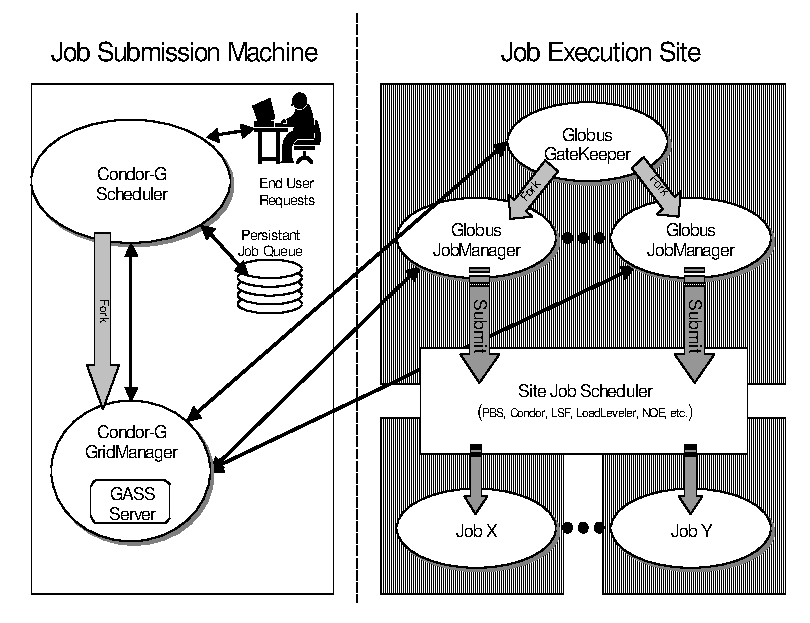
\includegraphics{grids/gfig1.eps}
\caption{\label{fig:condorg}Remote Execution by Condor-G on Globus managed resources}
\end{figure}

Figure~\ref{fig:condorg} shows how Condor-G interacts with Globus protocols.
Condor-G contains a GASS server, used to transfer the executable,
\File{stdin}, \File{stdout}, and \File{stderr} to and from
the remote job execution site.
Condor-G uses the GRAM protocol to contact the remote Globus Gatekeeper
and request that a new job manager be started.
GRAM is also used to monitor the job's progress.
Condor-G detects and intelligently handles cases
such as if the remote Globus resource crashes.

%%%%%%%%%%%%%%%%%%%%%%%%%%%%%%%%%%%%%%%%%%%%%%%%%%%%%%%%%%%%%%%%%%%%%%%%%%%
\subsection{\label{sec:Condor-G-Setup}Set Up of Condor-G}
%%%%%%%%%%%%%%%%%%%%%%%%%%%%%%%%%%%%%%%%%%%%%%%%%%%%%%%%%%%%%%%%%%%%%%%%%%%

%%%%%%%%%%%%%%%%%%%%%%%%%%%%%%%%%%%%%%%%%%%%%%%%%%%%%%%%%%%%%%%%%%%%%%%%%%%
\subsubsection{\label{sec:Condor-G-Install}Condor-G Installation}
%%%%%%%%%%%%%%%%%%%%%%%%%%%%%%%%%%%%%%%%%%%%%%%%%%%%%%%%%%%%%%%%%%%%%%%%%%%
\index{Condor-G!installation}
Condor-G is included in the standard Condor distribution.
Once Condor is obtained via download, installed, and configured,
(see
section~\ref{sec:install} on page~\pageref{sec:install})
there are two steps necessary before a globus universe job
can be submitted:

\begin{enumerate}

\item{Install Globus tools.}
Three ways are listed for obtaining the Globus tools:
   \begin{enumerate}
   \item{Globus}.
   From the web page at \URL{http://www.globus.org/}, follow links to the
   globus toolkit to get the resource management client bundle.
   \item{NMI}.
   From the web page at \URL{http://www.nsf-middleware.org/}, follow links
   to the NMI Release, and then to the Components, and finally to the
   Globus Toolkit. 
   \item{VDT}.
   From the web page at \URL{http://www.griphyn.org/vdt},
   follow the link to installing and setting up the Virtual Data Toolkit.
   \end{enumerate}

\item{Configure for Condor-G.}
If you installed Condor using the submit-only option, you will
need to add the following entries to your configuration file:
\begin{verbatim}
GRIDMANAGER             = $(SBIN)/condor_gridmanager
GAHP                    = $(SBIN)/gahp_server
MAX_GRIDMANAGER_LOG     = 64000
GRIDMANAGER_DEBUG       = D_COMMAND
GRIDMANAGER_LOG         = $(LOG)/GridLogs/GridmanagerLog.$(USERNAME)
GLIDEIN_SERVER_NAME     = gridftp.cs.wisc.edu
GLIDEIN_SERVER_DIR      = /p/condor/public/binaries/glidein
\end{verbatim}

If Condor-G is installed as root, the file
set by the configuration variable
\Macro{GRIDMANAGER\_LOG} must have world-write permission.
All of the parent directories for this file must
also have world-execute permission.
The Gridmanager runs as the user who submitted the job,
so the Gridmanager may not be able to write to the ordinary 
\MacroUNI{log} directory.
%The example configuration file sets the log file to be 
%\begin{verbatim}
%GRIDMANAGER_LOG = $(LOG)/GridLogs/GridmanagerLog.$(USERNAME) 
%\end{verbatim}
Use of the definition of \MacroNI{GRIDMANAGER\_LOG}
shown above will likely require the creation of
the directory \verb@$(LOG)/GridLogs@.
Permissions on this directory should be set
by running \Prog{chmod} using the value 1777. 

Another option is to locate the Gridmanager log files
somewhere else, like so:
\begin{verbatim}
GRIDMANAGER_LOG  = /tmp/GridmanagerLog.$(USERNAME)
\end{verbatim}

If you make any changes to the configuration file while
Condor is running, you will need to issue a \Condor{reconfigure}
command.

See section~\ref{sec:Configuring-Condor} on
page~\pageref{sec:Configuring-Condor} for
more information about configuration file entries.
See section~\ref{sec:Gridmanager-Config-File-Entries} on
page~\pageref{sec:Gridmanager-Config-File-Entries} for information
about  configuration file entries specific to the Condor-G
gridmanager.

\end{enumerate}

%%%%%%%%%%%%%%%%%%%%%%%%%%%%%%%%%%%%%%%%%%%%%%%%%%%%%%%
\subsubsection{\label{sec:Condor-G-Credentials}Credential Management}
%%%%%%%%%%%%%%%%%%%%%%%%%%%%%%%%%%%%%%%%%%%%%%%%%%%%%%%

(Reword this section to talk more about credential management and less
about specific config values. Also, probably move it out of the setup
section.)

Condor-G periodically checks for an updated proxy at
an interval given by the configuration variable
\AdAttr{GRIDMANAGER\_CHECKPROXY\_INTERVAL}.
The value is defined in terms of seconds.
For example, if you create a 12-hour proxy, and then
6 hours later re-run \Prog{grid-proxy-init},
Condor-G will check the proxy within
this time interval, and use the new proxy it finds there.
The default interval is 10 minutes.

Condor-G also knows when the proxy of each job will expire,
and if the proxy is not refreshed before
\AdAttr{GRIDMANAGER\_MINIMUM\_PROXY\_TIME}
seconds before the proxy expires,
the Condor-G grid manager daemon exits.
Since the grid manager daemon keeps track of all jobs
associated with a proxy, its tasks
(such as authentication, file transfer, job log maintainance)
will not occur.
So, if
\AdAttr{GRIDMANAGER\_MINIMUM\_PROXY\_TIME}
is 180, and the proxy is 3 minutes away from
expiring, Condor-G will attempt to safely shut down,
instead of simply losing
contact with the remote job because Condor-G is unable to
authenticate the remote job.
The default setting is 3 minutes (180 seconds).

%%%%%%%%%%%%%%%%%%%%%%%%%%%%%%%%%%%%%%%%%%%%%%%%%%%%%%%%%%%%%%%%%%%%%%%%%%%
\subsection{\label{sec:Using-Condor-G}Using the Globus Universe}
%%%%%%%%%%%%%%%%%%%%%%%%%%%%%%%%%%%%%%%%%%%%%%%%%%%%%%%%%%%%%%%%%%%%%%%%%%%

\index{universe!Globus}
This section contains what users need to know to 
run and manage jobs under the globus universe.

%%%%%%%%%%%%%%%%%%%%%%%%%%%%%%%%%%%%%%%%%%%%%%%%%%%%%%%%%%%%%%%%%%%%%%%%%%%
\subsubsection{\label{sec:Running-CondorG-Job}Running a Globus Universe Job}
%%%%%%%%%%%%%%%%%%%%%%%%%%%%%%%%%%%%%%%%%%%%%%%%%%%%%%%%%%%%%%%%%%%%%%%%%%%
\index{Condor-G!job submission}

Under Condor, successful job submission to the Globus universe requires
credentials.
An X.509 certificate is used to create a proxy,
and an account, authorization, or allocation to use a grid resource
is required.
For more information on proxies and certificates,
please consult the Alliance PKI pages at 

\URL{http://archive.ncsa.uiuc.edu/SCD/Alliance/GridSecurity/}

Before submitting a job to Condor under the Globus universe,
make sure you have your Grid 
credentials and have used \Prog{grid-proxy-init} to create a proxy.

A job is submitted for execution to Condor using the
\Condor{submit} command.
\index{Condor commands!condor\_submit}
\Condor{submit} takes as an argument
the name of a file called a submit description file.
\index{submit description file!globus universe}
The following sample submit description file runs a job on
the Origin2000 at NCSA.

\begin{verbatim}
executable = test
globusscheduler = modi4.ncsa.uiuc.edu/jobmanager
universe = globus
output = test.out
log = test.log
queue
\end{verbatim} 

The 
\AdAttr{executable}
for this example is
transferred from the local machine to the remote machine.
By default, Condor transfers the executable, as well as any
files specified by the \AdAttr{input} command.
Note that this executable must be compiled for the correct
intended platform.

The \AdAttr{globusscheduler} command is dependent on the
scheduling software available on remote resource.
This required command will change based on the Grid resource
intended for execution of the job.

All Condor-G jobs (intended for execution on Globus-controlled
resources) are submitted to the globus universe.
The \verb@universe = globus@ command is required
in the submit description file.

No input file is specified for this example job.
Any output (file specified by the \AdAttr{output})
or error (file specified by the \AdAttr{error})
is transferred 
from the remote machine to the local machine as it is produced.
This implies that these files may be incomplete in the case
where the executable does not finish running on the remote resource.
The job log file is maintained on the local machine.

To submit this job to Condor-G for execution on the
remote machine, use
\begin{verbatim}
condor_submit test.submit
\end{verbatim}
where \File{test.submit} is the name of the submit description file.

Example output from 
\Condor{q} for this submission looks like:
\footnotesize
\begin{verbatim}
% condor_q


-- Submitter: wireless48.cs.wisc.edu : <128.105.48.148:33012> : wireless48.cs.wi

 ID      OWNER         SUBMITTED     RUN_TIME ST PRI SIZE CMD
   7.0   epaulson     3/26 14:08   0+00:00:00 I  0   0.0  test

1 jobs; 1 idle, 0 running, 0 held
\end{verbatim}
\normalsize

After a short time, Globus accepts the job.
Again running \Condor{q} will now result in

\footnotesize
\begin{verbatim}
% condor_q


-- Submitter: wireless48.cs.wisc.edu : <128.105.48.148:33012> : wireless48.cs.wi

 ID      OWNER         SUBMITTED     RUN_TIME ST PRI SIZE CMD
   7.0   epaulson     3/26 14:08   0+00:01:15 R  0   0.0  test

1 jobs; 0 idle, 1 running, 0 held
\end{verbatim}
\normalsize

Then, very shortly after that, the queue will be empty again,
because the job has finished:

\footnotesize
\begin{verbatim}
% condor_q


-- Submitter: wireless48.cs.wisc.edu : <128.105.48.148:33012> : wireless48.cs.wi

 ID      OWNER            SUBMITTED     RUN_TIME ST PRI SIZE CMD

0 jobs; 0 idle, 0 running, 0 held
\end{verbatim}
\normalsize


A second example of a submit description file runs the Unix \Prog{ls}
program on a different Globus resource.

\footnotesize
\begin{verbatim}
executable = /bin/ls
Transfer_Executable = false
globusscheduler = vulture.cs.wisc.edu/jobmanager
universe = globus
output = ls-test.out
log = ls-test.log
queue
\end{verbatim} 
\normalsize

In this example, the executable (the binary) has been pre-staged.
The executable is on the remote machine, and it is not to
be transferred before execution.
Note that the required 
\AdAttr{globusscheduler} and \AdAttr{universe}
commands are present.
The command
\begin{verbatim}
Transfer_Executable = FALSE
\end{verbatim}
within the submit description file identifies the executable
as being pre-staged.
In this case, the 
\AdAttr{executable}
command gives the path to the executable on the remote machine.

A third example submits a Perl script to be run as a submitted
Condor job.
The Perl script both lists and sets
environment variables for a job.
Save the following Perl script with the name \File{env-test.pl},
to be used as a Condor job executable.

\begin{verbatim}
#!/usr/bin/env perl

foreach $key (sort keys(%ENV))
{
   print "$key = $ENV{$key}\n"
}

exit 0;
\end{verbatim}

Run the Unix command
\begin{verbatim}
chmod 755 env-test.pl
\end{verbatim}
to make the Perl script executable.

Now create the following submit description file
(Replace \File{biron.cs.wisc.edu/jobmanager} with a resource
you are authorized to use.):

\footnotesize
\begin{verbatim}
executable = env-test.pl
globusscheduler = biron.cs.wisc.edu/jobmanager
universe = globus
environment = foo=bar; zot=qux
output = env-test.out
log = env-test.log
queue
\end{verbatim}
\normalsize

When the job has completed, the output file \File{env-test.out}
should contain something like this:

\footnotesize
\begin{verbatim}
GLOBUS_GRAM_JOB_CONTACT = https://biron.cs.wisc.edu:36213/30905/1020633947/
GLOBUS_GRAM_MYJOB_CONTACT = URLx-nexus://biron.cs.wisc.edu:36214
GLOBUS_LOCATION = /usr/local/globus
GLOBUS_REMOTE_IO_URL = /home/epaulson/.globus/.gass_cache/globus_gass_cache_1020633948
HOME = /home/epaulson
LANG = en_US
LOGNAME = epaulson
X509_USER_PROXY = /home/epaulson/.globus/.gass_cache/globus_gass_cache_1020633951
foo = bar
zot = qux
\end{verbatim}
\normalsize


Of particular interest is the GLOBUS\_REMOTE\_IO\_URL environment variable.
Condor-G automatically starts up a GASS remote I/O
server on the submitting machine.
Because of the potential for either side of the connection to fail,
the URL for the server cannot be passed directly to the job.
Instead, it is put into a file, and the GLOBUS\_REMOTE\_IO\_URL
environment variable points to this file. 
Remote jobs can read this file and use the URL it contains
to access the remote GASS server running inside Condor-G.
If the location
of the GASS server changes (for example, if Condor-G restarts),
Condor-G will contact the Globus gatekeeper and update this file on
the machine where the job is running.
It is therefore important that all accesses to
the remote GASS server check this file for the latest location.

The following Perl script will use the GASS server in Condor-G
to copy input files to the execute machine.
(In our case, our remote job
is just going to count the number of lines in a file.
Hopefully, your job will be a bit more productive.)

\footnotesize
\begin{verbatim}
#!/usr/bin/env perl
use FileHandle;
use Cwd;

STDOUT->autoflush();
$gassUrl = `cat $ENV{GLOBUS_REMOTE_IO_URL}`;
chomp $gassUrl;

$ENV{LD_LIBRARY_PATH} = $ENV{GLOBUS_LOCATION}. "/lib";
$urlCopy = $ENV{GLOBUS_LOCATION}."/bin/globus-url-copy";

# globus-url-copy needs a full pathname
$pwd = getcwd();
print "$urlCopy $gassUrl/etc/hosts file://$pwd/temporary.hosts\n\n";
`$urlCopy $gassUrl/etc/hosts file://$pwd/temporary.hosts`;

open(file, "temporary.hosts");
while(<file>) {
print $_;
}

exit 0;
\end{verbatim}
\normalsize

Our submit file looks like this:

\footnotesize
\begin{verbatim}
executable = gass-example.pl
globusscheduler = biron.cs.wisc.edu/jobmanager
universe = globus
output = gass.out
log = gass.log
queue
\end{verbatim}
\normalsize

There are two optional submit description file commands
of note:
\AdAttr{x509userproxy} and
\AdAttr{globusrsl}.
The \AdAttr{x509userproxy} command specifies the path to
an X.509 proxy.
The command is of the form:
\begin{verbatim}
x509userproxy = /path/to/proxy
\end{verbatim}
If this optional command is not present in the submit description file,
then Condor-G checks the value of the environment variable
\Env{X509\_USER\_PROXY} for the location of the proxy.
If this environment variable is not present, then Condor-G
looks for the proxy in the file
\File{/tmp/x509up\_u0000},
where the trailing zeros in this file name are
replaced with the Unix user id.

The \AdAttr{globusrsl} command is used to add additional
attribute settings to a job's RSL string.
The format of the \AdAttr{globusrsl} command is
\begin{verbatim}
globusrsl = (name=value)(name=value)
\end{verbatim}
An example of this command in a submit description file
\begin{verbatim}
globusrsl = (project=Test_Project)
\end{verbatim}
This example's attribute name for the additional RSL is
\verb@project@, and the value assigned is \verb@Test_Project@.

%%%%%%%%%%%%%%%%%%%%%%%%%%%%%%%%%%%%%%%%%%%%%%%%%%%%%%%%%%%%%%%%%%%%%%%%%%%
\subsubsection{\label{sec:Condor-G-Limits}Limitations of Condor-G}
%%%%%%%%%%%%%%%%%%%%%%%%%%%%%%%%%%%%%%%%%%%%%%%%%%%%%%%%%%%%%%%%%%%%%%%%%%%
% This subsubsection used to reside in the file limitations.tex.
\index{Condor-G!limitations}
Submitting jobs to run under the globus universe has not yet
been perfected.
The following is a list of known limitations:

\begin{enumerate}
\item{No checkpoints.}
\item{No matchmaking.}
\item{File transfer is limited.}
There are no file transfer mechanisms for files other
than the executable, \File{stdin}, \File{stdout}, and \File{stderr}.
\item{No job exit codes.}
Job exit codes are not available.
\item{Limited platform availability.}
Condor-G is only available on Linux, Solaris,
Digital UNIX, and IRIX.
HP-UX support will hopefully be available later.
\end{enumerate}

%%%%%%%%%%%%%%%%%%%%%%%%%%%%%%%%%%%%%%%%%%%%%%%%%%
\subsection{\label{sec:Condor-G-Matchmaking}Condor-G-Matchmaking}
%%%%%%%%%%%%%%%%%%%%%%%%%%%%%%%%%%%%%%%%%%%%%%%%%%
\index{universe!Globus}
\index{Globus}
\index{matchmaking!on the Grid}
\index{grid computing!matchmaking}

In it simplest usage, Condor-G allows users to specify the single
grid site they wish to submit their job to.
Often this is sufficient: perhaps a user knows exactly which
grid site they wish to use,
or a higher-level resource broker
(such as the European Data Grid's resource broker)
has decided which grid site should be used.
But when users have a variety of sites to choose from and there
is no other resource broker to make the decision, Condor-G can use
matchmaking to decide which grid site a job should run on. 

Please note that Condor-G's matchmaking ability is relatively
new. Work is being done to improve it and make it easier to use. For
now, please expect some rough edges. 

Condor-G uses the same matchmaking mechanism that Condor uses: the
\Condor{collector} and \Condor{negotiator} daemons, which are described in
Section~\ref{sec:Condor-Daemons}. 

Two changes are required to use Condor-G's matchmaking.
First,
advertise grid sites that are available so that they are
known and considered during the matchmaking process.
This is accomplished by writing ClassAd attributes and
using \Condor{advertise} to place the attributes into the
ClassAd used in matchmaking.
The second change is to the
submit description file.
This file needs to specify requirements that describe what
type of grid site can be used, instead of identifying a specific grid site.

% Karen had editted to this point.

%%%%%%%%%%%%%%%%%%%%%%%%%%%%%%%%%%%%%%%%%%%%%%%%%%
\subsubsection{Advertising grid sites to Condor-G}
%%%%%%%%%%%%%%%%%%%%%%%%%%%%%%%%%%%%%%%%%%%%%%%%%%

Each grid site that is available for matching purposes needs to be
advertised to the \Condor{collector}. Normally in Condor this is done
with the \Condor{startd} daemon, and you do not normally need to be
aware of the contents of this advertisement. Currently, there is no
equivalent to the \Condor{startd} daemon for advertising grid sites,
so you need have a deeper understanding. 

To properly advertise a grid site, a ClassAd need to be sent
periodically to the \Condor{collector}. A ClassAd is a list of
attributes and values that describe a job, a machine, or a grid
site. ClassAds are briefly described in
Section~\ref{sec:matchmaking-with-classads} and some of the common
attributes of machine ClassAds are described in
Section~\ref{user-man-machad}.

When you advertise a grid site, it looks very similar to a ClassAd for
a machine. In fact, the \Condor{collector} will believe it is a
machine, but with a different set of attributes. 

To advertise a grid site, you first need to describe the site in a
file. Here is a sample ClassAd that describes a grid site:

\footnotesize
\begin{verbatim}
# This is a comment
MyType                = "Machine"
TargetType            = "Job"
Name                  = "Example1_Gatekeeper"
gatekeeper_url        = "grid.example.com/jobmanager"
Requirements          = (CurMatches < 10) && (TARGET.JobUniverse == 9)
Rank                  = 0.000000
CurrentRank           = 0.000000
WantAdRevaluate       = True
UpdateSequenceNumber  = 4
CurMatches            = 0
\end{verbatim}
\normalsize

Let's look at each line:

\begin{verbatim}
# This is a comment
\end{verbatim}

Your file can have comments that begin with the hash mark (\#). 

\begin{verbatim}
MyType                = "Machine"
\end{verbatim}

Your grid site is pretending to be a single machine, for the purpose
of matchmaking. \Attr{MyType} is an attribute that the \Condor{negotiator}
daemon
will expect to be a string. Strings must be surrounded by double-quote
marks, as in this example. You may have surprising, unintuitive errors
if they are not quoted. You will always want \Attr{MyType} to be
``Machine''. 

\begin{verbatim}
TargetType            = "Job"
\end{verbatim}

This is an attribute that says the grid site (machine) wants to be
matched with a job. Leave this as it is. 


\footnotesize
\begin{verbatim}
Name                  = "Example1_Gatekeeper"
\end{verbatim}
\normalsize

You will want a unique name for each grid site. Any name is fine, as long as
it is quoted.

\footnotesize
\begin{verbatim}
gatekeeper_url        = "grid.example.com/jobmanager"
\end{verbatim}
\normalsize

This is the Globus gatekeeper contact string for your grid site. It is
probably a machine name followed by a slash followed by the name of
the jobmanager. If you have different job managers, you can only
specify one per ClassAd. 

\begin{verbatim}
UpdateSequenceNumber  = 4
\end{verbatim}

UpdateSequenceNumber is a positive number that must increase each time
you advertise a grid site. Normally you advertise your grid site
every five minutes. The \Condor{collector} daemon will discard a grid site's
ClassAd after 15 minutes if there have been no updates. A good number
to set this to is the current time in seconds (the epoch, as given by
the C \Procedure{time} function call), but if you are worried about your clock
running backward, you can set it to whatever you like. If ClassAds are
received with a sequence number older than the last ClassAd, they are
ignored. 

\begin{verbatim}
CurMatches            = 0
\end{verbatim}

This number is incremented each time a match is made for this grid
site. Unlike a normal machine ClassAd that can only be matched against
once, grid site advertisements can be matched against many time. 

You will probably want to set this number to be the number of grid
jobs that you have running on your site, and keep it updated each time
you submit a new ClassAd. If you do not specify CurMatches, Condor
will assume it is 0.

Condor will increment this number every time it makes a match against
a grid site.

\footnotesize
\begin{verbatim}
Requirements          = (CurMatches < 10) && (TARGET.JobUniverse == 9)
\end{verbatim}
\normalsize

These are the requirements that the grid site insists must be true
before it will accept a job. These could refer to features of the
job's ClassAd. In this case, we will take any globus-universe job, as
long we have less than 10 matches currently. This will ensure that
Condor-G will only run 10 jobs at your site---assuming that you keep
CurMatches up to date when jobs finish. Of course, you can edit this
statement to have different requirements. For example, if you want to
accept all jobs, you can have \ShortExpr{Requirements = True}.

\footnotesize
\begin{verbatim}
Rank                  = 0.000000
CurrentRank           = 0.000000
\end{verbatim}
\normalsize

This is a numerical ranking that will be assigned to a job. Right now
it is not used, but should be set to 0. 

\begin{verbatim}
WantAdRevaluate       = True
\end{verbatim}

The \Attr{WantAdRevaluate} attribute distinguishes grid site
ClassAds from normal machine ClassAds and allows multiple matches to
be made against a single site. It should be in your ad and should be
true. Note that True is not in quotes, and it should not be.

You can add other attributes to your ClassAd, to make it easy for a
job to decide which grid site it wants to use. For instance, if you
have pre-installed the Bamboozle software environment on your grid
site, you could advertise, \ShortExpr{HaveBamboozle = True} and
\ShortExpr{BamboozleVersion = 10}. Jobs can require a grid site that has
Bamboozle installed by extending their requirements with
\ShortExpr{HaveBamboozle == True}. (Note the double equal sign in the
requirements.) 

As an aside, we recommend that jobs that need specific applications
should bring them with them instead of relying on having them
pre-installed at a Grid site. You will have more reliable execution if
you do. 

Once you have a file that describes your site, you need to send it to
the \Condor{collector} daemon. For this, use \Condor{advertise}.
We recommend that you write a script to create the file
containing the ClassAd, then run the script every five minutes with
\Prog{cron}. The script should probably update the \Attr{CurMatches}
variable, if you
want to restrict the number of grid jobs that can be submitted at one
time. 

For \Condor{advertise}, specify \Arg{UPDATE\_STARTD\_AD} for
the update command. For example, if your ClassAd is specified in a
file named \File{grid-ad} you would do:

\footnotesize
\begin{verbatim}
    condor_advertise UPDATE_STARTD_AD grid-ad
\end{verbatim}
\normalsize

\Condor{advertise} usually uses UDP to transmit your ClassAd. In
wide-area networks, this may be insufficient. You can use TCP by
specifying the \Opt{-tcp} option. 

%%%%%%%%%%%%%%%%%%%%%%%%%%%%%%%%%%%%%%%%%%%%%%%%%%
\subsubsection{Submitting Condor-G jobs that use matchmaking}
%%%%%%%%%%%%%%%%%%%%%%%%%%%%%%%%%%%%%%%%%%%%%%%%%%

Submitting a job to Condor-G that requires matchmaking is
straightforward. Instead of specifying a particular scheduler with
globussheduler like this:

\footnotesize
\begin{verbatim}
globusscheduler = grid.example.com/jobmanager
\end{verbatim}
\normalsize

you instead specify requirements and tell Condor-G where to find the
gatekeeper URL in the grid site ClassAd:

\footnotesize
\begin{verbatim}
globusscheduler = $$(gatekeeper_url)
requirements    = TARGET.gatekeeper_url =!= UNDEFINED
\end{verbatim}
\normalsize

This will allow to run at any grid site, and will extract the
gatekeeper\_url attribute from the ClassAd. There is no magic meaning
behind gatekeeper\_url---you could use GatekeeperContactString if you
desired, as long as it is the same in both the job description and the
grid site ClassAd. 

The requirements specified here are a bit simple. Perhaps you only
want to run at a site that has the Bamboozle software installed, and
the sites that have it installed specify ``HaveBamboozle = True'', as
described above. A complete job description may look like this:

\footnotesize
\begin{verbatim}
universe        = globus
executable      = analyze_bamboozle_data
output          = aaa.$(Cluster).out
error           = aaa.$(Cluster).err
log             = aaa.log
globusscheduler = $$(gatekeeper_url)
requirements    = (HaveBamboozle == True) && (TARGET.gatekeeper_url =!= UNDEFINED)
leave_in_queue  = jobstatus == 4
queue
\end{verbatim}
\normalsize

%%%%%%%%%%%%%%%%%%%%%%%%%%%%%%%%%%%%%%%%%%%%%%%%%%
\subsubsection{Advanced usage}
%%%%%%%%%%%%%%%%%%%%%%%%%%%%%%%%%%%%%%%%%%%%%%%%%%

What if a job fails to run at a grid site due to an error? It will be
returned to the queue, and Condor will attempt to match it and
re-run it at another site. Condor isn't very clever about avoiding
sites that may be bad, but you can give it some assistance. Let's say
that you want to avoid running at the last grid site you ran at. You
could add this to your job description:

\footnotesize
\begin{verbatim}
match_list_length = 1
Rank              = TARGET.Name != LastMatchName0
\end{verbatim}
\normalsize

This will prefer to run at a grid site that was not just tried, but it
will allow the job to be run there if there is no other option. 

When you specify match\_list\_length, you provide an integer N, and
Condor will keep track of the last N matches. The oldest match will be
LastMatchName0, and next oldest will be LastMatchName1, and so on. (See
the \Condor{submit} manual page for more details.) The Rank expression
allows you to specify a numerical ranking for different matches. When
combined with match\_list\_length, you can prefer to avoid sites that
you have already run at. 

In addition, \Condor{submit} has two options to help you control
Condor-G job resubmissions and rematching.  See globus\_resubmit and
globus\_rematch in the \Condor{submit} manual page. These options are
independent of match\_list\_length.

There are some new attributes that will be added to the Job ClassAd,
and may be useful to you when you write your rank, requirements,
globus\_resubmit or globus\_rematch option. Please refer to
Section~\ref{user-man-jobad} and read about the following option:

\begin{itemize}
\item NumJobMatches
\item NumGlobusSubmits
\item NumSystemHolds
\item HoldReason
\item ReleaseReason
\item EnteredCurrentStatus
\item LastMatchTime
\item LastRejMatchTime
\item LastRejMatchReason
\end{itemize}

If you are concerned about unknown or malicious grid sites reporting
to your \Condor{collector}, you should use Condor's security options,
documented in Section~\ref{sec:Security}.

%%%%%%%%%%%%%%%%%%%%%%%%%%%%%%%%%%%%%%%%%%%%%%%%%%
\subsubsection{\label{sec:HTCondor-G-GridMonitor}The Grid Monitor}
%%%%%%%%%%%%%%%%%%%%%%%%%%%%%%%%%%%%%%%%%%%%%%%%%%
\index{Grid Monitor}
\index{grid computing!Grid Monitor}
\index{scalability!using the Grid Monitor}

HTCondor's Grid Monitor is designed to improve the scalability of
machines running the Globus Toolkit's GRAM2 gatekeeper.
Normally, this service runs a jobmanager process for 
every job submitted to the gatekeeper.
This includes both currently running jobs and jobs waiting in the queue.
Each jobmanager runs a Perl script at
frequent intervals (every 10 seconds) to poll the state of
its job in the local batch system.
For example, with 400 jobs submitted to a gatekeeper,
there will be 400 jobmanagers running,
each regularly starting a Perl script.
When a large number of jobs
have been submitted to a single gatekeeper,
this frequent polling can heavily load the gatekeeper.
When the gatekeeper is under heavy load,
the system can become non-responsive, and a variety of problems can occur.

HTCondor's Grid Monitor temporarily replaces these jobmanagers.
It is named the Grid Monitor, because it replaces the monitoring
(polling) duties previously done by jobmanagers.
When the Grid Monitor runs,
HTCondor attempts to start a single
process to poll all of a user's jobs at a given gatekeeper.
While a job is waiting in the queue, but not yet running,
HTCondor shuts down the associated jobmanager,
and instead relies on the Grid Monitor to report changes in status.
The jobmanager started to add the job to the remote
batch system queue is shut down.
The jobmanager restarts when the job begins running.

The Grid Monitor requires that the gatekeeper support the fork
jobmanager with the name \Prog{jobmanager-fork}.
If the gatekeeper does not support the fork jobmanager,
the Grid Monitor will not be used for that site.
The \Condor{gridmanager} log file reports any problems
using the Grid Monitor.

The Grid Monitor is enabled by default,
and the
configuration macro \Macro{GRID\_MONITOR} identifies
the location of the executable.


%%%%%%%%%%%%%%%%%%%%%%%%%%%%%%%%%%%%%%%%%%%%%%%%%%
\section{\label{sec:Glidein}Glidein}
%%%%%%%%%%%%%%%%%%%%%%%%%%%%%%%%%%%%%%%%%%%%%%%%%%
\index{universe!grid}
\index{HTCondor commands!condor\_glidein}
\index{glidein}
\index{grid computing!glidein}

Glidein is a mechanism by which one or more grid resources (remote machines)
temporarily join a local HTCondor pool. 
The program \Condor{glidein} is used to add a machine
to an HTCondor pool.
During the period of time when the added resource is
part of the local pool, the resource is visible 
to users of the pool.
But, by default, the resource is only available for
use by the user
that added the resource to the pool.

After glidein, the user may submit jobs for execution on the
added resource the same way that all HTCondor jobs are submitted.
To force a submitted job to run on the added resource, the
submit description file could contain a requirement that the job run 
specifically on the added resource.


%%%%%%%%%%%%%%%%%%%%%%%%%%%%%%%%%%%%%%%%%%%%%%%%%%
\subsection{What \Condor{glidein} Does}
%%%%%%%%%%%%%%%%%%%%%%%%%%%%%%%%%%%%%%%%%%%%%%%%%%

\Condor{glidein} works by installing and executing
necessary HTCondor daemons and configuration on the remote resource,
such that the resource reports to and joins the local pool.
\Condor{glidein} accomplishes two separate tasks towards
having a remote grid resource join the local HTCondor pool.
They are the set up task and the execution task.

The set up task generates necessary 
configuration files and locates proper platform-dependent
binaries for the HTCondor daemons.
A script is also generated that can be used during
the execution task to invoke the proper HTCondor daemons.
These files are copied to the remote resource as necessary.
The configuration variable \Macro{GLIDEIN\_SERVER\_URLS}
defines a list of locations from which the necessary
binaries are obtained.
Default values cause binaries to be downloaded from the 
UW site.
See 
section~\ref{param:GlideinServerURLS} 
on page~\pageref{param:GlideinServerURLS}
for a full definition of this configuration variable.

When the files are correctly in place,
the execution task starts the HTCondor daemons.
\Condor{glidein} does this by submitting an HTCondor job
to run under the grid universe.
The job runs the \Condor{master} on the remote grid resource.
The \Condor{master} invokes other daemons, which contact
the local pool's \Condor{collector} to join the pool.
The HTCondor daemons exit gracefully when no jobs run on the daemons for a
preset period of time.

Here is an example of how a glidein resource appears, similar to how
any other machine appears.  The name has a
slightly different form, in order to handle the possibility of
multiple instances of glidein daemons inhabiting a multi-processor
machine.

\footnotesize
\begin{verbatim}
% condor_status | grep denal
7591386@denal LINUX       INTEL  Unclaimed  Idle       3.700  24064  0+00:06:35

\end{verbatim}
\normalsize

%%%%%%%%%%%%%%%%%%%%%%%%%%%%%%%%%%%%%%%%%%%%%%%%%%
\subsection{Configuration Requirements in the Local Pool}
%%%%%%%%%%%%%%%%%%%%%%%%%%%%%%%%%%%%%%%%%%%%%%%%%%
\index{configuration!for glidein}
\index{glidein!configuration}

As remote grid resources join the local pool,
these resources must report to the local pool's \Condor{collector} daemon.
Security demands that the local pool's \Condor{collector} 
list all hosts from which they will accept communication.
Therefore, all remote grid resources accepted for glidein
must be given
\Macro{HOSTALLOW\_WRITE} permission.
An expected way to do this is to modify the empty variable
(within the sample configuration file)
\MacroNI{GLIDEIN\_SITES} to list all remote grid resources
accepted for glidein.
The list is a space or comma separated list of hosts.
This list is then given the proper permissions by an additional
redefinition of the \MacroNI{HOSTALLOW\_WRITE} configuration variable,
to also include the list of hosts
as in the following example.

\footnotesize
\begin{verbatim}
GLIDEIN_SITES = A.example.com, B.example.com, C.example.com
HOSTALLOW_WRITE = $(HOSTALLOW_WRITE) $(GLIDEIN_SITES)
\end{verbatim}
\normalsize
Recall that for configuration file changes to take effect,
\Condor{reconfig} must be run.

If this configuration change to the security settings on
the local HTCondor pool cannot be made,
an additional HTCondor pool that utilizes
personal HTCondor may be defined.
The single machine pool
may coexist with other instances of HTCondor.
\Condor{glidein} is executed to have the remote grid
resources join this personal HTCondor pool.

%%%%%%%%%%%%%%%%%%%%%%%%%%%%%%%%%%%%%%%%%%%%%%%%%%
\subsection{Running Jobs on the Remote Grid Resource After Glidein }
%%%%%%%%%%%%%%%%%%%%%%%%%%%%%%%%%%%%%%%%%%%%%%%%%%

Once the Globus resource has been added to the local HTCondor
pool with \Condor{glidein},
job(s) may be submitted.
To force a job to run on the Globus resource,
specify that Globus resource as a machine requirement
in the submit description file. 
Here is an example from within the submit description file
that forces submission to the Globus resource denali.mcs.anl.gov:
\begin{verbatim}
      requirements = ( machine == "denali.mcs.anl.gov" ) \
         && FileSystemDomain != "" \
         && Arch != "" && OpSys != ""
\end{verbatim}
This example requires that the job run only on denali.mcs.anl.gov,
and it prevents HTCondor from inserting the file system domain,
architecture, and operating system attributes as requirements
in the matchmaking process.
HTCondor must be told not to use the submission machine's
attributes in those cases
where the Globus resource's attributes
do not match the submission machine's attributes and your job
really is capable of running on the target machine.  You
may want to use HTCondor's file-transfer capabilities in order
to copy input and output files back and forth between the submission
and execution machine.


%%%%%%%%%%%%%%%%%%%%%%%%%%%%%%%%%%%%%%%%%%%%%%%%%%%%%%%%%%%%%%%%%%%%%%%%%%%
\subsection{\label{sec:Condor-G-Limits}Limitations of Condor-G}
%%%%%%%%%%%%%%%%%%%%%%%%%%%%%%%%%%%%%%%%%%%%%%%%%%%%%%%%%%%%%%%%%%%%%%%%%%%
\index{Condor-G!limitations}
Submitting jobs to run under the grid universe has not yet
been perfected.
The following is a list of known limitations:

\begin{enumerate}
\item{No checkpoints.}
\item{No job exit codes.}
Job exit codes are not available.
\item{Limited platform availability.}
Condor-G is only available on Linux, Solaris,
Digital UNIX, and IRIX.
HP-UX support will hopefully be available later.
\end{enumerate}

%%%%%%%%%%%%%%%%%%%%%%%%%%%%%%%%%%%%%%%%%%%%%%%%%%%%%%%%%%%%%%%%%%%%%%%%%%%%
\section{\label{sec:Condor-G-Glossary}A Condor-G Glossary}
%%%%%%%%%%%%%%%%%%%%%%%%%%%%%%%%%%%%%%%%%%%%%%%%%%%%%%%%%%%%%%%%%%%%%%%%%%%

The glossary of terms (in alphabetical order):

\begin{description} 

\item[certificate] definition of certificate.
\index{certificate!glossary definition}
\index{Condor-G!certificate}

\item[certification authority (CA)] definition of certification authority.
\index{certification authority!glossary definition}

\item[Condor-G]
\index{Condor-G!glossary definition}
A subset of the Condor system that deals with
submitting, managing, and executing jobs on grid-managed resources.

\item[GAHP] definition of GAHP
\index{GAHP!glossary definition}
\index{Condor-G!GAHP}

\item[GASS] definition of GASS (Global Access to Secondary Storage).
\index{GASS!glossary definition}
\index{Condor-G!GASS}

\item[GPT] definition of GPT (Grid Packaging Technologies).
\index{GPT!glossary definition}
\index{Condor-G!GPT}

\item[GRAM] definition of GRAM (Grid Resource Allocation and Management
protocol).
\index{GRAM!glossary definition}
\index{Condor-G!GRAM}

\item[GSI] GSI (Grid Security Infrastructure) is 
\index{GSI!glossary definition}
\index{Condor-G!GSI}
authentication and authorization software provided by Globus.
It allows a user to authenticate once,
handling further site-specific requirements.

\item[PKI] PKI (Public Key Infrastructure) is 
\index{PKI!glossary definition}
\index{Condor-G!PKI}

\item[proxy] A proxy (more formally, a proxy certificate) is
\index{proxy!glossary definition}
\index{Condor-G!proxy}
a temporary binding of a new key pair to an existing user identity.
Use of proxy certificates allow an entity to temporary delegate
their rights to remote processes or resources on the Internet. 


\item[VDT] definition of VDT.
\index{VDT!glossary definition}
\index{Condor-G!VDT}

\item[X.509] definition of X.509.
\index{X.509!glossary definition}
\index{Condor-G!X.509}

\end{description} 



\index{Condor-G|)}





% Cloud Computing
\chapter{Cloud Computing}
\label{cloud-computing}
Although HTCondor has long supported accessing cloud resources as though they
were part of the Grid, the differences between clouds and the Grid have
made it difficult to convert access into utility; a job in the Grid universe
starts a virtual machine, rather than the user's executable.

Since version 8.7.0, HTCondor has included a tool, \Condor{annex}, to help
users and administrators use cloud resources to run HTCondor jobs.

This documentation should be considered neither normative nor exhaustive:
it describes parts of \Condor{annex} as it exists and is implemented
as of v8.7.8, rather than as it ought to behave.

\input{clouds/introduction.tex}

\section{\label{sec:clouds-annex}HTCondor Annex User's Guide}

A user of \Condor{annex} may be a regular job submitter, or she may be an
HTCondor pool administrator.  This guide will cover basic \Condor{annex} usage
first, followed by advanced usage that may be of less interest to the
submitter.  Users interested in customizing \Condor{annex} should consult
section \ref{sec:clouds-services}.

\subsection{Considerations and Limitations}

When you run \Condor{annex}, you are adding (virtual) machines to an HTCondor
pool.  As a submitter, you probably don't have permission to add machines to
the HTCondor pool you're already using; generally speaking, security concerns
will forbid this.  If you're a pool administrator, you can of course add
machines to your pool as you see fit.  By default, however, \Condor{annex}
instances will only start jobs submitted by the user who started the annex,
so pool administrators using \Condor{annex} on their users' behalf will
probably want to use the \Opt{-owners} option or \Opt{-no-owner} flag;
see the man page (section \ref{man-condor-annex}).  Once the new machines
join the pool, they will run jobs as normal.

Submitters, however, will have to set up their own personal HTCondor pool,
so that \Condor{annex} has a pool to join, and then work with their pool
administrator if they want to move their existing jobs to their new pool.
Otherwise, jobs will have to be manually divided (removed from one and
resubmitted to the other) between the pools.  For instructions on creating
a personal HTCondor pool, preparing an AWS account for use by \Condor{annex},
and then configuring \Condor{annex} to use that account, see
section~\ref{sec:clouds-annex-first-time}.

Starting in v8.7.1, \Condor{annex} will check for inbound access to the
collector (usually port 9618) before starting an annex (it does not
support other network topologies).  When checking connectivity
from AWS, the IP(s) used by the AWS Lambda function implementing this check
may not be in the same range(s) as those used by AWS instance; please
consult AWS's list of all their IP
ranges\footnote{\URL{https://ip-ranges.amazonaws.com/ip-ranges.json}}
when configuring your firewall.

Starting in v8.7.2, \Condor{annex} requires that the AWS secret (private) key file
be owned by the submitting user and not readable by anyone else.  This
helps to ensure proper attribution.

\subsection{Basic Usage}

%% A quick-start guide with basic usage information is kept on our Wiki:
%%
%% This Wiki page should be frozen and migrated into the manual for
%% the stable release (v8.8.0); ideally, this would also be a reasonable
%% thing to do for the next development series (v8.9) as well.
%%
%% \URL{https://htcondor-wiki.cs.wisc.edu/index.cgi/wiki?p=HowToUseCondorAnnexWithOnDemandInstancesEightSevenFour}.

This section assumes you're logged into a Linux machine an that you've
already configured \Condor{annex}.  If you haven't, see
section~\ref{sec:clouds-annex-first-time}.

All the terminal commands (shown in a box without a title) and file edits
(shown in a box with an \emph{emphasized filename} for a title) in this
section take place on the Linux machine.  In this section, we follow the
common convention that the commands you type are preceded by by `\$'
to distinguish them from any expected output; don't copy that part of each
of the following lines.  (Lines which end in a `\textbackslash' continue on
the following line; be sure to copy both lines.  Don't copy the
`\textbackslash' itself.)

\subsubsection{What You'll Need to Know}

To create a HTCondor annex with on-demand instances, you'll need to know two
things:

\begin{enumerate}
\item A name for it.  ``MyFirstAnnex'' is a fine name for your first annex.
\item How many instances you want.  For your first annex, when you're checking to make sure things work, you may only want one instance.
\end{enumerate}

\subsection{Start an Annex}

Entering the following command will start an annex named ``MyFirstAnnex'' with
one instance.  \Condor{annex} will print out what it's going to do, and then
ask you if that's OK.  You must type `yes' (and hit enter) at the prompt to
start an annex; if you do not, \Condor{annex} will print out instructions
about how to change whatever you may not like about what it said it was going
to do, and then exit.

\terminal{%
\$ condor\_annex -count 1 -annex-name MyFirstAnnex \\
Will request 1 m4.large on-demand instance for 0.83 hours.  Each instance will \\
terminate after being idle for 0.25 hours. \\
Is that OK?  (Type 'yes' or 'no'): yes \\
Starting annex... \\
Annex started.  Its identity with the cloud provider is \\
'TestAnnex0\_f2923fd1-3cad-47f3-8e19-fff9988ddacf'.  It will take about three \\
minutes for the new machines to join the pool.
}

You won't need to know the annex's identity with the cloud provider unless
something goes wrong.

Before starting the annex, \Condor{annex} (v8.7.1 and later) will check to make sure that the
instances will be able to contact your pool.  Contact the Linux machine's
administrator if \Condor{annex} reports a problem with this step.

\subsubsection{Instance Types}

Each instance type provides a different number (and/or type) of CPU cores,
amount of RAM, local storage, and the like.  We recommend starting with
`m4.large', which has 2 CPU cores and 8 GiB of RAM, but you can see the
complete list of instance types at the following URL:\\
\\
\url{https://aws.amazon.com/ec2/instance-types/}\\
\\
You can specify an instance type with
the \texttt{-aws-on-demand-instance-type} flag.

\subsubsection{Leases}

By default, \Condor{annex} arranges for your annex's instances to be terminated
after \texttt{0.83} hours (50 minutes) have passed.  Once it's in place, this
lease doesn't depend on the Linux machine, but it's only checked every five
minutes, so give your deadlines a lot of cushion to make you don't get charged
for an extra hour.  The lease is intended to help you conserve money by
preventing the annex instances from accidentally running forever.
You can specify a lease duration (in decimal hours)
with the \texttt{-duration} flag.

\begin{samepage}
If you need to adjust the lease for a particular annex, you may do so by
specifying an annex name and a duration, but not a count.  When you do so,
the new duration is set starting at the current time.  For example, if you'd
like ``MyFirstAnnex'' to expire eight hours from now:

\terminal{%
\$ condor\_annex -annex-name MyFirstAnnex -duration 8 \\
Lease updated.
}
\end{samepage}

\subsubsection{Idle Time}

By default, \Condor{annex} will configure your annex's instances to terminate
themselves after being idle for \texttt{0.25} hours (fifteen minutes).  This
is intended to help you conserve money in case of problems or an extended
shortage of work.  As noted in the example output above, you can specify a max
idle time (in decimal hours) with the \texttt{-idle} flag.  \Condor{annex}
considers an instance idle if it's unclaimed (see
section~\ref{state:unclaimed} for a definition), so it won't get tricked by
jobs with long quiescent periods.

\subsubsection{Multiple Annexes}

You may have up to fifty (or fewer, depending what else you're doing with your
AWS account) differently-named annexes running at the same time.  Running
\Condor{annex} again with the same annex name before stopping that annex will
both add instances to it and change its duration.  Only instances which start
up after an invocation of \Condor{annex} will respect that invocation's max
idle time.  That may include instances still starting up from your previous
(first) invocation of \Condor{annex}, so be sure your instances have all
joined the pool before running \Condor{annex} again with the same annex name
if you're changing the max idle time.  Each invocation of \Condor{annex}
requests a certain number of instances of a given type; you may specify
the instance type, the count, or both with each invocation, but doing so
does not change the instance type or count of any previous request.

\subsection{Monitor your Annex}

\begin{samepage}
You can find out if an instance has successfully joined the pool in the
following way:

{\obeyspaces\terminal{%
\$ condor\_annex status \\
Name                               OpSys      Arch   State     Activity     Load \\
\\
slot1@ip-172-31-48-84.ec2.internal LINUX      X86\_64 Unclaimed Benchmarking  0.0 \\
slot2@ip-172-31-48-84.ec2.internal LINUX      X86\_64 Unclaimed Idle          0.0 \\
\\
\hphantom{xxxxxxxxxxxxxxx}Total Owner Claimed Unclaimed Matched Preempting Backfill  Drain \\
\\
\hphantom{xx}X86\_64/LINUX     2     0       0         2       0          0        0      0 \\
\hphantom{xxxxxxxxx}Total     2     0       0         2       0          0        0      0
}}
\end{samepage}

This example shows that the annex instance you requested has joined your pool.
(The default annex image configures one static slot for each CPU it finds on
start-up.)

\begin{samepage}
You may instead use \Condor{status}:

{\obeyspaces\terminal{%
\$ condor\_status -annex MyFirstAnnex \\
slot1@ip-172-31-48-84.ec2.internal  LINUX     X86\_64 Unclaimed Idle 0.640 3767 \\
slot2@ip-172-31-48-84.ec2.internal  LINUX     X86\_64 Unclaimed Idle 0.640 3767 \\
\\
\hphantom{xxxxxxxxxxxxxx} Total Owner Claimed Unclaimed Matched Preempting Backfill  Drain \\
\hphantom{xx}X86\_64/LINUX     2     0       0         2       0          0        0      0 \\
\hphantom{xxxxxxxxx}Total     2     0       0         2       0          0        0      0
}}
\end{samepage}

\begin{samepage}
You can also get a report about the instances which have not joined your pool:

{\obeyspaces\terminal{%
\$ condor\_annex -annex MyFirstAnnex -status \\
STATE          COUNT \\
pending            1 \\
TOTAL              1
\\
Instances not in the pool, grouped by state: \\
pending i-06928b26786dc7e6e
}}
\end{samepage}

\subsubsection{Multiple Annexes}

The following command reports on all annex instance which have joined the pool,
regardless of which annex they're from:

{\obeyspaces\terminal{%
\$ condor\_status -annex \\
slot1@ip-172-31-48-84.ec2.internal  LINUX     X86\_64 Unclaimed Idle 0.640 3767 \\
slot2@ip-172-31-48-84.ec2.internal  LINUX     X86\_64 Unclaimed Idle 0.640 3767 \\
slot1@ip-111-48-85-13.ec2.internal  LINUX     X86\_64 Unclaimed Idle 0.640 3767 \\
slot2@ip-111-48-85-13.ec2.internal  LINUX     X86\_64 Unclaimed Idle 0.640 3767 \\
\\
\hphantom{xxxxxxxxxxxxxxx}Total Owner Claimed Unclaimed Matched Preempting Backfill  Drain \\
\hphantom{xx}X86\_64/LINUX     4     0       0         4       0          0        0      0 \\
\hphantom{xxxxxxxxx}Total     4     0       0         4       0          0        0      0
}}

\begin{samepage}
The following command reports about instance which have not joined the pool,
regardless of which annex they're from:

{\obeyspaces\terminal{%
\$ condor\_annex -status \\
NAME                        TOTAL running \\
NamelessTestA                   2       2 \\
NamelessTestB                   3       3 \\
NamelessTestC                   1       1 \\
\\
NAME                        STATUS  INSTANCES... \\
NamelessTestA               running i-075af9ccb40efb162 i-0bc5e90066ed62dd8 \\
NamelessTestB               running i-02e69e85197f249c2 i-0385f59f482ae6a2e \\ i-06191feb755963edd \\
NamelessTestC               running i-09da89d40cde1f212
}}
\end{samepage}

The ellipsis in the last column (\texttt{INSTANCES...}) is to indicate that
it's a very wide column and may wrap (as it has in the example),
not that it has been truncated.

The following command combines these two reports:

{\obeyspaces\terminal{%
\$ condor\_annex status \\
Name                               OpSys      Arch   State     Activity     Load \\
\\
slot1@ip-172-31-48-84.ec2.internal LINUX      X86\_64 Unclaimed Benchmarking  0.0 \\
slot2@ip-172-31-48-84.ec2.internal LINUX      X86\_64 Unclaimed Idle          0.0 \\
\\
\hphantom{xxxxxxxxxxxxxxx}Total Owner Claimed Unclaimed Matched Preempting Backfill  Drain \\
\\
\hphantom{xx}X86\_64/LINUX     2     0       0         2       0          0        0      0 \\
\hphantom{xxxxxxxxx}Total     2     0       0         2       0          0        0      0 \\
\\
Instance ID         not in Annex  Status  Reason (if known) \\
i-075af9ccb40efb162 NamelessTestA running - \\
i-0bc5e90066ed62dd8 NamelessTestA running - \\
i-02e69e85197f249c2 NamelessTestB running - \\
i-0385f59f482ae6a2e NamelessTestB running - \\
i-06191feb755963edd NamelessTestB running - \\
i-09da89d40cde1f212 NamelessTestC running -
}}

\subsection{Run a Job}

Starting in v8.7.1, the default behaviour for an annex instance is to run only
jobs submitted by the user who ran the \Condor{annex} command.  If you'd
like to allow other users to run jobs, list them (separated by commas; don't forget
to include yourself) as arguments to the \texttt{-owner} flag when you start
the instance.  If you're creating an annex for general use, use the
\texttt{-no-owner} flag to run jobs from anyone.

Also starting in v8.7.1, the default behaviour for an annex instance is to run
only jobs which have the \texttt{MayUseAWS} attribute set (to true).  To
submit a job with \texttt{MayUseAWS} set to true, add
\texttt{+MayUseAWS = TRUE} to the submit file somewhere before the
\texttt{queue} command.  To allow an existing job to run in the annex,
use \texttt{condor\_q\_edit}.  For instance, if you'd like cluster 1234 to run
on AWS:

\terminal{%
\$ condor\_qedit 1234 "MayUseAWS = TRUE" \\
Set attribute "MayUseAWS" for 21 matching jobs.
}

\subsection{Stop an Annex}

The following command shuts HTCondor off on each instance in the annex; if
you're using the default annex image, doing so causes each instance to shut
itself down.  HTCondor does \emph{not} provide a direct method terminating
\Condor{annex} instances.

\terminal{%
\$ condor\_off -annex MyFirstAnnex \\
Sent "Kill-Daemon" command for "master" to master ip-172-31-48-84.ec2.internal
}

\subsubsection{Multiple Annexes}

The following command turns off all annex instances in your pool, regardless
of which annex they're from:

\terminal{%
\$ condor\_off -annex \\
Sent "Kill-Daemon" command for "master" to master ip-172-31-48-84.ec2.internal \\
Sent "Kill-Daemon" command for "master" to master ip-111-48-85-13.ec2.internal
}

\subsection{Using Different or Multiple AWS Regions}

It sometimes advantageous to use multiple AWS regions, or convenient to use
an AWS region other than the default, which is \Expr{us-east-1}).  To change
the default, set the configuration macro \Macro{ANNEX\_DEFAULT\_AWS\_REGION}
to the new default.  (If you used the \Condor{annex} automatic setup, you
can edit the \Expr{user\_config} file in \Expr{.condor} directory in
your home directory.)  Once you do this, you'll have to re-do the setup,
as setup is region-specific.

If you'd like to use multiple AWS regions, you can specify which reason to use
on the command line with the \Opt{-aws-region} flag.  Each region may have
zero or more annexes active simultaneously.

\subsection{Advanced Usage}

The previous section covered using what AWS calls ``on-demand''
instances.  (An ``instance'' is ``a single occurrence of something,'' in
this case, a virtual machine.  The intent is to distinguish between the
active process that's pretending to be a real piece of hardware --
the ``instance'' -- and the template it used to start it up, which may also
be called a virtual machine.)  An on-demand instance has a price fixed by AWS;
once acquired, AWS will let you keep it running as long as you continue to
pay for it.

In constrast, a ``Spot'' instance has a price determined by an (automated)
auction; when you request a ``Spot'' instance, you specify the most (per hour)
you're willing to pay for that instance.  If you get an instance, however,
you pay only what the spot price is for that instance; in effect, AWS
determines the spot price by lowering it until they run out of instances
to rent.  AWS advertises savings of up to 90\% over on-demand instances.

There are two drawbacks to this cheaper type of instance: first,
you may have to wait (indefinitely) for instances to become available at
your preferred price-point; the second is that your instances may be taken
away from you before you're done with them because somebody else will pay
more for them.  (You won't be charged for the hour in which AWS kicks
you off an instance, but you will still owe them for all of that instance's
previous hours.)  Both drawbacks can be mitigated (but not eliminated) by
bidding the on-demand price for an instance; of course, this also minimizes
your savings.

Determining an appropriate bidding strategy is outside the purview of
this manual.

\subsubsection{Using AWS Spot Fleet}

\Condor{annex} supports Spot instances via an AWS technology called
``Spot Fleet''.  Normally, when you request instances, you request a specific
type of instance (the default on-demand instance is, for instance, `m4.large'.)
However, in many cases, you don't care too much about how many cores an
intance has -- HTCondor will automatically advertise the right number and
schedule jobs appropriately, so why would you?  In such cases -- or in
other cases where your jobs will run acceptably on more than one type of
instance -- you can make a Spot Fleet request which says something like
``give me a thousand cores as cheaply as possible'', and specify that
an `m4.large' instance has two cores, while `m4.xlarge' has four, and so
on.  (The interface actually allows you to assign arbitrary values --
like HTCondor slot weights -- to each instance
type\footnote{Strictly speaking, to each ``launch specification''; see
the explanation below, in the section \emph{AWS Instance User Data}.},
but the default value is core count.)  AWS will then divide the current price for each
instance type by its core count and request spot instances at the cheapest
per-core rate until the number of cores (not the number of instances!) has
reached a thousand, or that instance type is exhausted, at which point it will
request the next-cheapest instance type.

(At present, a Spot Fleet only chooses the cheapest price within each
AWS region; you would have to start a Spot Fleet in each AWS region you
were willing to use to make sure you got the cheapest possible price.  For
fault tolerance, each AWS region is split into independent zones, but each
zone has its own price.  Spot Fleet takes care of that detail for you.)

In order to create an annex via a Spot Fleet, you'll need a file containing
a JSON blob which describes the Spot Fleet request you'd like to make.  (It's
too complicated for a reasonable command-line interface.)  The AWS web
console can be used to create such a file; the button to download that
file is (currently) in the upper-right corner of the last page before
you submit the Spot Fleet request; it is labeled `JSON config'.  You
may need to create an IAM role the first time you make a Spot Fleet
request; please do so before running \Condor{annex}.

You \emph{must} select the instance role profile used by your on-demand
instances for \Condor{annex} to work.  This value will have been stored in the
configuration macro \Macro{ANNEX\_DEFAULT\_ODI\_INSTANCE\_PROFILE\_ARN}
by the setup procedure.

%% I should really fix it so that the ODI InstanceProfileARN is preferred
%% over the IamInstanceProfile specified in the JSON configuration file.

Specify the JSON configuration file using \Opt{-aws-spot-fleet-config-file},
or set the configuration macro \Macro{ANNEX\_DEFAULT\_SFR\_CONFIG\_FILE} to
the full path of the file you just downloaded, if you'd like it to become
your default configuration for Spot annexes.  Be aware that \Condor{annex}
does \emph{not} alter the validity period if one is set in the Spot
Fleet configuration file.  You should remove the references to `ValidFrom'
and `ValidTo' in the JSON file to avoid confusing surprises later.

Additionally, be aware that \Condor{annex} uses the Spot Fleet API in
its ``request'' mode, which means that an annex created with Spot
Fleet has the same semantics with respect to replacement as it would
otherwise: if an instance terminates for any reason, including AWS
taking it away to give to someone else, it is not replaced.

You must specify the number of cores (total instance weight; see above) using
\Opt{-slots}.  You may also specify \Opt{-aws-spot-fleet}, if you wish;
doing so may make this \Condor{annex} invocation more self-documenting.
You may use other options as normal, excepting those which begin with
\Opt{-aws-on-demand}, which indicates an option specific to on-demand
instances.

\subsubsection{Custom HTCondor Configuration}

When you specify a custom configuration, you specify the full path to a
configuration directory which will be copied to the instance.  The customizations
performed by \Condor{annex} will be applied to a temporary copy of this
directory before it is uploaded to the instance.  Those customizations
consist of creating two files: {\tt password\_file.pl} (named that way to ensure
that it isn't ever accidentally treated as configuration), and
{\tt 00ec2-dynamic.config}.  The former is a password file for use by the pool
password security method, which if configured, will be used by \Condor{annex}
automatically.  The latter is an HTCondor configuration file; it is named
so as to sort first and make it easier to over-ride with whatever configuration
you see fit.

\subsubsection{AWS Instance User Data}

HTCondor doesn't interfere with this in any way, so if you'd like to set
an instance's user data, you may do so.  However, as of v8.7.2, the
\Opt{-user-data} options don't work for on-demand instances (the default
type).  If you'd like to specify user data for your Spot Fleet -driven
annex, you may do so in four different ways: on the command-line or
from a file, and for all launch specifications or for only those launch
specifications which don't already include user data.  These two choices
correspond to the absence or presence of a trailing \Opt{-file} and the
absence or presence of \Opt{-default} immediately preceding \Opt{-user-data}.

A ``launch specification,'' in this context, means one of the virtual machine
templates you told Spot Fleet would be an acceptable way to accomodate your
resource request.  This usually corresponds one-to-one with instance types,
but this is not required.

\subsubsection{Expert Mode}

The man page (in section \ref{man-condor-annex}) lists the ``expert
mode'' options.

Four of the ``expert mode'' options set the URLs used to access AWS services,
not including the CloudFormation URL needed by the \Opt{-setup} flag.  You
may change the CloudFormation URL by changing the HTCondor configuration
macro \Macro{ANNEX\_DEFAULT\_CF\_URL}, or by supplying the URL as the third
parameter after the \Opt{-setup} flag.  If you change any of the URLs,
you may need to change all of the URLs -- Lambda functions and CloudWatch
events in one region don't work with instances in another region.

You may also temporarily specify a different AWS account by using the
access (\Opt{-aws-access-key-file}) and
secret key (\Opt{-aws-secret-key-file}) options.  Regular users may have
an accounting reason to do this.

The options labeled ``developers only'' control implementation details and
may change without warning; they are probably best left unused unless you're
a developer.

%% Developers should but don't have an option to set the connectivity-checking
%% Lambda function's name (or ARN).

\section{Using \Condor{annex} for the First Time}
\label{sec:clouds-annex-first-time}

This guide assumes that you already have an AWS account, as well as a log-in
account on a Linux machine with a public address and a system administrator
who's willing to open a port for you.  All the terminal commands (shown in a
box without a title) and file edits (shown in a box with an
\emph{emphasized title}) take place on the Linux machine.  You can perform the
web-based steps from wherever is convenient, although it will save you some
copying if you run the browser on the Linux machine.

Before using \Condor{annex} for the first time, you'll have to do three things:

\begin{enumerate}
\item install a personal HTCondor
\item prepare your AWS account
\item configure \Condor{annex}
\end{enumerate}

Instructions for each follow.

\subsection{Install a Personal HTCondor}

We recommend that you install a personal HTCondor to make use of \Condor{annex};
it's simpler to configure that way.  These instructions assume version 8.7.8
of HTCondor, but should work the 8.8.x series as well; change `8.7.8' in
the instructions wherever it appears.

These instructions assume that it's OK to create a directory named
\texttt{condor-8.7.8} in your home directory; adjust them accordingly if you
want to install HTCondor somewhere else.

Start by downloading (from
\url{https://research.cs.wisc.edu/htcondor/downloads/}) the 8.7.8 release from
the ``tarballs'' section that matches your Linux version.  (If you don't know
your Linux version, ask your system administrator.)  These instructions assume
that the file you downloaded is located in your home directory on the Linux
machine, so copy it there if necessary.

Then do the following; note that in this box, like other terminal boxes,
the commands you type are preceded by by `\$' to distinguish them from any
expected output, so don't copy that part of each of the following lines.
(Lines which end in a `\textbackslash' continue on the following line; be
sure to copy both lines.  Don't copy the `\textbackslash' itself.)

\terminal{%
\$ mkdir \textasciitilde{}/condor-8.7.8; cd \textasciitilde{}/condor-8.7.8; mkdir local \\
\$ tar -z -x -f \textasciitilde{}/condor-8.7.8-*-stripped.tar.gz \\
\$ ./condor-8.7.8-*-stripped/condor\_install --local-dir `pwd`/local \textbackslash \\
\hphantom{\$ ./}--make-personal-condor \\
\$ .\ ./condor.sh \\
\$ condor\_master
}

\subsubsection{Testing}
\label{sec:clouds-user-guide-testing}

Give HTCondor a few seconds to spin up and the try a few commands to make sure
the basics are working.  Your output will vary depending on the time of day,
the name of your Linux machine, and its core count, but it should generally be
pretty similar to the following.

% LaTeX typsets lines with a leading hyphen without the usual padding, which
% causes that line's characters not to align vertically.  We'll just elide
% the dash at the beginning of the second line so it looks right.
%
% Note that we've got the trailing % on all of these so we can have the
% first line of the [file|term]inal start in the first column of this file.
{\obeyspaces\terminal{%
\$ condor\_q \\
\hphantom{xx} Schedd: submit-3.batlab.org : <127.0.0.1:12815?... @ 02/03/17 13:57:35 \\
OWNER    BATCH\_NAME         SUBMITTED   DONE   RUN    IDLE  TOTAL JOB\_IDS \\
\\
0 jobs; 0 completed, 0 removed, 0 idle, 0 running, 0 held, 0 suspended \\
\$ condor\_status -any \\
MyType             TargetType         Name \\
\\
Negotiator         None               NEGOTIATOR \\
Collector          None               Personal Condor at 127.0.0.1@submit-3 \\
Machine            Job                slot1@submit-3.batlab.org \\
Machine            Job                slot2@submit-3.batlab.org \\
Machine            Job                slot3@submit-3.batlab.org \\
Machine            Job                slot4@submit-3.batlab.org \\
Machine            Job                slot5@submit-3.batlab.org \\
Machine            Job                slot6@submit-3.batlab.org \\
Machine            Job                slot7@submit-3.batlab.org \\
Machine            Job                slot8@submit-3.batlab.org \\
Scheduler          None               submit-3.batlab.org \\
DaemonMaster       None               submit-3.batlab.org \\
Accounting         none               <none>
}}

You should also try to submit a job; create the following file.  (We'll
refer to the contents of the box by the \emph{emphasized filename} in later
terminals and/or files.)

\fileinal{\textasciitilde{}/condor-annex/sleep.submit}{%
executable = /bin/sleep \\
arguments = 600 \\
queue
}

and submit it:

\terminal{%
\$ condor\_submit \textasciitilde{}/condor-annex/sleep.submit \\
Submitting job(s). \\
1 job(s) submitted to cluster 1. \\
\$ condor\_reschedule
}

After a little while:

{\obeyspaces\terminal{%
\$ condor\_q \\
\\
\\
\hphantom{xx} Schedd: submit-3.batlab.org : <127.0.0.1:12815?... @ 02/03/17 13:57:35 \\
OWNER    BATCH\_NAME         SUBMITTED   DONE   RUN    IDLE  TOTAL JOB\_IDS \\
tlmiller CMD: /bin/sleep   2/3  13:56      \_      1      \_      1 3.0 \\
\\
1 jobs; 0 completed, 0 removed, 0 idle, 1 running, 0 held, 0 suspended
}}

\subsubsection{Configure Public Interface}

The default personal HTCondor uses the ``loopback'' interface, which basically
just means it won't talk to anyone other than itself.  For \Condor{annex} to
work, your personal HTCondor needs to use the Linux machine's public interface.
In most cases, that's as simple as adding the following lines:

\fileinal{\textasciitilde{}/condor-8.7.8/local/condor\_config.local}{%
NETWORK\_INTERFACE = * \\
CONDOR\_HOST = \$(FULL\_HOSTNAME)
}

Restart HTCondor to force the changes to take effect:

\terminal{%
\$ condor\_restart \\
Sent "Restart" command to local master
}

To verify that this change worked, repeat the steps under section
\ref{sec:clouds-user-guide-testing}.  Then proceed onto the next section.

\subsubsection{Configure a Pool Password}

In this section, you'll configure your personal HTCondor to use a pool
password.  This is a simple but effective method of securing HTCondor's
communications to AWS.

Add the following lines:

\fileinal{\textasciitilde{}/condor-8.7.8/local/condor\_config.local}{%
SEC\_PASSWORD\_FILE = \$(LOCAL\_DIR)/condor\_pool\_password \\
SEC\_DAEMON\_INTEGRITY = REQUIRED \\
SEC\_DAEMON\_AUTHENTICATION = REQUIRED \\
SEC\_DAEMON\_AUTHENTICATION\_METHODS = PASSWORD \\
SEC\_NEGOTIATOR\_INTEGRITY = REQUIRED \\
SEC\_NEGOTIATOR\_AUTHENTICATION = REQUIRED \\
SEC\_NEGOTIATOR\_AUTHENTICATION\_METHODS = PASSWORD \\
SEC\_CLIENT\_AUTHENTICATION\_METHODS = FS, PASSWORD \\
ALLOW\_DAEMON = condor\_pool@*
}

You also need to run the following command, which prompts you to enter a
password:

\terminal{%
\$ condor\_store\_cred -c add -f `condor\_config\_val SEC\_PASSWORD\_FILE` \\
Enter password:
}

Enter a password.

\subsubsection{Tell HTCondor about the Open Port}

By default, HTCondor will use port 9618.  If the Linux machine doesn't already
have HTCondor installed, and the admin is willing to open that port, then you
don't have to do anything.  Otherwise, you'll need to add a line like the
following, replacing `9618' with whatever port the administrator opened for you.

\fileinal{\textasciitilde{}/condor-8.7.8/local/condor\_config.local}{%
COLLECTOR\_HOST = \$(FULL\_HOSTNAME):9618
}

\subsubsection{Activate the New Configuration}

Force HTCondor to read the new configuration by restarting it:

\terminal{%
\$ condor\_restart
}

\subsection{Prepare your AWS account}

Since v8.7.1, the \Condor{annex} tool has included a \texttt{-setup} command which will
prepare your AWS account.

\subsubsection{Obtaining an Access Key}

In order to use AWS, \Condor{annex} needs a pair of security tokens (like a
user name and password).  Like a user name, the ``access key'' is (more or
less) public information; the corresponding ``secret key'' is like a password
and must be kept a secret.  To help keep both halves secret,
\Condor{annex} (and HTCondor) are never told these keys directly; instead, you
tell HTCondor which file to look in to find each one.

Create those two files now; we'll tell you how to fill them in shortly.  By
convention, these files exist in your \texttt{\textasciitilde{}/.condor}
directory, which is where the \texttt{-setup} command will store the rest of
the data it needs.

\terminal{%
\$ mkdir \textasciitilde{}/.condor \\
\$ cd \textasciitilde{}/.condor \\
\$ touch publicKeyFile privateKeyFile \\
\$ chmod 600 publicKeyFile privateKeyFile
}

The last command ensures that only you can read or write to those files.

To donwload a new pair of security tokens for \Condor{annex} to use, go to
the IAM console at the following URL; log in if you need to:\\
\\
\url{https://console.aws.amazon.com/iam/home?region=us-east-1#/users}\\
\\
The following instructions assume you are logged in as a user
with the privilege to create new users.  (The `root' user for any account has
this privilege; other accounts may as well.)

\begin{enumerate}
\item Click the ``Add User'' button.
\item Enter name in the \textbf{User name} box; ``annex-user'' is a fine choice.
\item Click the check box labelled ``Programmatic access''.
\item Click the button labelled ``Next: Permissions''.
\item Select ``Attach existing policies directly''.
\item Type ``AdministratorAccess'' in the box labelled ``Filter''.
\item Click the check box on the single line that will appear below (labelled ``AdministratorAccess'').
\item Click the ``Next: review'' button (you may need to scroll down).
\item Click the ``Create user'' button.
\item From the line labelled ``annex-user'', copy the value in the column labelled ``Access key ID'' to the file \texttt{publicKeyFile}.
\item On the line labelled ``annex-user'', click the ``Show'' link in the column labelled ``Secret access key''; copy the revealed value to the file \texttt{privateKeyFile}.
\item Hit the ``Close'' button.
\end{enumerate}

The `annex-user' now has full privileges to your account.

\subsection{Configure \Condor{annex}}

The following command will setup your AWS account.  It will create a number
of persistent components, none of which will cost you anything to keep around.
These components can take quite some time to create; \Condor{annex} checks
each for completion every ten seconds and prints an additional dot (past the
first three) when it does so, to let you know that everything's still working.

\terminal{%
\$ condor\_annex -setup \\
Creating configuration bucket (this takes less than a minute)....... complete. \\
Creating Lambda functions (this takes about a minute)........ complete. \\
Creating instance profile (this takes about two minutes)................... complete. \\
Creating security group (this takes less than a minute)..... complete. \\
Setup successful.
}

\subsubsection{Checking the Setup}

You can verify at this point (or any later time) that the setup procedure
completed successfully by running the following command.

\terminal{%
\$ condor\_annex -check-setup \\
Checking for configuration bucket... OK. \\
Checking for Lambda functions... OK. \\
Checking for instance profile... OK. \\
Checking for security group... OK.
}

You're ready to run \Condor{annex}!

\subsubsection{Undoing the Setup Command}

There is not as yet a way to undo the setup command automatically, but it
won't cost you anything extra to leave your account setup for \Condor{annex}
indefinitely.  If, however, you want to be tidy, you may delete the components
setup created by going to the CloudFormation console at the following URL
and deleting the entries whose names begin with `HTCondorAnnex-':\\
\\
\url{https://console.aws.amazon.com/cloudformation/home?region=us-east-1#/stacks?filter=active}\\
\\
The setup procedure also creates an SSH key pair which may be useful
for debugging; the private key was stored in
\texttt{\textasciitilde{}/.condor/HTCondorAnnex-KeyPair.pem}.  To remove the
corresponding public key from your AWS account, go to the key pair console
at the following URL and delete the `HTCondorAnnex-KeyPair' key:\\
\\
\url{https://console.aws.amazon.com/ec2/v2/home?region=us-east-1#KeyPairs:sort=keyName}


\section{HTCondor Annex Customization Guide}\label{sec:clouds-services}

Aside from the configuration macros (see section \ref{sec:clouds-config},
below), the major way to customize \Condor{annex} is my customizing the
default disk image.  Because the implementation of \Condor{annex} varies from
service to service, and that implementation determines the constraints
on the disk image, the this section is divided by service.

\subsection{\label{sec:clouds-services-aws}Amazon Web Services}

Requirements for an Annex-compatible AMI are driven by how \Condor{annex}
securely transports HTCondor configuration and security tokens to the
instances; we will discuss that implementation briefly, to help you
understand the requirements, even though it will hopefully never matter
to you.

\subsubsection{Resource Requests}

For on-demand or Spot instances, we begin by making a single resource request
whose client token is the annex name concatenated with an underscore and then
a newly-generated GUID.  This construction allows us to terminate on-demand
instances belonging to a particular annex (by its name), as well as discover
the annex name from inside an instance.

An on-demand instance may obtain its instance ID directly from the AWS
metadata server, and then ask another AWS API for that instance ID's
client token.  Since GUIDs do not contain underscores, we can be certain
that anything to the left of the last underscore is the annex's name.

An instance started by a Spot Fleet has a client token generated by the
Spot Fleet.  Instead of performing a direct lookup, a Spot Fleet instance
must therefore determine which Spot Fleet started it, and then obtain that
Spot Fleet's client token.  A Spot Fleet will tag an instance with the
Spot Fleet's identity after the instance starts up.  This usually only
takes a few minutes, but the default image waits for up to 50 minutes,
since you're already committed to the first hour anyway.

\subsubsection{Secure Transport}

At this point, the instance knows its Annex's name.  This allows the
instance to construct the name of the tarball it should download
({\tt config-AnnexName.tar.gz}), but does not tell it from where a file
with that name should be downloaded.

(Because the user data associated with resource request is not secure,
and because we want to leave the user data available for its normal
usage, we can't just encode the tarball or its location in the user data.)

The instance determines from which S3 bucket to download by asking the
metadata server which role the instance is playing.  (An instance without
a role is unable to make use of any AWS services without acquiring valid
AWS tokens through some other method.)  The instance role created by
the setup procedure includes permission to read files matching the pattern
{\tt config-*.tar.gz} from a particular private S3 bucket.  If the instance
finds permissions matching that pattern, it assumes that the corresponding
S3 bucket is the one from which it should download, and does so; if
successful, it untars the file in {\tt /etc/condor/config.d}.

In v8.7.1, the script executing these steps is named {\tt 49ec2-instance.sh},
and is called during configuration when HTCondor first starts up.

In v8.7.2, the script executing these steps is named {\tt condor-annex-ec2},
and is called during system start-up.

The HTCondor configuration and security tokens are at this point protected
on the instance's disk by the usual filesystem permissions.  To prevent
HTCondor jobs from using the instance's permissions to do anything, but
in particular download their own copy of the security tokens, the last
thing the script does is use the Linux kernel firewall to forbid any
non-root process from accessing the metadata server.

\subsubsection{Image Requirements}

Thus, to work with \Condor{annex}, an AWS AMI must:

\begin{itemize}
\item  Fetch the HTCondor configuration and security tokens from S3;
\item  configure HTCondor to turn off after it's been idle for too long;
\item  and turn off the instance when the HTCondor master daemon exits.
\end{itemize}

The second item could be construed as optional, but if left unimplemented,
will disable the \Opt{-idle} command-line option.

The default disk image implements the above as follows:

\begin{itemize}
\item  with a configuration script ({\tt /etc/condor/49ec2-instance.sh});
\item  with a single configuration item (\Macro{STARTD\_NOCLAIM\_SHUTDOWN});
\item  with a configuration item (\Macro{DEFAULT\_MASTER\_SHUTDOWN\_SCRIPT})
and the corresponding script ({\tt /etc/condor/master\_shutdown.sh}), which
just turns around and runs {\tt shutdown -h now}.
\end{itemize}

We also strongly recommend that every \Condor{annex} disk image:

\begin{itemize}
\item  Advertise, in the master and startd, the instance ID.
\item  Use the instance's public IP, by setting \Macro{TCP\_FORWARDING\_HOST}.
\item  Turn on communications integrity and encryption.
\item  Encrypt the run directories.
\end{itemize}

The default disk image is configured to do all of this.


%%%%%%%%%%%%%%%%%%%%%%%%%%%%%%%%%%%%%%%%%%%%%%%%%%%%%%%%%%%%%%%%%%%%%%%%%%%
\subsection{\label{sec:Azure}The Azure Grid Type }
%%%%%%%%%%%%%%%%%%%%%%%%%%%%%%%%%%%%%%%%%%%%%%%%%%%%%%%%%%%%%%%%%%%%%%%%%%%
\index{Azure}
\index{Azure grid jobs}
\index{grid computing!submitting jobs to Azure}
\index{grid type!azure}

HTCondor jobs may be submitted to the Microsoft Azure
cloud service.
Azure is an on-line commercial service that provides
the rental of computers by the hour to run computational applications.
It runs virtual machine images that have been uploaded to Azure's
servers.
More information about Azure is available at
\URL{https://azure.microsoft.com}.

%%%%%%%%%%%%%%%%%%%%%%%%%%%%%%%%%%%%%%%%%%%%%%%%%%%%%%%%%%%%%%%%%%%%%%%%%%%
\subsubsection{\label{sec:Azure-submit}Azure Job Submission}
%%%%%%%%%%%%%%%%%%%%%%%%%%%%%%%%%%%%%%%%%%%%%%%%%%%%%%%%%%%%%%%%%%%%%%%%%%%

HTCondor jobs are submitted to the Azyre service
with the \SubmitCmdNI{grid} universe, setting the
\SubmitCmd{grid\_resource} command to \SubmitCmdNI{azure}, followed
by your Azure subscription id.
The submit description file command will be similar to:
\begin{verbatim}
grid_resource = azure 4843bfe3-1ebe-423e-a6ea-c777e57700a9
\end{verbatim}

Since the HTCondor job is a virtual machine image,
most of the submit description file commands
specifying input or output files are not applicable.
The \SubmitCmd{executable} command is still required,
but its value is ignored.
It identifies different jobs in the output of \Condor{q}.

The VM image for the job must already be registered a virtual
machine image in Azure.
In the submit description file,
provide the identifier for the image using
the \SubmitCmd{azure\_image} command.

This grid type requires granting HTCondor permission to use your
Azure account.
The easiest way to do this is to use the \Prog{az}
command-line tool distributed by Microsoft.
Find \Prog{az} and documentation for it at
\URL{https://docs.microsoft.com/en-us/cli/azure/?view=azure-cli-latest}.
After installation of \Prog{az},
run \Prog{az login} and follow its directions.
Once done with that step,
the tool will write authorization credentials in a file
under your HOME directory.
HTCondor will use these credentials to communicate with Azure.
% TODO better description of need for azure CLI and how to configure

You can also set up a service account in Azure for HTCondor to use.
This lets you limit the level of acccess HTCondor has to your Azure
account.
Instructions for creating a service account can be found here:
\URL{http://research.cs.wisc.edu/htcondor/gahp/AzureGAHPSetup.docx}.
% TODO Better description of creating auth file

Once you have created a file containing the service account credentials,
you can specify its location in
the submit description file using the \SubmitCmd{azure\_auth\_file} command,
as in the example:
\begin{verbatim}
azure_auth_file = /path/to/auth-file
\end{verbatim}

Azure allows the choice of different hardware configurations
for instances to run on.
Select which configuration to use for the \SubmitCmdNI{azure} grid type
with the \SubmitCmd{azure\_size} submit description file command.
HTCondor provides no default.

Azure has many locations where instances can be run (i.e. multiple
data centers distributed throughout the world).
You can select which location to use with the \SubmitCmd{azure\_location}
submit description file command.

Azure creates an administrator account within each instance, which you
can log into remote via SSH.
You can select the name of the account with the
\SubmitCmd{azure\_admin\_username} command.
You can supply the name of a file containing an SSH public key that
will allow access to the administrator account with the
\SubmitCmd{azure\_admin\_key} command.

%TODO add text about azure_image


\subsection{\label{sec:clouds-services-gcp}Google Cloud Platform}

Not implemented as of v8.7.8.



\section{\label{sec:clouds-config}HTCondor Annex Configuration}

While the configuration macros in this section may be set by the HTCondor
administrator, they are intended for the user-specific HTCondor configuration
file (usually {\tt \textasciitilde/.condor/user\_config}).  Although we
document every macro, we expect that users will generally only want to
change a few of them, listed in section \ref{sec:clouds-config-users};
the entries required in by \Condor{annex} in other sections will be
generated by its setup procedure.

Subsequent sections deal with logging
(section \ref{sec:clouds-logging}),
are for expert users
(section \ref{sec:clouds-config-experts}),
or for HTCondor developers
(section \ref{sec:clouds-config-developers}).

\subsection{\label{sec:clouds-config-users}User Settings}

\begin{description}

\label{param:AnnexDefaultLeaseDuration}
\item[\Macro{ANNEX\_DEFAULT\_LEASE\_DURATION}]
  The duration of an annex if not specified on the command-line; specified
  in seconds.  Defaults to 50 minutes.

\label{param:AnnexDefaultUnclaimedTimeout}
\item[\Macro{ANNEX\_DEFAULT\_UNCLAIMED\_TIMEOUT}]
  How long an annex instances should stay idle before shutting down;
  specified in seconds.  Defaults to 15 minutes.

\label{param:AnnexDefaultODIKeyName}
\item[\Macro{ANNEX\_DEFAULT\_ODI\_KEY\_NAME}]
  The name of the SSH key pair \Condor{annex} should use by default.
  No default.

\label{param:AnnexDefaultODIInstanceTypes}
\item[\Macro{ANNEX\_DEFAULT\_ODI\_INSTANCE\_TYPE}]
  The AWS instance type to use for on-demand instances if not specified.
  No default, but the \Condor{annex} setup procedure sets this to
  \mbox{`m4.large'}.

\label{param:AnnexDefaultODIImageID}
\item[\Macro{ANNEX\_DEFAULT\_ODI\_IMAGE\_ID}]
  The AWS AMI to use for on-demand instance if not specified.
  No default, but the \Condor{annex} setup procedure sets this to
  \mbox{`ami-35b13223'}.

\label{param:AnnexDefaultSFRConfigFile}
\item[\Macro{ANNEX\_DEFAULT\_SFR\_CONFIG\_FILE}]
  The JSON configuration file use by \Condor{annex} when creating a Spot-based
  annex.  No default.

\end{description}

\subsection{\label{sec:clouds-logging}Logging}

By default, running \Condor{annex} creates three logs: the \Condor{annex} log,
the annex GAHP log, and the annex audit log.  The default location for these
logs is the same directory as the user-specific HTCondor configuration file
(usually {\tt \textasciitilde/.condor/user\_config}).  \Condor{annex} sets the
\Macro{LOG} macro to this directory when reading its configuration.

The \Condor{annex} log is a daemon-style log.  It is configured as if
\Condor{annex} were a daemon with subsystem type \MacroNI{ANNEX};
see section \ref{sec:Daemon-Logging-Config-File-Entries} for details.

\Condor{annex} uses special helper programs, called GAHPs, to interact
with the different cloud services.  These programs do their own logging,
writing to the annex GAHP log.  The annex GAHP log is configured as if it
were a daemon, but with subsystem type \MacroNI{ANNEX\_GAHP}; see section
\ref{sec:Daemon-Logging-Config-File-Entries} for details.

The annex audit log records two lines for each invocation of \Condor{annex}:
the command as issued and the results as returned.  The location of the
audit log is set by \Macro{ANNEX\_AUDIT\_LOG}, which is the
\MacroNI{AUDIT}-level log for the \MacroNI{ANNEX} subsystem; see
\MacroNI{<SUBSYS>\_<LEVEL>\_LOG} (\ref{param:SubsysLevelLog}) for details.
Because annex creation commands typically make extensive use of values set
in configuration, \Condor{annex} will write the configuration it used for
annex creation commands into the audit log if \MacroNI{ANNEX\_DEBUG} includes
\MacroNI{D\_AUDIT:2}.

\subsection{\label{sec:clouds-config-experts}Expert Settings}

\begin{description}

\label{param:AnnexDefaultEC2URL}
\item[\Macro{ANNEX\_DEFAULT\_EC2\_URL}]
  The AWS EC2 endpoint that \Condor{annex} should use.  Defaults to
  \mbox{`https://ec2.us-east-1.amazonaws.com'}.

\label{param:AnnexDefaultCWEURL}
\item[\Macro{ANNEX\_DEFAULT\_CWE\_URL}]
  The AWS CloudWatch Events endpoint that \Condor{annex} should use.
  Defaults to \mbox{`https://events.us-east-1.amazonaws.com'}.

\label{param:AnnexDefaultLambdaURL}
\item[\Macro{ANNEX\_DEFAULT\_LAMBDA\_URL}]
  The AWS Lambda endpoint that \Condor{annex} should use.  Defaults to
  \mbox{`https://lambda.us-east-1.amazonaws.com'}.

\label{param:AnnexDefaultS3URL}
\item[\Macro{ANNEX\_DEFAULT\_S3\_URL}]
  The AWS S3 endpoint that \Condor{annex} should use.  Defaults to
  \mbox{`https://s3.amazonaws.com'}.

\label{param:AnnexDefaultCFURL}
\item[\Macro{ANNEX\_DEFAULT\_CF\_URL}]
  The AWS CloudFormation endpoint that \Condor{annex} should use.  Defaults to
  \mbox{`https://cloudformation.us-east-1.amazonaws.com'}.

\label{param:AnnexDefaultAccessKeyFile}
\item[\Macro{ANNEX\_DEFAULT\_ACCESS\_KEY\_FILE}]
  The full path to the AWS access key file \Condor{annex} should use.
  No default.

\label{param:AnnexDefaultSecretKeyFile}
\item[\Macro{ANNEX\_DEFAULT\_SECRET\_KEY\_FILE}]
  The full path to the AWS secret key file \Condor{annex} should use.
  No default.

\label{param:AnnexDefaultS3Bucket}
\item[\Macro{ANNEX\_DEFAULT\_S3\_BUCKET}]
  A private S3 bucket that the \MacroNI{ANNEX\_DEFAULT\_ACCESS\_KEY\_FILE}
  and \MacroNI{ANNEX\_DEFAULT\_SECRET\_KEY\_FILE} may write to.  No default.

\label{param:AnnexDefaultODISecurityGroupIDs}
\item[\Macro{ANNEX\_DEFAULT\_ODI\_SECURITY\_GROUP\_IDS}]
  The default security group for on-demand annexes.  Must permit inbound
  HTCondor (port 9618).

\end{description}

\subsection{\label{sec:clouds-config-developers}Developer Settings}

\begin{description}

\label{param:AnnexDefaultConnectivityFunctionARN}
\item[\Macro{ANNEX\_DEFAULT\_CONNECTIVITY\_FUNCTION\_ARN}]
  The name (or ARN) of the Lambda function on
  AWS which \Condor{annex} should use to check if the configured collector
  can be contacted from AWS.

\label{param:AnnexDefaultODIInstanceProfileARN}
\item[\Macro{ANNEX\_DEFAULT\_ODI\_INSTANCE\_PROFILE\_ARN}]
  The ARN of the instance profile \Condor{annex} should use.  No default.

\label{param:AnnexDefaultODILeaseFunctionARN}
\item[\Macro{ANNEX\_DEFAULT\_ODI\_LEASE\_FUNCTION\_ARN}]
  The Lambda function which implements the lease
  (duration) for on-demand instances.  No default.

\label{param:AnnexDefaultSFRLeaseFunctionARN}
\item[\Macro{ANNEX\_DEFAULT\_SFR\_LEASE\_FUNCTION\_ARN}]
  The Lambda function which implements the lease
  (duration) for Spot instances.  No default.

\end{description}



% APIs
\chapter{Application Programming Interfaces (APIs)}
\label{APIs}
There are several ways of interacting with the HTCondor system.  Depending on
your application and resources, the interfaces to HTCondor listed below may be
useful for your installation. If you have developed an interface to HTCondor,
please consider sharing it with the HTCondor community.

%%%%%%%%%%%%%%%%%%%%%%%%%%%%%%%%%%%%
\subsection{\label{API-WebService} Web Service}
%%%%%%%%%%%%%%%%%%%%%%%%%%%%%%%%%%%%
\index{API!Web Services}
\index{SOAP!Web Service API}
\index{Simple Object Access Protocol(SOAP)}

\Todo

%%%%%%%%%%%%%%%%%%%%%%%%%%%%%%%%%%%%
\subsection{\label{API-DRMAA} The DRMAA API}
%%%%%%%%%%%%%%%%%%%%%%%%%%%%%%%%%%%%
\index{DRMAA (Distributed Resource Management Application API)}
\index{API!DRMAA}
\index{Distributed Resource Management Application API (DRMAA)}

The following quote from the DRMAA Specification 1.0 abstract
nicely describes the purpose of the API:

The Distributed Resource Management Application API (DRMAA),
developed by a working group of the Global Grid Forum (GGF),
\begin{quote}
provides a generalized API to distributed resource management systems
(DRMSs) in order to facilitate integration of application programs.
The scope of DRMAA is limited to job submission,
job monitoring and control,
and the retrieval of the finished job status.
DRMAA provides application developers and
distributed resource management builders
with a programming model that enables
the development of distributed applications
tightly coupled to an underlying DRMS.
For deployers of such distributed applications,
DRMAA preserves flexibility and choice in system design.
\end{quote}

The API allows users who write programs using DRMAA functions
and link to a DRMAA library to submit,
control, and retrieve information about jobs to a Grid system.
The HTCondor implementation of a portion of the API
allows programs (applications) to use the library
functions provided to submit, monitor and control
HTCondor jobs.

See the DRMAA site 
(\URL{http://www.drmaa.org}) to find the
API specification for DRMA 1.0 for further details on the API.

%%%%%%%%%%%%%%%%%%%%%%%%%%%%%%%%%%%%
\subsubsection{\label{DRMAA-Implementation} Implementation Details}
%%%%%%%%%%%%%%%%%%%%%%%%%%%%%%%%%%%%


The library was developed from the DRMA API Specification 1.0 of January 2004
and the DRMAA C Bindings v0.9 of September 2003.
It is a static C library that expects a POSIX thread model
on Unix systems and a Windows thread model on Windows systems.
Unix systems that do not support POSIX threads
are not guaranteed thread safety when calling the library's functions.

The object library file is called \File{libcondordrmaa.a},
and it is located within
the \File{<release>/lib} directory in the HTCondor download.
Its header file  is called \File{lib\_condor\_drmaa.h}, and it is located within
the \File{<release>/include} directory in the HTCondor download.
Also within \File{<release>/include} is the file
\File{lib\_condor\_drmaa.README},
which gives further details on the implementation.

Use of the library requires that a
local \Condor{schedd} daemon  must be running,
and the program linked to the library must have
sufficient spool space.
This space should be in \File{/tmp}
or specified by the environment variables
\Env{TEMP}, \Env{TMP}, or \Env{SPOOL}.
The program linked to the library and the local \Condor{schedd} daemon
must have read, write, and traverse rights to the spool space.

The library currently supports the following specification-defined
job attributes:
\begin{description}
\item{DRMAA\_REMOTE\_COMMAND}
\item{DRMAA\_JS\_STATE}
\item{DRMAA\_NATIVE\_SPECIFICATION}
\item{DRMAA\_BLOCK\_EMAIL}
\item{DRMAA\_INPUT\_PATH}
\item{DRMAA\_OUTPUT\_PATH}
\item{DRMAA\_ERROR\_PATH}
\item{DRMAA\_V\_ARGV}
\item{DRMAA\_V\_ENV}
\item{DRMAA\_V\_EMAIL}
\end{description}

The attribute \Attr{DRMAA\_NATIVE\_SPECIFICATION} can be used
to direct all commands supported within
submit description files.  
See the \Condor{submit} manual page at
section~\ref{man-condor-submit} for a complete list.
Multiple commands can be specified if separated by newlines.  

As in the normal submit file,
arbitrary attributes can be added to the job's ClassAd
by prefixing the attribute with +.  In this case, you will need to put
string values in quotation marks, the same as in a submit file.

Thus to tell HTCondor that the job will likely use 64 megabytes of memory (65536
kilobytes), to more highly rank machines with more memory, and to add the
arbitrary attribute of department set to chemistry, you would set
Attr{DRMAA\_NATIVE\_SPECIFICATION} to the C string:

\begin{verbatim}
  drmaa_set_attribute(jobtemplate, DRMAA_NATIVE_SPECIFICATION,
      "image_size=65536\nrank=Memory\n+department=\"chemistry\"",
      err_buf, sizeof(err_buf)-1);

\end{verbatim}


%%%%%%%%%%%%%%%%%%%%%%%%%%%%%%%%%%%%%%%%%%%%%%%%%%%
\subsection{\label{sec:job-log-reader}The HTCondor User and Job Log Reader API}
%%%%%%%%%%%%%%%%%%%%%%%%%%%%%%%%%%%%%%%%%%%%%%%%%%%
\index{API!ReadUserLog class}
\index{User Log Reader API}
\index{Event Log Reader API}
\index{ReadUserLog class@\texttt{ReadUserLog} class}
\index{Job Log Reader API}

HTCondor has the ability to log an HTCondor job's significant events during 
its lifetime.
This is enabled in the job's submit description file with the
\SubmitCmd{Log} command.

This section describes the API defined by the C++ \Code{ReadUserLog} class,
which provides a programming interface for applications
to read and parse events,
polling for events, and saving and restoring reader state.

%%%%%%%%%%%%%%%%%%%%%%%%%%%%%%%%%%%%%%%%%%%%%%%%%%%
\subsubsection{Constants and Enumerated Types}

The following define enumerated types useful to the API.

\begin{itemize}
\item \Type{ULogEventOutcome} (defined in \File{condor\_event.h}):
  \begin{itemize}
    \item \Const{ULOG\_OK}: Event is valid
    \item \Const{ULOG\_NO\_EVENT}: No event occurred (like EOF)
    \item \Const{ULOG\_RD\_ERROR}: Error reading log file
    \item \Const{ULOG\_MISSED\_EVENT}: Missed event
    \item \Const{ULOG\_UNK\_ERROR}: Unknown Error
  \end{itemize}

\item \Type{ReadUserLog::FileStatus}
  \begin{itemize}
    \item \Const{LOG\_STATUS\_ERROR}: An error was encountered
    \item \Const{LOG\_STATUS\_NOCHANGE}: No change in file size
    \item \Const{LOG\_STATUS\_GROWN}: File has grown
    \item \Const{LOG\_STATUS\_SHRUNK}: File has shrunk
  \end{itemize}

\end{itemize}


%%%%%%%%%%%%%%%%%%%%%%%%%%%%%%%%%%%%%%%%%%%%%%%%%%%
\subsubsection{Constructors and Destructors}

All \Code{ReadUserLog} constructors invoke one of the \Code{initialize()}
methods.
Since C++ constructors cannot return errors, 
an application using any but the default constructor should call
\Code{isIinitialized()} to verify that the object initialized correctly,
and for example, had permissions to open required files.

Note that because the constructors cannot return status information,
most of these constructors will be eliminated in the future.
All constructors, except for the default constructor with no parameters,
will be removed.
The application will need to call the appropriate \Code{initialize()} method.

\begin{itemize}

\item \Constructor
  {ReadUserLog}
  {bool isEventLog}
  {default}
  \begin{itemize}
  \item \ParamDefOpt{isEventLog}{bool}{\Const{false}}
    If \Const{true}, the \Code{ReadUserLog} object is
    initialized to read the schedd-wide event log.
    \\ \Note If \Param{isEventLog} is \Const{true}, the initialization may
    silently fail, so the value of \MethodRef{ReadUserLog}{isInitialized}
    should be checked to verify that the initialization was successful.
    \\ \Note The \Param{isEventLog} parameter will be removed in the future.
  \end{itemize}

\item \Constructor
  {ReadUserLog}
  {FILE *fp, bool is\_xml, bool enable\_close}
  {of a limited functionality reader: no rotation handling, no locking}
  \begin{itemize}
  \item \ParamDef{fp}{FILE *}
    File pointer to the previously opened log file to read.
  \item \ParamDef{is\_xml}{bool}
    If \Const{true}, the file is treated as XML; otherwise, it will be
    read as an old style file.
  \item \ParamDefOpt{enable\_close}{bool}{\Const{false}}
    If \Const{true}, the reader will open the file read-only.
  \end{itemize}
  \Note The \MethodRef{ReadUserLog}{isInitialized} method
  should be invoked to verify that this constructor was initialized
  successfully.
  \\ \Note This constructor will be removed in the future.

\item \Constructor
  {ReadUserLog}
  {const char *filename, bool read\_only}
  {to read a specific log file}
  \begin{itemize}
  \item \ParamDef{filename}{const char *}
    Path to the log file to read
  \item \ParamDefOpt{read\_only}{bool}{\Const{false}}
    If \Const{true}, the reader will open the file read-only and
    disable locking.
  \end{itemize}
  \Note This constructor will be removed in the future.

\item \Constructor
  {ReadUserLog}
  {const FileState \&state, bool read\_only}
  {to continue from a persisted reader state}
  \begin{itemize}
  \item \ParamDef{state}{const FileState \&}
    Reference to the persisted state to restore from
  \item \ParamDefOpt{read\_only}{bool}{\Const{false}}
    If \Const{true}, the reader will open the file read-only and
    disable locking.
  \end{itemize}
  \Note The \MethodRef{ReadUserLog}{isInitialized}
  method should be invoked to verify that this constructor was
  initialized successfully.
  \\ \Note This constructor will be removed in the future.

\item \Destructor{ReadUserLog}

\end{itemize}


%%%%%%%%%%%%%%%%%%%%%%%%%%%%%%%%%%%%%%%%%%%%%%%%%%%
\subsubsection{Initializers}

These methods are used to perform the initialization of the
\Code{ReadUserLog} objects.  These initializers are used by all constructors
that do real work.  
Applications should never use those constructors,
should use the default constructor,
 and should instead use one of these initializer methods.

All of these functions will return \Const{false} if there are problems
such as being unable to open the log file,
or \Const{true} if successful.

\begin{itemize}

\item \MethodDef{ReadUserLog}{initialize}
  {\Type{bool}} {\Const{true}: success, \Const{false}: failed}
  {void}
  {Initialize to read the EventLog file.
  \\ \Note This method will likely be eliminated in the future, and this
  functionality will be moved to a new \Code{ReadEventLog} class.}
  \begin{itemize}\item None. \end{itemize}

\item \MethodDef{ReadUserLog}{initialize}
  {\Type{bool}} {\Const{true}: success, \Const{false}: failed}
  {const char *filename, bool handle\_rotation,
    bool check\_for\_rotated, bool read\_only}
  {Initialize to read a specific log file.}
  \begin{itemize}
  \item \ParamDef{filename}{const char *}
    Path to the log file to read
  \item \ParamDefOpt{handle\_rotation} {bool} {\Const{false}}
    If \Const{true}, enable the reader to handle rotating log files,
    which is only useful for global user logs
  \item \ParamDefOpt{check\_for\_rotated} {bool} {\Const{false}}
    If \Const{true}, try to open the rotated files
    (with file names appended with \File{.old} or \File{.1}, \File{.2}, \Dots)
    first.
  \item \ParamDefOpt{read\_only} {bool} {\Const{false}}
    If \Const{true}, the reader will open the file read-only and
    disable locking.
  \end{itemize}

\item \MethodDef{ReadUserLog}{initialize}
  {\Type{bool}} {\Const{true}: success, \Const{false}: failed}
  {const char *filename, int max\_rotation,
    bool check\_for\_rotated, bool read\_only}
  {Initialize to read a specific log file.}
  \begin{itemize}
  \item \ParamDef{filename}{const char *}
    Path to the log file to read
  \item \ParamDef{max\_rotation} {int}
    Limits what previously rotated files will be considered by the number
    given in the file name suffix.
    A value of 0 disables looking for rotated files.
    A value of 1 limits the rotated file to be that with the file name suffix
    of \File{.old}.
    As only event logs are rotated, this parameter is only useful for
    event logs.
  \item \ParamDefOpt{check\_for\_rotated} {bool} {\Const{false}}
    If \Const{true}, try to open the rotated files
    (with file names appended with \File{.old} or \File{.1}, \File{.2}, \Dots)
    first.
  \item \ParamDefOpt{read\_only} {bool} {\Const{false}}
    If \Const{true}, the reader will open the file read-only and
    disable locking.
  \end{itemize}

\item \MethodDef{ReadUserLog}{initialize}
  {\Type{bool}} {\Const{true}: success, \Const{false}: failed}
  {const FileState \&state, bool read\_only}
  {Initialize to continue from a persisted reader state.}
  \begin{itemize}
  \item \ParamDef{state}{const FileState \&}
    Reference to the persisted state to restore from
  \item \ParamDefOpt{read\_only}{bool}{\Const{false}}
    If \Const{true}, the reader will open the file read-only and
    disable locking.
  \end{itemize}

\item \MethodDef{ReadUserLog}{initialize}
  {\Type{bool}} {\Const{true}: success, \Const{false}: failed}
  {const FileState \&state, int max\_rotation, bool read\_only}
  {Initialize to continue from a persisted reader state and set the
  rotation parameters.}
  \begin{itemize}
  \item \ParamDef{state}{const FileState \&}
    Reference to the persisted state to restore from
  \item \ParamDef{max\_rotation} {int}
    Limits what previously rotated files will be considered by the number
    given in the file name suffix.
    A value of 0 disables looking for rotated files.
    A value of 1 limits the rotated file to be that with the file name suffix
    of \File{.old}.
    As only event logs are rotated, this parameter is only useful for
    event logs.
  \item \ParamDefOpt{read\_only}{bool}{\Const{false}}
    If \Const{true}, the reader will open the file read-only and
    disable locking.
  \end{itemize}

\end{itemize}

%%%%%%%%%%%%%%%%%%%%%%%%%%%%%%%%%%%%%%%%%%%%%%%%%%%
\subsubsection{Primary Methods}
\begin{itemize}

\item \MethodDef{ReadUserLog}{readEvent}
  {\Type{ULogEventOutcome}}
  {Outcome of the log read attempt. \Type{ULogEventOutcome} is an enumerated
  type.}
  {ULogEvent $*$\& event}
  {Read the next event from the log file.}
  \begin{itemize}
  \item \ParamDef{event}{\Type{ULogEvent} $*$\&}
    Pointer to an \Type{ULogEvent} that is allocated by this call to
    \MethodRef{ReadUserLog}{readEvent}.
    If no event is allocated, this pointer is
    set to \Const{NULL}.  Otherwise the event needs to be {\tt
    delete()ed} by the application.
  \end{itemize}

\item \MethodDef{ReadUserLog}{synchronize}
  {\Type{bool}} {\Const{true}: success, \Const{false}: failed}
  {void}
  {Synchronize the log file if the last event read was an error.  This
    safe guard function should be called if there is some error reading an
    event, but there are events after it in the file.
    It will skip over the
    bad event, meaning it will read up to and including the event separator,
    so that the rest of the events can be read.}
  \begin{itemize}\item None. \end{itemize}

\end{itemize}

%%%%%%%%%%%%%%%%%%%%%%%%%%%%%%%%%%%%%%%%%%%%%%%%%%%
\subsubsection{Accessors}
\begin{itemize}

\item \MethodDef{ReadUserLog}{CheckFileStatus}
  {\Type{ReadUserLog::FileStatus}}{the status of the log file, an
  enumerated type.}
  {void}
  {Check the status of the file, and whether it has grown, shrunk, etc.}
  \begin{itemize}\item None. \end{itemize}

\item \MethodDef{ReadUserLog}{CheckFileStatus}
  {\Type{ReadUserLog::FileStatus}} {the status of the log file, an
  enumerated type.}
  {bool \&is\_empty}
  {Check the status of the file, and whether it has grown, shrunk, etc.}
  \begin{itemize}
  \item \ParamDef{is\_empty}{bool \&}
    Set to \Const{true} if the file is empty, \Const{false} otherwise.
  \end{itemize}

\end{itemize}


%%%%%%%%%%%%%%%%%%%%%%%%%%%%%%%%%%%%%%%%%%%%%%%%%%%
\subsubsection{Methods for saving and restoring persistent reader state}

The \Type{ReadUserLog::FileState} structure is used to save and
restore the state of the \Type{ReadUserLog} state for persistence.  The
application should always use \Procedure{InitFileState} to initialize this
structure.

All of these methods take a reference to a state buffer
as their only parameter.

All of these methods return \Const{true} upon success.

%%%%%%%%%%%%%%%%%%%%%%%%%%%%%%%%%%%%%%%%%%%%%%%%%%%
\subsubsection{Save state to persistent storage}
To save the state, do something like this:
\footnotesize
\begin{verbatim}
  ReadUserLog                reader;
  ReadUserLog::FileState     statebuf;

  status = ReadUserLog::InitFileState( statebuf );

  status = reader.GetFileState( statebuf );
  write( fd, statebuf.buf, statebuf.size );
  ...
  status = reader.GetFileState( statebuf );
  write( fd, statebuf.buf, statebuf.size );
  ...

  status = UninitFileState( statebuf );
\end{verbatim}
\normalsize

%%%%%%%%%%%%%%%%%%%%%%%%%%%%%%%%%%%%%%%%%%%%%%%%%%%
\subsubsection{Restore state from persistent storage}
To restore the state, do something like this:
\footnotesize
\begin{verbatim}
  ReadUserLog::FileState     statebuf;
  status = ReadUserLog::InitFileState( statebuf );

  read( fd, statebuf.buf, statebuf.size );

  ReadUserLog                reader;
  status = reader.initialize( statebuf );

  status = UninitFileState( statebuf );
  ....
\end{verbatim}
\normalsize

%%%%%%%%%%%%%%%%%%%%%%%%%%%%%%%%%%%%%%%%%%%%%%%%%%%
\subsubsection{API Reference}
\begin{itemize}

\item \StaticMethodDef{ReadUserLog}{InitFileState}
  {\Type{bool}} {\Const{true} if successful, \Const{false} otherwise}
  {ReadUserLog::FileState \&state}
  {Initialize a file state buffer}
  \begin{itemize}
  \item \ParamDef{state}{ReadUserLog::FileState \&}
    The file state buffer to initialize.
  \end{itemize}

\item \StaticMethodDef{ReadUserLog}{UninitFileState}
  {\Type{bool}} {\Const{true} if successful, \Const{false} otherwise}
  {ReadUserLog::FileState \&state}
  {Clean up a file state buffer and free allocated memory}
  \begin{itemize}
  \item \ParamDef{state}{ReadUserLog::FileState \&}
    The file state buffer to un-initialize.
  \end{itemize}

\item \ConstMethodDef{ReadUserLog}{GetFileState}
  {\Type{bool}} {\Const{true} if successful, \Const{false} otherwise}
  {ReadUserLog::FileState \&state}
  {Get the current state to persist it or save it off to disk}
  \begin{itemize}
  \item \ParamDef{state}{ReadUserLog::FileState \&}
    The file state buffer to read the state into.
  \end{itemize}

\item \MethodDef{ReadUserLog}{SetFileState}
  {\Type{bool}} {\Const{true} if successful, \Const{false} otherwise}
  {const ReadUserLog::FileState \&state}
  {Use this method to set the current state, after restoring it.
    \\ \Note The state buffer is \emph{NOT} automatically updated; a call 
    \emph{MUST} be made to
    the \Procedure{GetFileState} method each time before persisting the
    buffer to disk, or however else is chosen to persist its contents.}
  \begin{itemize}
  \item \ParamDef{state}{const ReadUserLog::FileState \&}
    The file state buffer to restore from.
  \end{itemize}

\end{itemize}

%%%%%%%%%%%%%%%%%%%%%%%%%%%%%%%%%%%%%%%%%%%%%%%%%%%
\subsubsection{Access to the persistent state data}

If the application needs access to the data elements in a persistent
state, it should instantiate a \Type{ReadUserLogStateAccess} object.

\begin{itemize}
\item Constructors / Destructors

\begin{itemize}
\item \Constructor
  {ReadUserLogStateAccess}
  {const ReadUserLog::FileState \&state}
  {default}
  \begin{itemize}
  \item \ParamDef{state}{const ReadUserLog::FileState \&}
    Reference to the persistent state data to initialize from.
  \end{itemize}

\item \Destructor
  {ReadUserLogStateAccess}
\end{itemize}

\item Accessor Methods
\begin{itemize}

\item \ConstMethodDef{ReadUserLogFileState}{isInitialized}
  {\Type{bool}} {\Const{true} if successfully initialized, \Const{false} otherwise}
  {void}
  {Checks if the buffer initialized}
  \begin{itemize} \item None. \end{itemize}

\item \ConstMethodDef{ReadUserLogFileState}{isValid}
  {\Type{bool}} {\Const{true} if successful, \Const{false} otherwise}
  {void}
  {Checks if the buffer is valid for use by 
  \Procedure{ReadUserLog::initialize}}
  \begin{itemize} \item None. \end{itemize}

\item \ConstMethodDef{ReadUserLogFileState}{getFileOffset}
  {\Type{bool}} {\Const{true} if successful, \Const{false} otherwise}
  {unsigned long \&pos}
  {Get position within individual file.
    \\ \Note Can return an error if the result is too large to be
    stored in a \Type{long}.}
  \begin{itemize}
  \item \ParamDef{pos}{unsigned long \&}
    Byte position within the current log file
  \end{itemize}

\item \ConstMethodDef{ReadUserLogFileState}{getFileEventNum}
  {\Type{bool}} {\Const{true} if successful, \Const{false} otherwise}
  {unsigned long \&num}
  {Get event number in individual file.
    \\ \Note Can return an error if the result is too large to be
    stored in a \Type{long}.}
  \begin{itemize}
  \item \ParamDef{num}{unsigned long \&}
    Event number of the current event in the current log file
  \end{itemize}

\item \ConstMethodDef{ReadUserLogFileState}{getLogPosition}
  {\Type{bool}} {\Const{true} if successful, \Const{false} otherwise}
  {unsigned long \&pos}
  {Position of the start of the current file in overall log.
    \\ \Note Can return an error if the result is too large
    to be stored in a \Type{long}.}
  \begin{itemize}
  \item \ParamDef{pos}{unsigned long \&}
    Byte offset of the start of the current file in the overall
    logical log stream.
  \end{itemize}

\item \ConstMethodDef{ReadUserLogFileState}{getEventNumber}
  {bool} {\Const{true} if successful, \Const{false} otherwise}
  {unsigned long \&num}
  {Get the event number of the first event in the current file
    \\ \Note Can return an error if the result is too large
    to be stored in a \Type{long}.}
  \begin{itemize}
  \item \ParamDef{num}{unsigned long \&}
    This is the absolute event number of the first event in the
    current file in the overall logical log stream.
  \end{itemize}

\item \ConstMethodDef{ReadUserLogFileState}{getUniqId}
  {bool} {\Const{true} if successful, \Const{false} otherwise}
  {char *buf, int size}
  {Get the unique ID of the associated state file.}
  \begin{itemize}
  \item \ParamDef{buf}{char $*$}
    Buffer to fill with the unique ID of the current file.
  \item \ParamDef{size}{int}
    Size in bytes of \Param{buf}.
    \\ This is to prevent \MethodRef{ReadUserLogFileState}{getUniqId}
    from writing past the end of \Param{buf}.
  \end{itemize}

\item \ConstMethodDef{ReadUserLogFileState}{getSequenceNumber}
  {\Type{bool}} {\Const{true} if successful, \Const{false} otherwise}
  {int \&seqno}
  {Get the sequence number of the associated state file.}
  \begin{itemize}
  \item \ParamDef{seqno}{int \&}
    Sequence number of the current file
  \end{itemize}
\end{itemize}

\item Comparison Methods
\begin{itemize}

\item \ConstMethodDef{ReadUserLogFileState}{getFileOffsetDiff}
  {\Type{bool}} {\Const{true} if successful, \Const{false} otherwise}
  {const ReadUserLogStateAccess \&other, unsigned long \&pos}
  {Get the position difference of two states given by \Code{this} 
  and \Code{other}.
    \\ \Note Can return an error if the result is too large to be
    stored in a \Type{long}.}
  \begin{itemize}
  \item \ParamDef{other}{const ReadUserLogStateAccess \&}
    Reference to the state to compare to.
  \item \ParamDef{diff}{long \&}
    Difference in the positions
  \end{itemize}

\item \ConstMethodDef{ReadUserLogFileState}{getFileEventNumDiff}
  {bool} {\Const{true} if successful, \Const{false} otherwise}
  {const ReadUserLogStateAccess \&other, long \&diff}
  {Get event number in individual file.
    \\ \Note Can return an error if the result is too large to be
    stored in a \Type{long}.}
  \begin{itemize}
  \item \ParamDef{other}{const ReadUserLogStateAccess \&}
    Reference to the state to compare to.
  \item \ParamDef{diff}{long \&} Event number of the current event in
    the current log file
  \end{itemize}

\item \ConstMethodDef{ReadUserLogFileState}{getLogPosition}
  {bool} {\Const{true} if successful, \Const{false} otherwise}
  {const ReadUserLogStateAccess \&other, long \&diff}
  {Get the position difference of two states given by \Code{this} 
  and \Param{other}.
    \\ \Note Can return an error if the result is too large
    to be stored in a \Type{long}.}
  \begin{itemize}
  \item \ParamDef{other}{const ReadUserLogStateAccess \&}
    Reference to the state to compare to.
  \item \ParamDef{diff}{long \&}
    Difference between the byte offset of the start of the current
    file in the overall logical log stream and that of \Param{other}.
  \end{itemize}

\item \ConstMethodDef{ReadUserLogFileState}{getEventNumber}
  {bool} {\Const{true} if successful, \Const{false} otherwise}
  {const ReadUserLogStateAccess \&other, long \&diff}
  {Get the difference between the event number of the first event in
    two state buffers (this - other).
    \\ \Note Can return an error if the result is too large
    to be stored in a \Type{long}.}
  \begin{itemize}
  \item \ParamDef{other}{const ReadUserLogStateAccess \&}
    Reference to the state to compare to.
  \item \ParamDef{diff}{long \&}
    Difference between the absolute event number of the first event in
    the current file in the overall logical log stream and that of
    \Param{other}.
  \end{itemize}

\end{itemize}	% Comparison methods

\end{itemize}

%%%%%%%%%%%%%%%%%%%%%%%%%%%%%%%%%%%%%%%%%%%%%%%%%%%
\subsubsection{Future persistence API}
The \Type{ReadUserLog::FileState} will likely be replaced with a new
C++ \Type{ReadUserLog::NewFileState}, or a similarly named class that
will self initialize.

Additionally, the functionality of \Type{ReadUserLogStateAccess} will
be integrated into this class.

%%%%%%%%%%%%%%%%%%%%%%%%%%%%%%%%%%%%
\section{\label{API-Chirp} Chirp}
%%%%%%%%%%%%%%%%%%%%%%%%%%%%%%%%%%%%
\index{API!Chirp}
\index{Chirp API}

Chirp is a wire protocol and API that supports communication between a
running job and a chirp server.  The HTCondor system provides a Chirp
server running in the \Condor{starter} that allows a job to perform
file I/O to and from the submit machine, update attribute in its own job
ad, and append the the user log file.  This service is off by default, 
and may be enabled by setting +WantIOProxy = true in the job ad.

The Chirp protocol is fully documented at \URL{http://www3.nd.edu/~ccl/software/chirp}

To provide easier access to this wire protocol, the \Condor{chirp} 
command line tool is shipped with HTCondor.  This tool provides full
access to the chirp commands.


%%%%%%%%%%%%%%%%%%%%%%%%%%%%%%%%%%%%
\section{\label{API-commandline} The Command Line Interface}
%%%%%%%%%%%%%%%%%%%%%%%%%%%%%%%%%%%%
\index{API!Command line}
\Todo

The Condor perl module facilitates automatic submitting and monitoring of
condor jobs, along with automated administration of condor.  The most common
use of the perl module is the monitoring of condor jobs.  The condor perl
module uses the user log of a condor job for monitoring.

The Condor perl module is made up of several subroutines.  Many subroutines 
take other subroutines as arguments.  These subroutines are used as callbacks
which are called when interesting events happen.

\subsection{Subroutines}
\begin{enumerate}
	\item Submit(command\_file) \\
	The submit subroutine takes a command file name as an argument and
	submits it to condor.  The \Condor{submit} program should be in the
	path of the user.  If the user wishes to monitor the job with condor
	they must specify a log file in the command file.  The cluster
	submitted is returned. For more information
	see the \Condor{submit} man page.
	
	\item Vacate(machine) \\
	Vacate the machine specified.  The machine may be specified
	either by hostname, or by \Term{sinful string}.  For more information
	see the \Condor{vacate} man page.

	\item Reschedule(machine) \\
	Reschedule the machine specified.  The machine may be specified either
 	by hostname, or by \Term{sinful string}.  For more information see
	the \Condor{reschedule} man page.

	\item RegisterEvicted(cluster, sub) \\
	Register an eviction handler that will be called anytime a job from
	the specified cluster is evicted.  The eviction handler will be
	called with three arguments: cluster, proc, and ckpt.  The cluster
	and proc are the cluster number and process number of the job that
	was evicted.  The ckpt argument denotes whether the job was 
	checkpointed when it was evicted.

	\item RegisterNormalTerm( cluster, sub ) \\
	Register a normal termination handler that is called when a job exits
	normally.  The normal termination handler will be called with five
	arguments: cluster, proc, return\_val, output and error.  The cluster
	and proc are the cluster and process numbers of the exiting job, 
	their return\_val is the exit code of the job, and the output and error
	arguments are arrays containing the output and error produced by the
	job, one line per element.

	\item RegisterAbnormalTerm( cluster, sub ) \\
	Register an abnormal termination handler.  Works similar to 
	RegisterNormalTerm except that it is called when a job abnormally 
	exits (segmentation fault, bus error, ...) and the return\_val
	argument is replaced with two arguments: signal\_val and core.
	Signal\_val indicates the signal that the job died with and
	core indicates whether a core file was created and if so, what
	the full path to the core file is.

	\item RegisterExecute(cluster, sub) \\
	Register an execution handler that is called whenever a job starts
	running on a given host.  The handler is called with four arguments:
	cluster, proc, ip, and port.  Cluster and proc are the cluster and
	process numbers for the job, ip is the Internet address of the
	machine running the job, and port is the command port of the 
	\Condor{starter} supervising the job.

	\item RegisterSubmit(cluster, sub) \\
	Register a submit handler that is called whenever a job is submitted
	with the given cluster.  The handler is called with cluster, proc,
	ip, and port.  Cluster and proc are the cluster and
	process numbers for the job, ip is the Internet address of the
	machine running the job, and port is the command port of the 
	\Condor{schedd} responsible for the job.

	\item Monitor(cluster) \\
	Begin monitoring this cluster.  This process starts a sub process
	in order to monitor the child, so other actions may proceed in the
	main loop of the perl script.  However, handlers cannot rely on
	being able to communicate back to the main script by simply changing
	variables latter on.
	
	\item Wait() \\
	Wait until all monitors finish and exit.

	\item DebugOn() \\
	Turn debug messages on.  This may be useful if you don't understand
	what your script is doing.	
\end{enumerate}

\subsection{An Example}
The following is a simple example of using the condor perl module.
\begin{verbatim}
#!/usr/bin/perl
use Condor;

$CMD_FILE = 'mycmdfile.cmd';
$checkpoints = 0;
$evicts = 0;
$vacates = 0;

# A subroutine that will be used as the normal execution callback
$normal = sub
{
    ($cluster, $proc, $return_val, @output, @error) = @_;
    print "Job $cluster.$proc exited normally with status $return_val.\n";
    print "Job was vacated $vacates times and evicted $evicts times\n";
    print "Job checkpointed $checkpoints times\n";
    exit(0);
};	

$evicted = sub
{
    ($cluster, $proc, $ckpt) = @_;
    print "Job $cluster, $proc was evicted.\n";
    $checkpoints += $ckpt;
    $evicts++;
    &Condor::Reschedule();	
};

$execute = sub
{
    ($cluster, $proc, $ip, $port) = @_;
    print "Job running on $ip:$port, vacating...\n";
    &Condor::Vacate("\"<$ip:$port>\"");
    $vacates++;
};

$cluster = Condor::Submit($CMD_FILE);
&Condor::RegisterNormalTerm($cluster, $normal);
&Condor::RegisterEvicted($cluster, $evicted);
&Condor::RegisterExecute($cluster, $execute);
&Condor::Monitor($cluster);
&Condor::Wait();
\end{verbatim}

This example program will submit the command file 'mycmdfile.cmd' and attempt
to vacate any machine that the job runs on.  The eviction handler will
then keep track of how many times the job has checkpointed.  The termination
handler then prints out a summary of what has happened.

    



%%%%%%%%%%%%%%%%%%%%%%%%%%%%%%%%%%%%
\section{ Python Bindings}\label{API-Python}
%%%%%%%%%%%%%%%%%%%%%%%%%%%%%%%%%%%%
\index{API!Python bindings}
\index{Python bindings}

The Python module provides bindings to the client-side APIs for HTCondor and
the ClassAd language.

These Python bindings depend on loading the HTCondor shared libraries; this
means the same code is used here as the HTCondor client tools.  It is more
efficient in terms of memory and CPU to utilize these bindings than to parse
the output of the HTCondor client tools when writing applications in Python.

%%%%%%%%%%%%%%%%%%%%%%%%%%%%%%%%%%%%
\subsection{\label{Python-OtherModule} \texttt{htcondor}  Module}
%%%%%%%%%%%%%%%%%%%%%%%%%%%%%%%%%%%%
The \texttt{htcondor} module provides a client interface to the various 
HTCondor daemons. It tries to provide functionality similar to the HTCondor 
command line tools.

% 16cm is the largest width that can be handled by the pdf.
% It looks wrong in the html version.
\textbf{\texttt{htcondor} module functions:}
\begin{flushleft}
\begin{tabular}{|p{16cm}|} \hline
\texttt{platform( )}

Returns the platform of HTCondor this module is running on.
\\ \hline
\texttt{version( )}

Returns the version of HTCondor this module is linked against. 
\\ \hline
\texttt{reload\_config( )}

Reload the HTCondor configuration from disk. 
\\ \hline
\texttt{send\_command( ad, (DaemonCommands)dc, (str)target = None) }

Send a command to an HTCondor daemon specified by a location ClassAd. 

\texttt{ad} is a ClassAd specifying the location of the daemon; 
typically, found by using \texttt{Collector.locate(...)}.

\texttt{dc} is a command type; must be a member of the enum 
\texttt{DaemonCommands}. 

\texttt{target} is an optional parameter, representing an additional command
to send to a daemon.   Some commands require additional arguments; 
for example, sending \texttt{DaemonOff} to a \Condor{master} requires 
one to specify which subsystem to turn off. 
\\ \hline
\texttt{read\_events( file\_obj, is\_xml = True ) }

Read and parse an HTCondor event log file.
Returns a Python iterator of ClassAds.

Parameter \texttt{file\_obj} is a file object corresponding to an HTCondor
event log.

The optional parameter \texttt{is\_xml} specifies whether the event log is
XML-formatted.

\\ \hline

\texttt{send\_alive( ad, pid, timeout )}

Send a keep alive message to an HTCondor daemon.

Parameter \texttt{ad} is a ClassAd specifying the location of the daemon.
This ClassAd is typically found by using \texttt{Collector.locate(...)}.

Parameter \texttt{pid} is the process identifier for the keep alive.
The default value of \texttt{None} uses the value from \texttt{os.getpid()}.

Parameter \texttt{timeout} is the number of seconds that this 
keep alive is valid.
If a new keep alive is not received by the \Condor{master} in time,
then the process will be terminated.
The default value is controlled by configuration variable
\MacroNI{NOT\_RESPONDING\_TIMEOUT}.

\\ \hline

\texttt{set\_subsystem( name, type = Auto )}

Set the subsystem name for the object.

Parameter \texttt{name} is the subsystem name.

Parameter \texttt{type} is the HTCondor daemon type,
taken from the \texttt{SubsystemType} enum.
The default value of \texttt{Auto} infers the type from the
\texttt{name} parameter.

\\ \hline

\texttt{lock( file\_obj, lock\_type )}

Take a lock on a file object using the HTCondor locking protocol,
which is distinct from typical POSIX locks.
Returns a context manager object; the lock is released as
this context manager object is destroyed.

Parameter \texttt{file\_obj} is a file object corresponding to the file
which should be locked.

Parameter \texttt{lock\_type} specifies the string
\texttt{"ReadLock"} if the lock should be for reads 
or \texttt{"WriteLock"} if the lock should be for writes.

\\ \hline

\texttt{enable\_debug( )}

Enable debugging output from HTCondor, where output is sent to \texttt{stderr}.
The logging level is controlled by \MacroNI{TOOL\_DEBUG}.

\\ \hline
\texttt{enable\_log( )}

Enable debugging output from HTCondor, where output is sent to a file.
The log level is controlled by \MacroNI{TOOL\_DEBUG},
and the file used is controlled by \MacroNI{TOOL\_LOG}.

\\ \hline
\texttt{log( level, msg )}
Log a message to the HTCondor logging subsystem.

Parameter \texttt{level} is the Log category and formatting indicator.
Use the \texttt{LogLevel} enum to get list of attributes that may be
OR'd together.

Parameter \texttt{msg} is a String message to log.

\\ \hline

\texttt{poll( active\_queries )}

Wait on the results of multiple query iteratories.  Param \texttt{active\_queries}
is a list of query iterators as returned by \texttt{xquery()}.

This function returns an iterator which yields the next ready query iterator.  The
returned iterator stops when all results have been consumed for all iterators.

The iterator returned by \texttt{xquery} has a method named \texttt{nextAdsNonBlocking}
which returns a list of all ads available without blocking.

\\ \hline

\end{tabular}
\end{flushleft}

\textbf{The module object, \texttt{param}}, is
a dictionary-like object providing access to the configuration variables
in the current HTCondor configuration.

\textbf{The \texttt{Schedd} class:}
\begin{flushleft}
\begin{tabular}{|p{16cm}|} \hline

\texttt{\_\_init\_\_( classad )}

Create an instance of the \texttt{Schedd} class.  

Optional parameter \texttt{classad} 
describes the location of the remote \Condor{schedd} daemon.
If the parameter is omitted, the local \Condor{schedd} daemon is used.
\\ \hline
\texttt{transaction( flags = 0, continue\_txn = False ) }

Start a transaction with the \Condor{schedd}.
Returns a transaction context manager.
Starting a new transaction while one is ongoing is an error. 

The optional parameter \texttt{flags} defaults to 0.
Transaction flags are from the the enum \texttt{htcondor.TransactionFlags},
and the three flags are
\texttt{NonDurable}, \texttt{SetDirty}, or \texttt{ShouldLog}. 
\texttt{NonDurable} is used for performance, as it eliminates 
extra \Procedure{fsync} calls.
If the \Condor{schedd} crashes before the transaction is written to disk,
the transaction will be retried on restart of the  \Condor{schedd}. 
\texttt{SetDirty} marks the changed ClassAds as dirty,
so an update notification is sent to the \Condor{shadow} and 
the \Condor{gridmanager}. 
\texttt{ShouldLog} causes changes to the job queue to be logged
in the job event log file.

The optional parameter \texttt{continue\_txn} defaults to \texttt{false};
set the value to \texttt{true} to extend an ongoing transaction. 
\\ \hline
\texttt{act( (JobAction)action, (object)job\_spec )}

Change status of job(s) in the \Condor{schedd} daemon.
The integer return value is a \texttt{ClassAd} object describing 
the number of jobs changed.

Parameter \texttt{action} is the action to perform; must be of the
enum \texttt{JobAction}.

Parameter \texttt{job\_spec} is the job specification.
It can either be a list of job IDs or a string specifying a constraint 
to match jobs.
\\ \hline
\texttt{edit( (object)job\_spec, (str)attr, (object)value )}

Edit one or more jobs in the queue.

Parameter \texttt{job\_spec} is either a list of jobs, 
with each given as \texttt{ClusterId.ProcId} 
or a string containing a constraint to match jobs against.

Parameter \texttt{attr} is the attribute name of the attribute to edit.

Parameter \texttt{value} is the new value of the job attribute. 
It should be a string, which will be converted to a ClassAd expression,
or an \texttt{ExprTree} object.
\\ \hline
\texttt{query( constraint = true, attr\_list = [] )}

Query the \Condor{schedd} daemon for jobs.
Returns a list of ClassAds representing the matching jobs,
containing at least the requested attributes requested by the second parameter.

The optional parameter \texttt{constraint} provides a constraint for 
filtering out jobs.
It defaults to \texttt{True}.

Parameter \texttt{attr\_list} is a list of attributes for the \Condor{schedd}
daemon to project along.  
It defaults to having the \Condor{schedd} daemon return all attributes.
\\ \hline
\texttt{xquery( constraint = true, attr\_list = [], limit, opts, name )}

Query the \Condor{schedd} daemon for jobs.
Returns an iterator of ClassAds representing the matching jobs
containing at least the list of attributes requested by the second parameter.

The optional parameter \texttt{constraint} provides a constraint for
filtering out jobs.
It defaults to \texttt{True}.

Parameter \texttt{attr\_list} is a list of attributes for the \Condor{schedd}
daemon to project along.
It defaults to having the \Condor{schedd} daemon return all attributes.

Parameter \texttt{limit} is the maximum number of results this query will return.

Parameter \texttt{opts} specifies any additional query options.  Currently, the
only non-default option is \texttt{QueryOpts.AutoCluster}, which returns
autoclusters in the schedd, not jobs.

Parameter \texttt{name} provides a \textit{tag} name for the returned query iterator.
This string will always be returned from the \texttt{tag()} method of the returned
iterator.  The default value is the \Condor{schedd}'s name.  This tag is useful to identify
different queries when using the \texttt{poll()} module function.

\\ \hline

\texttt{history( (object) requirements, (list) projection, (int) match, (object) since )}

Request history records from the \Condor{schedd} daemon.
Returns an iterator to a set of ClassAds representing completed jobs.

Parameter \texttt{requirements} is either an \texttt{ExprTree} or a string 
that can be parsed as an expression.
The expression represents the requirements that all returned jobs should match. 

Parameter \texttt{projection} is a list of all the ClassAd attributes
that are to be included for each job. 
The empty list causes all attributes to be included.

Parameter \texttt{match} is an integer cap on the number of jobs to include. 

Parameter \texttt{since} is an optional argument that indicates when to stop iterating. 
It can either be an \texttt{ExprTree}, an integer or a string.
If the parameter is a string, then it is first parsed as a cluster id and then a full job id, if it does
not parse as one of these, it is assumed to be an expression and is parsed as such.  If the parameter is
an integer, then it is treated as a cluster id.
The first job that matches it will not be returned, and iteration will cease.
\\ \hline

\texttt{submit( ad, count = 1, spool = false, ad\_results = None )}

Submit one or more jobs to the \Condor{schedd} daemon.
Returns the newly created cluster ID.

This method requires the invoker to provide a ClassAd for the new job cluster;
such a ClassAd contains attributes with different names than the commands in
a submit description file.  As an example, the stdout file is referred to as
\texttt{output} in the submit description file,
but \texttt{Out} in the ClassAd.
To generate an example ClassAd, 
take a sample submit description file and invoke 

\texttt{condor\_submit -dump <filename> [cmdfile]}

Then, load the resulting contents of <filename> into Python.

Parameter \texttt{ad} is the ClassAd describing the job cluster.

Parameter \texttt{count} is the number of jobs to submit to the cluster.
Defaults to 1.

Parameter \texttt{spool} inserts the necessary attributes into the job for it
to have the input files spooled to a remote \Condor{schedd} daemon.
This parameter is necessary for jobs submitted to a remote \Condor{schedd}.

Parameter \texttt{ad\_results}, if set to a list, 
will contain the job ClassAds resulting from the job submission.
These are useful for interacting with the job spool at a later time.
\\ \hline

\texttt{submitMany( cluster\_ad, proc\_ads, spool = false, ad\_results = None )}

Submit multiple jobs to the \Condor{schedd} daemon, possibly including several
distinct processes.
Returns the newly created cluster ID.

This method requires the invoker to provide a ClassAd, \texttt{cluster\_ad} for the new job cluster;
this is the same format as in the \texttt{submit()} method.

The \texttt{proc\_ads} parameter is a list of 2-tuples; each tuple has the format
of \texttt{(proc\_ad, count)}.  For each list entry, this will result in \texttt{count} jobs being submitted
inheriting from both \texttt{cluster\_ad} and \texttt{proc\_ad}.

Parameter \texttt{spool} inserts the necessary attributes into the job for it
to have the input files spooled to a remote \Condor{schedd} daemon.
This parameter is necessary for jobs submitted to a remote \Condor{schedd}.

Parameter \texttt{ad\_results}, if set to a list,
will contain the job ClassAds resulting from the job submission.
These are useful for interacting with the job spool at a later time.

\\ \hline
\texttt{spool( ad\_list )}

Spools the files specified in a list of job ClassAds to the \Condor{schedd}.
Throws a RuntimeError exception if there are any errors.

Parameter \texttt{ad\_list} is a list of ClassAds containing job descriptions;
typically, this is the list filled by the \texttt{ad\_results} argument of the 
\texttt{submit} method call.
\\ \hline
\texttt{retrieve( job\_spec )}

Retrieve the output sandbox from one or more jobs.

Parameter \texttt{job\_spec} is an expression string matching 
the list of job output sandboxes to retrieve.
\\ \hline
\texttt{refreshGSIProxy(cluster, proc, filename, lifetime)}

Refresh the GSI proxy of a job with job identifier given
by parameters \texttt{cluster} and \texttt{proc}.
This will refresh the remote proxy with the contents of the file identified
by parameter \texttt{filename}.  

Parameter \texttt{lifetime} indicates the desired
lifetime (in seconds) of the delegated proxy.
A value of 0 specifies to not shorten the proxy lifetime.
A value of -1 specifies to use the value of configuration variable
\MacroNI{DELEGATE\_JOB\_GSI\_CREDENTIALS\_LIFETIME}.
Note that, depending on the lifetime
of the proxy in \texttt{filename}, the resulting lifetime may be shorter
than the desired lifetime.

\\ \hline
\texttt{negotiate( (str)accounting\_name )}

Begin a negotiation cycle with the remote schedd.  The \texttt{accounting\_name}
parameter determines which user we will start negotiating with.

The returned object, of type \texttt{ScheddNegotiate} is iterable; its iterator
will yield resource request ClassAds from the schedd.  Each resource request represents
a set of jobs that are next in queue for the schedd for this user.

The \texttt{ScheddNegotiate} additionally serves as a context manager, automatically
destroying the negotiation session when the context is left.

Finally, \texttt{ScheddNegotiate} has a \texttt{sendClaim} method for sending claims
back to the remote schedd based on a given resource request.

\\ \hline
\end{tabular}
\end{flushleft}

\textbf{The \texttt{Submit} class:}
\begin{flushleft}
\begin{tabular}{|p{16cm}|} \hline

\texttt{\_\_init\_\_( (dict)input = None )}

Create an instance of the \texttt{Submit} class.  

Optional parameter \texttt{input} is a Python dictionary containing
submit file key = value pairs.
If omitted, the submit class is initially empty.

\\ \hline
\texttt{expand( (str)attr )}

Expand all macros for the given attribute.

Parameter \texttt{attr} is the name of the relevant attribute.

Returns a string containing the value of the given attribute with
all macros expanded.

\\ \hline
\texttt{ queue( (object)txn, (int)count = 1, (object)ad\_results = None )}

Submit the current object to a remote queue.
Parameter \texttt{txn} is an active transaction object (see
\texttt{Schedd.transaction()}).

Optional parameter \texttt{count} is the number of procs to create
(defaults to 1 if not specified).

Optional parameter \texttt{ad\_results} is an object to receive the
ClassAd resulting from this submit.

Returns the ClusterID of the submitted job(s).

Throws a RuntimeError if the submission fails.

\\ \hline
\texttt{get( (str)attr, (str)default = None )}

Gets the value of the specified attribute.

Parameter \texttt{attr} is the name of the relevant attribute.

Optional parameter \texttt{default} is a default value to be returned
if the attribute is not defined.

Returns a string containing the value of the attribute.

\\ \hline
\texttt{setdefault( (str)attr, (str)default)}

Set a default value for an attribute.

Parameter \texttt{attr} is the name of the relevant attribute.

Parameter \texttt{default} is the value to which to set the given
attribute if that attribute has not already been set.

Returns a string containing the value of the attribute.

\\ \hline
\texttt{update( (object)submit )}

Copy the contents of a given Submit object into the current object.

Parameter \texttt{submit} is the Submit object to copy.

\\ \hline
\end{tabular}
\end{flushleft}


\textbf{The \texttt{Collector} class:}
\begin{flushleft}
\begin{tabular}{|p{16cm}|} \hline

\texttt{\_\_init\_\_( pool = None )}

Create an instance of the \texttt{Collector} class.  

Optional parameter \texttt{pool} is a string with host:port pair specified or
a list of pairs.
If omitted, the value of configuration variable \MacroNI{COLLECTOR\_HOST} 
is used.
\\ \hline
\texttt{locate( (DaemonTypes)daemon\_type, (str)name )}

Query the \Condor{collector} for a particular daemon.
Returns the ClassAd of the requested daemon.

Parameter \texttt{daemon\_type} is the type of daemon; 
must be of the enum \texttt{DaemonTypes}. 

Optional parameter \texttt{name} is the name of daemon to locate.  
If not specified, it searches for the local daemon.
\\ \hline
\texttt{locateAll( (DaemonTypes)daemon\_type )}

Query the \Condor{collector} daemon for all ClassAds of a particular type.
Returns a list of matching ClassAds.

Parameter \texttt{daemon\_type} is the type of daemon; 
must be of the enum \texttt{DaemonTypes}. 

\\ \hline
\texttt{query( (AdTypes)ad\_type, constraint=True, projection=[], (str)statistics = '' )}

Query the contents of a \Condor{collector} daemon.
Returns a list of ClassAds that match the \texttt{constraint} parameter.

Optional parameter \texttt{ad\_type} is the type of ClassAd to return,
where the types are from the enum \texttt{AdTypes}.
If not specified, the type will be \texttt{ANY\_AD}.

Optional parameter \texttt{constraint} is a constraint for the ClassAd query.
It defaults to \texttt{True}.

Optional parameter \texttt{projection} is a list of attributes.
If specified, the returned ClassAds will be projected along these attributes.

Optional parameter \texttt{statistics} is a list of statistics attributes
to include, if they exist for the specified daemon.
\\ \hline
\texttt{advertise( ad\_list, command=UPDATE\_AD\_GENERIC, use\_tcp = True )}

Advertise a list of ClassAds into the \Condor{collector}.

Parameter \texttt{ad\_list} is the list of ClassAds to advertise.

Optional parameter \texttt{command} is a command for the \Condor{collector}.
It defaults to \texttt{UPDATE\_AD\_GENERIC}.
Other commands, such as \texttt{UPDATE\_STARTD\_AD},
may require reduced authorization levels.  

Optional parameter \texttt{use\_tcp} causes updates to be sent via TCP.
Defaults to \texttt{True}.
\\ \hline
\texttt{directQuery( (Collector)arg1, (DaemonTypes)daemon\_type, (str)name = '', (list)projection = [], (str)statistics = '' )}

Query the specified daemon directly, instead of using the ClassAd from
the \Condor{collector} daemon.
Returns the ClassAd of the specified daemon, after obtaining it from the
daemon.

Parameter \texttt{arg1} is the \Condor{collector} that will identify where
to find the specified daemon.

Parameter \texttt{daemon\_type} specified a daemon with an enum from 
\texttt{DaemonTypes}.

Optional parameter \texttt{name} specifies the daemon's name.
If not specified, the local daemon is used.

Optional parameter \texttt{projection} is a list of attributes requested,
to obtain only a subset of the attributes from the ClassAd.

Optional parameter \texttt{statistics} is a list of statistics attributes
to include, if they exist for the specified daemon.
\\ \hline

\end{tabular}
\end{flushleft}

\textbf{The \texttt{Negotiator} class:}
\begin{flushleft}
\begin{tabular}{|p{16cm}|} \hline

\texttt{\_\_init\_\_( (ClassAd)ad = None ) }

Create an instance of the \texttt{Negotiator} class.  

Optional parameter \texttt{ad} is a ClassAd containing the location of 
the \Condor{negotiator} daemon.
If omitted, uses the local pool.
\\ \hline
\texttt{deleteUser( (str)user )}

Delete a user from the accounting.

\texttt{user} is a fully-qualified user name, \Expr{"USER@DOMAIN"}.
\\ \hline
\texttt{getPriorities( [(bool)rollup = False ] ) }

Retrieve the pool accounting information.
Returns a list of accounting ClassAds.

Optional parameter \texttt{rollup} identifies if accounting information,
as applied to hierarchical group quotas,
should be summed for groups and subgroups (\Expr{True}) 
or not (\Expr{False}, the default).
\\ \hline
\texttt{getResourceUsage( (str)user ) }

Get the resource usage for a specified user.
Returns a list of ClassAd attributes.

Parameter \texttt{user} is a fully-qualified user name, \Expr{"USER@DOMAIN"}.
\\ \hline
\texttt{resetAllUsage(  ) }

Reset all usage accounting.

\\ \hline
\texttt{resetUsage( (str)user )}

Reset all usage accounting of the specified \texttt{user}.

Parameter \texttt{user} is a fully-qualified user name, 
\Expr{"USER@DOMAIN"}; resets the usage of only this user.
\\ \hline
\texttt{setBeginUsage( (str)user, (time\_t)value ) }

Initialize the time that a user begins using the pool.

Parameter \texttt{user} is a fully-qualified user name, \Expr{"USER@DOMAIN"}.
Parameter \texttt{value} is the time of initial usage.
\\ \hline
\texttt{setLastUsage( (str)user, (time\_t)value ) }

Set the time that a user last began using the pool.

Parameter \texttt{user} is a fully-qualified user name, \Expr{"USER@DOMAIN"}.
Parameter \texttt{value} is the time of last usage.
\\ \hline
\texttt{setFactor( (str)user, (float)factor ) }

Set the priority factor of a specified user.

Parameter \texttt{user} is a fully-qualified user name, \Expr{"USER@DOMAIN"}.
Parameter \texttt{factor} is the priority factor to be set for the user;
must be greater than or equal to 1.0.
\\ \hline
\texttt{setPriority( (str)user, (float)prio ) }

Set the real priority of a specified user.

Parameter \texttt{user} is a fully-qualified user name, \Expr{"USER@DOMAIN"}.
Parameter \texttt{prio} is the priority to be set for the user;
must be greater than 0.0.
\\ \hline
\texttt{setUsage( (str)user, (float)usage ) }

Set the accumulated usage of a specified user.

Parameter \texttt{user} is a fully-qualified user name, \Expr{"USER@DOMAIN"}.
Parameter \texttt{usage} is the usage to be set for the user.
\\ \hline
\end{tabular}
\end{flushleft}

\textbf{The \texttt{Startd} class:}
\begin{flushleft}
\begin{tabular}{|p{16cm}|} \hline

\texttt{\_\_init\_\_( (ClassAd)ad = None ) }

Create an instance of the \texttt{Startd} class.  

Optional parameter \texttt{ad} is a ClassAd describing the claim
(optional) and the startd location.
If omitted, the local startd is assumed.

\\ \hline
\texttt{drainJobs( (int)how\_fast = Graceful,
(bool)resume\_on\_completion = false, (expr)check\_expr = true ) }

Begin draining jobs from the startd.

Optional parameter \texttt{drain\_type} is how fast to drain the jobs
(from the DrainTypes enum: \texttt{Fast}, \texttt{Graceful} or
\texttt{Quick}) (defaults to \texttt{Graceful} if not specified).

Parameter \texttt{resume\_on\_completion} is \Expr{True} if the startd
should start accepting jobs again once draining is complete,
\Expr{False} if it should remain in the drained state (defaults to
\Expr{False} if not specified).

Optional parameter \texttt{check\_expr} is an expression that must
be \Expr{True} for all slots for draining to begin (defaults to
\Expr{True} if not specified).

Returns a (string) \texttt{request\_id} that can be used to cancel draining.

\\ \hline
\texttt{cancelDrainJobs( (object)request\_id = None ) }

Cancel a draining request.

Optional parameter \texttt{request\_id} specifies a draining request
to cancel; if not specified, all draining requests for this startd
are canceled.

\\ \hline
\end{tabular}
\end{flushleft}


\textbf{The \texttt{SecMan} class} accesses the internal security object.
This class allows access to the security layer of HTCondor.

Currently, this is limited to resetting security sessions and doing
test authorizations against remote daemons.

If a security session becomes invalid,
for example, because the remote daemon restarts, reuses the same port, 
and the client continues to use the session,
then all future commands will fail with strange connection errors.
This is the only mechanism to invalidate in-memory sessions.

\begin{flushleft}
\begin{tabular}{|p{16cm}|} \hline

\texttt{\_\_init\_\_( )}

Create a \texttt{SecMan} object.
\\ \hline
\texttt{invalidateAllSessions( )}

Invalidate all security sessions.
Any future connections to a daemon will cause a new security session 
to be created.

\\ \hline
\texttt{ping ( (ClassAd)ad, (str)command )}

or

\texttt{ping ( (string)sinful, (str)command )}

Perform a test authorization against a remote daemon for a given
command.

Returns the ClassAd of the security session.

Parameter \texttt{ad} is the ClassAd of the daemon as returned by
\texttt{Collector.locate}; alternately, the sinful string can be given
directly as the first parameter.

Optional parameter \texttt{command} is the DaemonCore command to
try; if not given, \texttt{DC\_NOP} will be used.

\\ \hline

\end{tabular}
\end{flushleft}

The \texttt{Param} class provides a dictionary-like interface
to the current configuration.

\textbf{The \texttt{Param} class:}
\begin{flushleft}
\begin{tabular}{|p{16cm}|} \hline
\texttt{\_\_getitem\_\_( (str)attr )}

Returns the configuration for variable \texttt{attr}
as an object.
\\ \hline
\texttt{\_\_setitem\_\_( (str)attr, (str)value )}

Sets the configuration variable \texttt{attr} to the \texttt{value}.
\\ \hline
\texttt{\_\_contains\_\_( (str)attr )}

Determines whether the configuration contains a setting for 
configuration variable \texttt{attr}.

Returns \texttt{true} if the configuration does contain a
setting for \texttt{attr}, and it returns false otherwise.

Parameter \texttt{attr} is the name of the configuration variable.
\\ \hline
\texttt{\_\_iter\_\_( )}

Description not yet written.
\\ \hline
\texttt{\_\_len\_\_( )}

Returns the number of items in the configuration.
\\ \hline
\texttt{setdefault( (str)attr, (str)value )}

Behaves like the corresponding Python dictionary method.
If \texttt{attr} is not set in the configuration,
it sets \texttt{attr} to \texttt{value} in the configuration.
Returns the \texttt{value} as an object.
\\ \hline
\texttt{get( )}

\texttt{get} description
not yet written.
\\ \hline
\texttt{keys( )}

Return a list of configuration variable names that
are defined in the configuration files.
\\ \hline
\texttt{items( )}

Returns an iterator of tuples. 
Each item returned by the iterator is a tuple representing a pair 
(attribute,value) in the configuration.
\\ \hline
\texttt{update( source )}

Behaves like the corresponding Python dictionary method.
Updates the current configuration to match the one in object 
\texttt{source}.
\\ \hline

\end{tabular}
\end{flushleft}

The \texttt{RemoteParam} class provides a dictionary-like interface
to the configuration of daemons.

\textbf{The \texttt{RemoteParam} class:}
\begin{flushleft}
\begin{tabular}{|p{16cm}|} \hline
\texttt{\_\_getitem\_\_( (str)attr )}

Returns the configuration for variable \texttt{attr}
as an object.
\\ \hline
\texttt{\_\_setitem\_\_( (str)attr, (str)value )}

Sets the configuration variable \texttt{attr} to the \texttt{value}.
\\ \hline
\texttt{\_\_contains\_\_( (str)attr )}

Determines whether the configuration contains a setting for 
configuration variable \texttt{attr}.

Returns \texttt{true} if the configuration does contain a
setting for \texttt{attr}, and it returns false otherwise.

Parameter \texttt{attr} is the name of the configuration variable.
\\ \hline
\texttt{\_\_iter\_\_( )}

Description not yet written.
\\ \hline
\texttt{\_\_len\_\_( )}

Returns the number of items in the configuration.
\\ \hline
\texttt{\_\_delitem\_\_( (str)attr )}

If the configuration variable specified by \texttt{attr}
is in the configuration,
set its value to the null string.

Parameter \texttt{attr} is the name of the configuration variable to change.
\\ \hline
\texttt{setdefault( (str)attr, (str)value )}

Behaves like the corresponding Python dictionary method.
If \texttt{attr} is not set in the configuration,
it sets \texttt{attr} to \texttt{value} in the configuration.
Returns the \texttt{value} as an object.
\\ \hline
\texttt{get( )}

\texttt{get} description
not yet written.
\\ \hline
\texttt{keys( )}

Return a list of configuration variable names that are
defined for the daemon.
\\ \hline
\texttt{items( )}

Returns an iterator of tuples. 
Each item returned by the iterator is a tuple representing a pair 
(attribute,value) in the configuration.
\\ \hline
\texttt{update( source )}

Behaves like the corresponding Python dictionary method.
Updates the current configuration to match the one in object 
\texttt{source}.
\\ \hline
\texttt{refresh( )}

% initializes the dictionary-like object of configuration?
Rebuilds the dictionary corresponding to the current
configuration of the daemon.
\\ \hline

\end{tabular}
\end{flushleft}

The \texttt{Claim} class provides access to HTCondor's
Compute-On-Demand facilities.

\textbf{The \texttt{Claim} class:}
\begin{flushleft}
\begin{tabular}{|p{16cm}|} \hline

\texttt{\_\_init\_\_( classad )}

Create a Claim object.  The \texttt{classad} argument provides
a ClassAd describing the startd to claim.

\\ \hline

\texttt{requestCOD( constraint, lease\_duration )}

Request a claim from the \Condor{startd} represented by this object.

The \texttt{constraint} specifies which slot in the startd to claim
(defaults to 'true', which will result in the first slot becoming claimed).

The \texttt{lease\_duration} indicates how long the claim should be valid for.

On success, the \texttt{Claim} object will represent a valid claim on the
remote startd.

\\ \hline
\texttt{release( (VacateTypes)vacate\_type )}

Release a \Condor{startd} from this claim and shut down any running job.

The \texttt{vacate\_type} argument indicates the type of vacate to perform
(Fast or Graceful); must be from VacateTypes enum.

\\ \hline
\texttt{activate( (ClassAd)ad )}

Activate a claim using a given job ad.

The \texttt{ad} must describe a job to run.

\\ \hline
\texttt{suspend()}

Suspend an activated claim.

\\ \hline
\texttt{renew()}

Renew the lease on an existing claim.

\\ \hline
\texttt{resume()}

Resume a temporarily suspended claim.

\\ \hline
\texttt{deactivate()}
Deactivate a claim; shuts down the currently-running job, but holds onto the
claim for future use.

\\ \hline
\texttt{delegateGSIProxy()}
Send an x509 proxy credential to an activated claim.

\end{tabular}
\end{flushleft}

\textbf{Module enums:}
\begin{flushleft}
\begin{tabular}{|p{16cm}|} \hline

\texttt{AdTypes}

A list of types used as values for the \Attr{MyType} ClassAd attribute.  
These types are only used by the HTCondor system, not the ClassAd language.
Typically, these specify different kinds of daemons.
\\ \hline
\texttt{DaemonCommands}

A list of commands which can be sent to a remote daemon.
\\ \hline
\texttt{DaemonTypes}

A list of types of known HTCondor daemons.
\\ \hline
\texttt{JobAction}

A list of actions that can be performed on a job in a \Condor{schedd}.
\\ \hline
\texttt{SubsystemType}

Distinguishes subsystems within HTCondor.
Values may be
\texttt{Master},
\texttt{Collector},
\texttt{Negotiator},
\texttt{Schedd},
\texttt{Shadow},
\texttt{Startd},
\texttt{Starter},
\texttt{GAHP},
\texttt{Dagman},
\texttt{SharedPort},
\texttt{Daemon},
\texttt{Tool},
\texttt{Submit},
or \texttt{Job}.

\\ \hline
\texttt{LogLevel}

The level at which events are logged.
Values may be
\texttt{Always},
\texttt{Error},
\texttt{Status},
\texttt{Job},
\texttt{Machine},
\texttt{Config},
\texttt{Protocol},
\texttt{Priv},
\texttt{DaemonCore},
\texttt{Security},
\texttt{Network},
\texttt{Hostname},
\texttt{Audit},
\texttt{Terse},
\texttt{Verbose},
\texttt{FullDebug},
\texttt{SubSecond},
\texttt{Timestamp},
\texttt{PID}, or
\texttt{NoHeader}.
\\ \hline

\end{tabular}
\end{flushleft}

%%%%%%%%%%%%%%%%%%%%%%%%%%%%%%%%%%%%
\subsection{\label{Python-Example} Sample Code using the \texttt{htcondor} Python Module}
%%%%%%%%%%%%%%%%%%%%%%%%%%%%%%%%%%%%
This sample code illustrates interactions with the \texttt{htcondor} Python Module. 

\footnotesize
\begin{verbatim}
$ python
Python 2.6.6 (r266:84292, Jun 18 2012, 09:57:52) 
[GCC 4.4.6 20110731 (Red Hat 4.4.6-3)] on linux2
Type "help", "copyright", "credits" or "license" for more information.
>>> import htcondor
>>> import classad
>>> coll = htcondor.Collector("red-condor.unl.edu")
>>> results = coll.query(htcondor.AdTypes.Startd, "true", ["Name"])
>>> len(results)
3812
>>> results[0]
[ Name = "slot1@red-d20n35"; MyType = "Machine"; TargetType = "Job"; CurrentTime = time() ]
>>> scheddAd = coll.locate(htcondor.DaemonTypes.Schedd, "red-gw1.unl.edu")
>>> scheddAd["ScheddIpAddr"]
'<129.93.239.132:53020>'
>>> schedd = htcondor.Schedd(scheddAd)
>>> results = schedd.query('Owner =?= "cmsprod088"', ["ClusterId", "ProcId"])
>>> len(results)
63
>>> results[0]
[ MyType = "Job"; TargetType = "Machine"; ServerTime = 1356722353; ClusterId = 674143; ProcId = 0; CurrentTime = time() ]
>>> htcondor.param["COLLECTOR_HOST"]
'hcc-briantest.unl.edu'
>>> schedd = htcondor.Schedd() # Defaults to the local schedd.
>>> results = schedd.query()
>>> results[0]["RequestMemory"]
ifthenelse(MemoryUsage isnt undefined,MemoryUsage,( ImageSize + 1023 ) / 1024)
>>> results[0]["RequestMemory"].eval()
1L
>>> ad=classad.parse(open("test.submit.ad"))
>>> print schedd.submit(ad, 2) # Submits two jobs in the cluster; edit test.submit.ad to preference.
110
>>> print schedd.act(htcondor.JobAction.Remove, ["111.0", "110.0"])'
    [
        TotalNotFound = 0; 
        TotalPermissionDenied = 0; 
        TotalAlreadyDone = 0; 
        TotalJobAds = 2; 
        TotalSuccess = 2; 
        TotalChangedAds = 1; 
        TotalBadStatus = 0; 
        TotalError = 0
    ]
>>> print schedd.act(htcondor.JobAction.Hold, "Owner =?= \"bbockelm\"")'
    [
        TotalNotFound = 0; 
        TotalPermissionDenied = 0; 
        TotalAlreadyDone = 0; 
        TotalJobAds = 2; 
        TotalSuccess = 2; 
        TotalChangedAds = 1; 
        TotalBadStatus = 0; 
        TotalError = 0
    ]
>>> schedd.edit('Owner =?= "bbockelm"', "Foo", classad.ExprTree('"baz"'))
>>> schedd.edit(["110.0"], "Foo", '"bar"')
>>> coll = htcondor.Collector()
>>> master_ad = coll.locate(htcondor.DaemonTypes.Master)
>>> htcondor.send_command(master_ad, htcondor.DaemonCommands.Reconfig) # Reconfigures the local master and all children
>>> htcondor.version()
'$CondorVersion: 7.9.4 Jan 02 2013 PRE-RELEASE-UWCS $'
>>> htcondor.platform()
'$CondorPlatform: X86_64-ScientificLinux_6.3 $'

\end{verbatim}
\normalsize

The bindings can use a dictionary where a ClassAd is expected.
Here is an example that uses the ClassAd:
\footnotesize
\begin{verbatim}
htcondor.Schedd().submit(classad.ClassAd({"Cmd": "/bin/echo"}))
\end{verbatim}
\normalsize
This same example, using a dictionary instead of constructing a ClassAd:
\footnotesize
\begin{verbatim}
htcondor.Schedd().submit({"Cmd": "/bin/echo"})
\end{verbatim}
\normalsize


%%%%%%%%%%%%%%%%%%%%%%%%%%%%%%%%%%%%
\subsection{\label{Python-ClassAd} ClassAd Module}
%%%%%%%%%%%%%%%%%%%%%%%%%%%%%%%%%%%%

The \texttt{classad} module class provides a dictionary-like mechanism 
for interacting with the ClassAd language. 
\texttt{classad} objects implement the iterator interface to iterate 
through the \texttt{classad}'s attributes.
The constructor can take a dictionary,
and the object can take lists, dictionaries, and ClassAds as values.

\textbf{\texttt{classad} module functions:}
\begin{flushleft}
\begin{tabular}{|p{16cm}|} \hline
\texttt{parseOne( input, parser=Auto )}

Parse the entire \texttt{input} into a single ClassAd.
In the presence of multiple ClassAds or blank lines, 
continue to merge ClassAds together until the entire string is consumed.
Returns a \texttt{classad} object.

Parameter \texttt{input} is a string-like object or a file pointer.

Parameter \texttt{parser} specifies which ClassAd parser to use.
\\ \hline

\texttt{parseNext( input, parser=Auto )}

Parse the next ClassAd in the input string.
Advances the \texttt{input} object to point after the consumed ClassAd.
Returns a \texttt{classad} object.

Parameter \texttt{input} is a file-like object.

Parameter \texttt{parser} specifies which ClassAd parser to use.
\\ \hline
\texttt{parse( input )}

\textit{This method is no longer used.}
Parse input into a ClassAd.
Returns a ClassAd object.

Parameter \texttt{input} is a string-like object or a file pointer.
\\ \hline

\texttt{parseOld( input )}

\textit{This method is no longer used.}
Parse old ClassAd format input into a ClassAd.
Returns a ClassAd object.

Parameter \texttt{input} is a string-like object or a file pointer.
\\ \hline
\texttt{version( )}

Return the version of the linked ClassAd library.

\\ \hline
\texttt{lastError( )}

Return the string representation of the last error to occur in the
ClassAd library.

\\ \hline
\texttt{Attribute( name )}

Given the string \texttt{name}, 
return an \texttt{ExprTree} object which is a
reference to an attribute of that name.
The ClassAd expression \Expr{foo == 1} can be constructed 
by the python \Expr{Attribute("foo") == 1}.

\\ \hline
\texttt{Function( name, arg1, arg2, ... )}

Given function name \texttt{name}, and zero-or-more arguments, 
construct an \texttt{ExprTree} which is a function call expression.  
The function is not evaluated.
The ClassAd expression \Expr{strcat("hello ", "world")} 
can be constructed by the python 
\Expr{Function("strcat", "hello ", "world")}.

\\ \hline
\texttt{Literal( obj )}

Given python object \texttt{obj}, convert it to a ClassAd literal.
Python strings, floats, integers, and booleans have equivalent literals.

\\ \hline
\texttt{register( function, name=None )}

Given the python function \texttt{function}, register it as a ClassAd function.
This allows the invocation of the python function from 
within a ClassAd evaluation context.  
The optional parameter, \texttt{name}, provides an alternate name for
the function within the ClassAd library.

\\ \hline
\texttt{registerLibrary( path )}

Given a file system \texttt{path}, attempt to load it as a shared library
of ClassAd functions.  See the documentation for configuration variable
\Macro{CLASSAD\_USER\_LIBS}
for more information about loadable libraries for ClassAd functions.

\\ \hline

\end{tabular}
\end{flushleft}


\textbf{Standard Python object methods for the \Expr{ClassAd} class:}
\begin{flushleft}
\begin{tabular}{|p{16cm}|} \hline

\texttt{\_\_init\_\_( str )}

Create a ClassAd object from string, \texttt{str}, passed as a parameter.
The string must be formatted in the new ClassAd format.
\\ \hline
\texttt{\_\_len\_\_( )}

Returns the number of attributes in the ClassAd; 
allows \texttt{len(object)} semantics for ClassAds.
\\ \hline
\texttt{\_\_str\_\_( )}

Converts the ClassAd to a string and returns the string;
the formatting style is new ClassAd,
with square brackets and semicolons.
For example, \Expr{[ Foo = "bar"; ]} may be returned.

\\ \hline
\end{tabular}
\end{flushleft}


\textbf{The \texttt{classad} object has the following dictionary-like methods:}
\begin{flushleft}
\begin{tabular}{|p{16cm}|} \hline
\texttt{items( )}

Returns an iterator of tuples. Each item returned by the iterator 
is a tuple representing a pair (attribute,value) in the ClassAd object.
\\ \hline
\texttt{values( )}

Returns an iterator of objects. 
Each item returned by the iterator is a value in the ClassAd. 

If the value is a literal, 
it will be cast to a native Python object, 
so a ClassAd string will be returned as a Python string.
\\ \hline
\texttt{keys( )}

Returns an iterator of strings. Each item returned by the iterator 
is an attribute string in the ClassAd.
\\ \hline
\texttt{get( attr, value )}

Behaves like the corresponding Python dictionary method.
Given the \texttt{attr} as key, returns either the value of that key,
or if the key is not in the object, returns \texttt{None} or
the optional second parameter when specified.
\\ \hline
\texttt{\_\_getitem\_\_( attr )}

Returns (as an object) the value corresponding to the attribute
\texttt{attr} passed as a parameter.

ClassAd values will be returned as Python objects; 
ClassAd expressions will be returned as \texttt{ExprTree} objects.
\\ \hline
\texttt{\_\_setitem\_\_( attr, value )}

Sets the ClassAd attribute \texttt{attr} to the \texttt{value}.

ClassAd values will be returned as Python objects; 
ClassAd expressions will be returned as \texttt{ExprTree} objects.
\\ \hline
\texttt{setdefault( attr, value )}

Behaves like the corresponding Python dictionary method.
If called with an attribute, \texttt{attr}, that is not set,
it will set the attribute to the specified \texttt{value}.
It returns the value of the attribute.  
If called with an attribute that is already set,
it does not change the object.
\\ \hline

\texttt{update( object )}

Behaves like the corresponding Python dictionary method.
Updates the ClassAd with the key/value pairs of the given object.

Returns nothing.
\\ \hline

\end{tabular}
\end{flushleft}


\textbf{Additional methods:}
\begin{flushleft}
\begin{tabular}{|p{16cm}|} \hline
\texttt{eval( attr )}

Evaluate the value given a ClassAd attribute \texttt{attr}.
Throws \texttt{ValueError} if unable to evaluate the object.

Returns the Python object corresponding to the evaluated ClassAd attribute.
\\ \hline
\texttt{lookup( attr )}

Look up the \texttt{ExprTree} object associated with attribute \texttt{attr}.
No attempt will be made to convert to a Python object.

Returns an \texttt{ExprTree} object.
\\ \hline
\texttt{printOld( )}

Print the ClassAd in the old ClassAd format. 

Returns a string.
\\ \hline
\texttt{quote( str )}

Converts the Python string, \texttt{str}, into a ClassAd string literal.

Returns the string literal.
\\ \hline
\texttt{unquote( str )}

Converts the Python string, \texttt{str}, escaped as a ClassAd string back to a
Python string.

Returns the Python string.
\\ \hline
\texttt{parseAds( input, parser=Auto )}

Given \texttt{input} of a string or file, return an iterator of ClassAds.
Parameter \texttt{parser} tells which ClassAd parser to use.
Note that automatic selection of ClassAd parser does not work on stream input.

Returns an iterator.
\\ \hline
\texttt{parseOldAds( input )}

\textit{This method is no longer used.}
Given \texttt{input} of a string or file, return an iterator of
ClassAds where the ClassAds are in the Old ClassAd format.

Returns an iterator.
\\ \hline
\texttt{flatten( expression )}

Given \texttt{ExprTree} object \texttt{expression}, 
perform a partial evaluation.  
All the attributes in \texttt{expression} and
defined in this object are evaluated and expanded.  Any constant
expressions, such as \Expr{1 + 2}, are evaluated.  

Returns a new \texttt{ExprTree} object.
\\ \hline
\texttt{matches( ad )}

Given \texttt{ClassAd} object \texttt{ad}, 
check to see if this object matches the \texttt{Requirements} attribute
of \texttt{ad}.
Returns \texttt{true} if it does.

\\ \hline
\texttt{symmetricMatch( ad )}

Returns \texttt{true} if the given \texttt{ad} matches this and this matches
\texttt{ad}.  Equivalent to \texttt{self.matches(ad) and ad.matches(self)}.

\\ \hline
\texttt{externalRefs( expr )}

Returns a python list of external references found in \texttt{expr}.  
In this context, 
an external reference is any attribute in the expression which is \emph{not}
found in the \texttt{ClassAd}.

\\ \hline
\texttt{internalRefs( expr )}

Returns a python list of internal references found in \texttt{expr}.  
In this context, 
an internal reference is any attribute in the expression which is
found in the \texttt{ClassAd}.
\\ \hline

\end{tabular}
\end{flushleft}


\textbf{The \Expr{ExprTree} class} object
represents an expression in the ClassAd language.  The python operators
for \texttt{ExprTree} have been overloaded so, if \texttt{e1} and \texttt{e2}
are \texttt{ExprTree} objects, then \texttt{e1 + e2} is also a \texttt{ExprTree}
object.  Lazy-evaluation is used, so an expression \texttt{"foo" + 1} does not
produce an error until it is evaluated with a call to \texttt{bool()} or the
\texttt{.eval()} class member.

\textbf{\texttt{ExprTree} class methods:}
\begin{flushleft}
\begin{tabular}{|p{16cm}|} \hline
\texttt{\_\_init\_\_( str )}

Parse the string \texttt{str} to create an \texttt{ExprTree}.
\\ \hline
\texttt{\_\_str\_\_( )}

Represent and return the ClassAd expression as a string.
\\ \hline
\texttt{\_\_int\_\_( )}

Converts expression to an integer (evaluating as necessary).
\\ \hline
\texttt{\_\_float\_\_( )}

Converts expression to a float (evaluating as necessary).
\\ \hline
\texttt{eval( )}

Evaluate the expression and return as a ClassAd value, 
typically a Python object.
\\ \hline
\end{tabular}
\end{flushleft}

\textbf{Module enums:}
\begin{flushleft}
\begin{tabular}{|p{16cm}|} \hline

\texttt{Parser}

Tells which ClassAd parser to use.
Values may be
\texttt{Auto},
\texttt{Old},
or \texttt{New}.

\\ \hline

\end{tabular}
\end{flushleft}

%%%%%%%%%%%%%%%%%%%%%%%%%%%%%%%%%%%%
\subsection{\label{Python-ClassAd-Example} Sample Code using the \texttt{classad} Module}
%%%%%%%%%%%%%%%%%%%%%%%%%%%%%%%%%%%%
This sample Python code illustrates interactions with the \texttt{classad} module. 

\footnotesize
\begin{verbatim}
$ python
Python 2.6.6 (r266:84292, Jun 18 2012, 09:57:52) 
[GCC 4.4.6 20110731 (Red Hat 4.4.6-3)] on linux2
Type "help", "copyright", "credits" or "license" for more information.
>>> import classad
>>> ad = classad.ClassAd()
>>> expr = classad.ExprTree("2+2")
>>> ad["foo"] = expr
>>> print ad["foo"].eval()
4
>>> ad["bar"] = 2.1
>>> ad["baz"] = classad.ExprTree("time() + 4")
>>> print list(ad)
['bar', 'foo', 'baz']
>>> print dict(ad.items())
{'baz': time() + 4, 'foo': 2 + 2, 'bar': 2.100000000000000E+00}
>>> print ad
    [
        bar = 2.100000000000000E+00; 
        foo = 2 + 2; 
        baz = time() + 4
    ]
>>> ad2=classad.parseOne(open("test_ad", "r"));
>>> ad2["error"] = classad.Value.Error
>>> ad2["undefined"] = classad.Value.Undefined
>>> print ad2
    [
        error = error; 
        bar = 2.100000000000000E+00; 
        foo = 2 + 2; 
        undefined = undefined; 
        baz = time() + 4
    ]
>>> ad2["undefined"]
classad.Value.Undefined

\end{verbatim}
\normalsize

Here is an example that illustrates the dictionary properties of
the constructor.
\footnotesize
\begin{verbatim}
>>> classad.ClassAd({"foo": "bar"})
[ foo = "bar" ]
>>> ad = classad.ClassAd({"foo": [1, 2, 3]})
>>> ad
[ foo = { 1,2,3 } ]
>>> ad["foo"][2]
3L
>>> ad = classad.ClassAd({"foo": {"bar": 1}})
>>> ad
[ foo = [ bar = 1 ] ]
>>> ad["foo"]["bar"]
1L

\end{verbatim}
\normalsize

Here are examples that illustrate the \texttt{get} method.
\footnotesize
\begin{verbatim}


>>> ad = classad.ClassAd({"foo": "bar"})
>>> ad
[ foo = "bar" ]
>>> ad["foo"]
'bar'
>>> ad.get("foo")
'bar'
>>> ad.get("foo", 2)
'bar'
>>> ad.get("baz", 2)
2
>>> ad.get("baz")
>>>

\end{verbatim}
\normalsize


Here are examples that illustrate the \texttt{setdefault} method.
\footnotesize
\begin{verbatim}

>>> ad = classad.ClassAd()
>>> ad
[  ]
>>> ad["foo"]
Traceback (most recent call last):
  File "<stdin>", line 1, in <module>
KeyError: 'foo'
>>> ad.setdefault("foo", 1)
1
>>> ad
[ foo = 1 ]
>>> ad.setdefault("foo", 2)
1L
>>> ad
[ foo = 1 ]

\end{verbatim}
\normalsize

Here is an example that illustrates the use of the iterator
\texttt{parseAds} method on a history log.
\footnotesize
\begin{verbatim}
>>> import classad
>>> import os
>>> fd = os.popen("condor_history -l -match 4")
>>> ads = classad.parseAds(fd, classad.Parser.Old)
>>> print [ad["ClusterId"] for ad in ads]
[23389L, 23388L, 23386L, 23387L]
>>>
\end{verbatim}
\normalsize



% Platform-specific release notes
\chapter{Platform-Specific Information}
\label{platforms}
The Condor Team strives to make Condor work the same way across all
supported platforms.
However, because Condor is a very low-level system which interacts
closely with the internals of the operating systems on which it runs,
this goal is not always possible to achieve.
The following sections provide detailed information about using Condor
on different computing platforms and operating systems.

%%%%%%%%%%%%%%%%%%%%%%%%%%%%%%%%%%%%%%%%%%%%%%%%%%%%%%%%%%%%%%%%%%%%%%
\section{\label{sec:platform-linux}Linux}
\index{platform-specific information!Linux}
%%%%%%%%%%%%%%%%%%%%%%%%%%%%%%%%%%%%%%%%%%%%%%%%%%%%%%%%%%%%%%%%%%%%%%

This section provides information specific to the Linux port of
Condor.
Linux is a difficult platform to support.
It changes very frequently, and Condor has some extremely
system-dependent code (for example, the checkpointing library).

Condor is sensitive to changes in the following elements of the
system: 
\begin{itemize}
\item The kernel version
\item The version of the GNU C library (glibc)
\item the version of GNU C Compiler (GCC) used to build and link
  Condor jobs (this only matters for Condor's Standard universe which
  provides checkpointing and remote system calls)
\end{itemize}

The Condor Team tries to provide support for various releases of the
distribution of Linux.
Red Hat is probably the most popular Linux distribution, and it
provides a common set of versions for the above system components
at which Condor can aim support.
Condor will often work with Linux distributions other than Red Hat (for
example, Debian or SuSE) that have the same versions of the above
components.
However, we do not usually test Condor on other Linux distributions
and we do not provide any guarantees about this.

New releases of Red Hat usually change the versions of some or all of
the above system-level components.
A version of Condor that works with one release of Red Hat might not
work with newer releases.
The following sections describe the details of Condor's support for
the currently available versions of Red Hat Linux on x86 architecture
machines.

%%%%%%%%%%%%%%%%%%%%%%%%%%%%%%%%%%%%%%%%%%%%%%%%%%%%%%%%%%%%%%%%%%%%%%
\subsection{\label{sec:platform-linux-activity}Linux Kernel-specific Information}
%%%%%%%%%%%%%%%%%%%%%%%%%%%%%%%%%%%%%%%%%%%%%%%%%%%%%%%%%%%%%%%%%%%%%%
\index{platform-specific information!Linux keyboard and mouse activity}
\index{Linux!keyboard and mouse activity}

Distributions that rely on the Linux 2.4.x and all Linux 2.6.x kernels
through version 2.6.10
do not modify the \Code{atime} of the input device file.
This leads to difficulty when Condor is run using one of these
kernels. 
The problem manifests itself in that Condor cannot properly
detect keyboard or mouse activity.
Therefore, using the activity in policy setting cannot
signal that Condor should stop running a job on a machine.

Condor version 6.6.8 implements a workaround for PS/2 devices.
A better fix is the Linux 2.6.10 kernel
patch linked to from the directions posted at
\URL{http://www.cs.wisc.edu/condor/kernel.patch.html}.
This patch works better for PS/2 devices, and
may also work for USB devices.
A future version of Condor will implement better recognition
of USB devices,
such that the kernel patch will also definitively work for USB devices.

Condor additionally has problems running on some older Xen kernels,
which interact badly with assumptions made by the \Condor{procd}
daemon. See the FAQ entry in section~\ref{sec:xen-jiffies-bug} for
details.

%%%%%%%%%%%%%%%%%%%%%%%%%%%%%%%%%%%%%%%%%%%%%%%%%%%%%%%%%%%%%%%%%%%%%%
\subsection{\label{sec:platform-linux-redhat}Red Hat}
%%%%%%%%%%%%%%%%%%%%%%%%%%%%%%%%%%%%%%%%%%%%%%%%%%%%%%%%%%%%%%%%%%%%%%
\index{platform-specific information!Red Hat}

Modern versions of Red Hat and Fedora include a feature called
\Bold{Exec Shield} that, among other things, randomizes the memory
layout of a process
to reduce the possibility of security exploits. This makes it impossible
for the Standard universe to resume a checkpointed job. When starting
or resuming a Standard universe job, Condor disables the memory
randomization portion of \Bold{Exec Shield}.

If you wish to run a \Condor{compile}d binary in standalone mode
(either initially or in resumption mode), you must manually disable
\Bold{Exec Shield}'s memory randomization by prepending the execution
of your binary with \Bold{setarch i386}.
Here is an example: suppose we have a
Condor-linked binary called \Bold{myapp}. Running this application as a
standalone executable will result in this command: \Bold{setarch i386
myapp}. The subsequent resumption command will be: 
\Bold{setarch i386 myapp -\_condor\_restart myapp.ckpt}.

%%%%%%%%%%%%%%%%%%%%%%%%%%%%%%%%%%%%%%%%%%%%%%%%%%%%%%%%%%%%%%%%%%%%%%
\section{\label{sec:platform-windows}Microsoft Windows}
%%%%%%%%%%%%%%%%%%%%%%%%%%%%%%%%%%%%%%%%%%%%%%%%%%%%%%%%%%%%%%%%%%%%%%
\index{platform-specific information!Windows|(}

Windows is a strategic platform for HTCondor,
and therefore we have been working toward a complete
port to Windows.
Our goal is to make HTCondor every bit as capable on Windows as it is on
Unix -- or even more capable.

Porting HTCondor from Unix to Windows is a formidable task,
because many
components of HTCondor must interact closely with the underlying operating
system.
Provided is a clipped version of HTCondor for Windows.
A clipped version is one in which there is no checkpointing
and there are no remote system calls.

This section contains additional information specific to running
HTCondor on Windows.
In order to effectively use HTCondor, first read the overview
chapter (section~\ref{sec:overview})
and the user's manual (section~\ref{sec:usermanual}).
If administrating or customizing the policy and set up of HTCondor,
also read the administrator's manual 
chapter (section~\ref{sec:Admin-Intro}).
After reading these chapters,
review the information in this chapter for
important information and differences when using and administrating
HTCondor on Windows.
For information on installing HTCondor for Windows, see
section~\ref{sec:Windows-Install}.



%%%%%%%%%%%%%%%%%%%%%%%%%%%%%%%%%%%%%%%%%%%%%%%%%%%%%%%%%%%%%%%%%%%%%%
\subsection{Limitations under Windows}
%%%%%%%%%%%%%%%%%%%%%%%%%%%%%%%%%%%%%%%%%%%%%%%%%%%%%%%%%%%%%%%%%%%%%%
\index{Windows!release notes}

In general, this release for Windows works the same as the 
release of HTCondor for Unix.
However, the following items are not supported in this version:

\begin{itemize}

\item The standard job universe is not present.  This means
transparent process checkpoint/migration and remote system calls are
not supported.

\item \SubmitCmd{grid} universe jobs may not be submitted from a
Windows platform, unless the grid type is \SubmitCmd{condor}.

\item Accessing files via a network share that requires a Kerberos ticket
(such as AFS) is not yet supported.

\end{itemize}

%%%%%%%%%%%%%%%%%%%%%%%%%%%%%%%%%%%%%%%%%%%%%%%%%%%%%%%%%%%%%%%%%%%%%%
\subsection{Supported Features under Windows}
%%%%%%%%%%%%%%%%%%%%%%%%%%%%%%%%%%%%%%%%%%%%%%%%%%%%%%%%%%%%%%%%%%%%%%

Except for those items listed above, most everything works
the same way in HTCondor as it does in the Unix release.
This release is based on the HTCondor \VersionNotice\ source tree, and thus the
feature set is the same as HTCondor \VersionNotice\ for Unix.  
For instance, all of the following work in HTCondor:
\begin{itemize}

\item The ability to submit, run, and manage queues of jobs running on a
cluster of Windows machines.

\item All tools such as \Condor{q}, \Condor{status}, \Condor{userprio},
are included. Only \Condor{compile} is
\emph{not} included.

\item The ability to customize job policy using ClassAds.
The machine ClassAds contain all the information included in the Unix version,
including current load average, RAM and virtual memory sizes, integer and
floating-point performance, keyboard/mouse idle time, etc.  Likewise, job
ClassAds contain a full complement of information, including system
dependent entries such as dynamic updates of the job's image size and CPU
usage.

\item Everything necessary to run an HTCondor central manager on Windows.

\item Security mechanisms.

\item HTCondor for Windows can run jobs at a lower operating system
priority level.
Jobs can be suspended, soft-killed by using a WM\_CLOSE message,
or hard-killed automatically based upon policy expressions.
For example, HTCondor can automatically suspend a job
whenever keyboard/mouse or non-HTCondor created CPU activity is detected, and
continue the job after the machine has been idle for a specified amount
of time.

\item HTCondor correctly manages jobs which create multiple processes.  For
instance, if an HTCondor job spawns multiple processes and HTCondor
needs to kill the job,
all processes created by the job will be terminated.

\item In addition to interactive tools, users and administrators can receive
information from HTCondor by e-mail (standard SMTP) and/or by log files.

\item HTCondor includes a friendly GUI installation and set up program,
which can perform a full install or deinstall of HTCondor.
Information specified by the user in the set up program is stored in the
system registry.  
The set up program can update a current installation with a
new release using a minimal amount of effort.

\item HTCondor can give a job access to the running user's Registry hive.

\end{itemize}

%%%%%%%%%%%%%%%%%%%%%%%%%%%%%%%%%%%%%%%%%%%%%%%%%%%%%%%%%%%%%%%%%%%%%%
\subsection{\label{sec:windows-sps}Secure Password Storage}
%%%%%%%%%%%%%%%%%%%%%%%%%%%%%%%%%%%%%%%%%%%%%%%%%%%%%%%%%%%%%%%%%%%%%%

In order for HTCondor to operate properly, it must at times be able to
act on behalf of users who submit jobs.  
This is required on submit machines,
so that HTCondor can access a job's input files, 
create and access the job's output files, 
and write to the job's log file from within the appropriate security context.
On Unix systems, arbitrarily changing what user HTCondor performs its
actions as is easily done when HTCondor is started with root privileges.
On Windows, however, performing an action as a particular user
or on behalf of a particular user requires knowledge of that user's password,
even when running at the maximum privilege level.
HTCondor provides secure password storage through the use of the 
\Condor{store\_cred} tool.
Passwords managed by HTCondor are encrypted and stored 
in a secure location within the Windows registry.
When HTCondor needs to perform an action as or on behalf of a particular user,
it uses the securely stored password to do so.
This implies that a password is stored for every user that will
submit jobs from the Windows submit machine.

\index{HTCondor daemon!condor\_credd@\Condor{credd}}
\index{daemon!condor\_credd@\Condor{credd}}
\index{condor\_credd daemon}
\index{submit commands!run\_as\_owner}
A further feature permits HTCondor to execute the job itself under the
security context of its submitting user, specifying 
the \SubmitCmd{run\_as\_owner} command in the job's
submit description file. 
With this feature, 
it is necessary to configure and run a centralized \Condor{credd} daemon
to manage the secure password storage.
This makes each user's password available, via an encrypted
connection to the \Condor{credd}, to any execute machine that may need it.

By default, the secure password store for a submit machine when no
\Condor{credd} is running is managed by the \Condor{schedd}.
This approach works in environments where
the user's password is only needed on the submit machine.

%%%%%%%%%%%%%%%%%%%%%%%%%%%%%%%%%%%%%%%%%%%%%%%%%%%%%%%%%%%%%%%%%%%%%%
\subsection{\label{sec:windows-run-as-owner}Executing Jobs as the Submitting User}
%%%%%%%%%%%%%%%%%%%%%%%%%%%%%%%%%%%%%%%%%%%%%%%%%%%%%%%%%%%%%%%%%%%%%%
\index{submit commands!run\_as\_owner}

By default, HTCondor executes jobs on Windows using dedicated run
accounts that have minimal access rights and privileges,
and which are recreated for each new job.
As an alternative, HTCondor can be configured to allow users to run jobs using
their Windows login accounts. 
This may be useful if jobs need access to files on a network share,
or to other resources that are not available to the low-privilege run account.

This feature requires use of a \Condor{credd} daemon for secure
password storage and retrieval. 
With the \Condor{credd} daemon running,
the user's password must be stored, using the \Condor{store\_cred} tool.
Then,
a user that wants a job to run using their own account
places into the job's submit description file
\begin{verbatim}
  run_as_owner = True
\end{verbatim}

%%%%%%%%%%%%%%%%%%%%%%%%%%%%%%%%%%%%%%%%%%%%%%%%%%%%%%%%%%%%%%%%%%%%%%
\subsection{\label{sec:credd}The condor\_credd Daemon}
%%%%%%%%%%%%%%%%%%%%%%%%%%%%%%%%%%%%%%%%%%%%%%%%%%%%%%%%%%%%%%%%%%%%%%
\index{HTCondor daemon!condor\_credd@\Condor{credd}}
\index{daemon!condor\_credd@\Condor{credd}}
\index{condor\_credd daemon}
The \Condor{credd} daemon manages secure password storage.
A single running instance of the \Condor{credd} within an HTCondor pool
is necessary in order to provide the feature described in 
section \ref{sec:windows-run-as-owner},
where a job runs as the submitting user, 
instead of as a temporary user that has strictly limited access capabilities.

It is first necessary to select
the single machine on which to run the \Condor{credd}. 
Often, the machine acting as the pool's central manager is a good choice.
An important restriction, however, is that the \Condor{credd} host must be a
machine running Windows.

All configuration settings necessary to enable the \Condor{credd} are
contained in the example file \verb|etc\condor_config.local.credd|
from the HTCondor distribution. Copy these settings into a local
configuration file for the machine that will run the \Condor{credd}.
Run \Code{condor\_restart} for these new settings to take effect, then
verify (via Task Manager) that a \Condor{credd} process is running.

A second set of configuration variables specify security for the
communication among HTCondor daemons.
These variables must be set for all machines in the pool.
The following example settings are in the comments contained in the
\verb|etc\condor_config.local.credd| example file.
These sample settings rely on the \Expr{PASSWORD} method for
authentication among daemons, 
including communication with the \Condor{credd} daemon.
The \Macro{LOCAL\_CREDD} variable must be customized to point to the machine
hosting the \Condor{credd} and the \Macro{ALLOW\_CONFIG} variable
will be customized, if needed, to refer to an administrative account 
that exists on all HTCondor nodes. 
\begin{verbatim}
CREDD_HOST = credd.cs.wisc.edu
CREDD_CACHE_LOCALLY = True

STARTER_ALLOW_RUNAS_OWNER = True

ALLOW_CONFIG = Administrator@*
SEC_CLIENT_AUTHENTICATION_METHODS = NTSSPI, PASSWORD
SEC_CONFIG_NEGOTIATION = REQUIRED
SEC_CONFIG_AUTHENTICATION = REQUIRED
SEC_CONFIG_ENCRYPTION = REQUIRED
SEC_CONFIG_INTEGRITY = REQUIRED
\end{verbatim}

In order for \Expr{PASSWORD} authenticated communication to work,
a \Term{pool password} must be chosen and distributed.
The chosen pool password must be stored identically for each machine.
The pool password first should be
stored on the \Condor{credd} host, then on the other machines in the pool.

To store the pool password on a Windows machine, run
\begin{verbatim}
  condor_store_cred add -c
\end{verbatim}
when logged in with the administrative account on that machine,
and enter the password when prompted. 
If the administrative account is shared across all machines,
that is if it is a domain account or has the same password on all machines,
logging in separately to each machine in the pool can be avoided.
Instead, the pool password can be securely pushed out for each Windows machine
using a command of the form
\begin{verbatim}
  condor_store_cred add -c -n exec01.cs.wisc.edu
\end{verbatim}

Once the pool password is distributed, 
but before submitting jobs,
all machines must reevaluate their configuration,
so execute
\begin{verbatim}
  condor_reconfig -all
\end{verbatim}
from the central manager.
This will cause each execute machine to test its ability
to authenticate with the \Condor{credd}.
To see whether this test worked for each machine in the pool, run the command
\footnotesize
\begin{verbatim}
  condor_status -f "%s\t" Name -f "%s\n" ifThenElse(isUndefined(LocalCredd),\"UNDEF\",LocalCredd)
\end{verbatim}
\normalsize
Any rows in the output with the \Expr{UNDEF} string indicate machines where
secure communication is not working properly. Verify that the pool password
is stored correctly on these machines.

%%%%%%%%%%%%%%%%%%%%%%%%%%%%%%%%%%%%%%%%%%%%%%%%%%%%%%%%%%%%%%%%%%%%%%
\subsection{\label{sec:windows-load-profile}Executing Jobs with the User's Profile Loaded}
%%%%%%%%%%%%%%%%%%%%%%%%%%%%%%%%%%%%%%%%%%%%%%%%%%%%%%%%%%%%%%%%%%%%%%
\index{Windows!loading account profile}
HTCondor can be configured when using dedicated run accounts, 
to load the account's profile.  A user's profile includes a set of personal 
directories and a registry hive loaded under \texttt{HKEY\_CURRENT\_USER}.

This may be useful if the job requires direct access to the user's registry 
entries.
It also may be useful when the job requires an application, 
and the application requires registry access. 
This feature is always enabled on the \Condor{startd}, 
but it is limited to the dedicated run account.
For security reasons, the profile is cleaned before a subsequent
job which uses the dedicated run account begins.
This ensures 
that malicious jobs cannot discover what any previous job has done, nor 
sabotage the registry for future jobs. It also ensures the next job has 
a fresh registry hive.

A job that is to run with a profile uses the
\SubmitCmd{load\_profile} command in the job's submit description file:
\begin{verbatim}
load_profile = True
\end{verbatim}

This feature is currently not compatible with \SubmitCmd{run\_as\_owner}, 
and will be ignored if both are specified.

%%%%%%%%%%%%%%%%%%%%%%%%%%%%%%%%%%%%%%%%%%%%%%%%%%%%%%%%%%%%%%%%%%%%%%
\subsection{\label{sec:windows-scripts-as-executables}Using Windows Scripts as Job Executables}
%%%%%%%%%%%%%%%%%%%%%%%%%%%%%%%%%%%%%%%%%%%%%%%%%%%%%%%%%%%%%%%%%%%%%%

HTCondor has added support for scripting jobs on Windows.
Previously, HTCondor jobs on Windows were limited to executables or batch files.
With this new support,
HTCondor determines how to interpret the script using 
the file name's extension.
Without a file name extension, 
the file will be treated as it has been in the past:
as a Windows executable.

This feature may not require any modifications to HTCondor's configuration.  
An example that does not require administrative intervention
are Perl scripts using \Prog{ActivePerl}.

\Prog{Windows Scripting Host} scripts do require
configuration to work correctly.
The configuration variables set values to be used in registry look up,
which results in a command that invokes the correct interpreter,
with the correct command line arguments for the specific scripting
language.
In Microsoft nomenclature, 
\Term{verbs} are actions that can be taken upon a given a file.
The familiar examples of
\textbf{Open}, \textbf{Print}, and \textbf{Edit},
can be found on the context menu when a user right clicks on a file.
The command lines to be used for each of these verbs are stored in
the registry under the \Code{HKEY\_CLASSES\_ROOT} hive.
In general, a registry look up uses the form:

\footnotesize
\begin{verbatim}
HKEY_CLASSES_ROOT\<FileType>\Shell\<OpenVerb>\Command
\end{verbatim}
\normalsize

Within this specification, 
\verb@<FileType>@ is the name of a file type
(and therefore a scripting language),
and is obtained from the file name extension.
\verb@<OpenVerb>@ identifies the verb,
and is obtained from the HTCondor configuration.

The HTCondor configuration sets the selection of a verb,
to aid in the registry look up.
The file name extension sets the name of the HTCondor configuration variable.
This variable name is of the form:
\begin{verbatim}
OPEN_VERB_FOR_<EXT>_FILES
\end{verbatim}
\verb@<EXT>@ represents the file name extension.
The following configuration example uses the \verb@Open2@ verb for
a \Prog{Windows Scripting Host} registry look up for several scripting
languages:

\begin{verbatim}
OPEN_VERB_FOR_JS_FILES  = Open2
OPEN_VERB_FOR_VBS_FILES = Open2
OPEN_VERB_FOR_VBE_FILES = Open2
OPEN_VERB_FOR_JSE_FILES = Open2
OPEN_VERB_FOR_WSF_FILES = Open2
OPEN_VERB_FOR_WSH_FILES = Open2
\end{verbatim}

In this example, HTCondor specifies the \verb@Open2@ verb,
instead of the default \verb@Open@ verb,
for a script with the file name extension of \verb@wsh@.
The \Prog{Windows Scripting Host}'s \verb@Open2@ verb allows standard input,
standard output, and standard error to be redirected
as needed for HTCondor jobs.

A common difficulty is encountered when
a script interpreter requires access to the user's registry.
Note that the user's registry is different than the root registry.
If not given access to the user's registry,
some scripts, such as \Prog{Windows Scripting Host} scripts,
will fail.
The failure error message appears as: 

\begin{verbatim}
CScript Error: Loading your settings failed. (Access is denied.)
\end{verbatim}

The fix for this error is to give explicit access to the submitting
user's registry hive.  This can be accomplished with the addition of
the \SubmitCmd{load\_profile} command in the job's submit description
file:

\begin{verbatim}
load_profile = True
\end{verbatim}

With this command,
there should be no registry access errors.
This command should also work for other interpreters.
Note that not all interpreters will require access.
For example,
\Prog{ActivePerl} does not by default require access to the user's
registry hive.

%%%%%%%%%%%%%%%%%%%%%%%%%%%%%%%%%%%%%%%%%%%%%%%%%%%%%%%%%%%%%%%%%%%%%%
\subsection{How HTCondor for Windows Starts and Stops a Job}
%%%%%%%%%%%%%%%%%%%%%%%%%%%%%%%%%%%%%%%%%%%%%%%%%%%%%%%%%%%%%%%%%%%%%%
\index{platform-specific information!Windows!starting and stopping a job}

This section provides some details on how HTCondor starts and stops jobs.
This discussion is geared for the HTCondor administrator or advanced user who is
already familiar with the material in the Administrator's Manual
and wishes to know detailed information on what HTCondor does when
starting and stopping jobs.

When HTCondor is about to start a job, the \Condor{startd} on the execute
machine spawns a \Condor{starter} process.  The \Condor{starter} then
creates:
\begin{enumerate}

\item a run account on the machine with a login name of
\Login{condor-reuse-slot<X>}, where \Expr{<X>} is the slot number of the
\Condor{starter}.  This account is added to group Users.  This step is
skipped if the job is to be run using the submitting user's account,
as specified in section \ref{sec:windows-run-as-owner}.

\item a new temporary working directory for the job on the execute machine.
This directory is
named \File{dir\_XXX}, where \Expr{XXX} is the process ID of the 
\Condor{starter}.
The directory is created in the \MacroUNI{EXECUTE} directory,
as specified in HTCondor's configuration file.  
HTCondor then grants write
permission to this directory for the user account newly created for the
job.

\item a new, non-visible Window Station and Desktop for the job.
Permissions are set so that only the account that will run the job has
access rights to this Desktop.  Any windows created by this job are
not seen by anyone; the job is run in the background.
Setting \Macro{USE\_VISIBLE\_DESKTOP} to \Expr{True}
will allow the job to access the
default desktop instead of a newly created one.

\end{enumerate}

Next, the \Condor{starter} daemon contacts the \Condor{shadow} daemon, 
which is running on the submitting machine, 
and the \Condor{starter} pulls over the job's executable and input files.
These files are placed into the temporary working directory
for the job.  After all files have been received, the \Condor{starter} spawns
the user's executable.  Its current working directory set to the
temporary working directory.

While the job is running, the \Condor{starter} closely monitors the CPU
usage and image size of all processes started by the job.
Every 20 minutes the \Condor{starter} sends this information,
along with the total size of all files contained in the job's
temporary working directory, to the \Condor{shadow}.
The \Condor{shadow} then
inserts this information into the job's ClassAd so that policy and
scheduling expressions can make use of this dynamic information.

If the job exits of its own accord (that is, the job completes),
the \Condor{starter}
first terminates any processes started by the job which could still be
around if the job did not clean up after itself.
The \Condor{starter} examines the job's temporary working directory for any
files which have been created or modified and sends these files back
to the \Condor{shadow} running on the submit machine.
The \Condor{shadow}
places these files into the \SubmitCmd{initialdir} specified in the
submit description file; 
if no \SubmitCmd{initialdir} was specified,
the files go into the directory where the user invoked \Condor{submit}.
Once all the output files are safely transferred back,
the job is removed from the queue.
If, however, the \Condor{startd} forcibly kills the job before all output files
could be transferred, the job is not removed from the queue but instead
switches back to the Idle state.  

If the \Condor{startd} decides to vacate a job prematurely,
the \Condor{starter} sends a WM\_CLOSE message to the job.
If the job spawned multiple child processes, the WM\_CLOSE message is only
sent to the parent process.
This is the one started by the \Condor{starter}.
The WM\_CLOSE message is the preferred way to terminate a process on Windows,
since this method allows the job to clean up and free any resources it may
have allocated.
When the job exits, the \Condor{starter} cleans up any processes left behind.
At this point, if \SubmitCmd{when\_to\_transfer\_output} is set to
\Expr{ON\_EXIT} (the default) in the job's submit description file,
the job switches states, from Running to Idle,
and no files are transferred back.
If \SubmitCmd{when\_to\_transfer\_output} is set to \Expr{ON\_EXIT\_OR\_EVICT},
then any files
in the job's temporary working directory which were changed or modified are
first sent back to the submitting machine.
But this time, the \Condor{shadow} places these
intermediate files into a subdirectory created in the
\MacroUNI{SPOOL} directory on the submitting machine.
The job is then switched back to the Idle state until HTCondor finds
a different machine on which to run.
When the job is started again,
HTCondor places into the job's temporary working directory the executable
and input files as before,
\emph{plus} any files stored in the submit machine's \MacroUNI{SPOOL} directory for that job.  

\Note A Windows console process can intercept a WM\_CLOSE message
via the Win32 \Procedure{SetConsoleCtrlHandler} function,
if it needs to do special cleanup work at vacate time; 
a WM\_CLOSE message generates a CTRL\_CLOSE\_EVENT.
See \Procedure{SetConsoleCtrlHandler} in the Win32
documentation for more info.

\Note The default handler in Windows for a WM\_CLOSE message is for the
process to exit.  Of course, the job could be coded to ignore it and not
exit, but eventually the \Condor{startd} will become impatient and hard-kill
the job, if that is the policy desired by the administrator.

Finally, after the job has left and any files transferred back, 
the \Condor{starter} deletes the temporary working directory, 
the temporary account if one was created,
the Window Station and the Desktop before exiting. 
If the \Condor{starter} should terminate abnormally, 
the \Condor{startd} attempts the clean up.  
If for some reason the \Condor{startd} should disappear as well
(that is, if the entire machine was power-cycled hard),
the \Condor{startd} will clean up when HTCondor is restarted.

%%%%%%%%%%%%%%%%%%%%%%%%%%%%%%%%%%%%%%%%%%%%%%%%%%%%%%%%%%%%%%%%%%%%%%
\subsection{Security Considerations in HTCondor for Windows}
%%%%%%%%%%%%%%%%%%%%%%%%%%%%%%%%%%%%%%%%%%%%%%%%%%%%%%%%%%%%%%%%%%%%%%

% WRT the backslash character, extra spaces are added before it
% as viewed from the html generated.
%   Karen has tried
%         \File{C:$\backslash$WINNT}
%         \File{C:\Bs WINNT}
% and neither works.

On the execute machine (by default), the user job is run using the
access token of an account dynamically created by HTCondor which has
bare-bones access rights and privileges.  For instance, if your
machines are configured so that only Administrators have write access
to
%\File{C:\Bs WINNT},
\verb@C:\WINNT@, then certainly no HTCondor job run on that machine
would be able to write anything there.  The only files the job should
be able to access on the execute machine are files accessible by the
Users and Everyone groups, and files in the job's temporary working
directory.  Of course, if the job is configured to run using the
account of the submitting user (as described in section
\ref{sec:windows-run-as-owner}), it will be able to do anything that
the user is able to do on the execute machine it runs on.

On the submit machine, HTCondor impersonates the submitting user, therefore
the File Transfer mechanism has the same access rights as the submitting
user.  For example, say only Administrators can write to
%\File{C:\Bs WINNT}
\verb@C:\WINNT@
on the submit machine,
and a user gives the following to \Condor{submit} :
\begin{verbatim}
         executable = mytrojan.exe
         initialdir = c:\winnt
         output = explorer.exe
         queue
\end{verbatim}
Unless that user is in group Administrators, HTCondor will not permit
\File{explorer.exe} to be overwritten.  

If for some reason the submitting user's account disappears between the time
\Condor{submit} was run and when the job runs, HTCondor is not able to check
and see if the now-defunct submitting user has read/write access to a given
file.  In this case, HTCondor will ensure that group ``Everyone'' has read or
write access to any file the job subsequently tries to read or write.  This
is in consideration for some network setups, where the user account only
exists for as long as the user is logged in.

HTCondor also provides protection to the job queue.  It would be bad if the
integrity of the job queue is compromised, because a malicious user could
remove other user's jobs or even change what executable a user's job will
run.  To guard against this, in HTCondor's default configuration all connections to the \Condor{schedd} (the
process which manages the job queue on a given machine) are authenticated
using Windows' eSSPI security layer.  The user is then authenticated
using the same challenge-response protocol that Windows uses to authenticate
users to Windows file servers.  Once authenticated, the only users
allowed to edit job entry in the queue are:
\begin{enumerate}
\item the user who originally submitted that job (i.e. HTCondor allows users
to remove or edit their own jobs)
\item users listed in the \File{condor\_config} file parameter
\MacroNI{QUEUE\_SUPER\_USERS}.  In the default configuration, only the
``SYSTEM'' (LocalSystem) account is listed here.  
\end{enumerate}
\Warn Do not remove ``SYSTEM'' from \MacroNI{QUEUE\_SUPER\_USERS}, or
HTCondor itself will not be able to access the job queue when needed.  If the
LocalSystem account on your machine is compromised, you have all sorts of
problems!

To protect the actual job queue files themselves, the HTCondor installation
program will automatically set permissions on the entire HTCondor release
directory so that only Administrators have write access.

Finally, HTCondor has all the IP/Host-based security mechanisms present
in the full-blown version of HTCondor.  See section~\ref{sec:Host-Security}
starting on page~\pageref{sec:Host-Security} for complete information
on how to allow/deny access to HTCondor based upon machine host name or
IP address.


%%%%%%%%%%%%%%%%%%%%%%%%%%%%%%%%%%%%%%%%%%%%%%%%%%%%%%%%%%%%%%%%%%%%%%
\subsection{\label{sec:network-files-solutions}Network files and HTCondor}
%%%%%%%%%%%%%%%%%%%%%%%%%%%%%%%%%%%%%%%%%%%%%%%%%%%%%%%%%%%%%%%%%%%%%%

HTCondor can work well with a network file server.  The recommended
approach to having jobs access files on network shares is to configure
jobs to run using the security context of the submitting user (see
section \ref{sec:windows-run-as-owner}).  If this is done, the job
will be able to access resources on the network in the same way as the
user can when logged in interactively.

In some environments, running jobs as their submitting users is not a
feasible option.  This section outlines some possible
alternatives. The heart of the difficulty in this case is that on the
execute machine, HTCondor creates a temporary user that will run the
job.  The file server has never heard of this user before.

Choose one of these methods to make it work:

\begin{itemize}
\item METHOD A: access the file server as a different user via a net use command
with a login and password
\item METHOD B: access the file server as guest
\item METHOD C: access the file server with a "NULL" descriptor
\item METHOD D: create and have HTCondor use a special account 
\end{itemize}

All of these methods have advantages and disadvantages.

Here are the methods in more detail:

METHOD A - access the file server as a different user via a net use command 
with a login and password

Example: you want to copy a file off of a server before running it....

\footnotesize
\begin{verbatim}
   @echo off
   net use \\myserver\someshare MYPASSWORD /USER:MYLOGIN
   copy \\myserver\someshare\my-program.exe
   my-program.exe
\end{verbatim}
\normalsize

The idea here is to simply authenticate to the file server with a different 
login than the temporary HTCondor login.  This is easy with the "net use" 
command as shown above.  Of course, the obvious disadvantage is this user's 
password is stored and transferred as clear text.

METHOD B - access the file server as guest

Example: you want to copy a file off of a server before running it as GUEST

\begin{verbatim}
   @echo off
   net use \\myserver\someshare
   copy \\myserver\someshare\my-program.exe
   my-program.exe
\end{verbatim}

In this example, you'd contact the server MYSERVER as the HTCondor temporary 
user.  However, if you have the GUEST account enabled on MYSERVER, you will 
be authenticated to the server as user "GUEST".  If your file permissions 
(ACLs) are setup so that either user GUEST (or group EVERYONE) has access 
the share "someshare" and the directories/files that live there, you can 
use this method.  The downside of this method is you need to enable the 
GUEST account on your file server.   \Warn This should be done *with 
extreme caution* and only if your file server is well protected behind a 
firewall that blocks SMB traffic.

METHOD C - access the file server with a "NULL" descriptor

One more option is to use NULL Security Descriptors.  In this way, you
can specify which shares are accessible by NULL Descriptor by adding
them to your registry.  You can then use the batch file wrapper like:

\begin{verbatim}
net use z: \\myserver\someshare /USER:""
z:\my-program.exe
\end{verbatim}

so long as 'someshare' is in the list of allowed NULL session shares.  To
edit this list, run regedit.exe and navigate to the key:

\begin{verbatim}
HKEY_LOCAL_MACHINE\
   SYSTEM\
     CurrentControlSet\
       Services\
         LanmanServer\
           Parameters\
             NullSessionShares
\end{verbatim}

and edit it.  unfortunately it is a binary value, so you'll then need to
type in the hex ASCII codes to spell out your share.  each share is
separated by a null (0x00) and the last in the list is terminated with
two nulls.

although a little more difficult to set up, this method of sharing is a
relatively safe way to have one quasi-public share without opening the
whole guest account.  you can control specifically which shares can be 
accessed or not via the registry value mentioned above.


METHOD D -  create and have HTCondor use a special account

Create a permanent account (called condor-guest in this description)
under which HTCondor will run jobs.
On all Windows machines, and on the file server, create the
condor-guest account.

On the network file server, give the condor-guest user permissions
to access files needed to run HTCondor jobs.

Securely store the password of the condor-guest user in the
Windows registry using \Condor{store\_cred} on all Windows
machines.

Tell HTCondor to use the condor-guest user as the owner of jobs,
when required.
Details for this are in 
section~\ref{sec:RunAsNobody}.

%%%%%%%%%%%%%%%%%%%%%%%%%%%%%%%%%%%%%%%%%%%%%%%%%%%%%%%%%%%%%%%%%%%%%%
\subsection{Interoperability between HTCondor for Unix and HTCondor for Windows}
%%%%%%%%%%%%%%%%%%%%%%%%%%%%%%%%%%%%%%%%%%%%%%%%%%%%%%%%%%%%%%%%%%%%%%

Unix machines and Windows machines running HTCondor can happily
co-exist in the same HTCondor pool without any problems.
Jobs submitted on Windows can run on Windows or Unix,
and jobs submitted on Unix can run on Unix or Windows.
Without any specification
using the \SubmitCmd{Requirements} command in the submit description file,
the default behavior will be to 
require the execute machine to be of the same architecture and operating
system as the submit machine.

There is absolutely no need to run more than one HTCondor central manager,
even if there are both Unix and Windows machines in the pool.
The HTCondor central manager
itself can run on either Unix or Windows; there is no advantage to choosing
one over the other.

%%%%%%%%%%%%%%%%%%%%%%%%%%%%%%%%%%%%%%%%%%%%%%%%%%%%%%%%%%%%%%%%%%%%%%
\subsection{Some differences between HTCondor for Unix -vs- HTCondor for Windows}
%%%%%%%%%%%%%%%%%%%%%%%%%%%%%%%%%%%%%%%%%%%%%%%%%%%%%%%%%%%%%%%%%%%%%%

\begin{itemize}

\item On Unix, we recommend the creation of a \Login{condor} account
when installing HTCondor.  On Windows, this is not necessary, as HTCondor is
designed to run as a system service as user LocalSystem.

\item On Unix, HTCondor finds the \File{condor\_config} main configuration
file by looking in \Tilde condor, in \File{/etc}, 
or via an environment variable.
On Windows, the location of \File{condor\_config} file is determined
via the registry key \File{HKEY\_LOCAL\_MACHINE/Software/Condor}.
Override this value by setting an environment variable named
\Env{CONDOR\_CONFIG}.

\item On Unix, in the vanilla universe at job vacate time,
HTCondor sends the
job a softkill signal defined in the submit description file,
which defaults to SIGTERM.
On Windows, HTCondor sends a WM\_CLOSE message to the job at vacate
time.

\item On Unix, if one of the HTCondor daemons has a fault, a core file
will be created in the \MacroUNI{Log} directory.  
On Windows, a core file will also be created, 
but instead of a memory dump of the process,
it will be a very short ASCII text file which describes what
fault occurred and where it happened.  This information can be used by
the HTCondor developers to fix the problem.

\end{itemize}

\index{platform-specific information!Windows|)}

%%%%%%%%%%%%%%%%%%%%%%%%%%%%%%%%%%%%%%%%%%%%%%%%%%%%%%%%%%%%%%%%%%%%%%
\section{\label{sec:platform-macos}Macintosh OS X}
\index{platform-specific information!Macintosh OS X}
%%%%%%%%%%%%%%%%%%%%%%%%%%%%%%%%%%%%%%%%%%%%%%%%%%%%%%%%%%%%%%%%%%%%%%

This section provides information specific to the Macintosh OS X port of
HTCondor.
The Macintosh port of HTCondor is more accurately a port of HTCondor to
Darwin, the BSD core of OS X. HTCondor uses the Carbon library only to
detect keyboard activity, and it does not use Cocoa at all.
HTCondor on the Macintosh is a relatively new port, and it 
is not yet well-integrated
into the Macintosh environment. 

HTCondor on the Macintosh has a few shortcomings:
\begin{itemize}
\item Users connected to the Macintosh via \Prog{ssh} are not
noticed for console activity.
\item The memory size of threaded programs is reported incorrectly.
\item No Macintosh-based installer is provided.
\item The example start up scripts do not follow Macintosh conventions.
\item Kerberos is not supported.
\end{itemize}


%%%%%%%%%%%%%%%%%%%%%%%%%%%%%%%%%%%%%%%%%%%%%%%%%%%%%%%%%%%%%%%%%%%%%%
\section{\label{sec:platform-aix}AIX}
\index{platform-specific information!AIX}
%%%%%%%%%%%%%%%%%%%%%%%%%%%%%%%%%%%%%%%%%%%%%%%%%%%%%%%%%%%%%%%%%%%%%%

This section provides information specific to the AIX ports of
Condor.

%%%%%%%%%%%%%%%%%%%%%%%%%%%%%%%%%%%%%%%%%%%%%%%%%%%%%%%%%%%%%%%%%%%%%%
\subsection{\label{sec:platform-aix}AIX 5.2L}
%%%%%%%%%%%%%%%%%%%%%%%%%%%%%%%%%%%%%%%%%%%%%%%%%%%%%%%%%%%%%%%%%%%%%%
\index{platform-specific information!AIX 5.2L}

The version of Condor for AIX 5.2L has the same shortcommings as Condor
for the AIX5.1L platform.

In addition the Condor binaries for AIX 5.2L will NOT execute on an
AIX 5.1L machine.

%%%%%%%%%%%%%%%%%%%%%%%%%%%%%%%%%%%%%%%%%%%%%%%%%%%%%%%%%%%%%%%%%%%%%%
\subsection{\label{sec:platform-aix}AIX 5.1L}
%%%%%%%%%%%%%%%%%%%%%%%%%%%%%%%%%%%%%%%%%%%%%%%%%%%%%%%%%%%%%%%%%%%%%%
\index{platform-specific information!AIX 5.1L}

This is a relatively new port of Condor to the AIX architecture and as such
there are a few things that aren't completely finished. Over time, these will
be fixed.

Condor on AIX 5.1L has a few shortcomings:
\begin{itemize}
\item Keyboard Idle and Mouse Idle is wrong and will be fixed in a future
	release of Condor.
\item The memory size of threaded programs is reported incorrectly.
\item The memory/usage statistics of completed jobs is sometimes wrong.
\item The Standard Universe is not supported.
\end{itemize}

In addition, Condor for the AIX 5.1L machine WILL execute correctly on an
AIX 5.2L machine.




\chapter{Frequently Asked Questions (FAQ)}
\label{sec:FAQ}

\index{Condor!FAQ|(}
\index{Condor!Frequently Asked Questions|(}
\index{FAQ|(}
\index{Frequently Asked Questions|(}

This is where you can find quick answers to some commonly asked
questions about Condor.

%%%%%%%%%%%%%%%%%%%%%%%%%%%%%%%%%%%%%%%%%%%%%%%%
\section{Obtaining \& Installing Condor}
%%%%%%%%%%%%%%%%%%%%%%%%%%%%%%%%%%%%%%%%%%%%%%%%

\index{FAQ!installing Condor}
%%%%%%%%%%%%%%%%%%%%%%%%%%%%%%%%%%%%%%%%%%%%%%%%
\subsection*{Where can I download Condor?}
%%%%%%%%%%%%%%%%%%%%%%%%%%%%%%%%%%%%%%%%%%%%%%%%
\index{Condor!downloading}
\index{Condor!distribution}
\index{Condor!getting}
\index{Condor!binaries}

Condor can be downloaded from
\URL{http://www.cs.wisc.edu/condor/downloads} (Madison, Wisconsin,
USA) or \URL{http://www.bo.infn.it/condor-mirror/downloads} (a mirror
site at the Istituto Nazionale di Fisica Nucleare in Bologna, Italy).

%%%%%%%%%%%%%%%%%%%%%%%%%%%%%%%%%%%%%%%%%%%%%%%%
\subsection*{When I click to download Condor, it sends me back to the downloads page!}
%%%%%%%%%%%%%%%%%%%%%%%%%%%%%%%%%%%%%%%%%%%%%%%%

If you are trying to download Condor through a web proxy, try
disabling it.
Our web site uses the ``referring page'' as you navigate through our
download menus in order to give you the right version of Condor, but
sometimes proxies block this information from reaching our web site.

%%%%%%%%%%%%%%%%%%%%%%%%%%%%%%%%%%%%%%%%%%%%%%%%
\subsection*{What platforms do you support?}
%%%%%%%%%%%%%%%%%%%%%%%%%%%%%%%%%%%%%%%%%%%%%%%%

See Section~\ref{sec:Availability}, on
page~\pageref{sec:Availability}.
Also, you might want to read the platform-specific information in
Chapter~\ref{platforms} on page~\pageref{platforms}.

%%%%%%%%%%%%%%%%%%%%%%%%%%%%%%%%%%%%%%%%%%%%%%%%
\subsection*{What versions of RedHat Linux does Condor supprt?}
%%%%%%%%%%%%%%%%%%%%%%%%%%%%%%%%%%%%%%%%%%%%%%%%

See Section~\ref{sec:platform-linux} on
page~\pageref{sec:platform-linux}. 

%%%%%%%%%%%%%%%%%%%%%%%%%%%%%%%%%%%%%%%%%%%%%%%%
\subsection*{Do you distribute source code?}
%%%%%%%%%%%%%%%%%%%%%%%%%%%%%%%%%%%%%%%%%%%%%%%%
\index{Condor!source code}

At this time we do \Bold{not} distribute source code publicly, but
instead consider requests on a case-by-case basis.
If you need the source code, please e-mail us at
\Email{condor-admin@cs.wisc.edu} explaining why, and we'll get back to
you.


%%%%%%%%%%%%%%%%%%%%%%%%%%%%%%%%%%%%%%%%%%%%%%%%
\subsection*{How do I upgrade the Unix machines in my pool from 6.4.x to 6.6.x?}
%%%%%%%%%%%%%%%%%%%%%%%%%%%%%%%%%%%%%%%%%%%%%%%%
\index{upgrade!version 6.4.x to version 6.6.x}

This series of steps explains how to upgrade a pool of machines
from running Condor version 6.4.x to version 6.6.x.
Read through the entire set of directions before following
them.

Briefly, the steps are to download the new version in
order to replace your current binaries with the new binaries.
Condor will notice that there are new binaries, since
it checks for this every few minutes.
The next time it checks, the new binaries will be used.

\begin{description}
\item[Step 1:  (Optional) Place test jobs in queue]
This optional first step safeguards jobs currently in the
queue when you upgrade.
By completing this extra step, you will not lose any
partially completed jobs, even if something goes wrong with
your upgrade.

Manufacture test jobs that utilize each universe you use in
your Condor pool.
Submit each job, and put the job in the hold state, 
using \Condor{hold}.

\item[Step 2:  Place all jobs on hold]
Place all jobs into the hold state while replacing binaries.


\item[Step 3:  Download Condor 6.6.x]
To ensure that both new and current binaries are within
the same volume,
make a new directory within your current release
directory where 6.6.x 
will go. 
Unix commands will be of the form
\begin{verbatim}
  cd <release-dir>
  mkdir new
  cd new
\end{verbatim}

Locate the correct version of the Condor
binary, and download into this \File{new} directory.

Do \emph{not} install the downloaded version.
Do uncompress and then untar the downloaded version.
Further untar the release directory (called \File{release.tar}).
This will create the directories
\begin{verbatim}
      bin
      etc
      include
      sbin
      lib
      man
\end{verbatim}
From this list of created directories, 
\File{bin},
\File{include},
\File{sbin}, and
\File{lib} will be used to replace current directories.

\item[Step 4:  Configuration files]
The downloaded version 6.6.x
configuration file will have extra, new suggestions
for configuration macro settings,
to go with new features in Condor.
These extra configuration macros
are not be required in order to run version Condor 6.6.x.

Make a backup copy of the current configuration, to
safeguard backing out of the upgrade, if something goes wrong.

Work through the new
example configuration file to see if there
is anything useful and merge with your site-specific (current)
configuration file.

Note that starting in Condor 6.6.x, security sessions are turned on by
default. If you will be retaining some 6.4.x series Condor installations
in your pool, you must turn security sessions off in your 6.6.x
configuration files. This can be accomplished by setting

\begin{verbatim}
SEC_DEFAULT_NEGOTIATION = NEVER
\end{verbatim}

Also in 6.6.x, the definition of Hawkeye / Startd Cron jobs has
changed. The old syntax allowed the following

\begin{verbatim}
HAWKEYE_JOBS =\
	job1:job1_:/path/to/job1:1h \
	job2:job2_:/path/to/job2:5m \
	...
\end{verbatim}

This is no longer supported, and must be replaced with the following

\begin{verbatim}
HAWKEYE_JOBS = job1:job1_:/path/to/job1:1h
HAWKEYE_JOBS = $(HAWKEYE_JOBS) job2:job2_:/path/to/job2:5m
HAWKEYE_JOBS = $(HAWKEYE_JOBS) ...
\end{verbatim}

It should also be noted that in 6.6.x, the \Condor{collector} and
\Condor{negotiator} can be set to run on non-standard ports. This will
cause older (6.4.x and earlier) Condor installations in that pool to no
longer function.


\item[Step 5:  Replace release directories]
For each of the directories that is to be replaced,
move the current one aside, and put the new one in its place.
The Unix commands to do this will be of the form
\begin{verbatim}
  cd <release-dir>

  mv bin bin.v64
  mv new/bin bin

  mv include include.v64
  mv new/include include

  mv sbin sbin.v64
  mv new/sbin sbin

  mv lib lib.v64
  mv new/lib lib
\end{verbatim}

Do this series of directory moves at one
sitting, especially avoiding a long time lag between the moves
relating to the \File{sbin} directory.
Condor imposes a delay by design, but it does not idly wait for the
new binaries to be in place.

\item[Step 6:  Observe propagation of new binaries]

Use \Condor{status} to observe the propagation of the upgrade
through the pool.
As the machines notice and use the new binaries, their
version number will change.
Complete propagation should occur in five to ten minutes.

The command
\footnotesize
\begin{verbatim}
condor_status -format "%s" Machine -format " %s\n" CondorVersion
\end{verbatim}
\normalsize
gives a single line of information about each machine in the pool,
containing only the machine name and version of Condor it is
running.

\item[Step 7:  (Optional) Release test jobs]
Release the test jobs that were placed into the hold state
in Step 1.
If these test jobs complete successfully, then the upgrade is
successful.
If these test jobs fail (possibly by leaving the queue before
finishing), then the upgrade is unsuccessful.
If unsuccessful, back out of the upgrade by
replacing the new configuration file with the backup copy and
moving the Version 6.4.x release directories back to their
previous location.
Also send e-mail to \Email{condor-admin@cs.wisc.edu},
explaining the situation and we'll help you work through it.

\item[Step 8:  Release all jobs]
Release all jobs in the queue, but running \Condor{release}.

\item[Step 9:  (Optional) Install manual pages]

The \File{man} directory was new with Condor version 6.4.x.
It contains manual pages.
Note that installation of manual pages is optional;
the chapter containing manual pages are in
section~\ref{sec:command-reference}.

To install the manual pages, move the \File{man} directory
from \File{<release-dir>/new} to the desired location.
Add the path name to this directory to the
\Env{MANPATH}.

\end{description}

%To be written:  what to do about contrib modules when upgrading.
%
%do NOT need to upgrade (mostly)
%checkpoint server (but may need to be reconstructed, depending
%on where it was installed)
%pvm
%condorview server

%%%%%%%%%%%%%%%%%%%%%%%%%%%%%%%%%%%%%%%%%%%%%%%%
\subsection*{What is Personal Condor?}
%%%%%%%%%%%%%%%%%%%%%%%%%%%%%%%%%%%%%%%%%%%%%%%%
\index{Condor!Personal}
\index{Personal Condor}

Personal Condor is a term used to describe a specific style of Condor
installation suited for individual users who do not have their own
pool of machines, but want to submit Condor jobs to run elsewhere.

A Personal Condor is essentially a one-machine, self-contained Condor
pool which can use \Term{flocking} to access resources in other Condor
pools.
See Section~\ref{sec:Flocking}, on page~\pageref{sec:Flocking} for
more information on flocking.


%%%%%%%%%%%%%%%%%%%%%%%%%%%%%%%%%%%%%%%%%%%%%%%%
\subsection*{What do I do now? My installation of Condor does not work.}
%%%%%%%%%%%%%%%%%%%%%%%%%%%%%%%%%%%%%%%%%%%%%%%%

\index{port usage!FAQ on communication errors}
What to do to get Condor running properly depends on what sort of
error occurs. 
One common error category are communication errors.
Condor daemon log files report a failure to bind.
For example:

\footnotesize
\begin{verbatim}
(date and time) Failed to bind to command ReliSock
\end{verbatim}
\normalsize

Or, the errors in the various log files may be of the form:

\footnotesize
\begin{verbatim}
(date and time) Error sending update to collector(s)
(date and time) Can't send end_of_message
(date and time) Error sending UDP update to the collector

(date and time) failed to update central manager

(date and time) Can't send EOM to the collector
\end{verbatim}
\normalsize

This problem can also be observed by running \Condor{status}.
It will give a message of the form:
\footnotesize
\begin{verbatim}
Error:  Could not fetch ads --- error communication error
\end{verbatim}
\normalsize

To solve this problem, understand that
Condor uses the first network interface it sees on the machine.
Since machines often have more than one interface,
this problem usually implies that the wrong network
interface is being used.  It also may be the case that
the system simply has the wrong IP address configured.

It is incorrect to use the localhost network interface.
This has IP address 127.0.0.1 on all machines.
To check if this incorrect IP address is being used,
look at the contents of the
CollectorLog file on the pool's
your central manager right after it is started.  
The contents will be of the form:

\footnotesize
\begin{verbatim}
5/25 15:39:33 ******************************************************
5/25 15:39:33 ** condor_collector (CONDOR_COLLECTOR) STARTING UP
5/25 15:39:33 ** $CondorVersion: 6.2.0 Mar 16 2001 $
5/25 15:39:33 ** $CondorPlatform: INTEL-LINUX-GLIBC21 $
5/25 15:39:33 ** PID = 18658
5/25 15:39:33 ******************************************************
5/25 15:39:33 DaemonCore: Command Socket at <128.105.101.15:9618>
\end{verbatim}
\normalsize

The last line tells the IP address and port the collector has
bound to and is listening on.
If the IP address is 127.0.0.1, then Condor is definitely using the wrong
network interface.

There are two solutions to this problem.
One solution changes the order of the network interfaces.
The preferred solution
sets which network interface Condor should use
by adding the following parameter to the
local Condor configuration file:

\begin{verbatim}
NETWORK_INTERFACE = machine-ip-address
\end{verbatim}

Where \verb@machine-ip-address@ is the IP address of the interface you wish
Condor to use.


%%%%%%%%%%%%%%%%%%%%%%%%%%%%%%%%%%%%%%%%%%%%%%%%
\section{Setting up Condor}
%%%%%%%%%%%%%%%%%%%%%%%%%%%%%%%%%%%%%%%%%%%%%%%%

%%%%%%%%%%%%%%%%%%%%%%%%%%%%%%%%%%%%%%%%%%%%%%%%
\subsection*{How do I set up a central manager on a machine with multiple network interfaces?}
%%%%%%%%%%%%%%%%%%%%%%%%%%%%%%%%%%%%%%%%%%%%%%%%

Please see section~\ref{sec:Multiple-Interfaces} on 
page~\pageref{sec:Multiple-Interfaces}.

%%%%%%%%%%%%%%%%%%%%%%%%%%%%%%%%%%%%%%%%%%%%%%%%
\subsection*{How do I get more than one job to run on my SMP machine?}
%%%%%%%%%%%%%%%%%%%%%%%%%%%%%%%%%%%%%%%%%%%%%%%%

Condor will automatically recognize a SMP machine and advertise each
CPU of the machine separately.
For more details, see section~\ref{sec:Configuring-SMP} on
page~\pageref{sec:Configuring-SMP}.

%%%%%%%%%%%%%%%%%%%%%%%%%%%%%%%%%%%%%%%%%%%%%%%%
\subsection*{How do I configure a separate policy for the CPUs of an SMP machine?}
%%%%%%%%%%%%%%%%%%%%%%%%%%%%%%%%%%%%%%%%%%%%%%%%

Please see section~\ref{sec:Configuring-SMP} on
page~\pageref{sec:Configuring-SMP} for a lengthy discussion on
this topic.

%%%%%%%%%%%%%%%%%%%%%%%%%%%%%%%%%%%%%%%%%%%%%%%%
\subsection*{How do I set up my machines so that only specific users' jobs will run on them?}
%%%%%%%%%%%%%%%%%%%%%%%%%%%%%%%%%%%%%%%%%%%%%%%%
\index{running a job!on only certain machines}

Restrictions on what jobs will run on a given resource are
enforced by only starting jobs that meet specific constraints,
and these constraints are specified as part of the configuration.

To specify that a given machine should only run certain users' jobs,
and always run the jobs regardless of other activity on the machine,
load average, etc.,
place the following entry in the
machine's Condor configuration file:

\footnotesize
\begin{verbatim}
START = ( (RemoteUser == "userfoo@baz.edu") || \
          (RemoteUser == "userbar@baz.edu") )
\end{verbatim}
\normalsize

A more likely scenario is that the machine is restricted to run
only specific users' jobs, contingent on the machine not having
other interactive activity and not being heavily loaded.
The following entries are in the machine's Condor configuration file. 
Note that extra configuration variables are defined to make 
the \MacroNI{START} variable easier to read.

\footnotesize
\begin{verbatim}
# Only start jobs if:
# 1) the job is owned by the allowed users, AND
# 2) the keyboard has been idle long enough, AND
# 3) the load average is low enough OR the machine is currently
#    running a Condor job, and would therefore accept running
#    a different one
AllowedUser    = ( (RemoteUser == "userfoo@baz.edu") || \
                   (RemoteUser == "userbar@baz.edu") )
KeyboardUnused = (KeyboardIdle > $(StartIdleTime))
NoOwnerLoad    = ($(CPUIdle) || (State != "Unclaimed" && State != "Owner"))
START          = $(AllowedUser) && $(KeyboardUnused) && $(NoOwnerLoad)
\end{verbatim}
\normalsize

To configure multiple machines to do so, create a common
configuration file containing this entry for them to share.

%%%%%%%%%%%%%%%%%%%%%%%%%%%%%%%%%%%%%%%%%%%%%%%%
\subsection*{How do I configure Condor to run my jobs only on machines that have the right packages installed?}
%%%%%%%%%%%%%%%%%%%%%%%%%%%%%%%%%%%%%%%%%%%%%%%%

This is a two-step process.
First, you need to tell the machines to report that they have special
software installed, and second, you need to tell the jobs to require
machines that have that software.

To tell the machines to report the presence of special software, first
add a parameter to their configuration files like so:

\begin{verbatim}
HAS_MY_SOFTWARE = True
\end{verbatim}

And then, if there are already STARTD\_EXPRS defined in that file, add
HAS\_MY\_SOFTWARE to them, or, if not, add the line:

\footnotesize
\begin{verbatim}
STARTD_EXPRS = HAS_MY_SOFTWARE, $(STARTD_EXPRS)
\end{verbatim}
\normalsize

\Note For these changes to take effect, each \Condor{startd} you update
needs to be reconfigured with \Condor{reconfig} -startd.

Next, to tell your jobs to only run on machines that have this
software, add a requirements statement to their submit files like so:

\footnotesize
\begin{verbatim}
Requirements = (HAS_MY_SOFTWARE =?= True)
\end{verbatim}
\normalsize

\Note Be sure to use =?= instead of == so that if a machine doesn't have
the HAS\_MY\_SOFTWARE parameter defined, the job's Requirements
expression will not evaluate to ``undefined'', preventing it from
running anywhere!


%%%%%%%%%%%%%%%%%%%%%%%%%%%%%%%%%%%%%%%%%%%%%%%%
\subsection*{How do I configure Condor to only run jobs at night?}
%%%%%%%%%%%%%%%%%%%%%%%%%%%%%%%%%%%%%%%%%%%%%%%%
\index{running a job!only at night|}
\index{running a job!at certain times of day|}

A commonly requested policy for running batch jobs is to only allow
them to run at night, or at other pre-specified times of the day.
Condor allows you to configure this policy with the use of the
\Attr{ClockMin} and \Attr{ClockDay} \Condor{startd} attributes.  
A complete example of how to use these attributes for this kind of
policy is discussed in subsubsection~\ref{sec:Policy-Examples} on
page~\pageref{sec:Policy-Examples}.


%%%%%%%%%%%%%%%%%%%%%%%%%%%%%%%%%%%%%%%%%%%%%%%%
\subsection*{How do I configure Condor such that all machines do not produce checkpoints at the same time?}
%%%%%%%%%%%%%%%%%%%%%%%%%%%%%%%%%%%%%%%%%%%%%%%%
\label{sec:randomchoiceusage}
\index{\$RANDOM\_CHOICE()}
\index{RANDOM\_CHOICE() macro!use in configuration}
If machines are configured to produce checkpoints at fixed intervals,
a large number of jobs are queued (submitted) at the same time,
and these jobs start on machines at about the same time,
then all these jobs will be trying to write out their checkpoints
at the same time.
It is likely to cause rather poor performance during this burst of
writing.

The \MacroU{RANDOM\_CHOICE()} macro can help in this instance.
Instead of defining \MacroNI{PERIODIC\_CHECKPOINT} to be a fixed
interval, each machine is configured to randomly choose 
one of a set of intervals.
For example, to set a machine's interval for producing checkpoints
to within the range of two to three hours, use the following
configuration:
\footnotesize
\begin{verbatim}
PERIODIC_CHECKPOINT = $(LastCkpt) > ( 2 * $(HOUR) + \
      $RANDOM_CHOICE(0,10,20,30,40,50,60) * $(MINUTE) )
\end{verbatim}
\normalsize

The interval used is set at configuration time.
Each machine is randomly assigned a different interval 
(2 hours, 2 hours and 10 minutes, 2 hours and 20 minutes, etc.)
at which to produce checkpoints.
Therefore, the various machines will not all attempt to
produce checkpoints at the same time.

%%%%%%%%%%%%%%%%%%%%%%%%%%%%%%%%%%%%%%%%%%%%%%%%
\subsection*{Why will the \Condor{master} not run when a local configuration file is missing?}
%%%%%%%%%%%%%%%%%%%%%%%%%%%%%%%%%%%%%%%%%%%%%%%%

If a \Macro{LOCAL\_CONFIG\_FILE} 
is specified in the global configuration file,
but the specified file does not exist,
the \Condor{master} will not start up, and it prints a variation
of the following example message.

\footnotesize
\begin{verbatim}
ERROR: Can't read config file /mnt/condor/hosts/bagel/condor_config.local
\end{verbatim}
\normalsize

This is not a bug; it is a feature!
Condor has always worked this way on purpose.
There is a potentially
large security hole if Condor is configured to read from a file that
does not exist.
By creating that file, a malicious user could
change all sorts of Condor settings.
This is an easy way
to gain root access to a machine,
where the daemons are running as root.

The intent is that
if you've set up your global configuration file to read
from a local configuration file, and the local file is not there,
then something is wrong.
It is better for the \Condor{master} to exit right away and
log an error message than to start up.

If the \Condor{master} continued with the local configuration file
missing, either A) someone could breach security or B) you will have
potentially important configuration information missing.
Consider the example where the local configuration file was on an NFS
partition and the server was down. 
There would be all sorts of
really important stuff in the local configuration file,
and Condor might do bad things if it started without those settings.  

If supplied it with an empty file, the \Condor{master} works fine.



%%%%%%%%%%%%%%%%%%%%%%%%%%%%%%%%%%%%%%%%%%%%%%%%
\section{Running Condor Jobs}
%%%%%%%%%%%%%%%%%%%%%%%%%%%%%%%%%%%%%%%%%%%%%%%%

%%%%%%%%%%%%%%%%%%%%%%%%%%%%%%%%%%%%%%%%%%%%%%%%
\subsection*{I'm at the University of Wisconsin-Madison Computer Science Dept., and I am having problems!}
%%%%%%%%%%%%%%%%%%%%%%%%%%%%%%%%%%%%%%%%%%%%%%%%

Please see the web page \URL{http://www.cs.wisc.edu/condor/uwcs}.
As
it explains, your home directory is in AFS, which by default has
access control restrictions which can prevent Condor jobs from running
properly.
The above URL will explain how to solve the problem.

%%%%%%%%%%%%%%%%%%%%%%%%%%%%%%%%%%%%%%%%%%%%%%%%
\subsection*{I'm getting a lot of e-mail from Condor.  Can I just delete it all?}
%%%%%%%%%%%%%%%%%%%%%%%%%%%%%%%%%%%%%%%%%%%%%%%%

Generally you shouldn't ignore \Bold{all} of the mail Condor sends,
but you can reduce the amount you get by telling Condor that you don't
want to be notified every time a job successfully completes, only when
a job experiences an error.
To do this, include a line in your submit file like the following:

\begin{verbatim}
Notification = Error
\end{verbatim}

See the Notification parameter in the \Condor{q} man page on
page~\pageref{man-condor-submit-notification} of this manual for more
information.

%%%%%%%%%%%%%%%%%%%%%%%%%%%%%%%%%%%%%%%%%%%%%%%%
\subsection*{Why will my vanilla jobs only run on the machine where I submitted them from?}
%%%%%%%%%%%%%%%%%%%%%%%%%%%%%%%%%%%%%%%%%%%%%%%%

Check the following:
\begin {enumerate}

\item{Did you submit the job from a local filesystem that other
computers can't access?}

See Section~\ref{sec:Shared-Filesystem-Config-File-Entries}, on
page~\pageref{sec:Shared-Filesystem-Config-File-Entries}.

\item{Did you set a special requirements expression for 
vanilla jobs that's preventing them from running but not other jobs?}

See Section~\ref{sec:Shared-Filesystem-Config-File-Entries}, on
page~\pageref{sec:Shared-Filesystem-Config-File-Entries}.

\item{Is Condor running as a non-root user?}

See Section~\ref{sec:Non-Root}, on page~\pageref{sec:Non-Root}.

\end{enumerate}

%%%%%%%%%%%%%%%%%%%%%%%%%%%%%%%%%%%%%%%%%%%%%%%%
\subsection*{My job starts but exits right away with signal 9.}
%%%%%%%%%%%%%%%%%%%%%%%%%%%%%%%%%%%%%%%%%%%%%%%%
\index{job!exiting with signal 9 \(Unix\)}


This can occur when the machine your job is running on is missing a
shared library required by your program.
One solution is to install the shared library on all machines the job
may execute on.
Another, easier, solution is to try to re-link your program statically
so it contains all the routines it needs.


%%%%%%%%%%%%%%%%%%%%%%%%%%%%%%%%%%%%%%%%%%%%%%%%
\subsection*{Why aren't any or all of my jobs running?}
%%%%%%%%%%%%%%%%%%%%%%%%%%%%%%%%%%%%%%%%%%%%%%%%

\index{job!not running, why?}
\underline{Problems like the following} are often reported to us:

\footnotesize
\begin{verbatim}
I have submitted 100 jobs to my pool, and only 18 appear to be
running, but there are plenty of machines available.  What should I
do to investigate the reason why this happens?
\end{verbatim}
\normalsize

Start by following these steps to understand the problem:

\begin{enumerate}

\item Run \Condor{q} -analyze and see what it says.

\item Look at the User Log file (whatever you specified as "log = XXX"
in the submit file).

See if the jobs are starting to run but then exiting right away, or if
they never even start.

\item Look at the SchedLog on the submit machine after it negotiates
for this user.
If a user doesn't have enough priority to get more machines the
SchedLog will contain a message like "lost priority, no more jobs".

\item If jobs are successfully being matched with machines, they
still might be dying when they try to execute due to file permission
problems or the like.
Check the ShadowLog on the submit machine for warnings or errors.

\item Look at the NegotiatorLog during the negotiation for the user.
Look for messages about priority, "no more machines", or similar.

\end{enumerate}

\underline{Another problem} shows itself
with statements within the log file produced by the \Condor{schedd}
daemon (given by \MacroU{SCHEDD\_LOG})
that say the following:

\footnotesize
\begin{verbatim}
2/3 17:46:53 Swap space estimate reached! No more jobs can be run!
12/3 17:46:53     Solution: get more swap space, or set RESERVED_SWAP = 0
12/3 17:46:53     0 jobs matched, 1 jobs idle
\end{verbatim}
\normalsize

Condor computes the total swap space on your submit machine.
It then tries to limit the total number of jobs it
will spawn based on an estimate of the size of the \Condor{shadow}
daemon's memory footprint and a configurable amount of swap space
that should be reserved.
This is done to avoid the
situation within a very large pool
in which all the jobs are submitted from a single host.
The huge number of \Condor{shadow} processes would
overwhelm the submit machine,
it would run out of swap space, and thrash.

Things can go wrong if a machine has a lot of physical memory and
little or no swap space.
Condor does not consider the physical memory size,
so the situation occurs where Condor thinks
it has no swap space to work with,
and it will not run the submitted jobs.

To see how much swap space Condor thinks a given machine has, use
the output of a \Condor{status} command of the following form:

\footnotesize
\begin{verbatim}
condor_status -schedd [hostname] -long | grep VirtualMemory
\end{verbatim}
\normalsize

If the value listed is 0, then this is what is confusing Condor.
There are two ways to fix the problem:

\begin{enumerate}
\item Configure your machine with some real swap space.

\item Disable this check within Condor.
Define the amount of reserved swap space for the submit machine to 0.
Set \Macro{RESERVED\_SWAP} to 0 in the configuration file:

\begin{verbatim}
RESERVED_SWAP = 0
\end{verbatim}

and then send a \Condor{restart} to the submit machine.
\end{enumerate}

%%%%%%%%%%%%%%%%%%%%%%%%%%%%%%%%%%%%%%%%%%%%%%%%
\subsection*{Why does the \Attr{requirements} expression for the job I submitted\\
have extra things that I did not put in my submit description file?}
%%%%%%%%%%%%%%%%%%%%%%%%%%%%%%%%%%%%%%%%%%%%%%%%
\index{requirements attribute!automatic extensions}
There are several extensions to the submitted \Attr{requirements}
that are automatically added by Condor.
Here is a list:
\begin{itemize}
  \item Condor automatically adds \Attr{arch} and \Attr{opsys} if 
  not specified in the submit description file. It is assumed that
  the executable needs to execute on the same platform as the machine
  on which the job is submitted.

  \item Condor automatically adds the expression
  \Expr{(Memory * 1024 > ImageSize)}.
  This ensures that the job will run on a machine with at
  least as much physical memory as the memory footprint of the job.

  \item Condor automatically adds the expression
  \Expr{(Disk >= DiskUsage)} if not already specified.
  This ensures that the job will run on a machine with enough disk
  space for the job's local I/O (if there is any).

  \item A pool administrator may define configuration variables that
  cause expressions to be added to \Attr{requirements}.
  These configuration variables are \MacroNI{APPEND\_REQUIREMENTS},
  \MacroNI{APPEND\_REQ\_VANILLA}, and \MacroNI{APPEND\_REQ\_STANDARD}.
  These configuration variables give
  pool administrators the flexibility to set policy for a local pool.

  \item Older versions of Condor needed to add confusing clauses
  about WINNT and the FileSystemDomain to vanilla universe jobs.
  This made sure that the jobs ran on a machine where files were
  accessible.
  The Windows version supported automatically transferring files
  with the vanilla job,
  while the Unix version relied on a shared file system.
  Since the Unix version of Condor now supports transferring files,
  these expressions are no longer added to the
  \Attr{requirements} for a job.
\end{itemize}


%%%%%%%%%%%%%%%%%%%%%%%%%%%%%%%%%%%%%%%%%%%%%%%%
\subsection*{When I use \Condor{compile} to produce a job, I get an error that says, "Internal ld was not invoked!". What does this mean?}
%%%%%%%%%%%%%%%%%%%%%%%%%%%%%%%%%%%%%%%%%%%%%%%%
\index{condor\_compile@\Condor{compile}}

\Condor{compile} enforces a specific behavior in the compilers and
linkers that it supports
(for example \Prog{gcc}, \Prog{g77}, \Prog{cc}, \Prog{CC}, \Prog{ld})
where a special linker script
provided by Condor must be invoked during the final linking stages of
the supplied compiler or linker.

In some rare cases,
as with \Prog{gcc} compiled with
the options \Opt{--with-as} or \Opt{--with-ld},
the enforcement mechanism
we rely upon to have \Prog{gcc}
choose our supplied linker script is not honored
by the compiler.
When this happens, an executable is produced,
but the executable is devoid of the
Condor libraries which both identify it as a Condor executable linked
for the standard universe and implement the feature sets of remote I/O
and transparent process checkpointing and migration.

Often, the only fix in order to use the compiler desired,
is to reconfigure and recompile the compiler itself,
such that it does not use the errant options mentioned. 

With Condor's standard universe,
we highly recommend that your source files
are compiled with the supported compiler for your platform.
See
section~\ref{sec:Availability}
for the list of supported compilers.
For a Linux platform, the supported compiler
is the default compiler that came with the distribution.
It is often found in the directory \File{/usr/bin}.

%%%%%%%%%%%%%%%%%%%%%%%%%%%%%%%%%%%%%%%%%%%%%%%%
\subsection*{Can I submit my standard universe SPARC Solaris 2.6 jobs and have them run on a SPARC Solaris 2.7 machine?}
%%%%%%%%%%%%%%%%%%%%%%%%%%%%%%%%%%%%%%%%%%%%%%%%
\index{Solaris26}
\index{Solaris27}

No. You may only use binary compatibility between SPARC Solaris 2.5.1
and SPARC Solaris 2.6 and between SPARC Solaris 2.7 and SPARC Solaris
2.8, but not between SPARC Solaris 2.6 and SPARC Solaris 2.7.  We may
implement support for this feature in a future release of Condor.

%%%%%%%%%%%%%%%%%%%%%%%%%%%%%%%%%%%%%%%%%%%%%%%%
\subsection*{Can I submit my standard universe SPARC Solaris 2.8 jobs and have them run on a SPARC Solaris 2.9 machine?}
%%%%%%%%%%%%%%%%%%%%%%%%%%%%%%%%%%%%%%%%%%%%%%%%

No.  Although normal executables are binary compatible, technical details
of taking checkpoints currently prevents this particular combination.
Note that this applies to standard universe jobs only.


%%%%%%%%%%%%%%%%%%%%%%%%%%%%%%%%%%%%%%%%%%%%%%%%
\subsection*{Why do my vanilla jobs keep cycling between suspended and unsuspended?}
%%%%%%%%%%%%%%%%%%%%%%%%%%%%%%%%%%%%%%%%%%%%%%%%
\index{vanilla jobs!cycling between suspended and unsuspended}

Condor tries to provide a number, the ``Condor Load Average''
(reported in the machine ClassAd as \AdAttr{CondorLoadAvg}), which is
intended to represent the total load average on the system caused by
any running Condor job(s).
Unfortunately, it is impossible to get an accurate number for
this without support from the operating system.
This is not available.
So, Condor does the best it can, and it mostly works in most cases.
However, there are a number of ways this statistic can go wrong.

The old default Condor policy was to suspend if the non-Condor load
average went over a certain threshold.
However, because of the problems providing accurate numbers for this
(described below), some jobs would go into a cycle of getting
suspended and resumed.
The default suspend policy now shipped with Condor uses the
solution explained here.

While there are too many technical details of why
\AdAttr{CondorLoadAvg} might be wrong for a short answer here, a brief
explanation is presented.
When a job has periodic behavior, and the load it places upon
a machine is changing over time,
the system load also changes over time.  
However, Condor thinks that the job's share of the system load
(what it uses to compute the CondorLoad) is also changing.
So, when the job was running, and then stops, both the system load and
the Condor load start falling.
If it all worked correctly, they'd fall at the exact same rate, and
\AdAttr{NonCondorLoad} would be constant.
Unfortunately, \AdAttr{CondorLoadAvg} falls faster, since Condor
thinks the job's share of the total load is falling, too.
Therefore, \AdAttr{CondorLoadAvg} falls faster than the system load,
\AdAttr{NonCondorLoad} goes up, and the old default \AdAttr{SUSPEND}
expression becomes true.

It appears that Condor should be able to avoid this problem, but for a
host of reasons, it can not.  
There is no good way (without help from the operating systems Condor runs on;
the help does not exist) to get this right.
The only way to compute these numbers more accurately
without support from the operating system is to sample everything at
such a high rate that Condor itself would create a large load average,
just to try to compute the load average.
This is Heisenberg's uncertainty principle in action.

A similar sampling error can occur when Condor is starting a job
within the vanilla universe with many processes and with a
heavy initial load.
Condor mistakenly decides that the load on the machine has gotten too
high while the job is in the initialization phase and kicks the job off
the machine.

To correct this problem, Condor needs to check to see if the load of the
machine has been high over an interval of time.
There is an attribute, \AdAttr{CpuBusyTime} that can be used for
this purpose.
This macro returns the time \MacroUNI{CpuBusy} (defined in the default
configuration file) has been true, or 0 if \MacroUNI{CpuBusy} is false.
\MacroUNI{CpuBusy} is usually defined in terms of non-Condor load.
These are the default settings:

\footnotesize
\begin{verbatim}
NonCondorLoadAvg    = (LoadAvg - CondorLoadAvg)
HighLoad            = 0.5
CPUBusy             = ($(NonCondorLoadAvg) >= $(HighLoad))
\end{verbatim}
\normalsize

To take advantage of \AdAttr{CpuBusyTime}, you can use it in your
\Macro{SUSPEND}\ expression. 

Here is an example:
\footnotesize
\begin{verbatim}
SUSPEND = (CpuBusyTime > 3 * $(MINUTE)) && ((CurrentTime - JobStart) > 90)
\end{verbatim}
\normalsize

The above policy says to only suspend the job if the cpu has been busy
with non-Condor load at least three minutes and it has been at least 90
seconds since the start of the job.


%%%%%%%%%%%%%%%%%%%%%%%%%%%%%%%%%%%%%%%%%%%%%%%%
\subsection*{Why might my job be preempted (evicted)?}
%%%%%%%%%%%%%%%%%%%%%%%%%%%%%%%%%%%%%%%%%%%%%%%%

There are four circumstances under which Condor may evict a job.
They are controlled by different expressions.

Reason number 1 is the user priority:
controlled by the \Attr{PREEMPTION\_REQUIREMENTS}
expression in the configuration file.
If there is a job from a 
higher priority user sitting idle,
the \Condor{negotiator} daemon may evict 
a currently running job submitted from a lower priority user if 
\Attr{PREEMPTION\_REQUIREMENTS} is True.
For more on user priorities,
see section~\ref{sec:Priorities} and
section~\ref{sec:UserPrio}.

Reason number 2 is the owner (machine) policy:
controlled by the \Attr{PREEMPT} expression in the configuration file.
When a job is running and the \Attr{PREEMPT} expression
evaluates to True,
the \Condor{startd} will evict the job.
The \Attr{PREEMPT} expression should reflect 
the requirements under which the machine owner will not permit
a job to continue to run.
For example, a policy to evict a currently running job when a key is hit
or when it is the 9:00am work arrival time,
would be expressed in the \Attr{PREEMPT} expression 
and enforced by the \Condor{startd}.
For more on the \Attr{PREEMPT} expression,
see section~\ref{sec:Configuring-Policy}.

Reason number 3 is the owner (machine) preference:
controlled by the \Attr{RANK} expression in the 
configuration file (sometimes called the startd rank or machine rank).
The \Attr{RANK} expression is evaluated as a floating point number.
When one job is running, a second idle job that evaluates to a higher
\Attr{RANK} value 
tells the \Condor{startd} to prefer the second job over the first.
Therefore, the \Condor{startd} will evict the first 
job so that it can start running the second (preferred) job.
For more on \Attr{RANK},
see section~\ref{sec:Configuring-Policy}.

Reason number 4 is if Condor is to be shutdown:
on a machine that is currently running a job.
Condor evicts the currently running job before proceeding
with the shutdown.

%%%%%%%%%%%%%%%%%%%%%%%%%%%%%%%%%%%%%%%%%%%%%%%%
\subsection*{What signals get sent to my jobs when Condor needs to preempt or kill them, or when I remove them from the queue?  Can I tell Condor which signals to send?}
%%%%%%%%%%%%%%%%%%%%%%%%%%%%%%%%%%%%%%%%%%%%%%%%

The answer is dependent on the universe of the jobs.

Under the scheduler universe,
the signal jobs get upon \Condor{rm} can be set by
the user in the submit description file with the form of
\begin{verbatim}
remove_kill_sig = SIGWHATEVER
\end{verbatim}
If this command is not defined, 
Condor further looks for a command 
in the submit description file with the form
\begin{verbatim}
kill_sig = SIGWHATEVER
\end{verbatim}
And, if that command is also not given,
Condor uses SIGTERM.

For all other universes, the jobs get the value of
the submit description file command
\verb@kill_sig@, which is SIGTERM by default.

If a job is killed or evicted, the job is sent a
\verb@kill_sig@, 
unless it is on the receiving end of a hard kill,
in which case it gets SIGKILL.

Under all universes,
the signal is sent only to the parent PID of the job,
namely, the first child of the \Condor{starter}.
If the child itself is forking,
the child must catch and forward signals as appropriate.
This in turn depends on the user's desired behavior.
The exception to this is (again) where the job is receiving
a hard kill.
Condor sends the value SIGKILL to all the PIDs in the family.

%%%%%%%%%%%%%%%%%%%%%%%%%%%%%%%%%%%%%%%%%%%%%%%%
\subsection*{Why does my Linux job have an enormous ImageSize and
refuse to run anymore?}
%%%%%%%%%%%%%%%%%%%%%%%%%%%%%%%%%%%%%%%%%%%%%%%%

\index{job!image size}
\index{ImageSize}

Sometimes Linux jobs run, are preempted and can not start again because
Condor thinks the image size of the job is too big. This is because
Condor has a problem calculating the image size of a program on Linux
that uses threads. It is particularly noticeable in the Java universe,
but it also happens in the vanilla universe. It is not an issue in the
standard universe, because threaded programs are not allowed.

On Linux, each thread appears to consume as much memory as the entire
program consumes, so the image size appears to be (number-of-threads *
image-size-of-program). If your program uses a lot of threads, your
apparent image size balloons. You can see the image size that Condor
believes your program has by using the -l option to condor\_q, and
looking at the ImageSize attribute.

When you submit your job, Condor creates or extends the requirements
for your job. In particular, it adds a requirement that you job must
run on a machine with sufficient memory:

\footnotesize
\begin{verbatim}
Requirements = ... ((Memory * 1024) >= ImageSize) ...
\end{verbatim}
\normalsize

(Note that memory is the execution machine's memory in kilobytes while
ImageSize is in bytes). When your application is threaded, the
image size appears to be much larger than it really is, and you may not
have a machine with sufficient memory to handle this requirement.

Unfortunately, calculating the correct ImageSize is rather hard to fix
on Linux, and we do not yet have a good solution. Fortunately, there
is a workaround while we work on a good solution for a future
release.

In the Requirements expression above, Condor added \Expr{(Memory * 1024) >=
ImageSize)} on your behalf. You can prevent Condor from doing this by
giving it your own expression about memory in your submit file, just
as:

\begin{verbatim}
Requirements = Memory > 1024
\end{verbatim}

You will need to change 1024 to a reasonably good estimate of the actual
image size of your program, in kilobytes. This expression says that
your program requires 1 megabyte of memory. If you underestimate the
memory your application needs, you may have bad performance if you job
runs on machines that have insufficient memory.

In addition, if you have modified your machine policies to preempt
jobs when they get big a ImageSize, you will need to change those
policies.

%%%%%%%%%%%%%%%%%%%%%%%%%%%%%%%%%%%%%%%%%%%%%%%%
\subsection*{Why does the time output from \Condor{status} appear
as [?????] ? }
%%%%%%%%%%%%%%%%%%%%%%%%%%%%%%%%%%%%%%%%%%%%%%%%
\index{timing information!incorrect}
\index{clock skew}
\index{skew in timing information}

Condor collects timing information for a large variety of uses.
Collection of the data relies on accurate times.
Being a distributed system, clock skew among machines causes 
errant timing calculations.
Values can be reported too large or too small, with the possibility
of calculating negative timing values.

This problem may be seen by the user when looking at the output
of \Condor{status}.
If the \Opt{ActivityTime} field appears
as [?????],
then this calculated statistic was negative.
\Condor{status} recognizes that a negative amount of time will
be nonsense to report, and instead displays this string. 

The solution to the problem is to synchronize the clocks on
these machines.
An administrator can do this using a tool such as \Prog{ntp}.

%%%%%%%%%%%%%%%%%%%%%%%%%%%%%%%%%%%%%%%%%%%%%%%%
\subsection*{The user condor's home directory cannot be found.  Why?}
%%%%%%%%%%%%%%%%%%%%%%%%%%%%%%%%%%%%%%%%%%%%%%%%

\index{NIS!Condor must be dynamically linked}
\index{user condor!home directory not found}
This problem may be observed after installation, when attempting
to execute
\footnotesize
\begin{verbatim}
~condor/condor/bin/condor_config_val  -tilde
\end{verbatim}
\normalsize
and there is a user named condor.
The command prints a message such as
\footnotesize
\begin{verbatim}
     Error: Specified -tilde but can't find condor's home directory
\end{verbatim}
\normalsize

In this case, the difficulty stems from 
using NIS,
because the Condor daemons fail to communicate properly with NIS to get
account information.
To fix the problem, a dynamically linked version of Condor must
be installed.

%%%%%%%%%%%%%%%%%%%%%%%%%%%%%%%%%%%%%%%%%%%%%%%%
\subsection*{Condor commands (including \Condor{q}) are really slow. What is going on?}
%%%%%%%%%%%%%%%%%%%%%%%%%%%%%%%%%%%%%%%%%%%%%%%%
\index{Condor commands!really slow; why?}

Some Condor programs will react slowly if they expect to find a
\Condor{collector} daemon, yet cannot contact one.
Notably, \Condor{q} can be very slow.
The \Condor{schedd} daemon will also be slow,
and it will log lots of harmless messages complaining.
If you are not running a \Condor{collector} daemon and
\Condor{negotiator} daemon,
it is important that the configuration variables
\Macro{COLLECTOR\_HOST} and \Macro{NEGOTIATOR\_HOST} be set to nothing.
This is typically done by setting \MacroNI{CONDOR\_HOST} with
\footnotesize
\begin{verbatim}
CONDOR_HOST=
COLLECTOR_HOST=$(CONDOR_HOST)
NEGOTIATOR_HOST=$(CONDOR_HOST)
\end{verbatim}
\normalsize
or
\footnotesize
\begin{verbatim}
COLLECTOR_HOST=
NEGOTIATOR_HOST=
\end{verbatim}
\normalsize

%%%%%%%%%%%%%%%%%%%%%%%%%%%%%%%%%%%%%%%%%%%%%%%%
\subsection*{Where are my missing files?  The command \Expr{when\_to\_transfer\_output = ON\_EXIT\_OR\_EVICT} is in the submit description file.}
%%%%%%%%%%%%%%%%%%%%%%%%%%%%%%%%%%%%%%%%%%%%%%%%
\index{submit commands!when\_to\_transfer\_output}
\index{file transfer mechanism!missing files}
\index{transferring files}
Although it may appear as if files are missing,
they are not.
The transfer does take place whenever a job is 
preempted by another job, vacates the machine, or is killed.
Look for the files in the directory defined by
the \MacroNI{SPOOL} configuration variable.
See
section~\ref{sec:file-transfer-if-when}, on
page~\pageref{sec:file-transferr-if-when} for details on the naming
of the intermediate files.


%%%%%%%%%%%%%%%%%%%%%%%%%%%%%%%%%%%%%%%%%%%%%%%%
\section{Condor on Windows}
%%%%%%%%%%%%%%%%%%%%%%%%%%%%%%%%%%%%%%%%%%%%%%%%

\index{FAQ!Condor on Windows machines}
%%%%%%%%%%%%%%%%%%%%%%%%%%%%%%%%%%%%%%%%%%%%%%%%
\subsection*{Will Condor work on a network of mixed Unix and NT machines?}
%%%%%%%%%%%%%%%%%%%%%%%%%%%%%%%%%%%%%%%%%%%%%%%%

You can have a Condor pool that consists of both Unix and NT machines.

Your central manager can be either Windows NT or Unix.  For example,
even if you had a pool consisting strictly of Unix machines, you could
use an NT box for your central manager, and vice versa.

Submitted jobs can originate from either a 
Windows NT \Bold{or} a Unix machine,
and be destined to run on Windows NT 
\Bold{or} a Unix machine.
Note that there are still restrictions on the supported universes
for jobs executed on Windows NT machines.

So, in summary:

\begin{enumerate}

\item{A single Condor pool can consist of both Windows NT and Unix
machines.}

\item{It does not matter at all if your Central Manager is Unix or NT.}

\item{Unix machines can submit jobs to run on other Unix or Windows NT
machines.}

\item{Windows NT machines can submit jobs to run on other Windows
NT or Unix machines.}

\end{enumerate}


%%%%%%%%%%%%%%%%%%%%%%%%%%%%%%%%%%%%%%%%%%%%%%%%
\subsection*{What versions of Windows will Condor run on?}
%%%%%%%%%%%%%%%%%%%%%%%%%%%%%%%%%%%%%%%%%%%%%%%%

See Section~\ref{sec:Availability}, on
page~\pageref{sec:Availability}.


%%%%%%%%%%%%%%%%%%%%%%%%%%%%%%%%%%%%%%%%%%%%%%%%
\subsection*{My Windows program works fine when executed on its own, but it
does not work when submitted to Condor.}
%%%%%%%%%%%%%%%%%%%%%%%%%%%%%%%%%%%%%%%%%%%%%%%%

\underline{First}, make sure that the program really does work
outside of Condor under Windows,
that the disk is not full,
and that the system is not out of user resources.

\underline{As the next consideration},
know that 
some Windows programs do not run properly because they are dynamically linked,
and they cannot find the \File{.dll} files that they depend on.
Version 6.4.x of Condor sets the \Env{PATH} to be empty when
running a job.
To avoid these difficulties, do one of the following
\begin{enumerate}
\item statically link the application
\item wrap the job in a script that sets up the environment
\item submit the job from a correctly-set environment with the command
\begin{verbatim}
getenv = true
\end{verbatim}
in the submit description file.
This will copy your environment into the job's environment.
\item send the required \File{.dll} files along with the job
using the submit description file command \Opt{transfer\_input\_files}.
\end{enumerate}


%%%%%%%%%%%%%%%%%%%%%%%%%%%%%%%%%%%%%%%%%%%%%%%%
\subsection*{Why is the \Condor{master} daemon failing to start, giving an error about\\
   	"In StartServiceCtrlDispatcher, Error number: 1063"?}
%%%%%%%%%%%%%%%%%%%%%%%%%%%%%%%%%%%%%%%%%%%%%%%%
In Condor for Windows, the \Condor{master} daemon is started as a service.
Therefore,
starting the \Condor{master} daemon as you would on Unix will not work.
Start Condor on Windows machines using either
\begin{verbatim}
	net start condor
\end{verbatim}
or start the Condor service from the Service Control Manager located in
the Windows Control Panel.

%%%%%%%%%%%%%%%%%%%%%%%%%%%%%%%%%%%%%%%%%%%%%%%%
\subsection*{Jobs submitted from NT give an error referring to a credential.}
%%%%%%%%%%%%%%%%%%%%%%%%%%%%%%%%%%%%%%%%%%%%%%%%

Jobs submitted from an NT machine require a stashed password in order
for Condor to run the jobs as the user submitting the jobs.
The command which stashes a password for a user is \Condor{store\_cred}.
See the manual page on
on page~\pageref{man-condor-store-cred}
for usage details.
\index{job!credential error on NT}

The error message that Condor gives if a user has not stashed a
password is of the form:
\footnotesize
\begin{verbatim}
ERROR: No credential stored for username@machinename

        Correct this by running:
	        condor_store_cred add
\end{verbatim}
\normalsize

%%%%%%%%%%%%%%%%%%%%%%%%%%%%%%%%%%%%%%%%%%%%%%%%
\subsection*{Jobs submitted from Unix to execute on NT do not work properly.}
%%%%%%%%%%%%%%%%%%%%%%%%%%%%%%%%%%%%%%%%%%%%%%%%

A difficulty with defaults causes jobs submitted from Unix for execution
on an NT platform to remain in the queue, but make no progress.
For jobs with this problem, log files will contain error messages
pointing to shadow exceptions.

This difficulty stems from the defaults for whether file transfer
takes place.
The workaround for this problem is to place the line
\begin{verbatim}
   TRANSFER_FILES  = ALWAYS
\end{verbatim}
into the submit description file for jobs submitted from a Unix
machine for execution on a Windows NT machine.


%%%%%%%%%%%%%%%%%%%%%%%%%%%%%%%%%%%%%%%%%%%%%%%%
\subsection*{When I run \Condor{status} I get a communication error, or the Condor daemon log files report a failure to bind.}
%%%%%%%%%%%%%%%%%%%%%%%%%%%%%%%%%%%%%%%%%%%%%%%%

Condor uses the first network interface it sees on your machine.
This problem usually means you have an extra, inactive network
interface (such as a RAS dial up interface) defined before to your
regular network interface.

To solve this problem, either change the order of your network
interfaces in the Control Panel, or explicitly set which network
interface Condor should use by adding the following parameter to your
Condor config file:

\begin{verbatim}
NETWORK_INTERFACE = ip-address
\end{verbatim}

Where ``ip-address'' is the IP address of the interface you wish
Condor to use.

%%%%%%%%%%%%%%%%%%%%%%%%%%%%%%%%%%%%%%%%%%%%%%%%
\subsection*{My job starts but exits right away with status 128.}
%%%%%%%%%%%%%%%%%%%%%%%%%%%%%%%%%%%%%%%%%%%%%%%%
\index{job!exiting with status 128 \(NT\)}

This can occur when the machine your job is running on is missing a
DLL (Dynamically Linked Library) required by your program.
The solution is to find the DLL file the program needs and put it in
the TRANSFER\_INPUT\_FILES list in the job's submit file.

To find out what DLLs your program depends on, right-click the program
in Explorer, choose Quickview, and look under ``Import List''.


%%%%%%%%%%%%%%%%%%%%%%%%%%%%%%%%%%%%%%%%%%%%%%%%
\subsection*{Why does the startd crash on CondorNT with the error\\
"caInsert: Can't insert CpuBusy into target classad."?}
%%%%%%%%%%%%%%%%%%%%%%%%%%%%%%%%%%%%%%%%%%%%%%%%
\index{decimal point!problems with}

This is a common problem with European installations on Windows.
The problem is Condor expects all decimal points to be the
period character (.),
but the Windows locale defines them as the comma character(,).
This will be fixed in the next version of Condor for NT,
however we have users who have fixed the problem by 
changing the following registry value to a period instead of a comma:
\verb@HKEY_USERS\.DEFAULT\Control Panel\International\sDecimal@

%%%%%%%%%%%%%%%%%%%%%%%%%%%%%%%%%%%%%%%%%%%%%%%%
\subsection*{How can I access network files with Condor on NT?}
%%%%%%%%%%%%%%%%%%%%%%%%%%%%%%%%%%%%%%%%%%%%%%%%

Features to allow Condor NT to work well with a network file server are 
coming very soon.  However, there are a couple of work-arounds which you 
can do immediately with the current version of Condor NT in order to access 
a file server.

The heart of the problem is that on the execute machine, Condor creates a 
"temporary" user which will run the job... and your file server has never 
heard of this user before.  So the workaround is to either

\begin{itemize}
\item A: access the file server as a different user via a net use command with a 
login and password
\item B: access the file server as guest
\item C: access the file server with a "NULL" descriptor
\item D: use the contrib module from the folks at Bristol University
\end{itemize}

All of these workarounds have disadvantages, but they may be able to hold 
you until our code to support shared file servers in Condor is officially 
released.

Here are the three methods in more detail:

METHOD A - access the file server as a different user via a net use command 
with a login and password

Example: you want to copy a file off of a server before running it....

\footnotesize
\begin{verbatim}
   @echo off
   net use \\myserver\someshare MYPASSWORD /USER:MYLOGIN
   copy \\myserver\someshare\my-program.exe
   my-program.exe
\end{verbatim}
\normalsize

The idea here is to simply authenticate to the file server with a different 
login than the temporary Condor login.  This is easy with the "net use" 
command as shown above.  Of course, the obvious disadvantage is this user's 
password is stored and transferred as clear text.

METHOD B - access the file server as guest

Example: you want to copy a file off of a server before running it as GUEST

\begin{verbatim}
   @echo off
   net use \\myserver\someshare
   copy \\myserver\someshare\my-program.exe
   my-program.exe
\end{verbatim}

In this example, you'd contact the server MYSERVER as the Condor temporary 
user.  However, if you have the GUEST account enabled on MYSERVER, you will 
be authenticated to the server as user "GUEST".  If your file permissions 
(ACLs) are setup so that either user GUEST (or group EVERYONE) has access 
the share "someshare" and the directories/files that live there, you can 
use this method.  The downside of this method is you need to enable the 
GUEST account on your file server.   \Warn This should be done *with 
extreme caution* and only if your file server is well protected behind a 
firewall that blocks SMB traffic.

METHOD C - access the file server with a "NULL" descriptor

One more option is to use NULL Security Descriptors.  In this way, you
can specify which shares are accessible by NULL Descriptor by adding
them to your registry.  You can then use the batch file wrapper like:

\begin{verbatim}
net use z: \\myserver\someshare /USER:""
z:\my-program.exe
\end{verbatim}

so long as 'someshare' is in the list of allowed NULL session shares.  To
edit this list, run regedit.exe and navigate to the key:

\begin{verbatim}
HKEY_LOCAL_MACHINE\
   SYSTEM\
     CurrentControlSet\
       Services\
         LanmanServer\
           Parameters\
             NullSessionShares
\end{verbatim}

and edit it.  unfortunately it is a binary value, so you'll then need to
type in the hex ASCII codes to spell out your share.  each share is
separated by a null (0x00) and the last in the list is terminated with
two nulls.

although a little more difficult to set up, this method of sharing is a
relatively safe way to have one quasi-public share without opening the
whole guest account.  you can control specifically which shares can be 
accessed or not via the registry value mentioned above.


METHOD D -  access with the contrib module from Bristol

Another option: some hardcore Condor users at Bristol University developed 
their own module for starting jobs under Condor NT to access file 
servers.  It involves storing submitting user's passwords on a centralized 
server.  Below I have included the README from this contrib module, which 
will soon appear on our website within a week or two.  If you want it 
before that, let me know, and I could e-mail it to you.

Here is the README from the Bristol Condor NT contrib module:

\begin{verbatim}
README
Compilation Instructions
Build the projects in the following order

CondorCredSvc
CondorAuthSvc
Crun
Carun
AfsEncrypt
RegisterService
DeleteService
Only the first 3 need to be built in order. This just makes sure that the 
RPC stubs are correctly rebuilt if required. The last 2 are only helper 
applications to install/remove the services. All projects are Visual Studio 
6 projects. The nmakefiles have been exported for each. Only the project 
for Carun should need to be modified to change the location of the AFS 
libraries if needed.

Details
CondorCredSvc
CondorCredSvc is a simple RPC service that serves the domain account 
credentials. It reads the account name and password from the registry of 
the machine it's running on. At the moment these details are stored in 
clear text under the key

HKEY_LOCAL_MACHINE\Software\Condor\CredService

The account name and password are held in REG_SZ values "Account" and 
"Password" respectively. In addition there is an optional REG_SZ value 
"Port" which holds the clear text port number (e.g. "1234"). If this value 
is not present the service defaults to using port 3654.

At the moment there is no attempt to encrypt the username/password when it 
is sent over the wire - but this should be reasonably straightforward to 
change. This service can sit on any machine so keeping the registry entries 
secure ought to be fine. Certainly the ACL on the key could be set to only 
allow administrators and SYSTEM access.

CondorAuthSvc and Crun
These two programs do the hard work of getting the job authenticated and 
running in the right place. CondorAuthSvc actually handles the process 
creation while Crun deals with getting the winstation/desktop/working 
directory and grabbing the console output from the job so that Condor's 
output handling mechanisms still work as advertised. Probably the easiest 
way to see how the two interact is to run through the job creation process:

The first thing to realize is that condor itself only runs Crun.exe. Crun 
treats its command line parameters as the program to really run. e.g. "Crun 
\\mymachine\myshare\myjob.exe" actually causes 
\\mymachine\myshare\myjob.exe to be executed in the context of the domain 
account served by CondorCredSvc. This is how it works:

When Crun starts up it gets its window station and desktop - these are the 
ones created by condor. It also gets its current directory - again already 
created by condor. It then makes sure that SYSTEM has permission to modify 
the DACL on the window station, desktop and directory. Next it creates a 
shared memory section and copies its environment variable block into it. 
Then, so that it can get hold of STDOUT and STDERR from the job it makes 
two named pipes on the machine it's running on and attaches a thread to 
each which just prints out anything that comes in on the pipe to the 
appropriate stream. These pipes currently have a NULL DACL, but only one 
instance of each is allowed so there shouldn't be any issues involving 
malicious people putting garbage into them. The shared memory section and 
both named pipes are tagged with the ID of Crun's process in case we're on 
a multi-processor machine that might be running more than one job. Crun 
then makes an RPC call to CondorAuthSvc to actually start the job, passing 
the names of the window station, desktop, executable to run, current 
directory, pipes and shared memory section (it only attempts to call 
CondorAuthSvc on the same machine as it is running on). If the jobs starts 
successfully it gets the process ID back from the RPC call and then just 
waits for the new process to finish before closing the pipes and exiting. 
Technically, it does this by synchronizing on a handle to the process and 
waiting for it to exit. CondorAuthSvc sets the ACL on the process to allow 
EVERYONE  to synchronize on it.

[ Technical note: Crun adds "C:\WINNT\SYSTEM32\CMD.EXE /C" to the start of 
the command line. This is because the process is created with the network 
context of the caller i.e. LOCALSYSTEM. Prepending cmd.exe gets round any 
unexpected "Access Denied" errors. ]

If Crun gets a WM_CLOSE (CTRL_CLOSE_EVENT) while the job is running it 
attempts to stop the job, again with an RPC call to CondorAuthSvc passing 
the job's process ID.

CondorAuthSvc runs as a service under the LOCALSYSTEM account and does the 
work of starting the job. By default it listens on port 3655, but this can 
be changed by setting the optional REG_SZ value "Port" under the registry key

HKEY_LOCAL_MACHINE\Software\Condor\AuthService

(Crun also checks this registry key when attempting to contact 
CondorAuthSvc.) When it gets the RPC to start a job CondorAuthSvc first 
connects to the pipes for STDOUT and STDERR to prevent anyone else sending 
data to them. It also opens the shared memory section with the environment 
stored by Crun.  It then makes an RPC call to CondorCredSvc (to get the 
name and password of the domain account) which is most likely running on 
another system. The location information is stored in the registry under 
the key

HKEY_LOCAL_MACHINE\Software\Condor\CredService

The name of the machine running CondorCredSvc must be held in the REG_SZ 
value "Host". This should be the fully qualified domain name of the 
machine. You can also specify the optional "Port" REG_SZ value in case you 
are running CondorCredSvc on a different port.

Once the domain account credentials have been received the account is 
logged on through a call to LogonUser. The DACLs on the window station, 
desktop and current directory are then modified to allow the domain account 
access to them and the job is started in that window station and desktop 
with a call to CreateProcessAsUser. The starting directory is set to the 
same as sent by Crun, STDOUT and STDERR handles are set to the named pipes 
and the environment sent by Crun is used. CondorAuthSvc also starts a 
thread which waits on the new process handle until it terminates to close 
the named pipes. If the process starts correctly the process ID is returned 
to Crun.

If Crun requests that the job be stopped (again via RPC), CondorAuthSvc 
loops over all windows on the window station and desktop specified until it 
finds the one associated with the required process ID. It then sends that 
window a WM_CLOSE message, so any termination handling built in to the job 
should work correctly.

[Security Note: CondorAuthSvc currently makes no attempt to verify the 
origin of the call starting the job. This is, in principal, a bad thing 
since if the format of the RPC call is known it could let anyone start a 
job on the machine in the context of the domain user. If sensible security 
practices have been followed and the ACLs on sensitive system directories 
(such as C:\WINNT) do not allow write access to anyone other than trusted 
users the problem should not be too serious.]

Carun and AFSEncrypt
Carun and AFSEncrypt are a couple of utilities to allow jobs to access AFS 
without any special recompilation. AFSEncrypt encrypts an AFS 
username/password into a file (called .afs.xxx) using a simple XOR 
algorithm. It's not a particularly secure way to do it, but it's simple and 
self-inverse. Carun reads this file and gets an AFS token before running 
whatever job is on its command line as a child process. It waits on the 
process handle and a 24 hour timer. If the timer expires first it briefly 
suspends the primary thread of the child process and attempts to get a new 
AFS token before restarting the job, the idea being that the job should 
have uninterrupted access to AFS if it runs for more than 25 hours (the 
default token lifetime). As a security measure, the AFS credentials are 
cached by Carun in memory and the .afs.xxx file deleted as soon as the 
username/password have been read for the first time.

Carun needs the machine to be running either the IBM AFS client or the 
OpenAFS client to work. It also needs the client libraries if you want to 
rebuild it.

For example, if you wanted to get a list of your AFS tokens under Condor 
you would run the following:

Crun \\mymachine\myshare\Carun tokens.exe

Running a job
To run a job using this mechanism specify the following in your job 
submission (assuming Crun is in C:\CondorAuth):

Executable= c:\CondorAuth\Crun.exe
Arguments = \\mymachine\myshare\carun.exe 
\\anothermachine\anothershare\myjob.exe
Transfer_Input_Files = .afs.xxx

along with your usual settings.

Installation
A basic installation script for use with the Inno Setup installation 
package compiler can be found in the Install folder.
\end{verbatim}

%%%%%%%%%%%%%%%%%%%%%%%%%%%%%%%%%%%%%%%%%%%%%%%%
\subsection*{What is wrong when \Condor{off} cannot find my host, and \Condor{status} does not give me a complete host name?}
%%%%%%%%%%%%%%%%%%%%%%%%%%%%%%%%%%%%%%%%%%%%%%%%

Given the command
\begin{verbatim}
  condor_off hostname2
\end{verbatim}
an error message of the form
\begin{verbatim}
  Can't find address for master hostname2.somewhere.edu
\end{verbatim}
appears.
Yet, when looking at the host names with
\begin{verbatim}
  condor_status -master
\end{verbatim}
the output is of the form 
\begin{verbatim}
  hostname1.somewhere.edu
  hostname2
  hostname3.somewhere.edu
\end{verbatim}

To correct this incomplete host name, add an entry to the
configuration file for
\Macro{DEFAULT\_DOMAIN\_NAME} 
that specifies the domain name to be used.
For the example given, the configuration entry will be
\begin{verbatim}
  DEFAULT_DOMAIN_NAME = somewhere.edu
\end{verbatim}

After adding this configuration file entry, use \Condor{restart}
to restart the Condor daemons and effect the change.

%To correct this incomplete host name on Windows 2000 or XP,
%use the ``Append parent suffixes of the primary DNS suffix''
%checkbox for the TCP/IP Advanced Properties.
%Disable and reenable the connection to make the change take
%effect.
%
%To correct this incomplete host name on Windows NT Version 4,
%set the domain in the TCP/IP Properties dialog box.
%Restart Condor after making this change.

%%%%%%%%%%%%%%%%%%%%%%%%%%%%%%%%%%%%%%%%%%%%%%%%
\section{Grid Computing}
%%%%%%%%%%%%%%%%%%%%%%%%%%%%%%%%%%%%%%%%%%%%%%%%

\index{grid computing!FAQs}

%%%%%%%%%%%%%%%%%%%%%%%%%%%%%%%%%%%%%%%%%%%%%%%%
\subsection*{Do I need to have a Condor pool installed to use Condor-G?}
%%%%%%%%%%%%%%%%%%%%%%%%%%%%%%%%%%%%%%%%%%%%%%%%
No, you do not.
Condor-G is only the job management part of Condor.
It makes perfect sense to install Condor-G on just one machine
within an organization.
Note that access to remote resources using a Globus interface
will be done through that one machine using Condor-G.

%%%%%%%%%%%%%%%%%%%%%%%%%%%%%%%%%%%%%%%%%%%%%%%%
\subsection*{I want to install Globus on my Condor pool, and have external users submit jobs into the pool. Do I need to install Condor-G?}
%%%%%%%%%%%%%%%%%%%%%%%%%%%%%%%%%%%%%%%%%%%%%%%%

No, you do not need to install Condor-G.
You need to install Globus,
to get the "Condor jobmanager setup package."
See the Condor-G
homepage at \URL{http://www.cs.wisc.edu/condor/condorg/}
for a link to Globus.

%%%%%%%%%%%%%%%%%%%%%%%%%%%%%%%%%%%%%%%%%%%%%%%%
\subsection*{I am the administrator at Physics, and I have a 64-node cluster
running Condor.
The administrator at Chemistry is also running Condor on her 64-node cluster.
We would like to be able to share resources.
Do I need to install Globus and Condor-G?}
%%%%%%%%%%%%%%%%%%%%%%%%%%%%%%%%%%%%%%%%%%%%%%%%

You may, but you do not have a need to.
Condor has a feature called flocking,
which lets multiple Condor pools share resources.
By setting configuration variables, jobs may be executed on
either cluster.
Flocking is good (better than Condor-G) because
all the Condor features continue to work.
Examples of features are
checkpointing remote system calls.
Unfortunately, flocking only works between Condor pools.
So, access to a resource managed by PBS, for example,
will still require Globus and Condor-G to submit jobs into the PBS queue.

%%%%%%%%%%%%%%%%%%%%%%%%%%%%%%%%%%%%%%%%%%%%%%%%
\subsection*{What is glidein?}
%%%%%%%%%%%%%%%%%%%%%%%%%%%%%%%%%%%%%%%%%%%%%%%%

\index{glidein}
\index{Condor-G!glidein}
Glidein provides a way to temporarily add a Globus resource
to a local Condor pool.
Condor-G is not required to use glidein.
Glidein uses Globus resource-management software to run jobs.
It works by executing the portions of Condor
software on the Globus resource.
Then, Condor may execute the user's jobs.
There are several benefits to working in this way.
Checkpoints can be made of the jobs running on the Globus resource,
and remote system calls can be supported.
Condor can also dynamically schedule jobs across the Grid.

See section~\ref{sec:Glidein} of the manual
for further information.


%%%%%%%%%%%%%%%%%%%%%%%%%%%%%%%%%%%%%%%%%%%%%%%%
\subsection*{Submitting Condor jobs through my Globus gatekeeper does not work.  What is wrong?}
%%%%%%%%%%%%%%%%%%%%%%%%%%%%%%%%%%%%%%%%%%%%%%%%
\index{Globus!gatekeeper errors}

The Condor configuration file is in a non-standard location,
and Globus does not know how to locate it, when you see either of the
following error messages.

\underline{first error message}
\footnotesize
\begin{verbatim}
% globus-job-run \
  globus-gate-keeper.example.com/jobmanager-condor /bin/date

Neither the environment variable CONDOR_CONFIG, /etc/condor/,
nor ~condor/ contain a condor_config file.  Either set
CONDOR_CONFIG to point to a valid config file, or put a
"condor_config" file in /etc/condor or ~condor/ Exiting.

GRAM Job failed because the job failed when the job manager
attempted to run it (error code 17)
\end{verbatim}
\normalsize

\underline{second error message}
\footnotesize
\begin{verbatim}
% globus-job-run \
   globus-gate-keeper.example.com/jobmanager-condor /bin/date

ERROR: Can't find address of local schedd GRAM Job failed
because the job failed when the job manager attempted to run it
(error code 17)
\end{verbatim}
\normalsize

As described in
section~\ref{sec:Preparing-to-Install}, 
Condor searches for its configuration file using the following
ordering.
\begin{enumerate}
\item File specified in \Env{CONDOR\_CONFIG} environment variable
\item \File{/etc/condor/condor\_config}
\item \File{\Tilde condor/condor\_config}
\end{enumerate}

Presuming the configuration file is not in a standard location,
you will need to set the \Env{CONDOR\_CONFIG} environment variable
\index{environment variables!CONDOR\_CONFIG}
by hand, or set it in an initialization script.
One of the following solutions for an initialization may be used.
\begin{enumerate}
\item 
Wherever \Prog{globus-gatekeeper} is launched,
replace it with a minimal shell script that sets
\Env{CONDOR\_CONFIG} and then starts \Prog{globus-gatekeeper}.
Something like the following should work:

\footnotesize
\begin{verbatim}
  #! /bin/sh
  CONDOR_CONFIG=/path/to/condor_config
  export CONDOR_CONFIG
  exec /path/to/globus/sbin/globus-gatekeeper "$@"
\end{verbatim}
\normalsize
\item 
If you are starting \Prog{globus-gatekeeper} using \Prog{inetd},
\Prog{xinetd}, or a similar program,
set the environment variable there.
If you are using \Prog{inetd}, you can use the \Prog{env} program
to set the environment.
This example does this;
the example is shown on multiple lines,
but it will be all on one line in the \Prog{inetd} configuration. 
\footnotesize
\begin{verbatim}
globus-gatekeeper stream tcp nowait root /usr/bin/env
env CONDOR_CONFIG=/path/to/condor_config
/path/to/globus/sbin/globus-gatekeeper
-co /path/to/globus/etc/globus-gatekeeper.conf
\end{verbatim}
\normalsize
If you're using \Prog{xinetd}, add an env setting
something like the following:
\footnotesize
\begin{verbatim}
service gsigatekeeper
{
    env = CONDOR_CONFIG=/path/to/condor_config
    cps = 1000 1
    disable = no
    instances = UNLIMITED
    max_load = 300
    nice = 10
    protocol = tcp
    server = /path/to/globus/sbin/globus-gatekeeper
    server_args = -conf /path/to/globus/etc/globus-gatekeeper.conf
    socket_type = stream
    user = root
    wait = no
}
\end{verbatim}
\normalsize

\end{enumerate}

%%%%%%%%%%%%%%%%%%%%%%%%%%%%%%%%%%%%%%%%%%%%%%%%
\section{Troubleshooting}
%%%%%%%%%%%%%%%%%%%%%%%%%%%%%%%%%%%%%%%%%%%%%%%%

%%%%%%%%%%%%%%%%%%%%%%%%%%%%%%%%%%%%%%%%%%%%%%%%
\subsection*{What happens if the central manager crashes?}
%%%%%%%%%%%%%%%%%%%%%%%%%%%%%%%%%%%%%%%%%%%%%%%%
\index{crashes}
\index{recovery from crashes}

If the central manager crashes, jobs that are already running will
continue to run unaffected.
Queued jobs will remain in the queue unharmed, but can not begin
running until the central manager is restarted and begins matchmaking
again.
Nothing special needs to be done after the central manager is brought
back on line.

%%%%%%%%%%%%%%%%%%%%%%%%%%%%%%%%%%%%%%%%%%%%%%%%
\subsection*{When I ssh/telnet to a machine to check particulars of how
Condor is doing something, it is always vacating or unclaimed when I
know a job had been running there!}
%%%%%%%%%%%%%%%%%%%%%%%%%%%%%%%%%%%%%%%%%%%%%%%%

Depending on how your policy is set up, Condor will track \emph{any} tty
on the machine for the purpose of determining if a job is to be vacated
or suspended on the machine. It could be the case that after you ssh
there, Condor notices activity on the tty allocated to your connection
and then vacates the job.

%%%%%%%%%%%%%%%%%%%%%%%%%%%%%%%%%%%%%%%%%%%%%%%%
\subsection*{What is wrong? I get no output from \Condor{status}, but the Condor daemons are running.}
%%%%%%%%%%%%%%%%%%%%%%%%%%%%%%%%%%%%%%%%%%%%%%%%

\underline{One likely error message} within the collector log of the form
\footnotesize
\begin{verbatim}
DaemonCore: PERMISSION DENIED to host <xxx.xxx.xxx.xxx> for command 0 (UPDATE_STARTD_AD)
\end{verbatim}
\normalsize
indicates a permissions problem.
The \Condor{startd} daemons do not have write permission to the
\Condor{collector} daemon.
This could be because
you used domain names in your \MacroNI{HOSTALLOW\_WRITE} and/or
\MacroNI{HOSTDENY\_WRITE} configuration macros,
but the domain name server (DNS) is not properly configured at your site.
Without the proper configuration, Condor cannot resolve
the IP addresses of your machines
into fully-qualified domain names (an inverse lookup).
If this is the problem, then the solution takes one of two forms:
\begin{enumerate}
\item Fix the DNS so that inverse lookups (trying to get the domain name
   from an IP address) works for your machines.  You can
   either fix the DNS itself,
   or use the \MacroNI{DEFAULT\_DOMAIN\_NAME} setting in your Condor
         configuration file.
\item Use numeric IP addresses in the \MacroNI{HOSTALLOW\_WRITE} and/or
   \MacroNI{HOSTDENY\_WRITE} configuration macros
   instead of domain names.
   As an example of this, assume your site has a machine such as
   foo.your.domain.com, and it has two subnets, with IP addresses
   129.131.133.10, and 129.131.132.10.
   If the configuration macro is set as 

\begin{verbatim}
 HOSTALLOW_WRITE = *.your.domain.com
\end{verbatim}

   and this does not work, use

\begin{verbatim}
 HOSTALLOW_WRITE = 192.131.133.*, 192.131.132.*
\end{verbatim}
\end{enumerate}

\underline{Alternatively}, this permissions problem
may be caused by being too restrictive in the setting of
your \MacroNI{HOSTALLOW\_WRITE} and/or
\MacroNI{HOSTDENY\_WRITE} configuration macros.
If it is, then the solution is to change the macros,
for example from
\begin{verbatim}
 HOSTALLOW_WRITE = condor.your.domain.com
\end{verbatim}
to
\begin{verbatim}
 HOSTALLOW_WRITE = *.your.domain.com
\end{verbatim}
or possibly
\footnotesize
\begin{verbatim}
 HOSTALLOW_WRITE = condor.your.domain.com, foo.your.domain.com, \
 bar.your.domain.com 
\end{verbatim}
\normalsize


\underline{Another likely error message} within the collector log of the form
\footnotesize
\begin{verbatim}
DaemonCore: PERMISSION DENIED to host <xxx.xxx.xxx.xxx> for command 5 (QUERY_STARTD_ADS)
\end{verbatim}
\normalsize
indicates a similar problem as above, but read permission
is the problem (as opposed to write permission).
Use the solutions given above.

%%%%%%%%%%%%%%%%%%%%%%%%%%%%%%%%%%%%%%%%%%%%%%%%
\section{Other questions}
%%%%%%%%%%%%%%%%%%%%%%%%%%%%%%%%%%%%%%%%%%%%%%%%


%%%%%%%%%%%%%%%%%%%%%%%%%%%%%%%%%%%%%%%%%%%%%%%%
\subsection*{Is there a Condor mailing-list?}
%%%%%%%%%%%%%%%%%%%%%%%%%%%%%%%%%%%%%%%%%%%%%%%%
\index{Condor!mailing-list}
\index{Condor!new versions, notification of}

Yes.
We run an extremely low traffic mailing list solely to announce new
versions of Condor.
To subscribe, e-mail \Email{majordomo@cs.wisc.edu} with a message body
of:

\begin{verbatim}
subscribe condor-world
\end{verbatim}



%%%%%%%%%%%%%%%%%%%%%%%%%%%%%%%%%%%%%%%%%%%%%%%%
\subsection*{My question isn't in the FAQ!}
%%%%%%%%%%%%%%%%%%%%%%%%%%%%%%%%%%%%%%%%%%%%%%%%

If you have any questions that are not listed in this FAQ, try looking
through the rest of the manual.
If you still can't find an answer, feel free to contact us at
\Email{condor-admin@cs.wisc.edu}.

Note that Condor's free e-mail support is provided on a best-effort
basis, and at times we may not be able to provide a timely response.
If guaranteed support is important to you, please inquire about our
paid support services.



\index{Condor!FAQ|)}
\index{Condor!Frequently Asked Questions|)}
\index{FAQ|)}
\index{Frequently Asked Questions|)}


\chapter{Contrib and Source Modules}
\label{sec:Contrib}
%%%%%%%%%%%%%%%%%%%%%%%%%%%%%%%%%%%%%%%%%%%%%%%%%%%%%%%%%%%%%%%%%%%%%%%%%%%
\section{\label{sec:Contrib-Info}Introduction}
%%%%%%%%%%%%%%%%%%%%%%%%%%%%%%%%%%%%%%%%%%%%%%%%%%%%%%%%%%%%%%%%%%%%%%%%%%%

Contrib modules are stand alone, separate pieces of code that work
together with Condor to accomplish some task.
These modules are available for download at 
\URL{http://research.cs.wisc.edu/condor/downloads-v2}.
Documentation for these modules is either here and identified
as a contrib module, 
or may be within the module itself.

Other features of Condor are available within the source code,
but are not compiled in to the binaries distributed.
To utilize these features, 
acquire the source code and build it.
Enable the feature as described in this documentation.

This chapter documents the CondorView Client contrib module,
Quill (available with the source code),
and using Condor with the Hadoop File System (available with the source code).


%%%%%%%%%%%%%%%%%%%%%%%%%%%%%%%%%%%%%%%%%%%%%%%%%%%%%%%%%%%%%%%%%%%%%%%%%%%
\subsection{\label{sec:Condor-HDFS}Using Condor with the Hadoop File System}
%%%%%%%%%%%%%%%%%%%%%%%%%%%%%%%%%%%%%%%%%%%%%%%%%%%%%%%%%%%%%%%%%%%%%%%%%%%
\index{Hadoop Distributed File System (HDFS)!integrated with Condor}

The Hadoop project is an apache project, headquartered at http://hadoop.apache.org, 
which implements an open-source, distributed filesystem across a large set
of machines.  The file system proper is called the Hadoop File System, or hdfs, and 
there are several hadoop-provided tools which use the file system, most notably
databases and tools which use the map-reduce distributed programming style.  Condor
provides a way to manage the daemons which implement hadoop file system, but no
direct support for the high-level tools which run atop this file system.  There
are two types of daemons which together create an instance of a hadoop filesystem.
The first is called the Name Node, which is like the central manager for a 
hadoop cluster.  There is only one active Name Node per hadoop filesystem.  If
the Name node is not running, no files can be accessed.  Hadoop does not support
failover of the name node, but does support a hot-spare for the name node, called
the backup node.  Condor can configure one node to be running as a backup name node.
The second
kind of daemon is the Data node, and there is one data node per machine in the 
distributed filesystem.  As these are both implemented in Java, Condor cannot directly
manage these daemons.  Rather, we provide a small daemon-core daemon, called
condor\_hdfs which reads the condor config file, responds to condor commands like
condor\_on and condor\_off, and runs the Hadoop java code.  It translates entries
in the condor config file to an XML format native to condor.  These configuration
items are listed with the condor\_hdfs daemon in section~\ref{sec:HDFS-Config-File-Entries}. 
So, to configure HDFS in condor, the condor config file should specify one machine in the
pool to be the HDFS name node, and others to be the data node.

Once an HDFS is deployed, condor jobs can directly use it in a vanilla universe job, by transfering input files directly from the HDFS by specifying a URL within the
job's \SubmitCmd{transfer\_input\_files} command. 
See section~\ref{sec:URL-transfer} for the administrative details
to set up transfers specified by a URL.
It requires that a plug-in is accessible and defined to handle
\Expr{hdfs} protocol transfers. 


%%%%%%%%%%%%%%%%%%%%%%%%%%%%%%%%%%%%%%%
\section{\label{sec:Quill}Quill}
%%%%%%%%%%%%%%%%%%%%%%%%%%%%%%%%%%%%%%%
\index{Quill|(}

Quill builds and maintains a mirror database of a Condor job queue.
The \Condor{quill} daemon implements it,
and the \Condor{q} and \Condor{history} tools use it.

%%%%%%%%%%%%%%%%%%%%%%%%%%%%%%%%%%%%%%%
\subsection{\label{sec:Quill-Installation}Installation and Configuration}
%%%%%%%%%%%%%%%%%%%%%%%%%%%%%%%%%%%%%%%

Quill uses the \Prog{PostgreSQL} database management system.
Quill uses the \Prog{PostgreSQL} server as its back end
and client library, 
\Prog{libpq} to talk to the server.
Quill works with \Prog{PostgreSQL}
version 8.0;
it has also been tested with version 7.4.

Obtain \Prog{PostgreSQL} from

\URL{http://www.postgresql.org/ftp/source/}

Installation instructions are detailed in:
\URL{http://www.postgresql.org/docs/8.0/static/installation.html}

Configure \Prog{PostgreSQL} after installation:

\begin{enumerate}
\item The \Condor{quill} daemon and client tools connect
to the database as users \Username{quillreader} and 
\Username{quillwriter}.
These are database users, not operating system users.
The two types of users are quite different from each other.
If these data base users do not exist,
add them using the 
\Prog{createuser} command supplied with the installation.
Assign them with appropriate passwords;
these passwords will be used by the Quill tools to connect
to the database in a secure way.
User \Username{quillreader} should not be allowed to create
more databases nor create more users.
User \Username{quillwriter} should
not be allowed to create more users,
however it should be allowed to create more databases.
The following commands create the two users
with the appropriate permissions,
and be ready to enter the corresponding passwords when prompted.

\footnotesize
\begin{verbatim}
/path/to/postgreSQL/bin/directory/createuser quillreader \
	--no-createdb --no-adduser --pwprompt

/path/to/postgreSQL/bin/directory/createuser quillwriter \
	--createdb --no-adduser --pwprompt
\end{verbatim}
\normalsize


\item Configure to accept TCP/IP connections.
For \Prog{PostgreSQL} version 8,
use the \Code{listen\_addresses} variable in 
\File{postgresql.conf} file as a guide.
For example,
\Code{listen\_addresses = '*'}
means listen on any IP interface.
In \Prog{PostgreSQL} version 7,
this was accomplished by setting 
\Code{tcpip\_socket=true} in the \File{postgresql.conf} file.


\item Configure \Prog{PostgreSQL} to accept TCP/IP connections from 
specific hosts.
Modify the \File{pg\_hba.conf} file 
(which usually resides in the \Prog{PostgreSQL} server's data directory).
Access is required by the \Condor{quill} daemon,
as well as the database users
\Username{quillreader} and \Username{quillwriter}.
For example, to give
database users \Username{quillreader} and \Username{quillwriter}
password-enabled access to all databases on current machine from any
other machine in the network, add the following:

\begin{tabular}{llllll}
host&all&quillreader&128.105.0.0&255.255.0.0&password\\
host&all&quillwriter&128.105.0.0&255.255.0.0&password
\end{tabular}

Note that in addition to the database specified by
the configuration variable \MacroNI{QUILL\_DB\_NAME},
the \Condor{quill} daemon also needs access to the database
"template1".
In order to create the database in the first place, 
the \Condor{quill} daemon needs to connect to the database.

\item The \Condor{quill} daemon needs read and write access
to the database.
It connects as user \Username{quillwriter},
who has owner privileges to the database.
Since this gives all access to the \Username{quillwriter} user,
this password cannot be stored in a public place 
(such as the \Condor{collector}).
For this reason, the \Username{quillwriter} password is stored
in a file named \File{.quillwritepassword} in the Condor spool directory.
Appropriate protections on this file guarantee secure access to the database.
This file must be created and protected by the site administrator;
if this file does not exist as and where expected, the \Condor{quill}
daemon logs an error and exits.

\end{enumerate}


Condor must also be configured to use Quill.

\begin{description}
\item Add \Expr{QUILL} to the variable \MacroNI{DAEMON\_LIST}.
\item Add the file \File{.quillwritepassword} to the 
  \MacroNI{VALID\_SPOOL\_FILES} variable, since \Condor{preen} must
  be told not to delete this file.
\item Tell Condor where Quill resides, as well as specify Quill's
  start-up arguments:
\begin{verbatim}
QUILL = $(SBIN)/condor_quill
QUILL_ARGS = -f
\end{verbatim}
\item Identify Quill's log file:
\begin{verbatim}
QUILL_LOG = $(LOG)/QuillLog
\end{verbatim}
\item Set up all other configuration variables that are specific
  to the installation.
\footnotesize
\begin{verbatim}
QUILL_ENABLED           = TRUE
QUILL_NAME              = some-unique-quill-name.cs.wisc.edu
QUILL_DB_NAME           = database-for-some-unique-quill-name
QUILL_DB_IP_ADDR        = databaseipaddress:port
# the following parameter's units is in seconds
QUILL_POLLING_PERIOD    = 10
# the following parameter's units is in hours
QUILL_HISTORY_CLEANING_INTERVAL = 24
# the following parameter's units is in days
QUILL_HISTORY_DURATION 	= 30
QUILL_IS_REMOTELY_QUERYABLE = TRUE
QUILL_DB_QUERY_PASSWORD =  password-for-database-user-quillreader
QUILL_ADDRESS_FILE      = $(LOG)/.quill_address
\end{verbatim}
\normalsize

\end{description}


Descriptions of these and other configuration variables are in
section~\ref{sec:Quill-Config-File-Entries}.
Here are further brief details:

\begin{itemize}

\item \Macro{QUILL\_DB\_<NAME>} and \Macro{QUILL\_DB\_IP\_ADDR}\\
These two variables are used to determine the location of the database
server that this Quill would talk to, and the name of the database that
it creates.  More than one Quill server can talk to the same database
server.  This can be done by simply letting all the 
\MacroNI{QUILL\_DB\_IP\_ADDR} point to the same database server.

If more than one Quill server are sharing the same database
server, then the \MacroNI{QUILL\_DB\_NAME} variable for all of them should
be unique.  Otherwise, there would be record overwriting and corruption
of job queue information.

\item \Macro{QUILL\_POLLING\_PERIOD}\\
This controls the frequency with which Quill polls the
\File{job\_queue.log} file.  By default, it is 10 seconds.  Since Quill
works by periodically sniffing the log file for updates and then sending
those updates to the database, this variable controls the trade off between
the currency of query results and Quill's load on the system--usually
negligible.

\item \Macro{QUILL\_HISTORY\_CLEANING\_INTERVAL} and 
		\Macro{QUILL\_HISTORY\_DURATION}\\
These two variables control the deletion of historical jobs from the
database.  \MacroNI{QUILL\_HISTORY\_DURATION} is the number of days
after completion (more precisely, the number of days since the history ad got 
into the history database - those two might be different if a job is completed 
but stays in the queue for a while) that a given job will stay in the database.  
So all jobs beyond \MacroNI{QUILL\_HISTORY\_DURATION} will be deleted.  Now,
scanning the entire database for old jobs can get pretty expensive,
so the other variable \MacroNI{QUILL\_HISTORY\_CLEANING\_INTERVAL}
is the number of hours between two successive scans.  By default,
\MacroNI{QUILL\_HISTORY\_DURATION} is set to 180 days and
\MacroNI{QUILL\_HISTORY\_CLEANING\_INTERVAL} is set to 24 hours.

\item \Macro{QUILL\_IS\_REMOTELY\_QUERYABLE}\\
Thanks to 
\Prog{PostgreSQL},
one can now remotely query both the job queue and the
history tables. This variable controls whether this remote querying 
feature should be enabled.  By default it is TRUE.  Note that even if 
this is FALSE, one can still query the job queue in the remote schedd
This variable only controls whether the database tables are remotely queryable.

\item \Macro{QUILL\_DB\_QUERY\_PASSWORD}\\
In order for the query tools to connect to a database, it needs to provide
the password that is assigned to database user \Username{quillreader}. 
This variable is then advertised by the \Condor{quill} daemon
to the \Condor{collector}.  
This facility enables remote querying: remote \Condor{q} query tools first 
ask the \Condor{collector} for the password associated with a particular Quill database 
and then query that database.  Users who do not have access to the collector 
cannot view the password and as such cannot query the database.  Again, this 
password just provides 'read' access to the database.

\item \Macro{QUILL\_ADDRESS\_FILE}\\
When Quill starts up, it can place it's address (IP and port)
into a file.  This way, tools running on the local machine do not
need to query the central manager to find Quill.  This 
feature can be turned off by commenting out the variable.

\end{itemize}


%%%%%%%%%%%%%%%%%%%%%%%%%%%%%%%%%%%%%%%
\subsection{\label{sec:Quill-Example}Four Usage Examples}
%%%%%%%%%%%%%%%%%%%%%%%%%%%%%%%%%%%%%%%


\begin{enumerate}
\item Query a remote Quill daemon on \File{regular.cs.wisc.edu}
for all the jobs in the queue
\begin{verbatim}
	condor_q -name quill@regular.cs.wisc.edu
	condor_q -name schedd@regular.cs.wisc.edu

\end{verbatim}
There are two ways to get to a Quill daemon: directly using its name as 
specified in the \MacroNI{QUILL\_NAME} configuration variable, or indirectly
by querying the \Condor{schedd} daemon using its name.
In the latter case, \Condor{q} will detect 
if that \Condor{schedd} daemon is being serviced by a database, and if so, directly query it.
In both cases, the IP address and port of the database server hosting the data of 
this particular remote Quill daemon can be figured out by the \MacroNI{QUILL\_DB\_IP\_ADDR} 
and \MacroNI{QUILL\_DB\_NAME} variables specified in the \MacroNI{QUILL\_AD}
sent by the quill daemon to the collector and in the \MacroNI{SCHEDD\_AD} sent by
the \Condor{schedd} daemon.  

\item Query a remote Quill daemon on \File{regular.cs.wisc.edu} for all historical 
jobs belonging to owner einstein.
\begin{verbatim}
	condor_history -name quill@regular.cs.wisc.edu einstein
\end{verbatim}

\item Query the local Quill daemon for the average time spent in the queue 
for all non-completed jobs. 
\begin{verbatim}
	condor_q -avgqueuetime 
\end{verbatim}
The averate queue time is defined as the average of
\Expr{(currenttime - jobsubmissiontime)} over all jobs which are neither
completed \Expr{(JobStatus == 4)} or removed \Expr{(JobStatus == 3)}.

\item Query the local Quill daemon for all historical jobs completed since 
Apr 1, 2005 at 13h 00m.
\begin{verbatim}
	condor_history -completedsince '04/01/2005 13:00'
\end{verbatim}
It fetches all jobs
which got into the 'Completed' state on or after the
specified time stamp.  It use the \Prog{PostgreSQL} date/time
syntax rules, as it encompasses most format options.  See
\URL{http://www.postgresql.org/docs/8.0/static/datatype-datetime.html\#AEN4516}
for the various time stamp formats.

\end{enumerate}

%%%%%%%%%%%%%%%%%%%%%%%%%%%%%%%%%%%%%%%
\subsection{\label{sec:Quill-Schema}Quill and Its RDBMS Schema}
%%%%%%%%%%%%%%%%%%%%%%%%%%%%%%%%%%%%%%%

With only 7 tables and 2 views, Quill uses a relatively simple database
schema.  These can be broadly divided into tables used to store job
queue information and those used to store historical information.

The job queue part of the schema closely follows Condor's ClassAd data
model. For example, each row in these tables describe an <attribute,value>
pair of the classad.  Additionally, just as how Condor distinguishes a
ClusterAd from a ProcAd where the former stores attributes common to all
jobs within a cluster whereas the latter stores attributes specific to
each job, the schema also makes this distinction.  Finally, numerical
and string valued attributes are stored separately.

Thus, there are four tables:

\begin{itemize}

\item 
	\SQLTableDef{ClusterAds\_Str}
		{cid int, 
		attr text, 
		val text, 
		primary key (cid, attr)}

\item 
	\SQLTableDef{ClusterAds\_Num}
		{cid int, 
		attr text, 
		val double precision, 
		primary key (cid, attr)}

\item 
	\SQLTableDef{ProcAds\_Str}
		{cid int, 
		pid int, 
		attr text, 
		val text, 
		primary key (cid, pid, attr)}

\item 
	\SQLTableDef{ProcAds\_Num}
		{cid int, 
		pid int, 
		attr text, 
		val double precision,
		primary key (cid, pid, attr)}

\end{itemize}

In addition to the <attribute, value>, each row contains the cluster-id
(cid) and in the case of the ProcAd tables, also the proc-id (pid).

Since each ClassAd would be split into potentially two tables (string
and numeric), there are views that unify them into a single entity in
order to simplify queries.

Here are the view definitions:

\begin{itemize}
\item Definition of ClusterAds view\\
	\SQLViewDef{ClusterAds}
		{select cid, 
		attr, 
		val from ClusterAds\_Str UNION ALL
		select cid, 
		attr, 
		cast(val as text) from ClusterAds\_Num}


\item Definition of ProcAds view\\
	\SQLViewDef{ProcAds}
		{select cid, 
		pid, 
		attr, 
		val from ProcAds\_Str UNION ALL
		select cid, 
		pid, 
		attr, 
		cast(val as text) from ProcAds\_Num}

\end{itemize}

Finally, the job queue part of the schema also contains a table that
stores metadata information related to the \File{job\_queue.log} file.

\begin{itemize}
\item \SQLTableDef{JobQueuePollingInfo}
        {last\_file\_mtime         BIGINT,
        last\_file\_size          BIGINT,
        last\_next\_cmd\_offset    BIGINT,
        last\_cmd\_offset         BIGINT,
        last\_cmd\_type           SMALLINT,
        last\_cmd\_key            text,
        last\_cmd\_mytype         text,
        last\_cmd\_targettype     text,
        last\_cmd\_name           text,
        last\_cmd\_value          text}
\end{itemize}
	
At all times, there is only 1 row in this table and it describes
information related to the last time Quill polled the \File{job\_queue.log} file.

\begin{itemize}
\item \Bold{last\_file\_mtime} and \Bold{last\_file\_size}\\
	The last modified time and size of the file.

\item \Bold{last\_cmd\_offset} and \Bold{last\_next\_cmd\_offset}\\
	The offsets of the record last read from the file and its successive record.

\item \Bold{last\_cmd\_type}\\
	The command type (101, 102, etc.) of the record.

\item	\Bold{last\_cmd\_key}, 
		\Bold{last\_cmd\_mytype}, 
		\Bold{last\_cmd\_targettype},
		\Bold{last\_cmd\_name},
		and
		\Bold{last\_cmd\_value}\\
	Together, these attributes define the record itself.	The key
	refers to the combined "cid.pid" pair, mytype and target usually
	contains Job and Machine respectively, and finally the name and
	value contains the <attribute,value> pair.
\end{itemize}

The historical information on the other hand is slightly differently
designed.  Instead of a purely vertical data model (each row is a
$<$attribute,value$>$ pair), we have two tables that together represent the
complete job classad.  Their schema is as follows:

\begin{enumerate}

\item \SQLTableDef{History\_Horizontal}
        {cid                  int,
        pid                  int,
	EnteredHistoryTable  timestamp with time zone,
        Owner                text,
        QDate                int,
        RemoteWallClockTime  int,
        RemoteUserCpu        float,
        RemoteSysCpu         float,
        ImageSize            int,
        JobStatus            int,
        JobPrio              int,
        Cmd                  text,
        CompletionDate       int,
        LastRemoteHost       text,
        primary key(cid,pid)}

\item \SQLTableDef{History\_Vertical}
	{cid int, pid int, attr text, val text, primary key
	(cid, pid, attr)}

\end{enumerate}

Each historical job ad is divided into its horizontal and vertical
counterparts.  This division was made because of query performance
reasons.  While its easier to store ClassAds in a vertical table,
queries on vertical tables generally perform worse than those on
horizontal tables since the latter has lot fewer records.  However, in
Condor, since job ads do not have a fixed schema (users can define their
own attributes), a purely horizontal schema would end up having a lot
of null values. As such, we have a hybrid schema where attributes on
which queries are frequently performed (via \Condor{history}) are put
in the \SQLTable{History\_Horizontal} table and the other attributes
are stored vertically (just as in the Cluster/Proc tables above) in the
\SQLTable{History\_Vertical} table. Also \SQLTable{History\_Horizontal}
contains all the attributes needed to service the short form of the
\Condor{history} command (that is, without the -l option).

The resulting hybrid schema has proven to be the most efficient in
servicing \Condor{history} queries.  The job queue tables (Cluster and
Proc) were not designed in this hybrid manner because job queues aren't
as large as history; just a vertical schema worked great.


%%%%%%%%%%%%%%%%%%%%%%%%%%%%%%%%%%%%%%%
\subsection{\label{sec:Quill-Security}Quill and Security}
%%%%%%%%%%%%%%%%%%%%%%%%%%%%%%%%%%%%%%%

There are several layers of security in Quill, some provided by Condor and
others provided by the database.  First, all accesses to the database
are password-protected.

\begin{enumerate}
\item The query tools, \Condor{q} and
\Condor{history} connect to the database as user \Username{quillreader}.
The password for this user can vary from one database to another and
as such, each Quill daemon advertises this password to the collector.
The query tools then obtain this password from the collector and
connect successfully to the database.  Access to the database by the
\Username{quillreader} user is read-only, as this is sufficient for the
query tools.  The \Condor{quill} daemon ensures this protected access using the sql
GRANT command when it first creates the tables in the database.  Note that
access to the \Username{quillreader} password itself can be blocked by
blocking access to the collector, a feature already supported in Condor.

\item The \Condor{quill} daemon, on the other hand, needs read and write access
to the database.  As such, it connects as user \Username{quillwriter},
who has owner privileges to the database.  Since this gives all
access to the \Username{quillwriter} user, this password cannot
be stored in a public place (such as the collector).  For this
reason, the \Username{quillwriter} password is stored in a file called
\File{.quillwritepassword} in the Condor spool directory.
Appropriate protections on this file guarantee secure access to the database.
This file must be created and protected by the site administrator;
if this file does not exist as and where expected, the \Condor{quill}
daemon logs an error and exits.

\item The \Attr{IsRemotelyQueryable} attribute in the Quill ClassAd advertised
by the Quill daemon to the collector can be used by site administrators
to disallow the database from being read by all remote Condor query tools.

\end{enumerate}


%%%%%%%%%%%%%%%%%%%%%%%%%%%%%%%%%%%%%%%%%%%%%%%%%%%%%%%%%%%%%%%%%%%%%%
\section{\label{sec:HTCondorView-Client-Install}
The HTCondorView Client Contrib Module} 
%%%%%%%%%%%%%%%%%%%%%%%%%%%%%%%%%%%%%%%%%%%%%%%%%%%%%%%%%%%%%%%%%%%%%%
\index{HTCondorView!Client}
\index{contrib module!HTCondorView client}

The HTCondorView Client contrib module is used to automatically generate
World Wide Web pages to display usage statistics of an HTCondor
pool.
Included in the module is a shell script which invokes the \Condor{stats}
command to retrieve pool usage statistics from the HTCondorView server, and
generate HTML pages from the results.  
Also included is a Java applet, which graphically visualizes HTCondor 
usage information.  
Users can interact with the applet to customize the visualization and to
zoom in to a specific time frame.
Figure~\ref{fig:view-screenshot} on page~\pageref{fig:view-screenshot}
is a screen shot of a web page created by HTCondorView.  
%  link gone, and script is not working Dec 2012
%To get a further feel for what pages generated by HTCondorView look like,
%view the statistics for the University of Wisconsin-Madison pool 
%by visiting the URL 
%\URL{http://condor-view.cs.wisc.edu/condor-view-applet}.

\begin{figure}[hbt]
\centering
\includegraphics{contrib/view-screenshot.ps}
\caption{\label{fig:view-screenshot}Screen shot of HTCondorView Client}
\end{figure}

After unpacking and installing the HTCondorView Client, a script named
\Prog{make\_stats} can be invoked to create HTML pages displaying HTCondor usage
for the past hour, day, week, or month.  
By using the Unix \Prog{cron} facility to periodically execute
\Prog{make\_stats}, HTCondor pool usage statistics can be kept up to date
automatically.  
This simple model allows the HTCondorView Client to be easily installed;
no Web server CGI interface is needed.

%%%%%%%%%%%%%%%%%%%%%%%%%%%%%%%%%%%%%%%%%%%%%%%%%%%%%%%%%%%%%%%%%%%%%%
\subsection{\label{sec:condorview-client-step-by-step}
Step-by-Step Installation of the HTCondorView Client}
%%%%%%%%%%%%%%%%%%%%%%%%%%%%%%%%%%%%%%%%%%%%%%%%%%%%%%%%%%%%%%%%%%%%%%

\index{installation!HTCondorView Client}
\index{HTCondorView!Client installation}
\begin{enumerate}

\item Make certain that the HTCondorView Server is configured.
Section ~\ref{sec:Contrib-HTCondorView-Install}
describes configuration of the server.
The server logs information on disk in order to provide a persistent,
historical database of pool statistics.
The HTCondorView Client makes queries over the network to this
database.
The \Condor{collector} includes this database support.
To activate the persistent database logging, add the following entries to
the configuration file for the \Condor{collector} chosen to act as the ViewServer.
\begin{verbatim}
    POOL_HISTORY_DIR = /full/path/to/directory/to/store/historical/data 
    KEEP_POOL_HISTORY = True 
\end{verbatim}

\item Create a directory where HTCondorView is to place the HTML files.  
This directory should be one published by a web server, so that HTML
files which exist in this directory can be accessed using a web browser.  
This directory is referred to as the \File{VIEWDIR} directory.

\item Download the \Prog{view\_client} contrib module.
Follow links for contrib modules from the wiki at
\URL{https://htcondor-wiki.cs.wisc.edu/index.cgi/wiki}.

\item Unpack or untar this contrib module into the
directory \File{VIEWDIR}.
This creates several files and subdirectories.
Further unpack the jar file within the \File{VIEWDIR} directory with:
\begin{verbatim} 
  jar -xf condorview.jar
\end{verbatim}

\item Edit the \Prog{make\_stats} script.  At the beginning of the file
are six parameters to customize.
The parameters are

        \begin{description}

	\item[\MacroNI{ORGNAME}] A brief name that identifies an
	organization. An example is ``Univ of Wisconsin''.  Do not
	use any slashes in the name or other special regular-expression
	characters. Avoid the characters \Bs \^\  and \$.

	\item[\MacroNI{CONDORADMIN}] The e-mail
	address of the HTCondor administrator at your site.  
	This e-mail address will appear at the bottom of the web pages.

	\item[\MacroNI{VIEWDIR}] The full path name
	(\emph{not} a relative path) to the \File{VIEWDIR} directory set
	by installation step 2.  
	It is the directory that contains the \Prog{make\_stats} script.

	\item[\MacroNI{STATSDIR}]  The full path name of the
	directory which contains the \Condor{stats} binary.
	The \Condor{stats} program is included in the \Release{bin}
	directory. 
	The value for \MacroNI{STATSDIR} is added to the \MacroNI{PATH}
	parameter by default.  

	\item[\MacroNI{PATH}] A list of subdirectories,
	separated by colons, where the \Prog{make\_stats} script can find
	the \Prog{awk}, \Prog{bc}, \Prog{sed}, \Prog{date}, and \Condor{stats}
	programs.  
	If \Prog{perl} is installed, the path should also
	include the directory where \Prog{perl} is installed.
	The following default works on most systems:
        \begin{verbatim} 
        PATH=/bin:/usr/bin:$STATSDIR:/usr/local/bin
        \end{verbatim}

        \end{description}

\item To create all of the initial HTML files, run
\begin{verbatim}
        ./make_stats setup  
\end{verbatim}
Open the file \File{index.html} to verify that things look good.

\index{HTCondorView!use of \Prog{crontab} program}
\index{crontab program}

\item Add the \Prog{make\_stats} program to \Prog{cron}.  
Running \Prog{make\_stats} in step 6 created a \File{cronentries} file.
This \File{cronentries} file is ready to be processed by the Unix
\Prog{crontab} command.
The \Prog{crontab} manual page contains details about
the \Prog{crontab} command and the \Prog{cron} daemon.
Look at the
\File{cronentries} file; by default, it will run 
\Prog{make\_stats} \Arg{hour} every 15 minutes, 
\Prog{make\_stats} \Arg{day} once an hour, 
\Prog{make\_stats} \Arg{week} twice per day, and 
\Prog{make\_stats} \Arg{month} once per day.
These are reasonable defaults.  
Add these commands to cron on any
system that can access the \MacroNI{VIEWDIR} and
\MacroNI{STATSDIR} directories,
even on a system that does not have HTCondor installed.
The commands do not need to run as root user;
in fact, they should probably not run as root.  These commands can run
as any user that has read/write access to the \File{VIEWDIR} directory.
The command
\begin{verbatim} 
  crontab cronentries
\end{verbatim}
can set the crontab file;
note that this command overwrites the current, existing crontab file with the 
entries from the file \File{cronentries}.

\item Point the web browser at the \File{VIEWDIR} directory
to complete the installation.

\end{enumerate}


\input{contrib/logview.tex}


\chapter{Version History and Release Notes}
\label{Version-History}
%%%%%%%%%%%%%%%%%%%%%%%%%%%%%%%%%%%%%%%%%%%%%%%%%%%%%%%%%%%%%%%%%%%%%%
\section{\label{sec:History-Intro}Introduction to Condor Versions}
%%%%%%%%%%%%%%%%%%%%%%%%%%%%%%%%%%%%%%%%%%%%%%%%%%%%%%%%%%%%%%%%%%%%%%

This chapter provides descriptions of what features have been added or
bugs fixed for each version of Condor.
The first section describes the Condor version numbering scheme, what
the numbers mean, and what the different \Term{release series} are.
The rest of the sections each describe a specific release series, and
all the Condor versions found in that series.

%%%%%%%%%%%%%%%%%%%%%%%%%%%%%%%%%%%%%%%%%%%%%%%%%%%%%%%%%%%%%%%%%%%%%%
\subsection{\label{sec:Version-Number-Scheme}
Condor Version Number Scheme}
%%%%%%%%%%%%%%%%%%%%%%%%%%%%%%%%%%%%%%%%%%%%%%%%%%%%%%%%%%%%%%%%%%%%%%

Starting with version 6.0.1, Condor adopted a new, hopefully easy to
understand version numbering scheme.
It reflects the fact that Condor is both a production system and a
research project.
The numbering scheme was primarily taken from the Linux kernel's
version numbering, so if you are familiar with that, it should seem
quite natural.

There will usually be two Condor versions available at any given time,
the \Term{stable} version, and the \Term{development} version.
Gone are the days of ``patch level 3'', ``beta2'', or any other random
words in the version string.
All versions of Condor now have exactly three numbers, seperated by
``.''   

\begin{itemize}

\item The first number represents the major version number, and will
change very infrequently.

\item \emph{The thing that determines whether a version of Condor is
``stable'' or ``development'' is the second digit.
Even numbers represent stable versions, while odd numbers represent
development versions.}

\item The final digit represents the minor version number, which
defines a particular version in a given release series.

\end{itemize}


%%%%%%%%%%%%%%%%%%%%%%%%%%%%%%%%%%%%%%%%%%%%%%%%%%%%%%%%%%%%%%%%%%%%%%
\subsection{\label{sec:Stable-Series}The Stable Release Series}
%%%%%%%%%%%%%%%%%%%%%%%%%%%%%%%%%%%%%%%%%%%%%%%%%%%%%%%%%%%%%%%%%%%%%%

People expecting the stable, production Condor system should download
the stable version, denoted with an even number in the second digit of
the version string.
Most people are encouraged to use this version.  
We will only offer our paid support for versions of Condor from the
stable release series.

\emph{On the stable series, new minor version releases will only
be made for bug fixes and to support new platforms.}
No new features will be added to the stable series.
People are encouraged to install new stable versions of Condor when
they appear, since they probably fix bugs you care about.
Hopefully, there won't be many minor version releases for any given
stable series.


%%%%%%%%%%%%%%%%%%%%%%%%%%%%%%%%%%%%%%%%%%%%%%%%%%%%%%%%%%%%%%%%%%%%%%
\subsection{\label{sec:Developement-Series}
The Development Release Series}
%%%%%%%%%%%%%%%%%%%%%%%%%%%%%%%%%%%%%%%%%%%%%%%%%%%%%%%%%%%%%%%%%%%%%%

Only people who are interested in the latest research, new features
that haven't been fully tested, etc, should download the development
version, denoted with an odd number in the second digit of the version
string.  
We will make a best effort to ensure that the development series will
work, but we make no guarantees.

On the development series, new minor version releases will probably
happen frequently.
People should not feel compelled to install new minor versions unless
they know they want features or bug fixes from the newer development
version.

\emph{Most sites will probably never want to install a development
version of Condor for any reason.}
Only if you know what you are doing (and like pain), or were
explicitly instructed to do so by someone on the Condor Team, should
you install a development version at your site.

\Note Different releases within a development series cannot be
installed side-by-side within the same pool. 
For example, the protocols used by version 6.1.6 are not compatible with the
protocols used in version 6.1.5.  
When you upgrade to a new development release, make certain you upgrade all
machines in your pool to the same version.

After the feature set of the development series is satisfactory to the
Condor Team, we will put a code freeze in place, and from that point
forward, only bug fixes will be made to that development series.
When we have fully tested this version, we will release a new stable
series, resetting the minor version number, and start work on a new
development release from there.

%%%%%%%%%%%%%%%%%%%%%%%%%%%%%%%%%%%%%%%%%%%%%%%%%%%%%%%%%%%%%%%%%%%%%%
% The rest of this file just inputs other files which contain sections
% describing each release series in detail.
%%%%%%%%%%%%%%%%%%%%%%%%%%%%%%%%%%%%%%%%%%%%%%%%%%%%%%%%%%%%%%%%%%%%%%

%%%%%%%%%%%%%%%%%%%%%%%%%%%%%%%%%%%%%%%%%%%%%%%%%%%%%%%%%%%%%%%%%%%%%%
\section{\label{sec:History-6-4}Stable Release Series 6.4}
%%%%%%%%%%%%%%%%%%%%%%%%%%%%%%%%%%%%%%%%%%%%%%%%%%%%%%%%%%%%%%%%%%%%%%

This is the stable release series of Condor.
New features will be added and tested in the 6.5 development series. 
The details of each version are described below.
%%%%%%%%%%%%%%%%%%%%%%%%%%%%%%%%%%%%%%%%%%%%%%%%%%%%%%%%%%%%%%%%%%%%%%
\subsection{\label{sec:New-6-4-3}Version 6.4.3}
%%%%%%%%%%%%%%%%%%%%%%%%%%%%%%%%%%%%%%%%%%%%%%%%%%%%%%%%%%%%%%%%%%%%%%

\noindent New Features:
\begin{itemize}

\item Added a \Opt{-hold} and \Opt{-held} option to \Condor{q} which 
displays the reason that the job had been held.

\end{itemize}

\noindent Bugs Fixed:
\begin{itemize}

\item Fixed a bug where more than one space between arguments to a job
in the java universe would result in it being invoked with and incorrect
list arguments.

\item Removed renaming of the executable to ``condor_exec'' in the java
universe. This fixes a bug where the JVM was looking at its path to determine
its installation directory.

\item Fixed a bug and resulting null pointer exception in the java universe
because under certain conditions, Condor would invoke the JVM incorrectly.

\item Fixed serveral error reporting messages to be more precise.

\item When the NIS environment was being used, the \Condor{starter} daemon
would produce heavy amounts of NIS traffic. This has been fixed.

\item Binary characters in the \File{StarterLog} file and a possible
segmentation fault have been fixed.

\item Fixed \Cmd{select}{2} in the standard universe on our Linux ports.

\item Fixed a small bug in \Condor{q} that was displaying the wrong
username for ``niceuser'' jobs.

\item Fixed a bug where, in the standard universe, you could not open a file
whose name had spaces in it.

\item Fixed a bug in DAGMan where pre and post scripts would fail to
run if the DAG description file had extra whitespace.
Also, reworded the error messages DAGMan produces when it fails to
parse the DAG description file to be more clear and helpful for
solving the problem.

\item Fixed some misleading error messages in the Condor log files
when there were permission problems trying to execute a program. 

\end{itemize}

\noindent Known Bugs:
\begin{itemize}

\item You may not open a file in the standard universe whose name contains a
colon ``:''.

\end{itemize}

%%%%%%%%%%%%%%%%%%%%%%%%%%%%%%%%%%%%%%%%%%%%%%%%%%%%%%%%%%%%%%%%%%%%%%
\subsection{\label{sec:New-6-4-2}Version 6.4.2}
%%%%%%%%%%%%%%%%%%%%%%%%%%%%%%%%%%%%%%%%%%%%%%%%%%%%%%%%%%%%%%%%%%%%%%
\noindent New Features:
\begin{itemize}

\item. This release mirrored the Condor-G release, and has no new features.

\end{itemize}

\noindent Bugs Fixed:
\begin{itemize}
\item None.

\end{itemize}
\noindent Known Bugs:
\begin{itemize}

\item None.

\end{itemize}

%%%%%%%%%%%%%%%%%%%%%%%%%%%%%%%%%%%%%%%%%%%%%%%%%%%%%%%%%%%%%%%%%%%%%%
\subsection{\label{sec:New-6-4-1}Version 6.4.1}
%%%%%%%%%%%%%%%%%%%%%%%%%%%%%%%%%%%%%%%%%%%%%%%%%%%%%%%%%%%%%%%%%%%%%%
\noindent New Features:
\begin{itemize}

\item None.

\end{itemize}

\noindent Bugs Fixed:
\begin{itemize}

\item Users are now allowed to answer ``none'' when prompted by the
installer to provide a Java JVM path. This avoids an endless loop and
leaves the Java abilities of Condor unconfigured.

\end{itemize}

\noindent Known Bugs:
\begin{itemize}

\item None.

\end{itemize}

%%%%%%%%%%%%%%%%%%%%%%%%%%%%%%%%%%%%%%%%%%%%%%%%%%%%%%%%%%%%%%%%%%%%%%
\subsection{\label{sec:New-6-4-0}Version 6.4.0}
%%%%%%%%%%%%%%%%%%%%%%%%%%%%%%%%%%%%%%%%%%%%%%%%%%%%%%%%%%%%%%%%%%%%%%
\noindent New Features:
\begin{itemize}

\item 

\item 

\end{itemize}

\noindent Bugs Fixed:
\begin{itemize}

\item 

\item 

\end{itemize}

\noindent Known Bugs:
\begin{itemize}
\item 

\item 

\end{itemize}



%%%%%%%%%%%%%%%%%%%%%%%%%%%%%%%%%%%%%%%%%%%%%%%%%%%%%%%%%%%%%%%%%%%%%%
\section{\label{sec:History-6-3}Development Release Series 6.3}
%%%%%%%%%%%%%%%%%%%%%%%%%%%%%%%%%%%%%%%%%%%%%%%%%%%%%%%%%%%%%%%%%%%%%%

This is the second development release series of Condor.

It contains numerous enhancements over the 6.2 stable series.
For example:

\begin{itemize}

\item 
Condor DAGMan is dramatically more reliable and efficient, and offers
a number of new features.

\end{itemize}

The 6.3 series has many other improvements over the 6.2 series, and
may be available on newer platforms.  The new features, bugs fixed,
and known bugs of each version are described below in detail.


%%%%%%%%%%%%%%%%%%%%%%%%%%%%%%%%%%%%%%%%%%%%%%%%%%%%%%%%%%%%%%%%%%%%%%
\subsubsection{\label{sec:New-6-3-1}Version 6.3.1}
%%%%%%%%%%%%%%%%%%%%%%%%%%%%%%%%%%%%%%%%%%%%%%%%%%%%%%%%%%%%%%%%%%%%%%

\begin{itemize}

\item
More Condor DAGMan improvements and bug fixes:

\begin{itemize}

\item
Added a new event to the Condor userlog at the completion of a POST
script.  This allows DAGMan, during recovery, to know which POST
scripts have finished succesfully, so it no longer has to re-run them
all to make sure.

\item
Implemented separate \Arg{-MaxPre} and \Arg{-MaxPost} options to limit
the number of simultaneously running PRE and POST scripts.  The
\Arg{-MaxScripts} option is still available, and is equivalent to
setting both \Arg{-MaxPre} and \Arg{-MaxPost} to the same value.

\item
Fixed a bug whereby DAGMan would clean up its lock file without
creating a rescue file when killed with SIGTERM.

\item
DAGMan no longer aborts the DAG if it encounters executable error or
job aborted events in the userlog, but rather marks the corresponding
DAG nodes as ``failed'' so the rest of the DAG can continue.

\end{itemize}

\end{itemize}


%%%%%%%%%%%%%%%%%%%%%%%%%%%%%%%%%%%%%%%%%%%%%%%%%%%%%%%%%%%%%%%%%%%%%%
\subsubsection{\label{sec:New-6-3-0}Version 6.3.0}
%%%%%%%%%%%%%%%%%%%%%%%%%%%%%%%%%%%%%%%%%%%%%%%%%%%%%%%%%%%%%%%%%%%%%%

\begin{itemize}

\item
Many Condor DAGMan improvements and bug fixes:

\begin{itemize}

\item
PRE and POST scripts now run asynchronously, rather than synchronously
as in the past.  As a result, DAGMan now supports a \Arg{-MaxScripts}
option to limit the number of simultaneously running PRE and POST
scripts.

\item
Whether or not POST scripts are always executed after failed jobs is
now configurable with the \Arg{-NoPostFail} argument.

\item
Added a \Arg{-r} flag to \Condor{submit\_dag} to submit DAGMan to a
remote \Condor{schedd}.

\item
Made the arguments to \Condor{submit\_dag} case-insensitive.

\item
Fixed a variety of bugs in DAGMan's event handling, so DAGMan should
no longer hang indefinitely after failed jobs, or mistake one job's
userlog events for those of another.

\item
DAGMan's error handling and logging output have been substantially
clarified and improved.  For example, DAGMan now prints a list of
failed jobs when it exits, rather than just saying ``some jobs
failed''.

\item
Jobs submitted by a \Condor{dagman} job now have \AdAttr{DAGManJobId}
and \AdAttr{DAGNodeName} in the job classad.

\item
Fixed a \Condor{submit\_dag} bug preventing the submission of DAGMan
Rescue files.

\item
Improved the handling of userlog errors (less crashing, more coping).

\item
Fixed a bug when recovering from the userlog after a crash or reboot.

\item
Fixed bugs in the handling of \Arg{-MaxJobs}.

\end{itemize}

\item
Added a \Arg{-a line} argument to \Condor{submit} to add a line to the
submit file before processing (overriding the submit file).

\item
Added a \Arg{-dag} flag to \Condor{q} to format and sort DAG jobs
sensibly under their DAGMan master job.

\end{itemize}

\noindent Known Bugs:

\begin{itemize}

\item None.

\end{itemize}

%%%%%%%%%%%%%%%%%%%%%%%%%%%%%%%%%%%%%%%%%%%%%%%%%%%%%%%%%%%%%%%%%%%%%%
\section{\label{sec:History-6-2}Stable Release Series 6.2}
%%%%%%%%%%%%%%%%%%%%%%%%%%%%%%%%%%%%%%%%%%%%%%%%%%%%%%%%%%%%%%%%%%%%%%

This is the second stable release series of Condor.
All of the new features developed in the 6.1 series are now considered
stable, supported features of Condor.
New releases of 6.2.0 should happen infrequently and will only include
bug fixes and support for new platforms.
New features will be added and tested in the 6.3 development series. 
The details of each version are described below.

%%%%%%%%%%%%%%%%%%%%%%%%%%%%%%%%%%%%%%%%%%%%%%%%%%%%%%%%%%%%%%%%%%%%%%
\subsection{\label{sec:New-6-2-1}Version 6.2.1}
%%%%%%%%%%%%%%%%%%%%%%%%%%%%%%%%%%%%%%%%%%%%%%%%%%%%%%%%%%%%%%%%%%%%%%

\noindent New Features:

\begin{itemize}

\item The \Condor{userlog} command is now available on Windows NT.

\item Jobs run in stand-alone checkpointing mode can now take a -\_condor\_nowarn
argument, which silences the warnings from the system call library when you
perform a checkpoint-unsafe action, such as opening a file for reading and
writing.

\end{itemize}

\noindent Bugs Fixed:

\begin{itemize}

\item The entries in the \AdAttr{environment} 
option in a submit file now correctly override the variables brought in
from the \AdAttr{getenv} option on Windows NT.
In previous version of CondorNT, the job would get an environment with the
variable defined multiple times. This bug did not affect UNIX versions of 
Condor.

\item Some service packs of Windows NT had bugs that prevented Condor
from determining the file permissions on input and output files. 6.2.1
uses a different set of API's to determine the permissions and works 
properly across all service packs

\item In versions of Condor previous to 6.2.0, the registry would slowly
grow on Windows NT and sometimes become corrupted. This was fixed in 6.2.0,
but if a previously-corrupted registry was detected Condor aborted. In 6.2.1,
this has been turned into a warning, as it doesn't need to be a fatal error.

\item Fixed a memory-corruption bug in the \Condor{collector}

\item PVM resources in Condor were unable to have more than one
\Attr{@} symbol in a name. 

\item The \Attr{TRANSFER\_FILES} is now set to \Attr{ON\_EXIT}
on UNIX by default for the vanilla universe. Previously, users submitting
from UNIX to NT needed to explicitly enable it or include the executable in
the list of input files for the job to run.

\item If \Attr{TRANSFER\_FILES} was set to \AdAttr{TRUE}
files created during the job's run would be transfered whenever the job was 
vacated and transfered to the next machine the job ran on, but would not be
transfered back to the submit machine when the job finally exited for the last time.

\item Determining the current working directory was broken in stand-alone
checkpointing. 

\item A job's standard output and standard error can now go to the same file.

\item When the \Macro{START\_HAS\_BAD\_UTMP} is set to TRUE, the
\Condor{startd} now detects activity on the 
\begin{verbatim}/dev/pts\end{verbatim} devices.  

\item The \Condor{negotiator} in 6.2.0 could incorrectly reject a job
that should have been successfully matched if it previously rejected a 
job. If the same jobs were sent to the \Condor{negotiator} in a different
order, the match that should succeed would. In 6.2.1, the order is no longer
important, and previous rejections will not prevent future matches.

\item The getdents, getdirents, and statfs system calls now work correctly in 
cross-platform submissions.

\item \Condor{compile} is better able to detect which version of Linux
it is running on and which flags it should pass to the linker. This should
help Condor users on non-Red Hat distributions.

\item Fixed a bug in the \Condor{startd} that would cause the daemon
to crash if you set the \Macro{POLLING\_INTERVAL} macro to a value
greater than 60.

\item In \Condor{q}, dash-arguments (e.g., -pool, -run, etc.) were being
parsed incorrectly such that the same arguments specified without a
dash would be interpreted as if the dash were present, making it
impossible to specify ``pool'' or ``globus'' or ``run'' as an owner
argument.

\item Fixed bug in \Condor{submit} that would cause certain submit
file directives to be silently ignored if you used the wrong attribute
name.  
Now, all submit file attributes can use the same names you see in the
job ClassAd (what you'd see with \Condor{q} \Opt{-long}.
For example, you can now use ``CoreSize = 0''  or ``core\_size = 0''
in your submit file, and either one would be recognized.

\item A static limit on the number of clusters the \Condor{schedd}
would accept from the \Condor{negotiator} was removed.

\item On Windows NT, if a job's log file was in a non-existent location,
both the \Condor{submit} and the \Condor{schedd} would crash.

\item Encounting unsupported system calls could cause Condor to corrupt the
signal state of the job. 

\item Fixed some of the error messages in \Condor{submit} so that they
are all consistently formatted.

\item Fixed a bug in the Linux standard universe where \Cmd{calloc}{2}
would not return zero filled memory.

\item \Condor{rm}, \Condor{hold} and \Condor{release} will now return
a non-zero exit status on failure, and only return 0 on success.
Previously, they always returned status 0.

\item If a user accidentally put \begin{verbatim}notify_user = false\end{verbatim} in their submit file, Condor used to treat that
as a valid entry.
Now, \Condor{submit} prints out a warning in this case, telling the
user that they probably want to use 
\begin{verbatim}notification = never\end{verbatim} instead.

\end{itemize}

\noindent Known Bugs:

\begin{itemize}

\item It may be possible to checkpoint with an open socket on IRIX 6.2.
On restart, the job will abort and go back into the queue. 

\end{itemize}

%%%%%%%%%%%%%%%%%%%%%%%%%%%%%%%%%%%%%%%%%%%%%%%%%%%%%%%%%%%%%%%%%%%%%%
\subsubsection{\label{sec:New-6-2-0}Version 6.2.0}
%%%%%%%%%%%%%%%%%%%%%%%%%%%%%%%%%%%%%%%%%%%%%%%%%%%%%%%%%%%%%%%%%%%%%%

\noindent New Features Over the 6.0 Release Series
\begin{itemize}

\item Support for running multiple jobs on SMP (Symmetric Multi-Processor)
machines.

\end{itemize}

\noindent New Features Over the Last Development Series: 6.1.17
\begin{itemize}

\item If \Attr{CkptArch} isn't specified in the job submission file's
\Attr{Requirements} attribute, then automatically add this expression:

\begin{verbatim}
CkptRequirements = ((CkptArch == Arch) || (CkptArch =?= UNDEFINED)) &&
	((CkptOpSys == OpSys) || (CkptOpSys =?= UNDEFINED))
\end{verbatim}

to the \Attr{Requirements} expression. This allows for users who specify
a heterogeneous submission to not have to worry about having their checkpoints
incorrectly starting up on architectures for which they were not designed
to run.

\item The \Macro{APPEND\_REQ\_<universe>} config file entries now get
appended to the beginning of the expressions before Condor adds internal
default expressions.  This allows the sysadmin to override any default
policy that Condor enforces.

\item There is now a single \Macro{APPEND\_REQUIREMENTS} attribute
that will get appended to all universe's \Attr{Requirements}
expressions unless a specific \Macro{APPEND\_REQ\_STANDARD} or
\Macro{APPEND\_REQ\_VANILLA} expression is defined.

\item Increased certain networking parameters to help alleviate the 
\Condor{shadow}'s inability to contact the \Condor{schedd} during heavy load
of the system.

\item Added a \Condor{glidein} man page to the manual.

\item Some of the log messages in the \Condor{startd} were modified to
be more clear and to provide more information.

\item Added a new attribute to the \Condor{startd} ClassAd when the
machine is claimed, \AdAttr{RemoteOwner}.

\end{itemize}

\noindent Bugs fixed since 6.1.17
\begin{itemize}

\item On NT, the Registry would increase in size while Condor was
servicing jobs. This has been fixed.

\item Added \File{utmpx} support for Solaris 2.8 to fix a problem where
\AdAttr{KeyBoardIdle} wasn't being set correctly.

\item When doing a \Condor{hold} under NT, the job was removed instead of
held. This has been fixed.

\item When using the \Arg{-master} argument to\Condor{restart}, the
\Condor{master} used to exit instead of restarting.
Now, the \Condor{master} correctly restarts itself in this case.

\end{itemize}

\noindent Known Bugs:
\begin{itemize}

\item \Attr{STARTD\_HAS\_BAD\_UTMP} does not work if set to True on Solaris 
2.8.  However, since \File{utmpx} support is enabled, you shouldn't
need to do this normally.

\item \Condor{kbdd} doesn't work properly under Compaq Tru64 5.1, and
as a result, resources may not leave the ``Unclaimed'' state
regardless of keyboard or pty activity.  Compaq Tru64 5.0a and earlier
do work properly.

\end{itemize}

%%%%%%%%%%%%%%%%%%%%%%%%%%%%%%%%%%%%%%%%%%%%%%%%%%%%%%%%%%%%%%%%%%%%%%
\section{\label{sec:History-6-1}Development Release Series 6.1}
%%%%%%%%%%%%%%%%%%%%%%%%%%%%%%%%%%%%%%%%%%%%%%%%%%%%%%%%%%%%%%%%%%%%%%

This was the first development release series.
It contains numerous enhancements over the 6.0 stable series.
For example:

\begin{itemize}
\item Support for running multiple jobs on SMP machines
\item Enhanced functionality for pool administrators
\item Support for PVM, MPI and Globus jobs
\item Support for \Term{Flocking} jobs across different Condor pools
\end{itemize}

The 6.1 series has many other improvements over the 6.0 series, and  
is available on more platforms.  
The new features, bugs fixed, and known bugs of each version are
described below in detail.

%%%%%%%%%%%%%%%%%%%%%%%%%%%%%%%%%%%%%%%%%%%%%%%%%%%%%%%%%%%%%%%%%%%%%%
\subsection*{\label{sec:New-6-1-17}Version 6.1.17}
%%%%%%%%%%%%%%%%%%%%%%%%%%%%%%%%%%%%%%%%%%%%%%%%%%%%%%%%%%%%%%%%%%%%%%

This version is the 6.2.0 ``release candidate''.  
It was publically released in Feburary of 2001, and it will be released
as 6.2.0 once it is considered ``stable'' by heavy testing at the 
UW-Madison Computer Science Department Condor pool.

\noindent New Features:

\begin{itemize}

\item Hostnames in the HOSTALLOW and HOSTDENY entries are now case-insensitive.

\item It is now possible to submit NT jobs from a UNIX machine.

\item The NT release of Condor now supports a USE\_VISIBLE\_DESKTOP parameter. 
If true, Condor will allow the job to create windows on the desktop of the
execute machine and interact with the job. This is particularly useful for 
debugging why an application will not run under Condor.

\item The \Condor{startd} contains support for the new MPI dedicated 
scheduler that will appear in the 6.3 development series. This will allow
you to use your 6.2 Condor pool with the new scheduler.

\item Added a \Opt{mixedcase} option to \Condor{config\_val} to allow 
for overriding the default of lowercasing all the config names

\item Added a pid\_snapshot\_interval option to the config file to
control how often the \Condor{startd} should examine the running 
process family. It defaults to 50 seconds.

\end{itemize}

\noindent Bugs Fixed:

\begin{itemize}

\item Fixed a bug with the \Condor{schedd} reaching the MAX\_JOBS\_RUNNING
mark and properly calculating Scheduler Universe jobs for preemption.

\item Fixed a bug in the \Condor{schedd} loosing track of \Condor{startd}s 
in the initial claiming phase. This bug affected all platforms, but was most
likely to manifest on Solaris 2.6

\item CPU Time can be greater than wall clock time in Multi-threaded
apps, so do not consider it an error in the UserLog.

\item \Condor{restart} \Opt{-master} now works correctly.
 
\item Fixed a rare condition in the \Condor{startd} that could corrupt
memory and result in a signal 11 (SIGSEGV, or segmentation violation).

\item Fixed a bug that would cause the ``execute event'' to not be
logged to the UserLog if the binary for the job resided on AFS.

\item Fixed a race-condition in Condor's PVM support on SMP machines
(introduced in version 6.1.16) that caused PVM tasks to be associated
with the wrong daemon.

\item Better handling of checkpointing on large-memory Linux machines.

\item Fixed random occasions of job completion email not being sent.

\item It is no longer possible to use \Condor{user\_prio} to set a priority of less
than 1.

\item Fixed a bug in the job completion email statistics.
Run Time was being underreported when the job completed after doing a
periodic checkpoint.

\item Fixed a bug that caused CondorLoadAvg to get stuck at 0.0 on
Linux when the system clock was adjusted.

\item Fixed a \Condor{submit} bug that caused all machine\_count
commands after the first queue statement to be ignored for PVM jobs.

\item PVM tasks now run as the user when appropriate instead of always
running under the UNIX ``nobody'' account.

\item Fixed support for the PVM group server.

\item PVM uses an environment variable to communicate with it's children
instead of a file in /tmp. This file previously could become overwritten
by mulitple PVM jobs.

\item \Condor{stats} now lives in the ``bin'' directory instead of ``sbin''.

\end{itemize}

\noindent Known Bugs:

\begin{itemize}

\item The \Condor{negotiator} can crash if the Accountantnew.log file becomes
corrupted. This most often occurs if the Central Manager runs out of diskspace. 

\end{itemize}

%%%%%%%%%%%%%%%%%%%%%%%%%%%%%%%%%%%%%%%%%%%%%%%%%%%%%%%%%%%%%%%%%%%%%%
\subsection*{\label{sec:New-6-1-16}Version 6.1.16}
%%%%%%%%%%%%%%%%%%%%%%%%%%%%%%%%%%%%%%%%%%%%%%%%%%%%%%%%%%%%%%%%%%%%%%

\noindent New Features:

\begin{itemize}

\item Condor now supports multiple pvmds per user on a machine.  Users
can now submit more than one PVM job at a time, PVM tasks can now run
on the submission machine, and multiple PVM tasks can run on SMP
machines.  \Condor{submit} no longer inserts default job requirements
to restrict PVM jobs to one pvmd per user on a machine.  This new
functionality requires the \Condor{pvmd} included in this (and future)
Condor releases.  If you set ``PVM\_OLD\_PVMD = True'' in the Condor
configuration file, \Condor{submit} will insert the default PVM job
requirements as it did in previous releases.  You must set this if you
don't upgrade your \Condor{pvmd} binary or if your jobs flock with pools
that user an older \Condor{pvmd}.

\item The NT release of Condor no longer contains debugging
information.
This drastically reduces the size of the binaries you must install.  

\end{itemize}

\noindent Bugs Fixed:

\begin{itemize}

\item The configuration files shipped with version 6.1.15 contained a
number of errors relating to host-based security, the configuration of
the central manager, and a few other things.
These errors have all been corrected.

\item Fixed a memory management bug in the \Condor{schedd} that could
cause it to crash under certain circumstances when machines were taken
away from the schedd's control.

\item Fixed a potential memory leak in a library used by the
\Condor{startd} and \Condor{master} that could leak memory while
Condor jobs were executing.

\item Fixed a bug in the NT version of Condor that would result in
faulty reporting of the load average.

\item The \Condor{shadow.pvm} should now correctly return core files
when a task or \Condor{pvmd} crashes.

\item This release fixes a memory error introduced in version
6.1.15 that could crash the \Condor{shadow.pvm}.

\item Some \Condor{pvmd} binaries in previous releases included
debugging code we added that could cause the \Condor{pvmd} to crash.
This release includes new \Condor{pvmd} binaries for all platforms
with the problematic debugging code removed.

\item Fixed a bug in the \Opt{-unset} options to \Condor{config\_val}
that was introduced in version 6.1.15.
Both \Opt{-unset} and \Opt{-runset} work correctly, now.

\end{itemize}

\noindent Known Bugs:

\begin{itemize}

\item None.

\end{itemize}

%%%%%%%%%%%%%%%%%%%%%%%%%%%%%%%%%%%%%%%%%%%%%%%%%%%%%%%%%%%%%%%%%%%%%%
\subsection*{\label{sec:New-6-1-15}Version 6.1.15}
%%%%%%%%%%%%%%%%%%%%%%%%%%%%%%%%%%%%%%%%%%%%%%%%%%%%%%%%%%%%%%%%%%%%%%

\noindent New Features:

\begin{itemize}

\item In the job submit description file passed to \Condor{submit}, 
a new style of macro (with two dollar-signs) can reference attributes
from the machine ClassAd.  This new style macro can be used in the
job's \MacroNI{Executable}, \MacroNI{Arguments}, or \MacroNI{Environment}
settings in the submit description file.  For example, if you have both
Linux and Solaris machines in your pool, the following submit description
file will run either foo.INTEL.LINUX or foo.SUN4u.SOLARIS27 as appropiate,
and will pass in the amount of memory available on that machine on the
command line:
\begin{verbatim}
	executable = foo.$$(Arch).$$(Opsys)
	arguments = $$(Memory)
	queue
\end{verbatim}

\item The \DCPerm{CONFIG} security access level now controls the
modification of daemon configurations using \Condor{config\_val}.  For
more information about security access levels, see
section~\ref{sec:Host-Security} on
page~\pageref{sec:Host-Security}.

\item The \Macro{DC\_DAEMON\_LIST} macro now indicates to the
\Condor{master} which processes in the \Macro{DAEMON\_LIST} use
Condor's DaemonCore inter-process communication mechanisms.  This
allows the \Condor{master} to monitor both processes developed with or
without the Condor DaemonCore library.

\item The new \Macro{NEGOTIATE\_ALL\_JOBS\_IN\_CLUSTER} macro can be
use to configure the \Condor{schedd} to not assume (for efficiency)
that if one job in a cluster can't be scheduled, then no other jobs in
the cluster can be scheduled.
If \Macro{NEGOTIATE\_ALL\_JOBS\_IN\_CLUSTER} is set to True, the
\Condor{schedd} will now always try to schedule each individual job in
a cluster.

\item The \Condor{schedd} now automatically adds any machine it is
matched with to its HOSTALLOW\_WRITE list.
This simplifies setting up a machine for flocking, since the
submitting user doesn't have to know all the machines where the job
might execute, they only have to know what central manager they wish
to flock to.
Submitting users must trust a central manager they report to, so this
doesn't impact security in any way.

\item Some static limits relating to the number of jobs which can be 
simultaneously started by the \Condor{schedd} has been removed.

\item The default Condor config file(s) which are installed by
the installation program have been re-organized for greater 
clarity and simplicity.  

\end{itemize}

\noindent Bugs Fixed:

\begin{itemize}

\item In the STANDARD Universe, jobs submitted to Condor could segfault
if they opened multiple files with the same name.  Usually this bug
was exposed when users would submit jobs without specifying a file
for either stdout or stderr; in this case, both would default to 
\File{/dev/null}, and this could trigger the problem.

\item The Linux 2.2.14 kernel, which is used by default with Red Hat 6.2,
has a serious bug can cause the machine to lock up when 
the same socket is used for repeated connection attempts.   Thus, 
previous versions of Condor could cause the 2.2.14 kernel to hang
(lots of other applications could do this as well).  The Condor Team
recommends that you upgrade your kernel to 2.2.16 or later.  However,
in v6.1.15 of Condor, a patch was added to the Condor networking
layer so that Condor would not trigger this Linux kernel bug.

\item If no email address was specified when the job was submitted
with \Condor{submit}, completion email was being sent to 
user@submit-machine-hostname.  This is not the correct behavior.  Now 
email goes by default to user@uid-domain, where uid-domain is
defined by the \MacroNI{UID\_DOMAIN} setting in the config file.

\item The \Condor{master} can now correctly shutdown and restart the
\Condor{checkpoint\_server}.

\item Email sent when a SCHEDULER Universe job compeltes now has the
correct From: header.

\item In the STANDARD universe, jobs which call sigsuspend() will 
now receive the correct return value.

\item Abnormal error conditions, such as the hard disk on the submit
machine filling up, are much less likely to result in a job disappearing
from the queue.

\item The \Condor{checkpoint\_server} now correctly reconfigures when
a \Condor{reconfig} command is received by the \Condor{master}.

\item Fixed a bug with how the \Condor{schedd} associates jobs with
machines (claimed resources) which would, under certain circumstances,
cause some jobs to remain idle until other jobs in the queue complete
or are preempted.

\item A number of PVM universe bugs are fixed in this release.
Bugs in how the \Condor{shadow.pvm} exited, which caused jobs to hang
at exit or to run multiple times, have been fixed.
The \Condor{shadow.pvm} no longer exits if there is a problem starting
up PVM on one remote host.
The \Condor{starter.pvm} now ignores the periodic checkpoint command
from the startd.  Previously, it would vacate the job when it received
the periodic checkpoint command.
A number of bugs with how the \Condor{starter.pvm} handled
asynchronous events, which caused it to take a long time to clean up
an exited PVM task, have been fixed.
The \Condor{schedd} now sets the status correctly on multi-class PVM
jobs and removes them from the job queue correctly on exit.
\Condor{submit} no longer ignores the machine\_count command for PVM
jobs.
And, a problem which caused pvm\_exit() to hang was diagnosed:
PVM tasks which call pvm\_catchout() to catch the output of
child tasks should be sure to call it again with a NULL argument to
disable output collection before calling pvm\_exit().

\item The change introduced in 6.1.13 to the \Condor{shadow} regarding
when it logged the execute event to the user log produced situations
where the shadow could log other events (like the shadow exception
event) before the execute event was logged.
Now, the \Condor{shadow} will always log an execute event before it
logs any other events.
The timing is still improved over 6.1.12 and older versions, with the
execute event getting logged after the bulk of the job initialization
has finished, right before the job will actually start executing.
However, you will no longer see user logs that contain a ``shadow
exception'' or ``job evicted'' message without a ``job executing''
event, first.

\item \Syscall{stat} and varient calls now go through the file table to
get the correct logical size and access times of buffered files.
Before, \Syscall{stat} used to return zero size on a buffered file that had
not yet been synced to disk.

\end{itemize}

\noindent Known Bugs:

\begin{itemize}

\item On IRIX 6.2, C++ programs compiled with GNU C++ (g++) 2.7.2 and
linked with the Condor libraries (using \Condor{compile}) will not
execute the constructors for any global objects.
There is a work-around for this bug, so if this is a problem for you,
please send email to \Email{condor-admin@cs.wisc.edu}.

\item In HP-UX 10.20, \Condor{compile} will not work correctly with HP's
C++ compiler. 
The jobs might link, but they will produce incorrect output, or die with
a signal such as SIGSEGV during restart after a checkpoint/vacate cycle.
However, the GNU C/C++ and the HP C compilers work just fine.

\item The \Syscall{getrusage} call does not work always as expected in
STANDARD Universe jobs.  
If your program uses \Syscall{getrusage}, it 
could decrease incorrectly by a second
across a checkpoint and restart.  In addition, the time it takes
Condor to restart from a checkpoint is included in the usage times
reported by \Syscall{getrusage}, and it probably should not be.

\end{itemize}


%%%%%%%%%%%%%%%%%%%%%%%%%%%%%%%%%%%%%%%%%%%%%%%%%%%%%%%%%%%%%%%%%%%%%%
\subsection*{\label{sec:New-6-1-14}Version 6.1.14}
%%%%%%%%%%%%%%%%%%%%%%%%%%%%%%%%%%%%%%%%%%%%%%%%%%%%%%%%%%%%%%%%%%%%%%

\noindent New Features:

\begin{itemize}

\item Initial supported added for Red Hat Linux 6.2 (i.e. glibc 2.1.3).

\end{itemize}

\noindent Bugs Fixed:

\begin{itemize}

\item In version 6.1.13, periodic checkpoints would not occur (see the
Known Bugs section for v6.1.13 listed below).  This bug, which only
impacts v6.1.13, has been fixed.

\end{itemize}

\noindent Known Bugs:

\begin{itemize}

\item The \Syscall{getrusage} call does not work properly inside
``standard'' jobs.  
If your program uses \Syscall{getrusage}, it will not report correct values
across a checkpoint and restart.
If your program relies on proper reporting from \Syscall{getrusage}, you
should either use version 6.0.3 or 6.1.10.

\item While Condor now supports many networking calls such as
\Syscall{socket} and \Syscall{connect}, (see the description below of this
new feature added in 6.1.11), on Linux, we cannot at this time support
\Syscall{gethostbyname} and a number of other database lookup calls.
The reason is that on Linux, these calls are implemented by bringing in a
shared library that defines them, based on whether the machine is using
DNS, NIS, or some other database method.
Condor does not support the way in which the C library tries to explicitly
bring in these shared libraries and use them.
There are a number of possible solutions to this problem, but the Condor
developers are not yet agreed on the best one, so this limitation might not
be resolved by 6.1.14.

\item In HP-UX 10.20, \Condor{compile} will not work correctly with HP's
C++ compiler. 
The jobs might link, but they will produce incorrect output, or die with
a signal such as SIGSEGV during restart after a checkpoint/vacate cycle.
However, the GNU C/C++ and the HP C compilers work just fine.

\item When a program linked with the Condor libraries (using \Condor{compile})
is writing output to a file, \Syscall{stat}--and variant calls,
will return zero for the size of the file if the program has not yet
read from the file or flushed the file descriptors.
This is a side effect of the file buffering code in Condor and will be
corrected to the expected semantic.

\item On IRIX 6.2, C++ programs compiled with GNU C++ (g++) 2.7.2 and
linked with the Condor libraries (using \Condor{compile}) will not
execute the constructors for any global objects.
There is a work-around for this bug, so if this is a problem for you,
please send email to \Email{condor-admin@cs.wisc.edu}.

\end{itemize}
%%%%%%%%%%%%%%%%%%%%%%%%%%%%%%%%%%%%%%%%%%%%%%%%%%%%%%%%%%%%%%%%%%%%%%
\subsection*{\label{sec:New-6-1-13}Version 6.1.13}
%%%%%%%%%%%%%%%%%%%%%%%%%%%%%%%%%%%%%%%%%%%%%%%%%%%%%%%%%%%%%%%%%%%%%%

\noindent New Features:

\begin{itemize}

\item Added \Macro{DEFAULT\_IO\_BUFFER\_SIZE} and
\Macro{DEFAULT\_IO\_BUFFER\_BLOCK\_SIZE} to config parameters to allow
the administrator to set the default file buffer sizes for user jobs
in \Condor{submit}.

\item There is no longer any difference in the configuration file
syntax between ``macros'' (which were specified with an ``='' sign)
and ``expressions'' (which were specified with a ``:'' sign).  
Now, all config file entries are treated and referenced as macros. 
You can use either ``='' or ``:'' and they will work the same way. 
There is no longer any problem with forward-referencing macros
(referencing macros you haven't yet defined), so long as they are
eventually defined in your config files (even if the forward reference
is to a macro defined in another config file, like the local config
file, for example).

\item \Condor{vacate} now supports a \Opt{-fast} option that forces
Condor to hard-kill the job(s) immediately, instead of waiting for
them to checkpoint and gracefully shutdown.

\item \Condor{userlog} now displays times in days+hours:minutes format
instead of total hours or total minutes.

\item The \Condor{run} command provides a simple front-end to
\Condor{submit} for submitting a shell command-line as a vanilla
universe job.

\item Solaris 2.7 SPARC, 2.7 INTEL have been added to the
list of ports that now support remote system calls and checkpointing.

\item Any mail being sent from Condor now shows up as having been sent from
the designated Condor Account, instead of root or ``Super User''.

\item The \Condor{submit} ``hold'' command may be used to submit jobs
to the queue in the hold state.  Held jobs will not run until released
with \Condor{release}.

\item It is now possible to use checkpoint servers in remote pools
when flocking even if the local pool doesn't use a checkpoint server.
This is now the default behavior (see the next item).

\item \Macro{USE\_CKPT\_SERVER} now defaults to True if a checkpoint
server is available.  It is usually more efficient to use a checkpoint
server near the execution site instead of storing the checkpoint back
to the submission machine, especially when flocking.

\item All Condor tools that used to expect just a hostname or address 
(\Condor{checkpoint}, \Condor{off}, \Condor{on}, \Condor{restart},
\Condor{reconfig}, \Condor{reschedule}, \Condor{vacate}) to specify
what machine to effect, can now take an optional \Opt{-name} or
\Opt{-addr} in front of each target.
This provides consistancy with other Condor tools that require the
\Opt{-name} or \Opt{-addr} options.
For all of the above mentioned tools, you can still just provide
hostnames or addresses, the new flags are not required.

\item Added \Opt{-pool} and \Opt{-addr} options to \Condor{rm},
\Condor{hold} and \Condor{release}.

\item When you start up the \Condor{master} or \Condor{schedd} as any
user other than ``root'' or ``condor'' on Unix, or ``SYSTEM'' on NT,
the daemon will have a default \Attr{Name} attribute that includes
both the username of the user who the daemon is running as and the
full hostname of the machine where it is running.

\item Clarified our Linux platform support.  We now officially
support the Red Hat 5.2 and 6.x distributions, and although other Linux
distributions (especially those with similar libc versions) may work,
they are not tested or supported.

\item The schedd now periodically updates the run-time counters in the
job queue for running jobs, so if the schedd crashes, the counters
will remain relatively up-to-date.  This is controlled by the
\Macro{WALL\_CLOCK\_CKPT\_INTERVAL} parameter.

\item The \Condor{shadow} now logs the ``job executing'' event in the
user log after the binary has been successfully transfered, so that
the events appear closer to the actual time the job starts running.
This can create some somewhat unexpected log files.  
If something goes wrong with the job's initialization, you might see
an ``evicted'' event before you see an ``executing'' event.

\end{itemize}

\noindent Bugs Fixed:

\begin{itemize}

\item Fixed how we internally handle file names for user jobs. This
fixes a nasty bug due to changing directories between checkpoints.

\item Fixed a bug in our handling of the \Macro{Arguments} macro in
the command file for a job. If the arguments were extremely long, or
there were an extreme number of them, they would get corrupted when the
job was spawned.

\item Fixed DAGMan. It had not worked at all in the previous release.

\item Fixed a nasty bug under Linux where file seeks did not work
correctly when buffering was enabled.

\item Fixed a bug where \Condor{shadow} would crash while sending job
completion e-mail forcing a job to restart multiple times and the user
to get multiple completion messages.

\item Fixed a long standing bug where Fortran 90 would occasionally
truncate its output files to random sizes and fill them with zeros.

\item Fixed a bug where \Syscall{close} did not propogate its return
value back to the user job correctly.

\item If a SIGTERM was delivered to a \Condor{shadow}, it used to
remove the job it was running from the job queue, as if \Condor{rm}
had been used.
This could have caused jobs to leave the queue unexpectedly.
Now, the \Condor{shadow} ignores SIGTERM (since the \Condor{schedd}
knows how to gracefully shutdown all the shadows when it gets a
SIGTERM), so jobs should no longer leave the queue prematurely.
In addition, on a SIGQUIT, the shadow now does a fast shutdown, just
like the rest of the Condor daemons.

\item Fixed a number of bugs which caused checkpoint restarts
to fail on some releases of Irix 6.5 (for example, when migrating from
a mips4 to a mips3 CPU or when migrating between machines with
different pagesizes).

\item Fixed a bug in the implementation of the \Syscall{stat} family
of remote system calls on Irix 6.5 which caused file opens in Fortran
programs to sometimes fail.

\item Fixed a number of problems with the statistics reported in the
job completion email and by \Condor{q} \Opt{-goodput}, including the
number of checkpoints and total network usage.  Correct values will
now be computed for all new jobs.

\item Changes in \Macro{USE\_CKPT\_SERVER} and
\Macro{CKPT\_SERVER\_HOST} no longer cause problems for jobs in the
queue which have already checkpointed.

\item Many of the Condor administration tools had a bug where they
would suffer a segmentation violation if you specified a \Opt{-pool} 
option and did not specify a hostname.
This case now results in an error message instead.

\item Fixed a bug where the \Condor{schedd} could die with a
segmentation violation if there was an error mapping an IP address
into a hostname.

\item Fixed a bug where resetting the time in a large negative direction
caused the \Condor{negotiator} to have a floating point error on some
platforms.

\item Fixed \Condor{q}'s output so that certain arguments are not ignored.

\item Fixed a bug in \Condor{q} where issuing a \Opt{-global} with a
fairly restrictive \Opt{-constraint} argument would cause garbage to be
printed to the terminal sometimes.

\item Fixed a bug which caused jobs to exit without completing a
checkpoint when preempted in the middle of a periodic checkpoint.
Now, the jobs will complete their periodic checkpoint in this case
before exiting.
\end{itemize}

\noindent Known Bugs:

\begin{itemize}

\item Periodic checkpoints do not occur.  Normally, when the config
file attribute \Macro{PERIODIC\_CHECKPOINT} evaluates to True, 
Condor performs a periodic checkpoint of the running job.  This
bug has been fixed in v6.1.14.  \Note there is a work-around to permit
periodic checkpoints to occur in v6.1.13: include the attribute name
``PERIODIC\_CHECKPOINT'' to the attributes 
listed in the \Macro{STARTD\_EXPRS} entry in the config file.

\item The \Syscall{getrusage} call does not work properly inside
``standard'' jobs.  
If your program uses \Syscall{getrusage}, it will not report correct values
across a checkpoint and restart.
If your program relies on proper reporting from \Syscall{getrusage}, you
should either use version 6.0.3 or 6.1.10.

\item While Condor now supports many networking calls such as
\Syscall{socket} and \Syscall{connect}, (see the description below of this
new feature added in 6.1.11), on Linux, we cannot at this time support
\Syscall{gethostbyname} and a number of other database lookup calls.
The reason is that on Linux, these calls are implemented by bringing in a
shared library that defines them, based on whether the machine is using
DNS, NIS, or some other database method.
Condor does not support the way in which the C library tries to explicitly
bring in these shared libraries and use them.
There are a number of possible solutions to this problem, but the Condor
developers are not yet agreed on the best one, so this limitation might not
be resolved by 6.1.14.

\item In HP-UX 10.20, \Condor{compile} will not work correctly with HP's
C++ compiler. 
The jobs might link, but they will produce incorrect output, or die with
a signal such as SIGSEGV during restart after a checkpoint/vacate cycle.
However, the GNU C/C++ and the HP C compilers work just fine.

\item When writing output to a file, \Syscall{stat}--and variant calls,
will return zero for the size of the file if the program has not yet
read from the file or flushed the file descriptors,
This is a side effect of the file buffering code in Condor and will be
corrected to the expected semantic.

\item On IRIX 6.2, C++ programs compiled with GNU C++ (g++) 2.7.2 and
linked with the Condor libraries (using \Condor{compile}) will not
execute the constructors for any global objects.
There is a work-around for this bug, so if this is a problem for you,
please send email to \Email{condor-admin@cs.wisc.edu}.

\end{itemize}

%%%%%%%%%%%%%%%%%%%%%%%%%%%%%%%%%%%%%%%%%%%%%%%%%%%%%%%%%%%%%%%%%%%%%%
\subsection*{\label{sec:New-6-1-12}Version 6.1.12}
%%%%%%%%%%%%%%%%%%%%%%%%%%%%%%%%%%%%%%%%%%%%%%%%%%%%%%%%%%%%%%%%%%%%%%

Version 6.1.12 fixes a number of bugs from version 6.1.11.
If you linked your ``standard'' jobs with version 6.1.11, you should
upgrade to 6.1.12 and re-link your jobs (using \Condor{compile}) as soon as
possible.

\noindent New Features:

\begin{itemize}

\item None.

\end{itemize}

\noindent Bugs Fixed:

\begin{itemize}

\item A number of system calls that were not being trapped by the Condor
libraries in version 6.1.11 are now being caught and sent back to the
submit machine.
Not having these functions being executed as remote system calls prevented
a number of programs from working, in particular Fortran programs, and
many programs on IRIX and Solaris platforms.

\item Sometimes submitted jobs report back as having no owner and have
\Bold{-????-} in the status line for the job. This has been fixed.

\item \Condor{q} \Opt{-io} has been fixed in this release.

\end{itemize}

\noindent Known Bugs:

\begin{itemize}

\item The \Syscall{getrusage} call does not work properly inside
``standard'' jobs.  
If your program uses \Syscall{getrusage}, it will not report correct values
across a checkpoint and restart.
If your program relies on proper reporting from \Syscall{getrusage}, you
should either use version 6.0.3 or 6.1.10.

\item While Condor now supports many networking calls such as
\Syscall{socket} and \Syscall{connect}, (see the description below of this
new feature added in 6.1.11), on Linux, we cannot at this time support
\Syscall{gethostbyname} and a number of other database lookup calls.
The reason is that on Linux, these calls are implemented by bringing in a
shared library that defines them, based on whether the machine is using
DNS, NIS, or some other database method.
Condor does not support the way in which the C library tries to explicitly
bring in these shared libraries and use them.
There are a number of possible solutions to this problem, but the Condor
developers are not yet agreed on the best one, so this limitation might not
be resolved by 6.1.13.

\item In HP-UX 10.20, \Condor{compile} will not work correctly with HP's
C++ compiler. 
The jobs might link, but they will produce incorrect output, or die with
a signal such as SIGSEGV during restart after a checkpoint/vacate cycle.
However, the GNU C/C++ and the HP C compilers work just fine.

\item When writing output to a file, \Syscall{stat}--and variant calls,
will return zero for the size of the file if the program has not yet
read from the file or flushed the file descriptors,
This is a side effect of the file buffering code in Condor and will be
corrected to the expected semantic.

\item On IRIX 6.2, C++ programs compiled with GNU C++ (g++) 2.7.2 and
linked with the Condor libraries (using \Condor{compile}) will not
execute the constructors for any global objects.
There is a work-around for this bug, so if this is a problem for you,
please send email to \Email{condor-admin@cs.wisc.edu}.

\item The \Opt{-format} option in \Condor{q} has no effect when querying
remote machines with the \Opt{-n} option.

\item \Condor{dagman} does not work at all in this release. 
The behaviour of its failure is to exit immediately with a success and
to not perform any work. It will be fixed in the next release of Condor.

\end{itemize}


%%%%%%%%%%%%%%%%%%%%%%%%%%%%%%%%%%%%%%%%%%%%%%%%%%%%%%%%%%%%%%%%%%%%%%
\subsection*{\label{sec:New-6-1-11}Version 6.1.11}
%%%%%%%%%%%%%%%%%%%%%%%%%%%%%%%%%%%%%%%%%%%%%%%%%%%%%%%%%%%%%%%%%%%%%%

\noindent New Features:

\begin{itemize}

\item \Condor{status} outputs information for held jobs instead of
MaxRunningJobs when supplied with \Opt{-schedd} or \Opt{-submitter}.

\item \Condor{userprio} now prints 4 digit years (for Y2K compiance). 
If you give a two digit date, it also will assume that 1/1/00 is 1/1/2000
and not 1/1/1900.

\item IRIX 6.5 has been added to the list of ports that now support
remote system calls and checkpointing.

\item \Condor{q} has been fixed to be faster and much more memory
efficient.  This is much more obvious when getting the queue from
\Condor{schedd}'s that have more than 1000 jobs.

\item Added support for support for socket() and pipe() in standard
jobs.  Both sockets and pipes are created on the executing machine.
Checkpointing is deferred anytime a socket or pipe is open.

\item Added limited support for select() and poll() in standard jobs.
Both calls will work only on files opened locally.

\item Added limited support for fcntl() and ioctl() in standard jobs.
Both calls will be performed remotely if the control-number is understood
and the third argument is an integer.

\item Replaced buffer implementation in standard jobs.
The new buffer code reads and writes variable sized chunks.
It will never issue a read to satisfy a write.  Buffering is enabled
by default.

\item Added extensive feedback on I/O performance in the user's email.

\item Added \Opt{-io} option to \Condor{q} to show I/O statistics.

\item Removed libckpt.a and libzckpt.a.  To build for standalone
checkpointing, just do a regular \Condor{compile}.
No -standalone option is necessary.

\item The checkpointing library now only re-opens files when they are
actually used.  If files or other needed resources cannot be found
at restart time, the checkpointer will fail with a verbose error.

\item The \Attr{RemoteHost} and \Attr{LastRemoteHost} attributes in
the job classad now contain hostnames instead IP address and port
numbers.  The \Opt{-run} option of older versions of \Condor{q} is not
compatible with this change.

\item Condor will now automatically check for compatibility between
the version of the Condor libraries you have linked into a standard
job (using \Condor{compile}) and the version of the \Condor{shadow}
installed on your submit machine.
If they are incompatible, the \Condor{shadow} will now put your job on
hold.  
Unless you set ``Notification = Never'' in your submit file, Condor
will also send you email explaining what went wrong and what you can
do about it.

\item All Condor daemons and tools now have a \Attr{CondorPlatform}
string, which shows which platform a given set of Condor binaries was
built for.
In all places that you used to see \Attr{CondorVersion}, you will now
see both \Attr{CondorVersion} and \Attr{CondorPlatform}, such as in
each daemon's ClassAd, in the output to a \Opt{-version} option (if
supported), and when running \Prog{ident} on a given Condor binary. 
This string can help identify situations where you are running the 
wrong version of the Condor binaries for a given platform (for
example, running binaries built for Solaris 2.5.1 on a Solaris 2.6
machine).   

\item Added commented-out settings in the default
\File{condor\_config} file we ship for various SMP-specific settings
in the \Condor{startd}.
Be sure to read section~\ref{sec:Configuring-SMP} on ``Configuring the
Startd for SMP Machine'' on page~\pageref{sec:Configuring-SMP} for
details about using these settings. 

\item \Condor{rm}, \Condor{hold}, and \Condor{release} all support
\Opt{-help} and \Opt{-version} options now.

\end{itemize}

\noindent Bugs Fixed:

\begin{itemize}

\item A race condition which could cause the \Condor{shadow} to not
exit when its job was removed has been fixed.
This bug would cause jobs that had been removed with \Condor{rm} to
remain in the queue marked as status ``X'' for a long time.
In addition, Condor would not shutdown quickly on hosts that had hit
this race condition, since the \Condor{schedd} wouldn't exit until all
of its \Condor{shadow} children had exited.

\item A signal race condition during restart of a Condor job has
been fixed.

\item In a Condor linked job, \Syscall{getdomainname} is now
supported. 

\item IRIX 6.5 can give negative time reports for how long a process has been
running. We account for that now in our statistics about usage times.

\item The \Condor{status} memory error introduced in version 6.1.10
has been fixed.

\item The \Macro{DAEMON\_LIST} configuration setting is now case
insensitive.

\item Fixed a bug where the \Condor{schedd}, under rare circumstances,
cause another schedd's jobs not to be matched.

\item The free disk space is now properly computed on Digital Unix.
This fixed problems where the \Attr{Disk} attribute in the
\condor{startd} classad reported incorrect values.

\item The config file parser now detects incremental macro definitions
correctly (see section~\ref{sec:Config-File-Macros} on
page~\pageref{sec:Config-File-Macros}).  Previously, when a macro (or
expression) being defined was a substring of a macro (or expression)
being referenced in its definition, the reference would be erroneously
marked as an incremental definition and expanded immediately.  The
parser now verifies that the entire strings match.

\end{itemize}

\noindent Known Bugs:

\begin{itemize}

\item The output for \condor{q} \Opt{-io} is incorrect and will likely show
zeroes for all values.  A fixed version will appear in the next release.

\end{itemize}

%%%%%%%%%%%%%%%%%%%%%%%%%%%%%%%%%%%%%%%%%%%%%%%%%%%%%%%%%%%%%%%%%%%%%%
\subsection*{\label{sec:New-6-1-10}Version 6.1.10}
%%%%%%%%%%%%%%%%%%%%%%%%%%%%%%%%%%%%%%%%%%%%%%%%%%%%%%%%%%%%%%%%%%%%%%

\noindent New Features:

\begin{itemize}

\item \Condor{q} now accepts \texttt{-format} parameters like \Condor{status}

\item \Condor{rm}, \Condor{hold} and \Condor{release} accept
  \texttt{-constraint} parameters like \Condor{status}

\item \Condor{status} now sorts displayed totals by the first column.
(This feature introduced a bug in \Condor{status}.  See ``Known Bugs''
below.)

\item Condor version 6.1.10 introduces ``clipped'' support for Sparc
Solaris version 2.7.
This version does not support checkpointing or remote system calls.
Full support for Solaris 2.7 will be released soon.

\item Introduced code to enable Linux to use the standard C library's
I/O buffering again, instead of relying on the Condor I/O buffering
code (which is still in beta testing).  

\end{itemize}

\noindent Bugs Fixed:

\begin{itemize}

\item The bug in checkpointing introduced in version 6.1.9 has been
fixed.
Checkpointing will now work on all platforms, as it always used to.  
Any jobs linked with the 6.1.9 Condor libraries will need to be
relinked with \Condor{compile} once version 6.1.10 has been installed
at your site. 

\end{itemize}

\noindent Known Bugs:

\begin{itemize}

\item The \AdAttr{CondorLoadAvg} attribute in the \Condor{startd} has
some problems in the way it is computed.
The CondorLoadAvg is somewhat inaccurate for the first minute a job
starts running, and for the first minute after it completes.
Also, the computation of CondorLoadAvg is very wrong on NT.
All of this will be fixed in a future version.

\item A memory error may cause \Condor{status} to die with SIGSEGV
(segmentation violation) when displaying totals or cause incorrect
totals to be displayed.  This will be fixed in version 6.1.11.

\end{itemize}


%%%%%%%%%%%%%%%%%%%%%%%%%%%%%%%%%%%%%%%%%%%%%%%%%%%%%%%%%%%%%%%%%%%%%%
\subsection*{\label{sec:New-6-1-9}Version 6.1.9}
%%%%%%%%%%%%%%%%%%%%%%%%%%%%%%%%%%%%%%%%%%%%%%%%%%%%%%%%%%%%%%%%%%%%%%

\noindent New Features:

\begin{itemize}

\item Added full support for Linux 2.0.x and 2.2.x kernels using
libc5, glibc20 and glibc21.
This includes support for Red Hat 6.x, Debian 2.x and other popular
Linux distributions.
Whereas the Linux machines had once been fragmented across libc5 and
GNU libc, they have now been reunified.
This means there is no longer any need for the ``LINUX-GLIBC'' OpSys
setting in your pool: all machines will now show up as ``LINUX''.
Part of this reunification process was the removal of dynamically
linked user jobs on Linux.
\Condor{compile} now forces static linking of your Standard Universe
Condor jobs. 
Also, please use \Condor{compile} on the same machine on which you
compiled your object files.

\item Added \Condor{qedit} utility to allow users to modify job
attributes after submission.  See the new manual page on
page~\pageref{man-condor-qedit}.

\item Added \OptArg{{-runfor}{minutes}} option to daemonCore to have
the daemon gracefully shut down after the given number of minutes.

\item Added support for statfs(2) and fstatfs(2) in user jobs. We support 
only the fields
\textit{f\_bsize, f\_blocks, f\_bfree, f\_bavail, f\_files, f\_ffree} from
the structure statfs. This is still in the experimental stage.

\item Added the \Opt{-direct} option to \Condor{status}.
After you give \Opt{-direct}, you supply a hostname, and
\Condor{status} will query the \Condor{startd} on the specified host
and display information directly from there, instead of querying the
\Condor{collector}.
See the manual page on page~\pageref{man-condor-submit} for details. 

\item Users can now define \Macro{NUM\_CPUS} to override the automatic
computation of the number of CPUs in your machine.
Using this config setting can cause unexpected results, and is not
recommended. 
This feature is only provided for sites that specifically want this
behavior and know what they are doing.

\item The \Opt{-set} and \Opt{-rset} options to \Condor{config\_val}
have been changed to allow administrators to set both macros and
expressions.
Previously, \Condor{config\_val} assumed you wanted to set
expressions.
Now, these two options each take a single argument, the string
containing exactly what you would put into the config file, so you can
specify you want to create a macro by including an ``='' sign, or an
expression by including a ``:''.
See section~\ref{sec:Intro-to-Config-Files} on
page~\pageref{sec:Intro-to-Config-Files} for details on macros
vs. expressions.
See the \Condor{config\_val} man page on
page~\pageref{man-condor-config-val} for details on
\Condor{config\_val}.  

\item If the directory you specified for LOCK (which holds lock files
used by Condor) doesn't exist, Condor will now try to create that
directory for you instead of giving up right away.

\item If you change the \Attr{COLLECTOR\_HOST} setting and reconfig
the \Condor{startd}, the startd will ``invalidate'' its ClassAds at
the old collector before it starts reporting to the new one.

\end{itemize}

\noindent Bugs Fixed:

\begin{itemize}

\item Fixed a major bug dealing with the group access a Condor job is
started with.
Now, Condor jobs are started with all the groups the job's owner is
in, not just their default group.
This also fixes a security hole where user jobs could be started up in
access groups they didn't belong to.

\item Fixed a bug where there was a needless limitation on the number of open
file descriptors a user job could have.

\item Fixed a standalone checkpointing bug where we weren't blocking signals
in critical sections and causing file table corruption at checkpoint
time.

\item Fixed a linker bug on Digital Unix 4.0 concerning fortran where
the linker would fail on \_\_uname and \_\_sigsuspend.

\item Fixed a bug in \Condor{shadow} that would send incorrect job
completion email under Linux.

\item Fixed a bug in the remote system call of \Syscall{fchdir} that caused
a garbage file descriptor to be used in Standard Universe jobs.

\item Fixed a bug in the \Condor{shadow} which was causing \Condor{q}
\Opt{-goodput} to display incorrect values for some jobs.

\item Fixed some minor bugs and made some minor enhancements in the
\Condor{install} script.
The bugs included a typo in one of the questions asked, and incorrect
handling for the answers of a few different questions.
Also, if DNS is misconfigured on your system, \Condor{install} will
try a few ways to find your fully qualified hostname, and if it still
can't determine the correct hostname, it will prompt the user for it. 
In addition, we now avoid one installation step in cases were it is
not needed. 

\item Fixed a rare race condition that could delay the completion of
large clusters of short running jobs. 

\item Added more checking to the various arguments that might be
passed to \Condor{status}, so that in the case of bad input,
\Condor{status} will print an error message and exit, instead of
performing a segmentation fault.
Also, when you use the \Opt{-sort} option, \Condor{status} will only
display ClassAds where the attributes you use to sort are defined.

\item Fixed a bug in the handling of the config files created by
using the \Opt{-set} or \Opt{-rset} options to \Condor{config\_val}.
Previously, if you manually deleted the files that were created, you
could cause the affected Condor daemon to have a segmentation fault.
Now, the daemons simply exit with a fatal error but still have a
chance to clean up.

\item Fixed a bug in the \Opt{-negotiator} option for most Condor
tools that was causing it to get the wrong address.

\item Fixed a couple of bugs in the \Condor{master} that could cause
improper shutdowns. 
There were cases during shutdown where we would restart a daemon
(because we previously noticed a new executable, for example).
Now, once you begin a shutdown, the \Condor{master} will not restart
anything. 
Also, fixed a rare bug that could cause the \Condor{master} to stop
checking the timestamps on a daemon.

\item Fixed a minor bug in the \Opt{-owner} option to
\Condor{config\_val} that was causing \Condor{init} not to work.

\item Fixed a bug where the \Condor{startd}, while it was already
shutting down, was allowing certain actions to succeed that should
have failed.
For example, it allowed itself to be matched with a user looking for
available machines, or to begin a new PVM task.

\end{itemize}

\noindent Known Bugs:

\begin{itemize}

\item The \AdAttr{CondorLoadAvg} attribute in the \Condor{startd} has
some problems in the way it is computed.
The CondorLoadAvg is somewhat inaccurate for the first minute a job
starts running, and for the first minute after it completes.
Also, the computation of CondorLoadAvg is very wrong on NT.
All of this will be fixed in a future version.

\item There is a serious bug in checkpointing when using Condor's
I/O buffering for ``standard'' jobs.
By default, Linux uses Condor buffering in version 6.1.9 for all
standard jobs.
The bug prevents checkpointing from working more than once.
This renders the \Condor{vacate} and \Condor{checkpoint} commands
useless, and jobs will just be killed without a checkpoint when
machine owners come back to their machines.

\end{itemize}


%%%%%%%%%%%%%%%%%%%%%%%%%%%%%%%%%%%%%%%%%%%%%%%%%%%%%%%%%%%%%%%%%%%%%%
\subsection*{\label{sec:New-6-1-8}Version 6.1.8}
%%%%%%%%%%%%%%%%%%%%%%%%%%%%%%%%%%%%%%%%%%%%%%%%%%%%%%%%%%%%%%%%%%%%%%

\begin{itemize}

\item Added \Term{file\_remaps} as command in the job submit file given to
STANDARD universe jobs.
A Job can now specify that it would like to have files be remapped
from one file to another.
In addition you can specify that files should be read from the local machine
by specifing them.
See the \Condor{submit} manual page on page~\pageref{man-condor-submit} for
more details.

\item Added \Term{buffer\_size} and \Term{buffer\_block\_size} so that STANDARD
universe jobs can specify that they wish to have I/O buffering turned on.
Without buffering, all I/O requests in the STANDARD universe are sent back
over the network to be executed on the submit machine.  
With buffering, read ahead, write behind, and seek batch buffering is
performed to minimize network traffic and latency.
By default, jobs do not specify buffering, however, for many situations buffering
can drastically increase throughput.  See the \Condor{submit} manual page
on page~\pageref{man-condor-submit} for more details.

\item The \Condor{schedd} is much more memory efficient handling clusters
with hundreds/thousands of jobs.  
If you submit large clusters, your submit machine will only use a fraction
of the amount of RAM it used to require.  
\Note The memory savings will only be realized for new clusters submitted
after the upgrade to v6.1.8 -- clusters which previously existed in the
queue at upgrade time will still use the same amount of RAM in the
\Condor{schedd}.

\item Submitting jobs, especially submitting large clusters containing many
jobs, is much faster.

\item Added a \Opt{-goodput} option to \Condor{q}, which displays
statistics about the execution efficiency of STANDARD universe jobs.

\item Added FS\_REMOTE method of user authentication to possible values
of the configuration option \Macro{AUTHENTICATION\_METHODS} to fix problems
with using the \Opt{-r} remote scheduler option of \Condor{submit}.
Additionally, the user authentication protocol has changed, so previous
versions of Condor programs cannot co-exist with this new protocol.

\item Added a new utility and documentation for \Condor{glidein} which uses 
Globus resources to extend your local pool to use remote Globus machines as 
part of your Condor pool.

\item Fixed more bugs in the handling of the stat() system call
and its relatives on Linux with glibc.
This was causing problems mainly with Fortran I/O, though other I/O
related problems on glibc Linux will probably be solved now.

\item Fixed a bug in various Condor tools (\Condor{status},
\Condor{user\_prio}, \Condor{config\_val}, and \Condor{stats}) that
would cause them to seg fault on bad input to the \Opt{-pool} option. 

\item Fixed a bug with the \Opt{-rset} option to \Condor{config\_val} which
could crash the Condor daemon whose configuration was being changed.

\item Added \Term{allow\_startup\_script} command to the job submit
description file which is given to \Condor{submit}.  This allows the
submission of a startup script to the STANDARD universe.  See 

\item Fixed a bug in the \Condor{schedd} where it would get into an
infinite loop if the persistant log of the job queue got corrupted.  
The \Condor{schedd} now correctly handles corrupted log files.

\item The full release tar file now contains a \File{dagman}
subdirectory in the \File{examples} directory.
This subdirectory includes an example DAGMan job, including a README
(in both ASCII and HTML), a Makefile, and so on.

\item Condor will now insert an environment variable, \Env{CONDOR\_VM}, into
the environment of the user job.  
This variable specifies which SMP ``virtual machine'' the job was started on.
It will equal either vm1, vm2, vm3, \Dots , depending upon which virtual
machine was matched.
On a non-SMP machine, \Env{CONDOR\_VM} will always be set to vm1.

\item Fixed some timing bugs introduced in v6.1.6 which could occur when
Condor tries to simultaneously start a large number of jobs submitted from a
single machine.

\item Fixed bugs when Condor is told to gracefully shutdown; Condor no
longer starts up new jobs when shutting down.  Also, the \Condor{schedd}
progressively checkpoints running jobs during a graceful shutdown instead of
trying to vacate all the job simultaneously.  The rate at which the shutdown
occurs is controlled by the \Macro{JOB\_START\_DELAY} configuration
parameter (see page~\pageref{param:JobStartDelay}).

\item Fixed a bug which could cause the \Condor{master} process to exit if
the Condor daemons have been hung for a while by the operating system (if,
for instance, the LOG directory was placed on an NFS volume and the NFS
server is down for an extended period).

\item Previously, removing a large number of jobs with \Condor{rm} would
result in the \Condor{schedd} being unresponsive for a period of time
(perhaps leading to timeouts when running \Condor{q}).  The \Condor{schedd}
has been improved to multitask the removal of jobs while servicing new
requests.

\item Added new configuration parameter \Macro{COLLECTOR\_SOCKET\_BUFSIZE}
which controls the size of TCP/IP buffers used by the \Condor{collector}.
For more info, see section~ref{param:CollectorSocketBufsize} on
page~pageref{param:CollectorSocketBufsize}.

\item Fixed a bug with the \Opt{-analyze} option to \Condor{q}: in some
cases, the RANK expression would not be evaluated correctly.  This could
cause the output from \Opt{-analyze} to be in error.

\item When running on a multi-CPU (SMP) Hewlett-Packard machine, fixed bugs
computing the system load average.

\item Fixed bug in \Condor{q} which could cause the RUN\_TIME reported to
be temporarily incorrect when jobs first start running. 

\item The \Condor{startd} no longer rapidly sends multiple ClassAds one
right after another to the Central Manager when its state/activity is in
rapid transition.  Also, on SMP machines, the \Condor{startd} will only send
updates for 4 nodes per second (to avoid overflowing the central manager when
reporting the state of a very large SMP machine with dozens of CPUs).

\item Reading a parameter with \Condor{config\_val} is now allowed from any
machine with Host-IP READ permission.
Previsouly, you needed ADMINISTRATOR permission.  
Of course, setting a parameter still requires ADMINISTRATOR permission.

\item Worked around a bug in the StreamTokenizer Java class from Sun
that we use in the CondorView client Java applet.
The bug would cause errors if usernames or hostnames in your pool
contained ``-'' or ``\_'' characters.
The CondorView applet now gets around this and properly displays all
data, including entries with the ``bad'' characters.

\end{itemize}

%%%%%%%%%%%%%%%%%%%%%%%%%%%%%%%%%%%%%%%%%%%%%%%%%%%%%%%%%%%%%%%%%%%%%%
\subsection*{\label{sec:New-6-1-7}Version 6.1.7}
%%%%%%%%%%%%%%%%%%%%%%%%%%%%%%%%%%%%%%%%%%%%%%%%%%%%%%%%%%%%%%%%%%%%%%

\Note Version 6.1.7 only adds support for platforms not supported in
6.1.6.  
There are no bug fixes, so there are no binaries released for any
other platforms. 
You do not need 6.1.7 unless you are using one of the two platforms we
released binaries for.

\begin{itemize}

\item Added ``clipped'' support for Alpha Linux machines running the
2.0.X kernel and glibc 2.0.X (such as Red Hat 5.X).
We do not yet support checkpointing and remote system calls on this
platform, but we can start ``vanilla'' jobs.
See section~\ref{sec:Choosing-Universe} on
page~\pageref{sec:Choosing-Universe} for details on vanilla
vs. standard jobs.

\item Re-added support for Intel Linux machines running the 2.0.X
Linux kernel, glibc 2.0.X, using the GNU C compiler (gcc/g++ 2.7.X) or
the EGCS compilers (versions 1.0.X, 1.1.1 and 1.1.2).
This includes Red Hat 5.X, and Debian 2.0.
\Bold{Red Hat 6.0 and Debian 2.1 are not yet supported, since they use
glibc 2.1.X and the 2.2.X Linux kernel.}
Future versions of Condor will support all combinations of kernels,
compilers and versions of libc.

\end{itemize}


%%%%%%%%%%%%%%%%%%%%%%%%%%%%%%%%%%%%%%%%%%%%%%%%%%%%%%%%%%%%%%%%%%%%%%
\subsection*{\label{sec:New-6-1-6}Version 6.1.6}
%%%%%%%%%%%%%%%%%%%%%%%%%%%%%%%%%%%%%%%%%%%%%%%%%%%%%%%%%%%%%%%%%%%%%%

\begin{itemize}

\item Added \Term{file\_remaps} as command in the job submit file given to
\Condor{submit}.
This allows the user to explicitly specify where to find a given file (e.g.
either on the submit or execute machine), as well as remap file access to a
different filename altogether.

\item Changed the way that \Condor{master} spawns daemons and
\Condor{preen} which allows you to specify command line arguments for
any of them, though a \MacroNI{SUBSYS\_ARGS} setting.
Previously, when you specified \Macro{PREEN}, you added the command
line arguments directly to that setting, but that caused some
problems, and only worked for \Condor{preen}.
\Bold{Once you upgrade to version 6.1.6, if you continue to use your
old \File{condor\_config} files, you must change the \Macro{PREEN}
setting to remove any arguments you have defined and place those
arguments into a separate config setting, \Macro{PREEN\_ARGS}.}
See section~\ref{sec:Master-Config-File-Entries}, ``\condor{master}
Config File Entries'', on
page~\pageref{sec:Master-Config-File-Entries} for more details.

\item Fixed a very serious bug in the Condor library linked in with
\Condor{compile} to create standard jobs that was causing
checkpointing to fail in many cases.  
Any jobs that were linked with the 6.1.5 Condor libraries should
probably be removed, re-linked, and re-submitted. 

\item Fixed a bug in \Condor{userprio} that was introduced in version
6.1.5 that was preventing it from finding the address of the
\Condor{negotiator} for your pool.

\item Fixed a bug in \Condor{stats} that was introduced in version
6.1.5 that was preventing it from finding the address of the
\Condor{collector} for your pool.

\item Fixed a bug in the way the \Opt{-pool} option was handled by
many Condor tools that was introduced in version 6.1.5. 


\item \Condor{q} now displays job \emph{allocation time} by default, instead
of displaying CPU time.  
Job allocation time, or RUN\_TIME, is the amount of wall-clock time the job
has spent running.  
Unlike CPU time information which is only updated when a job is
checkpointed, the allocation time displayed by \Condor{q} is continuously
updated, even for vanilla universe jobs.  
By default, the allocation time displayed will be the total time across all
runs of the job.  
The new \Opt{-currentrun} option to \Condor{q} can be used to display the
allocation time for solely the current run of the job.
Additionally, the \Opt{-cputime} option can be used to view job CPU times as
in earlier versions of Condor.

\item \Condor{q} will display an error message if there is a timeout
fetching the job queue listing from a \condor{schedd}.  Previously,
\Condor{q} would simply list the queue as empty upon a communication error.

\item The \condor{schedd} daemon has been updated to verify all queue access
requests via Condor's IP/Host-Based Security mechanism (see
section~\ref{sec:Host-Security}).

\item Fixed a bug on platforms which require the \Condor{kbdd} (currently
Digital Unix and IRIX).  
This bug could have allowed Condor to start a job within the first five
minutes after the Condor daemons had been started, even if there is a user
typing on the keyboard.

\item \Condor{release} now gives an error message if the user tries to
release a job which either does not exist or is not in the hold state.

\item Added a new config file parameter, \Macro{USER\_JOB\_WRAPPER}, which
allows administrators to specify a file to act as a ``wrapper'' script
around all jobs started by Condor. 
See inside section~\ref{param:UserJobWrapper}, on 
page~\pageref{sec:Starter-Config-File-Entries}, for more details.

\item \Condor{dagman} now permits the backslash character (``\Bs'') to be used
as a line-continuation character for DAG Input Files, just like the
\condor{config} files.

\item The Condor version string is now included in all Condor
libraries.
You can now run \Prog{ident} on any program linked with
\Condor{compile} to view which version of the Condor libraries you
linked with.
In addition, the format of the version string changed in 6.1.6.
Now, the identifier used is ``CondorVersion'' instead of ``Version''
to prevent any potential ambiguity.
Also, the format of the date changed slightly.

\item The SMP startd can now handle dynamic reconfiguration of the
number of each type of virtual machine being reported.
This allows you, during the normal running of the startd, to increase
or decrease the number of CPUs that Condor is using.
If you reconfigure the startd to use less CPUs than it currently has
under its control, it will first remove CPUs that have no Condor jobs
running on them.
If more CPUs need to be evicted, the startd will checkpoint jobs and
evict them in reverse rank order (using the startd's \Macro{Rank}
expression).
So, the lower the value of the rank, the more likely a job will be
kicked off.

\item The SMP startd contrib module's \Condor{starter} no longer makes
a call that was causing warning messages about ``ERROR: Unknown System
Call (-58) - system call not supported by Condor'' when used with the
6.0.X \Condor{shadow}.
This was a harmless call, but removing the call prevents the error
message.

\item The SMP contrib module now includes the \Condor{checkpoint} and
\Condor{vacate} programs, which allow you to vacate or checkpoint jobs
on individual CPUs on the SMP, instead of checkpointing or vacating
everything.  
You can now use ``\condor{vacate} vm1@hostname'' to just vacate the
first virtual machine, or ``\condor{vacate} hostname'' to vacate all
virtual machines. 

\item Added support for SMP Digital Unix (Alpha) machines.

\item Fixed a bug that was causing an overflow in the computation of
free disk and swap space on Digital Unix (Alpha) machines.

\item The \Condor{startd} and \Condor{schedd} now can ``invalidate''
their classads from the collector.
So, when a daemon is shut down, or a machine is reconfigured to 
advertise fewer virtual machines, those changes will be instantly
visible with \Condor{status}, instead of having to wait 15 minutes for
the stale classads to time-out.

\item The \Condor{schedd} no longer forks a child process (a ``schedd
agent'') to claim available \Condor{startd}s.  
You should no longer see multiple \condor{schedd} processes running on
your machine after a negotiation cycle.
This is now accomplished in a non-blocking manner within the
\Condor{schedd} itself.

\item The startd now adds an \Attr{VirtualMachineID} attribute to
each virtual machine classad it advertises.
This is just an integer, starting at 1, and increasing for every
different virtual machine the startd is representing.
On regular hosts, this is the only ID you will ever see.
On SMP hosts, you will see the ID climb up to the number of different
virtual machines reported.
This ID can be used to help write more complex policy expressions on
SMP hosts, and to easily identify which hosts in your pool are in fact
SMP machines.

\item Modified the output for \Condor{q} -run for scheduler and PVM
universe jobs.  The host where the scheduler universe job is running
is now displayed correctly.  For PVM jobs, a count of the current
number of hosts where the job is running is displayed.

\item Fixed the \Condor{startd} so that it no longer prints lots of
ProcAPI errors to the log file when it is being run as non-root.

\item \Macro{FS\_PATHNAME} and \Macro{VOS\_PATHNAME} are no longer
used.  AFS support now works similar to NFS support, via the
\Macro{FILESYSTEM\_DOMAIN} macro.

\item Fixed a minor bug in the \File{Condor.pm} perl module that was
causing it to be case-sensitive when parsing the Condor submit file.
Now, the perl module is properly case-insensitive, as indicated in the
documentation.

\end{itemize}

%%%%%%%%%%%%%%%%%%%%%%%%%%%%%%%%%%%%%%%%%%%%%%%%%%%%%%%%%%%%%%%%%%%%%%
\subsection*{\label{sec:New-6-1-5}Version 6.1.5}
%%%%%%%%%%%%%%%%%%%%%%%%%%%%%%%%%%%%%%%%%%%%%%%%%%%%%%%%%%%%%%%%%%%%%%

\begin{itemize}

\item Fixed a nasty bug in \Condor{preen} that would cause it to
remove files it shouldn't remove if the \Condor{schedd} and/or
\Condor{startd} were down at the time \Condor{preen} ran.
This was causing jobs to mysteriously disappear from the job queue.

\item Added preliminary support to Condor for running on machines with
multiple network interfaces.
On such machines, users can specify the IP address Condor should use
in the \Macro{NETWORK\_INTERFACE} config file parameter on each host. 
In addition, if the pool's central manager is on such a machine, users
should set the \Macro{CM\_IP\_ADDR} parameter to the ip address you wish
to use on that machine.
See section~\ref{sec:Multiple-Interfaces} on
page~\pageref{sec:Multiple-Interfaces} for more details.

\item The support for multiple network interfaces introduced bugs in
\Condor{userprio}, \Condor{stats}, CondorPVM, and the \Opt{-pool}
option to many Condor tools.
All of these will be fixed in version 6.1.6.

\item Fixed a bug in the remote system call library that was
preventing certain Fortran operations from working correctly on
Linux.  

\item The Linux binaries for GLIBC we now distribute are compiled on a
Red Hat 5.2 machine.
If you're using this version of Red Hat, you might have better luck
with the dynamically linked version of Condor than previous releases
of Condor.
Sites using other GLIBC Linux distributions should continue to use the
statically linked version of Condor.

\item Fixed a bug in the \Condor{shadow} that could cause it to die
with signal 11 (segmentation violation) under certain rare
circumstances. 

\item Fixed a bug in the \Condor{schedd} that could cause it to die
with signal 11 (segmentation violation) under certain rare
circumstances. 

\item Fixed a bug in the \Condor{negotiator} that could cause it to
die with signal 8 (floating point exception) on Digital Unix
machines. 

\item The following shadow parameters have been added to control
checkpointing: \Macro{COMPRESS\_PERIODIC\_CKPT},
\Macro{COMPRESS\_VACATE\_CKPT}, \Macro{PERIODIC\_MEMORY\_SYNC},
\Macro{SLOW\_CKPT\_SPEED}.  See
section~\ref{sec:Shadow-Config-File-Entries} on
page~\pageref{sec:Shadow-Config-File-Entries} for more details.
In addition, the shadow now honors the \Attr{CkptWanted} flag in a job
classad, and if it is set to ``False'', the job will never
checkpoint.

\item Fixed a bug in the \Condor{startd} that could cause it to
report negative values for the CondorLoadAvg on rare occasions. 

\item Fixed a bug in the \Condor{startd} that could cause it to die
with a fatal exception in situations where the act of getting claimed
by a remote schedd failed for some reason.  
This resulted in the \Condor{startd} exiting on rare occasions with a
message in its log file to the effect of \texttt{ERROR ``Match timed
out but not in matched state''}.

\item Fixed a bug in the \Condor{schedd} that under rare circumstances
could cause a job to be left in the ``Running'' state even after the
\Condor{shadow} for that job had exited.

\item Fixed a bug in the \Condor{schedd} and various tools that
prevented remote read-only access to the job queue from working.
So, for example, \texttt{condor\_q -name foo}, if run on any machine
other than foo, wouldn't display any jobs from foo's queue. 
This fix re-enables the following options to \Condor{q} to work:
\Opt{submitter}, \Opt{name}, \Opt{global}, etc.

\item Changed the \Condor{schedd} so that when starting jobs, it
always sorts on the cluster number, in addition to the date the jobs
were enqueued and the process number within clusters, so that if many
clusters were submitted at the same time, the jobs are started in
order.

\item Fixed a bug in \Condor{compile} that was modifying the
\Env{PATH} environment variable by adding things to the front of it.
This would potentially cause jobs to be compiled and linked with a
different version of a compiler than they thought they were getting.  

\item Minor change in the way the \Condor{startd} handles the
\Dflag{LOAD} and \Dflag{KEYBOARD} debug flags.  
Now, each one, when set, will only display every
\Macro{UPDATE\_INTERVAL}, regardless of the startd state.
If you wish to see the values for keyboard activity or load average
every \Macro{POLLING\_INTERVAL}, you must enable \Dflag{FULLDEBUG}. 

\end{itemize}

%%%%%%%%%%%%%%%%%%%%%%%%%%%%%%%%%%%%%%%%%%%%%%%%%%%%%%%%%%%%%%%%%%%%%%
\subsection*{\label{sec:New-6-1-4}Version 6.1.4}
%%%%%%%%%%%%%%%%%%%%%%%%%%%%%%%%%%%%%%%%%%%%%%%%%%%%%%%%%%%%%%%%%%%%%%

\begin{itemize}

\item Fixed a bug in the socket communication library used by Condor
that was causing daemons and tools to die on some platforms (notably,
Digital Unix) with signal 8, SIGFPE (floating point exception).

\item Fixed a bug in the usage message of many Condor tools that
mentioned a \Opt{-all} option that isn't yet supported. 
This option will be supported in future versions of Condor.

\item Fixed a bug in the filesystem authentication code used to
authenticate operations on the job queue that left empty temporary
files in /tmp.  
These files are now properly removed after they are used.

\item Fixed a minor bug in the totals \Condor{status} displays when
you use the \Opt{ckptsrvr} option.

\item Fixed a minor syntax error in the \Condor{install} script that
would cause warnings.

\item the \File{Condor.pm} Perl module is now included in the
\File{lib} directory of the main release directory.

\end{itemize}

%%%%%%%%%%%%%%%%%%%%%%%%%%%%%%%%%%%%%%%%%%%%%%%%%%%%%%%%%%%%%%%%%%%%%%
\subsection*{\label{sec:New-6-1-3}Version 6.1.3}
%%%%%%%%%%%%%%%%%%%%%%%%%%%%%%%%%%%%%%%%%%%%%%%%%%%%%%%%%%%%%%%%%%%%%%

\Note There are a lot of new, unstable features in 6.1.3.  
PLEASE do not install all of 6.1.3 on a production pool.
Almost all of the bug fixes in 6.1.3 are in the \Condor{startd} or
\Condor{starter}, so, unless you really know what you're doing, we
recommend you just upgrade SMP-Startd contrib module, not the entire
6.1.3 release. 

\begin{itemize}

\item Owners can now specify how the SMP-Startd partitions the system
resources into the different types and numbers of virtual machines,
specifying the number of CPUs, megs of RAM, megs of swap space, etc.,
in each.
Previously, each virtual machine reported to Condor from an SMP
machine always had one CPU, and all shared system resources were
evenly divided among the virtual machines.

\item Fixed a bug in the reporting of virtual memory and disk space on
SMP machines where each virtual machine represented was advertising
the total in the system for itself, instead of its own share.
Now, both the totals, and the virtual machine-specific values are
advertised.  

\item Fixed a bug in the \Condor{starter} when it was trying to
suspend jobs.
While we always killed all of the processes when we were trying to
vacate, if a vanilla job forked, the starter would sometimes not
suspend some of the children processes.
In addition, we could sometimes miss a standard universe job for
suspending as well.
This is all fixed.

\item Fixed a bug in the SMP-Startd's load average computation that
could cause processes spawned by Condor to not be associated w/ the
Condor load average.
This would cause the startd to over-estimate the owner's load average,
and under-estimate the Condor load, which would cause a cycle of
suspending and resuming a Condor job, instead of just letting it run.

\item Fixed a bug in the SMP-Startd's load average computation that
could cause certain rare exceptions to be treated as fatal, when in
fact, the Startd could recover from them.

\item Fixed a bug in the computation of the total physical memory on
some platforms that was resulting in an overflow on machines with
lots of ram (over 1 gigabyte).

\item Fixed some bugs that could cause \Condor{starter} processes to
be left as zombies underneath the \Condor{startd} under very rare
conditions.  

\item For sites using AFS, if there are problems in the
\Condor{startd} computing the AFS cell of the machine it's running on,
the startd will exit with an error message at start-up time.

\item Fixed a minor bug in \Condor{install} that would lead to a
syntax error in your config file given a certain set of installation
options.  

\item Added the \Opt{-maxjobs} option to the \Condor{submit\_dag}
script that can be used to specify the maximum number of jobs Condor
will run from a DAG at any given time.
Also, \Condor{submit\_dag} automatically creates a ``rescue DAG''.
See section~\ref{sec:DAGMan} on page~\pageref{sec:DAGMan} for details
on DAGMan.

\item Fixed bug in ClassAd printing when you tried to display an
integer or float attribute that didn't exist in the given ClassAd. 
This could show up in \Condor{status}, \Condor{q}, \Condor{history},
etc. 

\item Various commands sent to the Condor daemons now have separate
debug levels associated with them.
For example, commands such as ``keep-alives'', and the command sent
from the \Condor{kbdd} to the \Condor{startd} are only seen in the
various log files if \Dflag{FULLDEBUG} is turned on, instead of
\Dflag{COMMAND}, which the default and now enabled for all daemons on
all platforms by default.
Administrators retaining their old configuration when upgrading to
this version are encouraged to enable \Dflag{COMMAND} in the
\Macro{SCHEDD\_DEBUG} setting.  
In addition, for IRIX and Digital Unix machines, it should be enabled
in the \Macro{STARTD\_DEBUG} setting as well.
See section~\ref{sec:Daemon-Logging-Config-File-Entries} on
page~\pageref{sec:Daemon-Logging-Config-File-Entries} for details on
debug levels in Condor.

\item New debug levels added to Condor: 
\begin{itemize}
\item \Dflag{NETWORK}, used by various daemons in Condor to report
various network statistics about the Condor daemons. 
\item \Dflag{PROCFAMILY}, used to report information about various
families of processes that are monitored by Condor.
For example, this is used in the \Condor{startd} when monitoring the
family of processes spawned by a given user job for the purposes of
computing the Condor load average.
\item \Dflag{KEYBOARD}, used by the \Condor{startd} to print out
statistics about remote tty and console idle times in the
\Condor{startd}.
This information used to be logged at \Dflag{FULLDEBUG}, along with
everything else, so now, you can see just the idle times, and/or have
the information stored to a separate file.
\end{itemize}

\item Added a \Opt{-run} option to \Condor{q}, which displays
information for running jobs, including the remote host where each job
is running.

\item Macros can now be incrementally defined.  See
section~\ref{sec:Config-File-Macros} on
page~\pageref{sec:Config-File-Macros} for more details.

\item \Condor{config\_val} can now be used to set configuration
variables.  See the man page on page~\pageref{man-condor-config-val}
for more details.

\item The job log file now contains a record of network activity.  The
evict, terminate, and shadow exception events indicate the number of
bytes sent and received by the job for the specific run.  
The terminate event additionally indicates totals for the life of the
job.

\item \Macro{STARTER\_CHOOSES\_CKPT\_SERVER} now defaults to true.
See section~\ref{param:StarterChoosesCkptServer} on
page~\pageref{param:StarterChoosesCkptServer} for more details.

\item The infrastructure for authentication within Condor has been
overhauled, allowing for much greater flexibility in supporting new
forms of authentication in the future.
This means that the 6.1.3 schedd and queue management tools (like
\Condor{q}, \Condor{submit}, \Condor{rm} and so on) are incompatible
with previous versions of Condor.

\item Many of the Condor administration tools have been improved to
allow you to specify the ``subsystem'' you want them to effect.  
For example, you can now use ``\condor{reconfig} -startd'' to just
have the startd reconfigure itself.
Similarly, \condor{off}, \condor{on} and \condor{restart} can now all 
work on a single daemon, instead of machine-wide.
See the man pages (section~\ref{sec:command-reference} on
page~\pageref{sec:command-reference}) or run any command with \Opt{-help}
for details. 
\Note The usage message in 6.1.3 incorrectly reports \Opt{-all} as a
valid option.

\item Fixed a bug in the Condor tools that could cause a segmentation
violation in certain rare error conditions.

\end{itemize}

%%%%%%%%%%%%%%%%%%%%%%%%%%%%%%%%%%%%%%%%%%%%%%%%%%%%%%%%%%%%%%%%%%%%%%
\subsection*{\label{sec:New-6-1-2}Version 6.1.2}
%%%%%%%%%%%%%%%%%%%%%%%%%%%%%%%%%%%%%%%%%%%%%%%%%%%%%%%%%%%%%%%%%%%%%%

\begin{itemize}

\item Fixed some bugs in the \Condor{install} script.
Also, enhanced \Condor{install} to customize the path to perl in
various perl scripts used by Condor.

\item Fixed a problem with our build environment that left some files
out of the \File{release.tar} files in the binary releases on some
platforms. 

\item \Condor{dagman}, ``DAGMan'' (see section~\ref{sec:DAGMan} on 
page~\pageref{sec:DAGMan} for details) is now included in the
development release by default.

\item Fixed a bug in the computation of the total physical memory in
HPUX machines that was resulting in an overflow on machines with
lots of ram (over 1 gigabyte).
Also, if you define ``MEMORY'' in your config file, that value will
override whatever value Condor computes for your machine.

\item Fixed a bug in \Condor{starter.pvm}, the PVM version of the
Condor starter (available as an optional ``Contrib module''), when you
disabled \Macro{STARTER\_LOCAL\_LOGGING}.
Now, having this set to ``False'' will properly place debug messages
from \Condor{starter.pvm} into the \File{ShadowLog} file of the
machine that submitted the job (as opposed to the \File{StarterLog}
file on the machine executing the job).  

\end{itemize}


%%%%%%%%%%%%%%%%%%%%%%%%%%%%%%%%%%%%%%%%%%%%%%%%%%%%%%%%%%%%%%%%%%%%%%
\subsection*{\label{sec:New-6-1-1}Version 6.1.1}
%%%%%%%%%%%%%%%%%%%%%%%%%%%%%%%%%%%%%%%%%%%%%%%%%%%%%%%%%%%%%%%%%%%%%%

\begin{itemize}

\item Fixed a bug in the \Condor{startd} where we compute the load
average caused by Condor that was causing us to get the wrong values.
This could cause a cycle of continuous job suspends and job resumes.

\item Beginning with this version, any jobs linked with the Condor
checkpoint libraries will use the zlib compression code (used by gzip
and others) to compress periodic checkpoints before they are written
to the network.  
These compressed checkpoints are uncompressed at startup time.  
This saves network bandwidth, disk space, as well as time (if the
network is the bottleneck to checkpointing, which it usually is). 
In future versions of Condor, all checkpoints will probably be
compressed, but at this time, it is only used for periodic
checkpoints.  
Note, you have to relink your jobs with the \Condor{compile} command
to have this feature enabled.
Old jobs (not relinked) will continue to run just fine, they just
won't be compressed.

\item \Condor{status} now has better support for displaying checkpoint
server ClassAds. 

\item More contrib modules from the development series are now
available, such as the checkpoint server, PVM support, and the
CondorView server.  

\item Fixed some minor bugs in the UserLog code that were causing
problems for DAGMan in exceptional error cases.

\item Fixed an obscure bug in the logging code when \Dflag{PRIV} was
enabled that could result in incorrect file permissions on log files. 

\end{itemize}

%%%%%%%%%%%%%%%%%%%%%%%%%%%%%%%%%%%%%%%%%%%%%%%%%%%%%%%%%%%%%%%%%%%%%%
\subsection*{\label{sec:New-6-1-0}Version 6.1.0}
%%%%%%%%%%%%%%%%%%%%%%%%%%%%%%%%%%%%%%%%%%%%%%%%%%%%%%%%%%%%%%%%%%%%%%

\begin{itemize}

\item Support has been added to the \condor{startd} to run multiple
jobs on SMP machines.
See section~\ref{sec:Configuring-SMP} on
page~\pageref{sec:Configuring-SMP} for details about setting up and
configuring SMP support.

\item The expressions that control the \condor{startd} policy for
vacating, jobs has been simplified.
See section~\ref{sec:Configuring-Policy} on
page~\pageref{sec:Configuring-Policy} for complete details on the new
policy expressions, and section~\ref{sec:V60-Policy-diffs} on
page~\pageref{sec:V60-Policy-diffs} for an explanation of what's
different from the version 6.0 expressions.

\item We now perform better tracking of processes spawned by Condor.
If children die and are inherited by init, we still know they belong
to Condor.
This allows us to better ensure we don't leave processes lying around
when we need to get off a machine, and enables us to have a much more
accurate computation of the load average generated by Condor (the
\Attr{CondorLoadAvg} as reported by the \Condor{startd}). 

\item The \condor{collector} now can store historical information
about your pool state.
This information can be queried with the \Condor{stats} program (see
the man page on page~\pageref{man-condor-stats}), which is used by the
\Condor{view} Java GUI, which is available as a separate contrib
module.

\item Condor jobs can now be put in a ``hold'' state with the
\Condor{hold} command.
Such jobs remain in the job queue (and can be viewed with \Condor{q}),
but there will not be any negotiation to find machines for them.
If a job is having a temporary problem (like the permissions are 
wrong on files it needs to access), the job can be put on hold until
the problem can be solved.
Jobs put on hold can be released with the \Condor{release} command.

\item \condor{userprio} now has the notion of \Term{user factors} as a
way to create different groups of users in different priority levels.
See section~\ref{sec:UserPrio} on page~\pageref{sec:UserPrio} for
details.
This includes the ability to specify a local priority domain, and all
users from other domains get a much worse priority.

\item Usage statistics by user is now available from
\condor{userprio}.
See the man page on page~\pageref{man-condor-userprio} for details. 

\item The \condor{schedd} has been enhanced to enable ``flocking'',
where it seeks matches with machines in multiple pools if its requests
cannot be serviced in the local pool.
See section~\ref{sec:Flocking} on page~\pageref{sec:Flocking} for more
details.

\item The \condor{schedd} has been enhanced to enable \condor{q} and
other interactive tools better response time.

\item The \condor{schedd} has also been enhanced to allow it to check
the permissions of the files you specify for input, output, error and
so on.  
If the schedd doesn't have the required access rights to the files,
the jobs will not be submitted, and \Condor{submit} will print an
error message.

\item When you perform a \Condor{rm} command, and the job you removed
was using a ``user log'', the remove event is now recorded into the
log. 

\item Two new attributes have been added to the job classad when it 
begins executing: \Attr{RemoteHost} and \Attr{LastRemoteHost}.
These attributes list the IP address and port of the startd that is
either currently running the job, or the last startd to run the job
(if it's run on more than one machine). 
This information helps users track their job's execution more closely,
and allows administrators to troubleshoot problems more effectively. 

\item The performance of checkpointing was increased by using larger
buffers for the network I/O used to get the checkpoint file on and off
the remote executing host (this helps for all pools, with or without
checkpoint servers). 

\end{itemize}


%%%%%%%%%%%%%%%%%%%%%%%%%%%%%%%%%%%%%%%%%%%%%%%%%%%%%%%%%%%%%%%%%%%%%%
\section{\label{sec:History-6-0}Stable Release Series 6.0}
%%%%%%%%%%%%%%%%%%%%%%%%%%%%%%%%%%%%%%%%%%%%%%%%%%%%%%%%%%%%%%%%%%%%%%

6.0 is the first version of Condor with \Term{ClassAds}.
It contains many other fundamental enhancements over version 5.
It is also the first official stable release series, with a
development series (6.1) simultaneously available.


%%%%%%%%%%%%%%%%%%%%%%%%%%%%%%%%%%%%%%%%%%%%%%%%%%%%%%%%%%%%%%%%%%%%%%
\subsection*{\label{sec:New-6-0-3}Version 6.0.3}
%%%%%%%%%%%%%%%%%%%%%%%%%%%%%%%%%%%%%%%%%%%%%%%%%%%%%%%%%%%%%%%%%%%%%%

\begin{itemize}

\item Fixed a bug that was causing the hostname of the submit machine
that claimed a given execute machine to be incorrectly reported by the
\Condor{startd} at sites using NIS.

\item Fixed a bug in the \Condor{startd}'s benchmarking code that
could cause a floating point exception (SIGFPE, signal 8) on very,
very fast machines, such as newer Alphas.

\item Fixed an obscure bug in \Condor{submit} that could happen when
you set a requirements expression that references the ``Memory''
attribute.
The bug only showed up with certain formations of the requirement
expression.

\end{itemize}


%%%%%%%%%%%%%%%%%%%%%%%%%%%%%%%%%%%%%%%%%%%%%%%%%%%%%%%%%%%%%%%%%%%%%%
\subsection*{\label{sec:New-6-0-2}Version 6.0.2}
%%%%%%%%%%%%%%%%%%%%%%%%%%%%%%%%%%%%%%%%%%%%%%%%%%%%%%%%%%%%%%%%%%%%%%

\begin{itemize}

\item Fixed a bug in the \Syscall{fcntl} call for Solaris 2.6 that was
causing problems with file I/O inside Fortran jobs.

\item Fixed a bug in the way the \Macro{DEFAULT\_DOMAIN\_NAME}
parameter was handled so that this feature now works properly.  

\item Fixed a bug in how the \Macro{SOFT\_UID\_DOMAIN} config file
parameter was used in the \Condor{starter}.
This feature is also documented in the manual now (see
section~\ref{param:SoftUidDomain} on
page~\pageref{param:SoftUidDomain}).

\item You can now set the RunBenchmarks expression to ``False'' and
the \Condor{startd} will never run benchmarks, not even at startup
time. 

\item Fixed a bug in \Syscall{getwd} and \Syscall{getcwd} for sites
that use the NFS automounter.
his bug was only present if user programs tried to call
\Syscall{chdir} themselves.
Now, this is supported. 

\item Fixed a bug in the way we were computing the available virtual
memory on HPUX 10.20 machines.

\item Fixed a bug in \Condor{q} -analyze so it will correctly identify
more situations where a job won't run.

\item Fixed a bug in \Condor{status} -format so that if the requested 
attribute isn't available for a given machine, the format string
(including spaces, tabs, newlines, etc) is still printed, just the
value for the requested attribute will be an empty string. 

\item Fixed a bug in the \Condor{schedd} that was causing
\Condor{history} to not print out the first ClassAd attribute of all
jobs that have completed

\item Fixed a bug in \Condor{q} that would cause a segmentation fault
if the argument list was too long.

\end{itemize}

%%%%%%%%%%%%%%%%%%%%%%%%%%%%%%%%%%%%%%%%%%%%%%%%%%%%%%%%%%%%%%%%%%%%%%
\subsection*{\label{sec:New-6-0-1}Version 6.0.1}
%%%%%%%%%%%%%%%%%%%%%%%%%%%%%%%%%%%%%%%%%%%%%%%%%%%%%%%%%%%%%%%%%%%%%%

\begin{itemize}

\item Fixed bugs in the \Syscall{getuid}), \Syscall{getgid},
\Syscall{geteuid}, and \Syscall{getegid} system calls. 

\item Multiple config files are now supported as a list specified via
the \Macro{LOCAL\_CONFIG\_FILE} variable. 

\item \Macro{ARCH} and \Macro{OPSYS} are now automatically determined
on all machines (including HPUX 10 and Solaris). 

\item Machines running IRIX now correctly suspend vanilla jobs.

\item \Condor{submit} doesn't allow root to submit jobs.

\item The \Condor{startd} now notices if you have changed
\Macro{COLLECTOR\_HOST} on reconfig.

\item Physical memory is now correctly reported on Digital Unix when
daemons are not running as root. 

\item New \MacroU{SUBSYSTEM} macro in configuration files that changes
based on which daemon is reading the file (i.e. STARTD, SCHEDD, etc.) 
See section~\ref{sec:Condor-Subsystem-Names}, ``Condor Subsystem
Names'' on page~\pageref{sec:Condor-Subsystem-Names} for a complete
list of the subsystem names used in Condor.

\item Port to HP-UX 10.20.  

\item \Syscall{getrusage} is now a supported system call.  
This system call will allow you to get resource usage about the entire
history of your condor job.

\item Condor is now fully supported on Solaris 2.6 machines (both
Sparc and Intel). 

\item Condor now works on Linux machines with the GNU C library.  
This includes machines running Red Hat 5.x and Debian 2.0. 
In addition, there seems to be a bug in Red Hat that was causing the
output from \Condor{config\_val} to not appear when used in scripts
(like \Condor{compile}).
We put in explicit calls to flush the I/O buffers before
\Condor{config\_val} exits, which seems to solve the problem.

\item Hooks have been added to the checkpointing library to help
support the checkpointing of PVM jobs.

\item Condor jobs can now send signals to themselves when running in
the standard universe.
You do this just as you normally would:
\begin{verbatim}
        kill( getpid(), signal_number )
\end{verbatim}
Trying to send a signal to any other process will result in
\Syscall{kill} returning -1.

\item Support for NIS has been improved on Digital Unix and IRIX.

\item Fixed a bug that would cause the negotiator on IRIX machines to
never match jobs with available machines.  

\end{itemize}

%%%%%%%%%%%%%%%%%%%%%%%%%%%%%%%%%%%%%%%%%%%%%%%%%%%%%%%%%%%%%%%%%%%%%%
\subsection*{\label{sec:New-6-0-pl4}Version 6.0 pl4}
%%%%%%%%%%%%%%%%%%%%%%%%%%%%%%%%%%%%%%%%%%%%%%%%%%%%%%%%%%%%%%%%%%%%%%

\Note Back in the bad old days, we used this evil ``patch level''
version number scheme, with versions like ``6.0pl4''.
This has all gone away in the current versions of Condor. 

\begin{itemize}

\item Fixed a bug that could cause a segmentation violation in the 
\Condor{schedd} under rare conditions when a \Condor{shadow} exited.

\item Fixed a bug that was preventing any core files that user jobs
submitted to Condor might create from being transferred back to the
submit machine for inspection by the user who submitted them.

\item Fixed a bug that would cause some Condor daemons to go into an
infinite loop if the "ps" command output duplicate entries.
This only happens on certain platforms, and even then, only under rare
conditions.
However, the bug has been fixed and Condor now handles this case
properly.

\item Fixed a bug in the \Condor{shadow} that would cause a
segmentation violation if there was a problem writing to the user log
file specified by "log = filename" in the submit file used with
\Condor{submit}.

\item Added new command line arguments for the Condor daemons to support
saving the PID (process id) of the given daemon to a file, sending a
signal to the PID specified in a given file, and overriding what
directory is used for logging for a given daemon.
These are primarily for use with the \Condor{kbdd} when it needs to be
started by XDM for the user logged onto the console, instead of
running as root.
See section~\ref{sec:kbdd} on ``Installing the \Condor{kbdd}'' on
page~\pageref{sec:kbdd} for details.

\item Added support for the \Macro{CREATE\_CORE\_FILES} config file
parameter.  
If this setting is defined, Condor will override whatever limits you
have set and in the case of a fatal error, will either create core
files or not depending on the value you specify ("true" or "false").

\item Most Condor tools (\Condor{on}, \Condor{off},
\Condor{master\_off}, \Condor{restart}, \Condor{vacate},
\Condor{checkpoint}, \Condor{reconfig}, \Condor{reconfig\_schedd},
\Condor{reschedule}) can now take the IP address and port you want to
send the command to directly on the command line, instead of only
accepting hostnames. 
This IP/port must be passed in a special format used in Condor (which
you will see in the daemon's log files, etc).
It is of the form: \Sinful{ip.address:port}.  
For example: \Sinful{123.456.789.123:4567}.

\end{itemize}

%%%%%%%%%%%%%%%%%%%%%%%%%%%%%%%%%%%%%%%%%%%%%%%%%%%%%%%%%%%%%%%%%%%%%%
\subsection*{\label{sec:New-6-0-pl3}Version 6.0 pl3}
%%%%%%%%%%%%%%%%%%%%%%%%%%%%%%%%%%%%%%%%%%%%%%%%%%%%%%%%%%%%%%%%%%%%%%

\begin{itemize}

\item Fixed a bug that would cause a segmentation violation if a
machine was not configured with a full hostname as either the official
hostname or as any of the hostname aliases.

\item If your host information does not include a fully qualified
hostname anywhere, you can specify a domain in the
\Macro{DEFAULT\_DOMAIN\_NAME} parameter in your global config file
which will be appended to your hostname whenever Condor needs to use a
fully qualified name.

\item All Condor daemons and most tools now support a "-version"
option that displays the version information and exits.

\item The \Condor{install} script now prompts for a short description
of your pool, which it stores in your central manager's local config
file as \Macro{COLLECTOR\_NAME}.
This description is used to display the name of your pool when sending
information to the Condor developers.

\item When the \Condor{shadow} process starts up, if it is configured
to use a checkpoint server and it cannot connect to the server, the
shadow will check the \Macro{MAX\_DISCARDED\_RUN\_TIME} parameter.  
If the job in question has accumulated more CPU minutes than this
parameter, the \Condor{shadow} will keep trying to connect to the
checkpoint server until it is successful.
Otherwise, the \Condor{shadow} will just start the job over from
scratch immediately.

\item If Condor is configured to use a checkpoint server, it will only
use the checkpoint server.
Previously, if there was a problem connecting to the checkpoint
server, Condor would fall back to using the submit machine to store
checkpoints.
However, this caused problems with local disks filling up on machines
without much disk space.

\item Fixed a rare race condition that could cause a segmentation
violation if a Condor daemon or tool opened a socket to a daemon and
then closed it right away.

\item All TCP sockets in Condor now have the "keep alive" socket option
enabled.
This allows Condor daemons to notice if their peer goes away in a hard
crash.

\item Fixed a bug that could cause the \Condor{schedd} to kill jobs
without a checkpoint during its graceful shutdown method under certain
conditions.

\item The \Condor{schedd} now supports the
\Macro{MAX\_SHADOW\_EXCEPTIONS} parameter.
If the \Condor{shadow} processes for a given match die due to a fatal
error (an exception) more than this number of times, the
\Condor{schedd} will now relinquish that match and stop trying to
spawn \Condor{shadow} processes for it.

\item The "-master" option to \Condor{status} now displays the \Attr{Name}
attribute of all \Condor{master} daemons in your pool, as opposed
to the \Attr{Machine} attribute.
This helps for pools that have submit-only machines joining them, for
example.

\end{itemize}

%%%%%%%%%%%%%%%%%%%%%%%%%%%%%%%%%%%%%%%%%%%%%%%%%%%%%%%%%%%%%%%%%%%%%%
\subsection*{\label{sec:New-6-0-pl2}Version 6.0 pl2}
%%%%%%%%%%%%%%%%%%%%%%%%%%%%%%%%%%%%%%%%%%%%%%%%%%%%%%%%%%%%%%%%%%%%%%

\begin{itemize}

\item In patch level 1, code was added to more accurately find the
full hostname of the local machine.
Part of this code relied on the resolver, which on many platforms is a
dynamic library.
On Solaris, this library has needed many security patches and the
installation of Solaris on our development machines produced binaries
that are incompatible with sites that haven't applied all the security
patches.
So, the code in Condor that relies on this library was simply removed
for Solaris.

\item Version information is now built into Condor.
You can see the \Attr{CondorVersion} attribute in every daemon's
ClassAd. 
You can also run the UNIX command "ident" on any Condor binary to see
the version. 

\item Fixed a bug in the "remote submit" mode of \Condor{submit}.
The remote submit wasn't connecting to the specified schedd, but was
instead trying to connect to the local schedd.

\item Fixed a bug in the \Condor{schedd} that could cause it to exit
with an error due to its log file being locked improperly under
certain rare circumstances.

\end{itemize}

%%%%%%%%%%%%%%%%%%%%%%%%%%%%%%%%%%%%%%%%%%%%%%%%%%%%%%%%%%%%%%%%%%%%%%
\subsection*{\label{sec:New-6-0-pl1}Version 6.0 pl1}
%%%%%%%%%%%%%%%%%%%%%%%%%%%%%%%%%%%%%%%%%%%%%%%%%%%%%%%%%%%%%%%%%%%%%%

\begin{itemize}

\item \Condor{kbdd} bug patched: On Silicon Graphics and DEC Alpha
ports, if your X11 server is using Xauthority user authentication, and
the \Condor{kbdd} was unable to read the user's \File{.Xauthority}
file for some reason, the \Condor{kbdd} would fall into an infinite 
loop.

\item When using a Condor Checkpoint Server, the protocol between the
Checkpoint Server and the \Condor{schedd} has been made more robust
for a faulty network connection. Specifically, this improves
reliability when submitting jobs across the Internet and using a
remote Checkpoint Server.

\item Fixed a bug concerning \Macro{MAX\_JOBS\_RUNNING}: The parameter
\MacroNI{MAX\_JOBS\_RUNNING} in the config file controls the maximum
number of simultaneous \Condor{shadow} processes allowed on your
submission machine.
The bug was the number of shadow processes could, under certain
conditions, exceed the number specified by
\MacroNI{MAX\_JOBS\_RUNNING}. 

\item Added new parameter \Macro{JOB\_RENICE\_INCREMENT} that can be
specified in the config file.
This parameter specifies the UNIX nice level that the \Condor{starter}
will start the user job.
It works just like the \Cmd{renice}{1} command in UNIX. 
Can be any integer between 1 and 19; a value of 19 is the lowest
possible priority.

\item Improved response time for \Condor{userprio}.

\item Fixed a bug that caused periodic checkpoints to happen more
often than specified.

\item Fixed some bugs in the installation procedure for certain
environments that weren't handled properly, and made the documentation
for the installation procedure more clear.

\item Fixed a bug on IRIX that could allow vanilla jobs to be started
as root under certain conditions.
This was caused by the non-standard uid that user "nobody" has on
IRIX.
Thanks to Chris Lindsey at NCSA for help discovering this bug.

\item On machines where the \File{/etc/hosts} file is misconfigured to
list just the hostname first, then the full hostname as an alias,
Condor now correctly finds the full hostname anyway.

\item The local config file and local root config file are now only
found by the files listed in the \Macro{LOCAL\_CONFIG\_FILE} and
\Macro{LOCAL\_ROOT\_CONFIG\_FILE} parameters in the global config
files.
Previously, \File{/etc/condor} and user condor's home directory
(\~condor) were searched as well.
This could cause problems with submit-only installations of Condor at
a site that already had Condor installed.

\end{itemize}

%%%%%%%%%%%%%%%%%%%%%%%%%%%%%%%%%%%%%%%%%%%%%%%%%%%%%%%%%%%%%%%%%%%%%%
\subsection*{\label{sec:New-6-0-pl0}Version 6.0 pl0}
%%%%%%%%%%%%%%%%%%%%%%%%%%%%%%%%%%%%%%%%%%%%%%%%%%%%%%%%%%%%%%%%%%%%%%

\begin{itemize}

\item Initial Version 6.0 release.

\end{itemize}



\chapter{Command Reference Manual (man pages)}
\label{sec:command-reference}
\documentclass[titlepage]{article}

%
%  Page layout
%
\setlength{\evensidemargin}{0.5in}
\setlength{\oddsidemargin}{0.5in}
\setlength{\textwidth}{5.5in}
\setlength{\topmargin}{0.0in}
\setlength{\headsep}{0.5in}
\setlength{\topskip}{0in}
\setlength{\marginparwidth}{1in}
\setlength{\marginparsep}{0in}
\setlength{\footskip}{0.75in}
\setlength{\parindent}{0.0in}

%
%  Bring in the html package for use with latex2html
%
\usepackage{html}

%
%  Bring in the fancy header package for headers and footers
%
\latex{
	\usepackage{fancyhdr}
	\pagestyle{fancy}
	\fancyhf{}
	\renewcommand{\headrulewidth}{0.4pt}
	\renewcommand{\footrulewidth}{0.4pt}
	\addtolength{\headwidth}{\oddsidemargin}
}


\begin{document}

%
%  Bring in Condor documentation utils
%
%
%  Set up version, author and copyright notices
%
\newcommand{\AuthorNotice}{Condor Team, University of Wisconsin--Madison}
\newcommand{\VersionNotice}{Version 6.6.4}
\newcommand{\CondorR}{Condor\textsuperscript{\scriptsize{\textregistered}}}
\newcommand{\CopyrightNotice}{Copyright \copyright\ 1990-2004 Condor Team, Computer Sciences Department, 
  University of Wisconsin-Madison, Madison, WI.  All Rights Reserved.  
  No use of the Condor Software Program is authorized 
  without the express consent of the Condor Team.  For more information 
  contact: Condor Team, Attention: Professor Miron Livny, 
  7367 Computer Sciences, 1210 W. Dayton St., Madison, WI 53706-1685, 
  (608) 262-0856 or miron@cs.wisc.edu.
 
  U.S. Government Rights Restrictions: Use, duplication, or disclosure 
  by the U.S. Government is subject to restrictions as set forth in 
  subparagraph (c)(1)(ii) of The Rights in Technical Data and Computer 
  Software clause at DFARS 252.227-7013 or subparagraphs (c)(1) and 
  (2) of Commercial Computer Software-Restricted Rights at 48 CFR 
  52.227-19, as applicable, Condor Team, Attention: Professor Miron 
  Livny, 7367 Computer Sciences, 1210 W. Dayton St., Madison, 
  WI 53706-1685, (608) 262-0856 or miron@cs.wisc.edu. 

  See the \emph{Condor \VersionNotice\ Manual} for
  additional notices. }

%
%  Common motifs
%
\newcommand{\Prog}[1]{\textit{#1}}              	% Program name
\newcommand{\Term}[1]{\emph{#1}}			% Use this to introduce terminology
\newcommand{\Cmd}[2]{\textit{#1}(#2)}           	% Command w/ section number
\newcommand{\Sinful}[1]{$<$#1$>$}         	% Sinful string
\newcommand{\SinfulAny}{$<$a.b.c.d:port$>$}        	% Arbitrary Sinful string
\newcommand{\URL}[1]{\htmladdnormallink{#1}{#1}}	% a URL
\newcommand{\Email}[1]{\htmladdnormallink{#1}{mailto:#1}}
\newcommand{\File}[1]{\texttt{#1}}        	    	% File name
\newcommand{\Bs}{$\mathtt{\backslash}$}         	% Backslash
% If we don't use math mode, latex2html can use the aux files generated for
% the PDF.  Doing so also eliminates a symlink.
\newcommand{\Bar}{{\tt |}}
\newcommand{\Dots}{\dots}
	% This brings in \Bar |, \Dots ...
\newcommand{\Tilde}{\~{}}                 	% tilde
\newcommand{\Circum}{\^{}}                      	% ^
\newcommand{\Lbr}{[}                            	% [
\newcommand{\Rbr}{]}                            	% ]
\newcommand{\Percent}{\%}                       	% %
\newcommand{\Opt}[1]{\mbox{\textbf{#1}}}            % Option
\newcommand{\Arg}[1]{\mbox{\textit{#1}}}            % Argument
\newcommand{\OptArg}[2]{\mbox{\Opt{#1\ }\Arg{#2}}}  % Option with Argument
\newcommand{\oArg}[1]{\mbox{[\Arg{#1}]}}            % optional Argument
\newcommand{\oOpt}[1]{\mbox{[\Opt{#1}]}}            % optional Option
\newcommand{\oOptArg}[2]{\mbox{[\OptArg{#1\ }{#2}]}}% optional Option w/ Arg
\newcommand{\Optnm}[1]{\textbf{#1}}            % Option w/o mbox
\newcommand{\Argnm}[1]{\textit{#1}}            % Argument w/o mbox
\newcommand{\OptArgnm}[2]{\Optnm{#1\ }\Argnm{#2}}% Option with Argument w/o mbox
\newcommand{\oArgnm}[1]{[\Argnm{#1}]}            % optional Argument w/o mbox
\newcommand{\oOptnm}[1]{[\Optnm{#1}]}            % optional Option w/o mbox
\newcommand{\oOptArgnm}[2]{[\OptArgnm{#1\ }{#2}]}% optional Option w/Arg w/o mbox
\newcommand{\Env}[1]{\texttt{#1}}		% Environment variable
\newcommand{\DCPerm}[1]{\texttt{#1}}		% DC Permission
\newcommand{\ShortExpr}[1]{\mbox{\texttt{#1}}}		% A pithy config file expression
\newcommand{\Expr}[1]{\texttt{#1}}		% Config file expression
\newcommand{\MacroNI}[1]{\texttt{#1}}		% Config file macro, NO index
\newcommand{\Macro}[1]{\texttt{#1} \index{#1 macro@\texttt{#1} macro} \index{configuration macro!\texttt{#1}}}		% Config file macro and index
\newcommand{\MacroUNI}[1]{\texttt{\$(#1)}}	% Config file macro's use, NO index
\newcommand{\MacroU}[1]{\texttt{\$(#1)}\index{#1 macro@\texttt{#1} macro}\index{configuration macro!\texttt{#1}}}	% Config file macro's use and index
\newcommand{\AdAttr}[1]{\texttt{#1}}	% ClassAd Attribute name
\newcommand{\Attr}[1]{\texttt{#1}}	% ClassAd Attribute name again
\newcommand{\AdStr}[1]{\texttt{"#1"}}	% ClassAd Attribute string
\newcommand{\Dflag}[1]{\texttt{D\_#1}}		% Debug flag name
\newcommand{\Bold}[1]{\textbf{#1}}		% Something you want bold
\input{fontsize.tex}
\newcommand{\Note}{\underline{NOTE}: }          % NOTE:
\newcommand{\Warn}{\underline{WARNING}: }       % WARNING:
\newcommand{\Todo}{\begin{center} \fbox{This section has not yet been written} \end{center}}
\newcommand{\Syscall}[1]{\texttt{#1()}}		% The name of a syscall

% A keyword in a meta-language
\newcommand{\Keyword}[1] {{\tt #1}}

% The name of a procedure
\newcommand{\Procedure}[1] {{\tt #1\(\)}}

% A program code snippet
\newcommand{\Code}[1] {{\tt #1}}

% Make a nice box with a header to point out a tricky feature
\newcommand{\Notice}[1] {\noindent {\bf Notice: }\\ \fbox{\parbox[t]{\textwidth}{#1}}}

% Release directory entry
\newcommand{\Release}[1]{\texttt{$<$release\_dir$>$/#1}}


%
% This sets the BODY tag when converted to HTML.
% It has no effect on the DVI file.
\bodytext{ BGCOLOR=#FFFFFF }

%
%  To help with typing in names of condor commands
%    e.g., condor_submit == \Condor{submit}
\newcommand{\Condor}[1]{\Prog{condor\_#1}}
\newcommand{\condor}[1]{condor\_#1}


%  Environment for a manual entry
%
\newenvironment{ManPage}[3]{% #1-Name, #2-Section, #3-Short description
  \newpage
  \latex
    {
	  \if@twoside
      \fancyhead[LE,RO]{\thepage} \fancyhead[RE,LO]{#1 (#2)}    % only on latex
	  \else
      \fancyhead[R]{\thepage} \fancyhead[L]{#1 (#2)}    % only on latex
      \fi
      \fancyfoot[C]{Condor \VersionNotice, Command Reference}
    }
  \section*{#1} #3
  % \latex{\addcontentsline{toc}{section}{#1\dotfill\ }}
  \latex{\addcontentsline{toc}{section}{#1}}
  \setlength{\parskip}{0.8em}
  \setlength{\parindent}{0em}
}{
  \subsection*{Author} \AuthorNotice
  \subsection*{Copyright} \CopyrightNotice
}

%
%  Parts of the man page
%
\newcommand{\Synopsis}{\subsection*{Synopsis}}          % Synopsis
\newcommand{\SynProg}[1]{\textbf{#1}}                   % Prog of the synopsis
\newcommand{\Description}{\subsection*{Description}}    % Description
\newenvironment{Options}{                               % Options table
  \subsection*{Options}
  \par
  \begin{description}
}{
  \end{description}
  \par
}

\newcommand{\OptItem}[2]{\item[#1] #2\\}                % Item in option table
\newcommand{\Examples}{\subsection*{Examples}}          % Examples
\newcommand{\Files}{\subsection*{Files}}                % Related files
\newcommand{\SeeAlso}{\subsection*{See Also}}           % See Also
\newcommand{\GenRem}{\subsection*{General Remarks}}     % General remarks
\newcommand{\ExitStatus}{\subsection*{Exit Status}} 	% Exit Status



%
%  Introduction,table of contents, etc.
%
\title{Condor \VersionNotice: Command Reference Manual}
\author{\AuthorNotice}
\maketitle
\latex{\tableofcontents}

\documentclass[titlepage]{article}

%
%  Page layout
%
\setlength{\evensidemargin}{0.5in}
\setlength{\oddsidemargin}{0.5in}
\setlength{\textwidth}{5.5in}
\setlength{\topmargin}{0.0in}
\setlength{\headsep}{0.5in}
\setlength{\topskip}{0in}
\setlength{\marginparwidth}{1in}
\setlength{\marginparsep}{0in}
\setlength{\footskip}{0.75in}
\setlength{\parindent}{0.0in}

%
%  Bring in the html package for use with latex2html
%
\usepackage{html}

%
%  Bring in the fancy header package for headers and footers
%
\latex{
	\usepackage{fancyhdr}
	\pagestyle{fancy}
	\fancyhf{}
	\renewcommand{\headrulewidth}{0.4pt}
	\renewcommand{\footrulewidth}{0.4pt}
	\addtolength{\headwidth}{\oddsidemargin}
}


\begin{document}

%
%  Bring in Condor documentation utils
%
%
%  Set up version, author and copyright notices
%
\newcommand{\AuthorNotice}{Condor Team, University of Wisconsin--Madison}
\newcommand{\VersionNotice}{Version 6.6.4}
\newcommand{\CondorR}{Condor\textsuperscript{\scriptsize{\textregistered}}}
\newcommand{\CopyrightNotice}{Copyright \copyright\ 1990-2004 Condor Team, Computer Sciences Department, 
  University of Wisconsin-Madison, Madison, WI.  All Rights Reserved.  
  No use of the Condor Software Program is authorized 
  without the express consent of the Condor Team.  For more information 
  contact: Condor Team, Attention: Professor Miron Livny, 
  7367 Computer Sciences, 1210 W. Dayton St., Madison, WI 53706-1685, 
  (608) 262-0856 or miron@cs.wisc.edu.
 
  U.S. Government Rights Restrictions: Use, duplication, or disclosure 
  by the U.S. Government is subject to restrictions as set forth in 
  subparagraph (c)(1)(ii) of The Rights in Technical Data and Computer 
  Software clause at DFARS 252.227-7013 or subparagraphs (c)(1) and 
  (2) of Commercial Computer Software-Restricted Rights at 48 CFR 
  52.227-19, as applicable, Condor Team, Attention: Professor Miron 
  Livny, 7367 Computer Sciences, 1210 W. Dayton St., Madison, 
  WI 53706-1685, (608) 262-0856 or miron@cs.wisc.edu. 

  See the \emph{Condor \VersionNotice\ Manual} for
  additional notices. }

%
%  Common motifs
%
\newcommand{\Prog}[1]{\textit{#1}}              	% Program name
\newcommand{\Term}[1]{\emph{#1}}			% Use this to introduce terminology
\newcommand{\Cmd}[2]{\textit{#1}(#2)}           	% Command w/ section number
\newcommand{\Sinful}[1]{$<$#1$>$}         	% Sinful string
\newcommand{\SinfulAny}{$<$a.b.c.d:port$>$}        	% Arbitrary Sinful string
\newcommand{\URL}[1]{\htmladdnormallink{#1}{#1}}	% a URL
\newcommand{\Email}[1]{\htmladdnormallink{#1}{mailto:#1}}
\newcommand{\File}[1]{\texttt{#1}}        	    	% File name
\newcommand{\Bs}{$\mathtt{\backslash}$}         	% Backslash
\input{symbol.tex}	% This brings in \Bar |, \Dots ...
\newcommand{\Tilde}{\~{}}                 	% tilde
\newcommand{\Circum}{\^{}}                      	% ^
\newcommand{\Lbr}{[}                            	% [
\newcommand{\Rbr}{]}                            	% ]
\newcommand{\Percent}{\%}                       	% %
\newcommand{\Opt}[1]{\mbox{\textbf{#1}}}            % Option
\newcommand{\Arg}[1]{\mbox{\textit{#1}}}            % Argument
\newcommand{\OptArg}[2]{\mbox{\Opt{#1\ }\Arg{#2}}}  % Option with Argument
\newcommand{\oArg}[1]{\mbox{[\Arg{#1}]}}            % optional Argument
\newcommand{\oOpt}[1]{\mbox{[\Opt{#1}]}}            % optional Option
\newcommand{\oOptArg}[2]{\mbox{[\OptArg{#1\ }{#2}]}}% optional Option w/ Arg
\newcommand{\Optnm}[1]{\textbf{#1}}            % Option w/o mbox
\newcommand{\Argnm}[1]{\textit{#1}}            % Argument w/o mbox
\newcommand{\OptArgnm}[2]{\Optnm{#1\ }\Argnm{#2}}% Option with Argument w/o mbox
\newcommand{\oArgnm}[1]{[\Argnm{#1}]}            % optional Argument w/o mbox
\newcommand{\oOptnm}[1]{[\Optnm{#1}]}            % optional Option w/o mbox
\newcommand{\oOptArgnm}[2]{[\OptArgnm{#1\ }{#2}]}% optional Option w/Arg w/o mbox
\newcommand{\Env}[1]{\texttt{#1}}		% Environment variable
\newcommand{\DCPerm}[1]{\texttt{#1}}		% DC Permission
\newcommand{\ShortExpr}[1]{\mbox{\texttt{#1}}}		% A pithy config file expression
\newcommand{\Expr}[1]{\texttt{#1}}		% Config file expression
\newcommand{\MacroNI}[1]{\texttt{#1}}		% Config file macro, NO index
\newcommand{\Macro}[1]{\texttt{#1} \index{#1 macro@\texttt{#1} macro} \index{configuration macro!\texttt{#1}}}		% Config file macro and index
\newcommand{\MacroUNI}[1]{\texttt{\$(#1)}}	% Config file macro's use, NO index
\newcommand{\MacroU}[1]{\texttt{\$(#1)}\index{#1 macro@\texttt{#1} macro}\index{configuration macro!\texttt{#1}}}	% Config file macro's use and index
\newcommand{\AdAttr}[1]{\texttt{#1}}	% ClassAd Attribute name
\newcommand{\Attr}[1]{\texttt{#1}}	% ClassAd Attribute name again
\newcommand{\AdStr}[1]{\texttt{"#1"}}	% ClassAd Attribute string
\newcommand{\Dflag}[1]{\texttt{D\_#1}}		% Debug flag name
\newcommand{\Bold}[1]{\textbf{#1}}		% Something you want bold
\input{fontsize.tex}
\newcommand{\Note}{\underline{NOTE}: }          % NOTE:
\newcommand{\Warn}{\underline{WARNING}: }       % WARNING:
\newcommand{\Todo}{\begin{center} \fbox{This section has not yet been written} \end{center}}
\newcommand{\Syscall}[1]{\texttt{#1()}}		% The name of a syscall

% A keyword in a meta-language
\newcommand{\Keyword}[1] {{\tt #1}}

% The name of a procedure
\newcommand{\Procedure}[1] {{\tt #1\(\)}}

% A program code snippet
\newcommand{\Code}[1] {{\tt #1}}

% Make a nice box with a header to point out a tricky feature
\newcommand{\Notice}[1] {\noindent {\bf Notice: }\\ \fbox{\parbox[t]{\textwidth}{#1}}}

% Release directory entry
\newcommand{\Release}[1]{\texttt{$<$release\_dir$>$/#1}}


%
% This sets the BODY tag when converted to HTML.
% It has no effect on the DVI file.
\bodytext{ BGCOLOR=#FFFFFF }

%
%  To help with typing in names of condor commands
%    e.g., condor_submit == \Condor{submit}
\newcommand{\Condor}[1]{\Prog{condor\_#1}}
\newcommand{\condor}[1]{condor\_#1}


%  Environment for a manual entry
%
\newenvironment{ManPage}[3]{% #1-Name, #2-Section, #3-Short description
  \newpage
  \latex
    {
	  \if@twoside
      \fancyhead[LE,RO]{\thepage} \fancyhead[RE,LO]{#1 (#2)}    % only on latex
	  \else
      \fancyhead[R]{\thepage} \fancyhead[L]{#1 (#2)}    % only on latex
      \fi
      \fancyfoot[C]{Condor \VersionNotice, Command Reference}
    }
  \section*{#1} #3
  % \latex{\addcontentsline{toc}{section}{#1\dotfill\ }}
  \latex{\addcontentsline{toc}{section}{#1}}
  \setlength{\parskip}{0.8em}
  \setlength{\parindent}{0em}
}{
  \subsection*{Author} \AuthorNotice
  \subsection*{Copyright} \CopyrightNotice
}

%
%  Parts of the man page
%
\newcommand{\Synopsis}{\subsection*{Synopsis}}          % Synopsis
\newcommand{\SynProg}[1]{\textbf{#1}}                   % Prog of the synopsis
\newcommand{\Description}{\subsection*{Description}}    % Description
\newenvironment{Options}{                               % Options table
  \subsection*{Options}
  \par
  \begin{description}
}{
  \end{description}
  \par
}

\newcommand{\OptItem}[2]{\item[#1] #2\\}                % Item in option table
\newcommand{\Examples}{\subsection*{Examples}}          % Examples
\newcommand{\Files}{\subsection*{Files}}                % Related files
\newcommand{\SeeAlso}{\subsection*{See Also}}           % See Also
\newcommand{\GenRem}{\subsection*{General Remarks}}     % General remarks
\newcommand{\ExitStatus}{\subsection*{Exit Status}} 	% Exit Status



%
%  Introduction,table of contents, etc.
%
\title{Condor \VersionNotice: Command Reference Manual}
\author{\AuthorNotice}
\maketitle
\latex{\tableofcontents}

\documentclass[titlepage]{article}

%
%  Page layout
%
\setlength{\evensidemargin}{0.5in}
\setlength{\oddsidemargin}{0.5in}
\setlength{\textwidth}{5.5in}
\setlength{\topmargin}{0.0in}
\setlength{\headsep}{0.5in}
\setlength{\topskip}{0in}
\setlength{\marginparwidth}{1in}
\setlength{\marginparsep}{0in}
\setlength{\footskip}{0.75in}
\setlength{\parindent}{0.0in}

%
%  Bring in the html package for use with latex2html
%
\usepackage{html}

%
%  Bring in the fancy header package for headers and footers
%
\latex{
	\usepackage{fancyhdr}
	\pagestyle{fancy}
	\fancyhf{}
	\renewcommand{\headrulewidth}{0.4pt}
	\renewcommand{\footrulewidth}{0.4pt}
	\addtolength{\headwidth}{\oddsidemargin}
}


\begin{document}

%
%  Bring in Condor documentation utils
%
\input{condor-macros.tex}
\input{man-macros.tex}

%
%  Introduction,table of contents, etc.
%
\title{Condor \VersionNotice: Command Reference Manual}
\author{\AuthorNotice}
\maketitle
\latex{\tableofcontents}

\input{man-pages/man.tex}

\end{document}


\end{document}


\end{document}



%
%  The fancy header package gets confused (stuck inserting the last man page's
%  command name in the header) after the man pages, so reset the header
%  and footer style.
%
\if@twoside
	\fancyhead[LE,RO]{\thepage}
	\fancyhead[RE]{\leftmark}
	\fancyhead[LO]{\rightmark}
\else
	\fancyhead[R]{\thepage}
	\fancyhead[L]{\rightmark}
\fi
\fancyfoot[C]{HTCondor \VersionNotice\ Reference Manual}


% an appendix for all the various kinds and ClassAd attributes
\chapter{Appendix A:  ClassAd Attributes}
\label{sec:ClassAd-Attributes}
%%%%%%%%%%%%%%%%%%%%%%%%%%%%%%%%%%%%%%%%%%%%%%%%%%
\subsection*{\label{sec:ClassAd-Types}ClassAd Types}
%%%%%%%%%%%%%%%%%%%%%%%%%%%%%%%%%%%%%%%%%%%%%%%%%%

ClassAd attributes vary, 
depending on the entity producing the ClassAd.
Therefore, each ClassAd has an attribute named \AdAttr{MyType},
which describes the type of ClassAd.
Here is a list of defined values for \AdAttr{MyType},
as well as a reference to a list attributes relevant to
that type.

\begin{description}
  \item[\AdAttr{Job}]
  Each submitted job describes its state, for use by the
  \Condor{negotiator} daemon in finding a machine upon which to
  run the job.
  ClassAd attributes that appear in a job ClassAd are listed and described in
  the unnumbered subsection labelled Job ClassAd Attributes
  on page~\pageref{sec:Job-ClassAd-Attributes}.

  \item[\AdAttr{Machine}]
   Each machine in the pool (and hence, the \Condor{startd} daemon running
   on that machine) describes its state.
  ClassAd attributes that appear in a machine ClassAd 
  are listed and described in
  the unnumbered subsection labelled Machine ClassAd Attributes
  on page~\pageref{sec:Machine-ClassAd-Attributes}.

  \item[\AdAttr{DaemonMaster}]
   Each \Condor{master} daemon describes its state.
  ClassAd attributes that appear in a DaemonMaster ClassAd 
  are listed and described in
  the unnumbered subsection labelled DaemonMaster ClassAd Attributes
  on page~\pageref{sec:DaemonMaster-ClassAd-Attributes}.

  \item[\AdAttr{Scheduler}]
   Each \Condor{schedd} daemon describes its state.
  ClassAd attributes that appear in a Scheduler ClassAd 
  are listed and described in
  the unnumbered subsection labelled Scheduler ClassAd Attributes
  on page~\pageref{sec:Scheduler-ClassAd-Attributes}.

  \item[\AdAttr{Negotiator}]
  \Todo
  % Prose here about a \Attr{Negotiator} value.

  \item[\AdAttr{Query}]
  \Todo
  % Prose here about a \Attr{Query} value.

\end{description}

%%%%%%%%%%%%%%%%%%%%%%%%%%%%%%%%%%%%%%%%%%%%%%%%%%
\subsection*{\label{sec:Job-ClassAd-Attributes}Job ClassAd Attributes}
%%%%%%%%%%%%%%%%%%%%%%%%%%%%%%%%%%%%%%%%%%%%%%%%%%
\begin{description}
%
\index{ClassAd!job attributes}
%
\item[\AdAttr{CkptArch}] : String describing the architecture of the machine
where this job last checkpointed.  If the job has never checkpointed,
this attribute is UNDEFINED.
%
\item[\AdAttr{CkptOpSys}] : String describing the operating system of
the machine where this job last checkpointed.  If the job has never
checkpointed, this attribute is UNDEFINED.
%
\item[\AdAttr{ClusterId}] : Integer cluster identifier for this job.
%
\item[\AdAttr{ExecutableSize}] : Size of the executable in kbytes.
%
\item[\AdAttr{ImageSize}] : Estimate of the memory image size of the
job in kbytes.  The initial estimate may be specified in the job
submit file.  Otherwise, the initial value is equal to the size of the
executable.  When the job checkpoints, the \AdAttr{ImageSize}
attribute is set to the size of the checkpoint file (since the
checkpoint file contains the job's memory image).
%
\item[\AdAttr{JobPrio}] : Integer priority for this job, set by
\Condor{submit} or \Condor{prio}.  The default value is 0.
%
\item[\AdAttr{JobStatus}] : Integer which indicates the current
status of the job, where 1 = Idle, 2 = Running, 3 = Removed, 4 =
Completed, and 5 = Held.
%
\item[\AdAttr{JobUniverse}] : Integer which indicates the job
universe, where 1 = Standard, 4 = PVM, 5 = Vanilla, and 7 = Scheduler.
%
\item[\AdAttr{LastCkptServer}] : Hostname of the last checkpoint
server used by this job.  When a pool is using multiple checkpoint
servers, this tells the job where to find its checkpoint file.
%
\item[\AdAttr{NiceUser}] : Boolean value which indicates whether
this is a nice-user job.
%
\item[\AdAttr{Owner}] : String describing the user who submitted this
job.
%
\item[\AdAttr{ProcId}] : Integer process identifier for this job.  In
a cluster of many jobs, each job will have the same ClusterId but will
have a unique ProcId.
%
\item[\AdAttr{QDate}] : Time at which the job was submitted to the job
queue.  Measured in the
number of seconds since the epoch (00:00:00 UTC, Jan 1, 1970).
%
\end{description}


%%%%%%%%%%%%%%%%%%%%%%%%%%%%%%%%%%%%%%%%%%%%%%%%%%
\subsection*{\label{sec:Machine-ClassAd-Attributes}Machine ClassAd Attributes}
%%%%%%%%%%%%%%%%%%%%%%%%%%%%%%%%%%%%%%%%%%%%%%%%%%
\begin{description}
%
\item[Activity] : String which describes Condor job activity on the machine.
Can have one of the following values:
	\begin{description}
	\item[``Idle''] : There is no job activity
	\item[``Busy''] : A job is busy running
	\item[``Suspended''] : A job is currently suspended
	\item[``Vacating''] : A job is currently checkpointing
	\item[``Killing''] : A job is currently being killed
	\item[``Benchmarking''] : The startd is running benchmarks
	\end{description}
%
\item[AFSCell] : If the machine is running AFS, this is a string
containing the AFS cell name.
%
\item[Arch] : String with the architecture of the machine.  Typically
one of the following: 
	\begin{description}
	\item[``INTEL''] : Intel CPU (Pentium, Pentium II, etc).
	\item[``ALPHA''] : Digital Alpha CPU
	\item[``SGI''] : Silicon Graphics MIPS CPU
	\item[``SUN4u''] : Sun UltraSparc CPU
	\item[``SUN4x''] : A Sun Sparc CPU other than an UltraSparc, i.e.
sun4m or sun4c CPU found in older Sparc workstations such as the Sparc~10, 
Sparc~20, IPC, IPX, etc.
	\item[``HPPA1''] :  Hewlett Packard PA-RISC 1.x CPU (i.e. PA-RISC    
                      7000 series CPU) based workstation
	\item[``HPPA2''] :  Hewlett Packard PA-RISC 2.x CPU (i.e. PA-RISC    
                      8000 series CPU) based workstation
	\end{description}
%
\item[ClockDay] : The day of the week, where 0 = Sunday, 1 = Monday, \Dots, 6 = Saturday. 
%
\item[ClockMin] : The number of minutes passed since midnight.
%
\item[CondorLoadAvg] : The load average generated by Condor (either
from remote jobs or running benchmarks).
%
\item[ConsoleIdle] : The number of seconds since activity on the system
console keyboard or console mouse has last been detected.
%
\item[Cpus] : Number of CPUs in this machine, i.e. 1 = single CPU machine, 2 = dual
CPUs, etc.
%
\item[CurrentRank] : A float which represents this machine owner's affinity
for running the Condor job which it is currently hosting.  If not
currently hosting a Condor job, CurrentRank is -1.0.
%
\item[Disk] : The amount of disk space on this machine available for
the job in kbytes ( e.g. 23000 = 23 megabytes ).  Specifically, this
is the amount of disk space available in the directory specified in
the Condor configuration files by the \Macro{EXECUTE} macro, minus any
space reserved with the \Macro{RESERVED\_DISK} macro.
%
\item[EnteredCurrentActivity] : Time at which the machine entered the 
current Activity (see \AdAttr{Activity} entry above).  Measured in the
number of seconds since the epoch (00:00:00 UTC, Jan 1, 1970).
%
\item[FileSystemDomain] : a domain name configured by the Condor 
administrator which describes a cluster of machines which all access 
the same networked filesystems usually via NFS or AFS.  
%
\item[KeyboardIdle] : The number of seconds since activity on any
keyboard or mouse associated with this machine has last been detected.
Unlike \AdAttr{ConsoleIdle}, \AdAttr{KeyboardIdle} also takes activity 
on pseudo-terminals into
account (i.e. virtual ``keyboard'' activity from telnet and rlogin
sessions as well).  Note that \AdAttr{KeyboardIdle} will always be equal to or
less than \AdAttr{ConsoleIdle}.
%
\item[KFlops] : Relative floating point performance as determined via a
linpack benchmark.
%
\item[LastHeardForm] : Time when the Condor Central Manager last
received a status update from this machine.  
Expressed as seconds since the epoch (integer value).
Note: This attribute is only inserted by the Central Manager once it
receives the ClassAd.
It is not present in the startd's copy of the ClassAd.
Therefore, you couldn't use this attribute in defining startd
expressions (which you wouldn't want to, anyway).
%
\item[LoadAvg] : A floating point number with the machine's current load
average.
%
\item[Machine] : A string with the machine's fully qualified hostname.
%
\item[Memory] : The amount of RAM in megabytes.
%
\item[Mips] : Relative integer performance as determined via a dhrystone
benchmark.
%
\item[MyType] : The ClassAd type; always set to the literal string ``Machine''.
%
\item[Name] : The name of this resource; typically the same value as
the \AdAttr{Machine} attribute, but could be customized by the site
administrator.
On SMP machines, the startd will divide the CPUs up into seperate
virtual machines, each with with a unique name.
These names will be of the form ``vm\#@full.hostname'', for example,
``vm1@vulture.cs.wisc.edu'', which signifies virtual machine 1 from
vulture.cs.wisc.edu. 
%
\item[OpSys] : String describing the operating system running on this
machine.  For Condor \VersionNotice\ typically one of the following:
	\begin{description}
	\item ``HPUX10'' (for HPUX 10.20)
	\item ``IRIX6''  (for IRIX 6.2, 6.3, or 6.4)
	\item ``LINUX''  (for LINUX 2.0.x kernel systems)
	\item ``LINUX-GLIBC''  (for LINUX systems, using GNU's libc)
	\item ``OSF1''	 (for Digital Unix 4.x)
	\item ``SOLARIS251''
	\item ``SOLARIS26''
	\end{description}
%
\item[Requirements] : A boolean which, when evaluated within the context
of the Machine ClassAd and a Job ClassAd, must evaluate to
TRUE before Condor will allow the job to use this machine.
%
\item[StartdIpAddr] : String with the IP and port address of the
\Condor{startd} daemon which is publishing this Machine ClassAd.
%
\item[State] : String which publishes the machine's Condor state, which
can be:
	\begin{description}
	\item[``Owner''] : The machine owner is using the machine, and
it is unavailable to Condor.
	\item[``Unclaimed''] : The machine is available to run Condor jobs,
but a good match (i.e. job to run here) is either not available or not 
yet found.
	\item[``Matched''] : The Condor Central Manager has found a good
match for this resource, but a Condor scheduler has not yet claimed it.
	\item[``Claimed''] : The machine is claimed by a remote
\Condor{schedd} and is probably running a job.
	\item[``Preempting''] : A Condor job is being preempted (possibly
via checkpointing) in order to clear the machine for either a higher
priority job or because the machine owner wants the machine back.
	\end{description}   % of State
%
\item[TargetType] : Describes what type of ClassAd to match with.
Always set to the string literal ``Job'', because Machine ClassAds
always want to be matched with Jobs, and vice-versa.
%
\item[UidDomain] : a domain name configured by the Condor 
administrator which describes a cluster of machines which all have 
the same "passwd" file entries, and therefore all have the same logins.
%
\item[VirtualMemory] : The amount of currently available virtual memory 
(swap space) expressed in kbytes.

\end{description}


%%%%%%%%%%%%%%%%%%%%%%%%%%%%%%%%%%%%%%%%%%%%%%%%%%
\subsection*{\label{sec:DaemonMaster-ClassAd-Attributes}DaemonMaster ClassAd Attributes}
%%%%%%%%%%%%%%%%%%%%%%%%%%%%%%%%%%%%%%%%%%%%%%%%%%
\index{ClassAd!DaemonMaster attributes}
\begin{description}

\index{ClassAd DaemonMaster attribute!CkptServer}
\item[\AdAttr{CkptServer}:] A string with with the fully qualified
  host name of the machine running a checkpoint server.

\index{ClassAd DaemonMaster attribute!CondorVersion}
\item[\AdAttr{CondorVersion}:] A string containing the HTCondor version
number, the release date, and the build identification number.

\index{ClassAd DaemonMaster attribute!DaemonStartTime}
\item[\AdAttr{DaemonStartTime}:] The time that this daemon was
  started, represented as the number of second elapsed since
  the Unix epoch (00:00:00 UTC, Jan 1, 1970).

\index{ClassAd DaemonMaster attribute!Machine}
\item[\AdAttr{Machine}:] A string with the machine's fully qualified 
  host name.

\index{ClassAd DaemonMaster attribute!MasterIpAddr}
\item[\AdAttr{MasterIpAddr}:] String with the IP and port address of the
\Condor{master} daemon which is publishing this DaemonMaster ClassAd.

\index{ClassAd DaemonMaster attribute!MonitorSelfAge}
\item[\AdAttr{MonitorSelfAge}:] The number of seconds that this daemon
  has been running.

\index{ClassAd DaemonMaster attribute!MonitorSelfCPUUsage}
\item[\AdAttr{MonitorSelfCPUUsage}:] The fraction of recent CPU time utilized
  by this daemon. 

\index{ClassAd DaemonMaster attribute!MonitorSelfImageSize}
\item[\AdAttr{MonitorSelfImageSize}:] The amount of virtual memory consumed by
  this daemon in Kbytes.

\index{ClassAd DaemonMaster attribute!MonitorSelfRegisteredSocketCount}
\item[\AdAttr{MonitorSelfRegisteredSocketCount}:] The current number of sockets
  registered by this daemon.

\index{ClassAd DaemonMaster attribute!MonitorSelfResidentSetSize}
\item[\AdAttr{MonitorSelfResidentSetSize}:] The amount of resident memory
  used by this daemon in Kbytes.

\index{ClassAd DaemonMaster attribute!MonitorSelfSecuritySessions}
\item[\AdAttr{MonitorSelfSecuritySessions}:] The number of open (cached)
  security sessions for this daemon.

\index{ClassAd DaemonMaster attribute!MonitorSelfTime}
\item[\AdAttr{MonitorSelfTime}:] The  time, represented as the number of
  second elapsed since the Unix epoch (00:00:00 UTC, Jan 1, 1970),
  at which this daemon last checked and set the attributes with names that
  begin with the string \Attr{MonitorSelf}.
  

\index{ClassAd DaemonMaster attribute!MyAddress}
\item[\AdAttr{MyAddress}:] Description is not yet written.

\index{ClassAd DaemonMaster attribute!MyCurrentTime}
\item[\AdAttr{MyCurrentTime}:] The time, represented as the number of
  second elapsed since the Unix epoch (00:00:00 UTC, Jan 1, 1970),
  at which the \Condor{master} daemon last sent a ClassAd update to the
  \Condor{collector}.

\index{ClassAd DaemonMaster attribute!Name}
\item[\AdAttr{Name}:] The name of this resource; typically the same value as
  the \AdAttr{Machine} attribute, but could be customized by the site
  administrator.
  On SMP machines, the \Condor{startd} will divide the CPUs up into separate
  slots, each with with a unique name.
  These names will be of the form ``slot\#@full.hostname'', for example,
  ``slot1@vulture.cs.wisc.edu'', which signifies slot number 1 from
  vulture.cs.wisc.edu.

\index{ClassAd DaemonMaster attribute!PublicNetworkIpAddr}
\item[\AdAttr{PublicNetworkIpAddr}:] Description is not yet written.

\index{ClassAd DaemonMaster attribute!RealUid}
\item[\AdAttr{RealUid}:] The UID under which the \Condor{master} is started.

\index{ClassAd DaemonMaster attribute!UpdateSequenceNumber}
\item[\AdAttr{UpdateSequenceNumber}:] An integer, starting at zero,
  and incremented with each ClassAd update sent to the \Condor{collector}.
  The \Condor{collector} uses this value to sequence the updates it
  receives.

\end{description}



%%%%%%%%%%%%%%%%%%%%%%%%%%%%%%%%%%%%%%%%%%%%%%%%%%
\subsection*{\label{sec:Scheduler-ClassAd-Attributes}Scheduler ClassAd Attributes}
%%%%%%%%%%%%%%%%%%%%%%%%%%%%%%%%%%%%%%%%%%%%%%%%%%
\index{ClassAd!Scheduler attributes}
\begin{description}

\index{ClassAd Scheduler attribute!CollectorHost}
\item[\AdAttr{CollectorHost}:] The name of the main \Condor{collector}
  which this \Condor{schedd} daemon reports to,
  as copied from \Macro{COLLECTOR\_HOST}.  
  If a \Condor{schedd} flocks to other \Condor{collector} daemons,
  this attribute still represents the "home" \Condor{collector},
  so this value can be used to discover if a \Condor{schedd} 
  is currently flocking.

\index{ClassAd Scheduler attribute!DaemonCoreDutyCycle}
\item[\AdAttr{DaemonCoreDutyCycle}:] A Statistics attribute defining
  the ratio of the time spent handling 
  messages and events to the elapsed time for the time period defined by
  \AdAttr{StatsLifetime} of this \Condor{schedd}.
  A value near 0.0 indicates an idle daemon, 
  while a value near 1.0 indicates a daemon running at or above capacity.

\index{ClassAd Scheduler attribute!DaemonStartTime}
\item[\AdAttr{DaemonStartTime}:] The time that this daemon was
  started, represented as the number of second elapsed since
    the Unix epoch (00:00:00 UTC, Jan 1, 1970).

\index{ClassAd Scheduler attribute!DetectedCpus}
\item[\AdAttr{DetectedCpus}:] The number of detected machine CPUs/cores.

\index{ClassAd Scheduler attribute!DetectedMemory}
\item[\AdAttr{DetectedMemory}:] The amount of detected machine RAM in MBytes.

\index{ClassAd Scheduler attribute!JobQueueBirthdate}
\item[\AdAttr{JobQueueBirthdate}:] Description is not yet written.

\index{ClassAd Scheduler attribute!JobsAccumBadputTime}
\item[\AdAttr{JobsAccumBadputTime}:] A Statistics attribute defining
  the sum of the all of the time jobs which did not complete successfully 
  have spent running over the lifetime of this \Condor{schedd}.

\index{ClassAd Scheduler attribute!JobsAccumRunningTime}
\item[\AdAttr{JobsAccumRunningTime}:]  A Statistics attribute defining
  the sum of the all of the time jobs have spent running
  in the time interval defined by attribute \AdAttr{StatsLifetime}.

\index{ClassAd Scheduler attribute!JobsAccumTimeToStart}
\item[\AdAttr{JobsAccumTimeToStart}:] A Statistics attribute defining
  the sum of all the time jobs have spent waiting to start
  in the time interval defined by attribute \AdAttr{StatsLifetime}.

% histogram statistic
\index{ClassAd Scheduler attribute!JobsBadputRuntimes}
\item[\AdAttr{JobsBadputRuntimes}:] A Statistics attribute defining
  a histogram count of jobs that did not complete successfully, 
  as classified by time spent running,
  over the lifetime of this \Condor{schedd}.
  Counts within the histogram are separated by a comma and a space, 
  where the time interval classification is defined in the ClassAd attribute
  \Attr{JobsRuntimesHistogramBuckets}.

% histogram statistic
\index{ClassAd Scheduler attribute!JobsBadputSizes}
\item[\AdAttr{JobsBadputSizes}:] A Statistics attribute defining
  a histogram count of jobs that did not complete successfully,
  as classified by image size,
  over the lifetime of this \Condor{schedd}.
  Counts within the histogram are separated by a comma and a space, 
  where the size classification is defined in the ClassAd attribute
  \Attr{JobsSizesHistogramBuckets}.

\index{ClassAd Scheduler attribute!JobsCheckpointed}
\item[\AdAttr{JobsCheckpointed}:] A Statistics attribute defining
  the number of times jobs that have exited 
  with a \Condor{shadow} exit code of \Expr{JOB\_CKPTED}
  in the time interval defined by attribute \AdAttr{StatsLifetime}.

\index{ClassAd Scheduler attribute!JobsCompleted}
\item[\AdAttr{JobsCompleted}:] A Statistics attribute defining
  the number of jobs successfully completed
  in the time interval defined by attribute \AdAttr{StatsLifetime}.

% histogram statistic
\index{ClassAd Scheduler attribute!JobsCompletedRuntimes}
\item[\AdAttr{JobsCompletedRuntimes}:] A Statistics attribute defining
  a histogram count of jobs that completed successfully 
  as classified by time spent running,
  over the lifetime of this \Condor{schedd}.
  Counts within the histogram are separated by a comma and a space, 
  where the time interval classification is defined in the ClassAd attribute
  \Attr{JobsRuntimesHistogramBuckets}.

% histogram statistic
\index{ClassAd Scheduler attribute!JobsCompletedSizes}
\item[\AdAttr{JobsCompletedSizes}:] A Statistics attribute defining
  a histogram count of jobs that completed successfully
  as classified by image size,
  over the lifetime of this \Condor{schedd}.
  Counts within the histogram are separated by a comma and a space, 
  where the size classification is defined in the ClassAd attribute
  \Attr{JobsSizesHistogramBuckets}.

\index{ClassAd Scheduler attribute!JobsCoredumped}
\item[\AdAttr{JobsCoredumped}:] A Statistics attribute defining
  the number of times that jobs have exited 
  with a \Condor{shadow} exit code of \Expr{JOB\_COREDUMPED}
  in the time interval defined by attribute \AdAttr{StatsLifetime}.

\index{ClassAd Scheduler attribute!JobsDebugLogError}
\item[\AdAttr{JobsDebugLogError}:] A Statistics attribute defining
  the number of times that jobs have exited 
  with a \Condor{shadow} exit code of \Expr{DPRINTF\_ERROR}
  in the time interval defined by attribute \AdAttr{StatsLifetime}.

\index{ClassAd Scheduler attribute!JobsExecFailed}
\item[\AdAttr{JobsExecFailed}:]  A Statistics attribute defining
  the number of times that jobs have exited 
  with a \Condor{shadow} exit code of \Expr{JOB\_EXEC\_FAILED}
  in the time interval defined by attribute \AdAttr{StatsLifetime}.

\index{ClassAd Scheduler attribute!JobsExited}
\item[\AdAttr{JobsExited}:]  A Statistics attribute defining
  the number of times that jobs that exited 
  (successfully or not)
  in the time interval defined by attribute \AdAttr{StatsLifetime}.

\index{ClassAd Scheduler attribute!JobsExitedAndClaimClosing}
\item[\AdAttr{JobsExitedAndClaimClosing}:]  A Statistics attribute defining
  the number of times jobs have exited 
  with a \Condor{shadow} exit code of \Expr{JOB\_EXITED\_AND\_CLAIM\_CLOSING}
  in the time interval defined by attribute \AdAttr{StatsLifetime}.

\index{ClassAd Scheduler attribute!JobsExitedNormally}
\item[\AdAttr{JobsExitedNormally}:]  A Statistics attribute defining
  the number of times that jobs have exited 
  with a \Condor{shadow} exit code of \Expr{JOB\_EXITED} or with an
  exit code of \Expr{JOB\_EXITED\_AND\_CLAIM\_CLOSING}
  in the time interval defined by attribute \AdAttr{StatsLifetime}.

\index{ClassAd Scheduler attribute!JobsExitException}
\item[\AdAttr{JobsExitException}:]  A Statistics attribute defining
  the number of times that jobs 
  have exited with a \Condor{shadow} exit code of \Expr{JOB\_EXCEPTION}
  or with an unknown status
  in the time interval defined by attribute \AdAttr{StatsLifetime}.

\index{ClassAd Scheduler attribute!JobsKilled}
\item[\AdAttr{JobsKilled}:]  A Statistics attribute defining
  the number of times that jobs 
  have exited with a \Condor{shadow} exit code of \Expr{JOB\_KILLED}
  in the time interval defined by attribute \AdAttr{StatsLifetime}.

\index{ClassAd Scheduler attribute!JobsMissedDeferralTime}
\item[\AdAttr{JobsMissedDeferralTime}:]  A Statistics attribute defining
  the number of times that jobs
  have exited with a \Condor{shadow} exit code of 
  \Expr{JOB\_MISSED\_DEFERRAL\_TIME}
  in the time interval defined by attribute \AdAttr{StatsLifetime}.

\index{ClassAd Scheduler attribute!JobsNotStarted}
\item[\AdAttr{JobsNotStarted}:]  A Statistics attribute defining
  the number of times that jobs 
  have exited with a \Condor{shadow} exit code of 
  \Expr{JOB\_NOT\_STARTED}
  in the time interval defined by attribute \AdAttr{StatsLifetime}.

% histogram statistic
\index{ClassAd Scheduler attribute!JobsRunningRuntimes}
\item[\AdAttr{JobsRunningRuntimes}:] A Statistics attribute defining
  a histogram count of jobs currently running,
  as classified by elapsed runtime.
  Counts within the histogram are separated by a comma and a space, 
  where the time interval classification is defined in the ClassAd attribute
  \Attr{JobsRuntimesHistogramBuckets}.

% histogram statistic
\index{ClassAd Scheduler attribute!JobsRunningSizes}
\item[\AdAttr{JobsRunningSizes}:] A Statistics attribute defining
  a histogram count of jobs currently running,
  as classified by image size.
  Counts within the histogram are separated by a comma and a space, 
  where the size classification is defined in the ClassAd attribute
  \Attr{JobsSizesHistogramBuckets}.

% histogram statistic
\index{ClassAd Scheduler attribute!JobsRuntimesHistogramBuckets}
\item[\AdAttr{JobsRuntimesHistogramBuckets}:] A Statistics attribute defining
  the predefined bucket boundaries for histogram statistics that
  classify run times.
  Defined as
\footnotesize
\begin{verbatim}
  JobsRuntimesHistogramBuckets = "30Sec, 1Min, 3Min, 10Min, 30Min, 1Hr, 3Hr, 
          6Hr, 12Hr, 1Day, 2Day, 4Day, 8Day, 16Day"
\end{verbatim}
\normalsize

\index{ClassAd Scheduler attribute!JobsShadowNoMemory}
\item[\AdAttr{JobsShadowNoMemory}:]  A Statistics attribute defining
  the number of times that jobs have exited 
  because there was not enough memory to start the \Condor{shadow}
  in the time interval defined by attribute \AdAttr{StatsLifetime}.

\index{ClassAd Scheduler attribute!JobsShouldHold}
\item[\AdAttr{JobsShouldHold}:]  A Statistics attribute defining
  the number of times that jobs 
  have exited with a \Condor{shadow} exit code of \Expr{JOB\_SHOULD\_HOLD}
  in the time interval defined by attribute \AdAttr{StatsLifetime}.

\index{ClassAd Scheduler attribute!JobsShouldRemove}
\item[\AdAttr{JobsShouldRemove}:]  A Statistics attribute defining
  the number of times that jobs 
  have exited with a \Condor{shadow} exit code of \Expr{JOB\_SHOULD\_REMOVE}
  in the time interval defined by attribute \AdAttr{StatsLifetime}.

\index{ClassAd Scheduler attribute!JobsShouldRequeue}
\item[\AdAttr{JobsShouldRequeue}:]  A Statistics attribute defining
  the number of times that jobs 
  have exited with a \Condor{shadow} exit code of \Expr{JOB\_SHOULD\_REQUEUE}
  in the time interval defined by attribute \AdAttr{StatsLifetime}.

% histogram statistic
\index{ClassAd Scheduler attribute!JobsSizesHistogramBuckets}
\item[\AdAttr{JobsSizesHistogramBuckets}:] A Statistics attribute defining
  the predefined bucket boundaries for histogram statistics that
  classify image sizes.
  Defined as
\footnotesize
\begin{verbatim}
  JobsSizesHistogramBuckets = "64Kb, 256Kb, 1Mb, 4Mb, 16Mb, 64Mb, 256Mb,
          1Gb, 4Gb, 16Gb, 64Gb, 256Gb"
\end{verbatim}
\normalsize

\index{ClassAd Scheduler attribute!JobsStarted}
\item[\AdAttr{JobsStarted}:] A Statistics attribute defining
  the number of jobs started
  in the time interval defined by attribute \AdAttr{StatsLifetime}.

\index{ClassAd Scheduler attribute!JobsSubmitted}
\item[\AdAttr{JobsSubmitted}:] A Statistics attribute defining
  the number of jobs submitted
  in the time interval defined by attribute \AdAttr{StatsLifetime}.

\index{ClassAd Scheduler attribute!Machine}
\item[\AdAttr{Machine}:] A string with the machine's fully qualified 
  host name.

\index{ClassAd Scheduler attribute!MaxJobsRunning}
\item[\AdAttr{MaxJobsRunning}:] The same integer value as set by the
  evaluation of the configuration variable \Macro{MAX\_JOBS\_RUNNING}.
  See the definition at section~\ref{param:MaxJobsRunning} on
  page~\pageref{param:MaxJobsRunning}.

\index{ClassAd Scheduler attribute!MonitorSelfAge}
\item[\AdAttr{MonitorSelfAge}:] The number of seconds that this daemon
  has been running.

\index{ClassAd Scheduler attribute!MonitorSelfCPUUsage}
\item[\AdAttr{MonitorSelfCPUUsage}:] The fraction of recent CPU time utilized
  by this daemon. 

\index{ClassAd Scheduler attribute!MonitorSelfImageSize}
\item[\AdAttr{MonitorSelfImageSize}:] The amount of virtual memory consumed by
  this daemon in Kbytes.

\index{ClassAd Scheduler attribute!MonitorSelfRegisteredSocketCount}
\item[\AdAttr{MonitorSelfRegisteredSocketCount}:] The current number of sockets
  registered by this daemon.

\index{ClassAd Scheduler attribute!MonitorSelfResidentSetSize}
\item[\AdAttr{MonitorSelfResidentSetSize}:] The amount of resident memory
  used by this daemon in Kbytes.

\index{ClassAd Scheduler attribute!MonitorSelfSecuritySessions}
\item[\AdAttr{MonitorSelfSecuritySessions}:] The number of open (cached)
  security sessions for this daemon.

\index{ClassAd Scheduler attribute!MonitorSelfTime}
\item[\AdAttr{MonitorSelfTime}:] The  time, represented as the number of
  second elapsed since the Unix epoch (00:00:00 UTC, Jan 1, 1970),
  at which this daemon last checked and set the attributes with names that
  begin with the string \Attr{MonitorSelf}.
  
\index{ClassAd Scheduler attribute!MyAddress}
\item[\AdAttr{MyAddress}:] Description is not yet written.

\index{ClassAd Scheduler attribute!MyCurrentTime}
\item[\AdAttr{MyCurrentTime}:]  The time, represented as the number of 
  second elapsed since the Unix epoch (00:00:00 UTC, Jan 1, 1970),
  at which the \Condor{schedd} daemon last sent a ClassAd update to the
  \Condor{collector}.

\index{ClassAd Scheduler attribute!Name}
\item[\AdAttr{Name}:] The name of this resource; typically the same value as
  the \AdAttr{Machine} attribute, but could be customized by the site
  administrator.
  On SMP machines, the \Condor{startd} will divide the CPUs up into separate
  slots, each with with a unique name.
  These names will be of the form ``slot\#@full.hostname'', for example,
  ``slot1@vulture.cs.wisc.edu'', which signifies slot number 1 from
  vulture.cs.wisc.edu.

\index{ClassAd Scheduler attribute!NumUsers}
\item[\AdAttr{NumUsers}:] The integer number of distinct users with jobs in
  this \Condor{schedd}'s queue.

\index{ClassAd Scheduler attribute!PublicNetworkIpAddr}
\item[\AdAttr{PublicNetworkIpAddr}:] Description is not yet written.

\index{ClassAd Scheduler attribute!RecentDaemonCoreDutyCycle}
\item[\AdAttr{RecentDaemonCoreDutyCycle}:] A Statistics attribute defining
  the ratio of the time spent 
  handling messages and events to the elapsed time 
  in the previous time interval defined by attribute \Attr{RecentStatsLifetime}.

\index{ClassAd Scheduler attribute!RecentJobsAccumBadputTime}
\item[\AdAttr{RecentJobsAccumBadputTime}:] A Statistics attribute defining
  the sum of the all of the time that jobs which did not complete successfully 
  have spent running 
  in the previous time interval defined by attribute \Attr{RecentStatsLifetime}.


\index{ClassAd Scheduler attribute!RecentJobsAccumRunningTime}
\item[\AdAttr{RecentJobsAccumRunningTime}:] A Statistics attribute defining
  the sum of the all of the time jobs 
  which have exited 
  in the previous time interval defined by attribute \Attr{RecentStatsLifetime}
  spent running.

\index{ClassAd Scheduler attribute!RecentJobsAccumTimeToStart}
\item[\AdAttr{RecentJobsAccumTimeToStart}:] A Statistics attribute defining
  the sum of all the time jobs 
  which have exited
  in the previous time interval defined by attribute \Attr{RecentStatsLifetime}
  had spent waiting to start.

% histogram statistic
\index{ClassAd Scheduler attribute!RecentJobsBadputRuntimes}
\item[\AdAttr{RecentJobsBadputRuntimes}:] A Statistics attribute defining
  a histogram count of jobs that did not complete successfully,
  as classified by time spent running,
  in the previous time interval defined by attribute \Attr{RecentStatsLifetime}.
  Counts within the histogram are separated by a comma and a space,
  where the time interval classification is defined in the ClassAd attribute
  \Attr{JobsRuntimesHistogramBuckets}.

% histogram statistic
\index{ClassAd Scheduler attribute!RecentJobsBadputSizes}
\item[\AdAttr{RecentJobsBadputSizes}:]  A Statistics attribute defining
  a histogram count of jobs that did not complete successfully,
  as classified by image size,
  in the previous time interval defined by attribute \Attr{RecentStatsLifetime}.
  Counts within the histogram are separated by a comma and a space, 
  where the size classification is defined in the ClassAd attribute
  \Attr{JobsSizesHistogramBuckets}.

\index{ClassAd Scheduler attribute!RecentJobsCheckpointed}
\item[\AdAttr{RecentJobsCheckpointed}:] A Statistics attribute defining
  the number of times jobs that have exited 
  with a \Condor{shadow} exit code of \Expr{JOB\_CKPTED}
  in the previous time interval defined by attribute \Attr{RecentStatsLifetime}.

\index{ClassAd Scheduler attribute!RecentJobsCompleted}
\item[\AdAttr{RecentJobsCompleted}:] A Statistics attribute defining
  the number of jobs successfully completed
  in the previous time interval defined by attribute \Attr{RecentStatsLifetime}.

% histogram statistic
\index{ClassAd Scheduler attribute!RecentJobsCompletedRuntimes}
\item[\AdAttr{RecentJobsCompletedRuntimes}:] A Statistics attribute defining
  a histogram count of jobs that completed successfully, 
  as classified by time spent running,
  in the previous time interval defined by attribute \Attr{RecentStatsLifetime}.
  Counts within the histogram are separated by a comma and a space,
  where the time interval classification is defined in the ClassAd attribute
  \Attr{JobsRuntimesHistogramBuckets}.

% histogram statistic
\index{ClassAd Scheduler attribute!RecentJobsCompletedSizes}
\item[\AdAttr{RecentJobsCompletedSizes}:] A Statistics attribute defining
  a histogram count of jobs that completed successfully,
  as classified by image size,
  in the previous time interval defined by attribute \Attr{RecentStatsLifetime}.
  Counts within the histogram are separated by a comma and a space, 
  where the size classification is defined in the ClassAd attribute
  \Attr{JobsSizesHistogramBuckets}.

\index{ClassAd Scheduler attribute!RecentJobsCoredumped}
\item[\AdAttr{RecentJobsCoredumped}:] A Statistics attribute defining
  the number of times that jobs have exited 
  with a \Condor{shadow} exit code of \Expr{JOB\_COREDUMPED} 
  in the previous time interval defined by attribute \Attr{RecentStatsLifetime}.

\index{ClassAd Scheduler attribute!RecentJobsDebugLogError}
\item[\AdAttr{RecentJobsDebugLogError}:] A Statistics attribute defining
  the number of times that jobs have exited 
  with a \Condor{shadow} exit code of \Expr{DPRINTF\_ERROR} 
  in the previous time interval defined by attribute \Attr{RecentStatsLifetime}.

\index{ClassAd Scheduler attribute!RecentJobsExecFailed}
\item[\AdAttr{RecentJobsExecFailed}:] A Statistics attribute defining
  the number of times that jobs have exited 
  with a \Condor{shadow} exit code of \Expr{JOB\_EXEC\_FAILED} 
  in the previous time interval defined by attribute \Attr{RecentStatsLifetime}.

\index{ClassAd Scheduler attribute!RecentJobsExited}
\item[\AdAttr{RecentJobsExited}:] A Statistics attribute defining
  the number of times that jobs have exited normally
  in the previous time interval defined by attribute \Attr{RecentStatsLifetime}.

\index{ClassAd Scheduler attribute!RecentJobsExitedAndClaimClosing}
\item[\AdAttr{RecentJobsExitedAndClaimClosing}:] A Statistics attribute defining
  the number of times that jobs 
  have exited with a \Condor{shadow} exit code of 
  \Expr{JOB\_EXITED\_AND\_CLAIM\_CLOSING}
  in the previous time interval defined by attribute \Attr{RecentStatsLifetime}.

\index{ClassAd Scheduler attribute!RecentJobsExitedNormally}
\item[\AdAttr{RecentJobsExitedNormally}:] A Statistics attribute defining
  the number of times that jobs have exited 
  with a \Condor{shadow} exit code of \Expr{JOB\_EXITED} or with an
  exit code of \Expr{JOB\_EXITED\_AND\_CLAIM\_CLOSING}
  in the previous time interval defined by attribute \Attr{RecentStatsLifetime}.

\index{ClassAd Scheduler attribute!RecentJobsExitException}
\item[\AdAttr{RecentJobsExitException}:] A Statistics attribute defining
  the number of times that jobs 
  have exited with a \Condor{shadow} exit code of \Expr{JOB\_EXCEPTION}
  or with an unknown status
  in the previous time interval defined by attribute \Attr{RecentStatsLifetime}.

\index{ClassAd Scheduler attribute!RecentJobsKilled}
\item[\AdAttr{RecentJobsKilled}:] A Statistics attribute defining
  the number of times that jobs 
  have exited with a \Condor{shadow} exit code of \Expr{JOB\_KILLED}
  in the previous time interval defined by attribute \Attr{RecentStatsLifetime}.

\index{ClassAd Scheduler attribute!RecentJobsMissedDeferralTime}
\item[\AdAttr{RecentJobsMissedDeferralTime}:] A Statistics attribute defining
  the number of times that jobs 
  have exited with a \Condor{shadow} exit code of 
  \Expr{JOB\_MISSED\_DEFERRAL\_TIME}
  in the previous time interval defined by attribute \Attr{RecentStatsLifetime}.

\index{ClassAd Scheduler attribute!RecentJobsNotStarted}
\item[\AdAttr{RecentJobsNotStarted}:] A Statistics attribute defining
  the number of times that jobs 
  have exited with a \Condor{shadow} exit code of \Expr{JOB\_NOT\_STARTED}
  in the previous time interval defined by attribute \Attr{RecentStatsLifetime}.

\index{ClassAd Scheduler attribute!RecentJobsShadowNoMemory}
\item[\AdAttr{RecentJobsShadowNoMemory}:] A Statistics attribute defining
  the number of times that jobs have exited 
  because there was not enough memory to start the \Condor{shadow}
  in the previous time interval defined by attribute \Attr{RecentStatsLifetime}.

\index{ClassAd Scheduler attribute!RecentJobsShouldHold}
\item[\AdAttr{RecentJobsShouldHold}:] A Statistics attribute defining
  the number of times that jobs
  have exited with a \Condor{shadow} exit code of \Expr{JOB\_SHOULD\_HOLD}
  in the previous time interval defined by attribute \Attr{RecentStatsLifetime}.

\index{ClassAd Scheduler attribute!RecentJobsShouldRemove}
\item[\AdAttr{RecentJobsShouldRemove}:] A Statistics attribute defining
  the number of times that jobs 
  have exited with a \Condor{shadow} exit code of \Expr{JOB\_SHOULD\_REMOVE}
  in the previous time interval defined by attribute \Attr{RecentStatsLifetime}.

\index{ClassAd Scheduler attribute!RecentJobsShouldRequeue}
\item[\AdAttr{RecentJobsShouldRequeue}:] A Statistics attribute defining
  the number of times that jobs 
  have exited with a \Condor{shadow} exit code of \Expr{JOB\_SHOULD\_REQUEUE}
  in the previous time interval defined by attribute \Attr{RecentStatsLifetime}.

\index{ClassAd Scheduler attribute!RecentJobsStarted}
\item[\AdAttr{RecentJobsStarted}:] A Statistics attribute defining
  the number of jobs started
  in the previous time interval defined by attribute \Attr{RecentStatsLifetime}.

\index{ClassAd Scheduler attribute!RecentJobsSubmitted}
\item[\AdAttr{RecentJobsSubmitted}:] A Statistics attribute defining
  the number of jobs submitted
  in the previous time interval defined by attribute \Attr{RecentStatsLifetime}.

\index{ClassAd Scheduler attribute!RecentShadowsReconnections}
\item[\AdAttr{RecentShadowsReconnections}:] A Statistics attribute defining
  the number of times that \Condor{shadow}  daemons lost 
  connection to their \Condor{starter} daemons and successfully reconnected
  in the previous time interval defined by attribute \Attr{RecentStatsLifetime}.
  This statistic only appears in the Scheduler ClassAd if the level of
  verbosity set by the configuration variable \MacroNI{STATISTICS\_TO\_PUBLISH}
  is set to 2 or higher.
  
\index{ClassAd Scheduler attribute!RecentShadowsRecycled}
\item[\AdAttr{RecentShadowsRecycled}:] A Statistics attribute defining
  the number of times \Condor{shadow} 
  processes have been recycled for use with a new job
  in the previous time interval defined by attribute \Attr{RecentStatsLifetime}.
  This statistic only appears in the Scheduler ClassAd if the level of
  verbosity set by the configuration variable \MacroNI{STATISTICS\_TO\_PUBLISH}
  is set to 2 or higher.

\index{ClassAd Scheduler attribute!RecentShadowsStarted}
\item[\AdAttr{RecentShadowsStarted}:] A Statistics attribute defining
  the number of \Condor{shadow} daemons started
  in the previous time interval defined by attribute \Attr{RecentStatsLifetime}.

\index{ClassAd Scheduler attribute!RecentStatsLifetime}
\item[\AdAttr{RecentStatsLifetime}:] A Statistics attribute defining
  the time in seconds over which statistics values have been collected 
  for attributes with names that begin with \Expr{Recent}.
  This value starts at 0, and it may grow to a value as large as
  the value defined for attribute \Attr{RecentWindowMax}. 

\index{ClassAd Scheduler attribute!RecentStatsTickTime}
\item[\AdAttr{RecentStatsTickTime}:] A Statistics attribute defining
  the time that attributes with names that begin with \Expr{Recent} 
  were last updated,
  represented as the number of seconds elapsed since
  the Unix epoch (00:00:00 UTC, Jan 1, 1970).
  This statistic only appears in the Scheduler ClassAd if the level of
  verbosity set by the configuration variable \MacroNI{STATISTICS\_TO\_PUBLISH}
  is set to 2 or higher.

\index{ClassAd Scheduler attribute!RecentWindowMax}
\item[\AdAttr{RecentWindowMax}:] A Statistics attribute defining
  the maximum time in seconds over which 
  attributes with names that begin with \Expr{Recent} are collected.
  The value is set by the configuration variable
  \Macro{STATISTICS\_WINDOW\_SECONDS}, which defaults to 1200 seconds
  (20 minutes). 
  This statistic only appears in the Scheduler ClassAd if the level of
  verbosity set by the configuration variable \MacroNI{STATISTICS\_TO\_PUBLISH}
  is set to 2 or higher.

\index{ClassAd Scheduler attribute!ScheddIpAddr}
\item[\AdAttr{ScheddIpAddr}:] String with the IP and port address of the
\Condor{schedd} daemon which is publishing this Scheduler ClassAd.

\index{ClassAd Scheduler attribute!ServerTime}
\item[\AdAttr{ServerTime}:] Description is not yet written.

\index{ClassAd Scheduler attribute!ShadowsReconnections}
\item[\AdAttr{ShadowsReconnections}:] A Statistics attribute defining
  the number of times \Condor{shadow}s lost 
  connection to their \Condor{starter}s and successfully reconnected
  in the previous \AdAttr{StatsLifetime} seconds.
  This statistic only appears in the Scheduler ClassAd if the level of
  verbosity set by the configuration variable \MacroNI{STATISTICS\_TO\_PUBLISH}
  is set to 2 or higher.

\index{ClassAd Scheduler attribute!ShadowsRecycled}
\item[\AdAttr{ShadowsRecycled}:] A Statistics attribute defining
  the number of times \Condor{shadow} processes have been 
  recycled for use with a new job
  in the previous \AdAttr{StatsLifetime} seconds.
  This statistic only appears in the Scheduler ClassAd if the level of
  verbosity set by the configuration variable \MacroNI{STATISTICS\_TO\_PUBLISH}
  is set to 2 or higher.

\index{ClassAd Scheduler attribute!ShadowsRunning}
\item[\AdAttr{ShadowsRunning}:] A Statistics attribute defining
  the number of \Condor{shadow} daemons currently running 
  that are owned by this \Condor{schedd}.

\index{ClassAd Scheduler attribute!ShadowsRunningPeak}
\item[\AdAttr{ShadowsRunningPeak}:] A Statistics attribute defining
  the maximum number of \Condor{shadow} daemons running at one time
  that were owned by this \Condor{schedd} over the lifetime of 
  this \Condor{schedd}.

\index{ClassAd Scheduler attribute!ShadowsStarted}
\item[\AdAttr{ShadowsStarted}:] A Statistics attribute defining
  the number of \Condor{shadow} daemons started
  in the previous time interval defined by attribute \AdAttr{StatsLifetime}.

\index{ClassAd Scheduler attribute!StartLocalUniverse}
\item[\AdAttr{StartLocalUniverse}:] The same boolean value as set in the
  configuration variable \Macro{START\_LOCAL\_UNIVERSE}.
  See the definition at section~\ref{param:StartLocalUniverse} on
  page~\pageref{param:StartLocalUniverse}.

\index{ClassAd Scheduler attribute!StartSchedulerUniverse}
\item[\AdAttr{StartSchedulerUniverse}:] The same boolean value as set in the
  configuration variable \Macro{START\_SCHEDULER\_UNIVERSE}.
  See the definition at section~\ref{param:StartSchedulerUniverse} on
  page~\pageref{param:StartSchedulerUniverse}.

\index{ClassAd Scheduler attribute!StatsLastUpdateTime}
\item[\AdAttr{StatsLastUpdateTime}:] A Statistics attribute defining
  the time that statistics about jobs were last updated,
  represented as the number of seconds elapsed since
  the Unix epoch (00:00:00 UTC, Jan 1, 1970).
  This statistic only appears in the Scheduler ClassAd if the level of
  verbosity set by the configuration variable \MacroNI{STATISTICS\_TO\_PUBLISH}
  is set to 2 or higher.

\index{ClassAd Scheduler attribute!StatsLifetime}
\item[\AdAttr{StatsLifetime}:] A Statistics attribute defining
  the time in seconds over which statistics have been collected
  for attributes with names that do \emph{not} begin with \Expr{Recent}.
  This statistic only appears in the Scheduler ClassAd if the level of
  verbosity set by the configuration variable \MacroNI{STATISTICS\_TO\_PUBLISH}
  is set to 2 or higher.

\index{ClassAd Scheduler attribute!TotalFlockedJobs}
\item[\AdAttr{TotalFlockedJobs}:] The total number of jobs from this
  \Condor{schedd} daemon that are currently flocked to other pools.

\index{ClassAd Scheduler attribute!TotalHeldJobs}
\item[\AdAttr{TotalHeldJobs}:] The total number of jobs from this
  \Condor{schedd} daemon that are currently on hold.

\index{ClassAd Scheduler attribute!TotalIdleJobs}
\item[\AdAttr{TotalIdleJobs}:] The total number of jobs from this
  \Condor{schedd} daemon that are currently idle.

\index{ClassAd Scheduler attribute!TotalJobAds}
\item[\AdAttr{TotalJobAds}:] The total number of all jobs (in all 
  states) from this \Condor{schedd} daemon.

\index{ClassAd Scheduler attribute!TotalLocalIdleJobs}
\item[\AdAttr{TotalLocalIdleJobs}:] The total number of 
  \SubmitCmd{local} \SubmitCmd{ universe} jobs from this
  \Condor{schedd} daemon that are currently idle.

\index{ClassAd Scheduler attribute!TotalLocalRunningJobs}
\item[\AdAttr{TotalLocalRunningJobs}:] The total number of 
  \SubmitCmd{local} \SubmitCmd{ universe} jobs from this
  \Condor{schedd} daemon that are currently running.

\index{ClassAd Scheduler attribute!TotalRemovedJobs}
\item[\AdAttr{TotalRemovedJobs}:] The current number of all running jobs
  from this \Condor{schedd} daemon that have remove requests.

\index{ClassAd Scheduler attribute!TotalRunningJobs}
\item[\AdAttr{TotalRunningJobs}:] The total number of jobs from this
  \Condor{schedd} daemon that are currently running.

\index{ClassAd Scheduler attribute!TotalSchedulerIdleJobs}
\item[\AdAttr{TotalSchedulerIdleJobs}:] The total number of 
  \SubmitCmd{scheduler} \SubmitCmd{ universe} jobs from this
  \Condor{schedd} daemon that are currently idle.

\index{ClassAd Scheduler attribute!TotalSchedulerRunningJobs}
\item[\AdAttr{TotalSchedulerRunningJobs}:] The total number of 
  \SubmitCmd{scheduler} \SubmitCmd{ universe} jobs from this
  \Condor{schedd} daemon that are currently running.

\index{ClassAd Scheduler attribute!UpdateInterval}
\item[\AdAttr{UpdateInterval}:] The interval, in seconds,
  between publication of this \Condor{schedd} ClassAd and
  the previous publication.

\index{ClassAd Scheduler attribute!UpdateSequenceNumber}
\item[\AdAttr{UpdateSequenceNumber}:] An integer, starting at zero,
  and incremented with each ClassAd update sent to the \Condor{collector}.
  The \Condor{collector} uses this value to sequence the updates it
  receives.

\index{ClassAd Scheduler attribute!VirtualMemory}
\item[\AdAttr{VirtualMemory}:] Description is not yet written.

\index{ClassAd Scheduler attribute!WantResAd}
\item[\AdAttr{WantResAd}:] A boolean value that when \Expr{True}
  causes the \Condor{negotiator} daemon to send to this \Condor{schedd}
  daemon a full machine ClassAd corresponding to a matched job.


\end{description}



% an appendix for tables of values, like error numbers
\chapter{Appendix B:  Codes and Other Needed Values}
\label{sec:Magic-Numbers}

\index{exit codes!of condor\_shadow}
When a \Condor{shadow} daemon exits, 
the \Condor{shadow} exit code is recorded in the \Condor{schedd} log,
and it identifies why the job exited. 
Prose in the log appears of the form
\begin{verbatim}
Shadow pid XXXXX for job XX.X exited with status YYY 
\end{verbatim}
where \Expr{YYY} is the exit code,  or
\begin{verbatim}
Shadow pid XXXXX for job XX.X reports job exit reason 100. 
\end{verbatim}
where the exit code is the value 100.
Table~\ref{table:shadow-exit-codes} lists these codes.
% shadow error codes
\begin{center}
\begin{table}[H]
\caption{\label{table:shadow-exit-codes}\Condor{shadow} Exit Codes}
\begin{tabular}{|c|l|l|} \hline
\emph{Value} & \emph{Error Name} & \emph{Description} \\ \hline \hline
4   &   JOB\_EXCEPTION    & the job exited with an exception \\ \hline
44  &   DPRINTF\_ERROR    & there was a fatal error with dprintf() \\ \hline
100 &   JOB\_EXITED       & the job exited (not killed)  \\ \hline
101 &   JOB\_CKPTED       & the job did produce a checkpoint  \\ \hline
102 &   JOB\_KILLED       & the job was killed     \\ \hline
103 &   JOB\_COREDUMPED   & the job was killed and a core file was produced  \\ \hline
105 &   JOB\_NO\_MEM      & not enough memory to start the condor\_shadow \\ \hline
106 &   JOB\_SHADOW\_USAGE & incorrect arguments to condor\_shadow \\ \hline
107 &   JOB\_NOT\_CKPTED  & the job vacated without a checkpoint \\ \hline
107 &   JOB\_SHOULD\_REQUEUE  & same number as JOB\_NOT\_CKPTED, \\
    & &                       to achieve the same behavior.  \\
    & &                       This exit code implies that we want \\
    & &                       the job to be put back in the job queue \\
    & &                       and run again. \\ \hline
108 &   JOB\_NOT\_STARTED  & can not connect to the \Condor{startd} or request refused \\ \hline
109 &   JOB\_BAD\_STATUS  & job status != RUNNING on start up \\ \hline
110 &   JOB\_EXEC\_FAILED & exec failed for some reason other than ENOMEM \\ \hline
111 &   JOB\_NO\_CKPT\_FILE & there is no checkpoint file (as it was lost) \\ \hline
112 &   JOB\_SHOULD\_HOLD & the job should be put on hold \\ \hline
113 &   JOB\_SHOULD\_REMOVE & the job should be removed \\ \hline
114 &   JOB\_MISSED\_DEFERRAL\_TIME & the job goes on hold, because it did not run within the \\
    &                         & specified window of time \\  \hline
115 &   JOB\_EXITED\_AND\_CLAIM\_CLOSING & the job exited (not killed) but the \Condor{startd} \\
    &                         & is not accepting any more jobs on this claim \\  \hline
\end{tabular}
\end{table}
\end{center}

%\afterpage{\clearpage}

\index{log files!event codes for jobs}
Table~\ref{table:user-log-event-codes} lists codes that appear as 
the first field within a job event log file.
See more detailed descriptions of these values in
section~\ref{sec:job-log-events}.
\begin{center}
\begin{table}[H]
\caption{\label{table:user-log-event-codes}Event Codes in a Job Event Log}
\begin{tabular}{|l|c|} \hline
\emph{Event Code} & \emph{Description}   \\ \hline \hline
000   &   Submit  \\ \hline
001   &   Execute  \\ \hline
002   &   Executable error  \\ \hline
003   &   Checkpointed  \\ \hline
004   &   Job evicted  \\ \hline
005   &   Job terminated  \\ \hline
006   &   Image size  \\ \hline
007   &   Shadow exception  \\ \hline
008   &   Generic  \\ \hline
009   &   Job aborted  \\ \hline
010  &   Job suspended  \\ \hline
011  &   Job unsuspended  \\ \hline
012  &   Job held  \\ \hline
013  &   Job released  \\ \hline
014  &   Node execute  \\ \hline
015  &   Node terminated  \\ \hline
016  &   Post script terminated  \\ \hline
017  &   Globus submit (no longer used)  \\ \hline
018  &   Globus submit failed  \\ \hline
019  &   Globus resource up (no longer used)  \\ \hline
020  &   Globus resource down (no longer used)  \\ \hline
021  &   Remote error  \\ \hline
022  &   Job disconnected  \\ \hline
023  &   Job reconnected  \\ \hline
024  &   Job reconnect failed  \\ \hline
025  &   Grid resource up \\ \hline
026  &   Grid resource down \\ \hline
027  &   Grid submit \\ \hline
028  &   Job ClassAd attribute values added to event log  \\ \hline
029  &   Job status unknown \\ \hline
030  &   Job status known \\ \hline
031  &   Grid job stage in \\ \hline
032  &   Grid job stage out \\ \hline
033  &   Job ClassAd attribute update \\ \hline
034  &   DAGMan PRE\_SKIP defined \\ \hline
\end{tabular}
\end{table}
\end{center}


\begin{center}
\begin{table}[H]
\caption{\label{well-known-port-numbers}Well-Known Port Numbers}
\begin{tabular}{|l|c|} \hline
\emph{Server} & \emph{Port Number}   \\ \hline \hline
\Condor{negotiator}   &   9614 (obsolete, now dynamically allocated)   \\ \hline
\Condor{collector}    &   9618  \\ \hline
GT2 gatekeeper        &   2119  \\ \hline
gridftp               &   2811  \\ \hline
GT4 web services      &   8443  \\ \hline
\end{tabular}
\end{table}
\end{center}


\begin{center}
\begin{table}[H]
\caption{\label{daemoncore-commands}DaemonCore Commands}
\begin{tabular}{|l|c|} \hline
\emph{Number} & \emph{Name}   \\ \hline \hline
60000  &   DC\_RAISESIGNAL                 \\ \hline
60001  &   DC\_PROCESSEXIT                 \\ \hline
60002  &   DC\_CONFIG\_PERSIST             \\ \hline
60003  &   DC\_CONFIG\_RUNTIME             \\ \hline
60004  &   DC\_RECONFIG                    \\ \hline
60005  &   DC\_OFF\_GRACEFUL               \\ \hline
60006  &   DC\_OFF\_FAST                   \\ \hline
60007  &   DC\_CONFIG\_VAL                 \\ \hline
60008  &   DC\_CHILDALIVE                  \\ \hline
60009  &   DC\_SERVICEWAITPIDS             \\ \hline
60010  &   DC\_AUTHENTICATE                \\ \hline
60011  &   DC\_NOP                         \\ \hline
60012  &   DC\_RECONFIG\_FULL              \\ \hline
60013  &   DC\_FETCH\_LOG                  \\ \hline
60014  &   DC\_INVALIDATE\_KEY             \\ \hline
60015  &   DC\_OFF\_PEACEFUL               \\ \hline
60016  &   DC\_SET\_PEACEFUL\_SHUTDOWN     \\ \hline
60017  &   DC\_TIME\_OFFSET                \\ \hline
60018  &   DC\_PURGE\_LOG                  \\ \hline
\end{tabular}
\end{table}
\end{center}


\begin{center}
\begin{table}[H]
\caption{\label{daemon-exit-codes}DaemonCore Daemon Exit Codes}
\begin{tabular}{|l|c|} \hline
\emph{Exit Code} & \emph{Description}   \\ \hline \hline
0     & Normal exit of daemon                                  \\ \hline
99    & \Macro{DAEMON\_SHUTDOWN} evaluated to \Expr{True}      \\ \hline
\end{tabular}
\end{table}
\end{center}



% the index goes at the end of the documentation
\backmatter
% Fix the TOC link.
\phantomsection
\addcontentsline{toc}{chapter}{Index}
\label{index}
\printindex

\end{document}
